

% a changed copy from the thesis

%\documentclass[a4paper,10pt,twocolumn]{article}
% use option draft to check for typesetting problems.
% similar to original word document

% don't use textheight... with koma-script
\documentclass[%draft,
%    a4paper,12pt, % 'Standard'
    11pt, % use explicit paper format for Java book format
%    b5paper,10pt, % B5 printout
    % use BCOR to compensate for the two-side margin!
%    a4paper,12pt,BCOR37pt,DIV15,
%    a4paper,12pt,BCOR40pt,DIV14,
%    b5paper,10pt,DIV12,
    headinclude, footexclude,
    twoside, % this produces strange margins!
    openright, % for new chapters
    cleardoubleempty,
% normalheadings - smaller chapter or smallheadings - too small
    % abstracton, % the author of koma-script argues against the title
    headsepline,
%    5headlines, % standard is 1.25 -- wirkt net!
    pointlessnumbers,
    ]{scrreprt}

%\usepackage{html}

% headings
\usepackage{scrpage2} % for headers
 \setkomafont{pagehead}{\scshape\small}
 \setkomafont{pagenumber}{\scshape\small}
 \automark[section]{chapter}
 \ohead[]{\pagemark}
 \chead[]{}
 \ihead[]{\headmark}
 \ofoot[]{} \cfoot[]{} \ifoot[]{}

%\tolerance=500 % to avoid lines sticking out into the margin
               % needed for 'high-performance' in Intro - contributions
\emergencystretch=2em
% or tol. to 500 and emerg. to 1em?
% pagebreak was ok with 500 and 1em
\interfootnotelinepenalty=10000


% use BCOR = (paperwidth-textwidth)/4
% A4: 210mm x 297mm
% B5: 176mm x 250mm
% Java book: 185mm x 232mm
% Engblom: 120x188 (without head)
% Java: 127x187 (without head)
% 1pt = 1/72.27 in = 0.351 mm


% for book
% 'Java-format' 526pt x 660pt (Ghostscript)
\setlength{\paperwidth}{185mm} \setlength{\paperheight}{232mm}
% use that BCOR setting with twoside to compensate the margin
\areaset[13.75mm]{130mm}{200mm} % Java book format

% for book to A4 conversion:
% Set the following sizes and export with
% 'Variable Page Size' in gs.
% Print with 'fit to paper' in Acrobat - results in 110%
% and an effective text area of 142x215
%\setlength{\paperwidth}{180mm} \setlength{\paperheight}{232mm}
%\areaset[12.5mm]{130mm}{200mm} % Java book format

% for two page printout in .pdf
%\setlength{\paperwidth}{134mm} \setlength{\paperheight}{206mm}
%\areaset[1mm]{130mm}{200mm} % Java book format


% use 10pt for code instead of 11pt - but I still would prefer Lucida Typewriter
%\newfont{\myttfont}{cmss10 scaled 1000}
%\newfont{\myttbfont}{cmssdc10 scaled 1000}
%
% This IS Lucida Typewriter
%\newfont{\myttfont}{plsr8r scaled 950}
%\newfont{\myttbfont}{plsb8r scaled 950}
%\newfont{\myttifont}{plsro8r scaled 950}
%%\newfont{\mytttextfont}{plsr8r}

% Lucida is perhaps available in the new Tex installation!!!!
% does not really work!!!
\newfont{\myttfont}{hlsrt8r scaled 950}
\newfont{\myttbfont}{hlsbt8r scaled 950}
\newfont{\myttifont}{hlsrot8r scaled 950}

% I used these .ttf for the official Thesis
%..\ttf2pt1 -e -b LucidaTypewriterRegular.ttf plsr8a
%..\ttf2pt1 -e -b LucidaTypewriterBold.ttf plsb8a
%..\ttf2pt1 -e -b LucidaTypewriterOblique.ttf plsro8a
%..\ttf2pt1 -e -b LucidaTypewriterBoldOblique.ttf plsbo8a

%\newcommand{\javatt}{\myttfont}
%\newcommand{\javattb}{\myttbfont}
%\newcommand{\javatti}{\myttifont}
%\newcommand{\javatext}{\myttfont}
%
%\newcommand{\picscale}{0.909}
%\newcommand{\excelwidth}{11cm}

% end book

% for B5
%\newfont{\javatt}{cmss10}
%\newfont{\javattb}{cmssdc10}
%\newcommand{\picscale}{0.833}
%\newcommand{\excelwidth}{10cm}



% for A4
% 12pt A4 scaled from book
%\areaset[17.05mm]{142mm}{219mm}
\newfont{\javatt}{cmss12}
\newfont{\javattb}{cmssdc10 scaled 1200}
% TODO find an italic
\newfont{\javatti}{cmss12}
\newcommand{\javatext}{\javatt}

\newcommand{\picscale}{1}
\newcommand{\excelwidth}{12cm}


% for chapter head without a number
% \renewcommand{\chaptermark}[1]{\def\myleftmark{#1}}
% \ihead{\myleftmark} \chead{} \ohead{{\rightmark}}

\setkomafont{captionlabel}{\sffamily\bfseries}



% Do I need this package?
\usepackage{float}

% is this a correction for the <> problem?
% \usepackage[T1]{fontenc}

\usepackage{pslatex} % -- times instead of computer modern
% pslatex should be replaced by this:
%\usepackage{mathptmx}
%\usepackage[scaled=.90]{helvet}
%\usepackage{courier}
% pslatex does not work with T1 encoding. <> Problem?


\usepackage{latexsym}
\usepackage{graphicx}
\usepackage{amsmath}
\usepackage{longtable}
\usepackage{booktabs}

% I would need Lucida Console!!!
%
%\newfont{\javatt}{pltt12} % lucida teletype, better than normal but with serifs
%\newfont{\javatt}{plss12} % lucida no serifes, but variable spacing
%\newfont{\javatt}{plss10 scaled 1200}
%\newfont{\javattb}{plssdc10 scaled 1200}
% cmss is NOT a tt font....


\usepackage{listings}
\lstset{language=Java,keywordstyle=,
basicstyle=\javatt,emphstyle=\javattb,commentstyle=\javatti,
showstringspaces=false,captionpos=b}

\usepackage{array}
\usepackage{dcolumn}
\newcommand{\cc}[1]{\multicolumn{1}{c}{#1}}
\newcolumntype{d}[1]{D{.}{.}{#1}}

% f�r die Umlaute in der Kurzfassung
% bekomme ich dadurch Probleme???
%\usepackage[ansinew]{inputenc}


\usepackage{capt-of}
\usepackage[colorlinks=true,linkcolor=black,citecolor=black]{hyperref}
%\usepackage{hyperref}

% ----------------------

%\usepackage{makeidx}
%\makeindex


\usepackage{import} % for subimport text and graphics from subdirectory
% does not work with latex2html!


\newcommand{\codefoot}{\textsf}
\newcommand{\code}[1]{{\javatext#1}} % for LaTeX
\newcommand{\cmd}[1]{{\texttt{#1}}}
\newcommand{\dirent}[1]{{\texttt{#1}}}
%\newcommand{\menuitem}[1]{\textsf{\textbf{#1}}}
\newcommand{\menuitem}[1]{\textsf{\textsl{#1}}}

% for flow.tex - part of index helper
\newcommand{\eei}[1]{%
\index{extension!\texttt{#1}}\texttt{#1}}

% JVs et al
%\newcommand{\ea}{et al.\xspace}
\newcommand{\ea}{et al.\ }

%\begin{htmlonly}
%\renewcommand{\code}[1]{{\texttt{#1}}} % for html2LaTeX
%\newcommand{\toprule}{\hline}
%\newcommand{\midrule}{\hline}
%\newcommand{\bottomrule}{\hline}
%\end{htmlonly}

% net wirklich notwendig -- h�ngt von code generierung ab
%\begin{htmlonly}
%\renewcommand{\javatt}{\texttt}
%\renewcommand{\javattb}{\texttt\bfseries}
%\end{htmlonly}

%\code{\hyphenchar\font=-1}

\newcommand{\mycomment}[1]{}

\newcommand{\instr}[6]{
    \begin{table}
        \begin{tabular}{ll}
            \emph{\large\textbf{#1}} & \\
            \\ \\
            \textbf{Operation} & #2 \\ \\
            \textbf{Opcode} & \texttt{#3} \\ \\
            \textbf{Dataflow} & \parbox[t]{9.5cm}{\(#4\)}\\ \\
            \textbf{JVM equivalent} & \parbox[t]{9.5cm}{\code{#5}} \\ \\
            \textbf{Description} & \parbox[t]{9.5cm}{#6}\\
        \end{tabular}
    \end{table}
}



% makes problems with extra title info!!!!
%\def\bl{\mbox{}\newline\mbox{}\newline{}}
\usepackage{ifthen}
\newcommand{\hide}[2]{
\ifthenelse{\equal{#1}{inherited}}%
{}%
{}%
}
\newcommand{\entityintro}[3]{%
  \hbox to \hsize{%
    \vbox{%
      \hbox to .2in{}%
    }%
    {\bf #1}%
    \dotfill\pageref{#2}%
  }
  \makebox[\hsize]{%
    \parbox{.4in}{}%
    \parbox[l]{5in}{%
      \vspace{1mm}\it%
      #3%
      \vspace{1mm}%
    }%
  }%
}
\newcommand{\isep}[0]{%
\setlength{\itemsep}{-.4ex}
}
\newcommand{\sld}[0]{%
\setlength{\topsep}{0em}
\setlength{\partopsep}{0em}
\setlength{\parskip}{0em}
\setlength{\parsep}{-1em}
}
\newcommand{\headref}[3]{%
\ifthenelse{#1 = 1}{%
\addcontentsline{toc}{section}{\hspace{\qquad}\protect\numberline{}{#3}}%
}{}%
\ifthenelse{#1 = 2}{%
\addcontentsline{toc}{subsection}{\hspace{\qquad}\protect\numerline{}{#3}}%
}{}%
\ifthenelse{#1 = 3}{%
\addcontentsline{toc}{subsubsection}{\hspace{\qquad}\protect\numerline{}{#3}}%
}{}%
\label{#3}%
\makebox[\textwidth][l]{#2 #3}%
}%
\newcommand{\membername}[1]{{\it #1}\linebreak}
\newcommand{\divideents}[1]{\vskip -1em\indent\rule{2in}{.5mm}}
\newcommand{\refdefined}[1]{
\expandafter\ifx\csname r@#1\endcsname\relax
\relax\else
{$($ in \ref{#1}, page \pageref{#1}$)$}
\fi}
\newcommand{\startsection}[4]{
\gdef\classname{#2}
\subsection{\label{#3}{\bf {\sc #1} #2}}{
\rule[1em]{\hsize}{4pt}\vskip -1em
\vskip .1in
#4
}%
}
\newcommand{\startsubsubsection}[2]{
\subsubsection{\sc #1}{%
\rule[1em]{\hsize}{2pt}%
#2}
}
\usepackage{color}
\addtocontents{toc}{\protect\def\protect\packagename{}}
\addtocontents{toc}{\protect\def\protect\classname{}}
\markboth{\protect\packagename --
\protect\classname}{\protect\packagename -- \protect\classname}
% \topmargin -.8in
\chardef\bslash=`\\



\begin{document}



\frontmatter \pagestyle{empty}

% just for now for the printout with old title page
\setcounter{page}{1}

\begin{flushleft}
\pagestyle{empty}
\ \\
\vspace{1cm}
{\usekomafont{title}\mdseries\huge JOP Reference Handbook\\
%\bigskip \Large Building Embedded Systems with a Java Processor
}
\cleardoublepage
\end{flushleft}


\begin{flushleft}
\pagestyle{empty}
\ \\
\vspace{1cm}
{\usekomafont{title}\Huge JOP Reference Handbook\\
\mdseries
{\Large Building Embedded Systems with a Java Processor}\\
\bigskip
\bigskip
%{\large\itshape Beta Edition}\\
\bigskip
{\usekomafont{title}\huge Martin Schoeberl}
\medskip\\
%{\large\itshape martin@jopdesign.com}

}


\vspace{10cm} \emph{Version: \today}
\newpage
\end{flushleft}




\thispagestyle{empty}
\begin{flushleft}
{\small

Copyright \copyright \ 2008 Martin Schoeberl
\medskip

Martin Schoeberl\\
Strausseng. 2-10/2/55\\
A-1050 Vienna, Austria\\
\medskip

Email: \url{martin@jopdesign.com}\\
Visit the accompanying web site on \url{http://www.jopdesign.com/}
and\\
the JOP Wiki at \url{http://www.jopwiki.com/}
\medskip

%Published 2007 by Virtualbookworm.com Publishing Inc.,\\
%P.O. Box 9949, College Station, TX 77842, US.
Published 2008 by CreateSpace,\\
\url{http://www.createspace.com/}



\medskip

%Published 2007, First edition 2008
%\medskip

All rights reserved. No part of this publication may be reproduced,
stored in a retrieval system, or transmitted in any form or by any
means, electronic, mechanical, recording or otherwise, without the
prior written permission of Martin Schoeberl.
\medskip

%``JOP Reference Handbook" by Martin Schoeberl. .

\textbf{Library of Congress Cataloging-in-Publication Data}
\medskip

Schoeberl, Martin
\begin{quote}
    JOP Reference Handbook: Building Embedded Systems\\
    with a Java Processor / Martin Schoeberl\\
    Includes bibliographical references and index.\\
    ISBN 978-1438239699
\end{quote}

\bigskip


Manufactured in the United States of America.

Typeset in 11pt Times by Martin Schoeberl}
\end{flushleft}


\addchap{Foreword}

This book is about JOP, the Java Optimized Processor. JOP began as a
research project for a PhD thesis. JOP has been used in several
industrial applications and, due to the fact that it is an
open-source project, has a growing user base. This book is written
for all of you who build this lively community.

For a long time the thesis, some research papers, and the web site
have been the only available documentation for JOP. A thesis is quite
different from a reference manual. Its focus is on research results
and implementation details are usually omitted. This book complements
the thesis and provides insight into the implementation of JOP and
the accompanying Java virtual machine (JVM). It also gives you an
idea how to build an embedded real-time system based on JOP.

\addchap{Acknowledgements}

Many users of JOP contributed to the design of JOP and to the tool
chain. I also want to thank for the discussions with the students at
the Vienna University of Technology during three years of the course
``The JVM in Hardware" and one semester in Copenhagen at an embedded
systems course in Java. Furthermore, the questions and discussions in
the Java processor mailing list provided valuable input for the
documentation now available in form of this book.

Ed Anuff wrote \code{testmon.asm} to perform a memory interface test
and \code{BlockGen.java} to convert Altera \code{.mif} files to
Xilinx memory blocks. \code{BlockGen.java} was the key tool to port
JOP to Xilinx FPGAs in general and the Spartan-3 specifically.
Flavius Gruian wrote the initial version of \cmd{JOPizer} to generate
the \code{.jop} file from the application classes. \cmd{JOPizer} is
based on the open source BCEL and is a substitute to the formerly
used \code{JavaCodeCompact} from Sun.


\pagestyle{scrheadings}

\tableofcontents \cleardoublepage

%\pagestyle{scrheadings} \pagenumbering{arabic} \setcounter{page}{1}
\mainmatter

%-----------------------------------------------------------------
% here we start to work
%-----------------------------------------------------------------

\chapter{Introduction}
\label{chap:intro}
    

This handbook introduces a Java processor for embedded real-time
systems, in particular the design of a small processor for
resource-constrained devices with time-predictable execution of Java
programs. This Java processor is called JOP -- which stands for Java
Optimized Processor --, based on the assumption that a full native
implementation of all Java bytecode instructions is not a useful
approach.

\section{A Quick Tour on JOP}

In the following section we will give a quick overview on JOP and a
short description how to get JOP running within an FPGA. A detailed
description of the build process can be found in
Chapter~\ref{chap:build}.

JOP is the soft-core written in VHDL plus tools, a simplified Java
library (JDK), and some application examples. JOP is delivered in
source only. The source contains a set of VHDL files for the
processor core and Java files. The JOP sources are hosted at
Opencores\footnote{\url{http://www.opencores.org/projects.cgi/web/jop}}.


\subsection{Building JOP and Running ``Hello World"}

To build JOP you first have to download the source tree from
Opencores. A \emph{Makefile} (or an Ant file) contains all necessary
steps to build the tools, the processor, and the application.
Configuration of the FPGA and downloading the Java application is
also part of the Makefile.

In this description we assume the FPGA board Cycore (see
Appendix~\ref{appx:cycore}). This board is the default target for
the Makefile. The board has to be connected to the power supply and
to the PC via a ByteBlaster download cable and a serial cable.

The FPGA is configured via the ByteBlaster cable. The Java
application is downloaded after the FPGA configuration via the serial
cable. Besides the download the serial cable is also used as a
communication link between JOP and the PC. \code{System.out} and
\code{System.in} represent this serial link on JOP.

In order to build the whole system you need a Java
compiler\footnote{Download the Java SE Development Kit (JDK) from
\url{http://java.sun.com/javase/downloads/index.jsp}.} and an FPGA
compiler. In our case we use the free web edition of Quartus from
Altera\footnote{\url{http://www.altera.com/}}. As we use \cmd{make}
and the preprocessor from the GNU compiler collection,
Cygwin\footnote{\url{http://www.cygwin.com/}} should be installed
under Windows.

When all tools are setup correctly\footnote{Check at the command
prompt that \cmd{javac} is in the path.} a simple \cmd{make} should
build the tools, the processor, compile the ``Hello World" example,
configure the FPGA and download the application. The whole build
process will take a few minutes. After typing
\begin{verbatim}
    make
\end{verbatim}
you should see a lot of messages from the various tools. However,
the last lines should be actual messages received from JOP. It
should look similar to the following:
\begin{verbatim}
    JOP start
    ...
    V 20070831 - 60 MHz, 1024 KB RAM
    Hello World from JOP!

    JVM exit!
\end{verbatim}
Note that JOP prints some internal information, such as version and
memory size, at startup. After that, the message ``Hello World from
JOP!" can be seen. Our first program runs on JOP!

As a next step, locate the Hello World example in the source
tree\footnote{\dirent{.../jop/java/target/src/test/test/HelloWorld.java}}
and change the output message. The tools and the processor have been
built already. So we do not need to compile everything from scratch.
Use the following make target to just compile the Java application
and download the processor and the application:
\begin{verbatim}
    make japp
\end{verbatim}
The compile process should now be faster and the output similar to
before.

The Hello World application is the default target in the Makefile.
See Chapter~\ref{chap:build} for a description how this target can be
changed. In case you use a different FPGA board you can find
information on how to change the build process also in
Chapter~\ref{chap:build}.

\subsection{The Design Structure}

Browsing the source tree of JOP can give the impression that the
design is complex. However, the basic structure is not that complex.
The design consists of three entities:
\begin{enumerate}
    \item The processor JOP
    \item Supporting tools
    \item The Java library and application
\end{enumerate}

The different entities are also reflected during the configuration
and download process. The download is a two step process:
\begin{enumerate}
    \item Configuration of the FPGA: JOP is downloaded via a
    FPGA download cable (e.g.\ ByteBlaster on the PCs parallel
    port). After FPGA configuration the processor automatically starts and
    listens to the second channel (the serial line) for the software download.
    \item Java application download: the compiled and linked
    application is downloaded usually via a serial line. JOP stores
    the application in the main memory and starts execution at
    \code{main()} after the download.
\end{enumerate}

Further details of the source structure can be found in
Section~\ref{sec:directory}.

\section{A Short History}

The first version of JOP was created in 2000 based on the adaptation
of earlier processor designs created between 1995 and 2000. The first
version was written in Altera's proprietary AHDL language. The first
\emph{program} (3 bytecode instructions) ran on JOP on October 2,
2000. The first approach was a general purpose accumulator/register
machine with 16-bit instructions, 32-bit registers, and a pipeline
length of 3. It used the on-chip block memory to implement (somehow
unusual) 1024 registers.

The JVM was implemented in the assembler of that machine. That
concept was similar to the microcode in the current JOP version. The
decoding of the bytecode was performed by a long jump table. In the
best case (assuming a local, single cycle memory) a simple bytecode
(e.g.\ \code{iadd}) took 12 cycles for fetch and decode and
additional 11 cycles for execution.


A redesign followed in April 2001, now coded in VHDL. The version 2
of JOP introduced features to speed up the implementation of the JVM
with specific instructions for the stack access and a dedicated stack
pointer. The register file was reduced to 16 entries and the
instruction width reduced to 8 bits. The pipeline contained 5 stages
and special support for decoding bytecode instructions was added -- a
first version of the dynamic bytecode to microcode address
translation as it is used in the current version of JOP. The
enhancements within JOP2 resulted in the reduction of the execution
time for a simple bytecode to 3 cycles. A great enhancement compared
to the 23 cycles in JOP1.

The next redesign (JOP3) followed in June 2001. The challenge was to
execute simple bytecodes fully pipelined in a single cycle. The
microcode instruction set was changed to implement a stack machine
and the execution stage combined with the on-chip stack cache.
Microcode instructions where coded in 16 bit and the pipeline was
reduced to four stages. JOP3 is the basis of JOP as it is described
in this handbook. The later changes have not been so radical to call
them a redesign.

The first real-world application of JOP was in the project
\emph{Kippfahrleitung} (see Section~\ref{sec:app:kfl}). At the start
of the project (October 2001) JOP could only execute a single static
method stored in the on-chip memory. The project greatly pushed the
development of JOP. After successful deployment of the JOP-based
control system in the field, several projects followed (TeleAlarm,
Lift, the railway control system). The source of the commercial
applications is part of the JOP distribution. Some of these
applications are now used as a test bench for embedded Java
performance and to benchmark WCET analysis tools.

More details and the source code of
JOP1\footnote{\url{http://www.jopdesign.com/jop1.jsp}},
JOP2\footnote{\url{http://www.jopdesign.com/jop2.jsp}} and the first
JOP3\footnote{\url{http://www.jopdesign.com/jop3.jsp}} version are
available on the web site.


\section{JOP Features}

This book presents a hardware implementation of the Java virtual
machine (JVM), targeting small embedded systems with real-time
constraints. The processor is designed from the ground up for low
worst-case execution time (WCET) of bytecodes, in order to give
tasks low WCET values.

JOP is a stack computer with its own instruction set, called
microcode in this book. Java bytecodes are translated into microcode
instructions or sequences of microcode. The difference between the
JVM and JOP is best described as the following:
\begin{quote}
The JVM is a CISC stack architecture, whereas JOP is a RISC stack
architecture.
\end{quote}

JOP will help to increase the acceptance of Java for embedded
real-time systems. JOP is implemented as a soft-core in a field
programmable gate array (FPGA). Implementing a processor for
embedded systems in an FPGA gives a lot of flexibility for the
overall hardware design. The processor can easily be extended by
peripheral components inside the same chip. Therefore, it is
possible to customize the solution exactly to the needs of the
system.

JOP is designed from the ground up with time-predictable execution of
Java bytecode as a major design goal. All functional units, and
especially the interactions between them, are carefully designed to
avoid any time dependency between bytecodes. The architectural
features and highlights are:

\begin{itemize}

    \item The execution time for Java bytecodes can be exactly
        predicted in terms of the number of clock cycles. There
        is no mutual dependency between consecutive bytecodes.
        Therefore, no pipeline analysis -- with possible
        unbounded timing effects -- is necessary. These
        properties result in a simple processor model for the
        low-level WCET analysis.

    \item In order to fill the gap between processor speed and
        the memory access time, caches are mandatory. In
        Section~\ref{sec:cache}, a novel way to organize an
        instruction cache, as \emph{method cache}, is provided.
        The time predictable instruction cache caches whole
        methods. Only invoke and return instructions can result
        in a cache miss. All other instructions are guaranteed
        cache hits. This method cache is simple to analyze with
        respect to worst-case behavior and still provides a
        substantial performance gain.


Prefetch buffers or store buffers that can introduce unbounded
time dependencies between instructions are completely avoided in
the design. Even simple processors can contain an instruction
prefetch buffer that prohibits exact WCET values. The design of
the method cache and the translation unit avoids the variable
latency of a prefetch buffer.



    \item JOP is microprogrammed using a novel way of mapping
        bytecodes to microcode addresses. This mapping has
        minimum overheads, even for complex bytecodes. CISC Java
        bytecodes are dynamically translated to a RISC,
        stack-based instruction set (the microcode) that can be
        executed in a 3 stage pipeline.


The translation takes exactly one cycle per bytecode and is
therefore pipelined. Compared to other forms of dynamic code
translation, the translation does not add any variable latency to
the execution time and is therefore time predictable.

    \item The short pipeline (4 stages) results in short
        conditional branch delays and a hard-to-analyze branch
        prediction logic or a branch target buffer can be
        avoided. All microcode instructions are executed in
        constant time (one cycle). There are no stalls in the
        microcode pipeline. Loads and stores of object fields are
        handled explicitly. Interrupts are inserted in the
        translation stage as special bytecodes and are
        transparent to the microcode pipeline.


    \item A two-level stack cache, described in
        Section~\ref{sec:stack}, which fits in the embedded
        memory technologies of current FPGAs and ASICs, ensures
        the fast execution of basic instructions with minimum
        resource requirements.


The first level consists of the two topmost stack elements as
discrete registers. Those two registers are the basis of the
execution stage. The combination of the first level stack cache and
the execution unit does not need a write back stage or any
forwarding logic.


The second level provides fast and time predictable access to local
variables and the operand stack. Access to local variables is a
guaranteed hit and no pipeline stall can happen. Fill and spill of
the stack cache is subjected to microcode control and therefore
analyzable.


    \item
JOP is the smallest hardware implementation of the JVM available to
date. This fact enables usage of low-cost FPGAs in embedded systems.
The resource usage of JOP can be configured to trade size against
performance for different application domains.

Avoidance of hard-to-analyze architectural features results in
the very small design. Therefore, the available real estate can
be used for a chip multi-processor version of JOP as described in
Chapter~\ref{chap:cmp}.


    \item
JOP is actually in use in several real-world applications showing
that a Java based embedded system implemented in an FPGA is a viable
option. In Section~\ref{sec:applications} the usage of JOP in a
real-world application is described.

\end{itemize}

This Java processor architecture results in time predictable and
high-performance execution of real-time tasks in Java, without the
resource implications and unpredictability of a JIT-compiler.

\section{Is JOP the Solution for Your Problem?}

I had a lot of fun, and still have, developing and using JOP.
However, should you use JOP? JOP is a processor design intended as a
time predictable solution for hard real-time systems. If your
application or research focus is on those systems and you prefer Java
as programming language, JOP is the right choice. If you are
interested in larger, dynamic systems, JOP is the wrong choice. If
average performance is important for you and you do not care about
worst-case performance other solutions will probably do a better job.

\section{Outline of the Book}

Chapter~\ref{chap:build} gives a detailed introduction into the
design flow of JOP. It explains how the individual parts are compiled
and which files have to be changed when you want to extend JOP or
adapt it to a new hardware platform. The chapter is concluded by an
exercise to evaluate the different steps in the design flow.

Chapter~\ref{chap:java} provides background information on the Java
programming language, the execution environment, and the Java virtual
machine, for Java applications. If you are already familiar with Java
and the JVM, feel free to skip this chapter.

Standard Java is not suitable for the resource-constrained world of
embedded systems. Chapter~\ref{chap:rtjava} gives an overview of
various definitions in embedded Java and the real-time specification
of Java (RTSJ). It is an extended version of \cite{jop:rtjava} and
Chapter~4 of \cite{jop:thesis}.

Chapter~\ref{chap:arch} is the main chapter in which the
architecture of JOP is described. The motivation behind different
design decisions is given. A Java processor alone is not a complete
JVM. Chapter~\ref{chap:runtime} describes the runtime environment on
top of JOP, including the definition of a real-time profile for Java
and a framework for a user-defined scheduler in Java.



Garbage collection (GC) is an important part of the Java technology.
Even in real-time systems new real-time garbage collectors emerge.
In Chapter~\ref{chap:rtgc} the formulas to calculate the correct
scheduling of the GC thread are given and the implementation of the
real-time GC for JOP is explained.

In Chapter~\ref{chap:wcet} WCET analysis of the individual Java
bytecodes is performed. It is shown how these bytecode instruction
timings form the basis of WCET analysis of Java applications.

JOP uses a simple and efficient system-on-chip interconnection
called SimpCon to connect the memory controller and peripheral
devices to the processor pipeline. The definition of SimpCon and the
rationale behind the SimpCon specification is given in
Chapter~\ref{chap:simpcon}.

%Chapter~\ref{chap:ejip} sketches the implementation of an embedded
%TCP/IP stack called \code{ejip}.

In Chapter~\ref{chap:results}, JOP is evaluated with respect to size
and performance. This is followed by a description of some
commercial real-world applications of JOP.

Other solutions are presented in Chapter~\ref{chap:related}.
Different hardware solutions from both academia and industry for
accelerating Java in embedded systems are analyzed.

Finally, in Chapter~\ref{chap:conclusions}, the work is summarized
and the major contributions are presented. This chapter concludes
with directions for future research using JOP and real-time Java.







\chapter{The Design Flow}
\label{chap:build}

This section describes the design flow for JOP --- how to build the
Java processor and a Java application from scratch (the VHDL and
Java sources) and download the processor to an FPGA and the Java
application to the processor.


\section{Introduction}

JOP \cite{jop:thesis}, the Java optimized processor, is an
open-source development available for different targets (Altera and
Xilinx FPGAs and various types of FPGA boards). To support several
targets the design-flow gets a little bit complicated. There is a
\code{Makefile} available and when everything is set up correct a
simple
%
\begin{verbatim}
    make
\end{verbatim}
%
should build everything from the sources and download a \emph{Hello
World} example. However, to customize the \code{Makefile} for a
different target it is necessary to understand the complete design
flow. It should be noted that an
Ant\footnote{\url{http://ant.apache.org/}} based build process is
also available and will in the future substitute the \cmd{make}
based build.

\subsection{Tools}

All needed tools are freely available.
%
\begin{itemize}
    \item  \href{http://java.sun.com/javase/downloads/index.jsp}%
{Java SE Development Kit (JDK)}  Java compiler and runtime
    \item  \href{http://www.cygwin.com/}%
{Cygwin} GNU tools for Windows. Packages cvs, gcc and make are
needed
    \item  \href{https://www.altera.com/support/software/download/altera_design/quartus_we/dnl-quartus_we.jsp}%
{Quarts II Web Edition} VHDL synthesis, place and route for Altera
FPGAs
%    \item  \href{https://www.altera.com/support/software/download/programming/jam/dnl-byte_code_player.jsp}%
%{Jam STAPL Byte-Code Player} FPGA configuration in batch mode
%(\cmd{jbi32.exe})

\end{itemize}
%
The PATH variable should contain entries to the executables of all
packages (java and javac, Cygwin bin, Quartus executables and
jbi32). Check the PATH at the command prompt with:
%
\begin{verbatim}
    javac
    gcc
    make
    cvs
    quartus_map
\end{verbatim}
%
All the executables should be found and usually report their usage.

\subsection{Getting Started}

This sections shows a quick step-by-step build of JOP for the
Cyclone target in the minimal configuration. All directory paths are
given relative to the JOP root directory \dirent{jop}. The build
process is explained in more detail in one of the following
sections.

\subsubsection{Download the Source}

Create a working directory and download JOP from the
\url{www.opencores.org} CVS server:

\begin{verbatim}
 cvs -d :pserver:anonymous@cvs.opencores.org:/cvsroot/anonymous \
    -z9 co -P jop
\end{verbatim}

All sources are downloaded to a directory \dirent{jop}. For the
following command change to this directory. Create the needed
directories with:
\begin{verbatim}
    make directories
\end{verbatim}

\subsubsection{Tools}

The tools contain \cmd{Jopa} the microcode assembler, \cmd{JopSim} a
Java based simulation of JOP, and \cmd{JOPizer} the application
builder. The tools are built with following make command:

\begin{verbatim}
    make tools
\end{verbatim}

\subsubsection{Assemble the Microcode JVM, Compile the Processor}

The JVM configured to download the Java application from the serial
interface is built with:

\begin{verbatim}
    make jopser
\end{verbatim}

This command also invokes Quartus to build the processer. If you
want to build it within Quartus follow the following instructions:

\label{subsubsec:quartus}

Start Quartus II and open the project \code{jop.qpf} from directory
\dirent{quartus/cycmin} in Quartus with \menuitem{File -- Open
Project...}. Start the compiler and fitter with \menuitem{Processing
-- Start Compilation}. After successful compilation the FPGA is
configured with \menuitem{Tools -- Programmer} and \menuitem{Start}.

\subsubsection{Compiling and Downloading the Java Application}

A simple \emph{Hello World} application is the default application
in the Makefile. It is built and downloaded to JOP with:

\begin{verbatim}
    make japp
\end{verbatim}

The ``Hello World" message should be printed in the command window.

For a different application change the Makefile targets or override
the \code{make} variables at the command line. Following example
builds and runs some benchmarks on JOP:

\begin{verbatim}
    make japp -e P1=bench P2=jbe P3=DoAll
\end{verbatim}

The three variables \code{P1}, \code{P2}, and \code{P3} are a
shortcut to set the directory, the package name, and the main class
of the application.

\subsection{Xilinx Spartan-3 Starter Kit}

\index{Xilinx} The Xilinx tool chain is still not well supported by
the Makefile or the Ant design flow. Here a short list how to build
JOP for a Xilinx board:

\begin{verbatim}
    make tools
    cd asm
    jopser
    cd ..
\end{verbatim}


Now start the Xilinx IDE on the project file \code{jop.npl}. It will
be converted to a new (binary) \code{jop.ise} project. The
\code{.npl} project file is used as it is simple to edit (ASCII).

\begin{itemize}
    \item Generate JOP by double clicking 'Generate PROM, ACE, or JTAG File'
    \item Configure the FPGA according to the board type
\end{itemize}

The above is a one step build for the processor. The Java
application is built and downloaded by:

\begin{verbatim}
    make java_app
    make download
\end{verbatim}

Now your first Java program runs on JOP/Spartan-3!

\section{Booting JOP --- How Your Application Starts}

Basically this is a two step process: (a) configuration of the FPGA
and (b) downloading the Java application. There are different ways
to perform these steps.

\subsection{FPGA Configuration}

FPGAs are usually SRAM based and \emph{lose} their configuration
after power down. Therefore the configuration has to be loaded on
power up. For development the FPGA can be configured via a download
cable (with JTAG commands). This can be done within the IDEs from
Altera and Xilinx or with command line tools such as
\cmd{quartus\_pgm} or \cmd{jbi32}.

When the device shall boot automatically the configuration has to be
stored in non volatile memory such as Flash. Serial Flash is
directly supported by an FPGA to boot on power up. Another method is
to use a standard parallel Flash to store the configuration and
additional data (e.g. the Java application). A small PLD reads the
configuration data from the Flash and shifts it into the FPGA. This
method is used on the Cyclone and ACEX boards.

\subsection{Java Download}

\index{application!download} When the FPGA is configured the Java
application has to be downloaded into the main memory. This download
is performed in microcode as part of the JVM startup sequence. The
application is a \code{.jop} file generated by \cmd{JOPizer}. At the
moment there are three options:

\begin{description}
    \item[Serial line] JOP listens to the serial line and the data
    is written into the main memory. A simple echo protocol performs
    the flow control. The baud rate is usually 115kBaud.
    \item[USB] Similar to the serial line version, JOP listens to the
    parallel interface of the FTDI FT2232 USB chip. The FT2232
    performs the flow control on the USB level and the echo
    protocol is omitted.
    \item[Flash] For stand alone applications the Java program is
    copied from the Flash (relative Flash address 0, mapped Flash
    address is 0x80000\footnote{All addresses in JOP are counted in
    32-bit quantities. However, the Flash is connected only to the
    lower 8 bits of the data bus. Therefore a store of one word in
    the main memory needs four loads from the Flash.}) to the main
    memory (usually a 32-bit SRAM).
\end{description}


To select on method for downloading a customized version of the JVM
is generated and the complete processor has to be built. The
generation is performed by the C preprocessor (\cmd{gcc}) on
\code{jvm.asm}. The serial version is generated by default, the USB
or Flash version are generated by defining the preprocessor
variables \code{USB} or \code{FLASH}.

\paragraph{VHDL Simulation}

\index{simulation!VHDL}To speed up the VHDL simulation in ModelSim
there is a forth method where the Java application is loaded by the
test bench instead of JOP. This version is generated by defining
\code{SIMULATION}. The actual Java application is written by
\cmd{jop2dat} into a plain text file (\code{mem\_main.dat}) and read
by the simulation test bench into the simulated main memory.

There are four small batch-files in directory \dirent{asm} that
perform the JVM generation: \cmd{jopser}, \cmd{jopusb},
\cmd{jopflash}, and \cmd{jopsim}.

\subsection{Combinations}

Theoretically all variants to configure the FPGA can be combined
with all variation to download the Java application. However, only
two combinations are useful:

\begin{enumerate}
    \item For VHDL or Java development configure the FPGA
    via the download cable and download the Java application
    via the serial line or USB.
    \item For a stand-alone application load the configuration and
    the Java program from the Flash.
\end{enumerate}



\section{The Design Flow}

This section describes the design flow to build JOP in greater
detail.

\subsection{Tools}

There are a few tools necessary to build and download JOP to the
FPGA boards. Most of them are written in Java. Only the tools that
access the serial line are written in C\footnote{The Java JDK still
comes without the javax.comm package and getting this optional
package correctly installed is not that easy.}.

\subsubsection{Downloading}

These little programs are already compiled and the binaries are
checked in into the CVS. The sources can be found in directory
\dirent{c\_src}.

\begin{description}
    \item[\eei{down.exe}] The workhorse to download Java programs. The
    mandatory argument is the COM-port. Optional switch \code{-e}
    keeps the program running after the download and echoes the
    characters from the serial line (\code{System.out} in JOP) to
    stdout. Switch \code{-usb} disables the echo protocol to speed up the
    download over USB.
    \item[\eei{e.exe}] Echo the characters from the serial line to stdout.
    Parameter is the COM-port.
    \item[\eei{amd.exe}] An utility to send data over the serial line to program
    the on-board Flash. The complementary Java program
    \code{util.Amd} must be running on JOP.
    \item[\eei{USBRunner.exe}] Download the FPGA configuration via
    USB with the FTDI2232C chip (dpsio board).
\end{description}

\subsubsection{Generation of Files}

These tools are written in Java and are delivered in source form.
The source can be found under \dirent{java/tools/src} and the class
files are in \code{jop-tools.jar} in directory
\dirent{java/tools/dist/lib}.

\begin{description}
    \item[\eei{Jopa}] The JOP assembler. Assembles the microcoded
    JVM and produces on-chip memory initialization files and VHDL
    files.
    \item[\eei{BlockGen}] converts Alter memory initialization files
    to VHDL files for a Xilinx FPGA.
    \item[\eei{JOPizer}] links a Java application and converts the
    class information to the format that JOP expects (a \code{.jop} file).
    \cmd{JOPizer} uses the bytecode engineering library\footnote{\url{http://jakarta.apache.org/bcel/}} (BCEL).

\end{description}

\subsubsection{Simulation}

\index{simulation!JopSim}
\begin{description}
    \item[\eei{JopSim}] reads a \code{.jop} file and executes it in
    a debug JVM written in Java. Command line option
    \code{-Dlog="true"} prints a log entry for each executed JVM
    bytecode.
    \item[\eei{pcsim}] simulates the BaseIO expansion board for Java
    debugging on a PC (using the JVM on the PC).
\end{description}

\subsection{Targets}

JOP has been successfully ported to several different FPGAs and
boards. The main distribution contains the ports for the FPGAs:

\begin{itemize}
    \item Altera Acex 1K30 or 1K50
    \item Altera Cyclone EP1C6 or EP1C12
    \item Xilinx Spartan-3
    \item Altera Cyclone-II (Altera DE2 board)
    \item Xilinx Virtex-4 (ML40x board)
    \item Xilinx Spartan-3E (Digilent Nexys 2 board)
\end{itemize}

For an actual list of the supported FPGA boards see the list at the
web site. Besides the ports to different FPGAs there are ports to
different boards.

\subsubsection{ACEX EP1K50C144 Jopcore}

This board was one of the first targets (besides the KFL project)
for JOP and the design files of the board are now available as
open-source from
\url{http://www.opencores.org/projects.cgi/web/acxbrd/overview}. As
the FPGA is a little bit dated the latest features of JOP (e.g. the
enhancements in the method cache) are not available in the Acex
port. Use \code{jop\_20040913\_v37\_web.zip} from the archive
section. Two Quartus projects for this board are available:
\code{acxmin}, a minimum configuration containing only a serial
interface, and \code{acxtal}, a configuration for the \emph{baseio}
extension board. The ACEX specific files are \code{jopacx.vhd} and
\code{mem.vhd}.

\subsubsection{Cyclone EP1C6/12}

This board is pin-compatible to the ACEX board and comes in two
versions: with an Cyclone EP1C6 or EP1C12. The board contains:

\begin{itemize}
    \item Altera Cyclone EP1C6Q240 or EP1C12Q240 FPGA (see data sheet)
    \item 1MB fast SRAM
    \item 512KB Flash (for FPGA configuration and program code)
    \item 32MB NAND Flash
    \item ByteBlasterMV port
    \item Watchdog with LED
    \item EPM7064 PLD to configure the FPGA from the Flash (on watchdog reset)
    \item Voltage regulator (1V5)
    \item Crystal clock (20 MHz) at the PLL input (up to 640 MHz internal)
    \item Serial interface (MAX3232)
    \item 56 general purpose IO pins
\end{itemize}

The Cyclone specific files are \code{jopcyc.vhd} or \code{jopcyc12}
and \code{mem32.vhd}. This FPGA board is designed as a module to be
integrated with an application specific IO-board. There exist
following IO-boards:
%
\begin{description}
    \item[simpexp] A simple bread board with a voltage regulator and
    a SUBD connector for the serial line
    \item[baseio] A board with Ethernet connection and EMC protected
    digital IO and analog input
    \item[bg263] Interface to a GPS receiver, a GPRS modem, keyboard
    and a display for a railway application
    \item[lego] Interface to the sensors and motors of the LEGO
    Mindstorms. This board is a substitute for the LEGO RCX.
    \item[dspio] Developed at the University of Technology Vienna, Austria for
    digital signal processing related work. All design files for this
    board are open-source.
\end{description}
%
Table~\ref{tab:cycio} lists the related VHDL files and Quartus
project directories for each IO board.

\begin{table}
    \centering

    \begin{tabular}{lll}
        \toprule
        IO board & Quartus & IO top level \\
        \midrule
        simpexp  & \dirent{cycmin} & \code{scio\_min.vhd} \\
        baseio  & \dirent{cycbaseio} & \code{scio\_baseio.vhd} \\
        bg263  & \dirent{cybg} & \code{scio\_bg.vhd} \\
        lego  & \dirent{cyclego} & \code{scio\_lego.vhd} \\
        dspio  & \dirent{dspio} & \code{scio\_dspio.vhd} \\
        \bottomrule

    \end{tabular}
    \caption{Quartus project directories and VHDL files for the different IO boards}
    \label{tab:cycio}

\end{table}


\subsubsection{Xilinx Spartan-3}

\index{Xilinx} The Spartan-3 specific files are \code{jop\_xs3.vhd}
and \code{mem\_xs3.vhd} for the Xilinx Spartan-3 Starter Kit and
\code{jop\_trenz.vhd} and \code{mem\_trenz.vhd} for the Trenz
Retrocomputing board.


\section{Eclipse}

In folder \dirent{eclipse} there are several Eclipse projects that
you can import into your Eclipse workspace. All projects use the
Eclipse path variable\footnote{Eclipse (path) variables are
workspace specific.} \code{JOP\_HOME} that has to point to the root
directory of the JOP sources. Under \menuitem{Window --
Preferences...} select \menuitem{General -- Workspace -- Linked
Resources} and create the path variable \code{JOP\_HOME} with
\menuitem{New...}.

Import the projects with \menuitem{File -- Import..} and
\menuitem{Existing Projects into Workspace}. Select as root
directory \dirent{.../jop/eclipse}, select the projects you want to
import and press \menuitem{Finish}. Table~\ref{tab:eclipse} shows
all available projects.

\begin{table}
    \centering

    \begin{tabular}{ll}
        \toprule
        Project & Content \\
        \midrule
        \dirent{jop} & The target sources \\
        \dirent{joptools} & Tools such as \code{Jopa}, \code{JopSim}, and \code{JOPizer} \\
        \dirent{pc} & Some PC utilities (e.g.\ Flash programming via UDP/IP) \\
        \dirent{pcsim} & Simulation of the basio hardware on the PC \\
        \bottomrule

    \end{tabular}
    \caption{Eclipse projects}
    \label{tab:eclipse}

\end{table}

Add the libraries from \dirent{.../jop/java/lib} (as external
archives) to the build path of the project
\dirent{joptools}\footnote{Eclipse can't use path variables for
external .jar files -- annoying}. If you prefer your workspace to be
not within the JOP directory tree just copy the content of
\dirent{.../jop/eclipse} to your Eclipse workspace and import the
projects from there.

\section{Simulation}

This section contains the information you need to get a simulation
of JOP running. There are two ways to simulate JOP:
%
{\samepage
\begin{itemize}
    \item High-level JVM simulation with \cmd{JopSim}
    \item VHDL simulation (e.g. with ModelSim)
\end{itemize}
}
%
This section is about running a VHDL simulation with ModelSim. All
simulation files are vendor independent and should run on any
versions of ModelSim or a different VHDL simulator. You can simulate
JOP even with the free ModelSim XE II Starter Xilinx version.

\subsection{Background Information}

\index{simulation!VHDL} To simulate JOP, or any other processor
design, in a vendor neutral way models of the internal memories
(block RAM) and the external main memory are necessary. Beside this,
only a simple clock driver is necessary. To speed-up the simulation a
little bit a simulation of the uart output, which is used for
\code{System.out.print()}, is also part of the package.

Table~\ref{tab:simfiles} lists the simulation files for JOP and the
programs that generates the initialization data. The non-generated
VHDL files can be found in directory \dirent{vhdl/simulation}.
%
\begin{table}
\small
    \centering

    \begin{tabular}{llll}
        \toprule
        VHDL file & Function & Initialization file & Generator \\
        \midrule
        \code{sim\_jop\_types\_100.vhd} & JOP constant definitions & - & - \\
        \code{sim\_rom.vhd} & JVM microcode ROM & \code{mem\_rom.dat} & \cmd{Jopa} \\
        \code{sim\_ram.vhd} & Stack RAM & \code{mem\_ram.dat} & \cmd{Jopa} \\
        \code{sim\_jbc.vhd} & Bytecode memory (cache) & - & - \\
        \code{sim\_memory.vhd} & Main memory & \code{mem\_main.dat} & \cmd{jop2dat} \\
        \code{sim\_pll.vhd} & A dummy entity for the PLL & - & - \\
        \code{sim\_uart.vhd} & Print characters to stdio & - & - \\
        \bottomrule

    \end{tabular}
    \caption{Simulation specific VHDL files}
    \label{tab:simfiles}

\end{table}
%
The needed VHDL files and the compile order can be found in
\code{sim.bat} under \dirent{modelsim}.


The actual version of JOP contains all necessary files to run a
simulation with ModelSim. In directory \dirent{vhdl/simulation} you
will find:
%
\begin{itemize}
    \item A test bench: \code{tb\_jop.vhd} with a serial receiver to
    print out the messages from JOP during the simulation
    \item Simulation versions of all memory components (vendor neutral)
    \item Simulation of the main memory
\end{itemize}
%
\cmd{Jopa} generates various \code{mem\_xxx.dat} files that are read
by the simulation. The JVM that is generated with \code{jopsim.bat}
assumes that the Java application is preloaded in the main memory.
\cmd{jop2dat} generates a memory initialization file from the Java
application file (\code{MainClass.jop}) that is read by the
simulation of the main memory (\code{sim\_memory.vhd}).

In directory \dirent{modelsim} you will find a small batch file
(\cmd{sim.bat}) that compiles JOP and the test bench in the correct
order and starts ModelSim. The whole simulation process (including
generation of the correct microcode) is started with:

\begin{verbatim}
    make sim
\end{verbatim}

After a few seconds you should see the startup message from JOP
printed in ModelSims command window.

\section{Files Types You Might Encounter}

As there are various tools involved in the complete build process,
you will find files with various extensions. The following list
explains the file types you might encounter when changing and
building JOP.

The following files are the \emph{source} files:

\begin{description}

\item[\eei{.vhd}] VHDL files describe the hardware part and are
compiled with either Quartus or Xilinx ISE. Simulation in ModelSim
is also based on VHDL files.
\item[\eei{.v}] Verilog HDL. Another hardware description language.
Used more in the US.

\item[\eei{.java}] Java --- the language that runs native on JOP.

\item[\eei{.c}] There are still some tools written in C.

\item[\eei{.asm}] JOP microcode. The JVM is written in this stack
oriented assembler. Files are assembled with \cmd{Jopa}. The result
are VHDL files, \code{.mif} files, and \code{.dat} files for
ModelSim.

\item[\eei{.bat}] Usage of these DOS batch files still prohibit
running the JOP build under Unix. However, these files get less used
as the \code{Makefile} progresses.

\item[\eei{.xml}] Project files for Ant. Ant is an attractive
substitution to \cmd{make}. Future distributions on JOP will be
\cmd{ant} based.

\end{description}


Quartus II and Xilinx ISE need configuration files that describe
your project. All files are usually ASCII text files.

\begin{description}

\item[\eei{.qpf}] Quartus II Project File. Contains almost no
information.
\item[\eei{.qsf}] Quartus II Settings File defines the project. VHDL
files that make up your project are listed. Constraints such as pin
assignments and timing constraints set here.
\item[\eei{.cdf}] Chain Description File. This file
stores device name, device order, and programming file name
information for the programmer.
\item[\eei{.tcl}] Tool Command Language. Can be used in Quartus to
automate parts of the design flow (e.g. pin assignment).

\item[\eei{.npl}] Xilinx ISE project. VHDL
files that make up your project are listed. The actual version of
Xilinx ISE converts this project file to a new format that is not in
ASCII anymore. Very annoying.
\item[\eei{.ucf}] Xilinx Foundation User Constraint File. Constraints
such as pin assignments and timing constraints set here.

\end{description}

\cmd{javac} and \cmd{jar} produce following file types from the Java
sources:

\begin{description}

\item[\eei{.class}] A class file contains the bytecodes, a symbol table and other
ancillary information and is executed by the JVM.

\item[\eei{.jar}] The Java Archive file format enables you to bundle multiple files
into a single archive file. Typically a \code{.jar} file contains
the class files and auxiliary resources. A \code{.jar} file is
essentially a zip file that contains an optional \dirent{META-INF}
directory.

\end{description}

The following files are generated by the various tools from the
source files:

\begin{description}

\item[\eei{.jop}] The file makes up the linked Java application that
runns on JOP. It is generated by \cmd{JOPizer} and can be either
downloaded (serial line or USB) or stored in the Flash (or used by
the simulation with \cmd{JopSim} or ModelSim)

\item[\eei{.mif}] Memory Initialization File. Defines the initial
content of on-chip block memories for Altera devices.

\item[\eei{.dat}] memory initialization files for the simulation
with ModelSim.

\item[\eei{.sof}] SRAM Output File. Configuration file for Altera
devices. Used by the Quartus programmer or by \cmd{quartus\_pgm}.
Can be converted to various (or too many) different format. Some are
listed below.

\item[\eei{.pof}] Programmer Object File. Configuration for Altera
devices. Used for the Flash loader PLDs.

\item[\eei{.jbc}] JamTM STAPL Byte Code 2.0. Configuration for Altera
devices. Input file for \cmd{jbi32}.

\item[\eei{.ttf}] Tabular Text File. Configuration for Altera
devices. Used by flash programming utilities (\cmd{amd} and
\cmd{udp.Flash} to store the FPGA configuration in the boards Flash.

\item[\eei{.rbf}] Raw Binary File. Configuration for Altera
devices. Used by the USB download utility (\cmd{USBRunner}) to
configure the dspio board via the USB connection.

\item[\eei{.bit}] Bitstream File. Configuration file for Xilinx
devices.

\end{description}

\section{Porting JOP}

Porting JOP to a different FPGA platform or board usually consists
of adapting pin definitions and selection of the correct memory
interface. Memory interfaces for the SimpCon interconnect can be
found in directory \dirent{vhdl/memory}.

\subsection{Test Utilities}

To verify that the port of JOP is successful there are some small
test programs in \dirent{asm/src}. To run the JVM on JOP the
microcode \code{jvm.asm} is assembled and will be stored in an
on-chip ROM. The Java application will than be loaded by the first
microcode instructions in \code{jvm.asm} into an external memory.
However, to verify that JOP and the serial line are working correct
it is possible to run small test programs directly in microcode.

One test program (\code{blink.asm}) does not need the main memory
and is a first test step before testing the possible changed memory
interface. \code{testmon.asm} can be used to debug the main memory
interface. Both test programs can be built with the \cmd{make}
targets \cmd{jop\_blink\-test} and \cmd{jop\_testmon}.

\subsubsection{Blinking LED and UART output}

In directory \dirent{asm} the blink test program is built with:
%
\begin{verbatim}
    build blink
\end{verbatim}
%
Compile and download the FPGA configuration as described in
Section~\ref{subsubsec:quartus}. After download the watchdog LED
should blink and the FPGA will print out 0 and 1 on the serial line.
Use a terminal program or the utility \cmd{e.exe} to check the
output from the serial line.

\subsubsection{Test Monitor}

In directory \dirent{asm} the test monitor is built with:
%
\begin{verbatim}
    build testmon
\end{verbatim}
%
Start a terminal program (e.g. HyperTerm) to communicate with the
monitor program. Compile and download the FPGA configuration as
described in Section~\ref{subsubsec:quartus}.

After download the program prints the content of the memory at
address 0. The program understands following \emph{commands}:

\begin{itemize}
    \item A single CR reads the memory at the current addres
    and prints out the address and memory content
    \item \code{addr=val;} writes $val$ into the memory location at
    address $addr$
\end{itemize}

One tip: Take care that your terminal program does not send a LF
after the CR.


\section{Extending JOP}

JOP is a soft-core processor and customizing it for an application
is an interesting opportunity.

\subsection{Native Methods}

\index{native method} The \emph{native} language of JOP is microcode.
A native method is implemented in JOP microcode. The interface to
this native method is through a \emph{special} bytecode. The mapping
between native methods and the special bytecode is performed by
\code{JOPizer}.

When adding a new (\emph{special}) bytecode to JOP following files
have to be changed:
\begin{enumerate}
    \item \code{jvm.asm} implementation
    \item \code{Native.java} method signature
    \item \code{JopInstr.java} mapping of the signature to the name
    \item \code{JopSim.java} simulation of the bytecode
    \item \code{JVM.java} (just rename the method name)
    \item \code{Startup.java} only when needed in a class initializer
    \item \code{WCETInstruction.java} timing information
\end{enumerate}

First implement the native code in \code{JopSim.java} for easy
debugging. The \emph{real} microcode is added in \code{jvm.asm} with
a label for the special byctecode. The naming convention is
\code{jopsys\_name}. In \code{Native.java} provide a method
signature for the native method and enter the mapping between this
signature and the name in \code{jvm.asm} and in
\code{JopInstr.java}. Provide the execution time in
\code{WCETInstruction.java} for the WCET analysis.

The native method is accessed by the method provided in
\code{Native.java}. There is no calling overhead involved in the
mechanism. The \emph{native} method gets substituted by
\cmd{JOPizer} with a \emph{special} bytecode.

\subsection{A new Peripheral Device}


Creation of a new peripheral devices involves some VHDL coding.
However, there are several examples in \dirent{jop/vhdl/scio}
available.


All peripheral components in JOP are connected with the SimpCon
\cite{simpcon} interface. For a device that implements the Wishbone
\cite{soc:wishbone} bus, a SimpCon-Wishbone bridge
(\code{sc2wb.vhd}) is available (e.g.\ it is used to connect the
AC97 interface in the \code{dspio} project).

For an easy start use an existing example and change it to your
needs. Take a look into \code{sc\_test\_slave.vhd}. All peripheral
components (SimpCon slaves) are connected in one module usually
named \code{scio\_xxx.vhd}. Browse the examples and copy one that
best fits your needs. In this module the address of your peripheral
device is defined (e.g. 0x10 for the primary UART). This IO address
is mapped to a negative memory address for JOP. That means
0xffffff80 is added as a base to the IO address.

By convention this address mapping is defined in
\code{com.jopdesign.sys.Const}. Here is the UART example:

\begin{verbatim}
    // use negative base address for fast constant load
    // with bipush
    public static final int IO_BASE = 0xffffff80;
    ...
    public static final int IO_STATUS = IO_BASE+0x10;
    public static final int IO_UART = IO_BASE+0x10+1;
\end{verbatim}

The IO devices are accessed from Java by
\emph{native}\footnote{These are not real functions and are
substituted by special bytecodes on application building with
JOPizer.} functions: \code{Native.rdMem()} and \code{Native.wrMem()}
in pacakge \code{com.jopdesign.sys}. Again an example with the UART:

\begin{verbatim}
    // busy wait on free tx buffer
    // no wait on an open serial line, just wait
    // on the baud rate
    while ((Native.rdMem(Const.IO_STATUS)&1)==0) {
        ;
    }
    Native.wrMem(c, Const.IO_UART);
\end{verbatim}

Best practise is to create a new IO configuration
\code{scio\_xxx.vhdl} and a new Quartus project for this
configuration. This avoids the mixup of the changes with a new
version of JOP. For the new Quartus project only the three files
\code{jop.cdf}, \code{jop.qpf}, and \code{jop.qsf} have to be copied
in a new directory under \dirent{quartus}. This new directory is the
project name that has to be set in the Makefile:

\begin{verbatim}
    QPROJ=yourproject
\end{verbatim}

The new VHDL module and the \code{scio\_xxx.vhdl} are added in
\code{jop.qsf}. This file is a plain ASCII file and can be edit with
a standard editor or within Quartus.

\subsection{A Customized Instruction}

A customized instruction can be simply added by implementing it in
microcode and map it to a native function as described before. If
you want to include a hardware module that implements this
instruction a new microinstruction has to be introduced. Besides
mapping this instruction to a native method the instruction has also
be added to the microcode assembler \cmd{Jopa}.

\subsection{Dependencies}

Changes to central (data) structures needs an update in several
files.

\subsubsection{Changing the Class Format}

\begin{itemize}
    \item JOPizer: CLS\_HEAD, dump()
    \item GC.java uses CLASS\_HEADR
    \item JMV.java uses CLASS\_HEADR + offset (checkcast, instanceof)
\end{itemize}

\subsubsection{Stack Size}

\begin{itemize}
    \item \code{ram\_width} in \code{jop\_config\_xx.vhd}
    \item \code{STACK\_SIZE} in \code{com.jopdesign.sys.Const}
    \item \code{RAM\_LEN} in \code{com.jopdesign.sys.Jopa}
\end{itemize}

\section{Acknowledgments}

Ed Anuff wrote \code{testmon.asm} to perform a memory interface test
and \code{BlockGen.java} to convert Altera \code{.mif} files to
Xilinx memory blocks. \code{BlockGen.java} was the key tool to port
JOP to Xilinx FPGAs in general and the Spartan-3 more specific.
Flavius Gruian wrote the initial version of \cmd{JOPizer} to
generate the \code{.jop} file from the application classes.
\cmd{JOPizer} is based on the open source BCEL and is a substitute
to the former used \code{JavaCodeCompact} from Sun.

\section{Information on the Web}

Further information on JOP and the build process can be found in the
Internet at following places:

\begin{itemize}
    \item \url{http://www.jopdesign.com/} is the main web site for
    JOP
    \item \url{http://www.jopwiki.com/} is a Wiki that can be freely
    edited by JOP users.
    \item \url{http://tech.groups.yahoo.com/group/java-processor/}
    hosts a mail list for discussions on Java processors in general
    and mostly on JOP related topics
\end{itemize}

%\section{Notes}
%
%TODO:
%
%\begin{itemize}
%    \item pcsim
%    \item JopSim
%\end{itemize}
%Formating ideas -- see Latax intro p 27
%\url{http://www.ctan.org/tex-archive/info/lshort/english/lshort.pdf}\\

\section{Directory Structure}
\label{sec:directory}

The top-level directories of the distribution are:

\begin{description}
    \item[asm] Microcode source files. The microcode part of the JVM
    and test files.
    \item[bat] Old batch files - \emph{not used}
    \item[boards] Pictures and text for the Eclipse plugin
    \item[c\_src] Some utilities in C (e.g.\ \cmd{down.exe} and
    \cmd{e.exe}).
    \item[doc] \LaTeX sources for this handbook and short notes.
    \item[eclipse] Eclipse project files
    \item[ext] External VHDL and Verilog sources
    \item[java] All Java files
    \begin{description}
        \item[lib] External .jar files
        \item[pc] Tools on the PC
        \item[pcsim] High-level simulation on the PC
        \item[target] \emph{The} Java sources for JOP
        \item[tools] All Java tools
    \end{description}
    \item[jbc] FPGA configuration files for \cmd{jbi32.exe} (generated)
    \item[jopc] A C version of a JOP JVM simulation -- \emph{very} outdated
    \item[linux] Scripts to start a network and SLIP
    \item[modelsim] ModelSim simulation
    \item[pins] Pin definitions for FPGA boards
    \item[quartus] Quartus project files
    \item[rbf] FPGA configuration files for USBRunner (generated)
    \item[sopc] JOP as SoPC component and SRAM components
    \item[support] Stand-alone Flash programming for the Cycore board
    \item[ttf] FPGA configuration files for Flash programming (generated)
    \item[vhdl] The processor sources
    \begin{description}
        \item[altera] Altera specific components (PLL, RAM)
        \item[config] Cycore PLD sources
        \item[core] The processor core
        \item[fpu] The floating-point unit
        \item[memory] Main memory connections vi SimpCon
        \item[scio] IO components and configurations with SimpCon
        \item[simpcon] SimpCon bridges and arbiter
        \item[simulation] Memory and UART for ModelSim simulation
        \item[start] The VHDL version of \emph{hello world} -- a blinking
        LED
        \item[testbenches] no real content
        \item[top] Top-level and configuration (e.g.\ PLL setting) components
        \item[vga] A SimpCon VGA controller
        \item[wishbone] WISHBONE files -- \emph{not used?}
        \item[xilinx] Xilinx specific components (RAM)
    \end{description}
    \item[xilinx] Xilins project files
\end{description}

\subsection{The Java Sources for JOP}

The most important directory for all Java sources that run on JOP is
in \dirent{java/target}.

\begin{description}
    \item[dist] Generated files
    \begin{description}
        \item[bin] The linked application (\code{.jop})
        \item[classes] The class files
        \item[lib] The application class files in \code{classes.zip}
        -- input for \cmd{JOPizer}
    \end{description}
    \item[src] The source
    \item[wcet] Output from the WCET analyzer (generated)
\end{description}

\section{The JOP Hello World Exercise}

This exercise gives an introduction into the design flow of JOP. JOP
will be built from the sources and a simple \emph{Hello World}
program will run on it.

To understand the build process you have to run the build manually.
This understanding will help you to find the correct files for
changes in JOP and to adjust the \code{Makefile} for your needs.

\subsection{Manual build}

Manual build does not mean entering all commands, but calling the
correct make target with the required arguments (if any) in the
correct order. The idea of this exercise is to obtain knowledge of
the directory structure and the dependencies of various design units.

Inspect the Makefile targets and the ones that are called from it
before running them.

\begin{enumerate}
    \item Create your working directory
    \item Download the sources from the opencores CVS server
    \item Connect the FPGA board to the PC (and the power supply)
    \item Perform the build as described in
        Section~\ref{sec:started}.
\end{enumerate}

As a result you should see a message at your command prompt.
% and a blinking LED on the FPGA board.

\subsection{Using make}

In the root directory (\code{jop}) there is a \code{Makefile}. Open
it with an editor and try to find the corresponding lines of code for
the steps you did in the first exercise. Reset the FPGA by cycling
the power and run the build with a simple
\begin{lstlisting}
    make
\end{lstlisting}

The whole process should run without errors and the result should be
identical to the previous exercise.

\subsection{Change the Java Program}

The whole build process is not necessary when changing the Java
application. Once the processor is built, a Java application can be
built and downloaded with the following make target:
\begin{lstlisting}
    make japp
\end{lstlisting}
Change \code{HelloWorld.java} and run it on JOP. Now change the class
name in the \code{Makefile} from \code{HelloWorld} to
\code{Hello} and rerun the Java application build. Now an embedded
version of ``Hello World" should run on JOP. Besides the usual
greeting on the standard output, the LED on the FPGA board should
blink at a frequency of 1~Hz. The first periodic task, an essential
abstraction for real-time systems, is running on JOP!

\subsection{Change the Microcode}

The JVM is written in microcode and several \code{.vhdl} files are
generated during assembly. For a test change only the version
string\footnote{The actual version date will probably be different
from the actual sources.} in \code{jvm.asm} to the actual date and
run a full make.
\begin{lstlisting}
    version = 20090626
\end{lstlisting}
\begin{lstlisting}
    version = 20110101
\end{lstlisting}
The start message should reflect your change. As the microcode was
changed a full make run is necessary. The microcode assembly
generates VHDL files and the complete processor has to be rebuilt.


\subsection{Use a Different Target Board}

In this exercise, you will alter the \code{Makefile} for a different
target board. Disconnect the first board and connect the board with
an USB port (e.g.\ the dspio or Lego board).

Table~\ref{tab:boards} lists the  differences between the first
board (simpexp) and the new one (called dspio).
%
\begin{table}
    \centering

\begin{tabular}{lll}
    \toprule
       & simpexp & dspio \\
    \midrule
    FPGA & EP1C6 & EP1C12 \\
    I/O & UART & UART, USB, audio codec, sigma-delta codec \\
    FPGA configuration & ByteBlaster & USBRunner \\
    Java download & serial line & USB \\

    \bottomrule

\end{tabular}
    \caption{Differences between the two target boards}
    \label{tab:boards}

\end{table}
%
The correct FPGA is already selected in the Quartus project files
(\code{jop.qpf}). Alter the \code{Makefile} to set the variable
\code{USB} to \code{true}. This will change:

\begin{enumerate}
    \item The Quartus project from \code{cycmin} to \code{usbmin}
    \item The Java download is now over USB instead of the serial
        line
    \item The parameters for the download via \code{down.exe} are
        changed to use the virtual com-port of the USB driver
        (look into Windows hardware manager to get the correct
        number) and the switch \code{-usb} for the download is
        added
\end{enumerate}

Now build the whole project with \code{make}. Change the Java
program and perform only the necessary build step.

\subsection{Compile a Different Java Application}

The class that contains the main method is described by three
arguments:
\begin{enumerate}
    \item The first directory relative to \code{java/target/src}
    (e.g. \code{app} or \code{test})
    \item The package name (e.g. \code{dsp})
    \item The main class (e.g. \code{HalloWorld})
\end{enumerate}

These three values are used by the \code{Makeile} and are set in the
variables \code{P1}, \code{P2}, and \code{P3} in the
\code{Makefile}.

Change the \code{Makefile} to compile the embedded Java benchmark
\code{jbe.DoAll}. The parameters for the Java application can also
be given to the \code{make} with following command line arguments:
\begin{lstlisting}
    make -e P1=bench P2=jbe P3=DoAll
\end{lstlisting}

The three variables \code{P1}, \code{P2}, and \code{P3} are a
shortcut to set the main class of the application. You can also
directly set the variables \code{TARGET\_APP\_PATH} and
\code{MAIN\_CLASS}.


\subsection{Simulation}

This  exercise will give you a full view of the possibilities to
debug JOP system code or the processor itself. There are two ways to
simulate JOP: A simple debugging JVM written in Java (\code{JopSim}
as part of the tool package) that can execute \emph{jopized}
applications and a VHDL level simulation with ModelSim. The make
targets are \code{jsim} and \code{sim}.

\subsection{WCET Analysis}

An important step in real-time system development is the analysis of
the WCET of the individual tasks. Compile and run the WCET example
\code{Loop.java} in package \code{wcet}. You can analyze the WCET of
the method \code{measure()} with following make command:
\begin{lstlisting}
    make java_app wcet -e P1=test P2=wcet P3=Loop
\end{lstlisting}
Change the code in \code{Loop.java} to enable measurement of the
execution time and compare it with the output of the static analysis.
In this simple example the WCET can be measured. However, be aware
that most non-trivial code needs static analysis for safe estimates
of WCET values.


\chapter{Java and the Java Virtual Machine}
\label{chap:java}
Java technology consists of the Java language definition, a
definition of the standard library, and the definition of an
intermediate instruction set with an accompanying execution
environment. This combination helps to make \emph{write once, run
anywhere} possible.

The following chapter gives a short overview of the Java programming
language. A more detailed description of the Java Virtual Machine
(JVM) and the explanation of the JVM instruction set, the so-called
bytecodes, follows. The exploration of dynamic instruction counts of
typical Java programs can be found in Section~\ref{sec:bench:jvm}.

\section{Java}

Java is a relatively new and popular programming language. The main
features that have helped Java achieve success are listed below:
%
\begin{description}
    \item[Simple and object oriented:] Java is a simple
        programming language that appears very similar to C. This
        `look and feel' of C means that programmers who know C,
        can switch to Java without difficulty. Java provides a
        simplified object model with single
        inheritance\footnote{Java has \emph{single inheritance}
        of \emph{implementation} -- only one class can be
        extended. However, a class can implement several
        interfaces, which means that Java has \emph{multiple
        interface inheritance}.}.

    \item[Portability:]
To accommodate the diversity of operating environments, the Java
compiler generates bytecodes -- an architecture neutral intermediate
format. To guarantee platform independence, Java specifies the sizes
of its basic data types and the behavior of its arithmetic
operators. A Java interpreter, the Java virtual machine, is
available on various platforms to help make `write once, run
anywhere' possible.

    \item[Availability:] Java is not only available for different
        operating systems, it is available at no cost. The
        runtime system and the compiler can be downloaded from
        Sun's website for Windows, Linux, and Solaris.
        Sophisticated development environments, such as Netbeans
        or Eclipse, are available under the GNU Public License.

    \item[Library:] The complete Java system includes a rich
        class library to increase programming productivity.
        Besides the functionality of a C standard library, it
        also contains other tools, such as collection classes and
        a GUI toolkit.

    \item[Built-in multithreading:]
Java supports multithreading at the language level: the library
provides the \code{Thread} class, the language provides the keyword
\code{synchronized} for critical sections and the runtime system
provides monitor and condition lock primitives. The system libraries
have been written to be thread-safe: the functionality provided by
the libraries is available without conflicts due to multiple
concurrent threads of execution.

    \item[Safety:]
Java provides extensive compile-time checking, followed by a second
level of runtime checking. The memory management model is simple --
objects are created with the \code{new} operator. There are no
explicit pointer data types and no pointer arithmetic, but there is
automatic garbage collection. This simple memory management model
eliminates a large number of the programming errors found in C and
C++ programs. A restricted runtime environment, the so-called
\emph{sandbox}, is available when executing small Java applications
in Web browsers.

\end{description}
%
\begin{figure*}
    \centering
    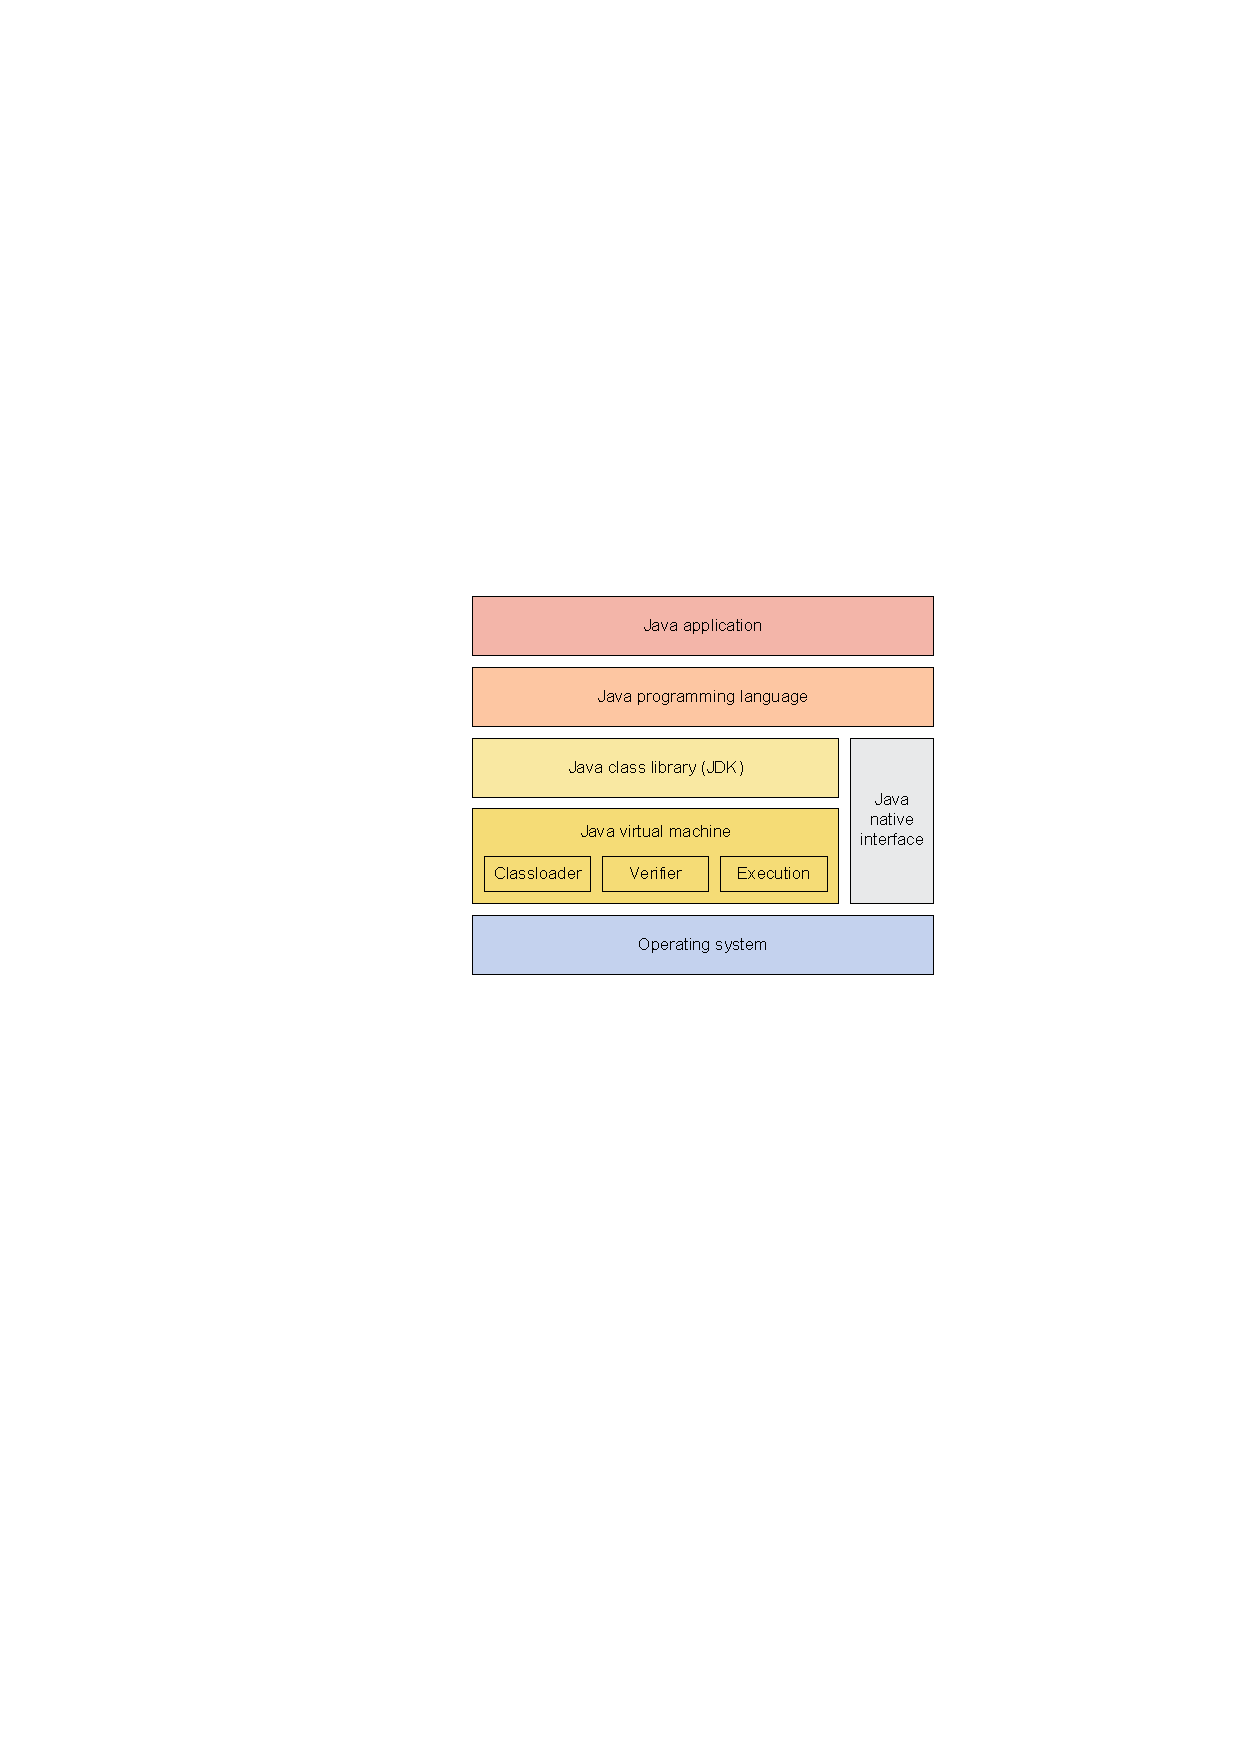
\includegraphics[scale=\picscale]{intro/java_overview}
    \caption{Java system overview}
    \label{fig:java:overview}
\end{figure*}
%
As can be seen in \figurename~\ref{fig:java:overview}, Java consists
of three main components:
%
\begin{enumerate}
    \item The Java programming language as defined in
    \cite{JavaLangSpec2}
    \item The class library, defined as part of the Java
        specification. All implementations of Java have to
        contain the library as defined by Sun
    \item The Java virtual machine (defined in \cite{jvm}) that loads,
     verifies and executes the binary representation (the
\emph{class file}) of a Java program
\end{enumerate}
%
The Java native interface supports functions written in C or C++.
This combination is sometimes called \emph{Java technology} to
emphasize the fact that Java is more than just another
object-oriented language.

However, a number of issues have hindered a broad acceptance of
Java. The original presentation of Java as an Internet language led
to the misconception that Java was not a general-purpose programming
language. Another obstacle was the first implementation of the JVM
as an interpreter. Execution of Java programs was \emph{very} slow
compared to compiled C/C++ programs. Although advances in its
runtime technology, in particular the just-in-time compiler, have
closed the performance gap, it is still a commonly held view that
Java is slow.

\subsection{History}

The Java programming language originated as part of a research
project to develop software for network devices and embedded
systems. In the early '90s, Java, which was originally known as Oak
\cite{java:oak, java:oak2}, was created as a programming tool for a
consumer device that we would today call a PDA. The device (known as
*7) was a small SPARC-based hardware device with a tiny embedded OS.
However, the *7 was not issued as a product and Java was officially
released in 1995 as a new language for the Internet (to be
integrated into Netscape's browser). Over the years, Java technology
has become a programming tool for desktop applications, web servers
and server applications. These application domains resulted in the
split of the Java platform into the Java standard edition (J2SE) and
the enterprise edition (J2EE) in 1999. With every new release, the
library (defined as part of the language) continued to grow. Java
for embedded systems was clearly not an area Sun was interested in
pursuing. However, with the arrival of mobile phones, Sun again
became interested in this embedded market. Sun defined different
subsets of Java, which have now been combined into the Java Micro
Edition (J2ME). A detailed description of the J2ME follows in
Section~\ref{sec:j2me}.


\subsection{The Java Programming Language}

The Java programming language is a general-purpose object-oriented
language. Java is related to C and C++, but with a number of aspects
omitted. Java is a strongly typed language, which means that type
errors can be detected at compile time. Other errors, such as wrong
indices in an array, are checked at runtime. The
problematic\footnote{C pointers represent memory addresses as data.
Pointer arithmetic and direct access to memory leads to common and
hard-to-find program errors.} \emph{pointer} in C and explicit
deallocation of memory is completely avoided. The pointer is
replaced by a \emph{reference}, i.e.\ an abstract pointer to an
object. Storage for an object is allocated from the heap during
creation of the object with \code{new}. Memory is freed by automatic
storage management, typically using a garbage collector. The garbage
collector avoids memory leaks from a missing \code{free()} and the
safety problems exposed by dangling pointers.

The types in Java are divided into two categories: primitive types
and reference types. \tablename~\ref{tab:java:primitive} lists the
available primitive types. Method local variables, class fields and
object fields contain either a primitive type value or a reference
to an object.

\begin{table}
    \centering
    \begin{tabular}{ll}
        \toprule
        Type & Description \\
        \midrule
        \code{boolean} & either \code{true} or \code{false} \\
        \code{char} & 16-bit Unicode character (unsigned) \\
        \code{byte} & 8-bit integer (signed) \\
        \code{short} & 16-bit integer (signed) \\
        \code{int} & 32-bit integer (signed) \\
        \code{long} & 64-bit integer (signed) \\
        \code{float} & 32-bit floating-point (IEEE 754-1985) \\
        \code{double} & 64-bit floating-point (IEEE 754-1985) \\
        \bottomrule
    \end{tabular}
    \caption{Java primitive data types}
    \label{tab:java:primitive}
\end{table}

Classes and class instances, the objects, are the fundamental data
and code organization structures in Java. There are no global
variables or functions as there are in C/C++. Each method belongs to
a class. This `everything belongs to a class or an object' combined
with the class naming convention, as suggested by Sun, avoids name
conflicts in even the largest applications.

New classes can extend exactly one superclass. Classes that do not
explicitly extend a superclass become direct subclasses of
\code{Object}, the root of the whole class tree. This single
inheritance model is extended by \emph{interfaces}. Interfaces are
abstract classes that only define method signatures and provide no
implementation. A concrete class can implement several interfaces.
This model provides a simplified form of multiple inheritance.

Java supports multitasking through \emph{threads}. Each thread is a
separate flow of control, executing concurrently with all other
threads. A thread contains the method stack as thread local data --
all objects are shared between threads. Access conflicts to shared
data are avoided by the proper use of \code{synchronized} methods or
code blocks.

Java programs are compiled to a machine-independent bytecode
representation as defined in \cite{jvm}. Although this intermediate
representation is defined for Java, other programming languages
(e.g.\ ADA \cite{269646}) can also be compiled into Java bytecodes.

\section{The Java Virtual Machine}

The Java virtual machine (JVM) is a definition of an abstract
computing machine that executes bytecode programs. The JVM
specification \cite{jvm} defines three elements:
\begin{itemize}
    \item An instruction set and the meaning of those instructions
    -- the \emph{bytecodes}
    \item A binary format -- the \emph{class file} format. A
    class file contains the bytecodes, a symbol table and other
    ancillary information
    \item An algorithm to \emph{verify} that a class file
    contains valid programs
\end{itemize}
%
In the solution presented in this book, the class files are
verified, linked and transformed into an internal representation
before being executed on JOP. This transformation is performed with
\cmd{JOPizer} and is not executed on JOP. We will therefore omit the
description of the class file and the verification process.

The instruction set of the JVM is stack-based. All operations take
their arguments from the stack and put the result onto the stack.
Values are transferred between the stack and various memory areas.
We will discuss these memory areas first, followed by an explanation
of the instruction set.

\subsection{Memory Areas}

The JVM contains various runtime data areas. Some of these areas are
shared between threads, whereas other data areas exist separately
for each thread.

\begin{description}
    \item[Method area:]
The method area is shared among all threads. It contains static
class information such as field and method data, the code for the
methods and the constant pool. The constant pool is a per-class
table, containing various kinds of constants such as numeric values
or method and field references. The constant pool is similar to a
symbol table.

Part of this area, the code for the methods, is very frequently
accessed (during instruction fetch) and therefore is a good
candidate for caching.

    \item[Heap:]
The heap is the data area where all objects and arrays are
allocated. The heap is shared among all threads. A garbage collector
reclaims storage for objects.

    \item[JVM stack:]
Each thread has a private stack area that is created at the same
time as the thread. The JVM stack is a logical stack that contains
following elements:
\begin{enumerate}
    \item A frame that contains return information for a method
    \item A local variable area to hold local values inside a method
    \item The operand stack, where all operations are performed
\end{enumerate}
%
Although it is not strictly necessary to allocate all three elements
to the same type of memory we will see in Section~\ref{sec:stack}
that the argument-passing mechanism regulates the layout of the JVM
stack.

Local variables and the operand stack are accessed as frequently
as registers in a standard processor. A Java processor should
provide some caching mechanism of this data area.

\end{description}
%
The memory areas are similar to the various segments in conventional
processes (e.g.\ the method code is analogous to the `text'
segment). However, the operand stack replaces the registers in a
conventional processor.

\subsection{JVM Instruction Set}

The instruction set of the JVM contains 201 different instructions
\cite{jvm}. This \emph{bytecodes} can be grouped into the following
categories:
%
\begin{description}
    \item[Load and store:]
Load instructions push values from the local variables onto the
operand stack. Store instructions transfer values from the stack
back to local variables. 70 different instructions belong to this
category. Short versions (single byte) exist to access the first
four local variables. There are unique instructions for each basic
type (\code{int}, \code{long}, \code{float}, \code{double} and
\code{reference}). This differentiation is necessary for the
bytecode verifier, but is not needed during execution. For example
\code{iload}, \code{fload} and \code{aload} all transfer one 32-bit
word from a local variable to the operand stack.

    \item[Arithmetic:]
The arithmetic instructions operate on the values found on the stack
and push the result back onto the operand stack. There are
arithmetic instructions for \code{int}, \code{float} and
\code{double}. There is no direct support for \code{byte},
\code{short} or \code{char} types. These values are handled by
\code{int} operations and have to be converted back before being
stored in a local variable or an object field.

    \item[Type conversion:]
The type conversion instructions perform numerical conversions
between all Java types: as implicit widening conversions (e.g.\
\code{int} to \code{long}, \code{float} or \code{double}) or
explicit (by casting to a type) narrowing conversions.

    \item[Object creation and manipulation:]
Class instances and arrays (that are also objects) are created and
manipulated with different instructions. Objects and class fields
are accessed with type-less instructions.

    \item[Operand stack manipulation:]
All direct stack manipulation instructions are type-less and
operate on 32-bit or 64-bit entities on the stack. Examples of these
instructions are \code{dup}, to duplicate the top operand stack
value, and \code{pop}, to remove the top operand stack value.

    \item[Control transfer:]
Conditional and unconditional branches cause the JVM to continue
execution with an instruction other than the one immediately
following. Branch target addresses are specified relative to the
current address with a signed 16-bit offset. The JVM provides a
complete set of branch conditions for \code{int} values and
references. Floating-point values and type \code{long} are
supported through compare instructions. These compare instructions
result in an \code{int} value on the operand stack.

    \item[Method invocation and return:]
The different types of methods are supported by four instructions:
invoke a class method, invoke an instance method, invoke a method
that implements an interface and an \code{invokespecial} for an
instance method that requires special handling, such as
\code{private} methods or a superclass method.


\end{description}
%
A bytecode consists of one instruction byte followed by optional
operand bytes. The length of the operand is one or two bytes, with
the following exceptions: \code{multianewarray} contains 3 operand
bytes; \code{invokeinterface} contains 4 operand bytes, where one is
redundant and one is always zero; \code{lookupswitch} and
\code{tableswitch} (used to implement the Java \code{switch}
statement) are variable-length instructions; and \code{goto\_w} and
\code{jsr\_w} are followed by a 4 byte branch offset, but neither is
used in practice as other factors limit the method size to 65535
bytes.

\subsection{Methods}

A Java \emph{method} is equivalent to a \emph{function} or
\emph{procedure} in other languages. In object oriented terminology
this \emph{method} is \emph{invoked} instead of \emph{called}. We
will use \emph{method} and \emph{invoke} in the remainder of this
text. In Java and the JVM, there are five types of methods:
%
\begin{itemize}
    \item Static or class methods
    \item Virtual methods
    \item Interface methods
    \item Class initialization
    \item Constructor of the parent class (\code{super()})
\end{itemize}
%
For these five types there are only four different bytecodes:
\begin{description}
    \item[\code{invokestatic}:] A class method (declared \code{static})
    is invoked. As the target does not depend on an object, the
    method reference can be resolved at load/link time.

    \item[\code{invokevirtual}:] An object reference is resolved and
    the corresponding method is invoked. The resolution is usually
    done with a dispatch table per class containing all implemented and
    inherited methods. With this dispatch table, the resolution can
    be performed in constant time.

    \item[\code{invokeinterface}:] An interface allows Java
    to emulate multiple inheritance. A class can implement several
    interfaces, and different classes (that have no inheritance
    relation) can implement the same interface. This flexibility
    results in a more complex resolution process. One method of
    resolution is a search through the class hierarchy that results
    in a variable, and possibly lengthy, execution time. A constant time
    resolution is possible by assigning every interface method a
    unique number. Each class that implements an interface needs its
    own table with unique positions for each interface method of
    the \emph{whole} application.

    \item[\code{invokespecial}:] Invokes an instance method with
    special handling for superclass, \code{private}, and instance
    initialization. This bytecode catches many different cases.
    This results in expensive checks for common \code{private} instance
    methods.
\end{description}
%

\subsection{Implementation of the JVM}

There are several different ways to implement a virtual machine. The
following list presents these possibilities and analyses how
appropriate they are for embedded devices.
%
\begin{description}
    \item[Interpreter:]
The simplest realization of the JVM is a program that interprets the
bytecode instructions. The interpreter itself is usually written in
C and is therefore easy to port to a new computer system. The
interpreter is very compact, making this solution a primary choice
for resource-constrained systems. The main disadvantage is the high
execution overhead. From a code fragment of the typical interpreter
loop, as shown in Listing~\ref{lst:intro:java:intprt}, we can
examine the overhead: The emulation of the stack in a high-level
language results in three memory accesses for a simple \code{iadd}
bytecode. The instruction is decoded through an indirect jump.
Indirect jumps are still a burden for standard branch prediction
logic.

\begin{lstlisting}[float,caption={Typical JVM interpreter loop},
label=lst:intro:java:intprt]
    for (;;) {
        instr = bcode[pc++];
        switch (instr) {
            ...
            case IADD:
                tos = stack[sp]+stack[sp-1];
                --sp;
                stack[sp] = tos;
                break;
            ...
        }
    }
\end{lstlisting}

    \item[Just-In-Time Compilation:]
Interpreting JVMs can be enhanced with just-in-time (JIT) compilers.
A JIT compiler translates Java bytecodes to native instructions
during runtime. The time spent on compilation is part of the
application execution time. JIT compilers are therefore restricted
in their optimization capacity. To reduce the compilation overhead,
current JVMs operate in mixed mode: Java methods are executed in
interpreter mode and the call frequency is monitored. Often-called
methods, the hot spots, are then compiled to native code.

JIT compilation has several disadvantages for embedded systems,
notably that a compiler (with the intrinsic memory overhead) is
necessary on the target system. Due to compilation during
runtime, execution times are hardly predictable.\footnote{Even if
the time for the compilation is known, the WCET for a method has
to include the compile time! Furthermore, WCET analysis has to
know in advance what code will be produced by JIT compilation.}

    \item[Batch Compilation:]
Java can be compiled, in advance, to the native instruction set of
the target. Precompiled libraries are linked with the application
during runtime. This is quite similar to C/C++ applications with
shared libraries. This solution undermines the flexibility of Java:
dynamic class loading during runtime. However, this is not a major
concern for embedded systems.


    \item[Hardware Implementation:]
A Java processor is the implementation of the JVM in hardware. The
JVM bytecode is the native instruction set of such a processor. This
solution can result in quite a small processor, as a stack
architecture can be implemented very efficiently. A Java processor
is memory-efficient as an interpreting JVM, but avoids the execution
overhead. The main disadvantage of a Java processor is the lack of
capability to execute C/C++ programs.

\end{description}

\subsection{Embedded Java}

\begin{figure}
    \centering
    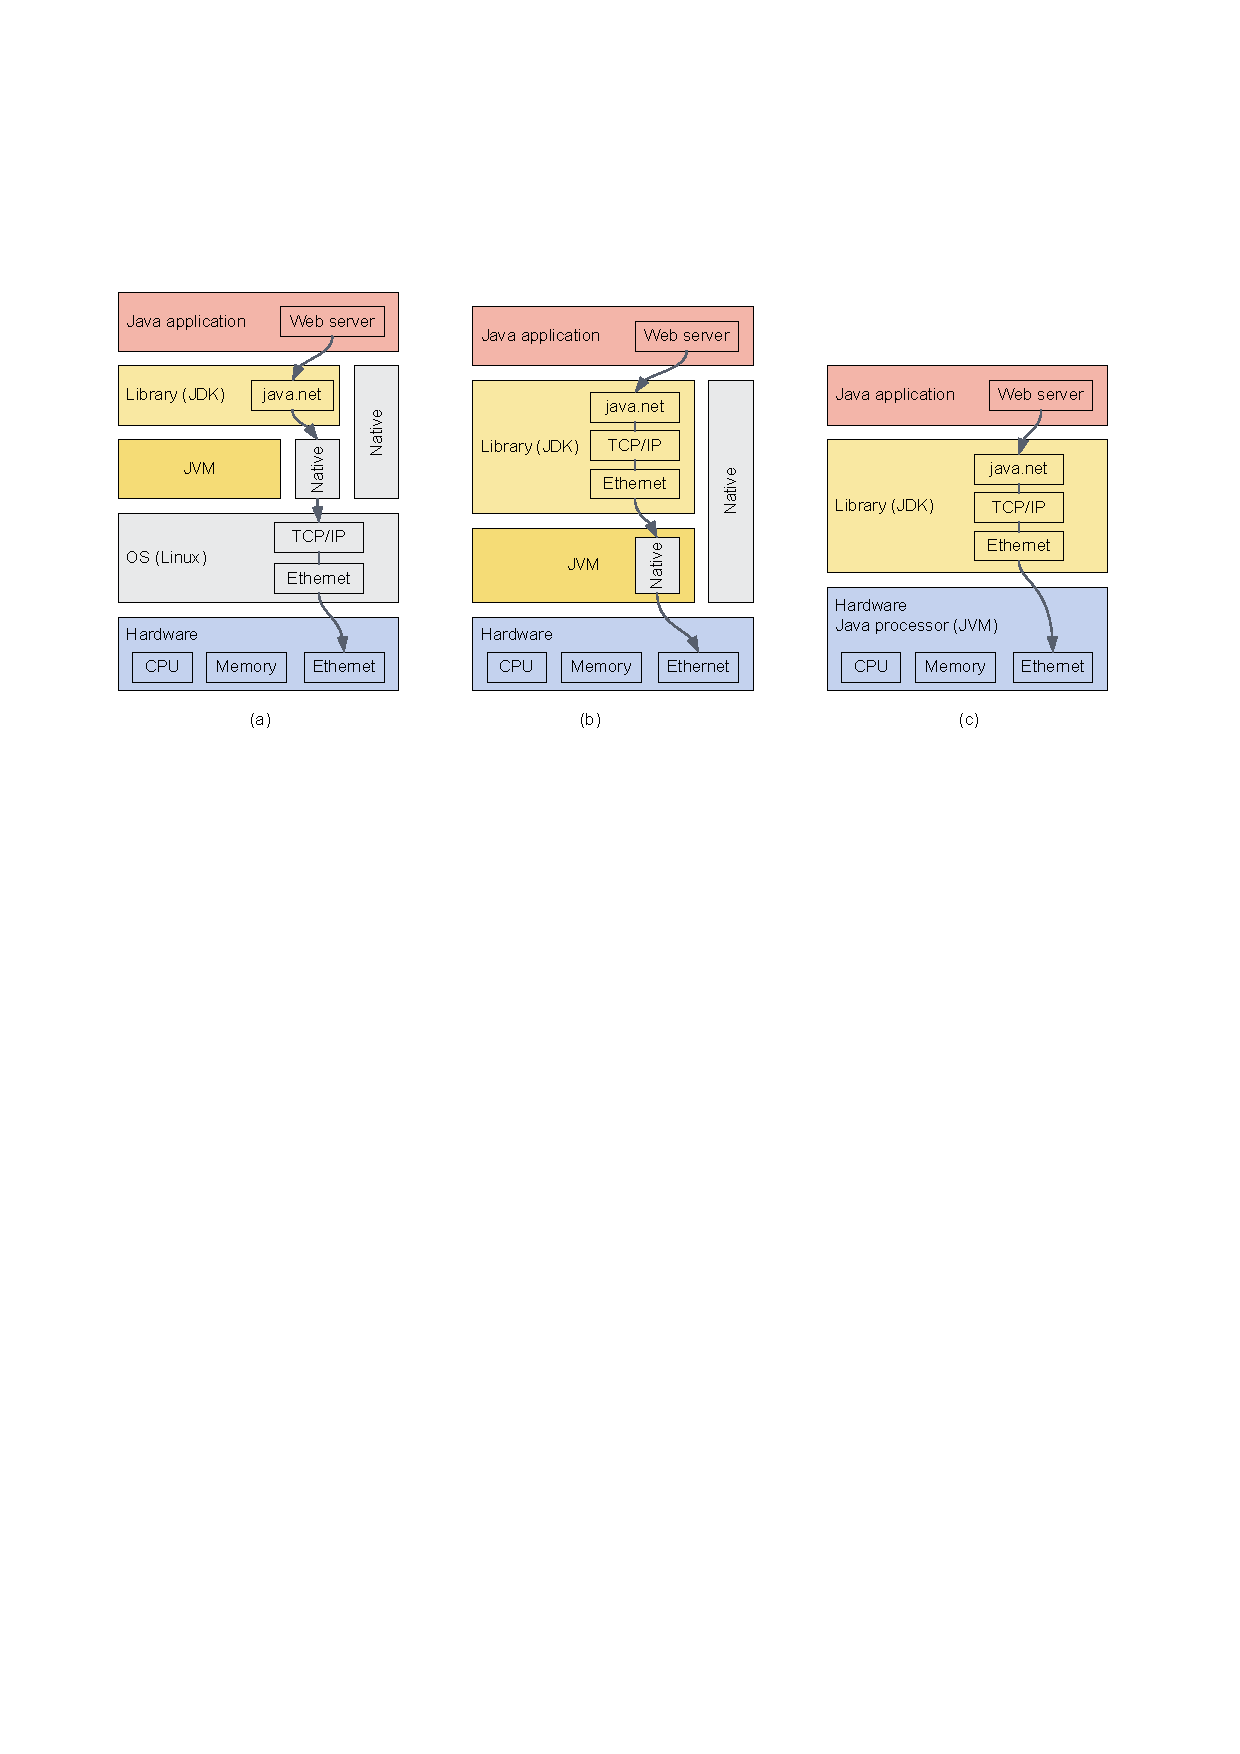
\includegraphics[width=\textwidth]{intro/jvmall}
    \caption{Implementation variations for an embedded JVM: (a) standard layers
    for Java with an operating system -- equivalent to desktop configurations, (b) a JVM on the bare metal,
    and (c) a JVM as a Java processor.}\label{fig:java:embedded}
\end{figure}

In embedded systems the architecture of JVMs are more diverse than
on desktop or server systems. Figure~\ref{fig:java:embedded} shows
variations of Java implementations in embedded systems and an
example of the control flow for a web server application. The
standard approach of a JVM running on top of an operating system
(OS) is shown in sub-figure (a). A network connection bypasses the
JVM via native functions and uses the TCP/IP stack implementation
and the device drivers of the OS.

A JVM without and OS is shown in sub-figure (b). This solution is
often called \emph{running on the bare metal}. The JVM acts as the OS
and provides the thread scheduling and the low-level access to the
hardware. In that case the network stack can be written entirely in
Java. JNode\footnote{\url{http://www.jnode.org/}} is an approach to
implement the OS entirely in Java. This solution becomes popular even
in server applications.\footnote{BEA System offers the JVM LiquidVM
that includes basic OS functions and does not need a guest OS.
%\url{http://www.bea.com/framework.jsp?CNT=index.htm&FP=/content/products/weblogic/virtual_server}
}

Sub-figure (c) shows an embedded solution where the JVM is part of
the hardware layer. That means it is implemented in a Java
processor. With this solution the native layer can be completely
avoided and all code (application and system code) is written
entirely in Java.

Figure~\ref{fig:java:embedded} shows how the flow from the
application goes down to the hardware. The example consists of a web
server and an Internet connection via Ethernet. In case (a) the
application web server talks with \code{java.net} in the JDK. The
flow goes through a native interface to the TCP/IP implementation and
the Ethernet device driver within the OS (usually written in C). The
device driver talks with the Ethernet chip. In (b) the OS layer is
omitted: the TCP/IP layer and the Ethernet device driver are now part
of the Java library. In (c) the JVM is part of the hardware layer and
a direct access from the Ethernet driver to the Ethernet hardware is
mandatory. Note how part of the network stack moves up from the OS
layer to the Java library. Version (c) shows a pure Java
implementation of the whole network stack.


\section{Summary}

Java is a unique combination of the language definition, a rich
class library and a runtime environment. A Java program is compiled
to bytecodes that are executed by a Java virtual machine. Strong
typing, runtime checks and avoidance of pointers make Java a
\emph{safe} language. The intermediate bytecode representation
simplifies porting of Java to different computer systems. An
interpreting JVM is easy to implement and needs few system
resources. However, the execution speed suffers from interpreting.
JVMs with a just-in-time compiler are state-of-the-art for desktop
and server systems. These compilers require large amounts of memory
and have to be ported for each processor architecture, which means
they are not the best choice for embedded systems. A Java processor
is the implementation of the JVM as a concrete machine. A Java
processor avoids the slow execution model of an interpreting JVM and
the memory requirements of a compiler, thus making it an interesting
execution system for Java in embedded systems.


%% This chapter is removed as it is found in the thesis.
%% We can probably recycle some text for the embedded seciton in
%% former chapter.
%%
%\chapter{Java for Embedded Real-Time Systems}
%%\emph{Shall we keep this one? Or better SCJ/RtThread description
%%(with some of general Java ME related stuff -- shorter.}
%
%\label{chap:rtjava}
%    Java was created as a part of the Green project specifically for an
embedded device, a handheld wireless PDA. The device was never
released as a product and Java was launched as the \emph{new}
language for the Internet. Over time, Java become very popular to
build desktop applications and web services. However, embedded
systems are still programmed in C or C++. The pragmatic approach of
Java to object orientation, the huge standard library and
enhancements over C lead to a productivity increase, which now also
attracts embedded system programmers. A built-in concurrency model
and an elegant language construct to express synchronization between
threads also simplify typical programming idioms in this area.

On the other hand, there are some issues with Java in an embedded
system. Embedded systems are usually too small for JIT-compilation
resulting in a slow interpreting execution model. Moreover, a major
problem for embedded systems, which are usually also real-time
systems, is the under specification of the scheduler. Even an
implementation without preemption is allowed. The intention for this
\textit{loose} definition of the scheduler is to be able to
implement the JVM on many platforms where no good multitasking
support is available. The Real Time Specification for Java (RTSJ)
\cite{rtsj}  addresses many of these problems.

This section summarizes the issues with standard Java on embedded
systems and describes various definitions for small devices given by
Sun. It is followed by an overview of the two real-time extensions of
Java and approaches for restricting the RTSJ for high-integrity
applications. If, and how, these specifications are sufficient for
small embedded systems in general, and specifically for JOP, is
analyzed. The missing definition for small embedded real-time systems
is provided in Section~\ref{sec:rtprof}.

\section{Java Support for Embedded Systems}

When not using the cyclic executive approach, programming of
embedded (real-time) systems is all about concurrent programming
with time constraints. The basic functions can be summarized as:

\begin{itemize}
    \item Threads
    \item Communication
    \item Activation
    \item Low level hardware access
\end{itemize}

\paragraph{Threads and Communication}

Java has a built-in model for concurrency, the class \code{Thread}.
All threads share the same heap resulting in a shared memory
communication model. Mutual exclusion can be defined on methods or
code blocks with the keyword \code{synchronized}. Synchronized
methods acquire a lock on the object of the method. For synchronized
code blocks, the object to be locked is explicitly stated.


\paragraph{Activation}

Every object inherits the methods \code{wait()}, \code{notify()} and
\code{notifyAll()} from \code{Object}. These methods in conjunction
with synchronization on the object support activation. The classes
\code{java.util.TimerTask} and \code{java.util.Timer} (since JDK
1.3) can be used to schedule tasks for future execution in a
background thread.

\section{Issues with Java in Embedded Systems}

Although Java has language features that simplify concurrent
programming, the definition of these features is too vague for
real-time systems.


\paragraph{Threads and Synchronization}

Java, as described in \cite{JavaLangSpec2}, defines a very loose
behavior of threads and scheduling. For example, the specification
allows even low priority threads to preempt high priority threads.
This protects threads from starvation in general purpose
applications, but is not acceptable in real-time programming. Wakeup
of a single thread with \code{notify()} is not precisely defined:
\textit{the choice is arbitrary and occurs at the discretion of the
implementation.} It is not mandatory for a JVM to deal with the
priority inversion problem. No notation of periodic activities,
which are common in embedded systems programming, is available with
the standard \code{Thread} class.

\paragraph{Garbage Collector}

Garbage collection greatly simplifies programming and helps to avoid
classic programming errors (e.g.\ memory leaks). Although real-time
garbage collectors evolve, they are usually avoided in hard
real-time systems. A more conservative approach to memory allocation
is necessary.

\paragraph{WCET on Interfaces (OOP)}

Method overriding and Interfaces, the simplified concept of multiple
inheritance in Java, are the key concepts in Java to support object
oriented programming. Like function pointers in C, the dynamic
selection of the actual function at runtime complicates WCET
analysis. Implementation of interface look up usually requires a
search of the class hierarchy at runtime or very large dispatch
tables.

\paragraph{Dynamic Class Loading}

Dynamic class loading requires the resolution and verification of
classes. This is a function that is usually too complex (and
consumes too much memory) for embedded devices. An upper bound of
execution time for this function is almost impossible to predict (or
too large). This results in the complete avoidance of dynamic class
loading in real-time systems.

\paragraph{Standard Library}

For an implementation to be Java-conformant, it must include the
full library (JDK). The JAR files for this library constitute about
15~MB (in JDK 1.3, without native libraries), which is far too large
for many embedded systems. Since Java was designed to be a safe
language with a safe execution environment, no classes are defined
for low-level access of hardware features. The standard library was
not defined and coded with real-time applications in mind.

\paragraph{Execution Model}

The first execution model for the JVM was an interpreter. The
interpreter is now enhanced with Just-In-Time (JIT) compilation.
Interpreting Java bytecodes is too slow and JIT compilation is not
applicable in real-time systems. The time for the compilation
process had to be included in the WCET, resulting in impracticable
values.

\paragraph{Class Initialization Issues}
\label{para:restrict:clinit}

According to \cite{jvm} the static initializers of a class C are
executed immediately before one of the following occurs: (i) an
instance of C is created; (ii) a static method of C is invoked or
(iii) a static field of C is used or assigned. The issue with this
definition is that it is not allowed to invoke the static
initializers at JVM startup and it is not so obvious when it gets
invoked.

It follows that the bytecodes \code{getstatic}, \code{putstatic},
\code{invokestatic} and \code{new} can lead to class initialization
and the possibility of high WCET values. In the JVM, it is necessary
to check every execution of these bytecodes if the class is already
initialized. This leads to a loss of performance and is violated in
some existing implementations of the JVM. For example, the first
version of CACAO \cite{cacao} invokes the static initializer of a
class at compilation time. Listing~\ref{lst:retrict:clinit} shows an
example of this problem.

\cmd{JOPizer} tries to find a correct order of the class
initializers and puts this list into the application file. If a
circular dependency is detected the application will not be built.
The class initializers are invoked at JVM startup.

\begin{lstlisting}[float,caption={Class initialization can occur very late},
label=lst:retrict:clinit]
    public class Problem {

        private static Abc a;
        public static int cnt; // implicitly set to 0

        static {
            // do some class initializaion
            a = new Abc();  //even this is ok.
        }

        public Problem() {
            ++cnt;
        }
    }

    // anywhere in some other class, in situation,
    // when no instance of Problem has been created
    // the following code can lead to
    // the execution of the initializer
    int nrOfProblems = Problem.cnt;

\end{lstlisting}

\paragraph{Synchronization Issue}

Synchronization is possible with methods and on code blocks. Each
object has a monitor associated with it and there are two different
ways to gain and release ownership of a monitor. Bytecodes
\code{monitorenter} and \code{monitorexit} explicitly handle
synchronization. In other cases, synchronized methods are marked in
the class file with the access flags. This means that all bytecodes
for method invocation and return must check this access flag. This
results in an unnecessary overhead on methods without
synchronization. It would be preferable to encapsulate the bytecode
of synchronized methods with bytecodes \code{monitorenter} and
\code{monitorexit}. This solution is used in Suns picoJava-II
\cite{pjProgRef}. The code is manipulated in the class loader. Two
different ways of coding synchronization, in the bytecode stream and
as access flags, are inconsistent.

\section{Java Micro Edition}
\label{sec:j2me}

The definition of Java also includes the definition of the class
library (JDK). This is a huge library\footnote{In JDK 1.4 the main
runtime library, rt.jar, is 25~MB.} and too large for some systems.
To compensate for this Sun has defined the \textit{Java 2 Platform,
Micro Edition} (J2ME) \cite{J2ME}. As Sun has changed the focus of
Java targets several times, the specifications reflect this through
their slightly chaotic manner. J2ME reduces the function of the JVM
(e.g. no floating point support) to make implementation easier on
smaller processors. It also reduces the library (API). J2ME defines
three layers of software built upon the host operating system of the
device:
%
\begin{description}
    \item[Java Virtual Machine:] This layer is just the JVM as in every Java
implementation. Sun has assumed that the JVM will be implemented on
top of a host operating system. There are no additional definitions
for the J2ME in this layer.

    \item[Configuration:] The configuration defines the minimum set of JVM features
and Java class libraries available on a particular category of
devices. In a way, a configuration defines the lowest common
denominator of the Java platform features and libraries that the
developers can assume to be available on all devices.

    \item[Profile:] The profile defines the minimum set of Application
Programming Interfaces (APIs) available on a particular family of
devices. Profiles are implemented upon a particular configuration.
Applications are written for a particular profile and are thus
portable to any device that supports that profile. A device can
support multiple profiles.

\end{description}
%
There is an overlap of the layers \textit{configuration} and
\textit{profile}: Both define/restrict Java class libraries. Sun
states: `\textit{A profile is an additional way of specifying the
subset of Java APIs, class libraries, and virtual machine features
that targets a specific family of devices.'} However, in the current
available definitions JVM features are only specified in
\textit{configurations}.

\subsection{Connected Limited Device Configuration (CLDC)}
\label{subsec:cldc}

CLDC is a configuration for connected devices with at least 192~KB
of total memory and a 16-bit or 32-bit processor. As the main target
devices are cellular phones, this configuration has become very
popular (Sun: `\textit{CLDC was designed to meet the rigorous memory
footprint requirements of cellular phones.}'). The CLDC is composed
of the K Virtual Machine (KVM) and core class libraries. The
following features have been removed from the Java language
definition:
%
\begin{itemize}
    \item Floating point support
    \item Finalization
\end{itemize}
%
Error handling has been altered so that the JVM halts in an
implementation-specific manner. The following features have been
removed from the JVM:
%
\begin{itemize}
    \item Floating point support
    \item Java Native Interface (JNI)
    \item Reflection
    \item Finalization
    \item Weak references
    \item User-defined class loaders
    \item Thread groups and daemon threads
    \item Asynchronous exceptions
    \item Data type \code{long} is optional
    \item \code{wait()}, \code{notify()}, and \code{notifyAll()}
\end{itemize}
%
These restrictions are defined in the final version 1.0 of CLDC. A
newer version (1.1) again adds floating-point support.

The CLDC defines a subset of the following Java class libraries:
\code{java.io}, \code{java.lang}, \code{java.lang.ref} and
\code{java.util}. An additional library
(\code{javax.\linebreak[4]microedition.io}) defines a simpler
interface for communication than \code{java.io} and \code{java.net}.
Examples of connections are: HTTP, datagrams, sockets and
communication ports.

A small-footprint JVM, known as the K Virtual Machine (KVM), is part
of the CLDC distribution. KVM is suitable for 16/32-bit
microprocessors with a total memory budget of about 128~KB.

When implementing CLDC, one may choose to preload/prelink some
classes. A utility (\textit{JavaCodeCompact}) combines one or more
Java class files and produces a C file that can be compiled and
linked directly with the KVM.

There is only one profile defined under CLDC: the Mobile Information
Device Profile (MIDP) defines a user interface for LC displays,
a media player and a game API.

\subsection{Connected Device Configuration (CDC)}

The CDC defines a configuration for devices with a network connection
and assumes a minimum of a 32-bit processor and 2~MB memory. CDC
defines no restrictions for the JVM. A virtual machine, the CVM, is
part of the distribution. The CVM expects the following functionality
from the underlying OS:
%
\begin{itemize}
    \item Threads
    \item Synchronization (mutexes and condition variables)
    \item Dynamic linking
    \item malloc (POSIX memory allocation utility) or equivalent
    \item Input/output (I/O) functions
    \item Berkeley Standard Distribution (BSD) sockets
    \item File system support
    \item Function libraries must be thread-safe. A thread blocking in a library should not block any other VM threads.
\end{itemize}
%
The tools \textit{JavaCodeCompact} and \textit{JavaMemberDepend} are
part of the distribution. \textit{JavaMemberDepend} generates lists
of dependencies at the class member level. The existence of
\textit{JavaCodeCompact} implies that preloading of classes is
allowed in CDC. Three profiles are defined for CDC:
%
\begin{description}
    \item[Foundation Profile] is a set of Java APIs that support resource-constrained
devices without a standards-based GUI system. The basic class
libraries from the Java standard edition (\code{java.io},
\code{java.lang} and \code{java.net}) are supported and a connection
framework (\code{javax.microedition.io}) is added.

    \item[Personal Basis Profile] is a set of Java APIs that support
resource-constrained devices with a standards-based GUI framework
based on lightweight components. It adds some parts of the Abstract
Window Toolkit (AWT) support (relative to JDK 1.1 AWT).

    \item[Personal Profile] completes the AWT libraries and includes support for the
applet interface.

\end{description}
%
Although a device can support multiple profiles, additional libraries
for RMI and ODBC are known as \textit{optional packages}.

\subsection{Additional Specifications}

The following specifications do not fit into the layer scheme of
J2ME. However, they are defined in the same way as the above:
subsets of the JVM and subsets/extensions of Java classes (API):
%
\begin{description}
    \item[Java Card] is a definition for the resource-constrained world of smart
cards. The execution lifetime of the JVM is the lifetime of the
card. The JVM is highly restricted (e.g. no threads, data type
\code{int} is optional) and defines a different instructions set
(i.e. new bytecodes to support smaller integer types).

    \item[Java Embedded Server] is an API definition for services such as HTTP.

    \item[Personal Java] was intended as a Java platform on Windows CE
and is now marked as end of life.

    \item[Java TV] is an extension to produce interactive
television content and manage digital media. The description states
that the JVM runs on top of an RTOS, but no real-time specific
extensions are defined.

\end{description}
%
Other than Sun's, the few specifications that exist for embedded
Java are:
%
\begin{description}
    \item[leJOS] \cite{lejos} is a JVM for Lego Mindstorm with stronger restrictions
on the core classes than the CLDC.

    \item[RTDA] \cite{rtda01} although named `Real-Time Data Access' the
definition consists of two parts:

    \begin{itemize}
        \item An I/O data access API specification applicable
        for real-time and non real-time applications.
        \item A minimal set of real-time extensions to enable
        the I/O data access also to cover hard real-time capable
        response handling.
    \end{itemize}
\end{description}

\subsection{Discussion}

Many of the specifications (i.e.\ \textit{configurations} and
\textit{profiles}) are developed using the Java Community Process
(JCP). Although the acronym J2ME implies Java version 2 (i.e. JDK
1.2 and later) almost all technologies under J2ME are still based on
JDK 1.1.

Besides Java Card, CLDC is the `smallest' definition from Sun. It
assumes an operating system and is quite large (the JAR file for the
classes is about 450KB). There are no API definitions for low-level
hardware access. CLDC is not suitable for small embedded devices.
Java Card defines a different JVM instruction set and thus
compromises basic ideas of Java. A more restricted definition with
following features is needed:
%
\begin{itemize}
    \item JVM restrictions, such as in CLDC 1.0
    \item A package for low-level hardware access
    \item A minimum subset of core libraries
    \item Additional profiles for different application domains
\end{itemize}


\section{Real-Time Extensions}

In 1999, a document defining the requirements for real-time Java was
published by NIST \cite{nist99}. Based on these requirements, two
groups defined specifications for real-time Java. A comparison of
these two specifications and a comparison with Ada 95's Real-Time
Annex can be found in \cite{507579}. The following section gives an
overview of these specifications and additional defined restrictions
of the RTSJ.

\subsection{Real-Time Core Extension}

The Real-Time Core Extension \cite{JCons00} is a specification
published under the J Consortium. Two execution environments are
defined: the \textit{Core} environment is the special real-time
component. It can be combined with a traditional JVM, the
\textit{Baseline}. For communication between these two domains,
every Core object has two APIs, one for the Core domain and one for
the Baseline domain. Baseline components can synchronize with Core
components via semaphores.

Two forms of source code are supported to annotate attributes:
\textit{stylized} code with calls of static methods of special
classes and \textit{syntactic} code with new keywords. Syntactic
code has to be processed by a special compiler or preprocessor.

The RT-Core as a specification faded into history. Many of the
proposed concepts can be found in NewMonics (now Aonix) PERC systems
\cite{PERC}. A more detailed description of the RT-Core extensions
can be found in \cite{jop:rtjava}.

\subsection{Real-Time Specification for Java}
\label{sec:rtsj}

The Real-Time Specification for Java (RTSJ) defines a new API with
support from the JVM \cite{rtsj}. The following guiding principles
led to the definition:
%
\begin{itemize}
    \item No restriction of the Java runtime environment
    \item Backward compatibility for non-real-time Java programs
    \item No syntactic extension to the Java
language or new keywords
    \item Predictable execution
    \item Address current real-time system practice
    \item Allow future implementations to add advanced features
\end{itemize}
%
A reference implementation (RI) of the RTSJ forms part of the
specification. The RTSJ is backward compatible with existing
non-real-time Java programs, which implies that the RTSJ is intended
to run on top of J2SE (and not on J2ME). The following section
presents an overview of the RTSJ.

\paragraph{Threads and Scheduling}

The behavior of the scheduler is more clearly defined than in
standard Java. A priority-based, preemptive scheduler with at least
28 real-time priorities is defined as the base scheduler. Additional
levels (ten) for the traditional Java threads need to be available.
Threads with the same priority are queued in FIFO order. Additional
schedulers (e.g. EDF) can be provided by the RTSJ implementation. The
class \code{Scheduler} and associated classes provide optional
support for feasibility analysis.


Any instances of classes that implement the interface
\code{Schedulable} are scheduled. In the RTSJ \code{RealtimeThread},
\code{NoHeapRealtimeThread}, and \code{AsyncEventHandler} are
\textit{schedulable objects}. \code{NoHeapRealtimeThread} has and
\code{AsyncEventHandler} can have a priority higher than the garbage
collector. As the available release-parameters indicate, threads are
either periodic or bound to asynchronous events. Threads can be
grouped together to bind the execution cost and deadline for a
period.

\paragraph{Memory}

As garbage collection is problematic in real-time applications, the
RTSJ defines new memory areas:
%
\begin{description}
    \item[Scoped memory] is a memory area with bounded lifetime. When a scope is
entered (with a new thread or through \code{enter()}), all new
objects are allocated in this memory area. Scoped memory areas can
be nested and shared among threads. On exit of the last thread from
a scope, all finalizers of the allocated objects are invoked and the
memory area is freed.
    \item[Physical memory] is used to control allocation in memories with
different access time.
    \item[Raw memory] allows byte-level access to physical memory or memory-mapped I/O.
    \item[Immortal memory] is a memory area shared between
all threads without a garbage collector. All objects created in this
memory area have the same lifetime as the application (a new
definition of \textit{immortal}).
    \item[Heap memory] is the traditional garbage collected memory area.
\end{description}
%
Maximum memory usage and the maximum allocation rate per thread can
be limited. Strict assignment rules between the different memory
areas have to be checked at runtime by the implementation.

\paragraph{Synchronization}

The implementation of \code{synchronized} has to include an
algorithm to prevent priority inversion. The priority inheritance
protocol is the default and the priority ceiling emulation protocol
can be used on request. Threads waiting to enter a synchronized
block are priority ordered and FIFO ordered within each priority.
Wait free queues are provided for communication between instances of
\code{java.lang.Thread} and \code{RealtimeThread}.

\paragraph{Time and Timers}

Classes to represent relative and absolute time with nanosecond
accuracy are defined. All time parameters are split to a \code{long}
for milliseconds and an \code{int} for nanoseconds within those
milliseconds. Each time object has an associated \code{Clock}
object. Multiple clocks can represent different sources of time and
resolution. This allows for the reduction of queue management
overheads for tasks with different tolerance for jitter. A new type,
rationale time, can be used to describe periods with a requested
resolution over a longer period (i.e. allowing release jitter
between the points of the \textit{outer} period)\footnote{Rationale
time is depreciated in the current version of the specification}.
Timer classes can generate time-triggered events (one shot and
periodic).

\paragraph{Asynchrony}

Program logic representing external world events is scheduled and
dispatched by the scheduler. An \code{AsyncEvent} object represents
an external event (such as a POSIX signal or a hardware interrupt)
or an internal event (through call of \code{fire()}). Event handlers
are associated to these events and can be bound to a regular
real-time thread or represent something \textit{similar} to a
thread. The relationship between events and handlers can be
many-to-many. Release of handlers can be restricted to a minimum
interarrival time.


Java's exception handling is extended to represent asynchronous
transfer of control (ATC). \code{RealtimeThread} overloads
\code{interrupt()} to generate an
\code{AsynchronousInterruptedException} (AIE). The AIE is deferred
until the execution of a method that is willing to accept an ATC.
The method indicates this by including AIE in its throw clause. The
semantics of \code{catch} is changed so that, even when it catches
an AIE, the AIE is still propagated until the \code{happened()}
method of the AIE is invoked. \code{Timed}, a subclass of AIE,
simplifies the programming of timeouts.

\paragraph{Support for the RTSJ}

Implementations of the RTSJ are still rare and under development:
%
\begin{description}
    \item[RI]
is the freely available reference implementation for a Linux system
\cite{rtsj-ri}.

    \item[jRate]
is an open-source implementation \cite{701668} based on
ahead-of-time compilation with the GNU compiler for Java.

    \item[FLEX]
is a compiler infrastructure for embedded systems developed at MIT
\cite{flex}. Real-time Java is implemented with region-based memory
management and a scheduler framework.

    \item[OVM]
is an open-source framework for Java \cite{ovmir2003}. The emphasis
is on a JVM that is compliant with the RTSJ. RTSJ support is based
on the translation of the complete Java application (including the
library) to C and then compiling it into a native executable.

    \item[aJile] (member of the initial JSR-1 expert group) announced the support the RTSJ with CLDC 1.0 on top of
    the aJ-80 and aJ-100 chips. However, the RTSJ was never
    implemented by aJile.

    \item[JamaicaVM] is a RTSJ implementation with a real-time GC by
    aicas.

    \item[IBM] provides a RTSJ implementation combined with the
    Metronome GC \cite{gc:bacon03}.

    \item[Sun's] latest implementation of the RTSJ contains a
    real-time GC developed at Lund University.
\end{description}


\subsection{Discussion of the RTSJ}

The RTSJ is a complex specification leading to a big memory
footprint. The following list shows the size of the main components
of the first RI on Linux:
%
\begin{itemize}
    \item Classes in javax/realtime: 343 KB
    \item All classes in library foundation.jar: 2 MB
    \item Timesys JVM executable: 2.6 MB
\end{itemize}
%
The RTSJ assumes an RTOS and the RI runs on a heavyweight RT-Linux
system. The RTSJ is too complex for low-end embedded systems. This
complexity also hampers programming of high-integrity applications.
The runtime memory allocation of the RTSJ classes is not documented.

\paragraph{Threads and Scheduling}

If a real-time thread is preempted by a higher priority thread, it
is not defined if the preempted thread is placed in front or back of
the waiting queue. The current version (1.0.2) of the
RTSJ\footnote{\url{http://www.rtsj.org/specjavadoc/book_index.html}}
states:
\begin{quote}
A schedulable object that is preempted by a higher priority
schedulable object is placed in the queue for its active priority,
at a position determined by the implementation.
\end{quote}
It is not specified whether the default scheduler performs, or has
to perform, time slicing between threads of equal priority.

\paragraph{Memory}


It would be ideal if real-time systems were able to allocate all
memory during the initialization phase and forbid dynamic memory
allocation in the mission phase. However, this restricts many of
Java's library functions.


The solution to this problem in the RTSJ is \code{ScopedMemory}, a
memory space with limited lifetime. However, it can only be used as
a parameter for thread creation or with \code{enter(Runnable r)}. In
a system without dynamic thread creation, using scoped memory at
creation time of the thread leads to the same behavior as using
immortal memory.

The syntax with \code{enter()} leads to a cumbersome programming
style: for each code part where limited lifetime memory is needed, a
new class has to be defined and a single instance of this class
allocated at initialization time. Trying to solve this problem
elegantly with anonymous classes, as in
Listing~\ref{lst:restr:wrong:scoped} (example from \cite{558498}, p.
623), leads to an error.

\begin{lstlisting}[float,caption={Scoped memory usage with a memory leak},label=lst:restr:wrong:scoped]
    import javax.realtime.*;
    public class ThreadCode implements Runnable
    {
        private void computation()
        {
            final int min = 1*1024;
            final int max = 1*1024;
            final LTMemory myMem = new LTMemeory(min, max);
            myMem.enter(new Runnable()
            {
                public void run()
                {
                    // access to temporary memory
                {
            } );
        }

        public void run()
        {
            ...
            computation();
            ...
        }
    }
\end{lstlisting}


On every call of \code{computation()}, an object of the anonymous
class (and a \code{LTMemory} object) is allocated in immortal
memory, leading to a memory leak. The correct usage of scoped memory
is shown as a code fragment in
Listing~\ref{lst:restr:correct:scoped}. The class \code{UseMem} only
exists to execute the method \code{run()} in scoped memory. One
instance of this class is created outside of the scoped memory.

\begin{lstlisting}[float,caption={Correct usage of scoped memory in the RTSJ},
label=lst:restr:correct:scoped]
    class UseMem implements Runnable {

        public void run() {
            // inside scoped memory
            Integer[] = new Integer[100];
            ...
        }
    }

    // outside of scoped memory
    // in immortal? at initialization?
    LTMemory mem = new LTMemory(1024, 1024);
    UseMem um = new UseMem();

    // usage
    computation() {
        mem.enter(um);
    }
\end{lstlisting}



A simpler\footnote{This syntax is \emph{not} part of the RTSJ. Is is
a suggested change and part of the real-time profile defined in
Section~\ref{sec:rtprof}.} syntax is shown in
Listing~\ref{lst:restr:simple:scoped}. The main drawback of this
syntax is that the programmer is responsible for its correct usage.

\begin{lstlisting}[float,caption={Simpler syntax for scoped memory}
,label=lst:restr:simple:scoped]
    LTMemory myMem;

    // Create the memory object once
    // in the constructor
    MyThread() {
        myMem = new LTMemeory(min, max);
        ...
    }

    public void run() {
        ...
        myMem.enter();
        {   // A new code block disables access
            // to new objects in outer scope.
            // Access to temporary memory:
            Abc a = new Abc();
            ...
        }
        myMem.exit();
        ...
    }
\end{lstlisting}

New objects and arrays of objects have to be initialized to their
default value after allocation \cite{jvm}. This usually results in
zeroing the memory at the JVM level and leads to variable (but
linear) allocation time. This is the reason for the type
\code{LTMemoryArea} in the RTSJ. As suggested in \cite{701668}, this
initialization could be lumped together with the creation time and
exit time of the scoped memory. This results in constant time for
allocation (and usually faster zeroing of the memory).


With the RTSJ memory areas, it is difficult to move data from one
area to another \cite{Niessner03}. This results in a completely
different programming model from that of standard Java. This can
result in the programmer developing his/her own memory management.

One solution to use scoped memory for communication is proposed in
\cite{conf/isorc/PizloFHV04}. A \emph{wedge} thread has to keep the
scope alive when data is added by the producer. The consumer has to
notify this wedge thread when all data is consumed the exit the scope
for the memory recycle. However, there is no single instant available
where we can \emph{guarantee} that the list is empty. A possible
solution for this problem is described in
\cite{conf/isorc/PizloFHV04} as the \emph{handoff} pattern. The
pattern is similar to double buffering, but with an explicit copy of
the data.


\paragraph{Time and Timers }

High resolution time is split into milliseconds and nanoseconds.
Calculation of time differences (an important operation for a
real-time system) is complex with this representation of the time.
In the RI, it is converted to ns for add/subtract. After all mapping
and converting (\code{AbsoluteTime}, \code{HighResolutionTime},
\code{Clock} and \code{RealTimeClock}) the
\code{System.currentTimeMillis()} time, with a ms resolution, is
used.

Since time triggered release of tasks can be modeled with periodic
threads, the additional concept of timers is superfluous.

\paragraph{Asynchronous Events}

An unbound \code{AsyncEventHandler} is not allowed to \code{enter()}
a scoped memory. However, it is not clear if scoped memory is
allowed as a parameter in the construction of a handler.

An unbound \code{AsyncEventHandler} leads to the implicit start of a
thread on an event. This can (and, in the RI, does -- see
\cite{701668}) lead to substantial overheads. From the application
perspective, bound and unbound event handlers behave in the same
way. This is an implementation hint expressed through different
classes. A consistent way to express the \textit{importance} of
events would be a scheduling parameter for the minimum allowed
latency of the handler.

\paragraph{Asynchronous Transfer of Control (ATC)}

The syntax that is used in the throws clause of a method to state
that ATC will be accepted is misleading. Exceptions in \code{throws}
clauses of a method are usually \emph{generated} in that method and
not \textit{accepted}.

\paragraph{J2SE Library}

It is not specified which classes are safe to be used in
\linebreak[4]\code{RealTimeThread} and \code{NoHeapRealTimeThread}.
Several operating system functions can cause unbound blocking and
their usage should be avoided. The memory allocation in standard JDK
methods is not documented and their use in immortal memory context
can lead to memory leaks.

\paragraph{Missing Features}

There is no concept such as start mission. Changing scheduling
parameters during runtime can lead to inconsistent scheduling
behavior.

There is no provision for low-level blocking such as disabling
interrupts. This is a common technique in device drivers where some
hardware operations have to be atomic without affecting the priority
level of the requesting thread (e.g.\ a low priority thread for a
flash file system shall not get preempted during sector write as
some chips internally start the write after a timeout).

\paragraph{On Small Systems}

Many embedded systems are still built with 8 or 16-bit CPUs. 32-bit
processors are seldom used. Java's default integer type is 32-bit,
still large enough for almost all data types needed in embedded
systems. The design decision in the RTSJ to use (often expensive)
64-bit \code{long} data is questionable.

\subsection{Subsets of the RTSJ}
\label{subsec:restr:rtsj}

The RTSJ is complex to implement and applications developed with the
RTSJ are difficult to analyze (because of some of the sophisticated
features of the RTSJ). Various profiles have been suggested for
high-integrity real-time applications that result in restrictions of
the RTSJ.

\subsubsection{A Profile for High-Integrity Real-Time Java Programs}


In \cite{Pusch01}, a subset of the RTSJ for the high-integrity
application domain with hard real-time constraints is proposed. It
is inspired by the Ravenscar profile for Ada \cite{289525} and
focuses on exact temporal predictability.
%
\begin{description}
\item[Application structure:] The application is divided into two
    different phases: \textit{initialization} and
    \textit{mission}. All non time-critical initialization,
    global object allocations, thread creation and startup are
    performed in the initialization phase. All classes need to be
    loaded and initialized in this phase. The mission phase
    starts after returning from \code{main()}, which is assumed
    to execute with maximum priority. The number of threads is
    fixed and the assigned priorities remain unchanged.

\item[Threads:] Two types of tasks are defined: \textit{Periodic
time-triggered activities} execute an infinite loop with at least
one call of \code{waitForNextPeriod()}. \textit{Sporadic activities}
are modeled with a new class \code{SporadicEvent}. A
\code{SporadicEvent} is bound to a thread and an external event on
creation. Unbound event handlers are not allowed. It is not clear if
the event can also be triggered by software (invocation of
\code{fire()}). A restriction for a minimum interarrival time of
events is not defined. Timers are not supported as time-triggered
activities are well supported by periodic threads. Asynchronous
transfers of control, overrun and miss handles and calls to
\code{sleep()} are not allowed.

\item[Concurrency:] Synchronized methods with priority ceiling emulation protocol
provide mutual exclusion to shared resources. Threads are dispatched
in FIFO order within each priority level. Sporadic events are used
instead of \code{wait()}, \code{notify()} and \code{notifyAll()} for
signaling.

\item[Memory:] Since garbage collection is still not
time-predictable, it is not supported. This implicitly converts the
traditional heap to immortal memory. Scoped memory (\code{LTMemory})
is provided for object allocation during the mission phase.
\code{LTMemory} has to be created during the initialization phase
with initial size equal maximum size.

\item[Implementation:] For each thread and for the operations
of the JVM the WCET must be computable. Code is restricted to bound
loops and bound recursions. Annotations for WCET analysis are
suggested. The JVM needs to check the timing of events and thread
execution. It is not stated how the JVM should react to a timing
error.

\end{description}

\subsubsection{Ravenscar-Java}
\label{subsec:rj}

The Ravenscar-Java (RJ) profile \cite{583825} is a restricted subset
of the RTSJ and is based on the work mentioned above. As the name
implies it resembles Ravenscar Ada \cite{289525} concepts in Java.


To simplify the initialization phase, RJ defines \code{Initializer},
a class that has to be extended by the application class which
contains \code{main()}. The use of time scoped memory is further
restricted. \code{LTMemory} areas are not allowed to be nested nor
shared between threads. Traditional Java threads are disallowed by
changing the class \code{java.lang.Thread}. The same is true for all
schedulable objects from the RTSJ. Two new classes are defined:
\begin{itemize}
    \item \code{PeriodicThread} where \code{run()} gets called periodically,
removing the loop construct with \code{waitForNextPeriod()}.
    \item \code{SporadicEventHandler} binds a single thread with a
single event. The event can be an interrupt or a software event.

\end{itemize}

\subsubsection{Safety Critical Java Technology}

A subset of the RTSJ based on the former ideas is under development
under JSR 302\footnote{\url{http://jcp.org/en/jsr/detail?id=302}}.
The subset is intended for Java in safety critical applications that
have to be certified.

\subsubsection{Criticisms on Subsets of the RTSJ}

If a new real-time profile is defined as a subset of the RTSJ it is
harder for the programmer to find out which functions are available
or not. This form of \textit{compatibility} causes confusion. The
use of different classes for a different specification is clearer
and less error prone.

Ravenscar-Java, as a subset of the RTSJ, claims to be compatible
with the RTSJ, in the sense that programs written according to the
profile are valid RTSJ programs. However, mandatory usages of new
classes such as \code{PeriodicThread} need an emulation layer to run
on an RTSJ system. In this case, it is better to define complete new
classes for a subset and provide the mapping to the RTSJ. This
allows a clearer distinction to be made between the two definitions.

It is not necessary to distinguish between heap and immortal memory.
Without a garbage collector, the heap implicitly equals to immortal
memory.

Objects are allocated in immortal memory in the initialization phase.
In the mission phase, no objects should be allocated in immortal
memory. Scoped memory can be entered and subsequent new objects are
allocated in the scoped memory area. Since there are no circumstances
in which allocation in these two memory areas are mixed, no
\code{newInstance()}as defined in the RTSJ is not necessary in a
Ravenscar-Java style profile.

\subsection{Extensions to the RTSJ}

The Distributed Real-Time Specification for Java \cite{Jensen00}
extends RMI within the RTSJ. In 2000, it was accepted in the Sun
Community Process as JSR-50. This specification is still under
development. According to \cite{WellRTSJRMI}, three levels of
integration between the RTSJ and RMI are defined:
%
\begin{description}
    \item[Level 0:] No changes in RMI and the RTSJ are necessary. The proxy thread
on the server acts as an ordinary Java thread. Real-time threads
cannot assume timely delivery of the RMI request.

    \item[Level 1:] RMI is extended to Real-Time RMI. The server
thread is a real-time thread that inherits scheduling parameters
from the calling client.

    \item[Level 2:] RMI and the RTSJ are extended to form the
concept of \textit{distributed real-time threads}. These threads
have a unique system-wide identifier and can move freely in the
distributed system.

\end{description}

JSR-50 is still not finalized. Only minor increments have been
announced at JTRES~2006 and JTRES~2007.

\section{Summary}

In this section, we described definitions for embedded devices given
by Sun. Most of these definitions are targeted for the mobile phone
market and not for classical embedded systems.

Standard Java is under-specified for real-time systems. Two
competing definitions, the `Real-Time Core Extension' and the `Real
Time Specification for Java', address this problem. The RTSJ has
been further restricted for high-integrity applications. A similar
definition that avoids inheritance of complex RTSJ classes is
provided in Section~\ref{sec:rtprof}.


\chapter{JOP Hardware Architecture}
\label{chap:arch}

    \section{Overview of JOP}

This section gives an overview of JOP architecture.
\figurename~\ref{fig:arch:jop:block} shows JOP's major function
units. A typical configuration of JOP contains the processor core, a
memory interface and a number of IO devices. The module extension
provides the link between the processor core, and the memory and IO
modules.

\begin{figure}
    \centering
    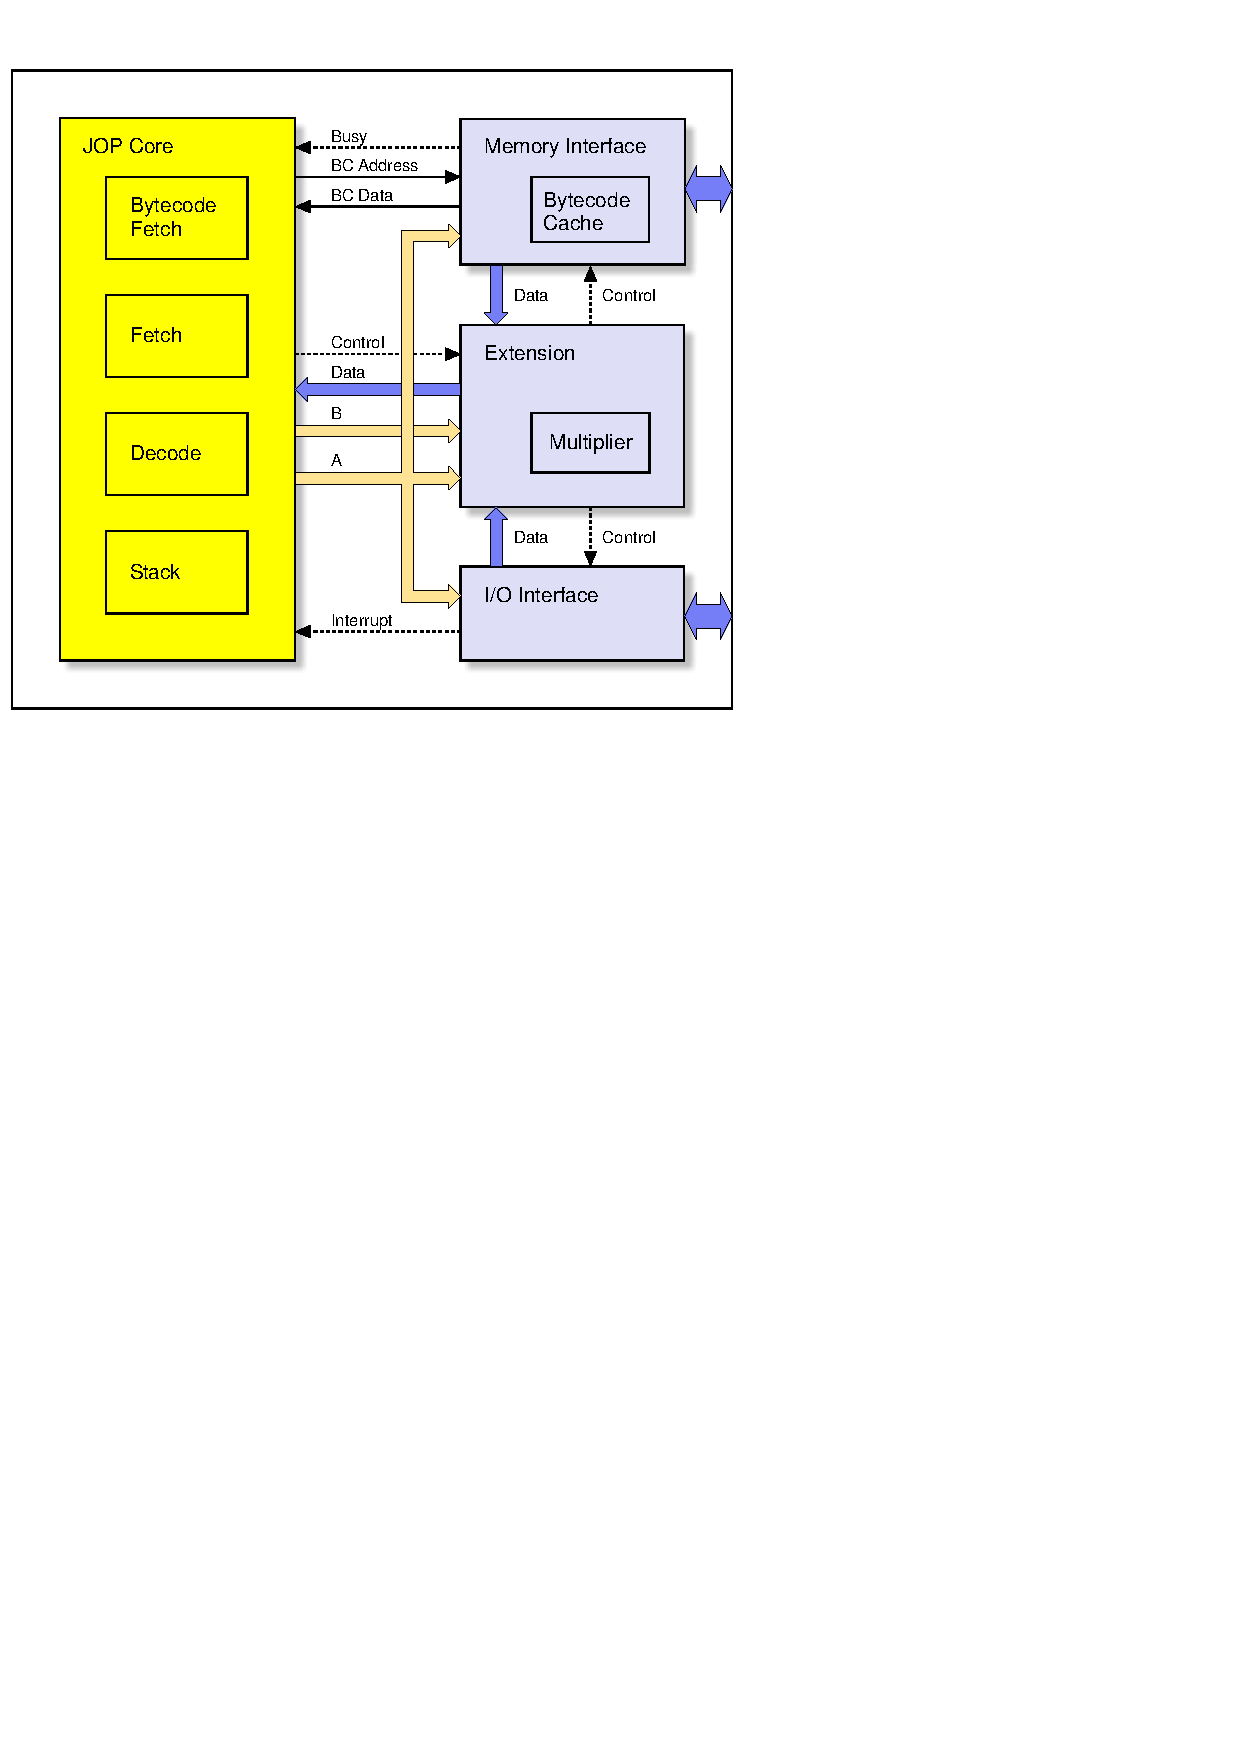
\includegraphics[scale=\picscale]{arch/arch_jop_block}
    \caption{Block diagram of JOP}
    \label{fig:arch:jop:block}
\end{figure}

The processor core contains the four pipeline stages \emph{bytecode
fetch}, \emph{microcode fetch}, \emph{decode} and \emph{execute}.
The ports to the other modules are the address and data bus for the
bytecode instructions, the two top elements of the stack (A and B),
input to the top-of-stack (Data) and a number of control signals.
There is no direct connection between the processor core and the
external world.

The memory interface provides a connection between the main memory
and the processor core. It also contains the bytecode cache. The
extension module controls data read and write. The \emph{busy}
signal is used by the microcode instruction \code{wait}\footnote{The
busy signal can also be used to stall the whole processor pipeline.
This was the change made to JOP by Flavius Gruian \cite{jop:sac05}.
However, in this synchronization mode, the concurrency between the
memory access module and the main pipeline is lost.} to synchronize
the processor core with the memory unit. The core reads bytecode
instructions through dedicated buses (BC address and BC data) from
the memory subsystem. The request for a method to be placed in the
cache is performed through the extension module, but the cache hit
detection and load is performed by the memory interface
independently of the processor core (and therefore concurrently).

The I/O interface contains peripheral devices, such as the system
time and timer interrupt, a serial interface and
application-specific devices. Read and write to and from this module
are controlled by the extension module. All external
devices\footnote{The external device can be as simple as a line
driver for the serial interface that forms part of the interface
module, or a complete bus interface, such as the ISA bus used to
connect e.g.\ an Ethernet chip.} are connected to the I/O interface.

The extension module performs three functions: (a) it contains
hardware accelerators (such as the multiplier unit in this example),
(b) the control for the memory and the I/O module, and (c) the
multiplexer for the read data that is loaded in the top-of-stack
register. The write data from the top-of-stack (A) is connected
directly to all modules.

The division of the processor into those four modules greatly
simplifies the adaptation of JOP for different application domains
or hardware platforms. Porting JOP to a new FPGA board usually
results in changes in the memory module alone. Using the same board
for different applications only involves making changes to the I/O
module. JOP has been ported to several different FPGAs and
prototyping boards and has been used in different applications (see
Chapter~\ref{chap:results}), but it never proved necessary to change
the processor core.

\section{Microcode}
\label{sec:microcode}

The following discussion concerns two different instruction sets:
\emph{bytecode} and \emph{microcode}. Bytecodes are the instructions
that make up a compiled Java program. These instructions are
executed by a Java virtual machine. The JVM does not assume any
particular implementation technology. Microcode is the native
instruction set for JOP. Bytecodes are translated, during their
execution, into JOP microcode. Both instruction sets are designed
for an extended\footnote{An extended stack machine is one in which
there are instructions available to access elements deeper down in
the stack.} stack machine.

\subsection{Translation of Bytecodes to Microcode}

To date, no hardware implementation of the JVM exists that is
capable of executing \emph{all} bytecodes in hardware alone. This is
due to the following: some bytecodes, such as \code{new}, which
creates and initializes a new object, are too complex to implement
in hardware. These bytecodes have to be emulated by software.

To build a self contained JVM without an underlying operating
system, direct access to the memory and I/O devices is necessary.
There are no bytecodes defined for low-level access. These low-level
services are usually implemented in \emph{native} functions, which
means that another language (C) is native to the processor. However,
for a Java processor, bytecode is the \emph{native} language.

One way to solve this problem is to implement simple bytecodes in
hardware and to emulate the more complex and \emph{native} functions
in software with a different instruction set (sometimes called
microcode). However, a processor with two different instruction sets
results in a complex design.

Another common solution, used in Sun's picoJava \cite{pjMicroArch},
is to execute a subset of the bytecode native and to use a software
trap to execute the remainder. This solution entails an overhead (a
minimum of 16 cycles in picoJava, see \ref{subsec:related:picojava})
for the software trap.

In JOP, this problem is solved in a much simpler way. JOP has a
single \emph{native} instruction set, the so-called microcode.
During execution, every Java bytecode is translated to either one,
or a sequence of microcode instructions. This translation merely
adds one pipeline stage to the core processor and results in no
execution overheads (except for a bytecode branch that takes 4
instead of 3 cycles to execute). The area overhead of the
translation stage is 290~LCs, or about 15\% of the LCs of a typical
JOP configuration. With this solution, we are free to define the JOP
instruction set to map smoothly to the stack architecture of the
JVM, and to find an instruction coding that can be implemented with
minimal hardware.

\begin{figure}
    \centering
    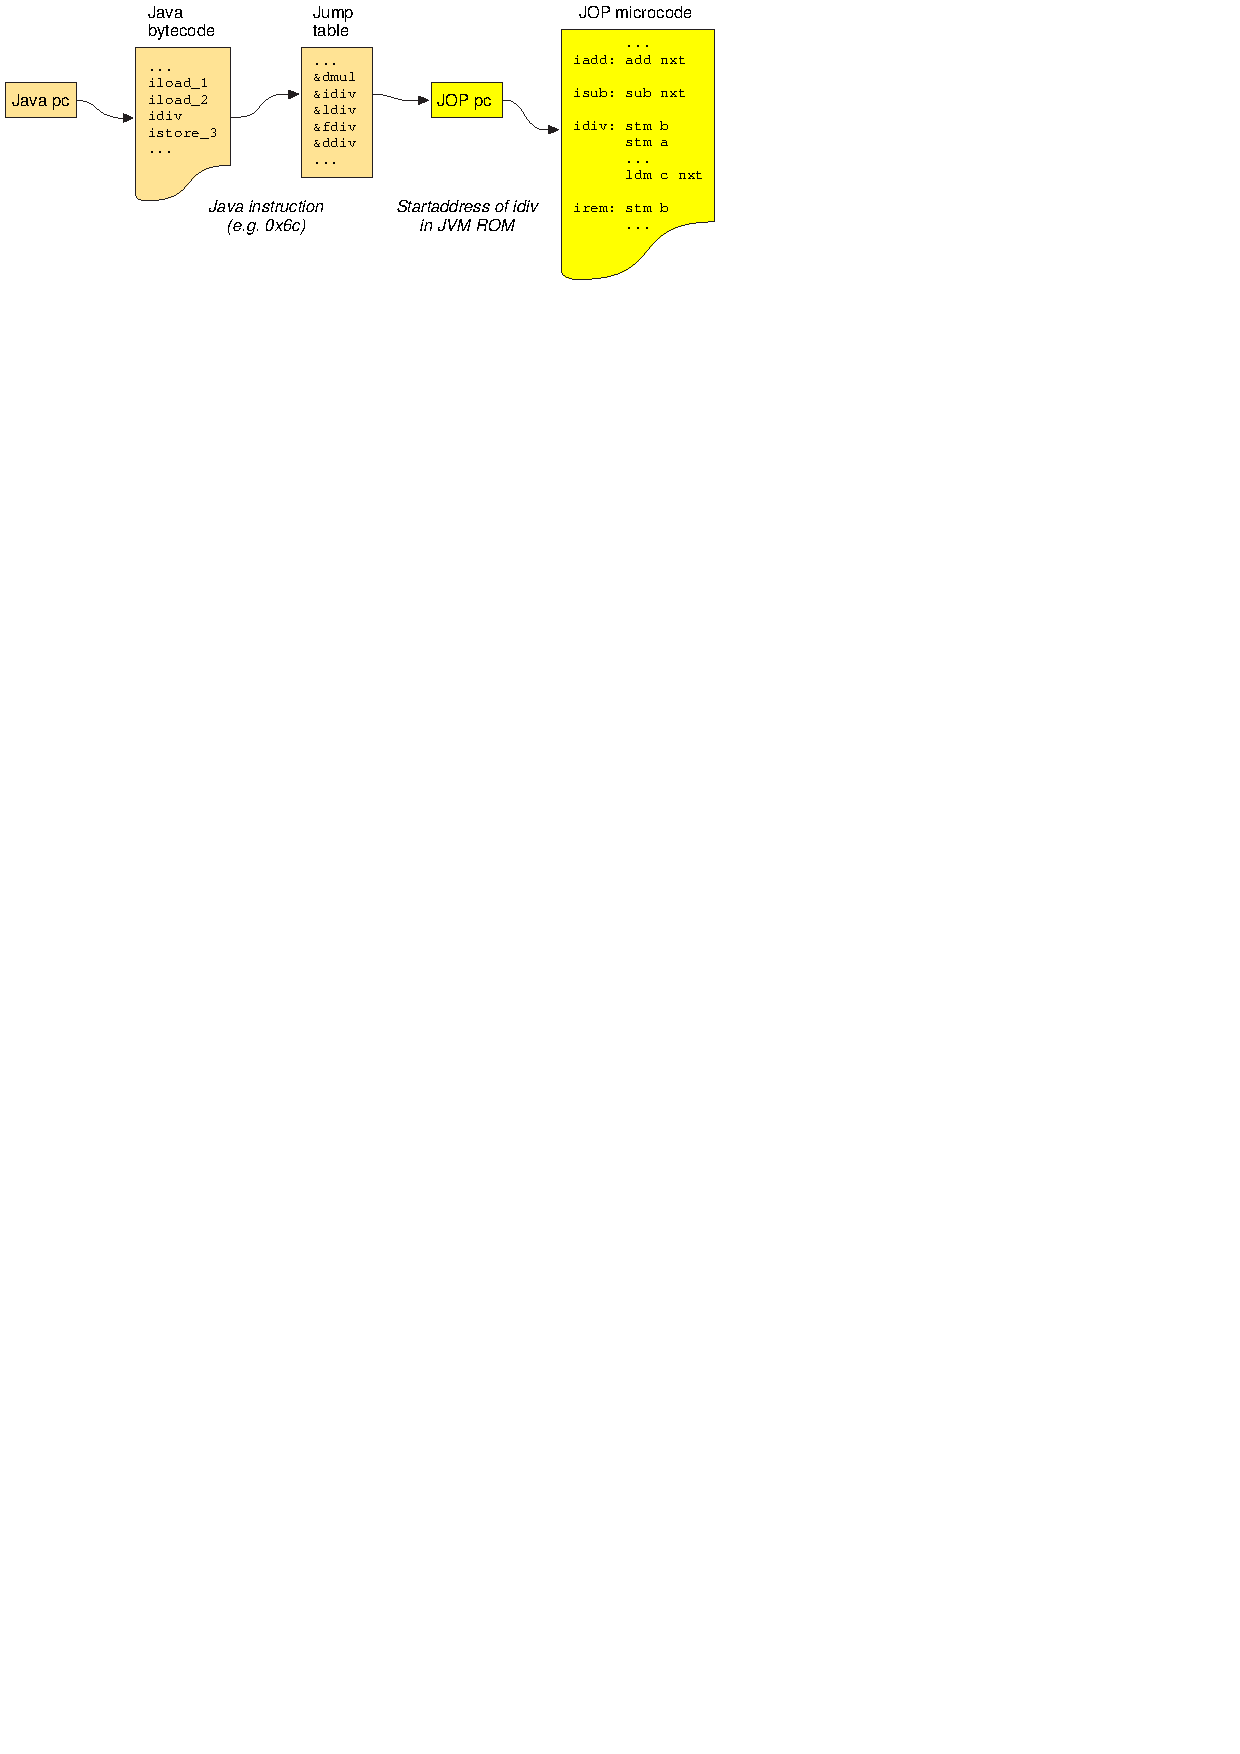
\includegraphics[scale=\picscale]{arch/arch_indirection}
    \caption{Data flow from the Java program counter to JOP microcode}
    \label{fig_arch_data_flow}
\end{figure}


Figure~\ref{fig_arch_data_flow} gives an example of the data flow
from the Java program counter to JOP microcode. The figure
represents the two pipeline stages bytecode fetch/translate and
microcode fetch. The fetched bytecode acts as an index for the jump
table. The jump table contains the start addresses for the bytecode
implementation in microcode. This address is loaded into the JOP
program counter for every bytecode executed. JOP executes the
sequence of microcode until the last one. The last one is marked
with \emph{nxt} in microcode assembler. This \emph{nxt} bit in the
microcode ROM triggers a new translation i.e., a new address is
loaded into the JOP program counter. In
Figure~\ref{fig_arch_data_flow} the implementation of bytecode
\code{idiv} is an example of a longer sequence that ends with
microcode instruction \code{ldm c nxt}.

The difference to other forms of instruction translation in hardware
is that the proposed solution is time predictable. The translation
takes one cycle (one pipeline stage) for each bytecode, independent
from the execution history. Instruction folding, e.g., implemented
in picoJava \cite{pJ1,pjMicroArch}, is also a form of instruction
translation in hardware. Folding is used to translate several (stack
oriented) bytecode instructions to a RISC type instruction. This
translation needs an instruction buffer and the fill level of this
instruction buffer depends on the execution history. The length of
this history that has to be considered for analysis is not bounded.
Therefore this form of instruction translation is not exactly time
predictable.


\subsection{Compact Microcode}

For the JVM to be implemented efficiently, the microcode has to
\emph{fit} to the Java bytecode. Since the JVM is a stack machine,
the microcode is also stack-oriented. However, the JVM is not a pure
stack machine. Method parameters and local variables are defined as
\emph{locals}. These locals can reside in a stack frame of the
method and are accessed with an offset relative to the start of this
\emph{locals} area.

Additional local variables (16) are available at the microcode
level. These variables serve as scratch variables, like registers in
a conventional CPU. However, arithmetic and logic operations are
performed on the stack.

Some bytecodes, such as ALU operations and the short form access to
\emph{locals}, are directly implemented by an equivalent microcode
instruction (with a different encoding). Additional instructions are
available to access internal registers, main memory and I/O devices.
A relative conditional branch (zero/non zero of TOS) performs
control flow decisions at the microcode level. For optimum use of
the available memory resources, all instructions are 8 bits long.
There are no variable-length instructions and every instruction,
with the exception of \code{wait}, is executed in a single cycle. To
keep the instruction set this dense, following concept is applied:
immediate values and branch offsets are addressed through one
indirection. The instruction just contains an index for the
constants.

Two types of operands, immediate values and branch distances,
normally force an instruction set to be longer than 8 bits. The
instruction set is either expanded to 16 or 32 bits, as in typical
RISC processors, or allowed to be of variable length at byte
boundaries. A first implementation of the JVM with a 16-bit
instruction set showed that only a small number of different
constants are necessary for immediate values and relative branch
distances.

In the current realization of JOP, the different immediate values
are collected while the microcode is being assembled and are put
into the initialization file for the on-chip memory. These constants
are accessed indirectly in the same way as the local variables. They
are similar to initialized variables, apart from the fact that there
are no operations to change their value during runtime, which would
serve no purpose and would waste instruction codes.  The microcode
local variables, the microcode constants and the stack share the
same on-chip memory. Using a single memory block simplifies the
multiplexer in the execution stage.

A similar solution is used for branch distances. The assembler
generates a VHDL file with a table for all found branch constants.
This table is indexed using instruction bits during runtime. These
indirections during runtime make it possible to retain an 8-bit
instruction set, and provide 16 different immediate values and 32
different branch constants. For a general purpose instruction set,
these indirections would impose too many restrictions. As the
microcode only implements the JVM, this solution is a viable option.

To simplify the logic for instruction decoding, the instruction
coding is carefully chosen. For example, one bit in the instruction
specifies whether the instruction will increment or decrement the
stack pointer. The offset to access the \emph{locals} is directly
encoded in the instruction. This is not the case for the original
encoding of the equivalent bytecodes (e.g. \emph{iload\_0} is 0x1a
and \emph{iload\_1} is 0x1b). Whenever a multiplexer depends on an
instruction, the selection is directly encoded in the instruction.

\subsection{Instruction Set}

JOP implements 45 different microcode instructions. These
instructions are encoded in 8 bits. With the addition of the
\emph{nxt} and \emph{opd} bits in every instruction, the effective
instruction length is 10 bits.

\begin{description}
    \item[Bytecode equivalent:]
These instructions are direct implementations of bytecodes and
result in one cycle execution time for the bytecode (except
\code{st} and \code{ld}): \code{pop}, \code{and}, \code{or},
\code{xor}, \code{add}, \code{sub}, \code{st$<$n$>$}, \code{st},
\code{ushr}, \code{shl}, \code{shr}, \code{nop}, \code{ld$<$n$>$},
\code{ld}, \code{dup}

    \item[Local memory access:]
The first 16 words in the internal stack memory are reserved for
internal variables. The next 16 words contain constants. These
memory locations are accessed using the following instructions:
\code{stm}, \code{stmi}, \code{ldm}, \code{ldmi}, \code{ldi}

    \item[Register manipulation:]
The stack pointer, the variable pointer and the Java program counter
are loaded or stored with: \code{stvp}, \code{stjpc}, \code{stsp},
\code{ldvp}, \code{ldjpc}, \code{ldsp}, \code{star}

    \item[Bytecode operand:]
The operand is loaded from the bytecode RAM, converted to a 32-bit
word and pushed on the stack with: \code{ld\_opd\_8s},
\code{ld\_opd\_8u}, \code{ld\_opd\_16s}, \code{ld\_opd\_16u}

    \item[External memory access:]
The autonomous memory subsystem and the IO subsystem are accessed by
using the following instructions: \code{stmra}, \code{stmwa},
\code{stmwd}, \code{wait}, \code{ldmrd}, \code{stbcrd},
\code{ldbcstart}, \code{stald}, \code{stast},

    \item[Multiplier:]
The multiplier is accessed with: \code{stmul}, \code{ldmul}

    \item[Microcode branches:]
Two conditional branches in microcode are available: \code{bz},
\code{bnz}

    \item[Bytecode branch:]
All 17 bytecode branch instructions are mapped to one instruction:
\code{jbr}

\end{description}
%
A detailed description of the microcode instructions can be found in
Appendix~\ref{appx:jop:instr}.

\subsection{Bytecode Example}

The example in Figure~\ref{lst:arch:micro1} shows the implementation
of a single cycle bytecode and an infrequent bytecode as a sequence
of JOP instructions. The suffix \code{nxt} marks the last
instruction of the microcode sequence. In this example, the
\code{dup} bytecode is mapped to the equivalent \code{dup} microcode
and executed in a single cycle, whereas \code{dup\_x1} takes five
cycles to execute, and after the last instruction (\code{ldm a
nxt}), the first instruction for the next bytecode is executed. The
scratch variables, as shown in the second example, are stored in the
on-chip memory that is shared with the stack cache.

\begin{lstlisting}[caption={Implementation of \code{dup} and \code{dup\_x1}},
label=lst:arch:micro1]
    dup:    dup nxt    // 1 to 1 mapping

    //  a and b are scratch variables for the
    //  JVM code.
    dup_x1: stm a      // save TOS
            stm b      // and TOS-1
            ldm a      // duplicate former TOS
            ldm b      // restore TOS-1
            ldm a nxt  // restore TOS and fetch next bytecode
\end{lstlisting}

Some bytecodes are followed by operands of between one and three
bytes in length (except \code{lookupswitch} and \code{tableswitch}).
Due to pipelining, the first operand byte that follows the bytecode
instruction is available when the first microcode instruction enters
the execution stage. If this is a one-byte long operand, it is ready
to be accessed. The increment of the Java program counter after the
read of an operand byte is coded in the JOP instruction (an
\emph{opd} bit similar to the \emph{nxt} bit).

In Listing~\ref{lst:arch:micro2}, the implementation of
\code{sipush} is shown. The bytecode is followed by a two-byte
operand. Since the access to bytecode memory is only
one\footnote{The decision is to avoid buffers that would introduce
time dependencies over bytecode boundaries.} byte per cycle,
\emph{opd} and \emph{nxt} are not allowed at the same time. This
implies a minimum execution time of $n+1$ cycles for a bytecode with
$n$ operand bytes.

\begin{lstlisting}[caption={Bytecode operand load},
label=lst:arch:micro2]
    sipush: nop opd        // fetch next byte
            nop opd        // and one more
            ld_opd_16s nxt // load 16 bit operand
\end{lstlisting}


\subsection{Flexible Implementation of Bytecodes}
\label{subsec:flex:bc}

As mentioned above, some Java bytecodes are very complex. One
solution already described is to emulate them through a sequence of
microcode instructions. However, some of the more complex bytecodes
are very seldom used. To further reduce the resource implications
for JOP, in this case local memory, bytecodes can even be
implemented by \emph{using} Java bytecodes. That means bytecodes
(e.g., \code{new} or floating point operations) can be implemented
in Java. This feature also allows for the easy configuration of
resource usage versus performance.

During the assembly of the JVM, all labels that represent an entry
point for the bytecode implementation are used to generate the
translation table. For all bytecodes for which no such label is
found, i.e.\ there is no implementation in microcode, a
\emph{not-implemented} address is generated. The instruction
sequence at this address invokes a static method from a system
class. This class contains 256 static methods, one for each possible
bytecode, ordered by the bytecode value. The bytecode is used as the
index in the method table of this system class. A single empty
static method consumes three 32-bit words in memory. Therefore, the
overhead of this special class is 3~KB, which is 9\% of a minimal
\emph{hello world} program (34~KB memory footprint). As described in
Section~\ref{sec:hwsw:co}, this feature also allows for the easy
configuration of resource usage versus performance.

\subsection{Summary}

In order to handle the great variation in the complexity of Java
bytecodes we have proposed a translation to a different instruction
set, the so-called microcode. This microcode is still an instruction
set for a stack machine, but more RISC-like than the CISC-like JVM
bytecodes.

At the time of this writing 43 of the 201 different bytecodes are
implemented by a single microcode instruction, 93 by a microcode
sequence, and 40 bytecodes are implemented in Java. In the next
section we will see how this translation is handled in JOP's
pipeline and how it can simplify interrupt handling.


\section{The Processor Pipeline}
\label{sec:pipeline}

JOP is a fully pipelined architecture with single cycle execution of
microcode instructions and a novel approach of translation from Java
bytecode to these instructions. Figure~\ref{fig_arch_pipeline} shows
the datapath for JOP, representing the pipeline from left to right.
Blocks arranged vertically belong to the same pipeline stage.

\begin{figure}
    \centering
    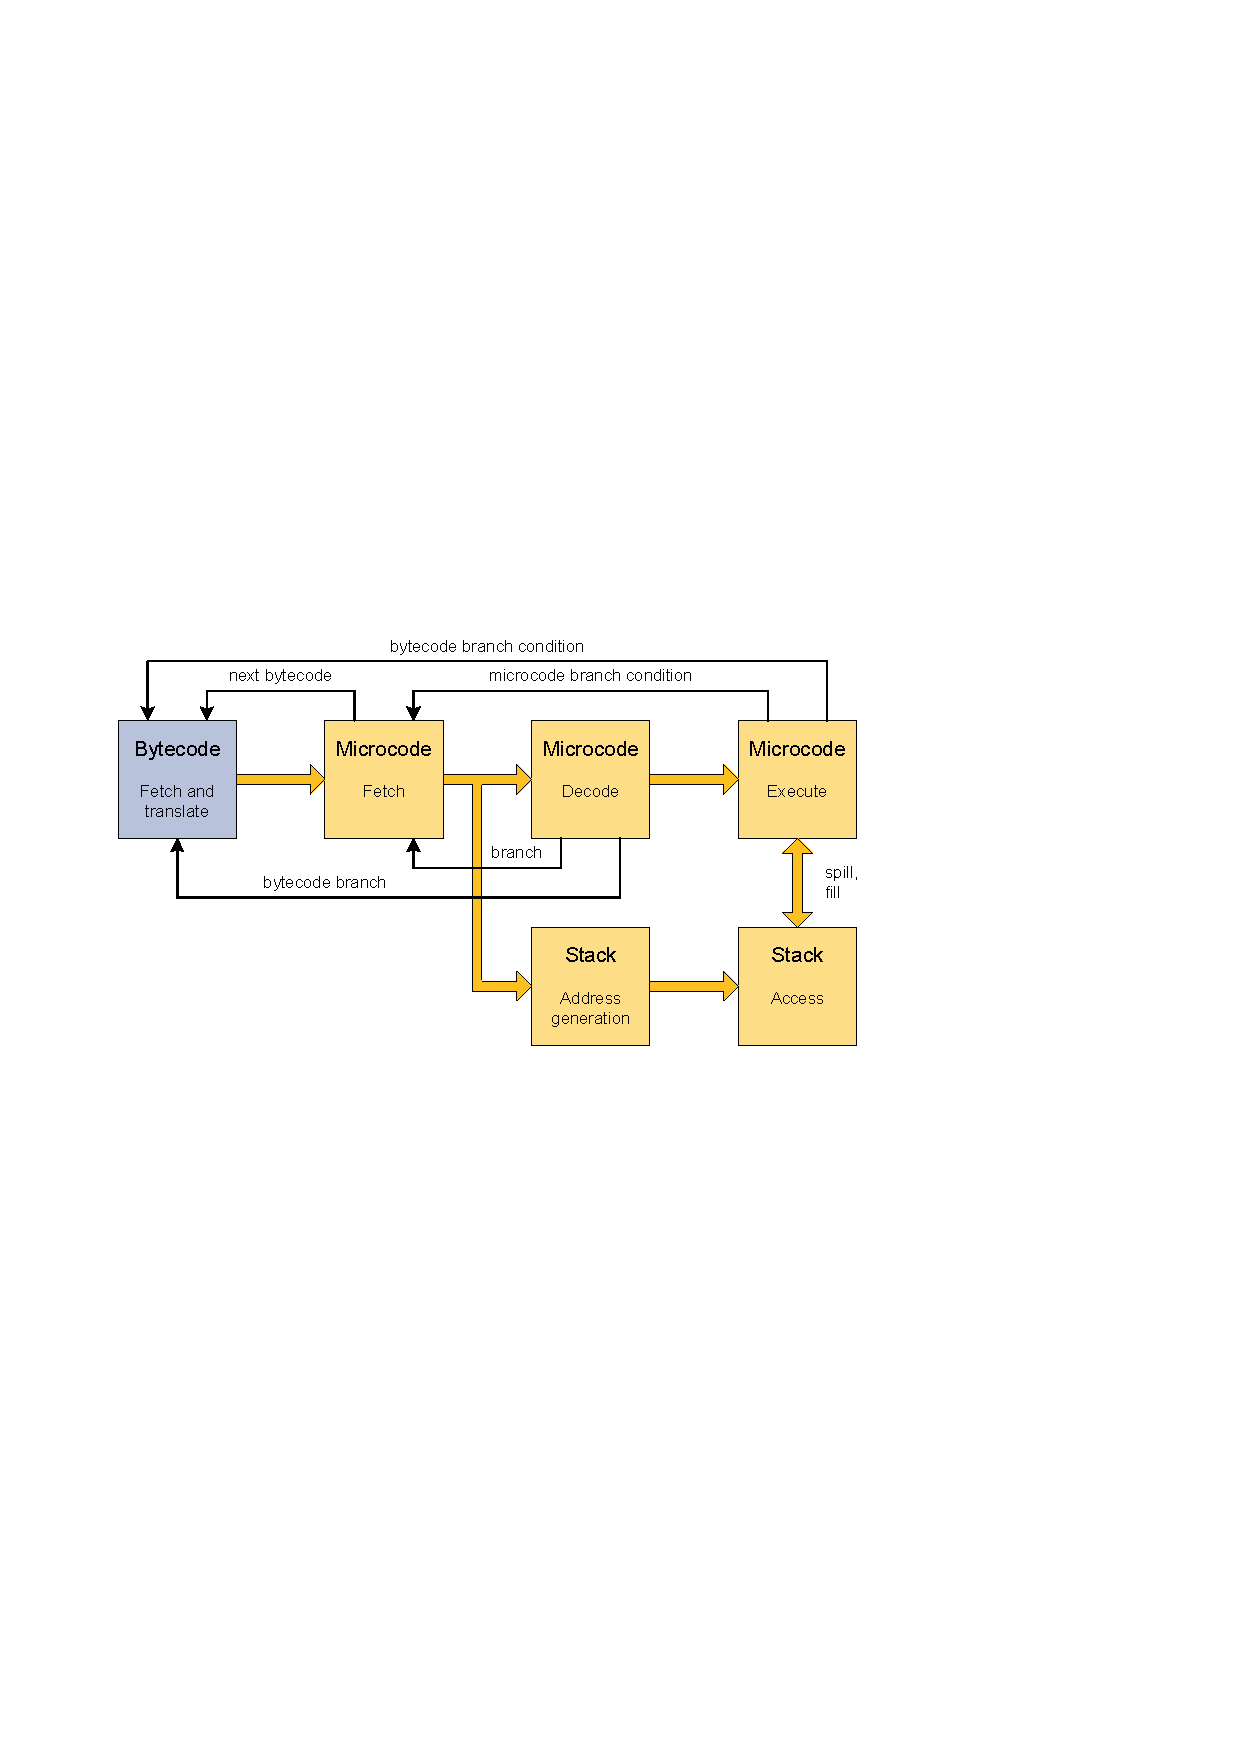
\includegraphics[scale=\picscale]{arch/arch_pipeline}
    \caption{Datapath of JOP}
    \label{fig_arch_pipeline}
\end{figure}

Three stages form the JOP core pipeline, executing microcode
instructions. An additional stage in the front of the core pipeline
fetches Java bytecodes -- the instructions of the JVM -- and
translates these bytecodes into addresses in microcode. Bytecode
branches are also decoded and executed in this stage. The second
pipeline stage fetches JOP instructions from the internal microcode
memory and executes microcode branches. Besides the usual decode
function, the third pipeline stage also generates addresses for the
stack RAM (the stack cache). As every stack machine microcode
instruction (except \code{nop}, \code{wait}, and \code{jbr}) has
either \emph{pop} or \emph{push} characteristics, it is possible to
generate fill or spill addresses for the \emph{following}
instruction at this stage. The last pipeline stage performs ALU
operations, load, store and stack spill or fill. At the execution
stage, operations are performed with the two topmost elements of the
stack.

The stack architecture allows for a short pipeline, which results in
short branch delays. Two branch delay slots are available after a
conditional microcode branch. A stack machine with two explicit
registers for the two topmost stack elements and automatic
fill/spill to the stack cache needs neither an extra write-back
stage nor any data forwarding. See Section~\ref{sec:stack} for a
detailed description.

The method cache (\emph{Bytecode Cache}), microcode ROM, and stack
RAM are implemented with single cycle access in the FPGA's internal
memories.


\subsection{Java Bytecode Fetch}

In the first pipeline stage, as shown in
Figure~\ref{fig_arch_bc_fetch}, the Java bytecodes are fetched from
the internal memory (\emph{Bytecode RAM}). The bytecode is mapped
through the translation table into the address (\emph{jpaddr}) for
the microcode ROM.

\begin{figure}
    \centering
    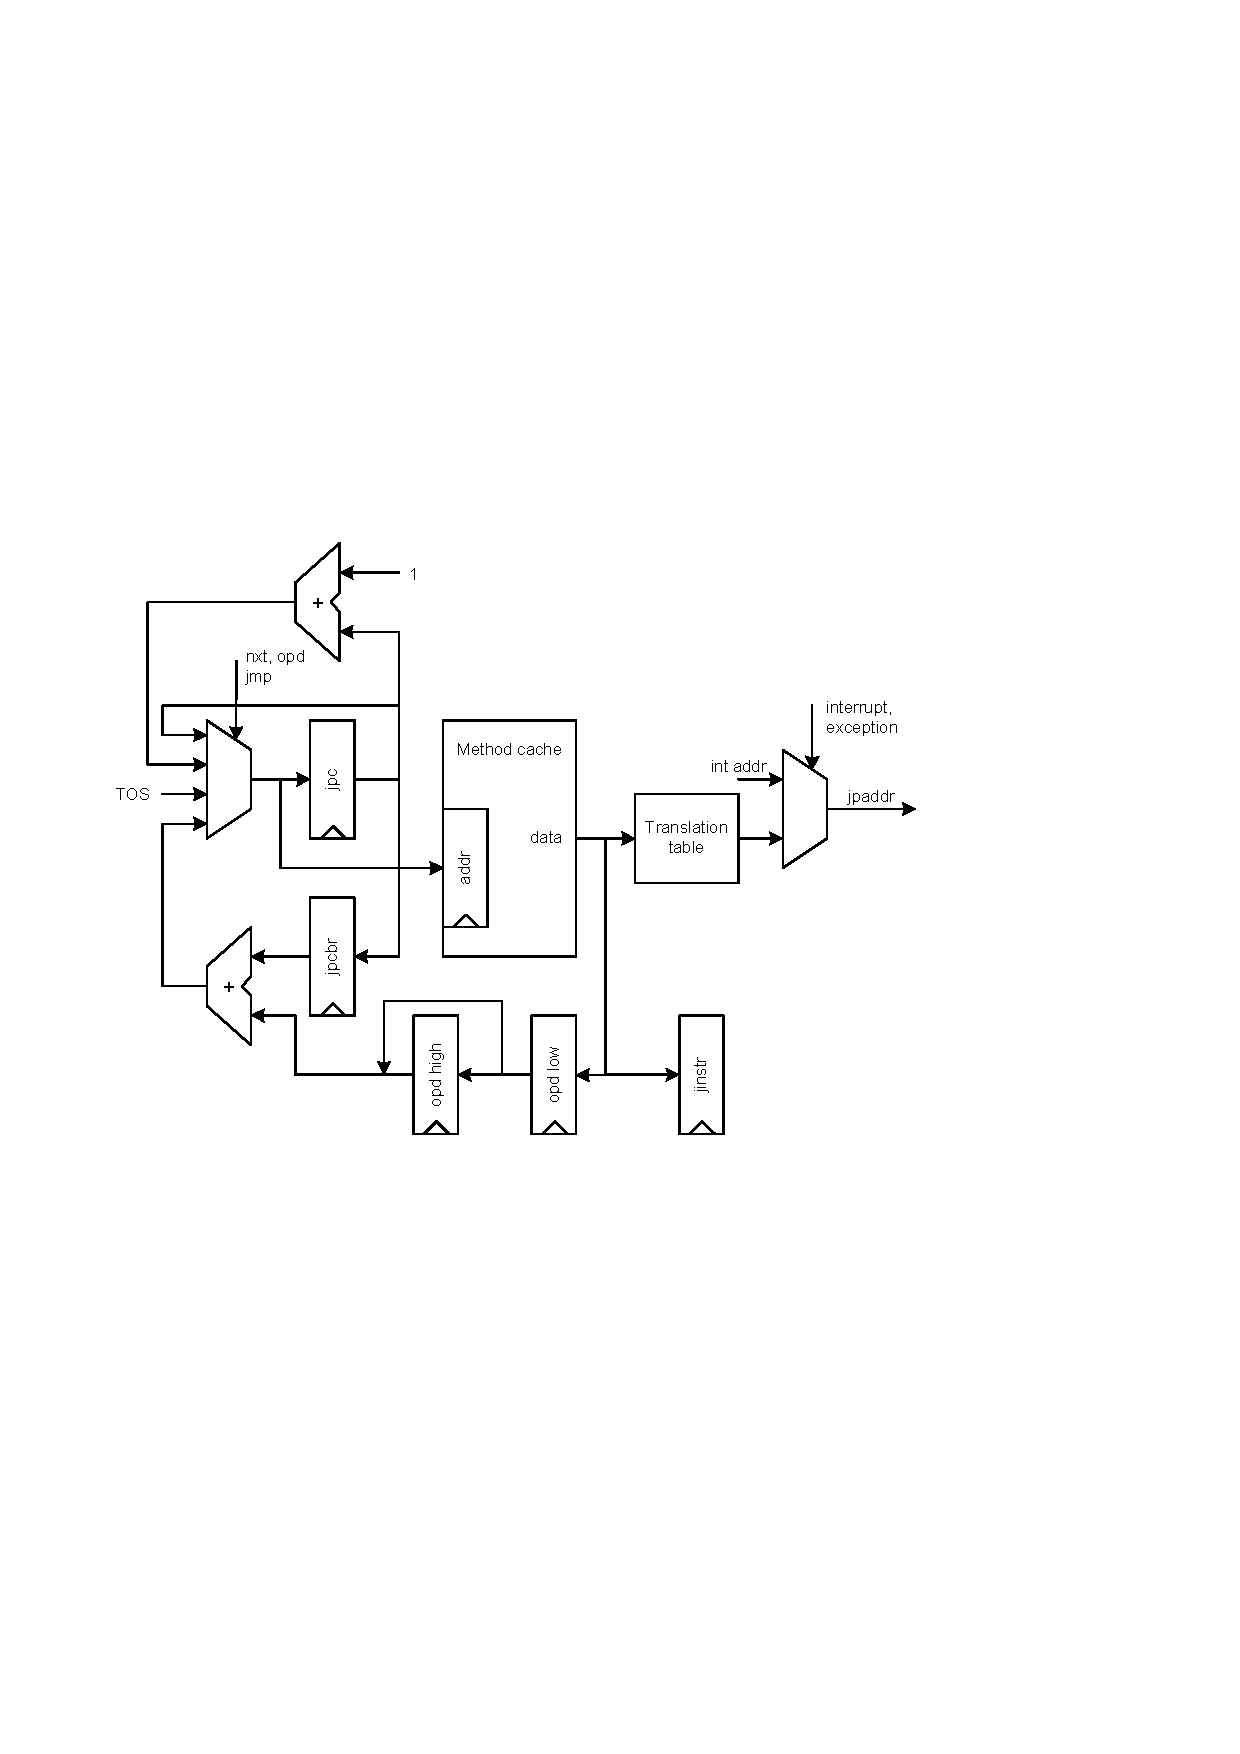
\includegraphics[scale=\picscale]{arch/arch_bcfetch}
    \caption{Java bytecode fetch}
    \label{fig_arch_bc_fetch}
\end{figure}

The fetched bytecode results in an absolute jump in the microcode
(the second stage). If the bytecode is mapped one-to-one with a JOP
instruction, the following fetched bytecode again results in a jump
in the microcode in the following cycle. If the bytecode is a
complex one, JOP continues to execute microcode. At the end of this
instruction sequence the next bytecode, and therefore the new jump
address, is requested (signal \emph{nxt}).

The bytecode RAM serves as instruction cache and is filled on method
invoke and return. Details about this time-predictable instruction
cache can be found in Section~\ref{sec:cache}.

The bytecode is also stored in a register for later use as an
operand (requested by signal \emph{opd}). Bytecode branches are also
decoded and executed in this stage. Since \emph{jpc} is also used to
read the operands, the program counter is saved in \emph{jpcbr}
during an instruction fetch. \emph{jinstr} is used to decode the
branch type and \emph{jpcbr} to calculate the branch target address.

\subsection{JOP Instruction Fetch}

The second pipeline stage, as shown in Figure~\ref{fig_arch_fetch},
fetches JOP instructions from the internal microcode memory and
executes microcode branches.

\begin{figure}
    \centering
    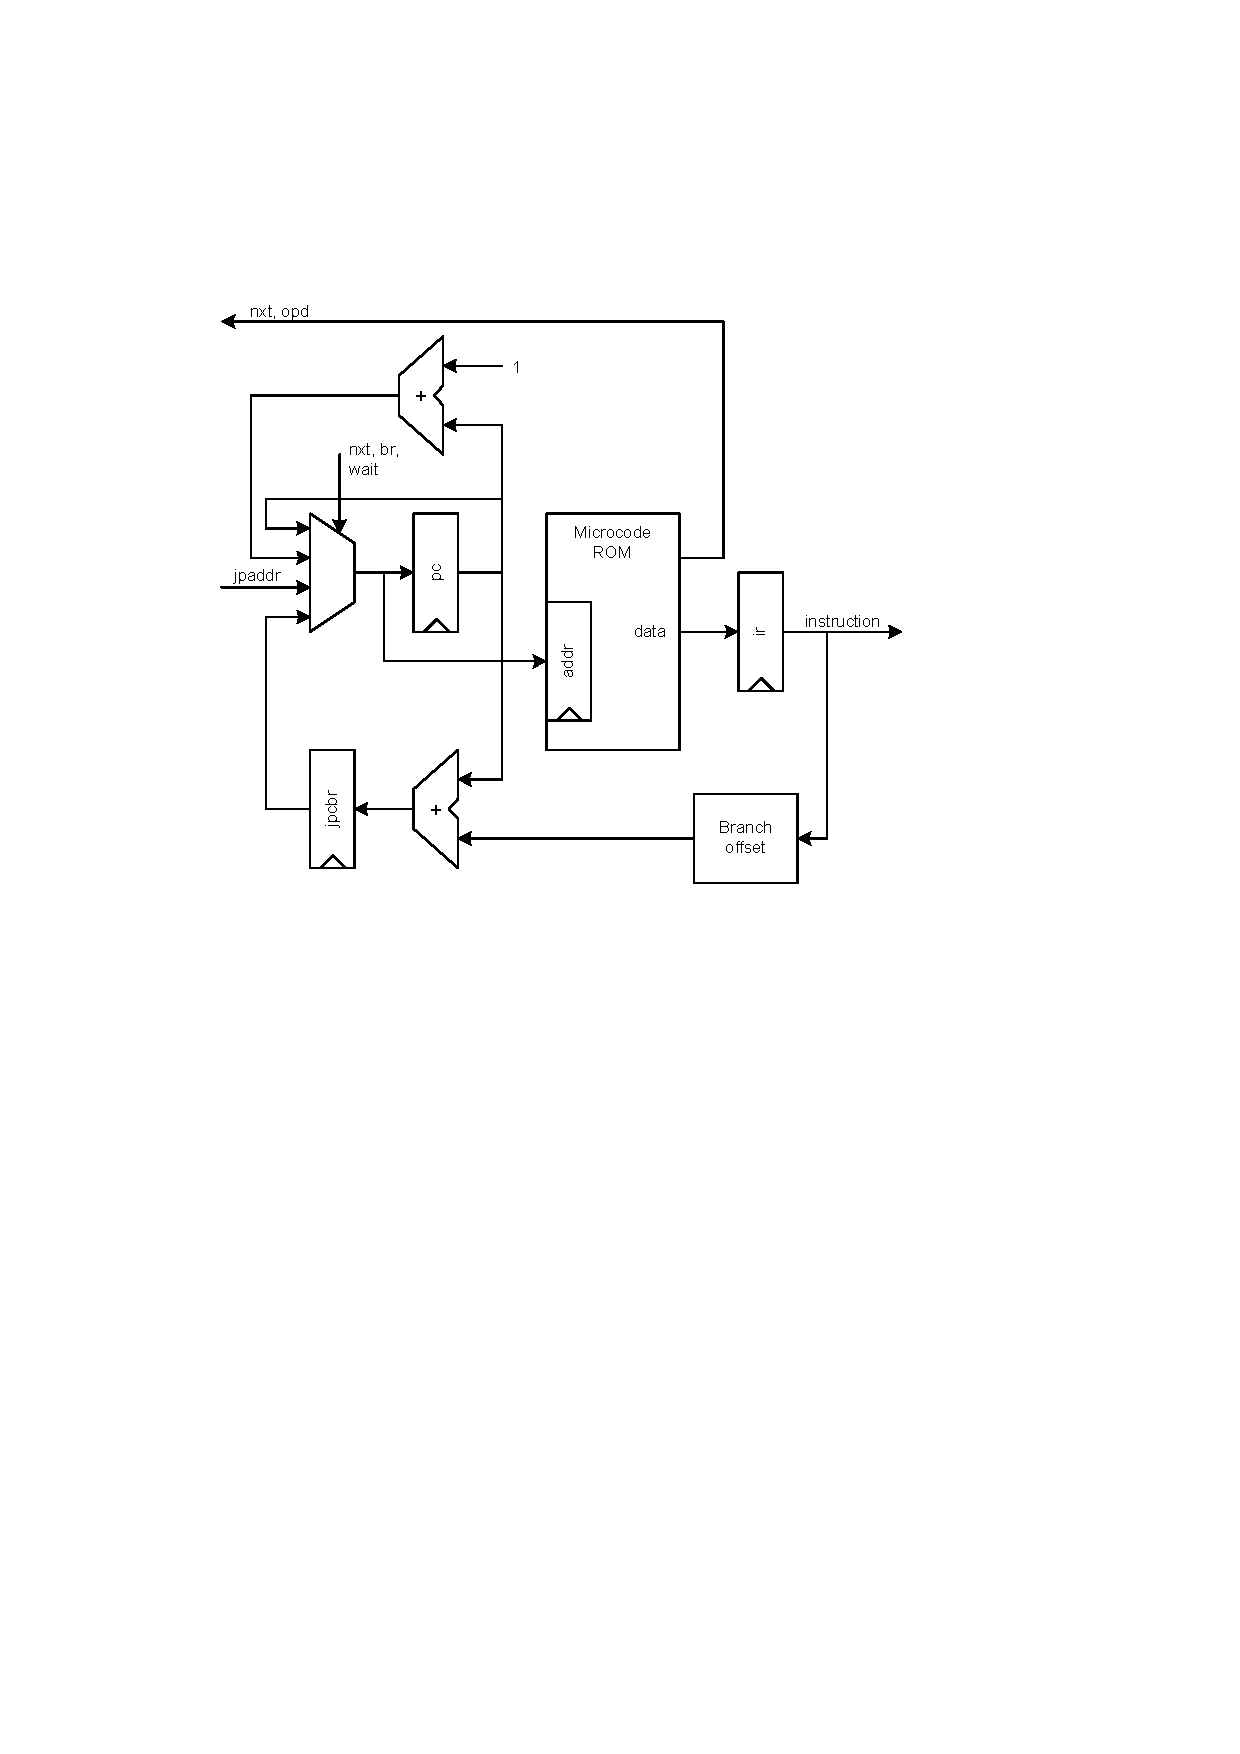
\includegraphics[scale=\picscale]{arch/arch_fetch}
    \caption{JOP instruction fetch}
    \label{fig_arch_fetch}
\end{figure}

The JOP microcode, which implements the JVM, is stored in the
microcode ROM. The program counter \emph{pc} is incremented during
normal execution. If the instruction is labeled with \emph{nxt} a
new bytecode is requested from the first stage and \emph{pc} is
loaded with \emph{jpaddr}. \emph{jpaddr} is the starting address for
the implementation of that bytecode. The label \emph{nxt} is the
flag that marks the end of the microcode instruction stream for one
bytecode. Another flag, \emph{opd}, indicates that a bytecode
operand needs to be fetched in the first pipeline stage. Both flags
are stored in a table that is indexed by the program counter.

\emph{brdly} contains the target address for a conditional branch.
The same offset is shared by a number of branch destinations. A
table (\emph{branch offset}) is used to store these relative
offsets. This indirection means that only 5 bits need to be used in
the instruction coding for branch targets and thereby allow greater
offsets. The three tables \emph{BC fetch table}, \emph{branch
offset} and \emph{translation table} (from the bytecode fetch stage)
are generated during the assembly of the JVM code. The outputs are
plain VHDL files. For an implementation in an FPGA, recompiling the
design after changing the JVM implementation is a straightforward
operation. For an ASIC with a loadable JVM, it is necessary to
implement a different solution.

FPGAs available to date do not allow asynchronous memory access.
They therefore force us to use the registers in the memory blocks.
However, the output of these registers is not accessible. To avoid
having to create an additional pipeline stage just for a
register-register move, the read address register of the microcode
ROM is clocked on the negative edge.

An alternative solution for this problem would be to use the output
of the multiplexer for the \emph{pc} and the read address register
of the memory. However, this solution results in a longer critical
path, as the multiplexer can no longer be combined with the
flip-flops that form the \emph{pc} in the same LCs. This is an
example of how implementation technology (the FPGA) can influence
the architecture.

\subsection{Decode and Address Generation}

Besides the usual decode function, the third pipeline, as shown in
Figure~\ref{fig_arch_decode}, also generates addresses for the stack
RAM.

\begin{figure}
    \centering
    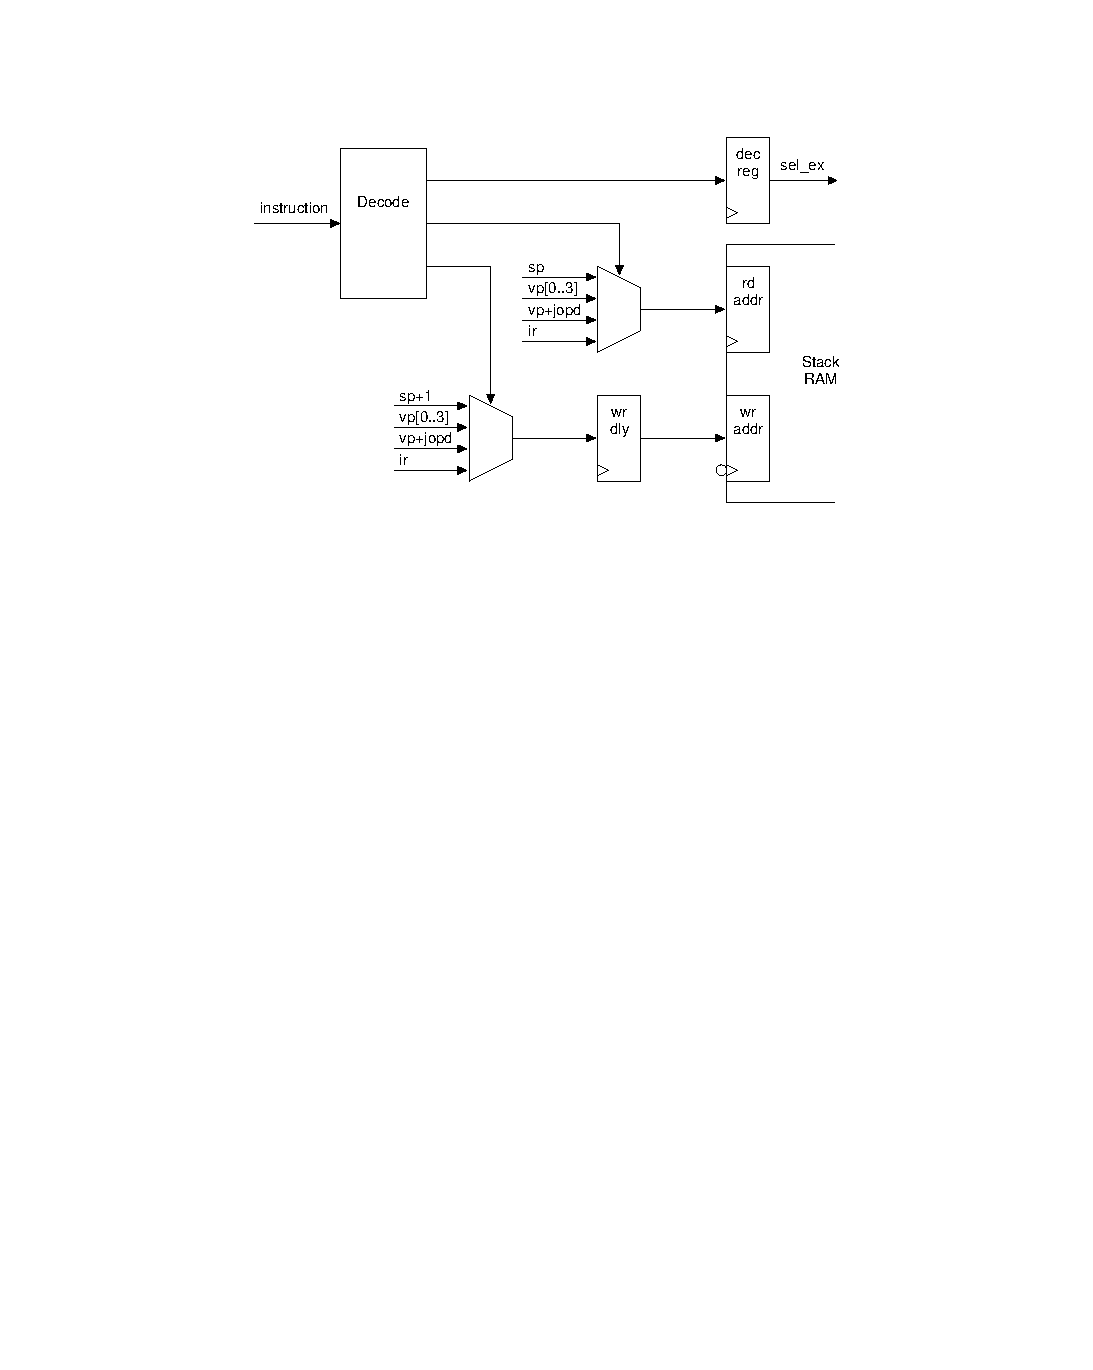
\includegraphics[scale=\picscale]{arch/arch_decaddr}
    \caption{Decode and address generation}
    \label{fig_arch_decode}
\end{figure}


As we can see in Section~\ref{sec:stack}
Table~\ref{tab_stack_address}, read and write addresses are either
relative to the stack pointer or to the variable pointer. The
selection of the pre-calculated address can be performed in the
decode stage. When an address relative to the stack pointer is used
(either as read or as write address, never for both) the stack
pointer is also decremented or incremented in the decode stage.

Stack machine instructions can be categorized from a stack
manipulation perspective as either \emph{pop} or \emph{push}. This
allows us to generate fill or spill TOS-1 addresses for the
\emph{following} instruction during the decode stage, thereby saving
one extra pipeline stage.

\subsection{Execute}

At the execution stage, as shown in Figure~\ref{fig_arch_exe},
operations are performed using two discrete registers: TOS and
TOS-1, labeled \emph{A} and \emph{B}.

\begin{figure}
    \centering
    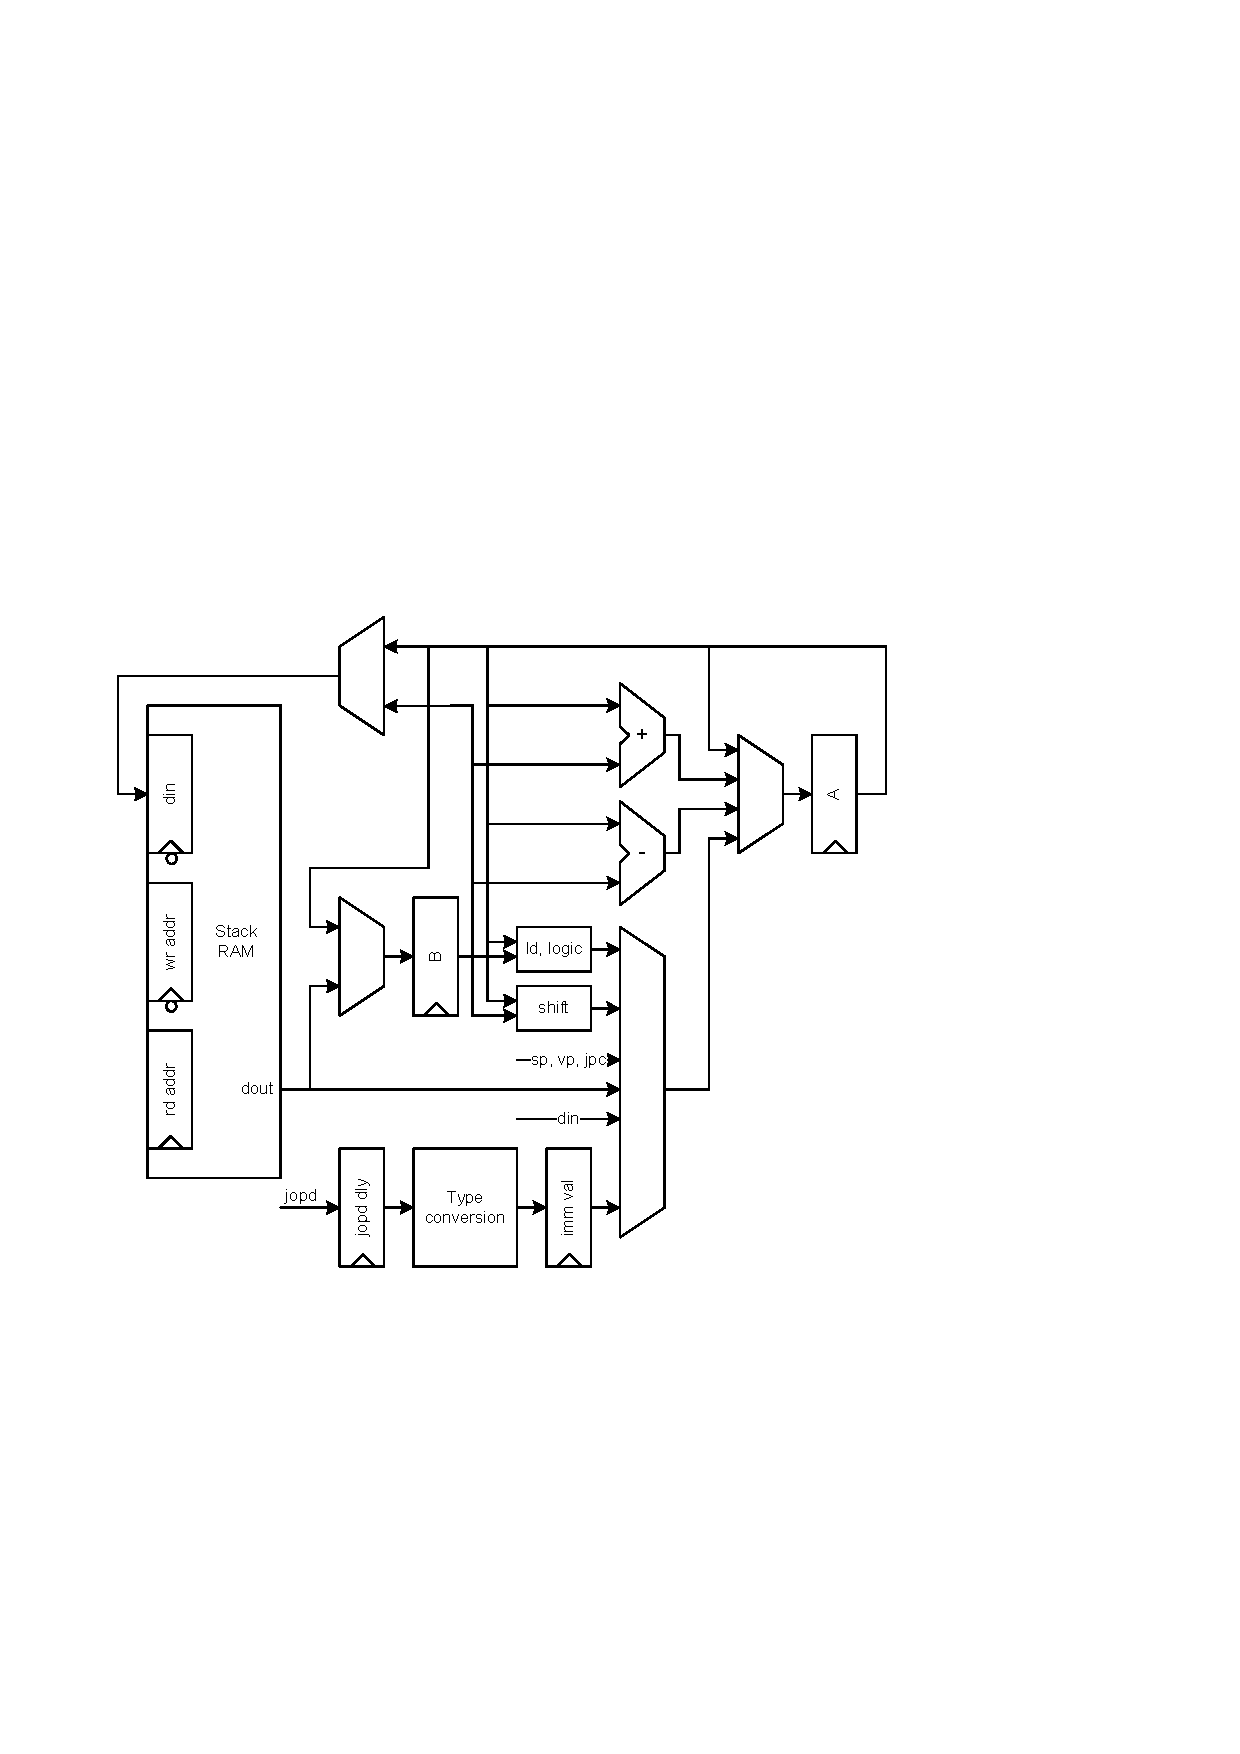
\includegraphics[scale=\picscale]{arch/arch_execute}
    \caption{Execution stage}
    \label{fig_arch_exe}
\end{figure}

Each arithmetic/logical operation is performed with registers
\emph{A} and \emph{B} as the source, and register \emph{A} as the
destination. All load operations (local variables, internal
register, external memory and periphery) result in a value being
loaded into register \emph{A}. There is therefore no need for a
write-back pipeline stage. Register \emph{A} is also the source for
the store operations. Register \emph{B} is never accessed directly.
It is read as an implicit operand or for stack spill on push
instructions. It is written during the stack spill with the content
of the stack RAM or the stack fill with the content of register
\emph{A}.

Beside the Java stack, the stack RAM also contains microcode
variables and constants. This resource-sharing arrangement not only
reduces the number of memory blocks needed for the processor, but
also the number of data paths to and from the register \nolinebreak
\emph{A}.

The inverted clock on data-in and on the write address register of
the stack RAM is used, for the same reason, as on the read address
register of the microcode ROM.

A stack machine with two explicit registers for the two topmost
stack elements and automatic fill/spill needs neither an extra
write-back stage nor any data forwarding. Details of this two-level
stack architecture are described in Section~\ref{sec:stack}.

%\subsection{Pipeline Example}
%
%\emph{\textbf{Show from Java code downto FPGA HW.}}
%
%Is in brown bock.

\subsection{Interrupt Logic}
\label{sec:interrupt}

Interrupts and (precise) exceptions are considered hard to implement
in a pipelined processor \cite{Hennessy02}, meaning implementation
tends to be complex (and therefore resource consuming). In JOP, the
bytecode-microcode translation is used cleverly to avoid having to
handle interrupts and exceptions (e.g., stack overflow) in the core
pipeline.

Interrupts are implemented as special bytecodes. These bytecodes are
inserted by the hardware in the Java instruction stream. When an
interrupt is pending and the next fetched byte from the bytecode
cache is an instruction (as indicated by the \emph{nxt} bit in the
microcode), the associated special bytecode is used instead of the
instruction from the bytecode cache. The result is that interrupts
are accepted at bytecode boundaries. The worst-case preemption delay
is the execution time of the \emph{slowest} bytecode that is
implemented in microcode. Bytecodes that are implemented in Java
(see Section \ref{subsec:flex:bc}) can be interrupted.

The implementation of interrupts at the bytecode-microcode mapping
stage keeps interrupts transparent in the core pipeline and avoids
complex logic. Interrupt handlers can be implemented in the same way
as standard bytecodes are implemented i.e.\ in microcode or Java.

This special bytecode can result in a call of a JVM internal method
in the context of the interrupted thread. This mechanism implicitly
stores almost the complete context of the current active thread on
the stack. This feature is used to implement the preemptive, fixed
priority real-time scheduler in Java \cite{jop:javasched}.

The main source for an interrupt is the $\mu$s accurate timer
interrupt used by the real-time scheduler. Hardware generated
exceptions, such as stack overflow or array bounds checks, generate
a system interrupt. The exception reason can be found in a register.

\subsection{Summary}

In this section, we have analyzed JOP's pipeline. The core of the
stack machine constitutes a three-stage pipeline. In the following
section, we will see that this organization is an optimal solution
for the stack access pattern of the JVM.

An additional pipeline stage in front of this core pipeline stage
performs bytecode fetch and the translation to microcode. This
organization has zero overheads for more complex bytecodes and
results in the short pipeline that is necessary for any processor
without branch prediction. This additional translation stage also
presents an elegant way of incorporating interrupts virtually
\emph{for free}.


\clearpage
    \section{An Efficient Stack Machine}
    \label{sec:stack}
    
The concept of a stack has a long tradition, but stack machines no
longer form part of mainstream computers. Although stacks are no
longer used for expression evaluation, they are still used for the
context save on a function call. A niche language, Forth
\cite{Koopman89}, is stack-based and known as an efficient language
for controller applications. Some hardware implementations of the
Forth abstract machine do exist. These Forth processors are stack
machines.

The Java programming language defines not only the language but also
a binary representation of the program and an abstract machine, the
JVM, to execute this binary. The JVM is similar to the Forth
abstract machine in that it is also a stack machine. However, the
usage of the stack differs from Forth in such a way that a Forth
processor is not an ideal hardware platform to execute Java
programs.

In this section, the stack usage in the JVM is analyzed. We will see
that, besides the access to the top elements of the stack, an
additional access path to an arbitrary element of the stack is
necessary for an efficient implementation of the JVM. Two
architectures will be presented for this mixed access mode of the
stack. Both architectures are used in Java processors. However, we
will also show that the JVM does not need a full three-port access
to the stack as implemented in the two architectures. This allows
for a simple and more elegant design of the stack for a Java
processor. This proposed architecture will then be compared with the
other two at the end of this section.

\subsection{Java Computing Model}

The JVM is not a pure stack machine in the sense of, for instance,
the stack model in Forth. The JVM operates on a LIFO stack as its
\emph{operand stack}. The JVM supplies instructions to load values
on the operand stack, and other instructions take their operands
from the stack, operate on them and push the result back onto the
stack. For example, the \code{iadd} instruction pops two values from
the stack and pushes the result back onto the stack. These
instructions are the stack machine's typical zero-address
instructions. The maximum depth of this operand stack is known at
compile time. In typical Java programs, the maximum depth is very
small. To illustrate the operation notation of the JVM,
Table~\ref{tab_stack_not} shows the evaluation of an expression for
a stack machine notation and the JVM bytecodes. Instruction
\code{iload{\_}n} loads an integer value from a local variable at
position \emph{n} and pushes the value on TOS.

\begin{table}[htbp]
    \centering
    \begin{tabular}{ll}
        \toprule
        \multicolumn{2}{c}{\emph{A = B + C * D}}  \\
        \midrule
        Stack & JVM \\
        \midrule
        push B& iload{\_}1 \\
        push C& iload{\_}2 \\
        push D& iload{\_}3 \\
        {*}   & imul \\
        +     & iadd \\
        pop A & istore{\_}0 \\
        \bottomrule
    \end{tabular}
    \caption{Standard stack notation and the corresponding
    JVM instructions}
    \label{tab_stack_not}
\end{table}

The JVM contains another memory area for method local data. This
area is known as \emph{local variables}. Primitive type values, such
as integer and float, and references to objects are stored in these
local variables. Arrays and objects cannot be allocated in a local
variable, as in C/C++. They have to be placed on the heap. Different
instructions transfer data between the operand stack and the local
variables. Access to the first four elements is optimized with
dedicated single byte instructions, while up to 256 local variables
are accessed with a two-byte instruction and, with the \code{wide}
modifier, the area can contain up to 65536 values.

These local variables are very similar to registers and it appears
that some of these locals can be mapped to the registers of a
general purpose CPU or implemented as registers in a Java processor.
On method invocation, local variables could be saved in a frame on a
stack, different from the operand stack, together with the return
address, in much the same way as in C on a typical processor. This
would result in the following memory hierarchy:
%
\begin{itemize}
\item On-chip hardware stack for ALU operations
\item A small register file for frequently-accessed variables
\item A method stack in main memory containing the return address and additional
local variables
\end{itemize}
%
However, the semantics of method invocation suggest a different
model. The arguments of a method are pushed on the operand stack. In
the invoked method, these arguments are not on the operand stack but
are instead accessed as the first variables in the local variable
area. The \emph{real} method local variables are placed at higher
indices. Listing~\ref{lst:stack:param:pass} gives an example of the
argument passing mechanism in the JVM. These arguments could be
copied to the local variable area of the invoked method. To avoid
this memory transfer, the entire variable area (the arguments
\emph{and} the variables of the method) is allocated on the operand
stack. However, in the invoked method, the arguments are buried deep
in the stack.

\begin{lstlisting}[float,caption={Example of parameter passing and access},label={lst:stack:param:pass}]
The Java source:

    int val = foo(1, 2);
    ...
    public int foo(int a, int b) {
        int c = 1;
        return a+b+c;
    }

Compiled bytecode instructions for the JVM:

The invocation sequence:
    aload_0             // Push the object reference
    iconst_1            // and the parameter onto the
    iconst_2            // operand stack.
    invokevirtual   #2  // Invoke method foo:(II)I.
    istore_1            // Store the result in val.

public int foo(int,int):
    iconst_1            // The constant is stored in a method
    istore_3            // local variable (at position 3).
    iload_1             // Arguments are accessed as locals
    iload_2             // and pushed onto the operand stack.
    iadd                // Operation on the operand stack.
    iload_3             // Push c onto the operand stack.
    iadd
    ireturn             // Return value is on top of stack.
\end{lstlisting}

This asymmetry in the argument handling prohibits passing down
parameters through multiple levels of subroutine calls, as in Forth.
Therefore, an extra stack for return addresses is of no use for the
JVM. This single stack now contains the following items in a frame
per method:
%
\begin{itemize}
\item The local variable area
\item Saved context of the caller
\item The operand stack
\end{itemize}
%
A possible implementation of this layout is shown in
Figure~\ref{fig_stack_invoke}. A method with two arguments,
\code{arg{\_}1} and \code{arg{\_}2} (\code{arg{\_}0} is the
\emph{this} pointer), is invoked in this example. The invoked method
\emph{sees} the arguments as \code{var{\_}1} and \code{var{\_}2}.
\code{var{\_}3} is the only local variable of the method. SP is a
pointer to the top of the stack and VP points to the start of the
variable area.

\begin{figure}
    \centering
    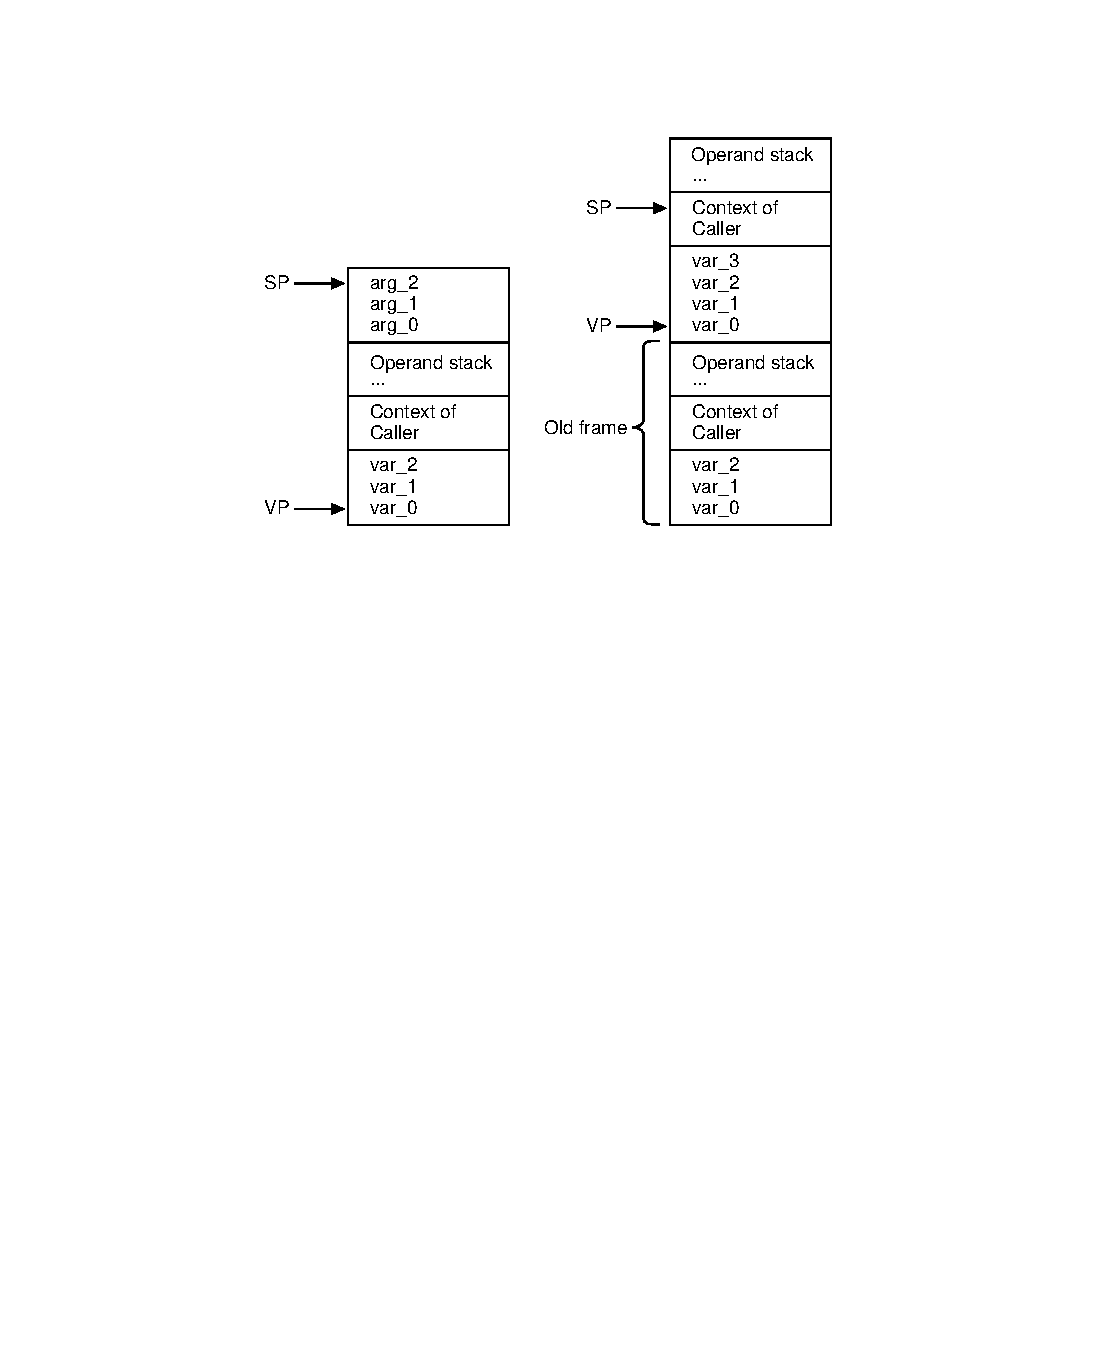
\includegraphics[scale=\picscale]{stack/stack_invocation}
    \caption{Stack change on method invocation}
    \label{fig_stack_invoke}
\end{figure}

\subsection{Access Patterns on the Java Stack}
\label{subsec:access}

The pipelined architecture of a Java processor executes basic
instructions in a single cycle. A stack that contains the operand
stack \emph{and} the local variables results in the following access
patterns:
%
\begin{description}
\item[Stack Operation:] Read of the two top elements, operate on them and
push back the result on the top of the stack. The pipeline stages
for this operation are:\newline
\texttt{
    value1 $\leftarrow $ stack[sp], value2 $\leftarrow $ stack[sp-1]\newline
    result $\leftarrow $ value1 op value2, sp $\leftarrow $ sp-1\newline
    stack[sp] $\leftarrow $ result
}

\item[Variable Load:] Read a data element deeper down in the
    stack, relative to a variable base address pointer (VP), and
    push this data on the top of the stack. This operation needs
    two pipeline stages:\newline \texttt{ value $\leftarrow $
    stack[vp+offset], sp $\leftarrow $ sp+1\newline stack[sp]
    $\leftarrow $ value
}

\item[Variable Store:] Pop the top element of the stack and write it in
the variable relative to the variable base address:\newline
\texttt{
    value $\leftarrow $ stack[sp]\newline
    stack[vp+offset] $\leftarrow $ value, sp $\leftarrow $ sp-1
}
\end{description}
%
For pipelined execution of these operations, a three-port memory or
register file (two read ports and one write port) is necessary.

\subsection{Common Realizations of a Stack Cache}

As the stack is a heavily accessed memory region, the stack -- or
part of it -- has to be placed in the upper level of the memory
hierarchy. This part of the stack is referred to as a \emph{stack
cache}. As described in \cite{Hennessy02}, a typical memory hierarchy
contains the following elements, with increasing access time and
size:
%
\begin{itemize}
\item CPU register
\item On-chip cache memory
\item Off-chip cache memory
\item Main memory
\item Magnetic disk for virtual memory
\end{itemize}
%
For a stack cache, a register file is the solution with the shortest access
time. However, in order to store more than a few elements in the cache, an
on-chip memory realization can provide a larger cache. Both variants have
been used and are described below.

\subsubsection{The Register File as a Stack Cache}

An example of a Java processor that uses a register file is Sun's
picoJava \cite{pjMicroArch}. It contains 64 registers, organized as a
circular buffer. To compensate for this \emph{small} stack cache, an
automatic spill and fill circuit needs another read/write port to the
register file. aJile's JEMCore \cite{880720} is a direct-execution
Java processor core that contains 24 registers. Only six of them are
used to cache the top elements of the stack. With this small register
count, local variables are not part of the cache. Ignite
\cite{IGNITE} (formerly known as PSC1000) is a stack processor,
originally designed as a Forth processor and now promoted as a Java
processor, and has an operand stack that contains 18 registers with
automatic spill and fill.

A basic pipeline for a stack processor with a register file contains the
following stages:
%
\begin{enumerate}
\item IF -- instruction fetch
\item ID -- instruction decode
\item EX -- read register file and execute
\item WB -- write result back to register file
\end{enumerate}
%
With this pipeline structure, a single data-forwarding path between
WB and EX is necessary. The ALU with the register file (with a size
of 16, a common size for RISC processors) and the bypass unit are
shown in Figure~\ref{fig_stack_cache_reg}. In
Table~\ref{tab_resource_reg_cache} the hardware resources of this
type of stack cache are approximated, using the values given in
Table~\ref{tab_simp_gate_count} (a MUX not found in this table is
assumed to use combinations of the basic types; e.g.\ two 8:1 and
one 2:1 for a 16:1). An experimental evaluation of this architecture
in an FPGA is described in Section~\ref{subsec:resource}.

\begin{table}[hbtp]
    \centering
    \begin{tabular}{lc}
        \toprule
        Basic function & Gate count \\
        \midrule
        D-Flip-Flop&5 \\
        2:1 MUX&3 \\
        4:1 MUX&5 \\
        8:1 MUX&9 \\
        SRAM Bit&1.5 \\
        \bottomrule
    \end{tabular}
    \caption{Simplified gate count for basic functions}
    \label{tab_simp_gate_count}
\end{table}

\begin{figure*}
    \centering
    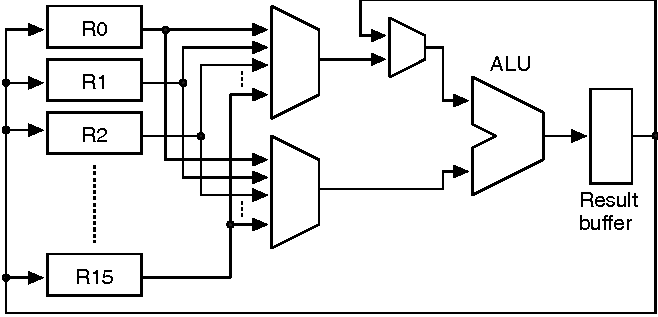
\includegraphics[scale=\picscale]{stack/stack_cache_reg}
    \caption{A stack cache with registers}
    \label{fig_stack_cache_reg}

    \vspace{\floatsep}    % zusaetzlicher Abstand zwischen zwei `floats'

    \begin{tabular}{lld{1}}
        \toprule
        Function block& Basic function& \cc{Gate count} \\
        \midrule
        Register File& 512 D-Flip-Flops& 2,560 \\
        Read MUX& 2x32 16:1 MUX&1,344 \\
        Forward MUX& 32 2:1 MUX&96 \\
        ALU buffer& 32 D-Flip-Flops&160 \\
        \midrule
        \textbf{Total}& &4,160 \\
        \bottomrule
    \end{tabular}
    \captionof{table}{Estimated gate count for a register stack cache}
    \label{tab_resource_reg_cache}
\end{figure*}

\subsubsection{On-chip Memory as a Stack Cache}

Using SRAM on the chip provides a \emph{large} stack cache (e.g.\
128 entries). However, as we have seen in
Section~\ref{subsec:access}, a three-port memory is necessary. An
additional pipeline stage performs the cache memory read:
%
\begin{enumerate}
\item IF -- instruction fetch
\item ID -- instruction decode
\item RD -- memory read
\item EX -- execute
\item WB -- write result back to memory
\end{enumerate}
%
With this pipeline structure, two data forwarding paths are
necessary. The resulting architecture is shown in
Figure~\ref{fig_stack_cache_ram} and a gate count estimate is
provided in Table~\ref{tab_resource_sram_cache}. This version needs
70{\%} more resources than the first one, but provides an eight
times larger stack cache.

Example designs that use this kind of stack cache are (i) Komodo
\cite{Zulauf00}, a Java processor intended as a basis for research
on multithreaded real-time scheduling, and (ii) FemtoJava
\cite{Femto01}, a research project to build an application specific
Java processor.

A three-port memory is an expensive option for an ASIC and unusual
in an FPGA. It can be emulated in an FPGA by two memories with a
single read and write port. The write data is written in both memory
blocks and each memory block provides a different read port.
However, this solution also doubles the amount of memory.

Both designs (Komodo and FemtoJava) avoid the memory doubling by
serializing the two reads. This serialization results in a minimum of
two clock cycles execution time for basic instructions or halves the
clock frequency of the whole pipeline.

\begin{figure*}
    \centering
    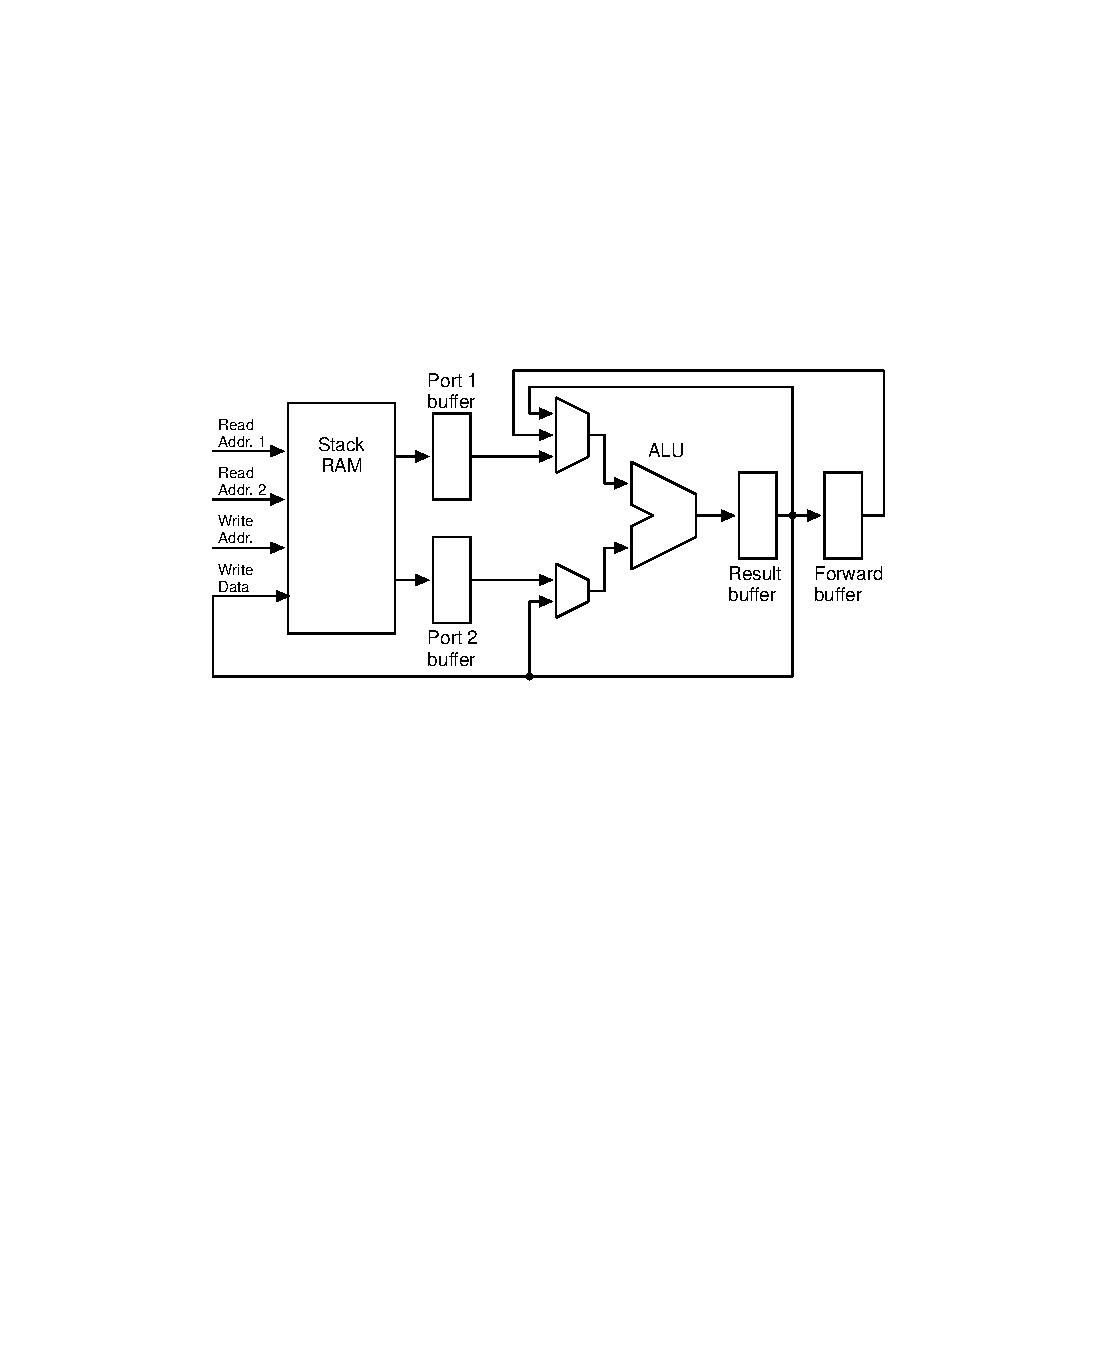
\includegraphics[scale=\picscale]{stack/stack_cache_ram}
    \caption{A stack cache with on-chip RAM}
    \label{fig_stack_cache_ram}

    \vspace{\floatsep}    % zusaetzlicher Abstand zwischen zwei `floats'

    \begin{tabular}{lld{1}}
        \toprule
        Function block& Basic function& \cc{Gate count} \\
        \midrule
        Stack RAM& e.g.\ 128x32 Bits& 6,144 \\
        Port buffer& 2x32 D-Flip-Flops& 320 \\
        Forward MUX& 32x 2:1 MUX, 3:1 MUX& 288 \\
        ALU buffer& 2x32 D-Flip-Flops& 320 \\
        \midrule
        \textbf{Total}& & 7,072 \\
        \bottomrule
    \end{tabular}
    \captionof{table}{Estimated gate count for a stack cache with RAM}
    \label{tab_resource_sram_cache}
\end{figure*}

\subsection{A Two-Level Stack Cache}

In this section, we will discuss access patterns of the JVM and
their implication on the functional units of the pipeline. A faster
and smaller architecture is proposed for the stack cache of a Java
processor.

\subsubsection{JVM Stack Access Revised}

If we analyze the JVM's access patterns to the stack in more detail,
we can see that a two-port read is only performed with the two top
elements of the stack. All other operations with elements deeper in
the stack, local variables load and store, only need one read port.
If we only implement the two top elements of the stack in registers,
we can use a standard on-chip RAM with one read and one write port.

We will show that all operations can be performed with this
configuration. Let $A$ be the top-of-stack, $B$ the element below
top-of-stack. The memory that serves as the second level cache is
represented by the array $sm$. Two indices in this array are used:
$p$ points to the logical third element of the stack and changes as
the stack grows or shrinks, $v$ points to the base of the local
variables area in the stack and $n$ is the address offset of a
variable. $op$ is a two operand stack operation with a single result
(i.e.\ a typical ALU operation).


\begin{description}
\begin{samepage}
\item[Case 1:]
ALU operation \newline \textit{A $\leftarrow $ A op B
\newline B $\leftarrow $ sm[p] \newline p $\leftarrow $ p -- 1
\newline }The two operands are provided by the two top level
registers. A single read access from $sm$ is necessary to fill $B$
with a new value.
\end{samepage}
%
\begin{samepage}
\item[Case 2:]
    Variable load (\textit{Push}) \newline
    \textit{
    sm[p+1]$\leftarrow $ B \newline
    B $\leftarrow $ A \newline
    A$\leftarrow $ sm[v+n] \newline
    p $\leftarrow $ p + 1 \newline
    }
    One read access from \textit{sm} is necessary for the variable read. The
former TOS value moves down to $B$ and the data previously in $B$ is
written to \textit{sm}.
\end{samepage}
%
\begin{samepage}
\item[Case 3:]
    Variable store (\textit{Pop}) \newline
    \textit{sm[v+n] $\leftarrow $ A \newline
    A $\leftarrow $ B \newline
    B $\leftarrow $ sm[p] \newline
    p $\leftarrow $ p - 1 \newline }
    The TOS value is written to \textit{sm}. $A$ is filled with $B$ and $B$ is filled in an
identical manner to Case 1, needing a single read access from
\textit{sm}.
\end{samepage}
\end{description}
%
We can see that all three basic operations can be performed with a
stack memory with one read and one write port. Assuming a memory is
used that can handle concurrent read and write access, there is no
structural access conflict between $A$, $B$ and \textit{sm}. That
means that all operations can be performed concurrently in a single
cycle.

As we can see in Figure~\ref{fig_stack_invoke} the operand stack and
the local variables area are distinct regions of the stack. A
concurrent read from and write to the stack is only performed on a
variable load or store. When the read is from the local variables
area the write goes to the operand area; a read from the operand
area is concurrent with a write to the local variables area.
Therefore there is no concurrent read and write to the same location
in \textit{sm}. There is no constraint on the read-during-write
behavior of the memory (old data, undefined or new data), which
simplifies the memory design. In a design where read and write-back
are located in different pipeline stages, as in the architectures
described above, either the memory must provide the new data on a
read-during-write, or external forward logic is necessary.

From the three cases described, we can derive the memory addresses
for the read and write port of the memory, as shown in
Table~\ref{tab_stack_address}.

\begin{table}[htbp]
    \centering
    \begin{tabular}{cc}
        \toprule
        Read address&Write address \\
        \midrule p&p+1 \\
        v+n&v+n \\
        \bottomrule
    \end{tabular}
    \caption{Stack memory addresses}
    \label{tab_stack_address}
\end{table}

\subsubsection{The Datapath}

The architecture of the two-level stack cache can be seen in
Figure~\ref{fig_stack_cache_jop}. Register $A$ represents the
top-of-stack and register $B$ the data below the top-of-stack. ALU
operations are performed with these two registers and the result is
placed in $A$. During such an ALU operation, $B$ is filled with new
data from the stack RAM. A new value from the local variable area is
loaded directly from the stack RAM into $A$. The data previously in
$A$ is moved to $B$ and the data from $B$ is spilled to the stack
RAM. $A$ is stored in the stack RAM on a store instruction to the
local variable. The data from $B$ is moved to $A$ and $B$ is filled
with a new value from the stack RAM.
%All these operations are performed concurrently in one cycle.

With this architecture, the pipeline can be reduced to three stages:
%
\begin{enumerate}
\item IF -- instruction fetch
\item ID -- instruction decode
\item EX -- execute, load or store
\end{enumerate}
%
The estimated resource usage of this two-level stack cache
architecture is given in Table~\ref{tab_resource_jop_cache}. It can
be seen that this architecture is roughly as complex as the solution
given above (about 5{\%} less gates). However, the reduced
complexity with the two-port RAM instead of a three-port RAM is not
included in the table. The critical path through the ALU contains
only one 2:1 MUX to register $A$ in this solution, rather than one
3:1 MUX in one ALU path and one 2:1 MUX in the other ALU path. As no
data forwarding logic is necessary, the decoding logic is also
simpler.

\begin{figure*}
    \centering
    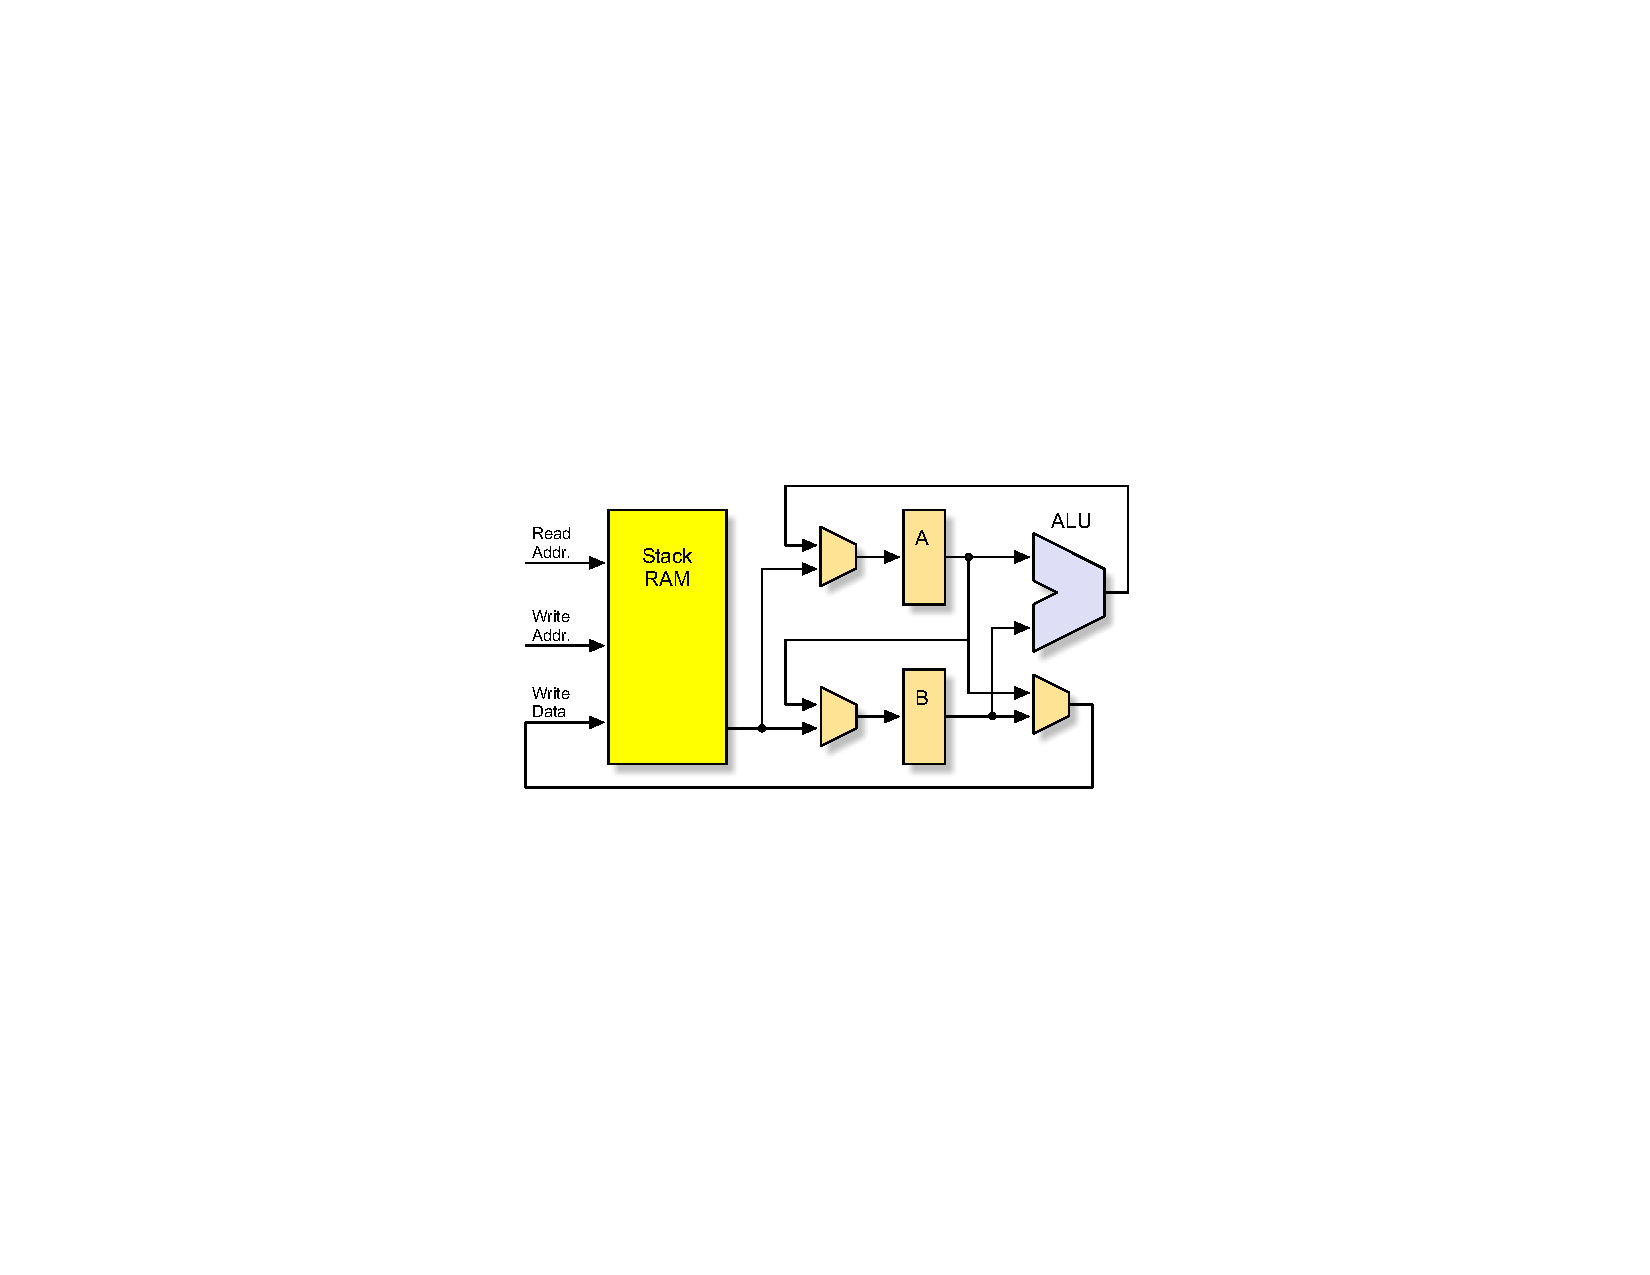
\includegraphics[scale=\picscale]{stack/stack_cache_jop}
    \caption{Two-level stack cache}
    \label{fig_stack_cache_jop}

    \vspace{\floatsep}    % zusaetzlicher Abstand zwischen zwei `floats'

    \begin{tabular}{lld{1}}
        \toprule
        Function block& Basic function& \cc{Gate count} \\
        \midrule
        Stack RAM& e.\ g.\ 128x32 Bits&6,144 \\
        TOS, TOS-1 buffer& 2x32 D-Flip-Flops&320 \\
        Three MUX& 3x32 2:1 MUX&288 \\
        \midrule
        \textbf{Total}& &6,752 \\
        \bottomrule
    \end{tabular}
    \captionof{table}{Estimated gate count for a two-level stack cache}
    \label{tab_resource_jop_cache}
\end{figure*}

\subsubsection{Data Forwarding -- A Non-Issue}

Data dependencies in the instruction stream result in the so-called
\emph{data hazards} \cite{Hennessy02} in the pipeline. Data
forwarding is a technique that moves data from a later pipeline
stage back to an earlier one to solve this problem. The term
\emph{forward} is correct in the temporal domain as data is
transferred to an instruction in the future. However, it is
misleading in the structural domain as the forward direction is
towards the \emph{last} pipeline stage for an instruction.

As the probability of data dependency is very high in a stack-based
architecture, one would expect several data forwarding paths to be
necessary. However, in the two-level architecture proposed, with its
resulting three-stage pipeline, no data hazards will occur and no
data forwarding is therefore necessary. This simplifies the decoding
stage and reduces the number of multiplexers in the execution path.
We will show that none of the three data hazard types
\cite{Hennessy02} is an issue in this architecture. With instructions
$i$ and $j$, where $i$ is issued before $j$, the data hazard types
are:

\paragraph{Read after write:} $j$ reads a source before $i$ writes it. This
is the most common type of hazard and, in the architectures
described above, is solved by using the ALU buffers and the
forwarding multiplexer in the ALU datapath. On a stack architecture,
write takes three forms:
%
\begin{itemize}
    \item Implicit write of TOS during an ALU operation
    \item Write to the TOS during a load instruction
    \item Write to an arbitrary entry of the stack with a store instruction
\end{itemize}
%
A read also occurs in three different forms:
\begin{itemize}
    \item Read two top values from the stack for an ALU operation
    \item Read TOS for a store instruction
    \item Read an arbitrary entry of the stack with the load instruction
\end{itemize}
%
With the two top elements of the stack as discrete registers, these
values are read, operated on and written back in the same cycle. No
read that depends on TOS or TOS-1 suffers from a data hazard. Read
and write access to a local variable is also performed in the same
pipeline stage. Thus, the read after write order is not affected.
However, there is also an additional hidden read and write: the fill
and spill of register B:



%
\begin{itemize}
\item \textit{B fill:}
$B$ is written during an ALU operation and on a variable store.
During an ALU operation, the operands are the values from $A$ and
the old value from $B$. The new value for $B$ is read from the stack
memory and does not depend on the new value of $A$. During a
variable store operation, $A$ is written to the stack memory and
does not depend on $B$. The new value for $B$ is also read from the
stack memory and it is not obvious that this value does not depend
on the written value. However, the variable area and the operand
stack are distinct areas in the stack (this changes only on method
invocation and return), guaranteeing that concurrent read/write
access does not produce a data hazard.

\item \textit{B spill:}
$B$ is read on a load operation. The new value of $B$ is the old
value of $A$ and does not therefore depend on the stack memory read.
$B$ is written to the stack. For the read value from the stack
memory that goes to $A$, the argument concerning the distinct stack
areas in the case of \textit{B fill} described above still applies.
\end{itemize}
%
\paragraph{Write after read:} $j$ writes a destination before it is read by
$i$. This cannot take place as all reads and writes are performed in
the same pipeline stage keeping the instruction order.

\paragraph{Write after write:} $j$ writes an operand before it is written by
$i$. This hazard is not present in this architecture as all writes
are performed in the same pipeline stage.



\subsection{Resource Usage Compared}
\label{subsec:resource}

The three architectures described above are implemented in Altera's
EP1C6Q240C6 \cite{AltCyc} FPGA. The three-port memory for the second
solution is emulated with two embedded memory blocks. The ALU for
this comparison is kept simple with the following functions: NOP,
ADD, SUB, POP, AND, OR, XOR and load external data. The load of
external data is necessary in order to prevent the synthesizer from
optimizing away the whole design. A real implementation of an ALU
for a Java processor, as described in Section~\ref{sec:pipeline}, is
a little bit more complex with a barrel shifter and additional load
paths. In order to gain the maximum operating frequency for the
design, the testbed for this architecture contains registers for the
external data, the RAM address buses, and the control and select
signals. Table~\ref{tab_stack_resources} shows the resource usage
and maximum operation frequency of the three different
architectures.

\begin{table*}
    \centering
    \begin{tabular}{lccccccc}
        \toprule
        Design& \multicolumn{2}{c}{Total}&
        \multicolumn{2}{c}{Cache}&
        Memory& fmax & Size\\
         & LCs& Reg.& LCs&
        Reg.& (bit)& (MHz) & (word)\\
        \midrule
%        ALU only& 194& 0& -& -& -&- &-\\
        Testbed w.\ ALU& 261& 166& -& -& -&237 & - \\
        16 register cache& 968& 657& 707& 491& 0&110 & 16 \\
%        16 Register cache& 297& 140& 36& -26& 1024&113 & 16 \\
        SRAM cache& 372& 185& 111& 19& 8,192&153 & 128\\
        Two-level cache& 373& 184& 112& 18& 4,096& 213 & 130\\
        \bottomrule
    \end{tabular}
    \caption{Resource and performance compared}
    \label{tab_stack_resources}
\end{table*}


LC stands for `Logic Cell' and is the basic element in an FPGA: a
4-bit lookup table with a register. The LC count in the table
includes the register count. The ALU alone without any stack cache
needs 194 LCs. In the first line, the testbed is combined with the
ALU without any stack caching, as a reference design. With this
configuration, we can obtain the maximum possible speed of the
registered ALU in this FPGA technology, in this case an operating
frequency of 237~MHz or a 4.2~ns delay. This value is an upper bound
of the system frequency. Every pipelined architecture needs one or
more multiplexer in the ALU path, either for data forwarding or for
operand selection, resulting in a longer delay. The fourth and fifth
columns represent the resource usage of the cache logic without the
testbed and ALU. The last column shows the effective cache size in
data words.

The version with the 16 registers was synthesized with two different
synthesizer settings. In the first setting, the register file is
implemented with discrete registers while, with a different setting,
the register file is automatically implemented in two 32-bits
embedded RAM blocks. Two different RAM blocks are necessary to
provide two read ports and one write port. In both versions, the
delay time to read the register file (delay through the 16:1 MUX of
4.9~ns or RAM access time of 4.6~ns) is in the same order as the
delay time through the ALU, resulting in a system frequency of half
the theoretical frequency of that with the ALU alone. As the
structure of the version with the embedded RAM block is very similar
with the SRAM cache, only the version with the discrete registers is
shown in Table~\ref{tab_stack_resources}.

The stack cache with a RAM and registers on the RAM output (the
additional pipeline stage) performs better than the first solution.
However, the 3:1 MUX in the critical path still adds 2.3~ns to the
delay time. Compared with the proposed solution (in the last line),
we see that double the amount of RAM is needed for the two read
ports.

The two-level stack cache solution performs at 213~MHz, i.e.\ almost
the theoretical system frequency (in practice, about 10{\%} slower).
Only a 2:1 MUX is added to the critical path. The single read port
memory needs half the number of memory bits of the other two
solutions.

\subsection{Summary}

In this section, the stack architecture of the JVM was analyzed. We
have seen that the JVM is different from the classical stack
architecture. The JVM uses the stack both as an operand stack
\textit{and} as the storage place for local variables. Local
variables are placed in the stack at a \textit{deeper} position. To
load and store these variables, an access path to an arbitrary
position in the stack is necessary. As the stack is the most
frequently accessed memory area in the JVM, caching of this memory
is mandatory for a high-performing Java processor.

A common solution, found in a number of different Java processors,
is to implement this stack cache as a standard three-port register
file with additional support to address this register file in a
stack like manner. The architectures presented above differ in the
realization of the register file: as a discrete register or in
on-chip memory. Implementing the stack cache as discrete registers
is very expensive. A three-port memory is also an expensive option
for an ASIC and unusual in an FPGA. It can be emulated by two
memories with a single read and write port. However, this solution
also doubles the amount of memory.

Detailed analysis of the access patterns to the stack showed that
only the two top elements of the stack are accessed in a single
cycle. Given this fact, the proposed architecture uses registers to
cache only the two top elements of the stack. The next level of the
stack cache is provided by a simple on-chip memory. The memory
automatically spills and fills the second register. Implementing the
two top elements of the stack as fixed registers, instead of
elements that are indexed by a stack pointer, also greatly
simplifies the overall pipeline.

The proposed stack architecture has the following advantages: (i)
Simpler cache memory results in having half the memory usage of the
other solutions in an FPGA. (ii) Minimal impact on the raw speed of
the ALU. Operates at almost the theoretical maximum system frequency
of the ALU. (iii) Single read, execute and write-back pipeline stage
results in an overall 3-stage pipeline processor design. (iv) No
data forwarding is necessary, which simplifies instruction decode
logic and reduces the multiplexer count in the critical path.


\clearpage
    
\section{HW/SW Codesign}
\label{sec:hwsw:co}

Using a hardware description language and loading the design in an
FPGA the former strict border between hardware and software gets
blurred. Is configuring an FPGA not more like loading a program for
execution?

This looser distinction makes it possible to move functions easily
between hardware and software resulting in a highly configurable
design. If speed is an issue, more functions are realized in
hardware. If cost is the primary concern these functions are moved
to software and a smaller FPGA can be used. Let us examine these
possibilities on a relatively expensive function:
\emph{multiplication}.

Bytecode \code{imul} performs a 32 bit signed multiplication with a
32 bit result. There are no exceptions on overflow. Since 32 bit
single cycle multiplications are far beyond the possibilities of
current, mainstream FPGAs the first solution is a sequential
multiplier.

\paragraph{Sequential Booth Multiplier in VHDL}

\begin{lstlisting}[float, caption={Booth multiplier in VHDL},
language=VHDL, label=lst:arch:hwsw:vhdl]
    process(clk, wr_a, wr_b)

        variable count  : integer range 0 to width;
        variable pa     : signed(64) downto 0);
        variable a_1    : std_logic;
        alias p         : signed(32 downto 0)
                          is pa(64 downto 32);

    begin
        if rising_edge(clk) then
            if wr_a='1' then
                p := (others => '0');
                pa(width-1 downto 0) := signed(din);

            elsif wr_b='1' then
                b <= din;
                a_1 := '0';
                count := width;
            else
                if count > 0 then
                    case std_ulogic_vector'(pa(0), a_1) is
                        when "01" =>
                            p := p + signed(b);
                        when "10" =>
                            p := p - signed(b);
                        when others =>
                            null;
                    end case;
                    a_1 := pa(0);
                    pa := shift_right(pa, 1);
                    count := count - 1;
                end if;
            end if;
        end if;
        dout <= std_logic_vector(pa(31 downto 0));
    end process;
\end{lstlisting}
%
Listing~\ref{lst:arch:hwsw:vhdl} shows the VHDL code of the
multiplier. Two microcode instructions are used to access this
function: \code{stmul} stores the two operands (from TOS and TOS-1)
and starts the sequential multiplier. After 33 cycles, the result is
loaded with \code{ldmul}. Listing~\ref{lst:arch:hwsw:micro} shows
the microcode for \code{imul}.

\begin{lstlisting}[float, caption={Microcode to access the Booth multiplier},
label=lst:arch:hwsw:micro]
    imul:
            stmul       // store both operands and start
            pop         // pop second operand

            ldi 5       // 6*5+3 cycles wait
imul_loop:              // wait loop
            dup
            nop
            bnz imul_loop
            ldi -1      // decrement in branch slot
            add

            pop         // remove counter

            ldmul   nxt // load result
\end{lstlisting}

\paragraph{Multiplication in Microcode}

If we run out of resources in the FPGA, we can move the function to
microcode. The implementation of \code{imul} is almost identical to
the Java code in Listing~\ref{lst:arch:hwsw:java} and needs 73
microcode instructions.

\paragraph{Bytecode imul in Java}

Microcode is stored in an embedded memory block of the FPGA. This is
also a resource of the FPGA. We can move the code to external memory
by implementing \code{imul} in Java bytecode. Bytecodes not
implemented in microcode result in a static Java method call from a
special class (\code{com.jopdesign.sys.JVM}). This class has
prototypes for each bytecode ordered by the bytecode value. This
allows us to find the right method by indexing the method table with
the value of the bytecode. Listing~\ref{lst:arch:hwsw:java} shows
the Java method for \code{imul}. The additional overhead for this
implementation is a call and return with cache refills.


\begin{lstlisting}[float, caption={Implementation of bytecode \code{imul} in Java},
label=lst:arch:hwsw:java]
    public static int imul(int a, int b) {

        int c, i;
        boolean neg = false;
        if (a<0) {
            neg = true;
            a = -a;
        }
        if (b<0) {
            neg = !neg;
            b = -b;
        }
        c = 0;
        for (i=0; i<32; ++i) {
            c <<= 1;
            if ((a & 0x80000000)!=0) c += b;
            a <<= 1;
        }
        if (neg) c = -c;
        return c;
    }
\end{lstlisting}

\paragraph{Implementations Compared}

\tablename~\ref{tab_arch_hwsw_compared} lists the resource usage and
execution time for the three implementations. Execution time is
measured with both operands negative, the worst-case execution time
for the software implementations. The implementation in Java is
slower than the microcode implementation as the Java method is
loaded from main memory into the bytecode cache.

\begin{table}
    \centering
    \begin{tabular}{ld{2}d{3}d{0}}
    \toprule
    & \cc{Hardware} & \cc{Microcode} & \cc{Time} \\
    & \cc{[LC]} & \cc{[Byte]} & \cc{[Cycle]} \\
    \midrule
    VHDL & 156 & 10 & 35 \\
    Microcode & 0 & 73 & 750 \\
    Java & 0 & 0 & ~2,300 \\
    \bottomrule
    \end{tabular}
    \caption{Different implementations of \code{imul} compared}
    \label{tab_arch_hwsw_compared}
\end{table}

Only a few lines of code have to be changed to select one of the
three implementations. This principle can also be applied to other
expensive bytecodes: e.g.\ \code{idiv}, \code{ishr}, \code{iushr} and
\code{ishl}. As a result, the resource usage of JOP is highly
configurable and can be selected for each application according to
the needs of the application. Treating VHDL as a software language
allows easy movement of function blocks between hardware and
software.

\clearpage
    
\section{Real-Time Predictability}
\label{sec:rtpredict}

%%% part of that intro is found in the cache section

%\subsection{Time Predictable Architecture}
%
%Worst case execution time (WCET) analysis of real-time programs is
%essential for any schedulability analysis. To provide a tight WCET
%value a good model of the processor is necessary. However, the
%architectural advancement in modern processor designs is dominated
%by the rule: '\emph{Make the common case fast}`. This is the
%opposite to: '\emph{Reduce the worst case}` and complicates WCET
%analysis. JOP was designed to provide an architecture that can be
%exactly modeled. Execution time of bytecodes is known cycle
%accurate. It is possible to analyze the timing on the bytecode level
%without the uncertainties of an interpreting JVM or generated native
%code from ahead-of-time compilers for Java.
%
%
%Common architectural components, such as branch prediction and
%branch target buffers enhance average performance, but have usually
%a very pessimistic WCET. In JOP, branch prediction is avoided. This
%results in pressure on the pipeline length. The processor has a
%minimal pipeline length of four stages resulting in a four cycle
%execution time for a bytecode branch.
%
%The stack is a frequently accessed memory area and therefore
%implemented in on-chip memory and serving as data cache. Data
%exchange between internal stack and main memory is under microcode
%control and therefore WCET analyzable.
%
%Instruction cache is mandatory to bridge the growing gap between CPU
%speed and main memory access time. Standard cache organizations
%improve average execution time, but are hard to predict for worst
%case execution time (WCET) analysis. We tackled this problem from
%the architectural side: An instruction cache organization where
%simpler and more accurate WCET analysis is more important than
%average case performance.
%
%JOP has a novel instruction cache: A \emph{method cache}. A complete
%method is loaded in the cache on invocation and on return. This
%cache fill strategy lumps all cache misses together and is very
%simple to analyze. Cache block replacement depends on the call tree
%instead of instruction addresses and is therefore WCET analyzable.
%
%
%Comparing this cache organization quantitative with a benchmark
%derived from a real-time application we have seen that the proposed
%\emph{method cache} performs similar or even better to a traditional
%direct mapped cache with respect to the bytes that have to be filled
%an a cache miss. The number of memory transactions, which result in a
%high miss penalty on memories with high latency, are lower with the
%proposed cache solution than in a traditional cache.
%
%




General-purpose processors are optimized for average throughput and
non real-time operating systems are responsible for fair and
efficient scheduling of resources. Real-time systems need a
processor with low and known WCET of instructions. Real-time
operating systems have properties, such as fast interrupt response,
rapid context switch, short blocking times and a scheduler that
implements a simple, in most cases strict priority driven,
scheduling algorithm. This section describes design decisions for
JOP to support such real-time systems.

\subsection{Interrupts}

Interrupts are usually associated with low-level programming of
device drivers. The priorities of interrupts and their handler
functions are above task priorities and yield to an immediate
context switch. In this form, interrupts cannot be integrated in a
schedule with \emph{normal} tasks. The execution time of the
interrupt handler has to be integrated in the schedulability
analysis as additional blocking time. A better solution is to handle
interrupts, which represent external events, as schedulable objects
with priority levels in the range of real-time tasks, as suggested
in the RTSJ.

\paragraph{The Timer Interrupt}

The timer or clock interrupt has a different semantic than other
interrupts. The main purpose of the timer interrupt is
representation of time and release of periodic or time triggered
tasks. One common implementation is a clock tick. The interrupt
occurs at a regular interval (e.g.\ 10 ms) and a decision has to be
taken whether a task has to be released. This approach is simple to
implement, but there are two major drawbacks: The resolution of
timed events is bound by the resolution of the clock tick and clock
ticks without a task switch are a waste of execution time.

A better approach, used in JOP, is to generate timer interrupts at
the release times of the tasks. The scheduler is now responsible for
reprogramming the timer after each occurrence of a timer interrupt.
The list of sleeping threads has to be searched to find the nearest
release time in the future of a higher priority thread than the one
that will be released now. This time is used for the next timer
interrupt.

\paragraph{External Events}

Hardware interrupts, other than the timer interrupt, are represented
as asynchronous events with an associated thread. This means that
the event is a \emph{normal} schedulable object under the control of
the scheduler. With a minimum interarrival time, enforced by
hardware, these events can be incorporated into the priority
assignment and schedulability analysis in the same way as periodic
tasks.

\paragraph{Software Interrupts}

The common software generated interrupts, such as illegal memory
access or divide by zero, are represented by Java runtime exceptions
and need no special handler. They can be detected with a try-catch
block.

Asynchronous notification from the program is supported, in the same
way as an external event, as a schedulable object with an associated
thread. The event is triggered through the call of \code{fire()}.
The thread with the handler is placed in the runnable state and
scheduled according to priority.

\paragraph{Hardware Failures}

Serious hardware failures, such as illegal opcode or parity error
from the memory systems, lead to a shutdown of the system. However,
a \emph{last try} to call a handler that changes the state of the
system to a safe state and inform an upper level system, can improve
the integrity of the overall system.

\subsection{Task Switch}

An important issue in real-time systems is the time for a task
switch. A task switch consists of two actions:
\begin{itemize}
    \item \emph{Scheduling} is the selection of the task order and timing
    \item \emph{Dispatching} is the term for the context switch between tasks
\end{itemize}

\paragraph{Scheduling}

Most real-time systems use a fixed-priority preemptive scheduler.
Tasks with the same priority are usually scheduled in a FIFO order.
Two common ways to assign priorities are rate monotonic or, in a
more general form, deadline monotonic assignment. When two tasks get
the same priority, we can choose one of them and assign a higher
priority to that task and the task set is still schedulable. We get
a strictly monotonic priority order and do not have to deal with
FIFO order. This eliminates queues for each priority level and
results in a single, priority ordered task list.

Strictly fixed priority schedulers suffer from a problem called
\emph{priority inversion} \cite{626613}. The problem where a low
priority task blocks a high priority task on a shared resource is
solved by raising the priority of the low priority task. Two
standard priority inversion avoidance protocols are common:
%
\begin{description}
    \item[Priority Inheritance Protocol:] A lock assigns the priority
of the highest-priority waiting task to the task holding the lock
until that task releases the resource.

    \item[Priority Ceiling Emulation Protocol:] A lock gets a priority
assigned above the priority of the highest-priority task that will
ever acquire the lock. Every task will be immediately assigned the
priority of that lock when acquiring it.
\end{description}
%
The priority inheritance protocol is more complex to implement and
the time when the priority of a task is raised is not so obvious. It
is not raised because the task does anything, but because another
task reaches some point in its execution path.

Using priority ceiling emulation with unique priorities, different
from task priorities, the priority order is still strictly
monotonic. The priority ordered task list is expanded with slots for
each lock. If a task acquires a lock, it is placed in the
corresponding slot. With this extension to the task list, scheduling
is still simple and can be efficiently implemented.

\paragraph{Dispatching}


The time for a context switch depends on the size of the state of
the tasks. For a stack machine it is not so obvious what belongs to
the state of a task. If the stack resides in main memory, only a few
registers (e.g. program counter and stack pointer) need to be saved
and restored. However, the stack is a frequently accessed memory
region of the JVM. The stack can be seen as a data cache and should
be placed near the execution unit (in this case, \emph{near} means
on the chip and not in external memory). However, on-chip memory is
usually too small to hold the stack content for all tasks. This
means that the stack is part of the execution context and has to be
saved and restored on a context switch.

In JOP, the stack is placed in local (on-chip) FPGA memory with
single cycle access time. With this configuration, the next question
is how much of the stack to place there. Either the complete stack
of a thread or only the stack frame of the current method can reside
locally. If the complete stack of a thread is stored in local
memory, the invocation of methods and returns are fast, but the
context is large. For fast context switches, it is preferable to
have only a short stack in local memory. This results in less data
being transferred to and from main memory, but more memory transfers
on method invocation and return. The local stack can be further
divided into small pieces, each holding only one stack frame of one
thread. During the context switch, only the stack pointer needs to
be saved and restored. The outcome of this is a very fast context
switch, although the size of the local memory limits the maximum
number of threads.

Since JOP is a soft-core processor, these different solutions can be
configured for different application requirements. It is even
possible to mix of these policies: some stack slots can be assigned
to \emph{important} threads, while the remaining threads share one
slot. This stack slot only needs to be exchanged with the main
memory when switching \emph{to} a less \emph{important} thread.

\subsection{Architectural Design Decisions}

In hard real-time systems, meeting temporal requirements is of the
same importance as functional correctness. This results in different
architectural constraints than in a design for a non real-time
system. A low upper bound of the execution time is of premium
importance. Good average execution time is useless for a pure hard
real-time system.

Common architectural components, found in general purpose processors
to enhance average performance, are usually problematic for the WCET
analysis. A pragmatic approach to this problem is to ignore these
features for the analysis. With a processor designed for real-time
applications, these features have to be substituted by predictable
architecture enhancements.

\paragraph{Branch Prediction}

As the pipelines of current general-purpose processors get longer to
support higher clock rates the penalty of branches get too high.
This is compensated by branch prediction logic with branch target
buffers. However, the upper bound of the branch execution time is
the same as without this feature. In JOP, branch prediction is
avoided. This results in pressure on the pipeline length. The core
processor has a pipeline length of as little as three stages
resulting in a branch execution time of three cycles in microcode.
The two slots in the branch delay can be filled with instructions or
\emph{nop}. With the additional bytecode fetch and translation
stage, the overall pipeline is four stages and results in a four
cycle execution time for a bytecode branch.

\paragraph{Caches and Instruction Prefetch}

To reduce the growing gap between the clock frequency of the
processor and memory access times multi-level cache architectures
are commonly used. Since even a single level cache is problematic
for WCET analysis, more levels in the memory architecture are almost
not analyzable. The additional levels also increase the latency of
memory access on a cache miss.

In a stack machine, the stack is a frequently accessed memory area.
This makes the stack an ideal candidate to be placed near the
execution unit in the memory hierarchy. In JOP the stack is
implemented as internal memory with the two top elements as explicit
registers. This single cycle memory can be seen as a data cache.
However, unlike in picoJava, this limited memory is not
automatically spilled and filled. Automatically spill and fill
introduces unpredictable access to the main memory. Data exchange
between internal stack and main memory is under program control and
can be done on method invocation/return or on a thread switch.

The next most accessed memory area is the code area. A simple
prefetch queue, as it is found in older processors, could increase
instruction throughput after executing a multi-cycle bytecode. For a
stream of single cycle bytecodes, prefetching is useless and the
frequent occurrence of branches and method invocations, about
12--23\% (see Section~\ref{sec:bench:jvm}) in typical Java programs,
reduces the performance gain. The prefetch queue also results in
(probably unbounded) execution time dependencies over a stream of
instructions, which complicates timing analysis.

JOP has a method cache with a novel replace policy. Since typical
methods in Java programs are short and there are only relative
branches in a method, a complete method is loaded in the cache on
invocation and on return. This cache fill strategy lumps all cache
misses together and is very simple to analyze. It also simplifies
the hardware of the cache since no tag memory or address translation
is necessary. The \emph{romizer} tool JavaCodeCompact checks the
maximum allowed method size. Section~\ref{sec:cache} describes the
proposed cache solution in detail. Memory areas for the heap and
class description with the constant pool are not cached in JOP.

\paragraph{Superscalar Processors}

A superscalar processor consists of several execution units and
tries to extract instruction level parallelism (ILP) with out of
order execution. Again, this is a nightmare for timing analysis. The
code for a stack machine has less implicit parallelism than a
register machine.

One form of enhancement, usually implemented in stack machines, is
instruction folding. The instruction stream is scanned to find
frequent patterns like load-load-add-store and substitutes these
four instructions with one, RISC-like, operation. There are two
issues with instruction folding in JOP: The combined instruction
needs two read and one write access to the stack in a single cycle.
This would result in doubling of the internal memory usage in the
FPGA. It also needs, at minimum, four bytes read access to the
method cache. To overcome word boundaries, prefetching has to be
introduced after the method cache. This results in an additional
pipeline stage, time dependency of instructions with a more complex
analysis and more hardware resources for the multiplexers.

Programs for embedded and real-time systems are usually
multi-threaded. In future work, it will be investigated if the
additional hardware resources needed for ILP can be better used with
additional processor cores utilizing this implicit thread-level
parallelism.

\paragraph{Time-Predictable Instructions}

A good model of a processor with accurate timing information is
essential for a tight WCET analysis. The architecture of JOP and the
microcode are designed with this in mind. Execution time of
bytecodes is known cycle accurately (see Section~\ref{sec:wcet} and
Appendix~\ref{appx:bytecode}). It is possible to analyze the WCET on
the bytecode level \cite{R:Bernat:2000a} without the uncertainties
of an interpreting JVM \cite{R:Bate:2000a} or generated native code
from ahead-of-time compilers for Java.

\subsection{Summary}

In this section, we argued that, while common techniques in
processor architectures increase average throughput, they are not
feasible for real-time systems. The influence of these architectural
enhancements is at best hardly WCET-analyzable.

The proposed alternatives influence the processor architecture, as
described in earlier sections, as well as the software architecture
that will be described in Section~\ref{sec:rtprof}.

However, the most important architectural enhancement for pipelined
machines is caching, which is necessary even in embedded systems. We
have shown in Section~\ref{sec:stack} how a time-predictable data
cache for a stack machine can be implemented. In the following
section, we will propose a time-predictable cache for instructions.


\clearpage
    \section{A Time-Predictable Instruction Cache}
    \label{sec:cache}
    \label{sec:cache}


Worst-case execution time (WCET) analysis \cite{pusch:maxt:jnl} of
real-time programs is essential for any schedulability analysis. To
provide a low WCET value, a good processor model is necessary.
However, caches for the instructions and data is a classic example of
the paradigm \emph{Make the common case fast}, which complicates WCET
analysis. Avoiding or ignoring this feature in real-time systems, due
to its unpredictable behavior, results in a very pessimistic WCET
value. Plenty of effort has gone into research into integrating the
instruction cache in the timing analysis of tasks \cite{Arnold1994,
Healy1995, 225068} and the influence of the cache on task preemption
\cite{279589, Mataix:1996}. The influence of different cache
architectures on WCET analysis is described in
\cite{Heckmann:IEEE2003}.

We will tackle this problem from the architectural side -- an
instruction cache organization in which simpler and more accurate
WCET analysis is more important than average case performance.

In this section, we will explore the method cache, as it is
implemented in JOP, with a novel replacement policy. In Java bytecode
only relative branches exist, and a method is therefore only left
when a return instruction has been executed.\footnote{An uncaught
exception also results in a method exit.} It has been observed that
methods are typically short (see \cite{jop:thesis}) in Java
applications. These properties are utilized by a cache architecture
that stores complete methods. A complete method is loaded into the
cache on both invocation and return. This cache fill strategy lumps
all cache misses together and is very simple to analyze.

The method cache was first presented in \cite{jop:jtres_cache} and is
now also used by the Java processor SHAP \cite{shap:mcache}.
Furthermore, the idea has been adapted for a processor that executes
compiled C programs \cite{Metzlaff:SPM:2008}.

\subsection{Method Cache}

In this section, we will develop a solution for a time-predictable
instruction cache. Typical Java programs consist of short methods.
There are no branches out of the method and all branches inside are
relative. In the proposed architecture, the full code of a method is
loaded into the cache before execution. The cache is filled on
invocations and returns. This means that all cache fills are lumped
together with a known execution time. The full loaded method and
relative addressing inside a method also result in a simpler cache.
Tag memory and address translation are not necessary.

In the method cache several cache blocks (similar to cache lines) are
used for a method. The main difference from a conventional cache is
that the blocks for a method are all loaded at once and need to be
consecutive.

Choosing the block size is now a major design decision. Smaller
block sizes allow better memory usage, but the search time for a hit
also increases.

With varying block numbers per method, an LRU replacement becomes
impractical. When the method found to be LRU is smaller than the
loaded method, this new method invalidates two cached methods.

For the replacement, we will use a pointer $next$ that indicates the
start of the blocks to be replaced on a cache miss. Two practical
replace policies are:
%
\begin{description}
\item [Next block:]At the very first beginning, $next$ points to the
first block. When a method of length $l$ is loaded into the block
$n$, $next$ is updated to $(n+l)\;mod\;block\;count$.
\item [Stack oriented:]$next$ is updated in the same way as before
on a method load. It is also updated on a method return --
independent of a resulting hit or miss -- to point to the first
block of the leaving method.
\end{description}
%
We will show the operation of these different replacement policies
in an example with three methods: a(), b() and c() of block sizes 2,
2 and 1. The cache consists of 4 blocks and is therefore too small
to hold all the methods during the execution of the code fragment
shown in Listing~\ref{lst:cache:replace}.
%
\begin{samepage}
\begin{lstlisting}[float,caption={Code fragment for the replacement example},
label=lst:cache:replace]
    a() {
        for (;;) {
            b();
            c();
        }
        ...
    }
\end{lstlisting}
\end{samepage}
%
Tables \ref{tab_cache_replace_next} and
\ref{tab_cache_replace_stack} show the cache content during program
execution for both replacement policies. The content of the cache
blocks is shown after the execution of the invoke or return
instruction. An uppercase letter indicates that this block has been
newly loaded. A right arrow depicts the block to be replaced on a
cache miss (the \emph{next} pointer). The last row shows the number
of blocks that are filled during the execution of the program.

\begin{table}
    \centering
\begin{tt}
    \begin{tabular}{lrrrrrrrrrrr}
    \toprule

                &a()    &b()    &ret    &c()    &ret    &b()    &ret    &c()    &ret    &b()    &ret    \\
    \midrule
    \rm{Block 1}&A      &$\to$a &$\to$a &C      &c      &B      &b      &b      &$\to$- &B      &b      \\
    \rm{Block 2}&A      &a      &a      &$\to$- &A      &$\to$a &$\to$a &C      &c      &B      &b      \\
    \rm{Block 3}&$\to$- &B      &b      &b      &A      &a      &a      &$\to$- &A      &$\to$a &$\to$a \\
    \rm{Block 4}&-      &B      &b      &b      &$\to$- &B      &b      &b      &A      &a      &a      \\
    \midrule
    \rm{Fill}      &2   &4      &       &5      &7      &9      &       &11     &13     &15     &       \\
    \bottomrule

    \end{tabular}
\end{tt}
    \caption{Next block replacement policy}
    \label{tab_cache_replace_next}
\end{table}

\begin{table}
    \centering
\begin{tt}
    \begin{tabular}{lrrrrrrrrrrr}
    \toprule

                &a()    &b()    &ret    &c()    &ret    &b()    &ret    &c()    &ret    &b()    &ret    \\
    \midrule
    \rm{Block 1}&A      &$\to$a &a      &a      &a      &$\to$a &a      &a      &a      &$\to$a &a      \\
    \rm{Block 2}&A      &a      &a      &a      &a      &a      &a      &a      &a      &a      &a      \\
    \rm{Block 3}&$\to$- &B      &$\to$b &C      &$\to$c &B      &$\to$b &C      &$\to$c &B      &$\to$b \\
    \rm{Block 4}&-      &B      &b      &$\to$- &-      &B      &b      &$\to$- &-      &B      &b      \\
    \midrule
    \rm{Fill}      &2   &4      &       &5      &       &7      &       &8      &       &10     &       \\
    \bottomrule

    \end{tabular}
\end{tt}
    \caption{Stack oriented replacement policy}
    \label{tab_cache_replace_stack}
\end{table}

In this example, the stack oriented approach needs fewer fills, as
only methods b() and c() are exchanged and method a() stays in the
cache. However, if, for example, method b() is the size of one
block, all methods can be held in the cache using the the \emph{next
block} policy, but b() and c() would be still exchanged using the
\emph{stack} policy. Therefore, the first approach is used in the
proposed cache.


\subsection{WCET Analysis}

\label{sec:cache:wcet}

The proposed instruction cache is designed to simplify WCET
analysis. Due to the fact that all cache misses are only included in
two instructions (\emph{invoke} and \emph{return}), the instruction
cache can be ignored on all other instructions. The time needed to
load a complete method is calculated using the memory properties
(latency and bandwidth) and the length of the method. On an invoke,
the length of the invoked method is used, and on a return, the
method length of the caller is used to calculate the load time.

With a single method cache this calculation can be further
simplified. For every invoke there is a corresponding return. That
means that the time needed for the cache load on return can be
included in the time for the invoke instruction. This is simpler
because both methods, the caller and the callee, are known at the
occurrence of the invoke instruction. The information about which
method was the caller need not be stored for the return instruction
to be analyzed.

With more than one method in the cache, a cache hit detection has to
be performed as part of the WCET analysis. If there are only two
blocks, this is trivial, as (i) a hit on invoke is only possible if
the method is the same as the last invoked (e.g.\ a single method in
a loop) and (ii) a hit on return is only possible when the method is
a leaf in the call tree. In the latter case, it is always a hit.

When the cache contains more blocks (i.e.\ more than two methods can
be cached), a part of the call tree has to be taken into account for
hit detection. The method cache further complicates the analysis, as
the method length also determines the cache content. However, this
analysis is still simpler than a cache modeling of a direct-mapped
instruction cache, as cache block replacement depends on the call
tree instead of instruction addresses.

In traditional caches, data access and instruction cache fill
requests can compete for the main memory bus. For example, a load or
store at the end of the processor pipeline competes with an
instruction fetch that results in a cache miss. One of the two
instructions is stalled for additional cycles by the other
instruction. With a data cache, this situation can be even worse.
The worst-case scenario for the memory stall time for an instruction
fetch or a data load is two miss penalties when both cache reads are
a miss. This unpredictable behavior leads to very pessimistic WCET
bounds.

A \emph{method cache}, with cache fills only on invoke and return,
does not interfere with data access to the main memory. Data in the
main memory is accessed with \emph{getfield} and \emph{putfield},
instructions that never overlap with \emph{invoke} and
\emph{return}. This property removes another uncertainty found in
traditional cache designs.


\subsection{Caches Compared}

In this section, we will compare the different cache architectures
in a quantitative way. Although our primary concern is
predictability, performance remains important. We will therefore
first present the results from a conventional direct-mapped
instruction cache. These measurements will then provide a baseline
for the evaluation of the proposed architecture.

Cache performance varies with different application domains. As the
proposed system is intended for real-time applications, the
benchmark for these tests should reflect this fact. However, there
are no standard benchmarks available for embedded real-time systems.
A real-time application was therefore adapted to create this
benchmark. The application is from one node of a distributed motor
control system \cite{jop:wises03} (see also
Section~\ref{sec:app:kfl}). A simulation of the environment (sensors
and actors) and the communication system (commands from the master
station) forms part of the benchmark for simulating the real-world
workload.

The data for all measurements was captured using a simulation of JOP
and running the application for 500,000 clock cycles. During this
time, the major loop of the application was executed several hundred
times, effectively rendering any misses during the initialization
code irrelevant to the measurements.

\subsubsection{Direct-Mapped Cache}

\tablename~\ref{tab_cache_direct} gives the memory bytes and memory
transactions per instruction byte for a standard direct-mapped
cache. As we can see from the values for a cache size of 4KB, the
kernel of the application is small enough to fit completely into the
4KB cache. The cache performs better (i.e.\ fewer bytes are
transferred) with smaller block sizes. With smaller block sizes, the
chance of unused data being read is reduced and the larger number of
blocks reduces conflict misses. However, reducing the block size
also increases memory transactions (MTIB), which directly relates to
memory latency.


\begin{table}
    \centering
    \begin{tabular}{cd{2.0}cc}
    \toprule

    Cache size & \cc{Block size} & MBIB & MTIB \\

    \midrule

     1 KB &  8 & 0.28 & 0.035 \\
     1 KB & 16 & 0.38 & 0.024 \\
     1 KB & 32 & 0.58 & 0.018 \\
     2 KB &  8 & 0.17 & 0.022 \\
     2 KB & 16 & 0.25 & 0.015 \\
     2 KB & 32 & 0.41 & 0.013 \\
     4 KB &  8 & 0.00 & 0.001 \\
     4 KB & 16 & 0.01 & 0.000 \\
     4 KB & 32 & 0.01 & 0.000 \\

    \bottomrule

    \end{tabular}
    \caption{Direct-mapped cache}
    \label{tab_cache_direct}
\end{table}

Which configuration performs best depends on the relationship between
memory bandwidth and memory latency. Examples of average memory
access times in cycles per instruction byte for different memory
technologies are provided in Table~\ref{tab_cache_direct_mem}. The
third column shows the cache performance for a Static RAM (SRAM) that
is very common in embedded systems. A latency of 1 clock cycle and an
access time of 2 clock cycles per 32-bit word are assumed. For the
synchronous DRAM (SDRAM) in the forth column, a latency of 5 cycles
(3 cycles for the row address and 2 cycles for the CAS latency) is
assumed. The memory delivers one word (4 bytes) per cycle. The Double
Data Rate (DDR) SDRAM in the last column has an enhanced latency of
4.5 cycles and transfers data on both the rising and falling edge of
the clock signal.

%
%       simulate 32-bits (DDR) SDRAM
%
%       SDRAM:  5 cycle latency: 3 cycle row address and 2 cycle CAS latency
%               4 Bytes / cycle (0.25 / Byte)
%
%       DDR:    4.5 cycle latency: 2 cycle row address and 2.5 cycle CAS latency
%               4 Bytes / 0.5 cycle (0.125 / Byte)
%
%       SRAM 15 ns at 100 MHz: 1 cycle latency, 2 cycles / word
%


\begin{table}
    \centering
    \begin{tabular}{cd{2.0}ccc}
    \toprule

    Cache size & \cc{Block size} & SRAM & SDRAM & DDR \\

    \midrule

    1 KB & 8 & \textbf{0.18} & 0.25 & 0.19 \\
    1 KB & 16 & 0.22 & \textbf{0.22} & 0.16 \\
    1 KB & 32 & 0.31 & 0.24 & \textbf{0.15} \\
    2 KB & 8 & \textbf{0.11} & 0.15 & 0.12 \\
    2 KB & 16 & 0.14 & \textbf{0.14} & \textbf{0.10} \\
    2 KB & 32 & 0.22 & 0.17 & 0.11 \\

    \bottomrule

    \end{tabular}
    \caption{Direct-mapped cache, average memory access time}
    \label{tab_cache_direct_mem}
\end{table}

The data in bold give the best block size for different memory
technologies. As expected, memories with a higher latency and
bandwidth perform better with larger block sizes. For small block
sizes, the latency clearly dominates the access time. Although the
SRAM has half the bandwidth of the SDRAM and a quarter of the DDR,
with a block size of 8 bytes, it is faster than the DRAM memories.
In most cases a block size of 16 bytes is the fastest solution and
we will therefore use this configuration for comparison with the
following cache solutions.

\subsubsection{Fixed Block Cache}

Cache performance for single method per block architectures is shown
in Table~\ref{tab_cache_block}. The measurements for a simple 8 byte
prefetch queue are also given, for reference. With prefetching, we
would expect to see an MBIB of about 1. The 37\% overhead results
from the fact that the prefetch queue fetches 4 bytes a time and has
to buffer a minimum of 3 bytes for the instruction fetch stage. On a
branch or return, the queue is flushed and these bytes are lost.

A single block that has to be filled on every invoke and return
requires considerable overheads. More than twice the amount of data
is read from the main memory than is consumed by the processor.
However, the memory transaction count is 16 times lower than with
simple prefetching, which can compensate for the large MBIB for main
memories with high latency.

The solution with two blocks for two methods performs almost twice
as well as the simple one method cache. This is due to the fact
that, for all leaves in the call tree, the caller method can be
found on return. If the block count is doubled again, the number of
misses is reduced by a further 25\%, but the cache size also
doubles. For this measurement, an LRU replacement policy applies for
the two and four block caches.

\begin{table}
    \centering
    \begin{tabular}{lcccc}
    \toprule

    Type & Cache size & MBIB & MTIB \\

    \midrule
        Prefetch & 8 B & 1.37 & 0.342  \\
        Single method & 1 KB & 2.32 & 0.021  \\
        Two blocks & 2 KB & 1.21 & 0.013  \\
        Four blocks & 4 KB & 0.90 & 0.010  \\
    \bottomrule

    \end{tabular}
    \caption{Fixed block cache}
    \label{tab_cache_block}
\end{table}

The same memory parameters as in the previous section are also used
in Table~\ref{tab_cache_block_mem}. With the high latency of the
DRAMs, even the simple one block cache is a faster (and more
accurately predictable) solution than a prefetch queue. As MBIB and
MTBI show the same trend as a function of the number of blocks, this
is reflected in the access time in all three memory examples.

\begin{table}
    \centering
    \begin{tabular}{lcccc}
    \toprule

    Type & Cache size & SRAM & SDRAM & DDR \\

    \midrule
        Prefetch & 8 B & 1.02 & 2.05 & 1.71 \\
        Single Method & 1 KB & 1.18 & 0.69 & 0.39 \\
        Two blocks & 2 KB & 0.62 & 0.37 & 0.21 \\
        Four blocks & 4 KB & 0.46 & 0.27 & 0.16 \\
    \bottomrule

    \end{tabular}
    \caption{Fixed block cache, average memory access time}
    \label{tab_cache_block_mem}
\end{table}

\subsubsection{Variable Block Cache}

\tablename~\ref{tab_cache_var_block} shows the cache performance of
the proposed solution, i.e.\ of a method cache with several blocks
per method, for different cache sizes and number of blocks. For this
measurement, a \emph{next block} replacement policy applies.

\begin{table}
    \centering
    \begin{tabular}{cd{2.0}cc}
    \toprule

    Cache size & \cc{Block count} & MBIB & MTIB \\

    \midrule
        1 KB & 8 & 0.80 & 0.009  \\
        1 KB & 16 & 0.71 & 0.008  \\
        1 KB & 32 & 0.70 & 0.008  \\
        1 KB & 64 & 0.70 & 0.008  \\
        2 KB & 8 & 0.73 & 0.008  \\
        2 KB & 16 & 0.37 & 0.004  \\
        2 KB & 32 & 0.24 & 0.003  \\
        2 KB & 64 & 0.12 & 0.001  \\
        4 KB & 8 & 0.73 & 0.008  \\
        4 KB & 16 & 0.25 & 0.003  \\
        4 KB & 32 & 0.01 & 0.000  \\
        4 KB & 64 & 0.00 & 0.000  \\
    \bottomrule

    \end{tabular}
    \caption{Variable block cache}
    \label{tab_cache_var_block}
\end{table}

In this scenario, as the MBIB is very high at a cache size of 1KB
and almost independent of the block count, the cache capacity is
seen to be clearly dominant. The most interesting cache size with
this benchmark is 2KB. Here, we can see the influence of the number
of blocks on both performance parameters. Both values benefit from
more blocks. However, a higher block count requires more time or
more hardware for the hit detection. With a cache size of 4KB and
enough blocks, the kernel of the application completely fits into
the variable block cache, as we have seen with a 4KB traditional
cache. From the gap between 16 and 32 blocks (within the 4KB cache),
we can say that the application consists of fewer than 32 different
methods.

It can be seen that even the smallest configuration with a cache
size of 1KB and only 8 blocks outperforms fixed block caches with 2
or 4KB in both parameters (MBIB and MTIB). Compared with the fixed
block solutions, MTIB is low in all configurations. This is due to
the better hit rate, as indicated by the lower MBIB.

In most configurations, MBIB is higher than for the direct-mapped
cache. It is very interesting to note that, in all configurations
(even the small 1KB cache), MTIB is lower than in all 1KB and 2KB
configurations of the direct-mapped cache. This is a result of the
complete method transfers when a miss occurs and is clearly an
advantage for main memory systems with high latency.

As in the previous examples, Table~\ref{tab_cache_var_block_mem}
shows the average memory access time per instruction byte for three
different main memories.

\begin{table}
    \centering
    \begin{tabular}{cd{2.0}ccc}
    \toprule

    Cache size & \cc{Block count} & SRAM & SDRAM & DDR \\

    \midrule
        1 KB & 8 & 0.41 & 0.24 & 0.14 \\
        1 KB & 16 & 0.36 & 0.22 & 0.12 \\
        1 KB & 32 & 0.36 & 0.21 & 0.12 \\
        1 KB & 64 & 0.36 & 0.21 & 0.12 \\
        2 KB & 8 & 0.37 & 0.22 & 0.13 \\
        2 KB & 16 & 0.19 & 0.11 & 0.06 \\
        2 KB & 32 & 0.12 & 0.08 & 0.04 \\
        2 KB & 64 & 0.06 & 0.04 & 0.02 \\
    \bottomrule

    \end{tabular}
    \caption{Variable block cache, average memory access time}
    \label{tab_cache_var_block_mem}
\end{table}

In the DRAM configurations, the variable block cache directly
benefits from the low MTBI. When comparing the values between SDRAM
and DDR, we can see that the bandwidth affects the memory access
time in a way that is approximately linear. The high latency of
these memories is completely hidden. The configuration with 16 or
more blocks and dynamic RAMs outperforms the direct-mapped cache of
the same size. As expected, a memory with low latency (the SRAM in
this example) depends on the MBIB values. The variable block cache
is slower than the direct-mapped cache in the 1KB configuration
because of the higher MBIB (0.7 compared to 0.3-0.6), and performs
very similarly at a cache size of 2KB.

In Table~\ref{tab_cache_compared}, the different cache solutions with
a size of 2KB are summarized.
%
\begin{table}
    \centering
    \begin{tabular}{lcc}
    \toprule

    Cache type & MBIB & MTIB \\

    \midrule
        Single method        & 2.32 & 0.021  \\
        Two blocks           & 1.21 & 0.013  \\
        Variable block (16)  & 0.37 & 0.004  \\
        Variable block (32)  & 0.24 & 0.003  \\
        Direct-mapped        & 0.25 & 0.015 \\
    \bottomrule

    \end{tabular}
    \caption{Caches compared}
    \label{tab_cache_compared}
\end{table}
%
All full method caches with two or more blocks have a lower MTIB
than a conventional cache solution. This becomes more significant
with increasing latency in main memories. The MBIB value is only
quite high for one or two methods in the cache. However, the most
surprising result is that the variable block cache with 32 blocks
outperforms a direct-mapped cache of the same size at both values.

We can see that predictability is indirectly related to performance
-- a trend we had anticipated. The most predictable solution with a
single method cache performs very poorly compared to a conventional
direct-mapped cache. If we accept a slightly more complex WCET
analysis (taking a small part of the call tree into account), we can
use the two-block cache that is about two times better.

With the variable block cache, it could be argued that the WCET
analysis becomes too complex, but it is nevertheless simpler than
that with the direct-mapped cache. However, every hit in the
two-block cache will also be a hit in a variable block cache (of the
same size). A tradeoff might be to analyze the program by assuming a
two-block cache but using a version of the variable block cache. The
additional performance gain can than be used by non- or soft
real-time parts of an application.


\subsection{Summary}

In this section, we have extended the single cache performance
measurement \emph{miss rate} to a two value set, memory read and
transaction rate, in order to perform a more detailed evaluation of
different cache architectures. From the properties of the Java
language -- usually small methods and relative branches -- we
derived the novel idea of a \emph{method cache}, i.e.\ a cache
organization in which whole methods are loaded into the cache on
method invocation and the return from a method. This cache
organization is time-predictable, as all cache misses are lumped
together in these two instructions. Using only one block for a
single method introduces considerable overheads in comparison with a
conventional cache, but is very simple to analyze. We extended this
cache to hold more methods, with one block per method and several
smaller blocks per method.

Comparing these organizations quantitatively with a benchmark
derived from a real-time application, we have seen that the
variable block cache performs similarly to (and in one configuration
even better than) a direct-mapped cache, in respect of the bytes
that have to be filled on a cache miss. In all configurations and
sizes of the variable block cache, the number of memory
transactions, which relates to memory latency, is lower than in a
traditional cache.

Only filling the cache on method invocation and return simplifies
WCET analysis and removes another source of uncertainty, as there is
no competition for the main memory access between instruction cache
and data cache.

%\subsubsection{Future Work}
%\begin{itemize}
%    \item Variation of direct-mapped with link addresses
%    Varies between version of paper and now
%    \item cache graphs: cycles per loop
%    \item more benchmarks
%\end{itemize}

%\bibliographystyle{plain}
%\bibliography{../bib/mybib}
%
%\begin{table*}
%    \centering
%    \begin{tabular}{lcccccc}
%    \toprule
%    & & & & \multicolumn{3}{c}{Memory access time} \\
%    \cmidrule{5-7}
%    Type & Size & MBIB & MTIB & SRAM & SDRAM & DDR SDRAM \\
%    \midrule
%
%    Prefetch buffer & 8 B & 1.37 & 0.342                 & 1.02 & 2.05 & 1.71 \\
%    Single method cache & 1 KB & 2.32 & 0.021            & 1.18 & 0.69 & 0.39 \\
%    Two block cache & 2 KB & 1.21 & 0.013                & 0.62 & 0.37 & 0.21 \\
%    Four block cache & 4 KB & 0.90 & 0.010               & 0.46 & 0.27 & 0.16 \\
%    Direct mapped 8 bytes & 1 KB & 0.28 & 0.035          & 0.18 & 0.25 & 0.19 \\
%    Direct mapped 16 bytes & 1 KB & 0.38 & 0.024         & 0.22 & 0.22 & 0.16 \\
%    Direct mapped 32 bytes & 1 KB & 0.58 & 0.018         & 0.31 & 0.24 & 0.15 \\
%    Direct mapped 8 bytes & 2 KB & 0.17 & 0.022          & 0.11 & 0.15 & 0.12 \\
%    Direct mapped 16 bytes & 2 KB & 0.25 & 0.015         & 0.14 & 0.14 & 0.10 \\
%    Direct mapped 32 bytes & 2 KB & 0.41 & 0.013         & 0.22 & 0.17 & 0.11 \\
%    Direct mapped 8 bytes & 4 KB & 0.00 & 0.001          & 0.00 & 0.00 & 0.00 \\
%    Direct mapped 16 bytes & 4 KB & 0.01 & 0.000         & 0.00 & 0.00 & 0.00 \\
%    Direct mapped 32 bytes & 4 KB & 0.01 & 0.000         & 0.00 & 0.00 & 0.00 \\
%    Variable block cache 8 blocks & 1 KB & 0.80 & 0.009  & 0.41 & 0.24 & 0.14 \\
%    Variable block cache 16 blocks & 1 KB & 0.71 & 0.008 & 0.36 & 0.22 & 0.12 \\
%    Variable block cache 32 blocks & 1 KB & 0.70 & 0.008 & 0.36 & 0.21 & 0.12 \\
%    Variable block cache 64 blocks & 1 KB & 0.70 & 0.008 & 0.36 & 0.21 & 0.12 \\
%    Variable block cache 8 blocks & 2 KB & 0.73 & 0.008  & 0.37 & 0.22 & 0.13 \\
%    Variable block cache 16 blocks & 2 KB & 0.37 & 0.004 & 0.19 & 0.11 & 0.06 \\
%    Variable block cache 32 blocks & 2 KB & 0.24 & 0.003 & 0.12 & 0.08 & 0.04 \\
%    Variable block cache 64 blocks & 2 KB & 0.12 & 0.001 & 0.06 & 0.04 & 0.02 \\
%    Variable block cache 8 blocks & 4 KB & 0.73 & 0.008  & 0.37 & 0.22 & 0.13 \\
%    Variable block cache 16 blocks & 4 KB & 0.25 & 0.003 & 0.13 & 0.08 & 0.05 \\
%    Variable block cache 32 blocks & 4 KB & 0.01 & 0.000 & 0.00 & 0.00 & 0.00 \\
%    Variable block cache 64 blocks & 4 KB & 0.00 & 0.000 & 0.00 & 0.00 & 0.00 \\
%
%    \bottomrule
%
%    \end{tabular}
%    \caption[Cache performance compared]{Cache performance in MBIB and MTIB of all variations of
%    the method cache and a conventional direct mapped cache. Average
%    memory access time per instruction byte for three different main
%    memory technologies. All numbers are in clock cycles.
%    }
%    \label{tab_cache_all}
%\end{table*}
%
%
%
%\end{document}


\chapter{JOP Runtime System}
\label{chap:runtime}

    A Java processor alone is not a complete JVM. This chapter describes
the definition of a real-time profile for Java and a framework for a
user-defined scheduler in Java. It concludes with the description of
the JVM internal data structures to represent classes and objects.

    
\section{A Real-Time Profile for Embedded Java}
\label{sec:rtprof}

As standard Java is under-specified for real-time systems and the
RTSJ does not fit for small embedded systems a new and simpler
real-time profile is defined in this section and implemented on JOP.
The guidelines of the specification are:

\begin{itemize}
\item High-integrity profile
\item Easy syntax, simplicity
\item Easy to implement
\item Low runtime overhead
\item No syntactic extension of Java
\item Minimum change of Java semantics
\item Support for time measurement if a WCET analysis tool is not available
\item Known overheads (documentation of runtime behavior and memory
requirements of every JVM operation and all methods have to be
provided)
\end{itemize}

The real-time profile under discussion is inspired by the restricted
versions of the RTSJ described in \cite{Pusch01} and \cite{583825}
(see Section~\ref{subsec:restr:rtsj}). It is intended for
high-integrity real-time applications and as a test case to evaluate
the architecture of JOP as a Java processor for real-time systems.

The proposed definition is not compatible with the RTSJ. Since the
application domain for the RTSJ is different from high-integrity
systems, it makes sense for it \emph{not} to be compatible with the
RTSJ. Restrictions can be enforced by defining new classes (e.g.\
setting thread priority in the constructor of a real-time thread
alone, enforcing minimum interarrival times for sporadic events).

%Hardware interrupts, that are usually handled by device drivers, are
%part of this profile. These interrupts are mapped to events and
%scheduled in the same way as application threads. This feature
%allows priority assignment to the device drivers and the execution
%time can be incorporated in the schedulability analysis with normal
%tasks. This solution also avoids problems with preemption latency
%caused by device drivers.

All hardware interrupts are represented by threads under the control
of the scheduler. With this solution, a priority is assigned to the
device drivers and the execution time can be incorporated in the
schedulability analysis with normal tasks. This solution also avoids
problems with preemption latency provoked by device drivers. One
example of this problem is the \emph{caps-lock} issue in Linux
\cite{REDLinux2003}: A device driver performs a spinlock wait for
keyboard acknowledgement and produces preemption latency up to
9166$\mu$s. With the proposed concept of hardware interrupts under
scheduler control, a lower assigned priority to such a device driver
avoids preemption delays of \emph{more important} real-time threads
and events.

%This specification is functional compatible with Ravenscar-Java (RJ)
%\cite{583825}, but avoids inheritance of complex RTSJ classes. In
%fact, it is possible (and has been done) to implement RJ with the
%additional necessary RTSJ classes on top of it.

To verify that this specification is expressive enough for
high-integrity real-time applications, Ravenscar-Java (RJ)
\cite{583825} (see Section~\ref{subsec:rj}), with the additional
necessary RTSJ classes, has been implemented on top of it. However,
RJ inherits some of the complexity of the RTSJ. Therefore, the
implementation of RJ has a larger memory and runtime overhead than
this simple specification.

\subsection{Application Structure}

The application is divided in two different phases:
\emph{initialization} and \emph{mission}. All non time-critical
initialization, global object allocations, thread creation and
startup are performed in the initialization phase. All classes need
to be loaded and initialized in this phase. The mission phase starts
after invocation of \code{startMission()}. The number of threads is
fixed and the assigned priorities remain unchanged. The following
restrictions apply to the application:

\begin{itemize}
\item Initialization and mission phase
\item Fixed number of threads
\item Threads are created at initialization phase
\item All shared objects are allocated at initialization
\end{itemize}

\subsection{Threads}

Concurrency is expressed with two types of \emph{schedulable
objects}:
\begin{description}
    \item[Periodic activities] are represented by threads that execute
in an infinite loop invoking \code{waitForNextPeriod()} to get
rescheduled in predefined time intervals.

    \item[Asynchronous sporadic activities] are represented by event
handlers. Each event handler is in fact a thread, which is released
by an hardware interrupt or a software generated event (invocation
of \code{fire()}). Minimum interarrival time has to be specified on
creation of the event handler.

\end{description}
%
The classes that implement the \emph{schedulable objects} are:
%
\begin{description}
    \item[RtThread] represents a periodic task. As usual task
work is coded in \code{run()}, which gets invoked on
\code{missionStart()}. A scoped memory object can be attached to an
\code{RtThread} at creation.

    \item[HwEvent] represents an interrupt with a minimum
interarrival time. If the hardware generates more interrupts, they
get lost.

    \item[SwEvent] represents a software-generated event.
It is triggered by \code{fire()} and needs to override
\code{handle()}.

\end{description}
%
Listing~\ref{lst:arch:rt:profile:schobj} shows the definition of the
basic classes.

\begin{lstlisting}[float,caption={Schedulable objects},
label=lst:arch:rt:profile:schobj,{emph=RtThread,enterMemory,
exitMemory,run,waitForNextPeriod,startMission,HwEvent,handle,
SwEvent,fire,handle}]

public class RtThread {

    public RtThread(int priority, int period)
    public RtThread(int priority, int period, int offset)
    public RtThread(int priority, int period, Memory mem)
    public RtThread(int priority, int period, int offset,
                    Memory mem)

    public void enterMemory()
    public void exitMemory()

    public void run()
    public boolean waitForNextPeriod()

    public static void startMission()
}

public class HwEvent extends RtThread {

    public HwEvent(int priority, int minTime, int number)
    public HwEvent(int priority, int minTime, Memory mem,
                   int number)

    public void handle()
}

public class SwEvent extends RtThread {

    public SwEvent(int priority, int minTime)
    public SwEvent(int priority, int minTime, Memory mem)

    public final void fire()
    public void handle()
}
\end{lstlisting}

Listing~\ref{lst:arch:rt:profile:example} shows the principle coding
of a worker thread. An example for creation of two real-time threads
and an event handler can be seen in
Listing~\ref{lst:arch:rt:profile:usage}.


\subsection{Scheduling}


The scheduler is a preemptive, priority-based scheduler with
unlimited priority levels and a unique priority value for each
schedulable object. No real-time threads or events are scheduled
during the initialization phase.

The design decision to use unique priority levels, instead of FIFO
within priorities, is based on following facts: Two common ways to
assign priorities are rate monotonic and, in a more general form,
deadline monotonic assignment. When two tasks are given the same
priority, we can choose one of them and assign a higher priority to
that task and the task set will still be schedulable. This results
in a strictly monotonic priority order and we do not need to deal
with FIFO order. This eliminates queues for each priority level and
results in a single, priority ordered task list with unlimited
priority levels.

Synchronized blocks are executed with priority ceiling emulation
protocol. An object, used for synchronization, for which the
priority is not set, top priority is assumed. This avoids priority
inversions on objects that are not accessible from the application
(e.g. objects inside a library).

In addition, the scheduler contains methods for worst-case time
measurement for both the periodic work and handler methods. These
measured execution times can be used during development when no WCET
analysis tool is available.

\subsection{Memory}

The profile does not support a garbage collector. All memory should
be allocated at the initialization phase. Without a garbage
collector, the heap implicitly becomes immortal memory (as defined
by the RTSJ). For objects created during the mission phase, a scoped
memory is provided. Each scoped memory area is assigned to one
\code{RtThread}. A scoped memory area cannot be shared between
threads. No references are allowed from the heap to scoped memory.
Scoped memory is explicitly entered and left using invocations from
the application logic. Memory areas are cleared both on creation and
when leaving the scope (invocation of \code{exitMemory()}), leading
to a memory area with constant allocation time, as opposed to memory
with linear allocation time (as the memory type \code{LTMemory} in
the RTSJ) \cite{Corsaro:2003:DPR}.


\subsection{Restriction of Java}

A list of some of the language features that should be avoided for
WCET analyzable real-time threads and bound memory usage:

\begin{description}
    \item[WCET:] Only analyzable language constructs are allowed (see \cite{84850}).

    \item[Static class initialization:] Since the definition when
to call the static class initializer is problematic (see
Section~\ref{para:restrict:clinit}), they are disallowed. Move this
code to a static method (e.g. \code{init()}) and invoke it explicit
in the initialization phase.

    \item[Inheritance:] Reduce usage of interfaces and overridden methods.

    \item[String concatenation:] In immortal memory scope only string concatenation with string
literals is allowed.

    \item[Finalization:] \code{finalize()} has a weak definition
in Java. Because real-time systems run \emph{forever}, objects in
the heap, which is immortal in this specification, will never be
finalized. Objects in scoped memory are released on
\code{exitMemory()}. However, finalizations on these objects
complicate WCET analysis of \code{exitMemory()}.

    \item[Dynamic Class Loading:] Due to the implementation and WCET analysis
complexity dynamic class loading is avoided.

\end{description}
%
A program analysis tool can greatly help in enforcing these
restrictions.


\begin{lstlisting}[float,caption={A periodic real-time thread},
label=lst:arch:rt:profile:example]

public class Worker extends RtThread {

    private SwEvent event;

    public Worker(int p, int t,
                    SwEvent ev) {

        super(p, t,
            // create a scoped memory area
            new Memory(10000)
        );
        event = ev;
        init();
    }

    private void init() {
        // all initialzation stuff
        // has to be placed here
    }

    public void run() {

        for (;;) {
            work();       // do some work
            event.fire(); // and fire an event

            // some work in scoped memory
            enterMemory();
            workWithMem();
            exitMemory();

            // wait for next period
            if (!waitForNextPeriod()) {
                missedDeadline();
            }
        }
        // should never reach this point
    }
}
\end{lstlisting}

\begin{lstlisting}[float,caption={Start of the application},
label=lst:arch:rt:profile:usage]
    // create an Event
    Handler h = new Handler(3, 1000);

    // create two worker threads with
    // priorities according to their periods
    FastWorker fw = new FastWorker(2, 2000);
    Worker w = new Worker(1, 10000, h);

    // change to mission phase for all
    // periodic threads and event handler
    RtThread.startMission();

    // do some non real-time work
    // and invoke sleep() or yield()
    for (;;) {
        watchdogBlink();
        Thread.sleep(500);
    }
\end{lstlisting}

\subsection{Implementation Results}

The initial idea was to implement scheduling and dispatching in
microcode. However, many Java bytecodes have a one to one mapping to
a microcode instruction, resulting in a single cycle execution. The
performance gain of an algorithm coded in microcode is therefore
negligible. As a result, almost all of the scheduling is implemented
in Java. Only a small part of the dispatcher, a memory copy, is
implemented in microcode and exposed with a special bytecode.

Experimental results of basic scheduling benchmarks, such as
periodic thread jitter, context switch time for threads and
asynchronous events, can be found in Section~\ref{subsec:rt:perf}.

To implement system functions, such as scheduling, in Java, access
to JVM and processor internal data structures have to be available.
However, Java does not allow memory access or access to hardware
devices. In JOP, this access is provided by way of additional
bytecodes. In the Java environment, these bytecodes are represented
as static native methods. The compiled invoke instruction for these
methods (\code{invokestatic}) is replaced by these additional
bytecodes in the class file. This solution provides a very efficient
way to incorporate low-level functions into a pure Java system. The
translation can be performed during class loading to avoid
non-standard class files.

A pure Java system, without an underlying RTOS, is an unusual system
with some interesting new properties. Java is a safer execution
environment than C (e.g.\ no pointers) and the boundary between
\emph{kernel} and \emph{user space} can become quite loose.
Scheduling, usually part of the operating system or the JVM, is
implemented in Java and executed in the same context as the
application. This property provides an easy path to a framework for
user-defined scheduling.

    \section{Real-Time Scheduler}

The following section describes the preemptive, priority based
scheduler on JOP.

\subsection{Interrupts}

Interrupts are usually associated with low-level programming of
device drivers. The priorities of interrupts and their handler
functions are above task priorities and yield to an immediate context
switch. In this form, interrupts cannot be integrated in a schedule
with \emph{normal} tasks. The execution time of the interrupt handler
has to be integrated in the schedulability analysis as additional
blocking time. A better solution is to handle interrupts, which
represent external events, as schedulable objects with priority
levels in the range of real-time tasks, as suggested in the RTSJ.

\paragraph{The Timer Interrupt}

The timer or clock interrupt has a different semantic than other
interrupts. The main purpose of the timer interrupt is representation
of time and release of periodic or time triggered tasks. One common
implementation is a clock tick. The interrupt occurs at a regular
interval (e.g.\ 10 ms) and a decision has to be taken whether a task
has to be released. This approach is simple to implement, but there
are two major drawbacks: The resolution of timed events is bound by
the resolution of the clock tick and clock ticks without a task
switch are a waste of execution time.

A better approach, used in JOP, is to generate timer interrupts at
the release times of the tasks. The scheduler is now responsible for
reprogramming the timer after each occurrence of a timer interrupt.
The list of sleeping threads has to be searched to find the nearest
release time in the future of a higher priority thread than the one
that will be released now. This time is used for the next timer
interrupt.

\paragraph{External Events}

Hardware interrupts, other than the timer interrupt, are represented
as instances of \code{Runnable}. The interrupt handler runs at top
priority. To incorporate external event handling as a \emph{normal}
schedulable object under the control of the scheduler the interrupt
handler can simply fire software event. In that case the handler code
executes in the associated thread. When the minimum interarrival time
of the hardware events is known, these events can be incorporated
into the priority assignment and schedulability analysis in the same
way as periodic tasks.

\paragraph{Software Interrupts}

The common software generated interrupts, such as illegal memory
access or divide by zero, are represented by Java runtime exceptions
and need no special handler. They can be detected with a try-catch
block.

Asynchronous notification from the program is supported, in the same
way as an external event, as a schedulable object with an associated
thread. The event is triggered through the call of \code{fire()}. The
thread with the handler is placed in the runnable state and scheduled
according to its priority.


\subsection{Task Switch}

An important issue in real-time systems is the time for a task
switch. A task switch consists of two actions:
\begin{itemize}
    \item \emph{Scheduling} is the selection of the task order
        and timing
    \item \emph{Dispatching} is the term for the context switch
        between tasks
\end{itemize}

\paragraph{Scheduling}

Most real-time systems use a fixed-priority preemptive scheduler.
Tasks with the same priority are usually scheduled in a FIFO order.
Two common ways to assign priorities are rate monotonic or, in a more
general form, deadline monotonic assignment. When two tasks get the
same priority, we can choose one of them and assign a higher priority
to that task and the task set is still schedulable. We get a strictly
monotonic priority order and do not have to deal with FIFO order.
This eliminates queues for each priority level and results in a
single, priority ordered task list.

Strictly fixed priority schedulers suffer from a problem called
\emph{priority inversion} \cite{626613}. The problem where a low
priority task blocks a high priority task on a shared resource is
solved by raising the priority of the low priority task. Two standard
priority inversion avoidance protocols are common:
%
\begin{description}
    \item[Priority Inheritance Protocol:] A lock assigns the
        priority of the highest-priority waiting task to the task
        holding the lock until that task releases the resource.

    \item[Priority Ceiling Emulation Protocol:] A lock gets a
        priority assigned above the priority of the
        highest-priority task that will ever acquire the lock.
        Every task will be immediately assigned the priority of
        that lock when acquiring it.
\end{description}
%
The priority inheritance protocol is more complex to implement and
the time when the priority of a task is raised is not so obvious. It
is not raised because the task does anything, but because another
task reaches some point in its execution path.

Using priority ceiling emulation with unique priorities, different
from task priorities, the priority order is still strictly monotonic.
The priority ordered task list is expanded with slots for each lock.
If a task acquires a lock, it is placed in the corresponding slot.
With this extension to the task list, scheduling is still simple and
can be efficiently implemented.

In the current implementation of JOP locks have implicitly top
priority. On a uniprocessor system this top priority is enforced by
switching off the interrupts. In the CMP version of JOP a single
global lock is acquired at \code{monitorenter}. 

\paragraph{Dispatching}


The time for a context switch depends on the size of the state of the
tasks. For a stack machine it is not so obvious what belongs to the
state of a task. If the stack resides in main memory, only a few
registers (e.g. program counter and stack pointer) need to be saved
and restored. However, the stack is a frequently accessed memory
region of the JVM. The stack can be seen as a data cache and should
be placed near the execution unit (in this case, \emph{near} means on
the chip and not in external memory). However, on-chip memory is
usually too small to hold the stack content for all tasks. This means
that the stack is part of the execution context and has to be saved
and restored on a context switch.

In JOP, the stack is placed in local (on-chip) FPGA memory with
single cycle access time. With this configuration, the next question
is how much of the stack to place there. Either the complete stack of
a thread or only the stack frame of the current method can reside
locally. If the complete stack of a thread is stored in local memory,
the invocation of methods and returns are fast, but the context is
large. For fast context switches, it is preferable to have only a
short stack in local memory. This results in less data being
transferred to and from main memory, but more memory transfers on
method invocation and return. The local stack can be further divided
into small pieces, each holding only one stack frame of one thread.
During the context switch, only the stack pointer needs to be saved
and restored. The outcome of this is a very fast context switch,
although the size of the local memory limits the maximum number of
threads.

Since JOP is a soft-core processor, these different solutions can be
configured for different application requirements. It is even
possible to mix of these policies: some stack slots can be assigned
to \emph{important} threads, while the remaining threads share one
slot. This stack slot only needs to be exchanged with the main memory
when switching \emph{to} a less \emph{important} thread.


\section{User-Defined Scheduler}
\label{sec:usersched}

The novel approach to implement a real-time scheduler in Java opens
up new possibilities. An obvious next step is to extend this system
to provide a framework for user-defined scheduling in Java. New
applications, such as multimedia streaming, result in \emph{soft}
real-time systems that need a more flexible scheduler than the
traditional fixed priority based ones. This section provides a
simple-to-use framework to evaluate new scheduling concepts for
these applications in real-time Java.

The following section analyzes which events are exposed to the
scheduler and which functions from the JVM need to be available in
the user space. It is followed by the definition of the framework
and examples of how to implement a scheduler using this framework.

\subsection{Schedule Events}

The most important element of the user-defined scheduler is to
define which events result in the scheduling of a new task. When
such an event occurs, the user-defined scheduler is invoked. It can
update its task list and decide which task is dispatched.

\begin{description}

\item[Timer interrupt:] For timed scheduling decisions, a programmable
timer generates exact timed interrupts. The scheduler controls the
time interval for the next interrupt.

\item[HW interrupt:] Each hardware-generated interrupt can be associated
with an asynchronous event. This allows the execution of a device
driver under the control of the scheduler. Latencies of the device
driver can be controlled by assigning the right priority in a
priority scheduler.

\item[Monitor:] To allow different implementations of priority inversion
protocols, hooks for \code{monitorenter} and \code{monitorexit} are
provided.

\item[Thread block:] Each thread can cease execution via a call of the
scheduler. This function is used to implement methods such as
\code{waitForNextPeriod()} or \code{sleep()}. The reason for
blocking (e.g. end of periodic work) has to be communicated to the
scheduler (e.g. next time to be unblocked for a periodic task).

\item[SW event:] Invoking \code{fire()} on an event provides support for
signaling. \code{wait()}, \code{notify()} or \code{notifyAll()} are
not necessary. However, this mechanism is not part of the scheduling
framework. It can be implemented with the user-defined scheduler and
an associated thread class.

\end{description}

\subsection{Data Structures}

To implement a scheduler in Java, some internal JVM data structures
need to be accessible.

\begin{description}

\item[Object:] In Java, any object (including an object from the class
\code{Class} for static methods) can be used for synchronization.
Different priority inversion protocols require different data
structures to be associated with an object. Each object provides a
field, accessed through a \code{Scheduler} method, in which these
data structures can be attached.

\item[Thread:] A list of all threads is provided to the scheduler. The
scheduler is also notified when a new thread object is created or a
thread terminates. The scheduler controls the start of threads.

\end{description}

\subsection{Services for the Scheduler}

The real-time JVM and the hardware platform have to provide some
minimum services. These services are exposed through
\code{Scheduler}:

\begin{description}

\item[Dispatch:] The current active thread is interrupted and a new
thread is placed in the run state.

\item[Time:] System time with high resolution (microseconds, if the
hardware can provide it) is used for time derived scheduling
decisions.

\item[Timer:] A programmable timer interrupt (not a timer tick) is
necessary for accurate time triggered scheduling.

\item[Interrupts:] To protect the data structures of the scheduler all
interrupts can be disabled and enabled.

\end{description}

\subsection{Class Scheduler}

The class \code{Scheduler} has to be extended to implement a
user-defined scheduler. The class \code{Task} represents
\emph{schedulable objects}. For non-trivial scheduling algorithms,
\code{Task} is also extended. The scheduler lives in normal thread
space. There is no special context such as kernel space. The methods
of \code{Scheduler} are categorized by the caller module and
described in detail below.

\paragraph{Application}

To use a scheduler in an application, the application only has to
create one instance of the scheduler class and has to decide when
scheduling starts.

\begin{lstlisting}[emph=Scheduler]
public Scheduler()
\end{lstlisting}
A single instance of the scheduler is created by the application.

\begin{lstlisting}[emph=start]
public void start()
\end{lstlisting}
This method initiates the transition to the mission phase of the
application. All created tasks are started and scheduled under the
control of the user scheduler.

\paragraph{Task}

A user-defined scheduler usually needs an associated user-defined
thread class (an extension of \code{Task}). This class interacts
with the scheduler by invoking following methods from
\code{Scheduler}:

\begin{lstlisting}[emph=addTask]
void addTask(Task t)
\end{lstlisting}
The scheduler has access to the list of created tasks to use at the
start of scheduling. For dynamic task creation after the start of
the scheduler, this method is called by the constructor of Task, to
notify the scheduler to update its list.

\begin{lstlisting}[emph=isDead]
void isDead(Task t)
\end{lstlisting}
The scheduler is notified when a Task returns from the \code{run()}
method. The scheduler removes this Task from the list of schedulable
objects.

\begin{lstlisting}[emph=block]
void block()
\end{lstlisting}
Every \code{Task} can cease execution via a call of the scheduler.
This method is used to implement methods such as
\code{waitForNextPeriod()} or \code{sleep()} in a user defined
thread class.

\paragraph{Java Virtual Machine}

The methods listed below provide the essential points of
communication between the JVM and the scheduler. As a response to an
interrupt (hardware or timer), entrance or exit of a synchronized
method/block the JVM invokes a method from the scheduler.

\begin{lstlisting}[emph=schedule]
abstract void schedule()
\end{lstlisting}
This is the main entry point for the scheduler. This method has to
be overridden to implement the scheduling algorithm. It is called
from the JVM on a timed event or a software interrupt (see
\code{genInt()}) is issued (e.g. when a \code{Task} gives up
execution).

\begin{lstlisting}[emph=interrupt]
void interrupt(int nr)
\end{lstlisting}
The scheduler is notified on a hardware event. It can directly call
an associated device driver or use this information to unblock a
waiting task.

\begin{lstlisting}[emph={monitorEnter,monitorExit}]
 void monitorEnter(Object o)
 void monitorExit(Object o)
\end{lstlisting}
These methods are invoked by the JVM on synchronized methods and
blocks (JVM bytecodes \code{monitorenter} and \code{monitorexit}).
They provide hooks for executing dynamic priority changes in the
scheduler.

\paragraph{Scheduler}

Services of the JVM needed to implement a scheduler are provided
through static methods.

\begin{lstlisting}[emph=genInt]
static final void genInt()
\end{lstlisting}
This service from the JVM schedules a software interrupt. As a
result, \code{schedule()} is called. This method is the standard way
of switching control to the scheduler. It is e.g. invoked by
\code{block()}.

\begin{lstlisting}[emph={enableInt,disableInt}]
 static final void enableInt()
 static final void disableInt()
\end{lstlisting}
The scheduler cannot use monitors to protect its data structures as
the scheduler itself is in charge of handling monitors. To protect
the data structures of the scheduler, it can globally enable and
disable interrupts.

\begin{lstlisting}[emph=dispatch]
static final void dispatch(Task nextTask, int nextTim)
\end{lstlisting}
This method dispatches a \code{Task} and schedules a timer interrupt
at \code{nextTim}.

\begin{lstlisting}[emph={attachData,getAttachedData}]
 static final void attachData(Object obj, Object data)
 static final Object getAttachedData(Object obj)
\end{lstlisting}
The behavior of the priority inversion avoidance protocol is defined
by the user scheduler. The root of the Java class hierarchy
(\code{java.lang.Object}) contains a JVM internal reference of
generic type Object that can be used by the scheduler to attach data
structures for monitors. The first argument of these methods is the
object to be used as a monitor.

\paragraph{Scheduler or Task}

The following two methods are utility functions useful for the
scheduler and the thread implementation.

\begin{lstlisting}[emph=getNow]
static final int getNow()
\end{lstlisting}
To support time-triggered scheduling, the system provides access to
a high-resolution time or counter. The returned value is the time
since startup in microseconds. The exact resolution is
implementation-dependent.

\begin{lstlisting}[emph=getRunningTask]
static final Task getRunningTask()
\end{lstlisting}
The current running \code{Task} (in which context the scheduler is
called) is returned by this method.

\subsection{Class Task}

A basic structure for schedulable objects is shown in
Listing~\ref{lst:arch:rt:user:task}. This class is usually extended
to provide a thread implementation that fits in the user-defined
scheduler. The class \code{Task} is intended to be minimal. To avoid
inheriting methods that do not fit for some applications, it does not
extend \code{java.lang.Thread}. However, \code{Task} can be used to
\emph{implement} \code{java.lang.Thread}.

\begin{lstlisting}[float,caption=A basic schedulable object,
label=lst:arch:rt:user:task, emph={Task, start, enterMemory,
exitMemory,run,getFirstTask,getNextTask}]
    public class Task {

        public Task()
        public Task(Memory mem)
        void start()

        public void enterMemory()
        public void exitMemory()

        public void run()

        static Task getFirstTask()
        static Task getNextTask()
    }
\end{lstlisting}

The methods \code{enterMemory} and \code{exitMemory} are used by the
application to provide scoped memory for temporary allocated
objects. \code{Task} provides a list of active tasks for the
scheduler.

One issue, raised by the implementation of the framework, is the way
in which access rights to methods need to be defined in Java. All
methods, except \code{start()}, should be \code{private} or
\code{protected}. However, some methods, such as \code{schedule()},
are invoked by a part of the JVM, which is also written in Java but
resides in a different package. This results in defining the methods
as public and \emph{hoping} that they are not invoked by the
application code. The C++ concept of friends would greatly help in
sharing information over package boundaries without making this
information public.

\subsection{A Simple Example Scheduler}

Listing~\ref{lst:arch:rt:user:example} shows a full example of using
this framework to implement a simple round robin scheduler.

The only method that needs to be supplied is \code{schedule()}. For
a more advanced scheduler, it is necessary to provide a combination
of a user defined thread class and a scheduler class. These two
classes have to be tightly integrated, as the scheduler uses
information provided by the thread objects for its scheduling
decisions.

\pagebreak
\begin{lstlisting}[caption=A very simple scheduler,
label=lst:arch:rt:user:example]
    public class RoundRobin extends Scheduler {

        //
        //   test threads
        //
        static class Work extends Task {

            private int c;

            Work(int ch) {
                c = ch;
            }

            public void run() {

                for (;;) {
                    Dbg.wr(c); // debug output

                    // busy wait to simulate
                    // 3 ms workload in Work.
                    int ts = Scheduler.getNow();
                    ts += 3000;
                    while (ts-Scheduler.getNow()>0)
                        ;
                }
            }
        }

        //
        //    user scheduler starts here
        //

        public void addTask(Task t) {
            // we do not allow tasks to be
            // added after start().
        }

        //
        //    called by the JVM
        //
        public void schedule() {
            Task t = getRunningTask().getNextTask();
            if (t==null) t = Task.getFirstTask();
            dispatch(t, getNow()+10000);
        }


        public static void main(String[] args) {

            new Work('a');
            new Work('b');
            new Work('c');

            RoundRobin rr = new RoundRobin();

            rr.start();
        }
    }
\end{lstlisting}


\subsection{Interaction of Task, Scheduler and the JVM}

The framework is used to re-implement the scheduler described in
Section~\ref{sec:rtprof}. In the original implementation, the
interaction between scheduling and threads was simple, as the
scheduling was part of the thread class. Using the framework, these
functions have to be split to two classes, extending \code{Task} and
\code{Scheduler}. Both classes are placed in the same package to
provide simpler information sharing with some protection from the
rest of the application. For performance reasons, data structures are
directly exposed from one class to the other.

The resulting implementation is compatible with the first
definition, with the exception that \code{RtThread} now extends
\code{Task}. However, no changes in the application code are
necessary.

\figurename~\ref{fig_arch_rt_user_interaction} is an interaction
example of this scheduler within the framework. The interaction
diagram shows the message sequences between two application tasks,
the scheduler, the JVM and the hardware. The hardware represents
interrupt and timer logic. The corresponding code fragments of the
application, \code{RtThread} and \code{PriorityScheduler} are shown
in Listing~\ref{lst:arch:rt:user:app}, \ref{lst:arch:rt:user:rtthr}
and \ref{lst:arch:rt:user:prsched}. Task 2 is a periodic task with a
higher priority than Task 1.

\begin{figure*}
    \centering
    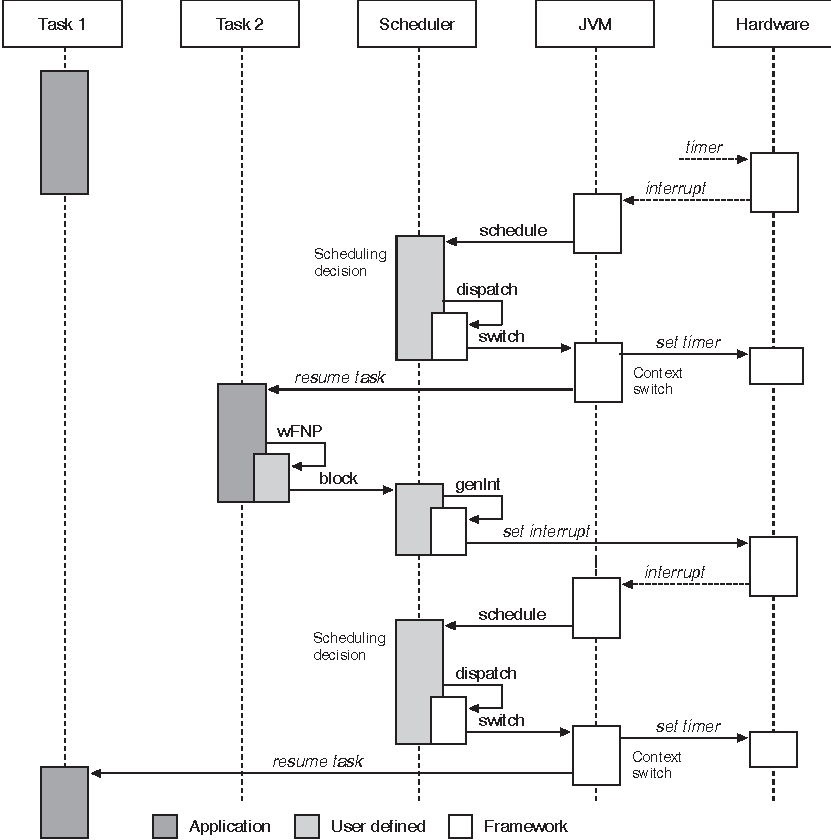
\includegraphics[scale=\picscale]{runtime/rt_user_interaction}
    \caption[Interaction diagram of the user scheduler framework]
    {Interaction and message exchange between the application,
the scheduler, the JVM and the hardware}
    \label{fig_arch_rt_user_interaction}
\end{figure*}

The first event is a timer event to unblock Task 2 for a new period.
The generated timer event results in a call of the user defined
scheduler. The scheduler performs its scheduling decision and issues
a context switch to Task 2. With every context switch the timer is
reprogrammed to generate an interrupt at the next time triggered
event for a higher priority task. Task 2 performs the periodic work
and ceases execution by invocation of \code{waitForNextPeriod()}.
The scheduler is called and requests an interrupt from the hardware
resulting in the same call sequence as with a timer or other
hardware interrupt. The software generated interrupt imposes
negligible overhead and results in a single entry point for the
scheduler. Task 1 is the only ready task in this example and is
resumed by the scheduler.

Using a general scheduling framework for a real-time scheduler is
not without its costs. Additional methods are invoked from a
scheduling event until the actual dispatch takes place. The context
switch is about 20\% slower than in the original implementation. It
is the opinion of the author that the additional cost is outweighed
by the flexibility of the framework.

\begin{lstlisting}[float,caption={Code fragment oft the application},
label=lst:arch:rt:user:app]
        for (;;) {
            doPeriodicWork();
            waitForNextPeriod();
        }
\end{lstlisting}

\begin{lstlisting}[float,caption={Implementation in RtThread},
label=lst:arch:rt:user:rtthr]
    public boolean waitForNextPeriod() {

        synchronized(monitor) {

            // ps is the instance of
            // the PriorityScheduler
            int nxt = ps.next[nr] + period;

            int now = Scheduler.getNow()
            if (nxt-now < 0) {
                // missed deadline
                doMissAction();
                return false;
            } else {
                // time for the next unblock
                ps.next[nr] = nxt;
            }
            // just schedule an interrupt
            // schedule() gets called.
            ps.block();
        }
        return true;
    }
\end{lstlisting}

\begin{lstlisting}[float,caption={Implementation of the PriorityScheduler},
label=lst:arch:rt:user:prsched]
    public void schedule() {

        // Find the ready thread with
        // the highest priority.
        int nr = getReady();

        // Search the list of sleeping threads
        // to find the nearest release time
        // in the future of a higher priority
        // thread than the one that will be
        // released now.
        int time = getNextTimer(nr);

        // This time is used for the next
        // timer interrupt.
        // Perform the context switch.
        dispatch(task[nr], time);
        // No access to locals after this point.
        // We are running in the NEW context!
    }
\end{lstlisting}


\subsection{Predictability}

The architecture of JOP is designed to simplify WCET analysis. Every
JVM bytecode maps to one ore more microcode instructions. Every
microcode instruction takes exactly one cycle to execute. Thus, the
execution time at the bytecode level is known cycle accurately. The
microcode contains no data dependent or unbound loops that would
compromise the WCET analysis (see Chapter~\ref{chap:wcet}).

The worst-case time for dispatching is known cycle accurately on
this architecture. Only the time behavior of the user scheduler
needs to be analyzed. With the known WCET of every bytecode, as
listed in Appendix~\ref{appx:bytecode}, the WCET of the scheduler
can be obtained by examining it at the bytecode level. This can be
done manually or with a WCET analysis tool.

\subsection{Related Work}

Several implementations of user-level schedulers in standard
operating systems have been proposed. In \cite{REDLinux2003}, the
Linux scheduling mechanism is enhanced. It is divided into a
dispatcher and an allocator. The dispatcher remains in kernel space;
while the allocator is implemented as a user space function. The
allocator transforms four basic scheduling parameters (priority,
start time, finish time and budget) into scheduling attributes to be
used by the dispatcher. Many existing schedulers can be supported
with this parameter set, but others that are based on different
parameters cannot be implemented. This solution does not address the
implementation of protocols for shared resources.

A different approach defines a new API to enable applications to use
application-defined scheduling in a way compatible with the
scheduling model defined in POSIX \cite{787339}. It is implemented
in the MaRTE OS, a minimal real-time kernel that provides the C and
Ada language POSIX interface. This interface has been submitted to
the Real-Time POSIX Working Group for consideration.

One approach to user-level scheduling in Java can be found in
\cite{Feizabadi:2003:UAS}. A thread \emph{multiplexor}, as part of
the FLEX ahead-of-time compiler system for Java, is used for utility
accrual scheduling. However, the underlying operating system -- in
this case Linux -- can still be seen through the framework and there
is no support for Java synchronization.

\subsection{Summary}

This section and Section~\ref{sec:rtprof} consider the
implementation of real-time scheduling on a Java processor. The
novelty of the described approach is in implementing functions
usually associated with an RTOS in Java. That means that real-time
Java is not based on an RTOS, and therefore not restricted to the
functionality provided by the RTOS. With JOP, a self-contained
real-time system in pure Java becomes possible. This system is
augmented with a framework to provide scheduling functions at the
application level. The implementation of the specification,
described in Section~\ref{sec:rtprof}, is successfully used as the
basis for a commercial real-time application in the railway
industry. Future work will extend this framework to support multiple
schedulers. A useful combination of schedulers would be: one for
standard \code{java.lang.Thread} (optimized for throughput), one for
soft real-time tasks and one for hard real-time tasks.

% rewrite scjava
    
\section{A Profile for Safety Critical Java}
\label{sec:scjava}

The proposed profile is an refinement of the profile described in
Section~\label{sec:rtprof}. Further development of applications on
JOP shall be based on this profile and the current applications
(e.g.\ \"OBB bg and Lift) should be migrated to this profile.

\emph{TODO: update with our ISROC 2007 paper and remove Jan's text.}

\section{Safety Critical Java}

Puschner and Wellings were the first to consider the concerns of
safety- and mission-critical systems in the context of the RTSJ for
Java~\cite{Pusch01}. Their proposal adopts the approach pioneered by
the Ravenscar tasking profile for Ada~\cite{697453} which defined a
strict subset of the Ada language for high-integrity systems.  This
work was later refined by Schoeberl et al.~\cite{jop:scjava}.

In this paper we focus on the Safety Critical Java (SCJ)
specification, a new standard for safety critical applications which
is being drafted by the JSR 302 expert group.

%%%
We should note that JSR 302 has not been finalized, thus our
presentation gives an overview of work in progress. Furthemore, our
proposal of real-time garbage collection to SCJ is an extension of
the proposed standard.


This draft JSR 302 standard, like previous work, defines a strict
subset of the RTSJ which is intended to provide a programming model
suited to a large class of safety critical applications. Restricting
the features of the RTSJ is intended to make programs more amenable
to worst case analysis and manual or automatic validation. The SCJ
is structured in three increasingly expressive levels: Level 0
restricts applications to a single threaded cyclic executive, level
1 assumes a single ``mission'' with a static thread assignment, and
level 2 is a multi-mission model with dynamic thread creation. This
paper focuses on level 1 which is expected to cover a large number
of existing SC applications. It should be noted that while all
levels are designed to run on a vanilla RTSJ VM, it is expected that
vendors will provided implementations that are optimized for the
particular features of each level.


\begin{figure}[t!]
{\small
\begin{verbatim}
package javax.safetycritical;

public abstract class RealtimeThread {

    protected RealtimeThread(RelativeTime period,
        RelativeTime deadline,
        RelativeTime offset, int memSize)

    protected RealtimeThread(String event,
        RelativeTime minInterval,
        RelativeTime deadline, int memSize)

    abstract protected boolean run();

    protected boolean cleanup() {
        return true;
    }
}

public abstract class PeriodicThread
        extends RealtimeThread {

    public PeriodicThread(RelativeTime period,
        RelativeTime deadline,
        RelativeTime offset, int memSize)

    public PeriodicThread(RelativeTime period)
}
\end{verbatim} }
\caption{Periodic thread definition for SCJ}\label{lst:scjdef}
\end{figure}

\subsection{SCJ Level 1}

Level 1 of the SCJ requires that all threads be defined during an
initial \emph{initialization} phase. This phase is run only once at
virtual machine startup. The second phase, called the \emph{mission}
phase, begins only when all threads have been started. This phase
runs until virtual machine shutdown. Level 1 supports only two kinds
of schedulable objects: periodic threads and sporadic events. The
latter can be generated by either hardware or software. This
restrictions keeps the schedulability analysis simple. In SCJ
priority ceiling emulation is the default monitor control policy.
The default ceiling is top priority.

The Java \code{wait} and \code{notify} primitives are not allowed in
SCJ level 0 and 1. This further simplifies analysis. The consequence
is that a thread context switch can only occur if a higher priority
thread is released or if the current running thread yields (in the
case of SCJ by returning from the \code{run()} method).

In the RTSJ, periodic tasks are expressed by unbounded loops with,
at some point, a call to the \code{waitForNextPeriod()} (or
\code{wFNP()} for short) method of class \code{RealtimeThread}. This
has the effect of yielding control to the scheduler which will only
wake the thread when its next period starts or shortly thereafter.
In SCJ, as a simplification, periodic logic is encapsulated in a
\code{run()} method which is invoked at the start of every period of
a given schedulable object. When the thread returns from
\code{run()} it is blocked until the next period.

Figure~\ref{lst:scjdef} shows part of the definition of the SCJ
thread classes from \cite{jop:scjava}\footnote{These are similar to
the draft JSR
  302 class definitions, but as the specification is still in the process of
  being finalized we choose to use the classes available in the
  infrastructure we use for our implementation.}. Figure~\ref{lst:per} shows
the code for a periodic thread. This class has only one \code{run()}
method which performs a periodic computation.

The loop construct with \code{wFNP()} is not used. The main
intention to avoid the loop construct, with the possibility to split
application logic into \emph{mini} phases, is simplification of the
WCET analysis. Only a single method has to be analyzed per thread
instead of all possible control flow path between \code{wFNP()}
invocations.

\begin{figure}[!t]
{\small
\begin{verbatim}
new PeriodicThread(
    new RelativeTime(...)) {

        protected boolean run() {
            doPeriodicWork();
            return true;
        }
};
\end{verbatim} }
    \caption{A periodic application thread in SCJ}
    \label{lst:per}
\end{figure}

\begin{figure}[!t]
{\small
\begin{verbatim}
    public void run() {

        State local = new State();
        doSomeInit();
        local.setA();
        waitForNextPeriod();

        for (;;) {
            while (!switchToB()) {
                doModeAwork();
                waitForNextPeriod();
            }
            local.setB();
            while (!switchToA()) {
                doModeBWork();
                waitForNextPeriod();
            }
            local.setA();
        }
    }
\end{verbatim} }
    \caption{Possible logic for a periodic thread in the RTSJ}\label{lst:rtsj:per}
\end{figure}


We contrast the SCJ threading with Figure~\ref{lst:rtsj:per} where a
periodic RTSJ thread is shown. Suspension of the thread to wait for
the next period is performed by an explicit invocation of
\code{wFNP()}. The coding style in this example makes analysis of
the code more difficult than necessary. First the initialization
logic is mixed with the code of the mission phase, this means that a
static analysis may be required to discover the boundary between the
startup code and the periodic behavior. The code also performs mode
switches with calls to \code{wFNP()} embedded in the logic. This
makes the worst case analysis more complex as calls to \code{wFNP()}
may occur anywhere and require deep understanding of feasible
control flow paths.  Another issue, which does not affect
correctness, is the fact that object references can be preserved in
local variables across calls to \code{wFNP()}. As we will see later
this has implications for the GC.

\clearpage
    \section{JVM Architecture}

This section presents the details of the implementation of the JVM
on JOP. The representation of objects and the stack frame is chosen
to support JOP as processor for real-time systems. However, since
the data structures are realized through microcode they can be
easily changed for a system with different needs. For example: to
simplify a compacting GC a handle to an object can be implemented by
changing the microcode of \code{getfield}, \code{putfield} and
\code{new}.

\subsection{Runtime Data Structures}

Memory is addressed as 32-bit data, which means that memory pointers
are incremented for every four bytes. No single byte or 16-bit
access is necessary. The abstract type reference is a pointer to
memory that represents the object or an array. The reference is
pushed on the stack before an instruction can operate on it. A null
reference is represented by the value 0.

\subsubsection{Stack Frame}

On invocation of a method, the invoker's context is saved in a newly
allocated frame on the stack. It is restored when the method
returns. The saved context consists of following registers:

\begin{description}

\item[SP:] Immediately before invocation the stack pointer points to
the last argument for the called function. This value is reduced by
the argument count (i.e. the arguments are consumed) and saved in
the new stack frame.

\item[PC:] The pointer to the next bytecode instruction after the invoke
instruction.

\item[VP:] The pointer to the memory area on the stack that contains
the locals.

\item[CP:] The pointer to the constant pool of the class from the invoking
method.

\item[MP:] The pointer to the method structure of the invoking method.

\end{description}

SP, PC and VP are registers in JOP while CP and MP are local
variables of the JVM. \figurename~\ref{fig_jvm_stack_invoke}
provides an example of the stack before and after invoking a method.
In this example, the called method has two arguments and contains
two local variables. If the method is a virtual one, the first
argument is the reference to the object (the \emph{this}-pointer).
The arguments implicit become locals in the called method and are
accessed in the same way as local variables. The start of the stack
frame (\emph{Frame} in the figure) needs not to be saved. It is not
needed during execution of the method or on return. To access the
starting address of the frame (e.g. for an exception) it can be
calculated with information from the method structure:

\[Frame = VP + arg\_cnt + locals\_cnt\]

\begin{figure}
    \centering
    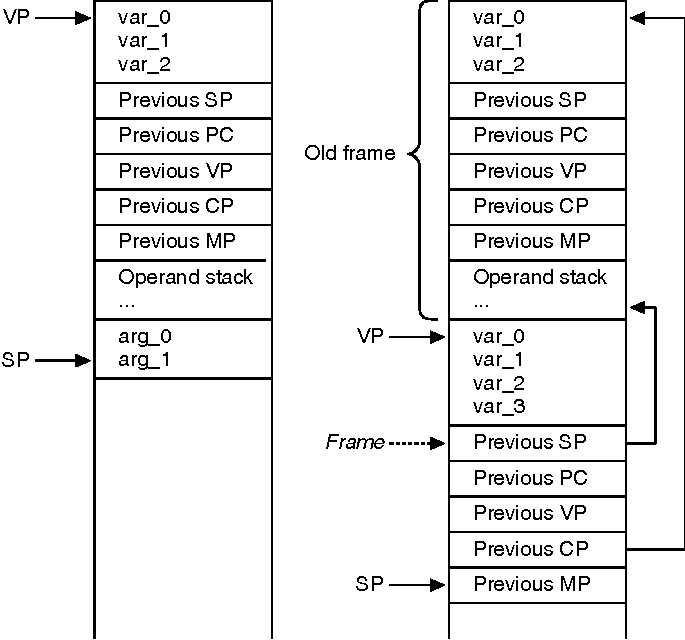
\includegraphics[scale=\picscale]{jvm/jvm_stack_invocation}
    \caption{Stack change on method invocation}
    \label{fig_jvm_stack_invoke}
\end{figure}

\subsubsection{Object Layout}

\figurename~\ref{fig_jvm_object} shows the representation of an
object in memory. The object reference points to the first instance
variable of the object. At the offset $-1$, a pointer is located to
access class information. To speed-up method invocation, it points
directly to the method table of the objects class instead of the
beginning of the class data. With the GC the object is accessed via
one indirection, the handle (see Chapter~\ref{chap:rtgc}). The
pointer to the method vector base if part of the handle.

\begin{figure}
    \centering
    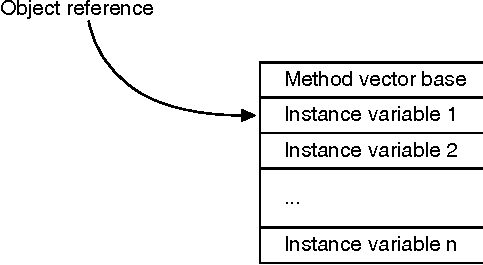
\includegraphics[scale=\picscale]{jvm/jvm_object}
    \caption{Object format}
    \label{fig_jvm_object}
\end{figure}

\subsubsection{Array Layout}

\figurename~\ref{fig_jvm_array} shows the representation of an array
in memory. The object reference points to the first element of the
array. At the offset $-1$, the length of the array can be found.
With the GC the array is accessed via one indirection, the handle
(see Chapter~\ref{chap:rtgc}). The size fields is part of the
handle.

\begin{figure}
    \centering
    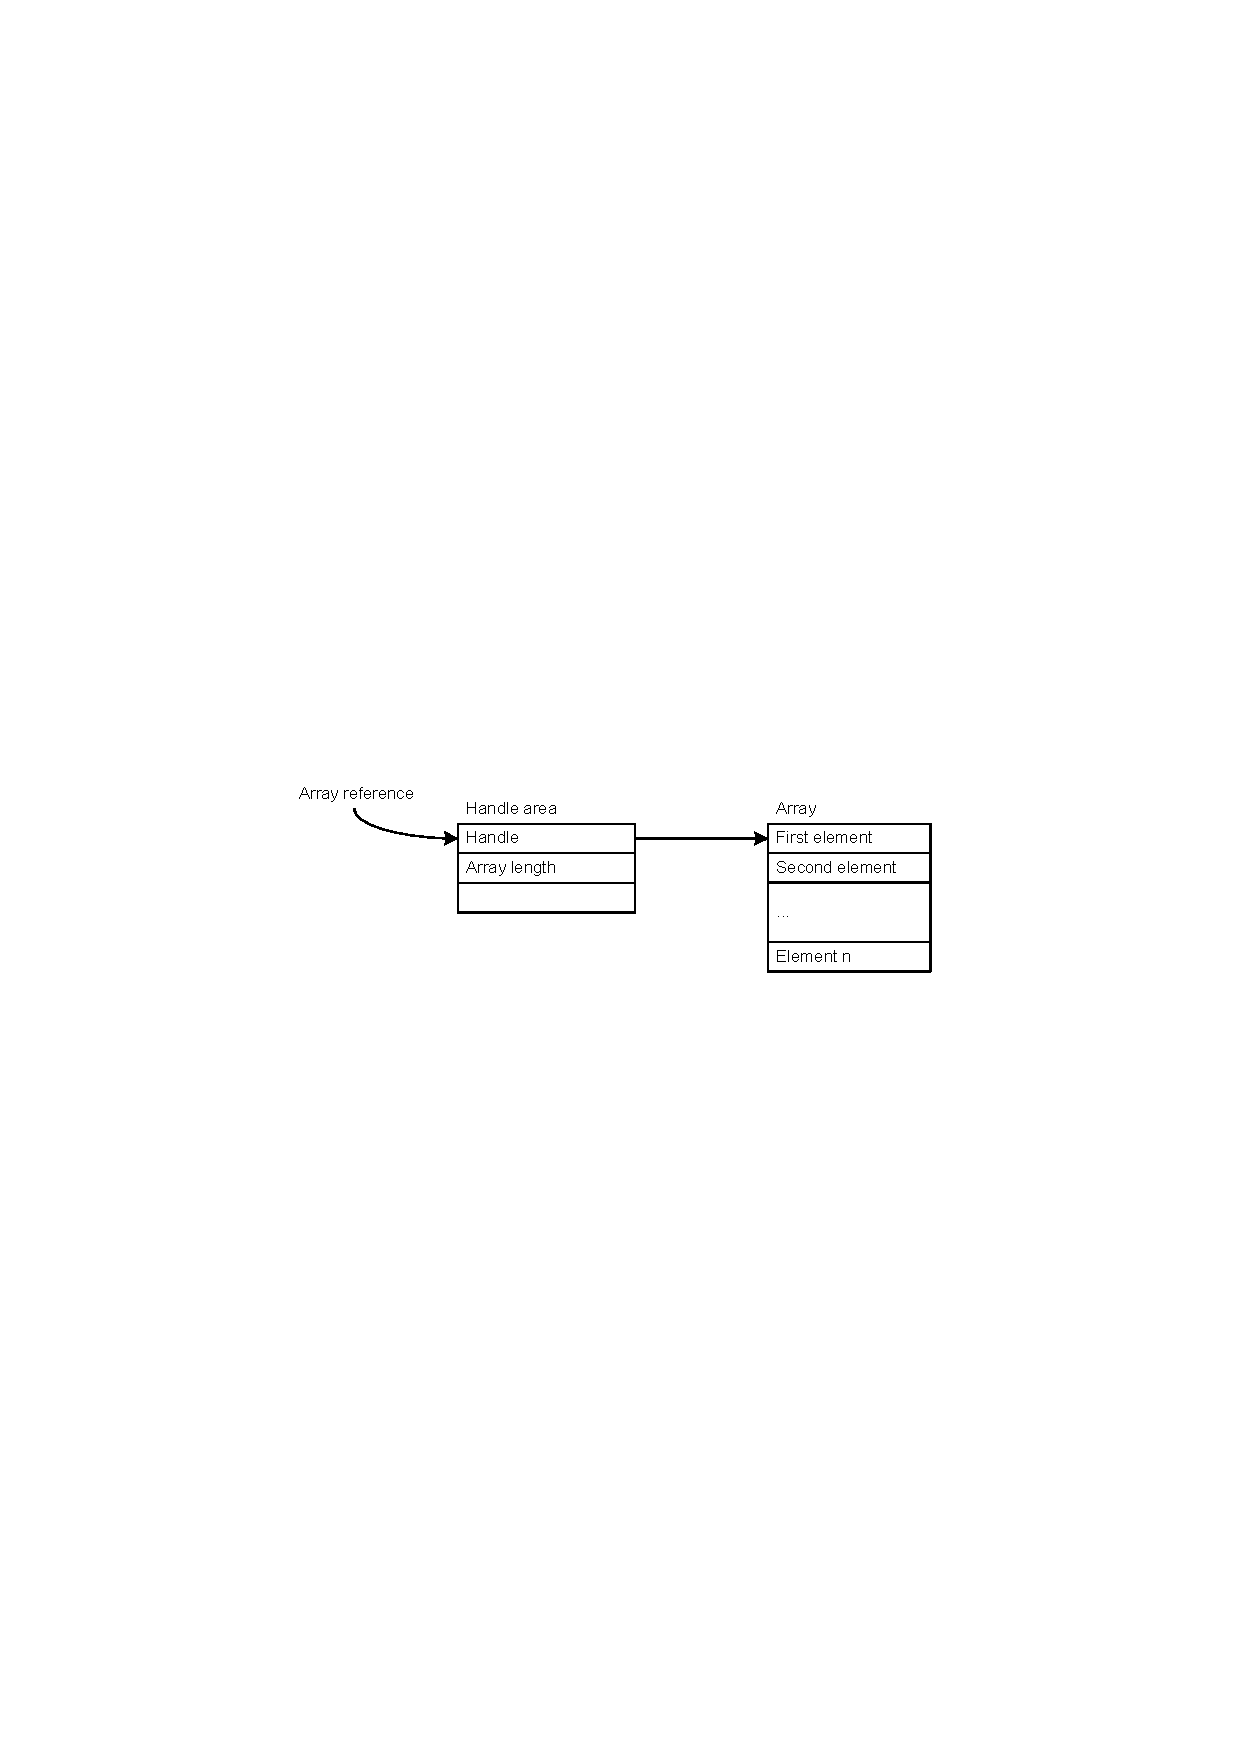
\includegraphics[scale=\picscale]{jvm/jvm_array}
    \caption{Array format}
    \label{fig_jvm_array}
\end{figure}


\subsubsection{Class Structure}

Runtime class information, as shown in Figure~\ref{fig_jvm_class},
consists of the class variables, the dispatch table for the methods,
the constant pool and an optional interface table.

\begin{figure}
    \centering
    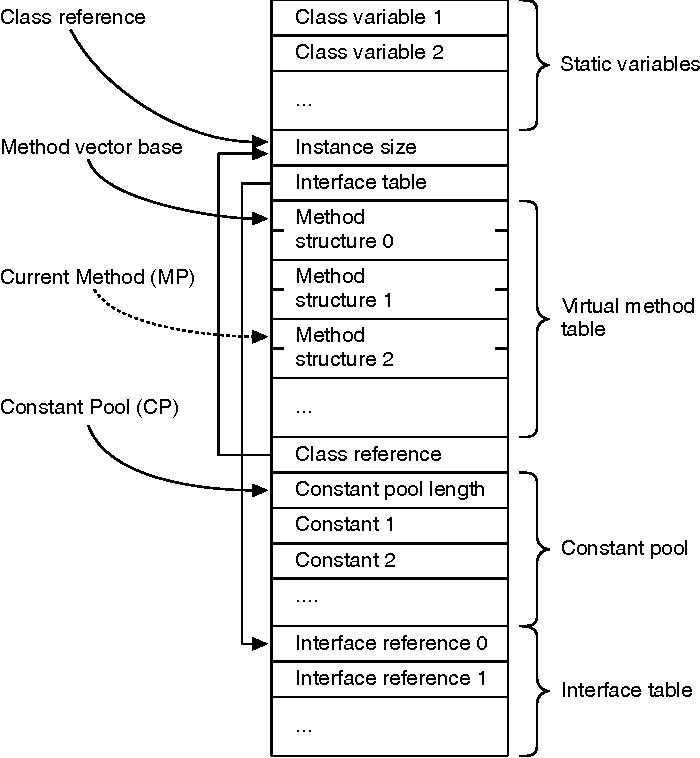
\includegraphics[scale=\picscale]{jvm/jvm_class}
    \caption{Runtime class structure}
    \label{fig_jvm_class}
\end{figure}


The class reference is obtained from the constant pool when a new
object is created. The method vector base pointer is a reference
from an object to its class (see Figure~\ref{fig_jvm_object}). It is
used on \code{invokevirtual} with an index retrieved from the
constant pool. A pointer to the method structure of the current
method is saved in the JVM variable MP. The method structure, as
shown in Figure~\ref{fig_jvm_method}, contains the starting address
and length of the method (in 32-bit words), argument and local
variable count and a pointer to the constant pool of the class.
Since the constant pool is an often accessed memory area, a pointer
to it is kept in the JVM variable CP.

\begin{figure*}
    \centering
    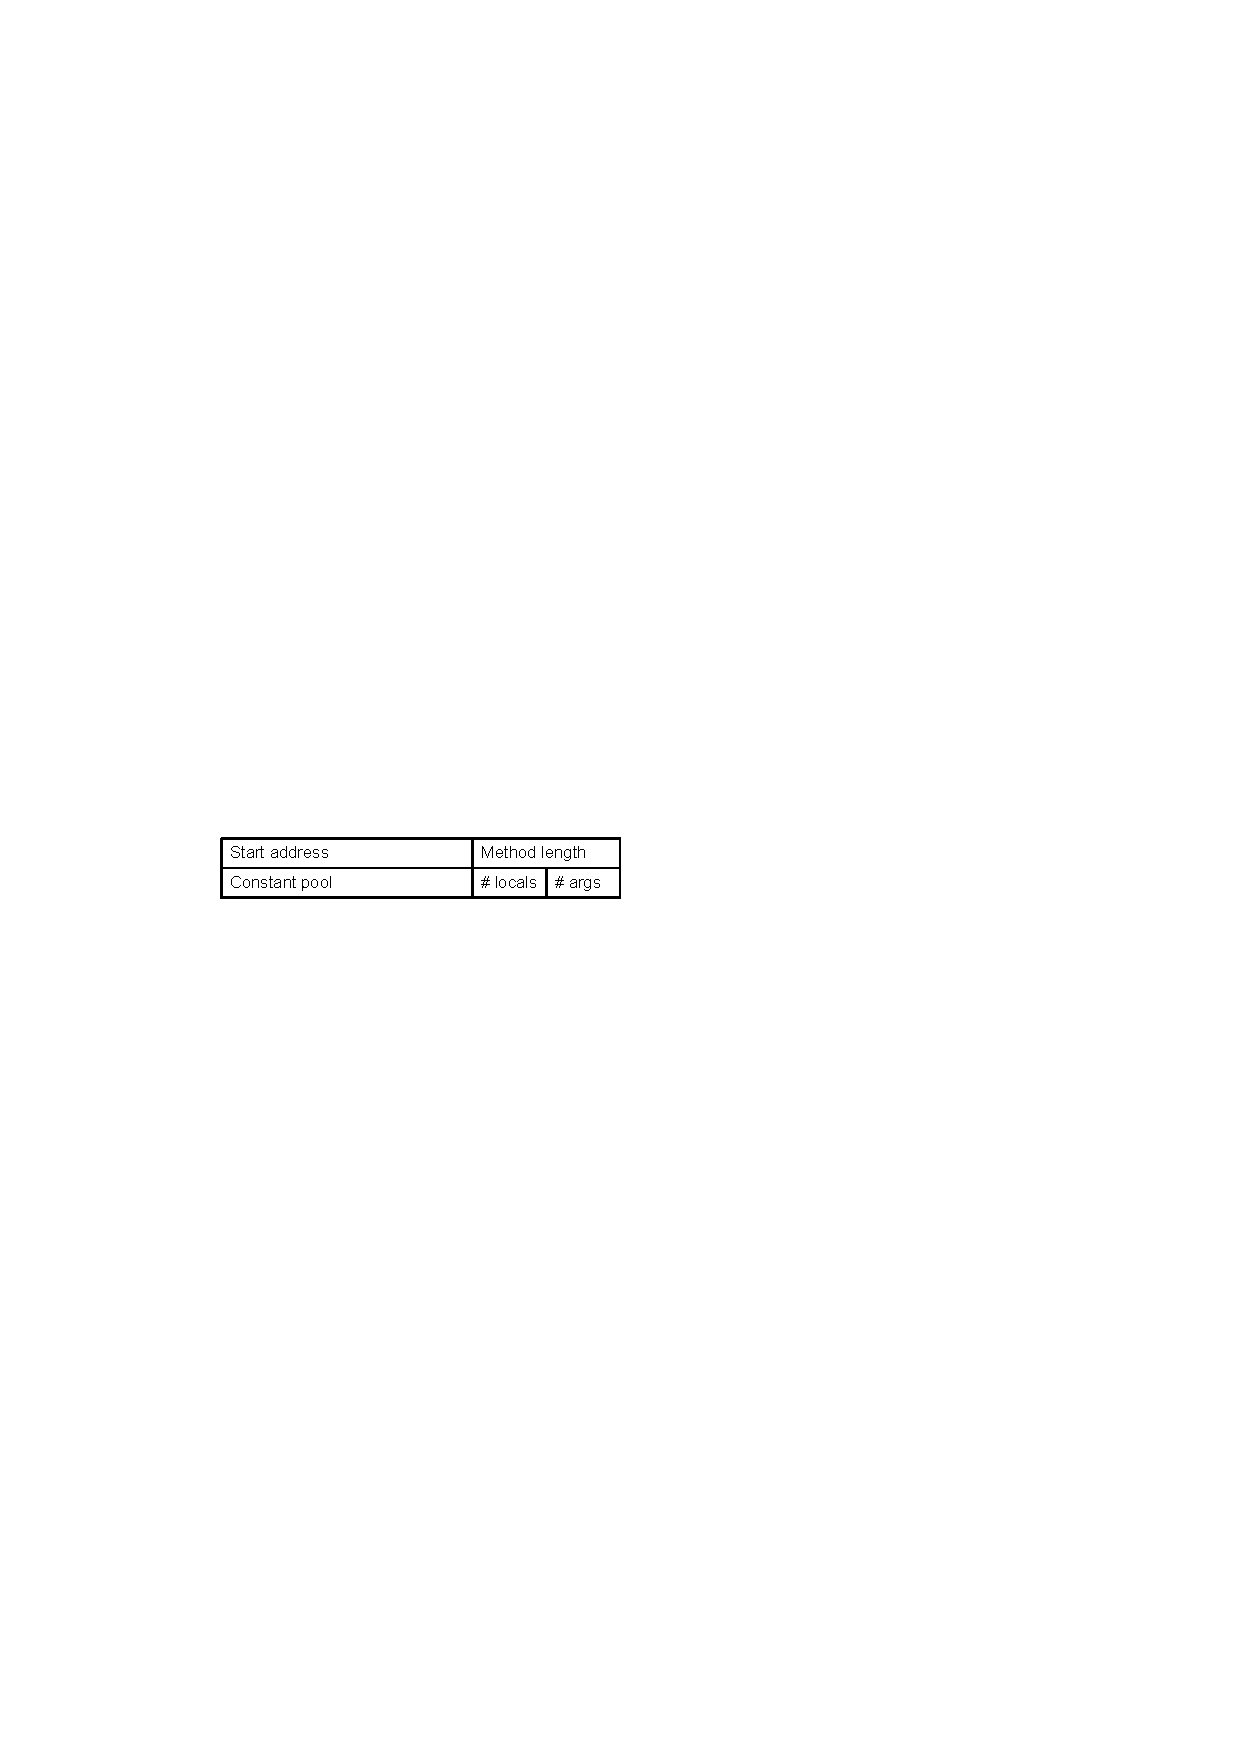
\includegraphics[scale=\picscale]{jvm/jvm_method}
    \caption{Method structure}
    \label{fig_jvm_method}
\end{figure*}


The interface table contains references to the method structures of
the implementation. Only classes that implement an interface contain
this table. To avoid searching the class hierarchy on
\code{invokeinterface}, each interface method is assigned a unique
index. This provides constant execution time, but can lead to large
interface tables.

The constant pool contains various constants of a class. The entry
at index 0 is the length of the pool. All constants, which are
symbolic in the class files, are resolved on class loading or during
pre-linking. The different constant types and their values after
resolving are listed in \tablename~\ref{tab_jvm_const_pool}. The
names for the types are the same as in the JVM specification
\cite{jvm}.


\begin{table}[htbp]
    \centering
    \begin{tabular}{ll}
        \toprule
        Constant type &  Description \\
        \midrule
        Class &  A pointer to a class (class reference) \\
        Fieldref &   For static fields: a direct pointer to the field \\
                &   For object fields: the position relative to the object \\
                & reference \\
        Methodref &  For static methods: a direct pointer to the method structure \\
                & For virtual methods: the offset in the method table \\
                & (= index*2) and the number of arguments \\
        InterfaceMethodref &  A system wide unique index into the interface table \\
        String  & A pointer to the string object that represents the string \\
                & constant \\
        Integer & The constant value \\
        Float   & The constant value \\
        Long    & This constant value spans two entries in the constant pool \\
        Double  & Same as for long constants \\
        NameAndType & Not used \\
        Utf8    & Not used \\
        \bottomrule
    \end{tabular}
    \caption{Constant pool entries}
    \label{tab_jvm_const_pool}
\end{table}

    \subsection{Booting the JVM}

\index{JVM!boot-up}

One interesting issue for an embedded system is how the boot-up is
performed. On power-up, the FPGA starts the configuration state
machine to read the FPGA configuration data either from a Flash or
via a download cable (for development). When the configuration has
finished, an internal reset is generated. After that reset, microcode
instructions are executed starting from address 0. At this stage, we
have not yet loaded any application program (Java bytecode). The
first sequence in microcode performs this task. The Java application
can be loaded from an external Flash or via a serial line (or an USB
port) from a PC. The microcode assembly configured the mode.
Consequently, the Java application is loaded into the main memory. To
simplify the startup code we perform the rest of the startup in Java
itself, even when some parts of the JVM are not yet setup.

In the next step, a minimal stack frame is generated and the special
method \code{Startup.boot()} is invoked. From now on JOP runs in
Java mode. The method \code{boot()} performs the following steps:
\begin{samepage}
\begin{enumerate}
    \item Send a greeting message to \emph{stdout}
    \item Detect the size of the main memory
    \item Initialize the data structures for the garbage collector
    \item Initialize \code{java.lang.System}
    \item Print out JOP's version number, detected clock speed, and
    memory size
    \item Invoke the static class initializers in a predefined order
    \item Invoke the \code{main} method of the application class
\end{enumerate}
\end{samepage}


\chapter{Real-Time Garbage Collection}
\label{chap:rtgc}
    Automatic memory management or garbage collection greatly simplifies
development of large systems. However, garbage collection is usually
not used in real-time systems due to the unpredictable temporal
behavior of current implementations of a garbage collector. In this
chapter we describe a concurrent collector that is scheduled
periodically in the same way as ordinary application threads. We
provide an upper bound for the collector period so that the
application threads will never run out of memory. This chapter is
based on the published papers \cite{jop:rtgc_sched} and
\cite{jop:scjgc}.


\section{Introduction}

Garbage Collection (GC) is an essential part of the Java runtime
system. GC enables automatic dynamic memory management which is
essential to build large applications. Automatic memory management
frees the programmer from complex and error prone explicit memory
management (\code{malloc} and \code{free}).

However, garbage collection is considered unsuitable for real-time
systems due to the unpredictable blocking times introduced by the GC
work. One solution, used in the Real-Time Specification for Java
(RTSJ) \cite{rtsj}, introduces new thread types with program-managed,
scoped memory for dynamic memory requirements. This scoped memory
(and static memory called \emph{immortal} memory) is not managed by
the GC, and strict assignment rules between different memory areas
have to be checked at runtime. This programming model differs largely
from standard Java and is difficult to use \cite{Niessner03,
conf/isorc/PizloFHV04}.

We believe that for the acceptance of Java for real-time systems, the
restrictions imposed by the RTSJ are too strong. To simplify creation
of possible large real-time applications, most of the code should be
able to use the GC managed heap. For a collector to be used in
real-time systems two points are essential:
\begin{itemize}
    \item The GC has to be incremental with a short maximum blocking time
    that has to be known
    \item The GC has to keep up with the garbage generated by the
    application threads to avoid out-of-memory stalls
\end{itemize}
The first point is necessary to limit interference between the GC
thread and high-priority threads. It is also essential to minimize
the overhead introduced by read- and write-barriers, which are
necessary for synchronization between the GC thread and the
application threads. The design of a GC within these constraints is
the topic of this chapter.

The second issue that has to be considered is scheduling the GC so
that the GC collects enough garbage. The memory demands (static and
dynamic) by the application threads have to be analyzed. These
requirements, together with the properties of the GC, result in
scheduling parameters for the GC thread. We will provide a solution
to calculate the maximum period of the GC thread that will collect
enough memory in each collector cycle so we will never run out of
memory. The collector cycle depends on the heap size and the
allocation rate of the application threads.

To distinguish between other garbage collectors and a collector for
(hard) real-time systems we define a real-time collector as follows:

\begin{quote}
    A real-time garbage collector provides time predictable
    automatic memory management for tasks with a bounded memory
    allocation rate with minimal temporal interference to tasks
    that use only static memory.
\end{quote}


The collector presented in this chapter is based on the work by
Steele \cite{gc:steele75},  Dijkstra \cite{gc:dijkstra78} and Baker
\cite{gc:baker78}. However, the copying collector is changed to
perform the copy of an object concurrently by the collector and not
as part of the mutator work. Therefore we name it
\emph{concurrent-copy} collector.

We will use the terms first introduced by Dijkstra with his
\emph{On-the-Fly} concurrent collector. The application is called the
\emph{mutator} to reinforce that the application changes (mutates)
the object graph while the GC does the collection work. The GC
process is simply called \emph{collector}. In the following
discussion we will use the color scheme of white, gray, and black
objects as introduced by Dijkstra with his \emph{On-the-Fly}
concurrent collector.

\begin{description}
    \item[Black] indicates that the object and all immediate
    descendants have been visited by the collector.
    \item[Grey] objects have been visited, but the descendants may
    not have been visited by the collector, or the mutator has
    changed the object.
    \item[White] objects are unvisited. At the beginning of a GC
        cycle all objects are white. At the end of the tracing,
        all white objects are garbage.
\end{description}

At the end of a collection cycle all black objects are live (or
floating garbage) and all white objects are garbage.

\subsection{Incremental Collection}

An incremental collector can be realized in two ways: either by doing
part of the work on each allocation of a new object or by running the
collector as an independent process. For a single-threaded
application, the first method is simpler as less synchronization
between the application and the collector is necessary. For a
multi-threaded environment there is no advantage by interleaving
collector work with object allocation. In this case we need
synchronization between the collector work done by one thread and the
manipulation of the object graph performed by the other mutator
thread. Therefore we will consider a concurrent solution where the
collector runs in its own thread or processor. It is even possible to
realize the collector as dedicated hardware \cite{gc:flavius}.

\subsection{Conservatism}

Incremental collector algorithms are conservative, meaning that
objects becoming unreachable during collection are not collected by
the collector --- they are floating garbage. Many approaches exist
to reduce this conservatism in the general case. However, algorithms
that completely avoid floating garbage are impractical. For
different conservative collectors the worst-case bounds are all the
same (i.e., all objects that become unreachable remain floating
garbage). Therefore the level of conservatism is not an issue for
real-time collectors.

\subsection{Safety Critical Java}

In Section~\ref{sec:scjava} a profile for safety critical Java (SCJ)
is defined. SCJ has two interesting properties that may simplify the
implementation of a real-time collector. Firstly, the split between
initialization and mission phase, and secondly the simplified
threading model (which also mandates that self-blocking operations
are illegal in mission).  During initialization of the application a
SCJ virtual machine does not have to meet any real-time constraints
(other than possibly a worst case bound on the entire initialization
phase). It is perfectly acceptable to use a non-real-time GC
implementation during this phase -- even a stop-the-world GC. As the
change from initialization to mission phase is explicit, it is clear
when the virtual machine must initiate real-time collection and
which code runs during the mission phase.


Simplifying the threading model has the following advantage, if the
collector thread runs at a lower priority than all other threads in
the system, it is the case that when it runs \emph{all} other threads
have returned from their calls to \code{run()}. This is trivially
true due to the priority preemptive scheduling discipline\footnote{If
we would allow blocking in the application threads, we would also
need to block the GC thread.}. Any thread that has not returned from
its \code{run()} method will preempt the GC until it returns. This
has the side effect that the GC will never see a root in the call
stack of another thread. Therefore, the usually atomic operation of
scanning call stacks can be omitted in the mission phase. We will
elaborate on this in Section~\ref{sec:scj:simple}.


\section{Scheduling of the Collector Thread}
\label{sec:gcsched}

The collector work can be scheduled either \emph{work} based or
\emph{time} based. On a work based scheduling, as performed in
\cite{gc:siebert:phd}, an incremental part of the collector work is
performed at object allocation. This approach sounds quite natural
as threads that allocate more objects have to pay for the collector
work. Furthermore, no additional collector thread is necessary. The
main issue with this approach is to determine how much work has to
be done on each allocation -- a non trivial question as collection
work consists of different phases. A more subtle question is: Why
should a high frequency (and high priority) thread increase its WCET
by performing collector work that does not have to be done at that
period? Leaving the collector work to a thread with a longer period
will allow higher utilization of the system.

On a time based scheduling of the collector work, the collector runs
in its own thread. Scheduling this thread as a \emph{normal}
real-time thread is quite natural for a hard real-time system. The
question is: which priority to assign to the collector thread? The
Metronome collector \cite{gc:bacon03} uses the highest priority for
the collector. Robertz and Henriksson \cite{780745} and Schoeberl
\cite{jop:rtgc_sched} argue for the lowest priority. When building
hard real-time systems the answer must take scheduling theory into
consideration: the priority is assigned according to the period,
either rate monotonic \cite{321743} or more general deadline
monotonic \cite{Audsley-etal91}. Assuming that the period of the
collector is the longest in the system and the deadline equals the
period the collector gets the lowest priority.

In this section we provide an upper bound for the collector period
so that the application threads will never run out of memory. The
collector period, besides the WCET of the collector, is the single
parameter of the collector that can be incorporated in standard
schedulability analysis.

The following symbols are used in this section: heap size for a
mark-compact collector ($H_{MC}$) and for a concurrent-copying
collector ($H_{CC}$) containing both semi-spaces, period of the GC
thread ($T_{GC}$), period of a single mutator thread ($T_M$), period
of mutator thread $i$ ($T_i$) from a set of threads, and memory
amount allocated by a single mutator ($a$) or by mutator $i$ ($a_i$)
from a set of threads.

We assume that the mutator allocates all memory at the start of the
period and the memory becomes garbage at the end. In other words the
memory is live for one period. This is the worst-case\footnote{See
Section~\ref{sec:wc:live} for an example where the worst-case
lifetime is two periods.}, but very common as we can see in the
following code fragment.
\begin{samepage}
\begin{lstlisting}
    for (;;) {
        Node n = new Node();
        work(n);
        waitForNextPeriod();
    }
\end{lstlisting}
\end{samepage}
The object \code{Node} is allocated at the start of the period and
\code{n} will reference it until the next period when a new
\code{Node} is created and assigned to \code{n}. In this example we
assume that no reference to \code{Node} is stored (inside
\code{work}) to an object with longer lifetime.




\subsection{An Example} \label{sec:example}

\begin{figure}
\begin{center}
    \input{jvm/exmc.latex}
    \caption{Heap usage during a mark-compact collection cycle}
\label{fig:exmc}
\end{center}
\end{figure}

\begin{figure}
\begin{center}
    \input{jvm/excc2.latex}
    \caption{Heap usage during a concurrent-copy collection cycle}
\label{fig:excc}
\end{center}
\end{figure}


We start our discussion with a simple example\footnote{The relation
between the heap size and the mutator/collector proportion is an
arbitrary value in this example. We will provide the exact values in
the next sections.} where the collector period is 3 times the mutator
period ($T_{GC} = 3 T_M$) and a heap size of 8 objects ($8a$). We
show the heap during one GC cycle for a mark-compact and a
concurrent-copy collector. The following letters are used to show the
status of a memory cell (that contains one object from the mutator in
this example) in the heap: $g_i$ is garbage from mutator cycle $i$,
$l$ is the live memory, and $f$ is floating garbage. We assume that
all objects that become unreachable during the collection remain
floating garbage.

Figure~\ref{fig:exmc} shows the changes in the heap during one
collection cycle. At the start there are three objects ($g_1$,
$g_2$, and $g_3$) left over from the last cycle (floating garbage)
which are collected by the current cycle and one live object $l_4$.
During the collection the live objects become unreachable and are
now floating garbage (e.g. $f_4$ in the second sub-figure). At the
end of the cycle, just before compacting, we have three garbage
cells ($g_1$-$g_3$), three floating garbage cells ($f_4$-$f_6$) and
one live cell $l_7$. Compaction moves the floating garbage and the
live cell to the start of the heap and we end up with four free
cells. The floating garbage will become garbage in the next
collection cycle and we start over with the first sub-figure with
three garbage cells and one live cell.

Figure~\ref{fig:excc} shows one collection cycle of the
concurrent-copy collector. We have two memory spaces: the
\emph{from-space} and the \emph{to-space}. Again we start the
collection cycle with one live cell and three garbage cells left over
from the last cycle. Note that the order of the cells is different
from the previous example. New cells are allocated in the to-space
from the top of the heap, whereas moved cells are allocated from the
bottom of the heap. The second sub-figure shows a snapshot of the
heap during the collection: formerly live object $l_4$ is already
floating garbage $f_4$ and copied into to-space. A new cell $l_5$ is
allocated in the to-space. Before the flip of the two semi-spaces the
from-space contains the three garbage cells ($g_1$-$g_3$) and the
to-space the three floating garbage cells ($f_4$-$f_6$) and one live
cell $l_7$. The last sub-figure shows the heap after the flip: The
from-space contains the three floating cells which will be garbage
cells in the next cycle and the one live cell. The to-space is now
empty.

From this example we see that the necessary heap size for a
mark-compact collector is similar to the heap size for a copying
collector. We also see that the compacting collector has to move
more cells (all floating garbage cells and the live cell) than the
copying collector (just the one cell that is live at the beginning
of the collection).


\subsection{Minimum Heap Size} \label{sec:min:heap}

In this section we show the memory bounds for a mark-compact
collector with a single heap memory and a concurrent-copying
collector with the two spaces \emph{from-space} and \emph{to-space}.

The following symbols are used for the rest of the paper: heap size
for a mark-compact collector ($H_{MC}$) and for a concurrent-copying
collector ($H_{CC}$) containing both semi-spaces, period of the GC
thread ($T_{GC}$), period of a single mutator thread ($T_M$), period
of mutator thread $i$ ($T_i$) from a set of threads, and memory
amount allocated by a single mutator ($a$) or by mutator $i$ ($a_i$)
from a set of threads.

\subsubsection{Mark-Compact} \label{sec:gcsched:mc}

For the mark-compact collector, the heap $H_{MC}$ can be divided into
allocated memory $M$ and free memory $F$
%
\begin{equation}\label{equ:mcheap}
    H_{MC} = M + F = G + \overline{G} + L + F
\end{equation}
%
where $G$ is garbage at the start of the collector cycle that will
be reclaimed by the collector. Objects that become unreachable
during the collection cycle and will not be reclaimed are floating
garbage $\overline{G}$. These objects will be detected in the next
collection cycle. We assume the worst case that all objects that die
during the collection cycle will not be detected and therefore are
floating garbage. $L$ denotes all live,i.e.\  reachable, objects.
$F$ is the remaining free space.

We have to show that we will never run out of memory during a
collection cycle ($F\ge0$). The amount of allocated memory $M$ has to
be less than or equal to the heap size $H_{MC}$

\begin{equation}\label{equ:mcheapmin}
    H_{MC} \ge M = G + \overline{G} + L
\end{equation}


In the following proof the superscript $n$ denotes the collection
cycle. The subscript letters $S$ and $E$ denote the value at the
start and the end of the cycle, respectively.

\begin{lemma}

For a collection cycle the amount of allocated memory $M$ is bounded
by the maximum live data $L_{max}$ at the start of the collection
cycle and two times $A_{max}$, the maximum data allocated by the
mutator during the collection cycle.

\begin{equation}\label{equ:mc:lemma}
    M \le L_{max} + 2 A_{max}
\end{equation}

\end{lemma}

\begin{proof}

During a collection cycle $G$ remains constant. All live data that
becomes unreachable will be floating garbage. Floating garbage
$\overline{G}_E$ at the end of cycle $n$ will be detected (as
garbage $G$) in cycle $n+1$.
%
\begin{equation}\label{equ:flg}
    G^{n+1} = \overline{G}_E^n
\end{equation}
%
The mutator allocates $A$ memory and transforms part of this memory
and part of the live data at the start $L_S$ to floating garbage
$\overline{G}_E$ at the end of the cycle. $L_E$ is the data that is
still reachable at the end of the cycle.
%
\begin{equation}\label{equ:trans}
    L_S + A = L_E + \overline{G}_E
\end{equation}
%
with $A \le A_{max}$ and $L_S \le L_{max}$. A new collection-cycle
start immediately follows the end of the former cycle. Therefore the
live data remains unchanged.
%
\begin{equation}\label{equ:ldata}
    L_S^{n+1} = L_E^{n}
\end{equation}

We will show that (\ref{equ:mc:lemma}) is true for cycle 1. At the
start of the first cycle we have no garbage ($G=0$) and no live data
($L_S=0$). The heap contains only free memory.
%
\begin{equation}\label{equ:mc:start}
    M_S^1 = 0
\end{equation}
%
During the collection cycle the mutator allocates $A^1$ memory. Part
of this memory will be live at the end and the remaining will be
floating garbage.
%
\begin{equation}\label{equ:mc:cyc1:A}
    A^1 = L_E^1 + \overline{G}_E^1
\end{equation}
%
Therefore at the end of the first cycle
%
\begin{align}
\nonumber
    M_E^1 & = L_E^1 + \overline{G}_E^1\\
    M^1   & = A^1
\end{align}
%
As $A^1 \le A_{max}$ (\ref{equ:mc:lemma}) is fulfilled for cycle 1.

Under the assumption that (\ref{equ:mc:lemma}) is true for cycle
$n$, we have to show that (\ref{equ:mc:lemma}) holds for cycle
$n+1$.

\begin{equation}
    M^{n+1} \le L_{max} + 2 A_{max}
\end{equation}

\begin{align}
    M^n & = G^n + \overline{G}_E^n + L_E^n\\
    M^{n+1} & = G^{n+1} + \overline{G}_E^{n+1} + L_E^{n+1}\\
\nonumber
            & = \overline{G}_E^n + L_S^{n+1} + A^{n+1}
                & \mbox{apply (\ref{equ:flg}) and (\ref{equ:trans})}\\
\nonumber
            & = \overline{G}_E^n + L_E^{n} + A^{n+1}
                & \mbox{apply (\ref{equ:ldata})}\\
            & = L_S^{n} + A^n + A^{n+1}
                & \mbox{apply (\ref{equ:trans})}
\end{align}

As $L_S \le L_{max}$, $A^n \le A_{max}$ and $A^{n+1} \le A_{max}$

\begin{equation}
    M^{n+1} \le L_{max} + 2 A_{max}
\end{equation}


\end{proof}

\subsubsection{Concurrent-Copy}

In the following section we will show the memory bounds for a
concurrent-copying collector with the two spaces \emph{from-space}
and \emph{to-space}. We will use the same symbols as in
Section~\ref{sec:gcsched:mc} and denote the maximum allocated memory
in the from-space as $M_{From}$ and the maximum allocated memory in
the to-space as $M_{To}$.

For a copying-collector the heap $H_{CC}$ is divided in two equal
sized spaces $H_{From}$ and $H_{To}$. The amount of allocated memory
$M$ in each semi-space has to be less than or equal to
$\frac{H_{CC}}{2}$
%
\begin{equation}\label{equ:ccheapmin}
    H_{CC} = H_{From} + H_{To} \ge 2M
\end{equation}
%

\begin{lemma}

For a collection cycle, the amount of allocated memory $M$ in each
semi-space is bounded by the maximum live data $L_{max}$ at the start
of the collection cycle and $A_{max}$, the maximum data allocated by
the mutator during the collection cycle.

\begin{equation}\label{equ:cc:lemma}
    M \le L_{max} + A_{max}
\end{equation}

\end{lemma}

\begin{proof}

Floating garbage at the end of cycle $n$ will be detectable garbage
in cycle $n+1$
%
\begin{equation}\label{equ:cc:flg}
    G^{n+1} = \overline{G}_E^n
\end{equation}
%
Live data at the end of cycle $n$ will be the live data at the start
of cycle $n+1$

\begin{equation}\label{equ:cc:ldata}
    L_S^{n+1} = L_E^{n}
\end{equation}


The allocated memory $M_{From}$ in the from-space contains garbage
$G$ and the live data at the start $L_s$.
%
\begin{equation}
    M_{From} = G + L_S
\end{equation}
%
All new objects are allocated in the to-space. Therefore the memory
requirement for the from-space does not change during the collection
cycle. All garbage $G$ remains in the from-space and the to-space
only contains floating garbage and live data.
%
\begin{equation}
    M_{To} = \overline{G} + L
\end{equation}
%
At the start of the collection cycle, the to-space is completely
empty.
%
\begin{equation}
    M_{To\_S} = 0
\end{equation}
%
During the collection cycle all live data is copied into the
to-space and new objects are allocated in the to-space.

\begin{equation}
    M_{To\_E} = L_S + A
\end{equation}

At the end of the collector cycle, the live data from the start $L_S$
and new allocated data $A$ stays either live at the end $L_E$ or
becomes floating garbage $\overline{G}_E$.

\begin{equation}
    L_S + A = L_E + \overline{G}_E
\end{equation}

For the first collection cycle there is no garbage ($G=0$) and no
live data at the start ($L_S=0$), i.e.\ the from-space is empty
($M_{From}^1=0$). The to-space will only contain all allocated data
$A^1$, with $A^1 \le A_{max}$, and therefore (\ref{equ:cc:lemma}) is
true for cycle 1.

Under the assumption that (\ref{equ:cc:lemma}) is true for cycle
$n$, we have to show that (\ref{equ:cc:lemma}) holds for cycle
$n+1$.

\begin{align}
\nonumber
    M_{From}^{n+1} & \le L_{max} + A_{max}\\
    M_{To}^{n+1}   & \le L_{max} + A_{max}
\end{align}



At the start of a collection cycle, the spaces are flipped and the
new to-space is cleared.
%
\begin{align}
\nonumber
    H_{From}^{n+1} & \Leftarrow H_{To}^n\\
    H_{To}^{n+1}   & \Leftarrow \emptyset
\end{align}
%
The from-space:
%
\begin{align}
    M_{From}^{n}  & = G^n + L_S^n\\
    M_{From}^{n+1} & = G^{n+1} + L_S^{n+1}\\
\nonumber
                   & = \overline{G}_E^n + L_E^n\\
                   & = L_S^n + A^n
\end{align}
%
As $L_S \le L_{max}$ and $A^n \le A_{max}$
%
\begin{equation}
    M_{From}^{n+1} \le L_{max} + A_{max}
\end{equation}
%
The to-space:
%
\begin{align}
    M_{To}^{n}     & = \overline{G}_E^n + L_E^n\\
    M_{To}^{n+1}   & = \overline{G}_E^{n+1} + L_E^{n+1}\\
\nonumber
                   & = L_S^{n+1} + A^{n+1}\\
                   & = L_E^{n} + A^{n+1}
\end{align}
%
% end
%
As $L_E \le L_{max}$ and $A^{n+1} \le A_{max}$
%
\begin{equation}
    M_{To}^{n+1} \le L_{max} + A_{max}
\end{equation}
%
\end{proof}

From this result we can see that the dynamic memory consumption for a
mark-compact collector is similar to a concurrent-copy collector.
This is contrary to the common belief that a copy collector needs the
double amount of memory.

We have seen that the double-memory argument against a copying
collector does not hold for an incremental real-time collector. We
need double the memory of the allocated data during a collection
cycle in either case. The advantage of the copying collector over a
compacting one is that newly allocated data are placed in the
to-space and do not need to be copied. The compacting collector moves
all newly created data (that is mostly floating garbage) at the
compaction phase.

\subsection{Garbage Collection Period}

GC work is inherently periodic. After finishing one round of
collection the GC starts over. The important question is which is
the \emph{maximum} period the GC can be run so that the application
will never run out of memory. Scheduling the GC at a shorter period
does not hurt but decreases utilization.

In the following, we derive the maximum collector period that
guarantees that we will not run out of memory. The maximum period
$T_{GC}$ of the collector depends on $L_{max}$ and $A_{max}$ for
which safe estimates are needed.

We assume that the mutator allocates all memory at the start of the
period and the memory becomes garbage at the end. In other words the
memory is live for one period. This is the worst case, but very
common.

\subsubsection{Single Mutator Thread}

First we give an upper bound for the collector cycle time for a
single mutator thread.

\begin{lemma}

For a single mutator thread with period $T_M$ that allocates memory
``$a$" each period, the maximum collector period $T_{GC}$ that
guarantees that we will not run out of memory is

\begin{align}\label{sth:mc:lemma}
    T_{GC} & \le T_M\left\lfloor\frac{H_{MC}-a}{2a}\right\rfloor\\
    \label{sth:cc:lemma}
    T_{GC} & \le T_M\left\lfloor\frac{H_{CC}-2a}{2a}\right\rfloor
\end{align}

\end{lemma}

\begin{proof}
The maximum live data referenced by a single mutator is the maximum
data allocated by the mutator in a single cycle.
\begin{equation}
    L_{max} = a
\end{equation}
A single mutator allocates $a$ memory during the period $T_M$.
Therefore the maximum allocation during the collector period
$T_{GC}$ is
%
\begin{equation}
    A_{max} = a \left\lceil\frac{T_{GC}}{T_{M}}\right\rceil
\end{equation}
%
Using equations (\ref{equ:mcheapmin}) and (\ref{equ:mc:lemma}) we
get the minimum heap size $H_{MC}$ for a mark-compact collector
%
\begin{align}
\nonumber
    H_{MC} & \ge L_{max} + 2 A_{max}\\
    H_{MC} & \ge a \left(1 + 2
    \left\lceil\frac{T_{GC}}{T_{M}}\right\rceil\right)
\end{align}
%
Equations (\ref{equ:ccheapmin}) and (\ref{equ:cc:lemma}) result in
the minimum heap size $H_{CC}$, containing both semi-spaces, for the
concurrent-copy collector
%
\begin{align}
\nonumber
    H_{CC} & \ge 2(L_{max} + A_{max})\\
    H_{CC} & \ge 2a \left(1 +
    \left\lceil\frac{T_{GC}}{T_{M}}\right\rceil\right)
\end{align}
%
The ceiling function covers the worst-case schedule between the
collector thread and the mutator thread. We are interested in the
maximum collector period $T_{GC}$ with a given heap size $H_{MC}$ or
$H_{CC}$
%
\begin{align}
    \label{equ:mc:ceil}
    \left\lceil\frac{T_{GC}}{T_{M}}\right\rceil &
    \le \frac{H_{MC}-a}{2a}
\end{align}
%
\begin{align}
    \label{equ:cc:ceil}
    \left\lceil\frac{T_{GC}}{T_{M}}\right\rceil &
    \le \frac{H_{CC}-2a}{2a}
\end{align}
%
The maximum quotient ($\frac{T_{GC}}{T_{M}}$) that fulfills
(\ref{equ:mc:ceil}) or (\ref{equ:cc:ceil}) is an integer $n$. $n$ is
the largest integer that is less than or equal the right side of
(\ref{equ:mc:ceil}) or (\ref{equ:cc:ceil}). Therefore we get for the
mark-compact collector
%
\begin{align}
    \label{equ:mc:floor}
    \frac{T_{GC}}{T_{M}} &
    \le \left\lfloor\frac{H_{MC}-a}{2a}\right\rfloor
\end{align}
%
\begin{equation}
    \Rightarrow T_{GC} \le T_M \left\lfloor\frac{H_{MC}-a}{2a}\right\rfloor
\end{equation}
%
and for the concurrent-copy collector
%
\begin{align}
    \label{equ:cc:floor}
    \frac{T_{GC}}{T_{M}} &
    \le \left\lfloor\frac{H_{CC}-2a}{2a}\right\rfloor
\end{align}
%
\begin{equation}
    \Rightarrow T_{GC} \le T_M \left\lfloor\frac{H_{CC}-2a}{2a}\right\rfloor
\end{equation}

% wrong way!!!
%
%The ceiling function covers the worst case schedule between the
%collector thread and the mutator thread and is per definition
%
%\begin{equation}
%    \label{equ:ceil:gt}
%    \left\lceil\frac{T_{GC}}{T_{M}}\right\rceil \ge \frac{T_{GC}}{T_{M}}
%\end{equation}


%
%can be converted to get the half-closed interval of solutions for
%$T_{GC}$
%\begin{equation}
%    T_{GC} = ((n-1)T_{M}, nT_{M}]
%\end{equation}
%%
%The maximum $T_{GC}$ for a given $n$ is therefore
%\begin{equation} \label{equ:ceil:sub}
%    T_{GC_{max}} = nT_{M}
%\end{equation}
%%
%
%  This is WRONG!!!
%
%As we are interested in the maximum value for the collector period
%we get for the mark-compact collector
%%
%\begin{equation}
%    H_{MC} \ge a \left(1 + 2
%    \left\lceil\frac{T_{GC}}{T_{M}}\right\rceil\right)
%    \ge a \left(1 + 2
%    \frac{T_{GC}}{T_{M}}\right)
%\end{equation}
%
%\begin{equation}
%    \Rightarrow T_{GC} \le T_M\frac{H_{MC}-a}{2a}
%\end{equation}
%%
%and for the concurrent-copy collector
%%
%\begin{equation}
%    H_{CC} \ge 2a \left(1 +
%    \left\lceil\frac{T_{GC}}{T_{M}}\right\rceil\right)
%    \ge 2a \left(1 +
%    \frac{T_{GC}}{T_{M}}\right)
%\end{equation}
%
%\begin{equation}
%    \Rightarrow T_{GC} \le T_M\frac{H_{CC}-2a}{2a}
%\end{equation}

\end{proof}

\subsubsection{Several Mutator Threads}

In this section the upper bound of the period for the collector
thread is given for $n$ independent mutator threads.

\begin{theorem}
\label{sch:theorem}

For ``$n$" mutator threads with period $T_i$ where each thread
allocates $a_i$ memory each period, the maximum collector period
$T_{GC}$ that guarantees that we will not run out of memory is

\begin{align}\label{nth:mc:theorem}
    T_{GC} & \le \frac{H_{MC}-3\sum_{i=1}^{n} a_i}{2\sum_{i=1}^{n} \frac{a_i}{Ti}}\\
    \label{nth:cc:theorem}
    T_{GC} & \le \frac{H_{CC}-4\sum_{i=1}^{n} a_i}{2\sum_{i=1}^{n}
    \frac{a_i}{Ti}}
\end{align}

\end{theorem}

\begin{proof}

For $n$ mutator threads with periods $T_i$ and allocations $a_i$
during each period the values for $L_{max}$ and $A_{max}$ are
%
\begin{align}\label{nth:lmax}
    L_{max} & = \sum_{i=1}^{n} a_i\\
    A_{max} & = \sum_{i=1}^{n}
    \left\lceil\frac{T_{GC}}{T_i}\right\rceil a_i
\end{align}
%
The ceiling function for $A_{max}$ covers the individual worst cases
for the thread schedule and cannot be solved analytically. Therefore
we use a conservative estimation $A^{'}_{max}$ instead of $A_{max}$.
%
\begin{equation}
    A^{'}_{max} = \sum_{i=1}^{n} \left(\frac{T_{GC}}{T_i}+1\right)
    a_i
    \ge \sum_{i=1}^{n} \left\lceil\frac{T_{GC}}{T_i}\right\rceil a_i
\end{equation}
%
From (\ref{equ:mcheapmin}) and (\ref{equ:mc:lemma}) we get the
minimum heap size for a mark-compact collector
\begin{align}
\nonumber
    \label{equ:mc:mthreads:exact}
    H_{MC} & \ge L_{max} + 2 A_{max}\\
           & \ge \sum_{i=1}^{n} a_i + 2 \sum_{i=1}^{n}
             \left\lceil\frac{T_{GC}}{T_i}\right\rceil a_i
\end{align}
%
For a given heap size $H_{MC}$ we get the conservative upper bound
of the maximum collector period $T_{GC}$
%
\footnote{It has to be noted that this is a conservative value for
the maximum collector period $T_{GC}$. The maximum value
$T_{GC_{max}}$ that fulfills (\ref{equ:mc:mthreads:exact}) is in the
interval
%
\begin{equation}
\nonumber
    \left(\frac{H_{MC} - 3\sum_{i=1}^{n} a_i} {2\sum_{i=1}^{n}
        \frac{a_i}{T_i}},
        \frac{H_{MC} - \sum_{i=1}^{n} a_i} {2\sum_{i=1}^{n}
        \frac{a_i}{T_i}}\right)
\end{equation}
%
and can be found by an iterative search.}
%
\begin{align}
\nonumber
        2 A^{'}_{max} & \le H_{MC}-L_{max}
\\
        2\sum_{i=1}^{n} \left(\frac{T_{GC}}{T_i}+1\right) a_i
        & \le H_{MC}-L_{max}
\\
        T_{GC}
        & \le \frac{H_{MC}-L_{max} - 2\sum_{i=1}^{n} a_i}
        {2\sum_{i=1}^{n} \frac{a_i}{T_i}}
\end{align}
%
\begin{equation}
    \Rightarrow T_{GC} \le \frac{H_{MC}-3\sum_{i=1}^{n} a_i}{2\sum_{i=1}^{n} \frac{a_i}{Ti}}
\end{equation}
%
Equations (\ref{equ:ccheapmin}) and (\ref{equ:cc:lemma}) result in
the minimum heap size $H_{CC}$, containing both semi-spaces, for the
concurrent-copy collector
\begin{align} \nonumber
    H_{CC} & \ge 2 L_{max} + 2 A_{max}\\
           & \ge 2\sum_{i=1}^{n} a_i + 2\sum_{i=1}^{n}
              \left\lceil\frac{T_{GC}}{T_i}\right\rceil a_i
\end{align}
%
For a given heap size $H_{CC}$ we get the conservative upper bound
of the maximum collector period $T_{GC}$
\begin{align}
\nonumber
        2 A^{'}_{max} & \le H_{CC} - 2L_{max}
\\
        2\sum_{i=1}^{n} \left(\frac{T_{GC}}{T_i}+1\right) a_i
        & \le H_{CC} - 2L_{max}
\\
        T_{GC}
        & \le \frac{H_{CC} - 2L_{max} - 2\sum_{i=1}^{n} a_i}
        {2\sum_{i=1}^{n} \frac{a_i}{T_i}}
\end{align}
%
\begin{equation}
    \Rightarrow T_{GC} \le \frac{H_{CC}-4\sum_{i=1}^{n} a_i}{2\sum_{i=1}^{n} \frac{a_i}{Ti}}
\end{equation}
\end{proof}

\subsubsection{Producer/Consumer Threads} \label{sec:prod:cons}

So far we have only considered threads that do not share objects for
communication. This execution model is even more restrictive than
the RTSJ scoped memories that can be shared between threads. In this
section we discuss how our GC scheduling can be extended to account
for threads that share objects.

Object sharing is usually done by a producer and a consumer thread.
I.e.,\ one thread allocates the objects and stores references to
those objects in a way that they can be accessed by the other
thread. This other thread, the consumer, is in charge to \emph{free}
those objects after use.

An example of this sharing is a device driver thread that
periodically collects data and puts them into a list for further
processing. The consumer thread, with a longer period, takes all
available data from the list at the start of the period, processes
the data, and removes them from the list. During the data processing,
new data can be added by the producer. Note that in this case the
list will probably never be completely empty. This typical case
cannot be implemented by an RTSJ shared scoped memory. There would be
no point in the execution where the shared memory will be empty and
can get recycled.

The question now is how much data will be alive in the worst case.
We denote $T_p$ as the period of the producer thread $\tau_p$ and
$T_c$ as the period of the consumer thread $\tau_c$. $\tau_p$
allocates $a_p$ memory each period. During one period of the
consumer $\tau_c$ the producer $\tau_p$ allocates
\begin{equation*}
    \left\lceil\frac{T_C}{T_P}\right\rceil a_p
\end{equation*}
memory. The worst case is that $\tau_c$ takes over all objects at
the start of the period and frees them at the end. Therefore the
maximum amount of live data for this producer/consumer combination
is
\begin{equation*}
    2\left\lceil\frac{T_C}{T_P}\right\rceil a_p
\end{equation*}
To incorporate this extended lifetime of objects we introduce a
lifetime factor $l_i$ which is
\begin{equation}\label{equ:liv:fac}
    l_i = \left\{
    \begin{array}{ll}
    1 & :\ \mbox{for normal threads}\\
    2\left\lceil\frac{T_c}{T_i}\right\rceil & :
    \ \mbox{for producer}\ \tau_i\ \mbox{and associated consumer}\ \tau_c
    \end{array}
    \right.
\end{equation}
and extend $L_{max}$ from (\ref{nth:lmax}) to
\begin{equation}
    L_{max} = \sum_{i=1}^{n} a_i l_i
\end{equation}
The maximum amount of memory $A_{max}$ that is allocated during one
collection cycle is not changed due to the \emph{freeing} in a
different thread and therefore remains unchanged.

The resulting equations for the maximum collector period are
\begin{equation}
    T_{GC} \le \frac{H_{MC}-\sum_{i=1}^{n} a_i l_i - 2\sum_{i=1}^{n} a_i}{2\sum_{i=1}^{n} \frac{a_i}{Ti}}
\end{equation}
and
\begin{equation}
    T_{GC} \le \frac{H_{CC}-2\sum_{i=1}^{n} a_i l_i - 2\sum_{i=1}^{n} a_i}{2\sum_{i=1}^{n}
    \frac{a_i}{Ti}}
\end{equation}



% to conservative stuff:

%During $T_C$ $\tau_p$ allocates maximal
%$\left\lceil\frac{T_C}{T_P}\right\rceil$ objects. This amount is
%also the maximum amount of data $\tau_c$ will process in one period.
%Therefore the maximum amount of live objects during $T_c$ is:
%\begin{equation}\label{equ:prod:consume}
%    a_c = 2\left\lceil\frac{T_C}{T_P}\right\rceil a_p
%\end{equation}
%For a safe estimate of $T_{GC}$ we will assign the shared data to
%$\tau_c$ and use $a_c$ as the amount of allocated memory in
%Theorem~\ref{sch:theorem}. In this case the allocated memory for
%$\tau_p$ will be set to zero for the calculation of $T_{GC}$.
%



\subsubsection{Static Objects}

The discussion about the collector cycle time assumes that all live
data is produced by the periodic application threads and the maximum
lifetime is one period. However, in the general case we have also
live data that is allocated in the initialization phase of the
real-time application and stays alive until the application ends. We
incorporate this value by including this static live memory $L_s$ in
$L_{max}$
\begin{equation}
    L_{max} = L_s + \sum_{i=1}^{n} a_i l_i
\end{equation}


A mark-compact collector will moves all static data to the bottom of
the heap in the first and second\footnote{A second cycle is
necessary as this static data can get intermixed by floating garbage
from the first collector cycle.} collection cycle after the
allocation. It does not have to compact these data during the
following collection cycles in the mission phase. The
concurrent-copy collector would move these static data in each
collection cycle. Furthermore, the memory demand for the concurrent
copy is increased by the double amount of the static data (compared
to the single amount in the mark-compact collector)\footnote{Or the
collector period gets shortened.}.

As these static objects live \emph{forever}, we propose a similar
solution to the immortal memory of the RTSJ. We divide our
application into an initialization and a mission phase
\cite{Pusch01}. All static data is allocated during the
initialization phase (where no application threads are scheduled).
As part of the transition to the mission phase we perform a
\emph{special} collection cycle in a stop-the-world fashion. Live
data that exists after this cycle are assumed to be \emph{immortal}
data and make up the \emph{immortal} memory area. The remaining
memory is used for the garbage collected heap.

This static live data will still be scanned by the collector to find
references into the heap but it is not collected. The main
differences between our immortal memory and the memory areas of the
RTSJ are:
\begin{itemize}
    \item We do not have to state explicitly which data belongs to
    the application life-time data. This information is implicitly gathered
    by the start-mission transition.
    \item References from the static memory to the garbage collected
    heap are allowed contrary to the fact in the RTSJ that references to scoped
    memories, that have to be used for dynamic memory management
    without a GC, are not allowed from immortal memory.
\end{itemize}

The second fact greatly simplifies communication between threads.
For a typical producer/consumer configuration the container for the
shared data is allocated in immortal memory and the actual data in
the garbage collected heap.

With this \emph{immortal} memory solution the actual $L_{max}$ only
contains allocated memory from the periodic threads.

\subsubsection{Object Lifetime} \label{sec:wc:live}

Listing~\ref{lst:bcnode} shows our Java example of a periodic thread
that allocates an object in the main loop and the resulting
bytecodes.

\begin{lstlisting}[float, caption={Example periodic thread and the corresponding Java bytecodes},
label=lst:bcnode]
    public void run() {

        for (;;) {
            Node n = new Node();
            work(n);
            waitForNextPeriod();
        }
    }

public void run();
  Code:
   0:   new #20; //class Node
   3:   dup
   4:   invokespecial   #22; //"<init>":()V
   7:   astore_1
   8:   aload_1
   9:   invokestatic    #26; //work:(Node)V
   12:  aload_0
   13:  invokevirtual   #30; //wFNP:()Z
   16:  pop
   17:  goto    0
\end{lstlisting}

There is a time between allocation of \code{Node} and the assignment
to \code{n} where a reference to the former \code{Node} (from the
former cycle) and the new \code{Node} (on the operand stack) is live.
To handle this issue we can either change the values of $L_{max}$ and
$A_{max}$ to accommodate this additional object or change the
top-level code of the periodic work to explicitly assign a
null-pointer to the local variable \code{n} as it can be seen in
Listing~\ref{lst:excode} from the evaluation section. Programming
against the SCJ profile avoids this issues (see
Section~\ref{sec:scj:simple}).

However, this null pointer assignment is only necessary at the
top-level method that invokes \code{waitForNextPeriod} and is
therefore not as complex as explicit freeing of objects. Objects
that are created inside \code{work} in our example do not need to be
\emph{freed} in this way as the reference to the object gets
\emph{lost} on return from the method.

\section{SCJ Simplifications} \label{sec:scj:simple}

The restrictions of the computational model for safety critical Java
allow for optimizations of the GC. We can avoid atomic stack
scanning for roots and do not have to deal with exact pointer
finding. Static objects, which would belong into immortal memory in
the RTSJ, can be detected by a special GC cycle at transition to the
mission phase. We can treat those objects specially and do not need
to collect them during the mission phase. This static memory area is
automatically sized.

It has to be noted that our proposal is extending JSR 302. Clearly,
adding RTGC to SCJ reduces the importance of scopes and would likely
relegate them to the small subset of applications where fast
deallocation is crucial. Discussing the interaction between scoped
memory  and RTGC is beyond the scope of this chapter.

\subsection{Simple Root Scanning}

Thread stack scanning is usually performed atomically. Scanning of
the thread stacks with a snapshot-at-beginning write barrier
\cite{gc:yuasa90} allows optimization of the write barriers to
consider only field access (\code{putfield} and \code{putstatic}) and
array access. Reference manipulation in locals and on the operand
stack can be ignored for a write barrier. However, this optimization
comes at the cost of a possible large blocking time due to the
atomicity of stack scanning.

A subtle difference between the RTSJ and the SCJ definition is the
possibility to use local variables within \code{run()} (see example
in Figure~\ref{lst:rtsj:per}). Although handy for the programmer to
preserve state information in locals,\footnote{Using multiple
\code{wFNP()} invocations for local mode changes can also come handy.
The author has used this fact heavily in the implementation of a
modem/PPP protocol stack.}
%(see Section~\ref{chap:ejip}) in footnote .... will there be such a section?
GC implementation can greatly benefit from \emph{not} having
reference values on the thread stack when the thread suspenses
execution.

If the GC thread has the lowest priority and there is no blocking
library function that can suspend a real-time thread, then the GC
thread will only run when all real-time threads are waiting for
their next period -- and this waiting is performed after the return
from the \code{run()} method.  In that case the other thread stacks
are completely \emph{empty}. We do not need to scan them for roots
as the only roots are the references in static (class) variables.

For a real-time GC root scanning has to be exact. With conservative
stack scanning, where a primitive value is treated as a pointer,
possible large data structures can be kept alive artificially. To
implement exact stack scanning we need the information of the stack
layout for each possible GC preemption point. For a high-priority GC
this point can be at each bytecode (or at each machine instruction
for compiling Java). The auxiliary data structure to capture the
stack layout (and information which machine register will hold a
reference for compiled Java) can get quite large~\cite{jop:gcroots}
or require additional effort to compute.

With a low-priority GC and the RTSJ model of periodic thread coding
with \code{wFNP()} the number of GC preemption points is decreased
dramatically. When the GC runs all threads will be in \code{wFNP()}.
Only the stack information for those places in the code have to be
available. It is also assumed that \code{wFNP()} is not invoked very
deep in the call hierarchy. Therefore, the stack high will be low
and the resulting blocking time short.

As mentioned before, the SCJ style periodic thread model results in
an empty stack at GC runtime. As a consequence we do not have to
deal with exact stack scanning and need no additional information
about the stack layout.

\subsection{Static Memory} \label{sec:static:mem}

A SCJ copying collector will perform best when all live data is
produced by periodic threads and the maximum lifetime of a newly
allocated object is one period.  However, some data structures
allocated in the initialization phase stay alive for the whole
application lifetime.  In an RTSJ application this data would be
allocated in immortal memory.  With a real-time GC there is no notion
of {immortal} memory, instead we will use the term \emph{static}
memory.\footnote{This is a slight misnomer -- as object allocated in
static memory are mutable and can die. In the context of the SCJ the
latter is expected to be the exception.} Without special treatment, a
copying collector will move this data at each GC cycle. Furthermore,
the memory demand for the collector increases by the amount of the
static data.

As those static objects (mostly) live {forever}, we propose a solution
similar to the immortal memory of the RTSJ.  All data allocated during the
initialization phase (where no application threads are scheduled) is
considered potentially static. As part of the transition to the mission
phase we perform a \emph{special} collection cycle in a stop-the-world
fashion. Objects that are still alive after this cycle are assumed to live
forever and make up the \emph{static} memory area. The remaining memory is
used for the garbage collected heap.

The initialization phase and the transition to the mission phase are
usually not time critical. However, there are classes of
applications for which startup is critical, for example in avionics
systems it is essential for the system to come up promptly after a
momentary power failure. There are two potential solutions, one
could trade initialization time GC against more copy work during the
mission phase, or, as an alternative, one could push most of the
initialization time work to virtual machine build-time as is done in
Ovm~\cite{ovm:tecs:07}.

This static memory will still be scanned by the collector to find
references into the heap but it is not collected. The main
differences between our static memory and the immortal memory of the
RTSJ are: Firstly, that the choice of allocation context is
implicit. There is no need to specify where an object must be
allocated. And secondly, that references from the static memory to
the garbage collected heap are allowed.  This greatly simplifies
communication between threads.  For a typical producer/consumer
configuration the container for the shared data is allocated in
static memory and the actual data in the garbage collected heap.


\begin{figure*}  \centering
  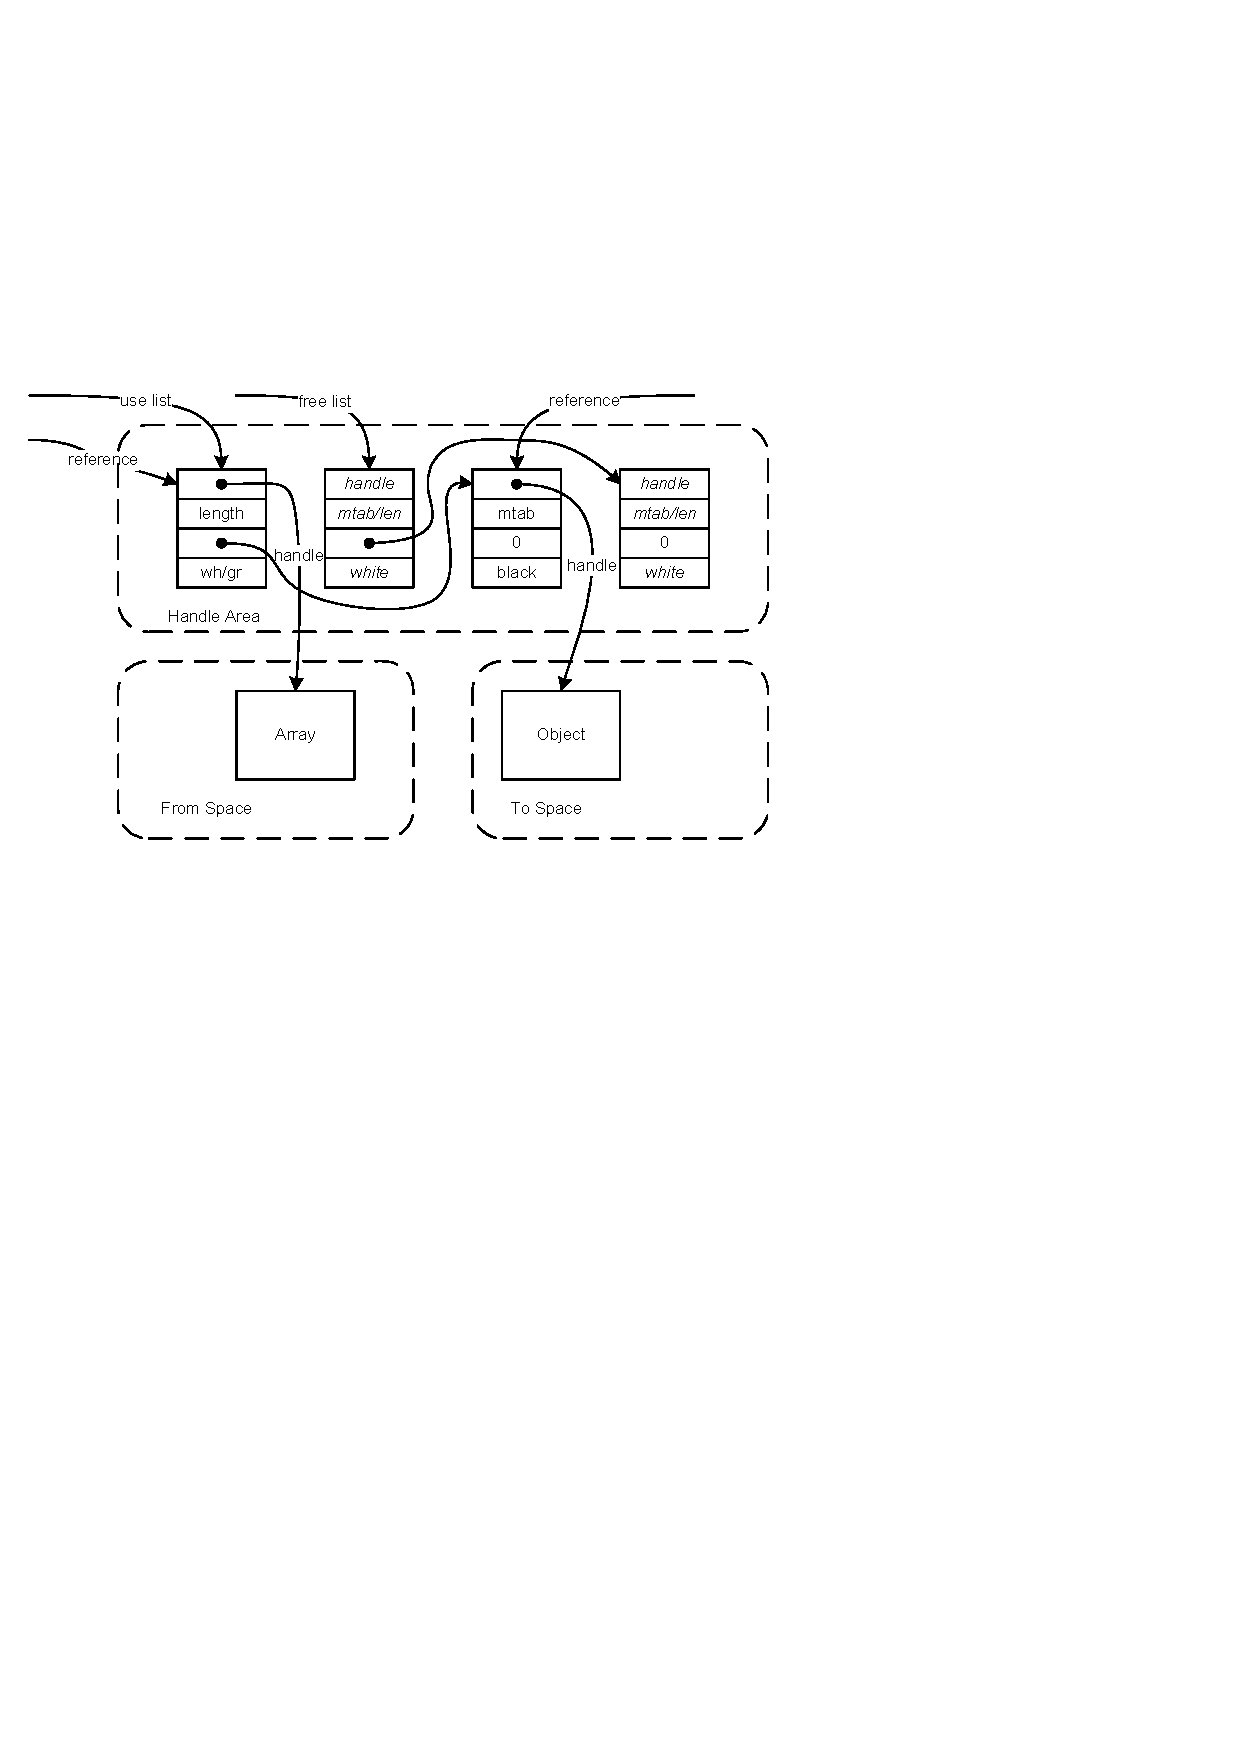
\includegraphics{jvm/handles}
  \caption{Heap layout with the handle area}\label{fig:handles}
\end{figure*}


\section{Implementation}

Our collector is an incremental collector with a
snapshot-at-the-beginning write barrier \cite{gc:yuasa90}. The GC is
based on the copy collector by Cheney \cite{gc:cheney70} and the
incremental version by Baker \cite{gc:baker78}. To avoid the
expensive read barrier in Baker's collector we perform all object
copies concurrently by the collector. Therefore we call it the
\emph{concurrent-copy} collector. We have implemented the
concurrent-copy GC on the Java processor JOP \cite{jop:thesis,
jop:jnl:jsa2007}. The whole collector, the \code{new} operation, and
the write barriers are implemented in Java (with the help of two
native functions for direct memory access). Only the copy operation
is optimized by a faster microcode implementation. Although we show
the implementation on a Java processor, the GC is not JOP specific
and can also be implemented on a conventional processor.

\subsection{Heap Layout}

Figure~\ref{fig:handles} shows a symbolic representation of the heap
layout with the handle area and two semi-spaces, \emph{fromspace} and
\emph{tospace}. Not shown in this figure is the memory region for
runtime constants, such as class information or string constants.
This memory region, although logically part of the heap, is neither
scanned, nor copied by the GC. This constant area contains its own
handles and all references into this area are ignored by the GC.

To simplify object move by the collector, all objects are accessed
with one indirection, called the handle. The handle also contains
auxiliary object data structures, such as a pointer to the method
table or the array length. Instead of Baker's read barrier we have an
additional mark stack which is a threaded list within the handle
structure. An additional field (as shown in Figure~\ref{fig:handles})
in the handle structure is used for a free list and a use list of
handles.

The indirection through a handle, although a very light-weight read
barrier, is usually still considered as a high overhead. Metronome
\cite{gc:bacon03} uses a forwarding pointer as part of the object and
performs forwarding \emph{eagerly}. Once the pointer is forwarded,
subsequent uses of the reference can be performed on the direct
pointer until a GC preemption point. This optimization is performed
by the compiler.

We use a hardware based optimization for this indirection
\cite{jop:oohw:jtres2007}. The indirection is unconditionally
performed in the memory access unit. Furthermore, null pointer checks
and array bounds checks are done in parallel to this indirection.

There are two additional benefits from an explicit handle area instead of a
forwarding pointer: (a) access to the method table or array size needs no
indirection, and (b) the forwarding pointer and the auxiliary data
structures do not need to be copied by the GC.

The fixed handle area is not subject to fragmentation as all handles
have the same size and are recycled at a sweep phase with a simple
free list. However, the reserved space has to be sized (or the GC
period adapted) for the maximum number of objects that are live or
are floating garbage.


\subsection{The Collector}

The collector is scheduled periodically at the lowest priority and
within each period it performs the following steps:
\begin{description}
    \item[Flip] An atomic flip exchanges the roles of tospace and
    fromspace.
    \item[Mark roots] All static references are pushed onto the mark
    stack. Only a single push operation needs to be atomic. As the
    thread stacks are empty we do not need an atomic scan of thread
    stacks.
    \item[Mark and copy] An object is popped from the mark stack,
    all referenced objects, which are still white, are pushed on the
    mark stack, the object is copied to tospace and the handle
    pointer is updated.
    \item[Sweep handles] All handles in the use list are checked if
    they still point into tospace (black objects) or can be added to
    the handle free list.
    \item[Clear fromspace] At the end of the collector work the
    fromspace that contains only white objects is initialized with
    zero. Objects allocated in that space (after the next flip) are
    already initialized and allocation can be performed in constant
    time.
\end{description}
%
The longest atomic operation is the copy of an object or array.  To
reduce blocking time, we plan to implement an array\footnote{Since
objects are typically small, this optimization is likely to pay off
only for arrays.} copy and access hardware module within JOP. The
hardware can perform copies in an interruptible fashion, and records
the copy position on an interrupt. On an array access the hardware
knows whether the access should go to the already copied part in the
tospace or in the not yet copied part in the fromspace. It has to be
noted that splitting larger arrays into smaller chunks, as done in
Metronome~\cite{gc:bacon03} and in the GC for the
JamaicaVM~~\cite{gc:siebert:phd}, is a software option to reduce the
blocking time.

The collector has two modes of operation: one for the initialization
phase and one for the mission phase. At the initialization phase it
operates in a stop-the-world fashion and gets invoked when a memory
request cannot be satisfied. In this mode the collector scans the
stack of the single thread conservatively. It has to be noted that
each reference points into the handle area and not to an arbitrary
position in the heap. This information is considered by the GC to
distinguish pointers from primitives. Therefore the chance to keep an
object artificially alive is low.

As part of the mission start one stop-the-world cycle is performed to
clean up the heap from garbage generated at initialization. From that
point on the GC runs in concurrent mode in its own thread and omits
scanning of the thread stacks.

\subsubsection{Implementation Code Snippets}

This sections shows the important code fragments of the
implementation. As can be seen, the implementation is quite short.

\paragraph{Flip} involves manipulation of a few pointers and changes
the meaning of black (\code{toSpace}) and white.
%
\begin{lstlisting}
    synchronized (mutex) {
        useA = !useA;
        if (useA) {
            copyPtr = heapStartA;
            fromSpace = heapStartB;
            toSpace = heapStartA;
        } else {
            copyPtr = heapStartB;
            fromSpace = heapStartA;
            toSpace = heapStartB;
        }
        allocPtr = copyPtr+semi_size;
    }
\end{lstlisting}


\paragraph{Root Marking} When the GC runs in concurrent mode only
the static reference fields form the root set and are scanned. The
stop-the-world mode of the GC also scans all stacks from all
threads.
%
\begin{lstlisting}
    int addr = Native.rdMem(addrStaticRefs);
    int cnt = Native.rdMem(addrStaticRefs+1);
    for (i=0; i<cnt; ++i) {
        push(Native.rdMem(addr+i));
    }
\end{lstlisting}

\paragraph{Push} All gray objects are pushed on a gray stack. The
gray stack is a list threaded within the handle structure.
%
\begin{lstlisting}
    if (Native.rdMem(ref+OFF_GREY)!=0) {
        return;
    }
    if (Native.rdMem(ref+OFF_GREY)==0) {
        // pointer to former gray list head
        Native.wrMem(grayList, ref+OFF_GREY);
        grayList = ref;
    }
\end{lstlisting}

\paragraph{Mark and Copy} The following code snippet shows the
central GC loop.
%
\begin{lstlisting}
    for (;;) {

        // pop one object from the gray list
        synchronized (mutex) {
            ref = grayList;
            if (ref==GREY_END) {
                break;
            }
            grayList = Native.rdMem(ref+OFF_GREY);
            // mark as not in list
            Native.wrMem(0, ref+OFF_GREY);
        }

        // push all childs
        // get pointer to object
        int addr = Native.rdMem(ref);
        int flags = Native.rdMem(ref+OFF_TYPE);
        if (flags==IS_REFARR) {
            // is an array of references
            int size = Native.rdMem(ref+OFF_MTAB_ALEN);
            for (i=0; i<size; ++i) {
                push(Native.rdMem(addr+i));
            }
        } else if (flags==IS_OBJ){
            // its a plain object
            // get pointer to method table
            flags = Native.rdMem(ref+OFF_MTAB_ALEN);
            // get real flags
            flags = Native.rdMem(flags+MTAB2GC_INFO);
            for (i=0; flags!=0; ++i) {
                if ((flags&1)!=0) {
                    push(Native.rdMem(addr+i));
                }
                flags >>>= 1;
            }
        }

        // now copy it - color it BLACK
        int size = Native.rdMem(ref+OFF_SIZE);
        synchronized (mutex) {
            // update object pointer to the new location
            Native.wrMem(copyPtr, ref+OFF_PTR);
            // set it BLACK
            Native.wrMem(toSpace, ref+OFF_SPACE);
            // copy it
            for (i=0; i<size; ++i) {
                Native.wrMem(Native.rdMem(addr+i), copyPtr+i);
            }
            copyPtr += size;
        }
    }
\end{lstlisting}

\paragraph{Sweep Handles} At the end of the mark and copy phase the
handle area is swept to find all unused handles (the one that still
point into \code{fromSpace}) and add them to the free list.
%
\begin{lstlisting}
    synchronized (mutex) {
        ref = useList;      // get start of the list
        useList = 0;        // new uselist starts empty
    }

    while (ref!=0) {

        int next = Native.rdMem(ref+OFF_NEXT);
        // a BLACK one
        if (Native.rdMem(ref+OFF_SPACE)==toSpace) {
            // add to used list
            synchronized (mutex) {
                Native.wrMem(useList, ref+OFF_NEXT);
                useList = ref;
            }
        // a WHITE one
        } else {
            // add to free list
            synchronized (mutex) {
                Native.wrMem(freeList, ref+OFF_NEXT);
                freeList = ref;
                Native.wrMem(0, ref+OFF_PTR);
            }
        }
        ref = next;
    }
\end{lstlisting}

\paragraph{Clear Fromspace} The last step of the GC clears the
fromspace to provide a constant time allocation after the next flip.
%
\begin{lstlisting}
        for (int i=fromSpace; i<fromSpace+semi_size; ++i) {
            Native.wrMem(0, i);
        }
\end{lstlisting}

\subsection{The Mutator}

The coordination between the mutator and the collector is performed
within the \code{new} and \code{newarray} bytecodes and within write
barriers for JVM bytecodes \code{putfield} and \code{putstatic} for
reference fields, and bytecode \code{aastore}.

\subsubsection{Allocation}

Objects are allocated black (in tospace). In non real-time
collectors it is more common to allocate objects white. It is argued
\cite{gc:dijkstra78} that objects die young and the chances are high
that the GC never needs to touch them. However, in the worst case no
object that is created and becomes garbage during the GC cycle can
be reclaimed. Those floating garbage will be reclaimed in the next
GC cycle. Therefore, we do not benefit from the white allocation
optimization in a real-time GC. Allocating a new object black has
the benefit that those objects do not need to be copied. The same
argument applies to the chosen write barrier. The following code
shows our simple implementation of bytecode \code{new}:

\begin{samepage}
\begin{lstlisting}
synchronized (mutex) {
    // we allocate from the upper part
    allocPtr -= size;
    ref = getHandle(size);
    // mark as object
    Native.wrMem(IS_OBJ, ref+OFF_TYPE);
    // pointer to method table in the handle
    Native.wrMem(cons+CLASS_HEADR, ref+OFF_MTAB_ALEN);
}
\end{lstlisting}
\end{samepage}

As the old fromspace is cleared by the GC we do not need to
initialize the new object and perform \code{new} in constant time.
The methods \code{Native.rdMem()} and \code{Native.wrMem()} provide
direct access to the main memory. Only those two native methods are
necessary for an implementation of a GC in pure Java.

\subsubsection{Write Barriers}

For a concurrent (incremental) GC some coordination between the
collector and the mutator are necessary. The usual solution is a
write barrier in the mutator to not foil the collector. According to
\cite{gc:wils94} GC concurrent algorithms can be categorized into:

\begin{description}
    \item[Snapshot-at-beginning] Keep the object graph as it was at
    the the GC start
    \begin{itemize}
        \item Save to-be-overwritten pointer
        \item More conservative -- not an issue for RTs as worst case
        counts
        \item Allocate black
        \item New objects (e.g.\ new stack frames) do not need a
        write barrier
        \item Optimization: with atomic root scan of the thread
        stacks no write barrier is necessary for locals and the JVM
        stack
    \end{itemize}
    \item[Incremental update] \emph{Help} the GC by doing some collection
    work in the mutator
    \begin{itemize}
        \item Preserve strong tri-color invariant (no pointer from
        black to white objects)
        \item On black to white shade the white object (shade the
        black is unusual)
        \item Allocate black (in contrast to \cite{gc:dijkstra78})
        \item Needs write barriers for locals and manipulation on
        the stack
        \item Less conservative than snapshot-at-beginning
    \end{itemize}
\end{description}

The usual choice is snapshot-at-beginning with atomic root scan of
all thread stacks to avoid write barriers on locals. Assume the
following assignment of a reference:
\begin{lstlisting}
    o.r = ref;
\end{lstlisting}
There are three references involved that can be manipulated:
\begin{itemize}
    \item The old value of \code{o.r}
    \item The new value \code{ref}
    \item The object \code{o}
\end{itemize}
The three possible write barriers are:
\begin{enumerate}
    \item
Snapshot-at-beginning/weak tri-color invariant:
\begin{lstlisting}
    if (white(o.r)) markGrey(o.r);
    o.r = ref;
\end{lstlisting}
    \item
Incremental/strong tri-color invariant with push forward
\begin{lstlisting}
    if (black(o) && white(ref)) markGrey(ref);
    o.r = ref;
\end{lstlisting}
This barrier can be optimized to only check if \code{ref} is white.

    \item
Incremental/strong tri-color invariant with push back
\begin{lstlisting}
    if (black(o) && white(ref)) markGrey(o);
    o.r = ref;
\end{lstlisting}

\end{enumerate}

We have no stack roots when the collector runs. Therefore we could
use the incremental write barrier for object fields only. However,
for the worst case all floating garbage will not be found by the GC
in the current cycle. Therefore, we use the snapshot-at-begin write
barrier in our implementation.



A snapshot-at-begin write barrier synchronizes the mutator with the
collector on a reference store into a static field, an object field,
or an array. The \emph{to be overwritten} field is pushed on the
mark stack when it points to a white object. The following code
shows the implementation of \code{putfield} for reference fields:

\begin{lstlisting}
private static void f_putfield_ref(int ref, int val,
                                    int index) {

    if (ref==0) {
        throw new NullPointerException();
    }
    synchronized (GC.mutex) {
        // handle indirection
        ref = Native.rdMem(ref);
        // snapshot-at-beginning barrier
        int oldVal = Native.rdMem(ref+index);
        if (oldVal!=0 &&
            Native.rdMem(oldVal+GC.OFF_SPACE)!=GC.toSpace) {

            GC.push(oldVal);
        }

        Native.wrMem(val, ref+index);
    }
}
\end{lstlisting}

The shown code is part of a special class (\code{com.jopdesign.sys.JVM})
where Java bytecodes that are not directly implemented by JOP can be
implemented in Java \cite{jop:thesis}. All \code{putfield} bytecodes are
replaced by quick variants on class linking. During this step also
\code{putfield} instructions for references and double-word length fields
(\code{double} and \code{long}) are replaced by special
bytecodes. Therefore, the code shows the special bytecode
\code{putfield\_ref}.



\section{Evaluation}

To evaluate our proposed real-time GC we execute a simple test
application on JOP and measure heap usage and the release time
jitter of high priority threads. The test setup consists of JOP
implemented in an Altera Cyclone FPGA clocked at 100~MHz. The main
memory is a 1~MB SRAM with an access time of two clock cycles. JOP
is configured with a 4~KB method cache (a special form of
instruction cache) and a 128 entry stack cache. No additional data
cache is used.

\subsection{Scheduling Experiments}

In this section we test an implementation of the concurrent-copy
garbage collector on JOP. The tests are intended to get some
confidence that the formulas for the collector periods are correct.
Furthermore we visualize the actual heap usage of a running system.

The examples are synthetic benchmarks that emulate worst-case
execution time (WCET) by executing a busy loop after allocation of
the data. The WCET of the collector was measured to be 10.4~ms when
executing it with scheduling disabled during one collection cycle for
example 1 and 11.2~ms for example 2. We use 11~ms and 12~ms
respectively as the WCET of the collector for the following
examples\footnote{It has to be noted that measuring execution time is
not a safe method to estimate WCET values.}.


Listing~\ref{lst:excode} shows our worker thread with the busy loop.
The data is allocated at the start of the period and freed after the
simulated execution. \code{waitForNextPeriod} blocks until the next
release time for the periodic thread.

\begin{lstlisting}[float, caption={Example periodic thread with a busy loop},
label=lst:excode]
    public void run() {

        for (;;) {
            int[] n = new int[cnt];
            // simulate work load
            busy(wcet);
            n = null;
            waitForNextPeriod();
        }
    }

    final static int MIN_US = 10;

    static void busy(int us) {

        int t1, t2, t3;
        int cnt;

        cnt = 0;
        // get the current time in us
        t1 = Native.rd(Const.IO_US_CNT);

        for (;;) {
            t2 = Native.rd(Const.IO_US_CNT);
            t3 = t2-t1;
            t1 = t2;
            if (t3<MIN_US) {
                cnt += t3;
            }
            if (cnt>=us) {
                return;
            }
        }
    }
\end{lstlisting}

For the busy loop to simulate \emph{real} execution time, and not
elapsed time, the constant \code{MIN\_US} has to be less than the
time for two context switches, but larger than the execution time of
one iteration of the busy loop. In this case only cycles executed by
the busy loop are counted for the execution time and interruption
due to a higher priority thread is not part of the execution time
measurement.

In our example we use a concurrent-copy collector with a heap size
(for both semi-spaces) of 100~KB. At startup the JVM allocates about
3.5~KB data. We incorporate\footnote{We have not yet implemented the
suggested handling of static data to be moved to \emph{immortal}
memory at mission start in our prototype.} these 3.5~KB as static
live data $L_s$.



\subsubsection{Independent Threads}

The first example consists of two threads with the properties listed
in Table~\ref{fig:ex1}. $T_i$ is the period, $C_i$ the WCET, and
$a_i$ the maximum amount of memory allocated each period. Note that
the period for the collector thread is also listed in the table
although it is a result of the worker thread properties and the heap
size.

\begin{table}[tb]
\begin{center}
\begin{tabular}{lrrr}
    \toprule
    & \multicolumn{1}{c}{$T_i$} & \multicolumn{1}{c}{$C_i$} & \multicolumn{1}{c}{$a_i$} \\
    \midrule
    $\tau_1$ & 5 ms & 1 ms & 1 KB \\
    $\tau_2$ & 10 ms & 3 ms & 3 KB \\
    $\tau_{GC}$ & 77 ms & 11 ms & \\
    \bottomrule
\end{tabular}
    \caption{Thread properties for experiment 1}
\label{fig:ex1}
\end{center}
\end{table}

With the periods $T_i$ and the memory consumption $a_i$ for the two
worker threads we calculate the maximum period $T_{GC}$ for the
collector thread $\tau_{GC}$ by using Theorem~\ref{sch:theorem}
\begin{align*}
    T_{GC} & \le \frac{H_{CC}-2\left(L_s+\sum_{i=1}^{n} a_i\right)-2\sum_{i=1}^{n} a_i}
        {2\sum_{i=1}^{n} \frac{a_i}{Ti}} \\
           & \le \frac{100-2(3.5+4)-2\cdot4}
           {2\left(\frac{1}{5}+\frac{3}{10}\right)}\mbox{ms}\\
           & \le 77\mbox{ms}
\end{align*}

The priorities are assigned rate-monotonic \cite{321743} and we
perform a quick schedulability check with the periods $T_i$ and the
WCETs $C_i$ by calculation of the processor utilization $U$ for all
three threads
\begin{align*}
    U & = \sum_{i=1}^{3}\left(\frac{C_i}{T_i}\right)\\
      & = \frac{1}{5} + \frac{3}{10} + \frac{11}{77}\\
      & = 0.643
\end{align*}
which is less than the maximum utilization for three tasks
\begin{align*}
    U_{max} & = m*(2^{\frac{1}{m}}-1)\\
      & = 3*(2^{\frac{1}{3}}-1)\\
      & \approx 0.78
\end{align*}

In Figure~\ref{fig:ex1:mem} the memory trace for this system is
shown.
\begin{figure}
\begin{center}
    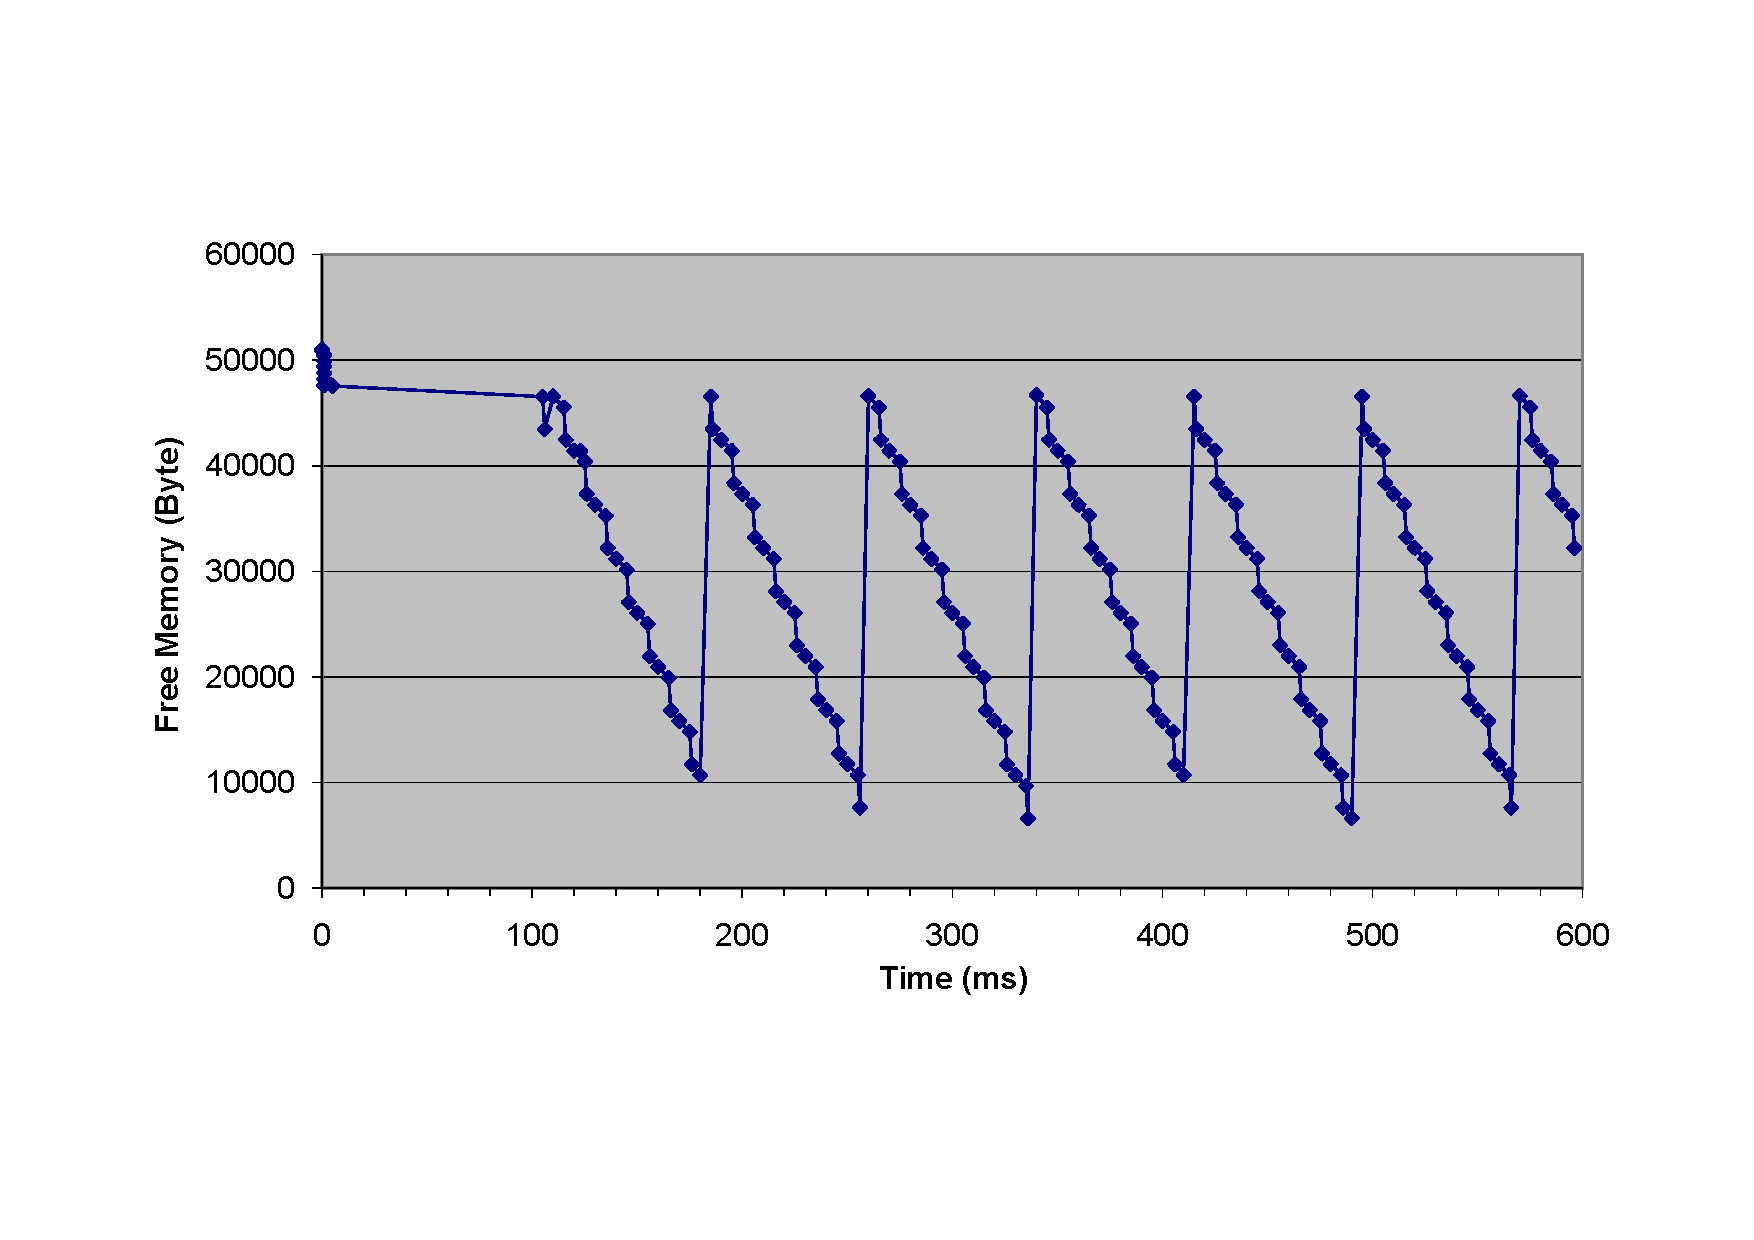
\includegraphics[width=\excelwidth]{jvm/gc_ex1}
    \caption{Free memory in experiment 1}
\label{fig:ex1:mem}
\end{center}
\end{figure}
The graph shows the free memory in one semi-space (the to-space,
which is 50~KB) during the execution of the application. The
individual points are recorded with time-stamps at the end of each
allocation request.

In the first milliseconds we see allocation requests that are part
of the JVM startup (most of it is static data). The change to the
mission phase is delayed 100~ms and the first allocation from a
periodic thread is at 105~ms. The collector thread also starts at
the same time and the first semi-space flip can be seen at 110~ms
(after one allocation from each worker thread). We see the 77~ms
period of the collector in the jumps in the free memory graph after
the flip. The different memory requests of two times 1~KB from
thread $\tau_1$ and one time 3~KB from thread $\tau_2$ can be seen
every 10~ms.

In this example the heap is used until it is almost full, but we run
never out of memory and no thread misses a deadline. From the
regular allocation pattern we also see that this collector runs
concurrently. With a stop-the-world collector we would notice gaps
of 10~ms (the measured execution time of the collector) in the
graph.

\subsubsection{Producer/Consumer Threads}

For the second experiment we split our thread $\tau_1$ to a producer
thread $\tau_1$ and a consumer thread $\tau_3$ with a period of
30~ms. We assume after the split that the producer's WCET is halved
to 500~us. The consumer thread is assumed to be more efficient when
working on lager blocks of data than in the former example
($C_3$=2~ms instead of 6*500~$\mu$s). The rest of the setting
remains the same (the worker thread $\tau_2$). Table~\ref{fig:ex2}
shows the thread properties for the second experiment.

\begin{table}[tb]
\begin{center}
\begin{tabular}{lrrr}
    \toprule
    & \multicolumn{1}{c}{$T_i$} & \multicolumn{1}{c}{$C_i$} &\multicolumn{1}{c}{$a_i$} \\
    \midrule
    $\tau_1$ & 5 ms & 0.5 ms & 1 KB \\
    $\tau_2$ & 10 ms & 3 ms & 3 KB \\
    $\tau_3$ & 30 ms & 2 ms & \\
    $\tau_{GC}$ & 55 ms & 12 ms & \\
    \bottomrule
\end{tabular}
    \caption{Thread properties for experiment 2}
\label{fig:ex2}
\end{center}
\end{table}

As explained in Section~\ref{sec:prod:cons} we calculate the
lifetime factor $l_1$ for memory allocated by the producer $\tau_1$
with the corresponding consumer $\tau_3$ with period $T_3$.
\begin{equation*}
    l_1 = 2\left\lceil\frac{T_3}{T_1}\right\rceil
        = 2\left\lceil\frac{30}{5}\right\rceil
        = 12
\end{equation*}
%
The maximum collector period $T_{GC}$ is
\begin{align*}
    T_{GC} & \le \frac{H_{CC}-2\left(L_s+\sum_{i=1}^{n} a_i l_i\right)-2\sum_{i=1}^{n} a_i}
        {2\sum_{i=1}^{n} \frac{a_i}{Ti}} \\
           & \le \frac{100-2(3.5+1\cdot12+3+0)-2\cdot4}
           {2\left(\frac{1}{5}+\frac{3}{10}+\frac{0}{30}\right)}\mbox{ms}\\
           & \le 55\mbox{ms}
\end{align*}
We check the maximum processor utilization:
\begin{align*}
    U & = \sum_{i=1}^{4}\left(\frac{C_i}{T_i}\right)\\
      & = \frac{0.5}{5} + \frac{3}{10} + \frac{2}{30} + \frac{12}{55}\\
      & = 0.685 \le 4*(2^{\frac{1}{4}}-1) \approx 0.76
\end{align*}

In Figure~\ref{fig:ex2:mem} the memory trace for the system with one
producer, one consumer, and one independent thread is shown.
\begin{figure}
\begin{center}
    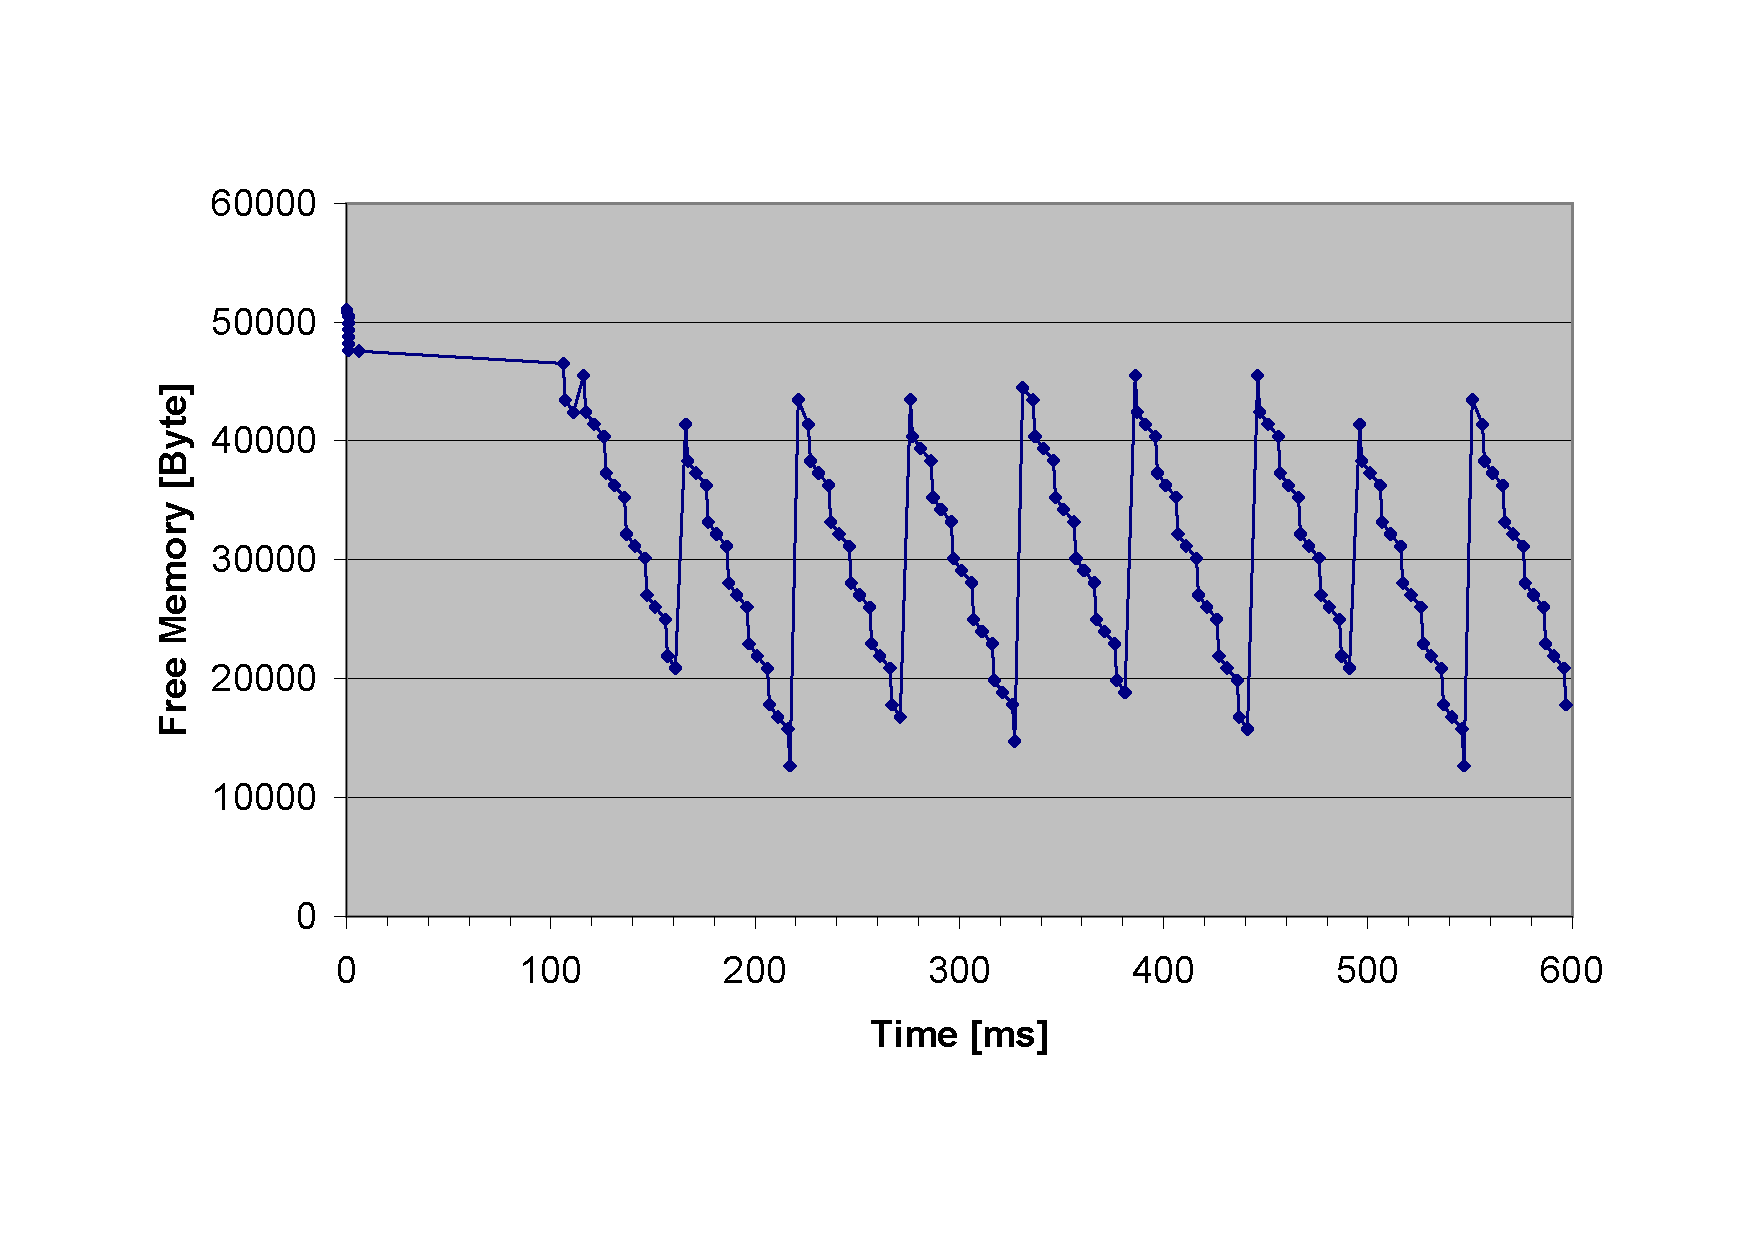
\includegraphics[width=\excelwidth]{jvm/gc_ex2}
    \caption{Free memory in experiment 2}
\label{fig:ex2:mem}
\end{center}
\end{figure}
%
Again, we see the 100~ms delayed mission start after the startup and
initialization phase, in this example at about 106~ms. Similar to
the former example the first collector cycle performs the flip a few
milliseconds after the mission start. We see the shorter collection
period of 55~ms. The allocation pattern (two times 1~KB and one time
3~KB per 10~ms) is the same as in the former example as the threads
that allocate the memory are still the same.

We have also run this experiment for a longer time than shown in
Figure~\ref{fig:ex2:mem} to see if we find a point in the execution
trace where the remaining free memory is less than the value at
217~ms. The pattern repeats and the observed value at 217~ms is the
minimum.




\subsection{Measuring Release Jitter}

Our main concern on garbage collection in real-time systems is the
blocking time introduced  by the GC due to atomic code sections.
This blocking time will be seen as release time jitter on the
real-time threads. Therefore we want to measure this jitter.

\begin{lstlisting}[float, caption={Measuring release time jitter},
label=lst:measure]

public boolean run() {

    int t = Native.rdMem(Const.IO_US_CNT);
    if (!notFirst) {
        expected = t+period;
        notFirst = true;
    } else {
        int diff = t-expected;
        if (diff>max) max = diff;
        if (diff<min) min = diff;
        expected += period;
    }
    work();

    return true;
}
\end{lstlisting}

Listing~\ref{lst:measure} shows how we measure the jitter. Method
\code{run()} is the main method of the real-time thread and executed
on each periodic release. Within the real-time thread we have no
notion about the start time of the thread. As a solution we measure
the actual time on the first iteration and use this time as first
release time. In each iteration the expected time, stored in the
variable \code{expected}, is incremented by the \code{period}. In
each iteration (except the first one) the actual time is compared
with the expected time and the maximum value of the difference is
recorded.

As noted before, we have no notion about the \emph{correct} release
times. We measure only relative to the first release. When the first
release is delayed (due to some startup code or interference with a
higher priority thread) we have a positive offset in
\code{expected}. On an exact release in a later iteration the time
difference will be negative (in \code{diff}). Therefore, we also
record the minimum value for the difference between the actual time
and the expected time. The maximum measured release jitter is the
difference between \code{max} and \code{min}.

To provide a baseline we measure the release time jitter of a single
real-time thread (plus an endless loop in the \code{main} method as
an idle non-real-time background thread). No GC thread is scheduled.
The code is similar to the code in in Figure~\ref{lst:measure}. A
stop condition is inserted that prints out the minimum and maximum
time differences measured after 1 million iterations.

\begin{table}
    \centering
    \begin{tabular}{rr}
    \toprule
    Period & Jitter \\
    \midrule
    200 $\mu$s & 0 $\mu$s \\
    100 $\mu$s & 0 $\mu$s \\
    50 $\mu$s & 17 $\mu$s \\
    \bottomrule
    \end{tabular}
    \caption{Release jitter for a single thread}
    \label{tab:single}
\end{table}

Table~\ref{tab:single} shows the measured jitter for different
thread periods. We observed no jitter for periods of 100~$\mu$s and
longer. At a period of 50~$\mu$s the scheduler introduces a
considerable amount of jitter. From this measurement we conclude
that 100~$\mu$s is the practical shortest period we can handle with
our system. We will use this period for the high-priority real-time
thread in the following measurement with an enabled GC.

\subsection{Measurements}

The test application consisting of three real-time threads
($\tau_{hf}$, $\tau_{p}$, and $\tau_{c}$), one logging thread
$\tau_{log}$, and the GC thread $\tau_{gc}$. All three real-time
threads measure the difference between the expected release time and
the actual release time (as shown in Figure~\ref{lst:measure}). The
minimum and maximum values are recorded and regularly printed to the
console by the logging thread $\tau_{log}$. Table~\ref{tab:exp}
shows the release parameters for the five threads. Priority is
assigned deadline monotonic. Note that the GC thread has a shorter
period than the logger thread, but a longer deadline. For our
approach to work correctly the GC thread \emph{must} have the lowest
priority. Therefore all other threads with a longer period than the
GC thread must be assigned a shorter deadline.

\begin{table}
    \centering
    \begin{tabular}{lrrr}
    \toprule
    Thread & Period & Deadline & Priority \\
    \midrule
    $\tau_{hf}$ & 100 $\mu$s & 100 $\mu$s & 5 \\
    $\tau_{p}$ &  1 ms & 1 ms & 4 \\
    $\tau_{c}$ & 10 ms & 10 ms & 3 \\
    $\tau_{log}$ & 1000 ms & 100 ms & 2 \\
    $\tau_{gc}$ & 200 ms & 200 ms & 1 \\
    \bottomrule
    \end{tabular}
    \caption{Thread properties of the test program}
    \label{tab:exp}
\end{table}

Thread $\tau_{hf}$ represents a high-frequency thread without
dynamic memory allocation. This thread should observe minimal
disturbance by the GC thread.

The threads $\tau_{p}$ and $\tau_{c}$ represent a producer/consumer
pair that uses dynamically allocated memory for communication. The
producer appends the data at a frequency of 1~kHz to a simple list.
The consumer thread runs at 100~Hz and processes all currently
available data in the list and removes them from the list. The
consumer will process between 9 and 11 elements (depending on the
execution time of the consumer and the thread phasing).

It has to be noted that this simple and common communication pattern
cannot be implemented with the scoped memory model of the RTSJ.
First, to use a scope for communication, we have to keep the scope
alive with a \emph{wedge} thread \cite{conf/isorc/PizloFHV04} when
data is added by the producer. We would need to notify this wedge
thread by the consumer when all data is consumed. However, there is
no single instant available where we can \emph{guarantee} that the
list is empty. A possible solution for this problem is described in
\cite{conf/isorc/PizloFHV04} as \emph{handoff} pattern. The pattern
is similar to double buffering, but with an explicit copy of the
data. The elegance of a simple list as buffer queue between the
producer and the consumer is lost.

Thread $\tau_{log}$ is not part of the real-time systems simulated
application code. Its purpose is to print the minimum and maximum
differences between the measured and expected release times (see
former section) of threads $\tau_{hf}$ and $\tau_{p}$ to the console
periodically.

Thread $\tau_{gc}$ is a standard periodic real-time thread executing
the GC logic. The GC thread period was chosen quite short in that
example. A period in the range of seconds would be enough for the
memory allocation by $\tau_{p}$. However, to stress the interference
between the GC thread and the application threads we artificially
shortened the period.

\begin{table}
    \centering
    \begin{tabular}{lr}
    \toprule
    Threads & Jitter \\
    \midrule
    $\tau_{hf}$ & 0 $\mu$s \\
    $\tau_{hf}$, $\tau_{log}$ & 7 $\mu$s \\
    $\tau_{hf}$, $\tau_{log}$,$\tau_{p}$,$\tau_{c}$ & 14 $\mu$s \\
    $\tau_{hf}$, $\tau_{log}$,$\tau_{p}$,$\tau_{c}$,$\tau_{gc}$ & 54 $\mu$s \\
    \bottomrule
    \end{tabular}
    \caption{Jitter measured on a 100~MHz processor for the high priority thread in different configurations}
    \label{tab:jitter}
\end{table}
As a first experiment we run only $\tau_{hf}$ and the logging thread
$\tau_{log}$ to measure jitter introduced by the scheduler. The
maximum jitter observed for $\tau_{hf}$ is 7 $\mu$s -- the blocking
time of the scheduler.

In the second experiment we run all threads except the GC thread.
For the first 4 seconds we measure a maximum jitter of 14~$\mu$s for
thread $\tau_{hf}$. After those 4 seconds the heap is full and GC is
necessary. In that case the GC behaves in a stop-the-world fashion.
When a new object request cannot be fulfilled the GC logic is
executed in the context of the allocating thread. As the bytecode
\code{new} is itself in an atomic region the application is blocked
until the GC finishes. Furthermore, the GC performs a conservative
scan of all thread stacks. We measure a release delay of 63~ms for
all threads due to the blocking during the full collection cycle.
From that measurement we can conclude for the sample application and
the available main memory: (a) the measured maximum period of the GC
thread is in the range of 4 seconds; (b) the estimated execution
time for one GC cycle is 63~ms. It has to be noted that measurement
is not a substitution for static timing analysis. Providing WCET
estimates for a GC cycle is a challenge for future work.

In our final experiment we enabled all threads. The GC is scheduled
periodically at 200~ms as the lowest priority thread -- the scenario
we argue for. The GC logic is set into the concurrent mode on mission
start. In this mode the thread stacks are not scanned for roots.
Furthermore when an allocation request cannot be fulfilled the
application is stopped. This radical stop is intended for testing. In
a more tolerant implementation either an out-of-memory exception can
be thrown or the requesting thread has to be blocked, its thread
stack scanned and released when the GC has finished its cycle.

We ran the experiment for several hours and recorded the maximum
release jitter of the real-time threads. For this test we used
slightly different periods (prime numbers) to avoid the regular
phasing of the threads. The harmonic relation of the original
periods can lead to too optimistic measurements. The applications
never ran out of memory. The maximum jitter observed for the high
priority task $\tau_{hf}$ was 54~$\mu$s. The maximum jitter for task
$\tau_{p}$ was 108~$\mu$s. This higher value on $\tau_{p}$ is
expected as the execution interferes with the execution of the
higher priority task $\tau_{hf}$.

\subsection{Discussion}


With our measurements we have shown that quite short blocking times
are achievable. Scheduling introduces a blocking time of about
7--14~$\mu$s and the GC adds another 40~$\mu$s resulting in a
maximum jitter of the highest priority thread of 54~$\mu$s. In our
first implementation we performed the object copy in pure Java,
resulting in blocking times around 200~$\mu$s. To speedup the copy
we moved this function to microcode. However, the microcoded
\emph{memcpy} still needs 18 cycles per 32-bit word copy. Direct
support in hardware can lead to a copy time of 4--5 clock cycles per
word.

The maximum blocking time of 54~$\mu$s on a 100 MHz processor is less than
blocking times reported for other solutions.

Blocking time for Metronome (called pause times in the papers) is
reported to be 6~ms \cite{gc:jtres:metronome} on a 500~MHz PowerPC
at 50\% CPU utilization. Those large blocking times are due to the
scheduling of the GC at the highest priority with a polling based
yield within the GC thread. A fairer comparison is against the
\emph{jitter} of the pause time. In \cite{gc:bacon05} the variation
of the pause time is given between 500~$\mu$s and 2.4~ms on a 1~Ghz
machine. It should be noted that Metronome is a GC intended for
mixed real-time systems whereas we aim only for hard real-time
systems.

Robertz performed a similar measurement as we did for his thesis
\cite{gc:robertz:thesis} with a time-triggered GC on a 350~MHz
PowerPC. He measured a maximum jitter of 20~$\mu$s ($\pm10$~$\mu$s)
for a high priority task with a period of 500~$\mu$s.

It has to be noted that our experiment is a small one and we need
more advanced real-time applications for the evaluation of real-time
GC. The problem is that it is hard to find even static based
real-time application benchmarks (at least applications written for
safety critical Java). Running standard benchmarks that measure
average case performance (e.g., SPEC jvm98) is not an option to
evaluate a real-time collector.

%SUN RTS jitter +- 10us, but heap schedulables 100us
%lund release time jitter 40us - from where do I have this number
%\url{http://www.robot.lth.se/java/} compiler
%read \url{http://www.ulb.ac.be/di/ssd/goossens/RTS05.pdf}

%\subsection{Future Enhancements}

Although we measured a low blocking time in our experiment we think
there is room for improvements. As a first enhancement we will
implement a hardware \emph{memcpy} in the memory unit of JOP to
reduce the blocking time. However, for very large arrays the
resulting blocking time may still be too large. A common solution is
to break up arrays into smaller chunks sometimes called Arraylets
\cite{gc:bacon03}. However, this comes at a more complex array
access with a higher cost.

As we are running our GC on a soft-core Java processor our design
space is larger and we can consider implementing a function unit
that supports incremental copy. This copy unit will be integrated
with the array (field) access unit. On a timer interrupt (for a
scheduling decision) the memory copy will also be interrupted and
the application thread can run. The copy/access unit remembers the
copy position and will redirect the array/field access either to
fromspace or to tospace.

Another option is a full hardware implementation of the GC. The
proposed algorithm is not very complex and should result in a not
too complex hardware. However, this design direction should be
carefully evaluated against a way simpler parallel solution: running
the GC on one CPU of a chip multiprocessor version of JOP.

\section{Analysis}

To integrate GC into the WCET and scheduling analysis we need to
know the worst-case memory consumption including the maximum
lifetime of objects and the WCET of the collector itself.

\subsection{Worst Case Memory Consumption}

Similar to the necessary WCET analysis of the tasks that make up the
real-time system, a worst case memory allocation analysis of the
tasks is necessary. For objects that are not shared between tasks
this analysis can be performed by the same methods known from the
WCET analysis. We have to find the worst-case program path that
allocates the maximum amount of memory.

The analysis of memory consumption by objects that are shared
between tasks for communication is more complex as an inter-task
analysis is necessary.

\subsection{WCET of the Collector}

For the schedulability analysis the WCET of the collector has to be
known. The collector performs following steps\footnote{These steps
can be distinct steps as in the mark-compact collector or
interleaved as in the concurrent-copy collector.}:
\begin{enumerate}
    \item Traverse the live object graph
    \item Copy the live data
    \item Initialize the free memory
\end{enumerate}

The execution time of the first step depends on the maximum amount
of live data and the number of references in each object. The second
step depends on the size of the live objects. The last step depends
on the size of the memory that gets freed during the collection
cycle. For a concurrent-copy collector this time is constant as a
complete semi-space gets initialized to zero. It has to be noted
that this initialization could also be done at the allocation of the
objects (as the \code{LTMemory} from the RTSJ implies). However,
initialization in the collector is more efficient and the necessary
time is easier to predict.

The maximum allocated memory and the type of the allocated objects
determine the control flow (the flow facts) of the collector.
Therefore, this information has to be to incorporate into WCET
analysis of the collector thread.

\section{Summary} \label{sec:gc:summery}

In this chapter we have presented a real-time garbage collector in
order to benefit from a more dynamic programming model for real-time
applications. Our collector is incremental and scheduled as a normal
real-time thread and, according to its deadline, assigned the lowest
priority in the system. The restrictions from the SCJ programming
model and the low priority result in two advantages: (a) avoidance of
stack root scanning and (b) short blocking time of high priority
threads. We have implemented the proposed GC on the Java processor
JOP. At 100~MHz we measured 40~$\mu$s maximum blocking time
introduced by the GC thread.

To guarantee that the applications will not run out of memory, the
period of the collector thread has to be short enough. We provided
the maximum collector periods for a mark-compact collector type and a
concurrent-copy collector. We have also shown how a longer lifetime
due to object sharing between threads can be incorporated into the
collector period analysis.

A critical operation for a concurrent, compacting GC is the atomic
copy of large arrays. We consider extending JOP with a copy unit that
can be interrupted. This unit is integrated with the array access
unit and will redirect the access to either fromspace or tospace
depending on the array index and the value of the copy pointer.

\section{Further Reading}

Garbage collection was first introduced for list processing systems
(LISP) in the 1960s. The first collectors were \emph{stop-the-world}
collectors that are called when a request for a new element can not
be fulfilled. The collector, starting from pointers known as the root
set, scans the whole graph of reachable objects and marks these
objects live. In a second phase the collector \emph{sweeps} the heap
and adds unmarked objects to the free list. On the marked objects,
which are live, the mark is reset in preparation for the next cycle.

However, this simple sweep results in a fragmented heap which is an
issue for objects of different sizes. An extension, called
\emph{mark-compact}, moves the objects to compact the heap instead
of the sweep. During this compaction all references to the moved
objects are updated to point to the new location.


Both collectors need a stack during the marking phase that can grow
in the worst-case up to the number of live objects. Cheney
\cite{gc:cheney70} presents an elegant way how this mark stack can
be avoided. His GC is called \emph{copying-collector} and divides
the heap into two spaces: the \emph{to-space} and the
\emph{from-space}. Objects are moved from one space to the other as
part of the scan of the object graph.

However, all the described collectors are still stop-the-world
collectors. The pause time of up to seconds in large interactive
LISP applications triggered the research on incremental collectors
that distribute collection work more evenly \cite{gc:steele75,
gc:dijkstra78, gc:baker78}. These collectors were sometimes called
\emph{real-time} although they do not fulfill hard real-time
properties that we need today. A good overview of GC techniques can
be found in \cite{gc:jone96} and in the GC survey by Wilson
\cite{gc:wils94}.

\subsection{Related Work}

Baker \cite{gc:baker78} extends Cheneys \cite{gc:cheney70} copying
collector for incremental GC. However, it uses an expensive read
barrier that moves the object to the to-space as part of the mutator
work. Baker proposes the \emph{Treadmill} \cite{gc:baker92} to avoid
copying. However, this collector works only with objects of equal
size and still needs an expensive read barrier.

In \cite{gc:hwgc94} a garbage-collected memory module is suggested to
provide a real-time collector. A worst-case delay time of 1$\mu$s is
claimed without giving the processor speed.

Despite the title \cite{gc:bacon03} is still not a real-time
collector. Non real-time applications are used (SPECjvm98) in the
experiments. They propose a collector with constant utilization to
meet real-time requirements. However, utilization is \emph{not} a
real-time measure per se; it should be schedulability or response
time instead. Pause times are in the range of 12ms.

In \cite{gc:pfeffer04} two collectors based on \cite{gc:dijkstra78}
and \cite{gc:baker92} are implemented on a multithreaded
microcontroller.  Higuera suggests in \cite{gc:higu02} the use of
hardware features from picoJava to speed up RTSJ memory region
protection and garbage collection.

In \cite{780745} the authors provide an upper bound in the GC cycle
time as\footnote{We use our symbols in the equation for easier
comparison to our finding.}
%
\begin{equation}
\nonumber
    T_{GC} \le \frac{\frac{H-L_{max}}{2}-\sum_{i=1}^{n} a_i}{\sum_{i=1}^{n} \frac{a_i}{Ti}}
\end{equation}
%
Although stated that this bound ``is thus not dependent of any
particular GC algorithm", the result applies only for single heap GC
algorithms (e.g.\ mark-compact) and not for a copying collector. A
value for $L_{max}$ is not given in the paper. If we use our value
of $L_{max} =\sum_{i=1}^{n} a_i$ the result is
%
\begin{equation}
\nonumber
    T_{GC} \le \frac{H-3\sum_{i=1}^{n} a_i}{2\sum_{i=1}^{n} \frac{a_i}{Ti}}
\end{equation}
%
This result is the same as in our finding (see
Theorem~\ref{sch:theorem}) for the mark-compact collector. No
analysis is given how objects with longer lifetime and static
objects can be incorporated.


\chapter{Worst-Case Execution Time}
\label{chap:wcet}
    Worst-case execution time (WCET) estimates of tasks are essential
for designing and verifying real-time systems. WCET estimates can be
obtained either by measurement or static analysis. The problem with
using measurements is that the execution times of tasks tend to be
sensitive to their inputs. As a rule, measurement does not guarantee
safe WCET estimates. Instead, static analysis is necessary for hard
real-time systems. Static analysis is usually divided into a number
of different phases:
\begin{description}
    \item[Path analysis] generates the control flow graph (a directed
    graph of basic blocks) of the program and annotates (manual or
    automatic) loops with bounds.
    \item[Low-level analysis] determines the execution time of basic
    blocks obtained by the path analysis. A model of the processor
    and the pipeline provides the execution time for the instruction
    sequence.
    \item[Global low-level analysis] determines the influence of
    hardware features such as caches on program execution time. This
    analysis can use information from the path analysis to provide less
    pessimistic values.
    \item[WCET Calculation] The final WCET is calculated by
        transforming the control flow graph with the timing
        information of basic blocks\footnote{A basic block is a
        sequence of instructions without any jumps or jump
        targets within this sequence.} with the program
        annotations for loops to an integer linear programming
        (ILP) problem. This problem is solved by an ILP solver.
        This approach is also called implicit path enumeration
        (IPET).
\end{description}

For the low-level analysis, a good timing model of the processor is
needed. The main problem for the low-level analysis is the execution
time dependency of instructions in modern processors that are not
designed for real-time systems. JOP is designed to be an easy target
for WCET analysis. The WCET of each bytecode can be predicted in
terms of the number of cycles it requires. There are no timing
dependencies between bytecodes.

WCET analysis has to be done at two levels: at the microcode level
and at the bytecode level. The microcode WCET analysis is performed
only once for a processor configuration and described in the next
section. The result from this microcode analysis is the timing model
of the  processor. The timing model is the input for the WCET
analysis at the bytecode level (i.e.\ the Java application) as
explained in Section~\ref{sec:wcet:app}.

The first WCET analysis tool that targets JOP has been developed by
Rasmus Pedersen \cite{jop:wcet:jtres06}. Benedikt Huber implemented a
new version of the analyzer with support of bytecodes implemented in
Java and a better method cache approximation has
\cite{jop:wcet:model:checking}. The new tool also contains a module
to extract the low-level bytecode timing from the microcode assembler
program (\code{jvm.asm}) automatically.

\section{Microcode WCET Analysis}

Each bytecode is implemented by microcode. We can obtain the WCET of
a single bytecode by performing WCET analysis at the microcode level.
To prove that there are no time dependencies between bytecodes, we
have to show that no processor states are \emph{shared} between
different bytecodes.

\subsection{Microcode Path Analysis}

To obtain the WCET values for the individual bytecodes we perform
the path analysis at the microcode level. First, we have to ensure
that a number of restrictions (from \cite{pusch:maxt:jnl}) of the
code are fulfilled:
%
\begin{itemize}
    \item Programs must not contain unbounded recursion. This property
    is satisfied by the fact that there exists no call instruction in
    microcode.
    \item Function pointers and computed \code{gotos} complicate the
    path analysis and should therefore be avoided. Only simple conditional
    branches are available at the microcode level.
    \item The upper bound of each loop has to be known. This is the only
    point that has to be verified by inspection of the microcode.
\end{itemize}
%
To detect loops in the microcode we have to find all backward
branches (e.g.\ with a negative branch offset)\footnote{The loop
branch can be a forward branch. However, the basic blocks of the
loop contain at least one backward branch. Therefore we can identify
all loops by searching for backward branches only.}. The branch
offsets can be found in a VHDL file (\code{offtbl.vhd}) that is
generated during microcode assembly. In the current implementation
of the JVM there are ten different negative offsets. However, not
each offset represents a loop. Most of these branches are used to
share common code. Three branches are found in the initialization
code of the JVM. They are not part of a bytecode implementation and
can be ignored. The only loop that is found in a regular bytecode is
in the implementation of \code{imul} to perform a fixed delay. The
iteration count for this loop is constant.

A few bytecodes are implemented in Java\footnote{The implementation
can be found in the class \code{com.jopdesign.sys.JVM}.} and can be
analyzed in the same way as application code. The bytecodes
\code{idiv} and \code{irem} contain a constant loop. The bytecode
\code{lookupswitch}\footnote{\codefoot{lookupswitch} is one way of
implementing the Java \codefoot{switch} statement. The other
bytecode, \codefoot{tableswitch}, uses an index in the table of
branch offsets and has therefore a constant execution time.} performs
a linear search through a table of branch offsets. The WCET depends
on the table size that can be found as part of the instruction.

As the microcode sequences are very short, the calculation of the
control flow graph for each bytecode is done manually.

\subsection{Microcode Low-level Analysis}

To calculate the execution time of basic blocks in the microcode, we
need to establish the timing of microcode instructions on JOP. All
microcode instructions except \code{wait} execute in a single cycle,
reducing the low-level analysis to a case of merely counting the
instructions.

The \code{wait} instruction is used to stall the processor and wait
for the memory subsystem to finish a memory transaction. The
execution time of the \code{wait} instruction depends on the memory
system and, if the memory system is predictable, has a known WCET. A
main memory consisting of SRAM chips can provide this predictability
and this solution is therefore advised. The predictable handling of
DMA, which is used for the instruction cache fill, is explained in
Section~\ref{sec:cache}. The \code{wait} instruction is the only way
to stall the processor. Hardware events, such as interrupts (see
Section~\ref{sec:interrupt}), do not stall the processor.

Microcode is stored in on-chip memory with single cycle access. Each
microcode instruction is a single word long and there is no need for
either caching or prefetching at this stage. We can therefore omit
the low-level analysis. No pipeline analysis \cite{EngblomPhD}, with
its possible unbound timing effects, is necessary.

\subsection{Bytecode Independency}

We have seen that all microcode instructions except \code{wait} take
one cycle to execute and are therefore independent of other
instructions. This property directly translates to independency of
bytecode instructions.

The \code{wait} microcode instruction provides a convenient way to
hide memory access time. A memory read or write can be triggered in
microcode and the processor can continue with microcode
instructions. When the data from a memory read is needed, the
processor explicitly waits, with the \code{wait} instruction, until
it becomes available.

For a memory store, this \code{wait} could be deferred until the
memory system is used next (similar to a write buffer). It is
possible to initiate the store in a bytecode such as \code{putfield}
and continue with the execution of the next bytecode, even when the
store has not been completed. In this case, we introduce a
dependency over bytecode boundaries, as the state of the memory
system is \emph{shared}. To avoid these dependencies that are
difficult to analyze, each bytecode that accesses memory waits
(preferably at the end of the microcode sequence) for the completion
of the memory request.

Furthermore, if we would not wait at the end of the store operation
we would have to insert an additional \code{wait} at the start of
every read operation. Since read operations are more frequent than
write operations (15\% vs. 2.5\%, see \cite{jop:thesis}), the
performance gain from the hidden memory store is lost.

\subsection{WCET of Bytecodes}

\label{sec:wcet:bc} The control flow of the individual bytecodes
together with the basic block length (that directly corresponds with
the execution time) and the time for memory access result in the WCET
(and BCET) values of the bytecodes. These values can be found in
Appendix~\ref{appx:bytecode}.

\subsubsection{Basic Bytecodes}

Most bytecode instructions that do not access memory have a constant
execution time. They are executed by either one microcode instruction
or a short sequence of microcode instructions. The execution time in
clock cycles equals the number of microinstructions executed. As the
stack is on-chip, it can be accessed in a single cycle. We do not
need to incorporate the main memory timing into the instruction
timing. Most simple bytecodes execute in a single cycle.
Table~\ref{tab:simple} shows example instructions, their timing, and
their meaning. Access to object, array, and class fields depend on
the timing of the main memory.

\begin{table}
\centering
\begin{tabular}{rlcl}
    \toprule
    Opcode & Instruction & Cycles & Funtion\\
    \midrule
3 & iconst\_0  & 1 & load constant 0 on TOS\\
4 & iconst\_1  & 1 & load constant 1 on TOS\\
16 & bipush & 2 & load a byte constant on TOS\\
17 & sipush & 3 & load a short constant on TOS\\
21 & iload  & 2 & load a local on TOS\\
26 & iload\_0 & 1 & load local 0 on TOS\\
27 & iload\_1 & 1 & load local 1 on TOS\\
54 & istore  & 2 & store the TOS in a local\\
59 & istore\_0 & 1 & store the TOS in local 0\\
60 & istore\_1 & 1 & store the TOS in local 1\\
89 & dup & 1 & duplicate TOS\\
90 & dup\_x1 & 5 & complex stack manipulation\\
96 & iadd & 1 & integer addition\\
153 & ifeq & 4 & conditional branch\\
    \bottomrule
\end{tabular}
    \caption{Execution time of simple bytecodes in cycles}
    \label{tab:simple}
\end{table}


\subsubsection{Object Oriented Bytecodes}

Object oriented instructions, array access, and invoke instructions
access the main memory. Therefore, we have to model the memory access
time. We assume a simple SRAM with a constant access time. Access
time that exceeds a single cycle includes additional wait states
($r_{ws}$ for a memory read and $w_{ws}$ for a memory write). With a
memory with $r_{ws}$ wait states, the execution time for, e.g.,
\code{getfield} is
\begin{equation*}
    t_{\textit{getfield}} = 11 + 2 r_{ws}
\end{equation*}

The memory subsystem performs reads and writes in parallel to the
execution of microcode. Therefore, some access cycles can be hidden.
The following example gives the exact execution time of bytecode
\code{ldc2\_w} in clock cycles:

\begin{equation*}
    t_{ldc2\_w} = 17+\left\{\begin{array}{r@{\quad:\quad}l}
    r_{ws}-2 & r_{ws}>2 \\
    0   & r_{ws}\le2
    \end{array} \right.
    +
    \left\{\begin{array}{r@{\quad:\quad}l}
    r_{ws}-1 & r_{ws}>1 \\
    0   & r_{ws}\le1
    \end{array} \right.
\end{equation*}

Thus, for a memory with two cycles access time ($r_{ws}=1)$, as we
use it for a 100~MHz version of JOP with a 15~ns SRAM, the wait state
is completely hidden by microcode instructions for this bytecode.

Memory access time also determines the cache load time on a miss. For
the current implementation the cache load time is calculated as
follows: the wait state $c_{ws}$ for a single word cache load is:
\begin{equation*}
    c_{ws} =
    \left\{\begin{array}{r@{\quad:\quad}l}
    r_{ws} & r_{ws}>1 \\
    1   & r_{ws}\le1
    \end{array} \right.
\end{equation*}
%
On a method invoke or return, the respective method has to be loaded
into the cache on a cache miss. The load time $l$ is:
\[
    l =
    \left\{\begin{array}{r@{\quad:\quad}l}
    6+(n+1)(1+c_{ws}) & \mbox{cache miss} \\
    4   & \mbox{cache hit}
    \end{array} \right.
\]
where $n$ is the size of the method in number of 32-bit words. For
short methods, the load time of the method on a cache miss, or part
of it, is hidden by microcode execution. As an example, the exact
execution time for the bytecode \code{invokestatic} is:
%
\begin{equation*}
    t = 74+r_{ws}+
    \left\{\begin{array}{r@{\quad:\quad}l}
    r_{ws}-3 & r_{ws}>3 \\
    0   & r_{ws}\le3
    \end{array} \right.
    +
    \left\{\begin{array}{r@{\quad:\quad}l}
    r_{ws}-2 & r_{ws}>2 \\
    4   & r_{ws}\le2
    \end{array} \right.
    +
    \left\{\begin{array}{r@{\quad:\quad}l}
    l-37 & l>37 \\
    0   & l\le37
    \end{array} \right.
\end{equation*}
%

For \code{invokestatic} a cache load time $l$ of up to 37 cycles is
completely hidden. For the example SRAM timing the cache load of
methods up to 36 bytes long is hidden. The WCET analysis tool, as
described in the next section, knows the length of the invoked method
and can therefore calculate the time for the invoke instruction cycle
accurate.

\subsubsection{Bytecodes in Java}

Bytecodes can be implemented in Java on JOP. In this case, a static
method from a JVM internal class gets invoked when such a bytecode is
executed. For the WCET analysis this bytecode is substituted by an
invoke instruction to this method. The influence on the cache (the
bytecode execution results in a method load) can be analyzed in the
same way as for \emph{ordinary} static methods.

%\begin{itemize}
%    \item Java based bytecodes -- handle them as methods
%    \item \code{new} with constant execution time (in our current GC
%    implementation and also possible with scopes)
%\end{itemize}

\subsubsection{Native Methods}

Most of the JVM internal functionality in JOP, such as input, output,
and thread scheduling, is implemented in Java. However, Java and the
JVM do not allow direct access to memory, peripheral devices or
processor registers. For this low-level access to system resources,
we need \emph{native} methods. For a Java processor, the
\emph{native} language is still Java bytecode. We solve this issue by
substituting the native method invocation by a special bytecode
instruction on class loading. Those special bytecodes are implemented
in JOP microcode in the same way as regular bytecodes (see
Section~\ref{sec:microcode}. The execution time of the native methods
(or in other words special bytecodes) is given in the same way as the
execution time for standard bytecodes.

\section{WCET Analysis of the Java Application}
\label{sec:wcet:app}


We conclude this section with a worst-case analysis (now at the
bytecode level) of Java applications. First we provide manual
analysis on a simple example and then a brief description of the
automation through a WCET analyzer tool.

\subsection{An Example} \label{subsec:wcet:eval}


In this section we perform manually a worst and best case analysis of
a classic example: the Bubble Sort algorithm. The values calculated
are compared with the measurements of the execution time on JOP on
all permutations of the input data.
Listing~\ref{lst:results:wcet:sort:prog} shows the test program in
Java. The algorithm contains two nested loops and one condition. We
use an array of five elements to perform the measurements for all
permutations (i.e. $5!=120$) of the input data. The number of
iterations of the outer loop is one less than the array size:
$c_1=N-1$, in this case four. The inner loop is executed $c_2 =
\sum_{i=1}^{c_1}i = c_1(c_1+1)/2$ times, i.e.\ ten times in our
example.


\begin{lstlisting}[float,caption={Bubble Sort test program for the WCET analysis},
label=lst:results:wcet:sort:prog]
    final static int N = 5;

    static void sort(int[] a) {

        int i, j, v1, v2;
        // loop count = N-1
        for (i=N-1; i>0; --i) {
            // loop count = (N-1)*N/2
            for (j=1; j<=i; ++j) {
                v1 = a[j-1];
                v2 = a[j];
                if (v1 > v2) {
                    a[j] = v1;
                    a[j-1] = v2;
                }
            }
        }
    }
\end{lstlisting}

The annotated control flow graph (CFG) of the example is shown in
Figure~\ref{fig:results:wcet:cfg}. The edges contain labels showing
how often the path between two nodes is taken. We can identify the
outer loop, containing the blocks B2, B3, B4 and B8. The inner loop
consists of blocks B4, B5, B6 and B7. Block B6 is executed when the
condition of the \code{if} statement is true. The path from B5 to B7
is the only path that depends on the input data.

%\emph{TODO: change execution time values for iinc, iastore/load and
%the graphics.}

\begin{figure}
    \centering
    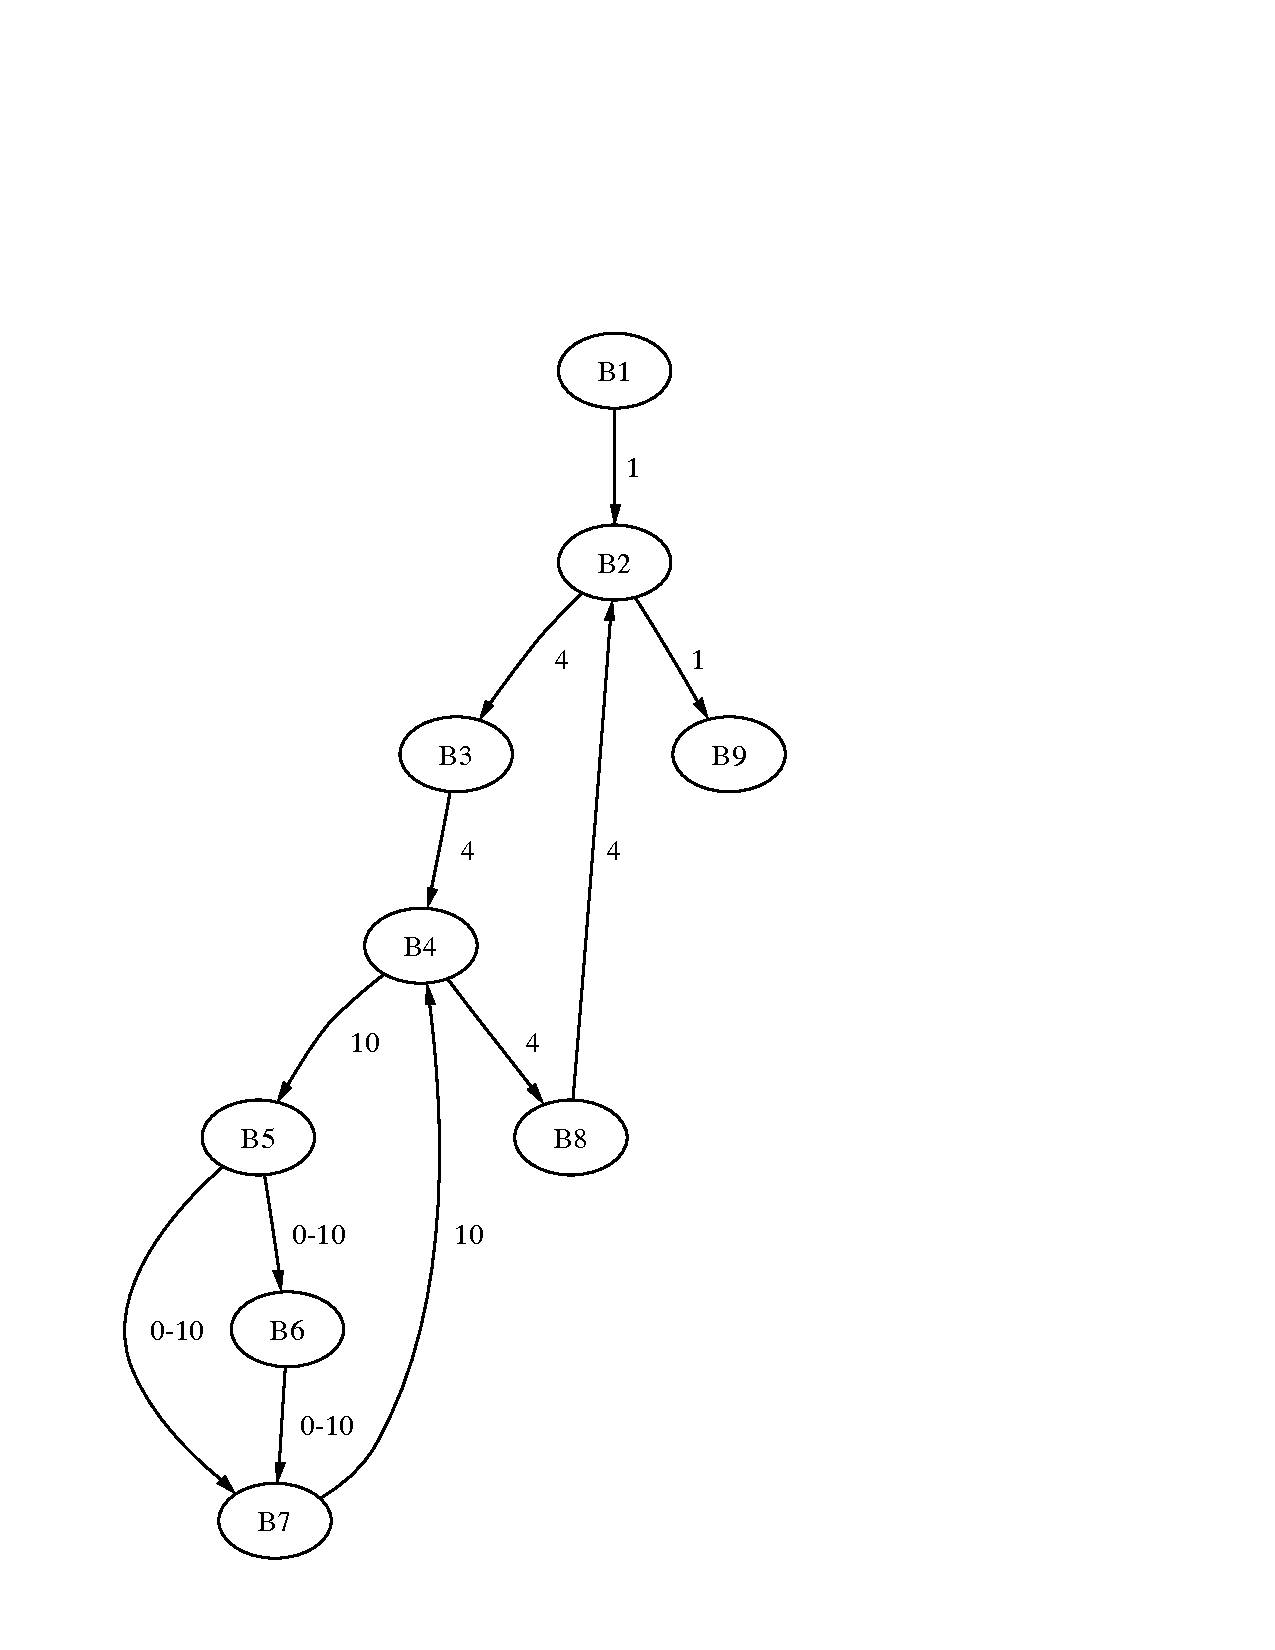
\includegraphics[height=\excelwidth]{results/results_wcet_cfg}
    \caption{The control flow graph of the Bubble Sort example}
    \label{fig:results:wcet:cfg}
\end{figure}

%The compiled version, i.e.\ the bytecodes of the test program, split
%into basic blocks, is given in
%\tablename~\ref{tab:results:bubble:wcet}. The fourth column contains
%the execution time of the bytecodes.


% the long table 'should' begin on a new page
%\pagebreak[4] %\pagebreak[3]
%{\footnotesize
%\begin{longtable}{lllr}
%    \toprule
%    Block & Addr. & Bytecode & Cycles \\
%    \midrule
%    \endhead
%    \caption{Bytecode listing of the Bubble Sort with basic blocks\label{tab:results:bubble:wcet}}
%    \endfoot
%    % table is two pages long, so don't use last caption in list
%    % of tables works
%    \caption[]{Bytecode listing of the Bubble Sort with basic blocks}
%    \endlastfoot
%    \input{bubble_instr}
%    \bottomrule
%\end{longtable}
%}


% this version fits in a two column A4 paper

%\begin{table}
%    \caption{Bytecode listing of the Bubble Sort with basic blocks}
%    \label{tab:results:bubble:wcet}
%\centering {\footnotesize
%\begin{tabular}{lllr}
%    \toprule
%    Block & Addr. & Bytecode & Cycles \\
%    \midrule
%    \input{bubble_instr}
%    \bottomrule
%\end{tabular}
%}
%\end{table}
%
\begin{table}
\centering
\begin{tabular*}{\columnwidth}{@{\extracolsep{\fill}}crrrrrr}
    \toprule
    & & &\multicolumn{2}{c}{WCET} & \multicolumn{2}{c}{BCET} \\
    Block & Addr. & Cycles & Count & Total & Count & Total \\
    \midrule
B1 & 0: &  2 &  1 &   2 &  1 &   2 \\
B2 & 2: &  5 &  5 &  25 &  5 &  25 \\
B3 & 6: &  2 &  4 &   8 &  4 &   8 \\
B4 & 8: &  6 & 14 &  84 & 14 &  84 \\
B5 &13: & 74 & 10 & 740 & 10 & 740 \\
B6 &30: & 73 & 10 & 730 &  0 &   0 \\
B7 &41: & 15 & 10 & 150 & 10 & 150 \\
B8 &47: & 15 &  4 &  60 &  4 &  60 \\
B9 &53: &    &  1 &     &  1 &     \\
\midrule
\multicolumn{4}{l}{Execution time calculated} & 1799  &    & 1069 \\
\multicolumn{4}{l}{Execution time measured}   & 1799  &    & 1069 \\
\bottomrule

\end{tabular*}
    \caption{WCET and BCET in clock cycles of the basic blocks}
    \label{tab:results:bubble:blocks}
\end{table}




In \tablename~\ref{tab:results:bubble:blocks} the basic blocks with
the start address (Addr.) and their execution time (Cycles) in clock
cycles and the worst and best case execution frequency (Count) is
given. The values in the forth and sixth columns (Count) of
\tablename~\ref{tab:results:bubble:blocks} are derived from the CFG
and show how often the basic blocks are executed in the worst and
best cases. The WCET and BCET value for each block is calculated by
multiplying the clock cycles by the execution frequency. The overall
WCET and BCET values are calculated by summing the values of the
individual blocks B1 to B8. The last block (B9) is omitted, as the
measurement does not contain the return statement.


The execution time of the program is measured using the cycle
counter in JOP. The current time is taken at both the entry of the
method and at the end, resulting in a measurement spanning from
block B1 to the beginning of block B9. The last statement, the
\code{return}, is not part of the measurement. The difference
between these two values (less the additional 8 cycles introduced by
the measurement itself) is given as the execution time in clock
cycles (the last row in \tablename~\ref{tab:results:bubble:blocks}).
The measured WCET and BCET values are exactly the same as the
calculated values.


In Figure~\ref{fig:results:wcet:sort}, the measured execution times
for all 120 permutations of the input data are shown. The vertical
axis shows the execution time in clock cycles and the horizontal
axis the number of the test run. The first input sample is an
already sorted array and results in the lowest execution time. The
last sample is the worst-case value resulting from the reversely
ordered input data. We can also see the 11 different execution times
that result from executing basic block B6 (which performs the
element exchange and takes 73 clock cycles) between 0 and 10 times.

\begin{figure}
    \centering
    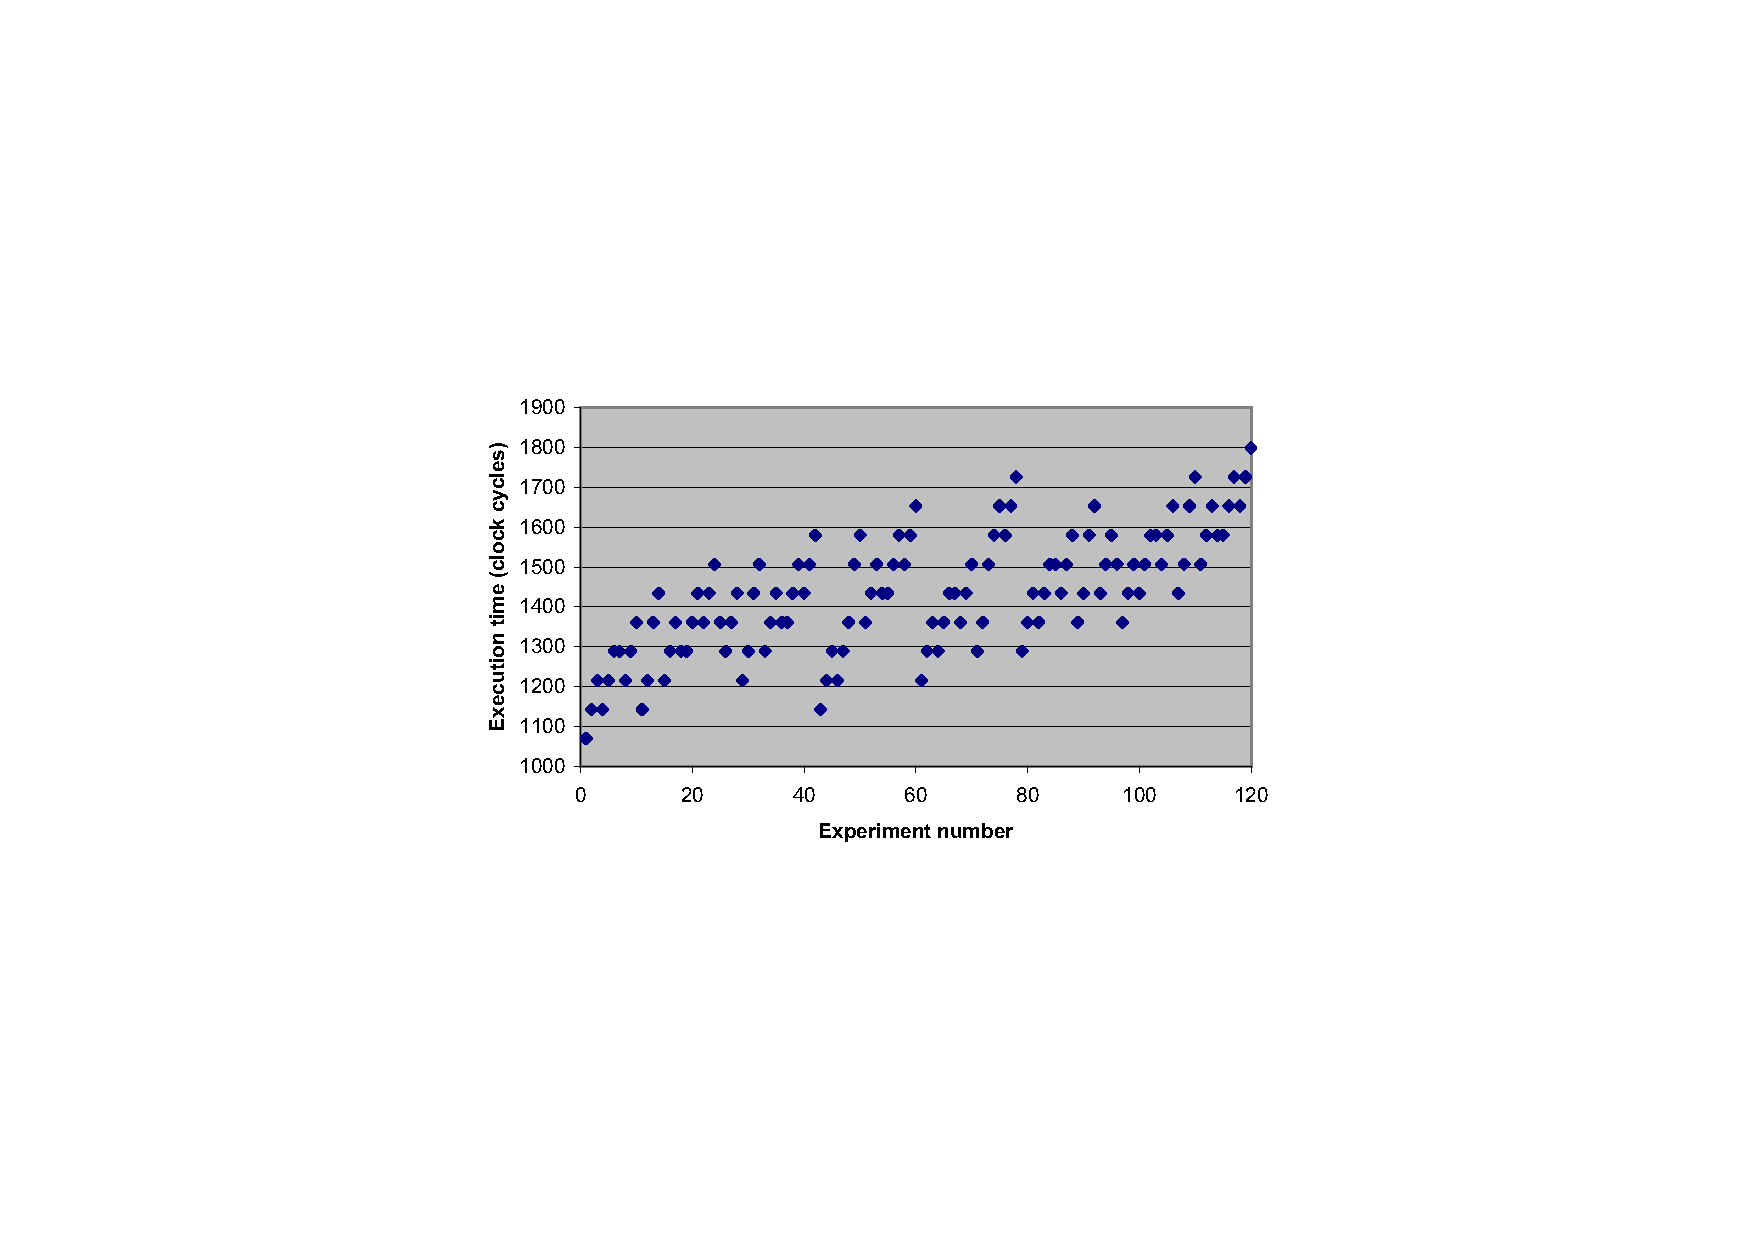
\includegraphics[width=\excelwidth]{results/results_wcet_sort}
    \caption{Execution time in clock cycles of the Bubble Sort program
    for all 120 permutations of the input data}
    \label{fig:results:wcet:sort}
\end{figure}




\subsection{WCET Analyzer} \label{sec:wcet:java}

In \cite{jop:wcet:jtres06} we have presented a static WCET analysis
tool for Java. During the high-level analysis the relevant
information is extracted from the class files. The control flow graph
(CFG) of the basic blocks\footnote{A basic block is a sequence of
instructions without any jumps or jump targets within this sequence.}
is extracted from the bytecodes. Annotations for the loop counts are
extracted from comments in the source. Furthermore, the class
hierarchy is examined to find all possible targets for a method
invoke.

The tool performs the low-level analysis at the bytecode level. The
behavior of the method cache is integrated for a simpler form (a two
block cache). The well known execution times of the different
bytecodes (see Section~\ref{sec:wcet:bc}) simplify this part of the
WCET analysis, which is usually the most complex one, to a great
extent. As there are no pipeline dependencies, the calculation of the
execution time for a basic block is merely just adding the individual
cycles for each instruction.

The actual calculation of the WCET is transformed to an integer
linear programming problem, a well known technique for WCET analysis
\cite{Puschner:JRTS1997,216666}. We performed the WCET analysis on
several benchmarks (see Table~\ref{tab:examples}). We also
\emph{measured} the WCET values for the benchmarks. It has to be
noted that we actually cannot measure the real WCET. If we could
measure it, we would not need to perform the WCET analysis at all.
The measurement gives us an idea of the pessimism of the analyzed
WCET.
%
\begin{table}
\centering {
\begin{tabular*}{\columnwidth}{@{\extracolsep{\fill}}llr}
    \toprule
    Program & Description & LOC \\
    \midrule
    \code{crc} & CRC calculation for short messages & 8 \\
    \code{robot} & A simple line follower robot & 111 \\
    \code{Lift} & A lift controler & 635 \\
    \code{Kfl} & \emph{Kippfahrleitung} application & 1366 \\
    \code{UdpIp} & UDP/IP benchmark & 1297 \\
    \bottomrule
\end{tabular*}
}
    \caption{WCET benchmark examples}
    \label{tab:examples}
\end{table}
%
The benchmarks \code{Lift} and \code{Kfl} are real-world examples
that are in industrial use. \code{Kfl} and \code{UdpIp} are also part
of an embedded Java benchmark suite that is used in
Section~\ref{sec:performance}.

Table~\ref{tab:wcet:compared} shows the measured execution time and
the analyzed WCET. The last column gives an idea of the pessimism of
the WCET analysis. For very simple programs, such as \code{crc} and
\code{robot}, the pessimism is quite low. For the \code{Lift}
example it is in an acceptable range.
%
\begin{table}
\centering {
\begin{tabular*}{\columnwidth}{@{\extracolsep{\fill}}lrrr}
    \toprule
%    & \multicolumn{2}{c}{WCET} & \\
            & Measured & Estimated & Pessimism\\
    Program & (cycle) & (cycle) & (ratio)\\
    \midrule
    \code{crc} & 1552 & 1620 & 1.04 \\
    \code{robot} & 736 & 775 & 1.05 \\
    \code{Lift} & 7214 & 11249 & 1.56 \\
    \code{Kfl} & 13334 & 28763 & 2.16 \\
    \code{UdpIp} & 11823 & 219569 & 18.57 \\
    \bottomrule
\end{tabular*}
}
    \caption{Measured and estimated WCETs with results in clock cycles}
    \label{tab:wcet:compared}
\end{table}
%
The difference between the measurement and the analysis in the
\code{Kfl} example results from the fact that our measurement does
not cover the WCET path. The large conservatism in \code{UdpIp}
results from the loop bound in the IP and UDP checksum calculation.
It is set for a 1500 byte packet buffer, but the payload in the
benchmark is only 8 bytes. The last two examples also show the issue
when a real-time application is developed without a WCET analysis
tool available.

The WCET analysis tool, with the help of loop annotations, provides
WCET values for the schedulability analysis. Besides the calculation
of the WCET, the tool provides user feedback by generating bytecode
listings with timing information and a graphical representation of
the CFG with timing and frequency information. This representation of
the WCET path through the code can guide the developer to write WCET
aware real-time code.

\section{Discussion}

The Bubble Sort example and experiments with the WCET analyzer tool
have demonstrated that we have achieved our goal: JOP is a simple
target for the WCET analysis. Most bytecodes have a single execution
time (WCET = BCET), and the WCET of a task (the analysis at the
bytecode level) depends only on the control flow. No pipeline or
data dependencies complicate the low-level part of the WCET
analysis.


The same analysis is not possible for other Java processors. Either
the information on the bytecode execution time is missing\footnote{We
tried hard to get this information for the aJile processor.} or some
processor features (e.g., the high variability of the latency for a
trap in picoJava) would result in very conservative WCET estimates.
Another example that prohibits exact analysis is the mechanism to
automatically fill and spill the stack cache in picoJava. The time
when the memory (cache) is occupied by this spill/fill action depends
on a long instruction history. Also the fill level of the
16-byte-deep prefetch buffer, which is needed for instruction
folding, depends on the execution history. All these automatic
buffering features have to be modeled quite conservatively. A
pragmatic solution is to assume empty buffers at the start of a basic
block. As basic blocks are quite short, most of the
buffering/prefetching does not help to lower the WCET.

Only for the Cjip processor is the execution time well documented
\cite{CjipRef}. However, as seen in Section~\ref{sec:perf:disc}, the
\emph{measured} execution time of some bytecodes is \emph{higher}
than the documented values. Therefore the documentation is not
complete to provide a safe processor model of the Cjip for the WCET
analysis.


\chapter{Low-level I/O}
\label{chap:io}
    \index{I/O access}

The following section describes the low-level mechanism for I/O
access and interrupts on JOP. As JOP is a Java processor no native
functions (usually written in C) are available to access I/O directly
or use C written interrupt handler. We need access to those low-level
functionality from Java for an embedded system. In the following a
hardware abstraction layer (HAL) in Java is proposed, where I/O
devices are mapped to Java objects and interrupt handlers can be
implemented in Java as \code{Runnable}. This section is based on
\cite{jop:hwobj} and \cite{jop:interrupt:handler}.


\section{Hardware Objects}
\label{sec:hwo} \index{hardware object}

Hardware objects map object fields to device registers. Therefore,
field access with bytecodes \code{putfield} and \code{getfield}
accesses device registers. With a correct class that represents a
device, access to it is safe -- it is not possible to read or write
to an arbitrary memory address. A memory area (e.g., a video frame
buffer) represented by an array is protected by Java's array bounds
check. Representing I/O devices as first class objects has following
benefits:

\begin{description}
    \item[Object-oriented:] An object representing a hardware
        device is the most natural integration into an OO
        language
    \item[Safe:] The safety of Java is not compromised. We can
        access only those device registers that are represented
        by the class definition
    \item[Efficient] Device register access is performed by
        single bytecodes \code{getfield} and \code{putfield}. We
        avoid expensive native calls.
\end{description}


\subsection{An Example}
\index{hardware object!example}

Let us consider a simple I/O device, e.g.\ a parallel input/output
(PIO) device -- a common device in embedded systems for control
applications. The PIO provides an interface between I/O registers and
I/O pins. The host captures data on the input pins with a register
read and drives data to the output pins with a register write. The
example PIO contains two registers: the \emph{data register} and the
\emph{control register}. Writing to the data register stores the
value into a register that drives the output pins. Reading from the
data register returns the value that is present at the input pins.

The control register configures the direction for each PIO pin. When
bit $n$ in the control register is set to 1, pin $n$ drives out the
value of bit $n$ of the data register. A 0 at bit $n$ in the control
register configures pin $n$ as input pin. At reset the port is
usually configured as input port -- a safe default
configuration.\footnote{Direction output can result in a short
circuit between the I/O pin and the external device when the logic
levels are different.}

\begin{lstlisting}[float=t,caption={Definition and usage of a parallel port in C},
label=lst:io:c:example]
    typedef struct {
        int data;
        int control;
    } parallel_port;

    #define PORT_ADDRESS 0x10000;

    int inval, outval;
    parallel_port *mypp;
    mypp = (parallel_port *) PORT_ADDRESS;
    ...
    inval = mypp->data;
    mypp->data = outval;
\end{lstlisting}

When the IO address space is memory mapped, such a parallel port is
represented in C as a structure and a constant for the address. This
definition is part of the board level configuration.
%It is provided by the board manufacturer or for configurable devices,
%such as FPGAs, generated by a system builder (e.g., Altera's
%\emph{SOPC Builder} \cite{quartus} for a NIOS system \cite{NIOS}).
Listing~\ref{lst:io:c:example} shows the parallel port example. The
parallel port is directly accessed via a pointer in C. For a system
with a distinct I/O address space (e.g.\ x86) access to the device
registers is performed via distinct machine instructions. Those
instructions are represented by C functions that take the address as
argument which is not type-safe.

This simple representation of memory mapped I/O devices in C is both
efficient and dangerous. It is efficient as the access via pointers
compiles to simple load and store instructions. It is dangerous as
wrong pointer manipulation can result in erroneous I/O or memory
access. This issue is inherent to C and C programmers are (hopefully)
aware of it. A major aspect that makes Java a safer\footnote{In this
context we consider the safety aspect as safe from programming
errors.} language than C is the avoidance of pointers. A pointer is
in effect an address to data manipulated as data -- an abstraction
that resembles more assembler programming than programming in a
high-level language.

On a standard JVM, native functions, written in C or C++, allow the
low-level access to devices from Java. This approach is not
object-oriented (OO) and incurs a lot of overheads; parameters and
return values have to be converted between Java and C. In an OO
language the most natural way to represent an I/O device is as an
object. Listing~\ref{lst:io:java:example} shows a class definition
for our simple parallel port.

\begin{lstlisting}[float=t,caption={The parallel port device as a simple Java class},
label=lst:io:java:example]
    public final class ParallelPort {
        public volatile int data;
        public volatile int control;
    }

    int inval, outval;
    myport = JVMMagic.getParallelPort();
    ...
    inval = myport.data;
    myport.data = outval;
\end{lstlisting}

The class \code{ParallelPort} is equivalent to the structure
definition for C in Listing~\ref{lst:io:c:example}. Reference
\code{myport} points to the hardware object. The device register
access is similar to the C version. The main difference to the C
structure is that the access requires no pointers. To provide this
convenient representation of I/O devices as objects we just need some
\emph{magic} in the JVM and a mechanism to \emph{create} the device
object and receive a reference to it.


\subsection{Definition}
\index{hardware object!definition}

All hardware classes have to extend the abstract class
\code{HardwareObject} (see Lising~\ref{lst:hwo:marker}). This empty
class serves as type marker. Some implementations use it to
distinguish between plain objects and hardware objects for the field
access. The package visible only constructor disallows creation of
hardware objects by the application code that resides in a different
package.

\begin{lstlisting}[float,caption={The marker class for hardware objects},
label=lst:hwo:marker]

public abstract class HardwareObject {
    HardwareObject() {};
}
\end{lstlisting}


Listing~\ref{lst:hwo:serial} shows a class representing a serial port
with a \code{status} register and a \code{data} register. The status
register contains flags for receive register full and transmit
register empty; the data register is the receive and transmit buffer.
Additionally, we define device specific constants (bit masks for the
\code{status} register) in the class for the serial port. All fields
represent device registers that can change due to activity of the
hardware device. Therefore, they must be declared \code{volatile}.

\begin{lstlisting}[float,caption={A serial port class with device methods},
label=lst:hwo:serial]

public final class SerialPort extends HardwareObject {

    public static final int MASK_TDRE = 1;
    public static final int MASK_RDRF = 2;

    public volatile int status;
    public volatile int data;

    public void init(int baudRate) {...}
    public boolean rxFull() {...}
    public boolean txEmpty() {...}
}
\end{lstlisting}

In this example we have included some convenience methods to access
the hardware object. However, for a clear separation of concerns, the
hardware object represents only the device state (the registers). We
do not add instance fields to represent additional state, i.e.,
mixing device registers with heap elements. We cannot implement a
complete device driver within a hardware object; instead a complete
device driver owns a number of private hardware objects along with
data structures for buffering, and it defines interrupt handlers and
methods for accessing its state from application processes. For
device specific operations, such as initialization of the device,
methods in hardware objects are useful.

\subsection{Access Control}

Usually each device is represented by exactly one hardware object
(see Section~\ref{sec:factory}). However, there might be use cases
where this restriction should be relaxed. Consider a device where
some registers should be accessed by system code only and some other
by application code. In JOP there is such a device: a system device
that contains a 1~MHz counter, a corresponding timer interrupt, and a
watchdog port. The timer interrupt is programmed relative to the
counter and used by the real-time scheduler -- a JVM internal
service. However, access to the counter can be useful for the
application code. Access to the watchdog register is required from
the application level. The watchdog is used for a sign-of-life from
the application. If not triggered every second the complete system is
restarted. For this example it is useful to represent one hardware
device by two \emph{different} classes -- one for system code and one
for application code. We can protect system registers by private
fields in the hardware object for the application.
Listing~\ref{lst:hwo:sys:classes} shows the two class definitions
that represent the same hardware device for system and application
code respectively. Note how we changed the access to the timer
interrupt register to \code{private} for the application hardware
object.

\begin{lstlisting}[float,caption={System and application classes
with visibility protection for a single hardware device},
label=lst:hwo:sys:classes]

public final class SysCounter extends HardwareObject {

    public volatile int counter;
    public volatile int timer;
    public volatile int wd;
}

public final class AppCounter extends HardwareObject {

    public volatile int counter;
    private volatile int timer;
    public volatile int wd;
}
\end{lstlisting}

Another option, shown in Listing~\ref{lst:hwo:sys:setget}, is to
declare all fields private for the application object and use setter
and getter methods. They add an abstraction on top of hardware
objects and use the hardware object to implement their functionality.
Thus we still do not need to invoke native functions.

\begin{lstlisting}[float,caption={System and application classes with setter and getter
methods}, label=lst:hwo:sys:setget]

public final class AppGetterSetter extends HardwareObject {

    private volatile int counter;
    private volatile int timer;
    private volatile int wd;

    public int getCounter() {
        return counter;
    }

    public void setWd(boolean val) {
        wd = val ? 1 : 0;
    }
}
\end{lstlisting}


\subsection{Using Hardware Objects}
\index{hardware object!usage}

Use of hardware objects is straightforward. After obtaining a
reference to the object all that has to be done (or can be done) is
to read from and write to the object fields.
Listing~\ref{lst:hwo:hello:world} shows an example of client code.
The example is a \emph{Hello World} program using low-level access to
a serial port via a hardware object.

\begin{lstlisting}[float=t,caption={A `Hello World' example with low-level device
access via a hardware object},
label=lst:hwo:hello:world]

import com.jopdesign.io.*;

public class Example {

    public static void main(String[] args) {

        BaseBoard fact = BaseBoard.getBaseFactory();
        SerialPort sp = fact.getSerialPort();

        String hello = "Hello World!";

        for (int i=0; i<hello.length(); ++i) {
            // busy wait on transmit buffer empty
            while ((sp.status & SerialPort.MASK_TDRE) == 0)
                ;
            // write a character
            sp.data = hello.charAt(i);
        }
    }
}
\end{lstlisting}


\subsection{Hardware Arrays}
\index{hardware object!arrays}

For devices that use DMA (e.g., video frame buffer, disk, and network
I/O buffers) we map that memory area to Java arrays. Arrays in Java
provide access to raw memory in an elegant way: the access is simple
and safe due to the array bounds checking done by the JVM. Hardware
arrays can be \emph{used} by the JVM to \emph{implement} higher-level
abstractions from the RTSJ such as \code{RawMemory} or scoped memory
\cite{jop:scope:cache}.

\subsection{Garbage Collection}

Interaction between the garbage collector (GC) and hardware objects
needs to be crafted into the JVM. We do not want to \emph{collect}
hardware objects. The hardware object should not be scanned for
references.\footnote{If a hardware coprocessor, represented by a
hardware object, itself manipulates an object on the heap and holds
the only reference to that object it has to be scanned by the GC.}
This is permissible when only primitive types are used in the class
definition for hardware objects -- the GC scans only reference
fields. To avoid collecting hardware objects, we \emph{mark} the
object to be skipped by the GC. The type inheritance from
\code{HardwareObject} can be used as the marker.

For JOP we only define hardware objects with primitive data fields.
Therefore, the hardware objects can be ignored by the GC. The GC
scans only objects where the handles are in the handle area. When the
GC is about to mark and scan an object it first checks if the
reference points into the handle area. If not, the reference is
skipped by the GC. All handles that lie outside of this area are
ignored by the GC. The handles for the hardware objects are allocated
in a special memory area (see Section~\ref{sec:hwo:implementation})
that is ignored by the GC. The same mechanism is already used by the
JVM for some runtime data structures (notable string constants) that
reside in their own memory area.

Handles which are not touched by the GC do not need the additional GC
info fields. We need only two fields: (1) the indirection field and
(2) the class reference or array length field.

\subsection{Hardware Object Creation} \label{sec:factory} \index{hardware object!creation}

The idea to represent each device by a single object or array is
straightforward, the remaining question is: How are those objects
created? An object that represents a device is a typical Singleton
\cite{Go4}. Only a single object should map to one instance of a
device. Therefore, hardware objects cannot be instantiated by a
simple \code{new}: (1) they have to be mapped by some JVM mechanism
to the device registers and (2) each device instance is represented
by a single object.

Each device object is created by its own factory method. The
collection of these methods is the board configuration, which itself
is also a Singleton (the application runs on a single board). The
Singleton property of the configuration is enforced by a class that
contains only static methods. Listing~\ref{lst:hwo:static:fact} shows
an example for such a class. The class \code{IOSystem} represents a
system with three devices: a parallel port, as discussed before to
interact with the environment, and two serial ports: one for program
download and one which is an interface to a GPS receiver.

\begin{lstlisting}[float=t,caption={A factory with static methods for Singleton hardware objects},
label=lst:hwo:static:fact]

package com.board-vendor.io;

public class IOSystem {

    // some JVM mechanism to create the hardware objects
    private static ParallelPort pp = jvmPPCreate();
    private static SerialPort sp = jvmSPCreate(0);
    private static SerialPort gps = jvmSPCreate(1);

    public static ParallelPort getParallelPort() {
        return pp;
    }

    public static SerialPort getSerialPort() {..}
    public static SerialPort getGpsPort() {..}
}
\end{lstlisting}


This approach is simple, but not very flexible. Consider a vendor who
provides boards in slightly different configurations (e.g., with
different number of serial ports). With the above approach each board
requires a different (or additional) \code{IOSystem} class that lists
all devices. A more elegant solution is proposed in the next section.

\subsection{Board Configurations}
\index{hardware object!board configuration}

Replacing the static factory methods by instance methods avoids code
duplication; inheritance then gives configurations. With a factory
object we represent the common subset of I/O devices by a base class
and the variants as subclasses.

However, the factory object itself must still be a Singleton.
Therefore the board specific factory object is created at class
initialization and is retrieved by a static method.
Listing~\ref{lst:hwo:base:fact} shows an example of a base factory
and a derived factory. Note how \code{getBaseFactory()} is used to
get a single instance of the factory. We have applied the idea of a
factory two times: the first factory generates an object that
represents the board configuration. That object is itself a factory
that generates the objects that interface to the hardware device.

\begin{lstlisting}[float=t,caption={A base class of a hardware object
factory}, label=lst:hwo:base:fact]

public class BaseBoard {

    private final static int SERIAL_ADDRESS = ...;
    private SerialPort serial;
    BaseBoard() {
        serial = (SerialPort) jvmHWOCreate(SERIAL_ADDRESS);
    };
    static BaseBoard single = new BaseBoard();
    public static BaseBoard getBaseFactory() {
        return single;
    }
    public SerialPort getSerialPort() { return serial; }

    // here comes the JVM internal mechanism
    Object jvmHWOCreate(int address) {...}
}
\end{lstlisting}

The shown example base factory represents the minimum configuration
with a single serial port for communication (mapped to
\code{System.in} and \code{System.out}) represented by a
\code{SerialPort}. The derived configuration \code{ExtendedBoard}
(listing~\ref{lst:hwo:ext:fact}) contains an additional serial port
for a GPS receiver and a parallel port for external control.

\begin{lstlisting}[float=t,caption={An extended class of a hardware object
factory for a board variation}, label=lst:hwo:ext:fact]

public class ExtendedBoard extends BaseBoard {

    private final static int GPS_ADDRESS = ...;
    private final static int PARALLEL_ADDRESS = ...;
    private SerialPort gps;
    private ParallelPort parallel;
    ExtendedBoard() {
        gps = (SerialPort) jvmHWOCreate(GPS_ADDRESS);
        parallel = (ParallelPort) jvmHWOCreate(PARALLEL_ADDRESS);
    };
    static ExtendedBoard single = new ExtendedBoard();
    public static ExtendedBoard getExtendedFactory() {
        return single;
    }
    public SerialPort getGpsPort() { return gps; }
    public ParallelPort getParallelPort() { return parallel; }
}
\end{lstlisting}



%% MS: we have two different static methods getXXFactory() - could we use one name?
% is this kind of 'overloading' (more hiding) allowed in Java?
% APR its is OK if the signatures are different

Furthermore, we show in those examples a different way to incorporate
the JVM mechanism in the factory: we define well known constants (the
memory addresses of the devices) in the factory and let the native
function \code{jvmHWOCreate()} return the correct device type.

%Figure~\ref{fig:uml} gives a summary example of hardware object
%classes and the corresponding factory classes as a UML class diagram.
%The figure shows that all device classes subclass the abstract class
%\code{HardwareObject}.
%
%\begin{figure}
%    \centering
%    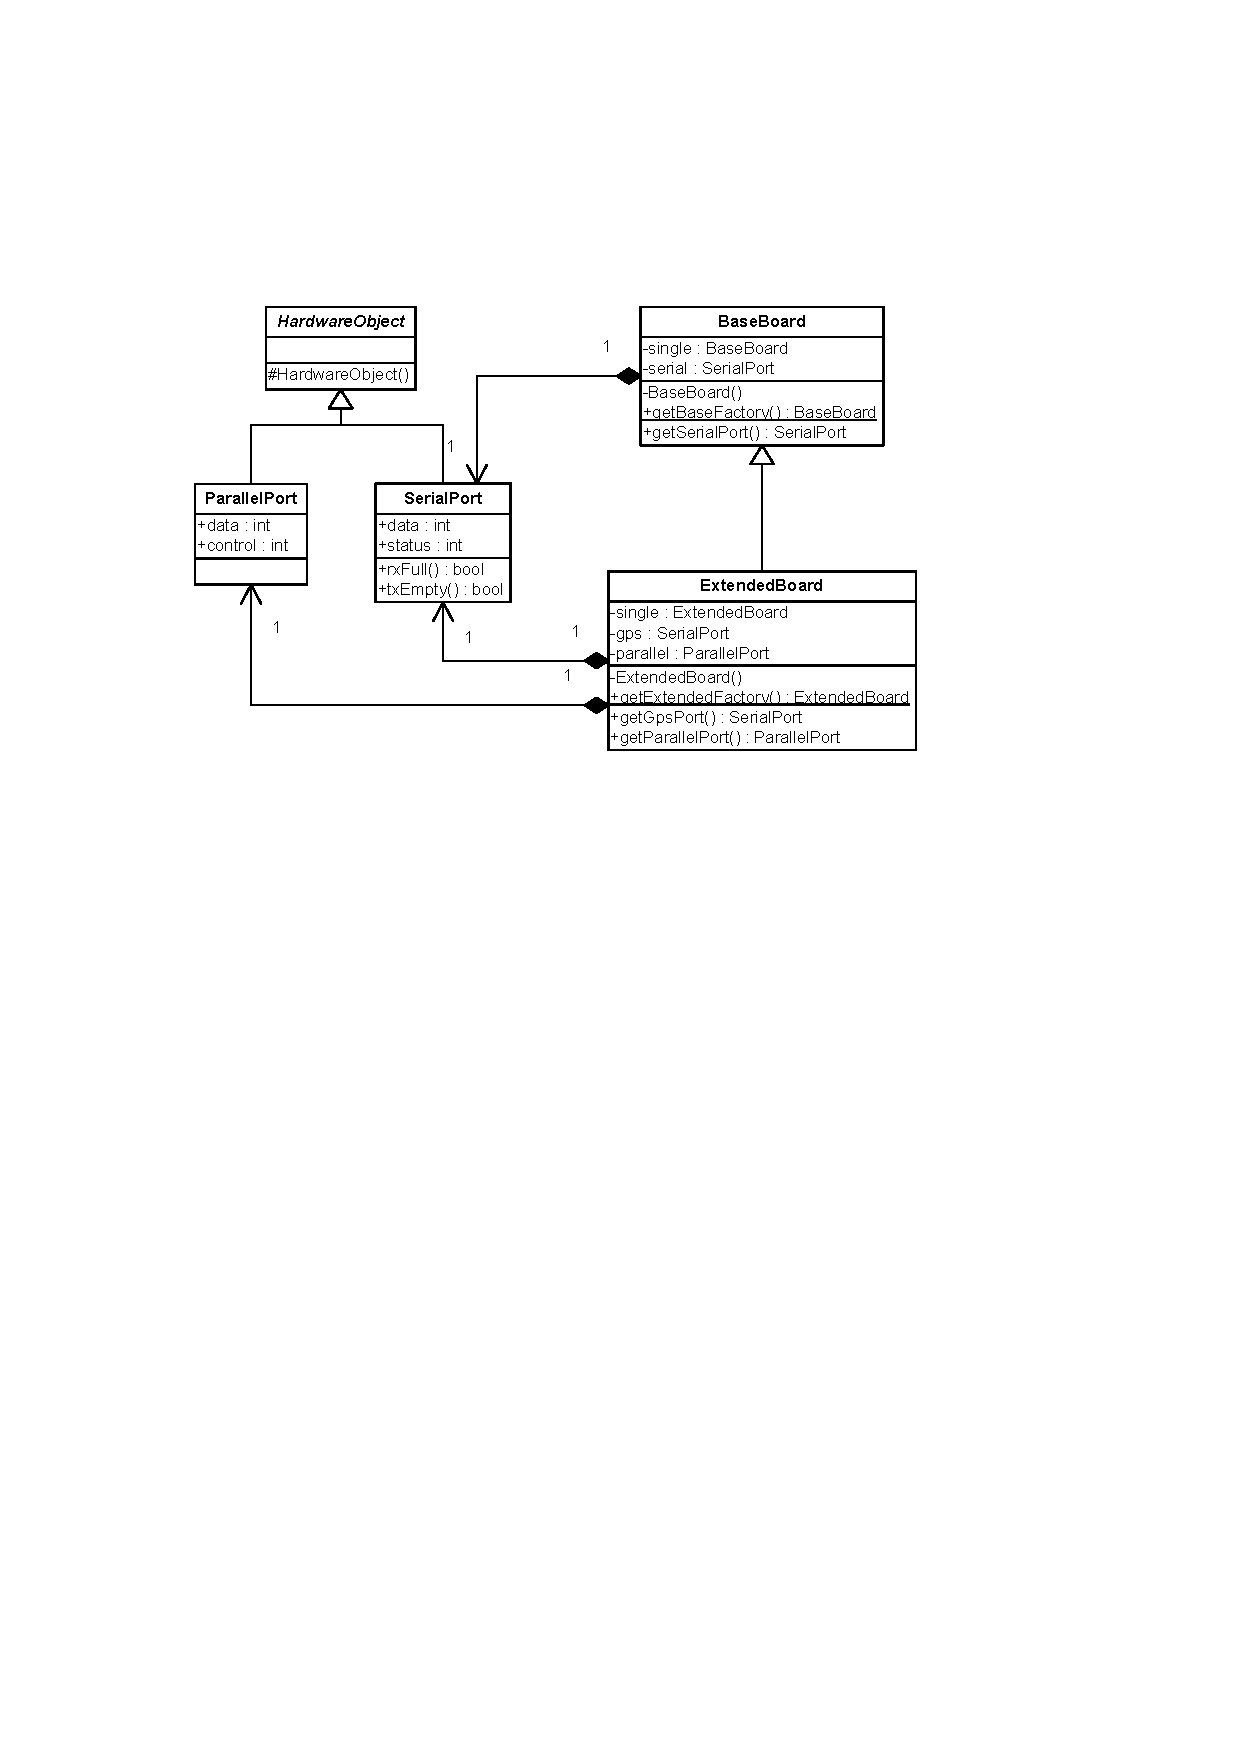
\includegraphics[scale=0.8]{io/uml}
%   \caption{Device object classes and board factory classes}\label{fig:uml}
%\end{figure}
%

\subsection{Implementation}
\label{sec:hwo:implementation} \index{hardware object!implementation}

In this subsection the internals of the hardware object creation are
described. Just to use hardware objects this section can be skipped.
To create new types of hardware objects and the companion factory
this section contains the needed details.

\begin{figure}[t]
    \centering
    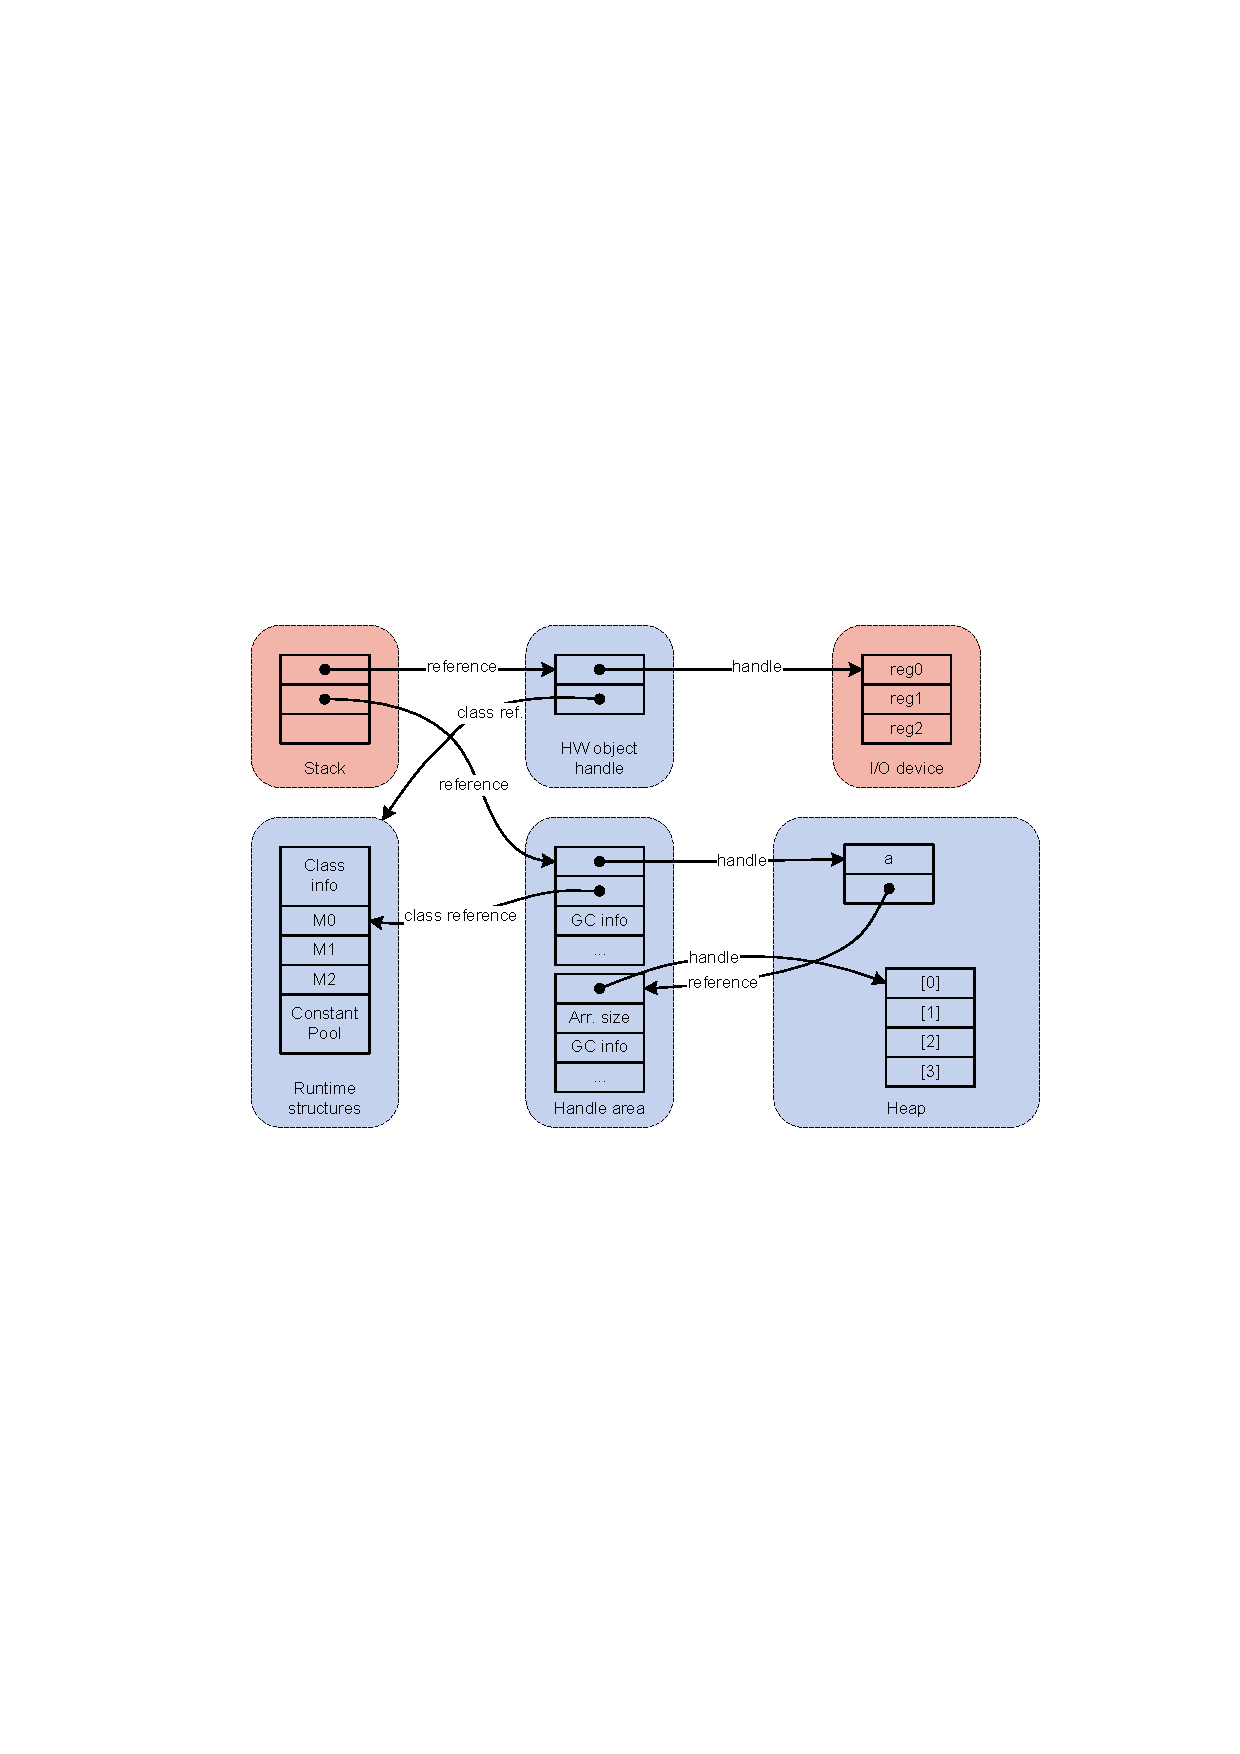
\includegraphics[scale=\picscale]{io/memory}
    \caption{Memory layout of the JOP JVM}\label{fig:hwo:mem}
\end{figure}

In JOP, objects and arrays are referenced through an indirection
called \emph{handle}. This indirection is a lightweight read barrier
for the compacting real-time GC (see Chapter~\ref{chap:rtgc}). All
handles for objects in the heap are located in a distinct memory
region, the handle area. Besides the indirection to the \emph{real}
object the handle contains auxiliary data, such as a reference to the
class information, the array length, and GC related data.
Figure~\ref{fig:hwo:mem} shows an example with a small object that
contains two fields and an integer array of length 4. The object and
the array on the heap just contain the data and no additional hidden
fields. This object layout greatly simplifies our object to device
mapping. We just need a handle where the indirection points to the
memory mapped device registers instead of into the heap. This
configuration is shown in the upper part of Figure~\ref{fig:hwo:mem}.
Note that we do not need the GC information for the hardware object
handles. The factory, which creates the hardware objects, implements
this indirection.

As described in Section~\ref{sec:factory} we do not allow
applications to create hardware objects; the constructor is private
(or package visible).\footnote{For creation of hardware objects with
\codefoot{new} we would need to change the implementation of bytecode
\codefoot{new} to distinguish between normal heap allocated objects
and hardware objects. In the implementation on JOP the hardware
object constructor is package visible to allow the factory to create
a plane object of that type.} Listing~\ref{lst:hwo:jop:base} shows
part of the base hardware object factory that creates the hardware
object \code{SerialPort} and \code{SysDevice}. Two static fields
(\code{SP\_PTR} and \code{SP\_MTAB}) are used to store the handle to
the serial port object. The first field is initialized with the base
address of the I/O device; the second field contains a pointer to the
class information.\footnote{In JOP's JVM the class reference is a
pointer to the method table to speed-up the invoke instruction.
Therefore, the name is \codefoot{XX\_MTAB}.} The address of the
static field \code{SP\_PTR} is returned as the reference to the
serial port object.

\begin{lstlisting}[caption={Simplified version of the JOP base factory},
label=lst:hwo:jop:base]

public class IOFactory {
    private SerialPort sp;
    private SysDevice sys;

    // Handles should be the first static fields!
    private static int SP_PTR;
    private static int SP_MTAB;
    private static int SYS_PTR;
    private static int SYS_MTAB;

    IOFactory() {
        sp = (SerialPort) makeHWObject(new SerialPort(), Const.IO_UART1_BASE, 0);
        sys = (SysDevice) makeHWObject(new SysDevice(), Const.IO_SYS_DEVICE, 1);
    };
    // that has to be overridden by each sub class to get the correct cp
    private static Object makeHWObject(Object o, int address, int idx) {
        int cp = Native.rdIntMem(Const.RAM_CP);
        return JVMHelp.makeHWObject(o, address, idx, cp);
    }
    private static IOFactory single = new IOFactory();
    public static IOFactory getFactory() {
        return single;
    }

    public SerialPort getSerialPort() { return sp; }
    public SysDevice getSysDevice() { return sys; }
}
\end{lstlisting}

The class reference for the hardware object is obtained by creating a
\emph{normal} instance of \code{SerialPort} with \code{new} on the
heap and copying the pointer to the class information. To avoid using
native methods in the factory class we delegate JVM internal work to
a helper class in the JVM system package as shown in
Listing~\ref{lst:hwo:helper}. That helper method returns the address
of the static field \code{SP\_PTR} as reference to the hardware
object. All methods in class \code{Native}, a JOP system class, are
\emph{native}\footnote{There are no \emph{real} native functions in
JOP -- bytecode is the native instruction set. The very few native
methods in class \codefoot{Native} are replaced by special, unused
bytecodes during class linking.} methods for low-level functions --
the code we want to avoid in application code. Method
\code{toInt(Object o)} defeats Java's type safety and returns a
reference as an \code{int}. Method \code{toObject(int addr)} is the
inverse function to map an address to a Java reference. Low-level
memory access methods are used to manipulate the JVM data structures.

\begin{lstlisting}[float,caption={The helper method in the system class \code{JVMHelp} for the hardware object
creation}, label=lst:hwo:helper]

public static Object makeHWObject(Object o, int address, int idx, int
cp) {
    int ref = Native.toInt(o);
    int pcl = Native.rdMem(ref+1);
    int p = Native.rdMem(cp-1);
    p = Native.rdMem(p+1);
    p += idx*2;
    Native.wrMem(address, p);
    Native.wrMem(pcl, p+1);
    return Native.toObject(p);
}
\end{lstlisting}

To disallow the creation with \code{new} in normal application code,
the visibility is set to package. The package visibility of the
hardware object constructor is a minor issue.
%
%% MS: not anymore - code is removed
%The work-around to retrieve the address of a static field from a
%class in Java code is also shown in Listing~\ref{fig:hwobj:helper}.
%%
%% MS: this section contains too much details on JOP.
%% Perhaps remove it.
%%
%
%We want to group all I/O device classes and the Factory classes,
%which describe different boards, in a single package, in our case in
%\code{com.jopdesign.io}. As we have seen in the former section we
%need some native functions in the factory methods. The native
%functions for JOP (class \code{Native}) are located in a system
%package (\code{com.jopdesign.sys}). This system package contains JVM
%internal classes for scheduling, garbage collection, and JVM helper
%methods. As Java does not contain the \emph{friend} construct from
%C++ we have to declare the native functions public -- something we
%wanted to avoid by our hardware objects.
%
%Moving the Factory classes to the system package is not an option:
%(1) we would need to set the visibility of the hardware object
%constructor to \code{public} and (2) splitting the I/O classes into
%two packages is not a good design decision. A solution -- or better
%work-around -- is delegating some Factory work to a helper method in
%the system package. Listing~\ref{lst:hwo:helper} shows the Factory
%constructor. Helper method \code{JVMHelp.makeHWObject()} contains the
%instructions to read the class information reference from an object.
%
To access private static fields of an arbitrary class from the system
class we had to change the runtime class information: we added a
pointer to the first static primitive field of that class. As
addresses of static fields get resolved at class linking, no such
reference was needed so far.

\subsection{Legacy Code}

Before the implementation of hardware objects, the access to I/O
devices was performed with memory read and write methods. Those
methods are \code{Native.rdMem()} and \code{Native.wrMem()}. Due to
historical reasons\footnote{In an older version of JOP I/O and memory
had different busses.} the same Methods also exist as
\code{Native.rd()} and \code{Native.wr()}.

Those native methods are mapped to a system bytecode and perform
direct memory access -- not a save abstraction at all. However, there
exists still some Java code that uses those public visible methods.
Those methods are depreciated and new device drivers shall use
hardware objects.

\section{Interrupt Handlers}

\index{interrupt!handler}

Interrupts are notifications from hardware components to the
processor. As a response to the interrupt signal some method needs to
be invoked and executed. To allow implementation of first-level
interrupt handler (IH) in Java we map interrupt requests to
invocations of the \code{run()} method of a \code{Runnable}.
Listing~\ref{lst:io:int:example} shows an example of such an
interrupt handler and how it is registered.

\begin{lstlisting}[caption={A simple first-level interrupt handler in Java},
label=lst:io:int:example]

public class InterruptHandler implements Runnable {

    public static void main(String[] args) {

        // get factory
    	InterruptHandler ih = new InterruptHandler();
    	fact.registerInterruptHandler(1, ih);
    	
    	// enable interrupt 1
    	fact.enableInterrupt(1);

        // start normal work
    }

    public void run() {
    	// do the first level interrupt handler work
    }

}
\end{lstlisting}

\subsection{Synchronization}

\index{interrupt!synchronization}

When an interrupt handler is invoked, it starts with global interrupt
disabled. The global interrupt mask is enabled again when the
interrupt handler returns. On the uniprocessor version of JOP the
monitor is also implemented by simply masking all interrupts.
Therefore, those critical sections cannot be interrupted and
synchronization between the interrupt handler and a normal thread is
fulfilled. For a CMP version of JOP synchronization is performed via
a global hardware lock. As the CMP system offers true concurrency,
the IH has to protect the access to shared data when the handler and
the thread are located on different cores.

A better approach for data sharing between a first-level IH and a
device driver task (or second-level IH) is the usage of non-blocking
queues.  Listing~\ref{lst:hwo:nonbl:buffer} shows an example of such
a bonded, non-blocking buffer for single reader and single writer
communication. The class \code{Buffer} is part of the package
\code{rtlib}.

\index{non-blocking queue} \index{interrupt!non-blocking queue}

\begin{lstlisting}[caption={A non-blocking integer buffer for a
single reader and a single writer. Classical usage is in an interrupt
handler.}, label=lst:hwo:nonbl:buffer]

public class Buffer {

    private volatile int[] data;
    private volatile int rdPtr;
    private volatile int wrPtr;

    public Buffer(int size) {
        data = new int[size+1];
        rdPtr = wrPtr = 0;
    }
    public boolean empty() {
        return rdPtr==wrPtr;
    }
    public boolean full() {
        int i = wrPtr+1;
        if (i>=data.length) i=0;
        return i==rdPtr;
    }
    public int read() {
        int i =rdPtr;
        int val = data[i++];
        if (i>=data.length) i=0;
        rdPtr = i;
        return val;
    }
    public void write(int val) {
        int i = wrPtr;
        data[i++] = val;
        if (i>=data.length) i=0;
        wrPtr = i;
    }
    public int cnt() {
        int i = wrPtr-rdPtr;
        if (i<0) i+=data.length;
        return i;
    }
    public int free() {
        return data.length-1-cnt();
    }
    public int checkedRead() {
        if (empty()) return -1;
        return read();
    }
    public boolean checkedWrite(int val) {
        if (full()) return false;
        write(val);
        return true;
    }
}
\end{lstlisting}


The buffer \code{data} is manipulated by the reader and writer. The
size of the buffer is determined by the constructor. The read pointer
\code{rdPtr} is only manipulated by the reader, the write pointer
\code{wrPtr} only by the writer. The buffer is empty when
\code{rdPtr} equals \code{wrPtr} and full when \code{wrPtr}+1 equals
the \code{rdPtr}. In method \code{full()} two points are notable: (1)
the usage of the local variable to get an atomic snapshot of the
\code{wrPtr}; and (2) the usage of $>=$ instead of $=$ for easier
data-flow analysis \cite{dfa:puffitsch:2009}.

The methods \code{read()} and \code{write()} perform an unchecked
read and write from the buffer -- the unchecked version is for
performance reason. Therefore, before invoking those methods the
buffer fill state has to be checked with \code{emtpy()} and
\code{full()}. If read is performed on an empty buffer, the buffer is
corrupted -- old, alread read data appears as new data. Write to a
full buffer drops all former data. The fill stat of the buffer can be
queried with \code{cnt()} and \code{free()}. Method
\code{checkedRead()} reads one entry from the buffer or returns -1 if
the buffer is empty. Method \code{checkedWrite()} write one entry
into the buffer when not full and returns \code{true} if the write
operation was successfully.

An object oriented version of this single reader/writer queue is
available in class \code{SRSWQueue}.  Those queues are also handy for
communication between threads as blocking can be avoided. The
redesigned TCP/IP stack \code{ejip} uses those non-blocking queues
for communication of network packets between different protocol
layers.

\subsection{Interrupt Handler Registration}

Interrupt handlers can be registered for a interrupt number $n$. On
the CMP system the interrupt is registered on the core where the
method is invoked. Following methods are available in the factory
class for interrupt handler registration/deregistration and
enable/disable of a specific interrupt.

\begin{samepage}
\begin{lstlisting}
    public void registerInterruptHandler(int nr, Runnable logic) { }
    public void deregisterInterruptHandler(int nr) { }
    public void enableInterrupt(int nr) { }
    public void disableInterrupt(int nr) { }
\end{lstlisting}
\end{samepage}

Interrupt 0 has a special meaning as it is the reprogrammable timer
interrupt for the scheduler. On the transition to the mission phase
(\code{startMission()}) a scheduler, which is a simple
\code{Runable}, is registered for each core for the timer interrupt.

\subsection{Implementation}

\index{interrupt!implementation}

The original JOP \cite{jop:thesis,jop:jnl:jsa2007} was a very
puristic hard real-time processor. There existed only one interrupt
-- the programmable timer interrupt as time is the primary source for
hard real-time events. All I/O requests were handled by periodic
threads that poll for pending input data or free output buffers.
However, to allow a more flexible programming model additional
hardware interrupts are now available.

On a pending interrupt (or exception generated by the hardware) a
special bytecode is inserted into the instruction stream (see
Section~\ref{sec:interrupt}. This approach keeps the interrupt
completely transparent to the core pipeline. The special bytecode
that is unused by the JVM specification \cite{jvm} is used to invoke
the special method \code{interrupt()} from the JVM helper class
\code{JVMHelp}.

The implemented interrupt controller (IC) is priority based. The
number of interrupt sources can be configured. Each interrupt can be
triggered in software by a IC register write as well. There is one
global interrupt enable and each interrupt line can be enabled or
disabled locally. The interrupt is forwarded to the
bytecode/microcode translation stage with the interrupt number. When
accepted by this stage, the interrupt is acknowledged and the global
enable flag cleared. This feature avoids immediate handling of an
arriving higher priority interrupt during the first part of the
handler. The interrupts have to be enabled again by the handler at a
\emph{convenient} time. All interrupts are mapped to the same special
bytecode. Therefore, we perform the dispatch of the correct handler
in Java. On an interrupt the static method \code{interrupt()} from a
system internal class gets invoked. The method reads the interrupt
number and performs the dispatch to the registered \code{Runnable} as
illustrated below. Note, how a hardware object of type
\code{SysDevice} is used to read the interrupt number.

\index{interrupt!dispatch}

\begin{samepage}
\begin{lstlisting}
    static Runnable ih[] = new Runnable[Const.NUM_INTERRUPTS];
    static SysDevice sys = IOFactory.getFactory().getSysDevice();

    static void interrupt() {
        ih[sys.intNr].run();
    }
\end{lstlisting}
\end{samepage}

The timer interrupt, used for the real-time scheduler, is located at
index 0. The scheduler is just a plain interrupt handler that gets
registered at mission start at index 0. At system startup, the table
of Runnables is initialized with dummy handlers. The application code
provides the handler via a class that implements \code{Runnable} and
registers that class for an interrupt number.

For interrupts that should be handled by an event handler under the
control of the scheduler, the following steps need to be performed on
JOP:
\begin{enumerate}
  \item Create a \code{SwEvent} with the correct priority that
      performs the second level interrupt handler work
  \item Create a short first level interrupt handler as
      \code{Runnable} that invokes \code{fire()} of the
      corresponding software event handler
  \item Register the first level interrupt handler as shown in
      Figure~\ref{fig:ihjop} and start the real-time scheduler
\end{enumerate}


\subsection{An Example}

The system device (\code{sc\_sys.vhd}) contains input lines for
external interrupts (in port \code{io\_int}). The number of interrupt
lines is configurable with \code{num\_io\_int}. Each hardware
interrupt can also be triggered by a write into the system device.
Listing~\ref{lst:hwo:full:example} shows registering and using a
first level interrupt handler. The interrupt is triggered in software
by the main thread.

\begin{lstlisting}[caption={Interrupt register/deregister methods in the factory class},
label=lst:hwo:full:example]

public class InterruptHandler implements Runnable {

    public static void main(String[] args) {

        IOFactory fact = IOFactory.getFactory();
        SysDevice sys = fact.getSysDevice();

        InterruptHandler ih = new InterruptHandler();
        fact.registerInterruptHandler(1, ih);

        // enable software interrupt 1
        fact.enableInterrupt(1);

        for (int i=0; i<20; ++i) {
            Timer.wd();
            int t = Timer.getTimeoutMs(200);
            while (!Timer.timeout(t)) ;
            // trigger a SW interrupt via the system HW object
            System.out.println("Trigger");
            sys.intNr = 1;
            if (i==10) {
                fact.disableInterrupt(1);
            }
        }
    }

    public void run() {
        System.out.println("Interrupt fired!");
    }
}
\end{lstlisting}


\section{Standard Devices}

A minimum version of JOP consists of two standard devices: the system
device and a UART device for program download and as a representation
of \code{System.ou}.

\subsection{The System Device}

\index{system device}

The system device contains all the logic for interrupts, CMP
interaction, timers, and the watchdog control. The registers
definition is shown in Table~\ref{tab:io:sysdev}.

\begin{table}[t]
    \centering
    \begin{tabular}{cll}
        \toprule
        Address  & Read & Write \\
        \midrule
        0 & Clock counter & Interrupt enable \\
        1 & Counter in $\mu$s & Timer interrupt in $\mu$s \\
        2 & Interrupt number & SW interrupt \\
        3 & --- & Watchdog \\
        4 & Exception reason & Generate exception \\
        5 & Lock request status & Lock request \\
        6 & CPU ID & --- \\
        7 & Polled in JVM startup & Start CMP \\
        8 & --- & Interrupt mask \\
        9 & --- & Clear pending interrupts \\
        11 & Nr. CPUs & --- \\
        \bottomrule
    \end{tabular}
    \caption{Registers in the system device.}
    \label{tab:io:sysdev}
\end{table}

\subsection{The UART}

The UART contains a contral/status register and a data read/write
register is shown in Table~\ref{tab:io:uart}.

\begin{table}[t]
    \centering
    \begin{tabular}{cll}
        \toprule
        Address  & Read & Write \\
        \midrule
        0 & status & control \\
        1 & receive data & transmit buffer \\
        \bottomrule
    \end{tabular}
    \caption{Registers in the UART device.}
    \label{tab:io:uart}
\end{table}


\chapter{The SimpCon Interconnect}
\label{chap:simpcon}
\newcommand{\scgrsc}{.65}
\newcommand{\scgrp}{simpcon}
\hyphenation{SimpCon}
SimpCon \cite{simpcon} is the main interconnection interface used
for JOP. The IO modules and the main memory are connected via this
standard. In the following chapter an introduction to SimpCon is
presented.

The VHDL files in \dirent{vhdl/scio} are SimpCon IO components
(e.g.\ \code{sc\_uart.vhd} is a simple UART) and SimpCon IO
configurations. The IO configurations define the IO devices and the
address mapping for a JOP system. All those configurations start
with \code{scio\_}. The IO components start with \code{sc\_}.
Configuration \code{scio\_min} contains the minimal IO components
for a JOP system: the system module \code{sc\_sys.vhd} and a UART
\code{sc\_uart.vhd} for program download and basic communication
(\code{System.in} and \code{System.out}).

The system module \code{sc\_sys.vhd} contains the clock counter, the
$\mu$s counter, timer interrupt, the SW interrupt, exception
interrupts, the watchdog port, and the connection to the
multiprocessor synchronization unit (\code{cmpsync.vhd}).

In directory \dirent{vhdl/memory} the memory controller
\code{mem\_sc.vhd} is a SimpCon master that can be connected to
various SRAM memory controllers \code{sc\_sram*.vhd}. Other memory
controller (e.g.\ the free Altera SDRAM interface) can be connected
via SimpCon bridges to Avalon, Wishbone, and AHB slave (available in
\dirent{vhdl/simpcon}).


\section{Introduction}

The intention of the following SoC interconnect standard is to be
simple and efficient with respect to implementation resources and
transaction latency.

SimpCon is a fully synchronous standard for on-chip
interconnections. It is a point-to-point connection between a master
and a slave. The master starts either a read or write transaction.
Master commands are single cycle to free the master to continue on
internal operations during an outstanding transaction. The slave has
to register the address when needed for more than one cycle. The
slave also registers the data on a read and provides it to the
master for more than a single cycle. This property allows the master
to delay the actual read if it is busy with internal operations.

The slave signals the end of the transaction through a novel
\emph{ready counter} to provide an early notification. This early
notification simplifies the integration of peripherals into
pipelined masters.

Slaves can also provide several levels of pipelining. This feature
is announced by two static output ports (one for read and one write
pipeline levels).

Off-chip connections (e.g.\ main memory) are device specific and
need a slave to perform the translation. Peripheral interrupts are
not covered by this specification.

\subsection{Features}

\begin{itemize}
    \item Master/slave point-to-point connection
    \item Synchronous operation
    \item Read and write transactions
    \item Early pipeline release for the master
    \item Pipelined transactions
    \item Open-source specification
    \item Low implementation overheads
\end{itemize}

\subsection{Basic Read Transaction}

Figure~\ref{fig:sc:basic:rd} shows a basic read transaction for
a slave with one cycle latency. The acknowledge signals are
omitted from the figure. In the first cycle, the address phase,
the \sign{rd} signals the slave to start the read transaction.
The address is registered by the slave. During the following
cycle, the read phase\footnote{It has to be noted that the read
phase can be longer for devices with a high latency. For simple
on-chip IO devices the read phase can be omitted completely (0
cycles). In that case \sign{rdy\_cnt} will be zero in the cycle
following the address phase.}, the slave performs the read and
registers the data. Due to the register in the slave the data
is available in the third cycle, the result phase. To simplify
the master, \sign{rd\_data} stays valid till the next read
request response. It is therefore possible for a master to
issue a pre-fetch command early. When the pre-fetched data
arrives to early it is still valid when the master actually
wants to read it.

\begin{figure}
    \centering
    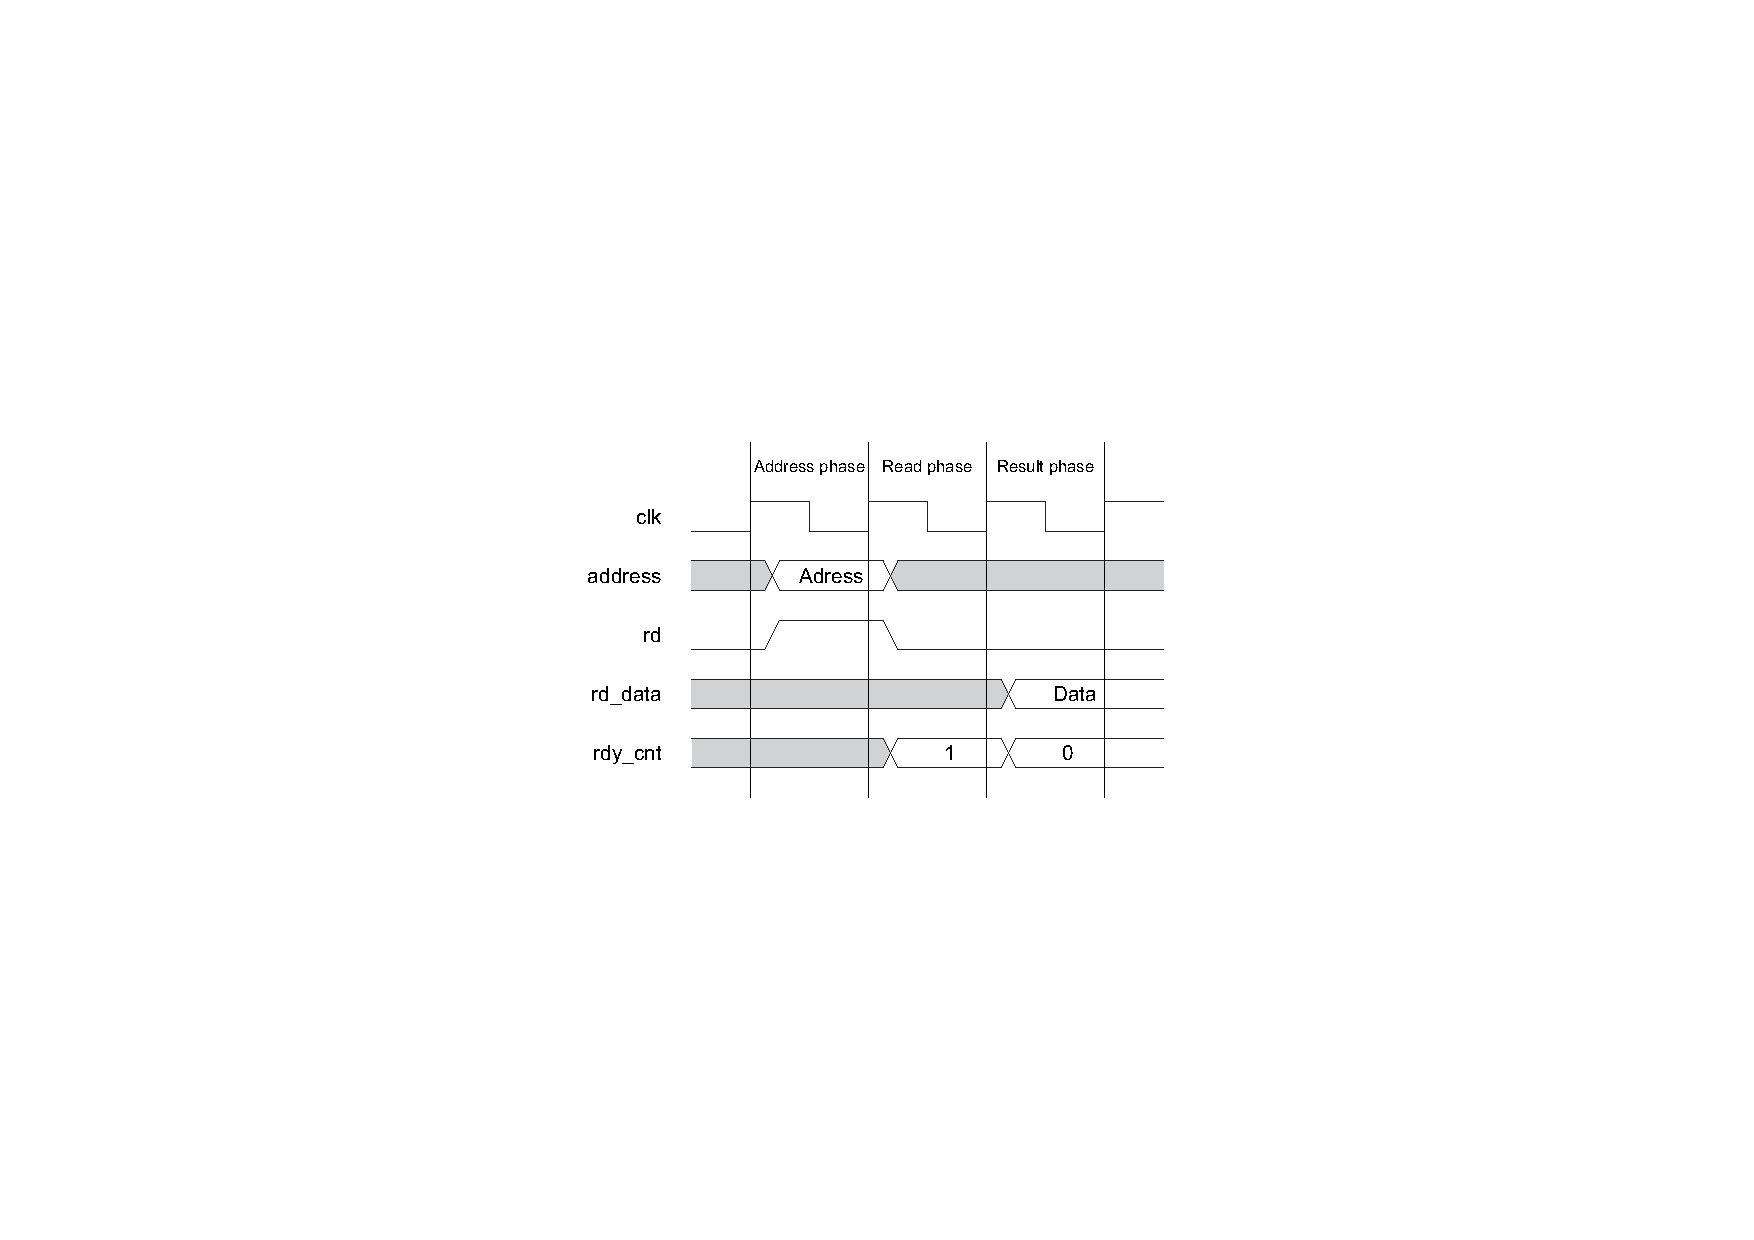
\includegraphics[scale=\scgrsc]{\scgrp/sc_basic_rd}
    \caption{Basic read transaction}
    \label{fig:sc:basic:rd}
\end{figure}

\subsection{Basic Write Transaction}

A write transaction consists of a single cycle address/command phase
started by assertion of \sign{wr} where the address and the write
data are valid. \sign{address} and \sign{wr\_data} are usually
registered by the slave. The end of the write cycle is signalled to
the master by the slave with \sign{rdy\_cnt}. See
Section~\ref{sec:ack} and an example in Figure~\ref{fig:sc:wr:ws}.

\section{SimpCon Signals}

This sections defines the signals used by the SimpCon connection.
Some of the signals are optional and may not be present on a
peripheral device.

All signals are a single direction point-to-point connection between
a master and a slave. The signal details are described by the device
that drives the signal. Table~\ref{tab:sc:signals} lists the signals
that define the SimpCon interface. The column Direction indicates
wether the signal is driven by the master or the slave.

\begin{table}
    \centering

    \begin{tabular}{lrlll}
        \toprule
        Signal & Width & Direction & Required & Description \\
        \midrule
        \sign{address} & 1--32 & Master & No & Address lines from the
        master\\
        & & & & to the slave port\\
        \sign{wr\_data} & 32 & Master & No & Data lines from the
        master\\
        & & & & to the slave port\\
        \sign{rd} & 1 & Master & No & Start of a read transaction \\
        \sign{wr} & 1 & Master & No & Start of a write transaction \\
        \sign{rd\_data} & 32 & Slave & No & Data lines from the
        slave\\
        & & & & to the master port\\
        \sign{rdy\_cnt} & 2 & Slave & Yes & Transaction end signalling \\
        \sign{rd\_pipeline\_level} & 2 & Slave & No & Maximum pipeline
        level\\
        & & & & for read transactions \\
        \sign{wr\_pipeline\_level} & 2 & Slave & No & Maximum pipeline
        level\\
        & & & & for write transactions \\
        \bottomrule

    \end{tabular}
    \caption{SimpCon port signals}
    \label{tab:sc:signals}

\end{table}



\subsection{Master Signal Details}

This section describes the signals that are driven by the master to
initiate a transaction.

\subsubsection{address}

Master addresses represent word addresses as offsets in the slaves
address range. \sign{address} is valid a single cycle either with
\sign{rd} for a read transaction or with \sign{wr} and
\sign{wr\_data} for a write transaction.

The number of bits for \sign{address} depend on the slaves address
range. For a single port slave \sign{address} can be omitted.

\subsubsection{wr\_data}

The \sign{wr\_data} signals carry the data for a write transaction.
It is valid for a single cycle together with \sign{address} and
\sign{wr}. The signal is typically 32 bits wide. Slaves can ignore
upper bits when the slave port is less than 32 bits.

\subsubsection{rd}

The \sign{rd} signal is asserted a single clock cycle to start a
read transaction. \sign{address} has to be valid in the same cycle.

\subsubsection{wr}

The \sign{wr} signal is asserted a single clock cycle to start a
write transaction. \sign{address} and \sign{wr\_data} have to be
valid in the same cycle.

\subsubsection{sel\_byte}

The \sign{sel\_byte} signal is reserved for future versions of the
SimpCon specification to add individual byte enables.

\subsection{Slave Signal Details}

This section describes the signals that are driven by the slave as a
response to transaction initiated by the master.

\subsubsection{rd\_data}

The \sign{wr\_data} signals carry the result for a read transaction.
The data is valid when \sign{rdy\_cnt} reaches 0 and stays valid
till a new read result is available. The signal is typically 32 bits
wide. Slaves that provide less than 32 bits should pad the upper
bits with 0.

\subsubsection{rdy\_cnt}

The \sign{rdy\_cnt} signal provides the number of cycles till the
pending transaction will finish. A 0 means that either read data is
available or a write transaction has been finished. Values of 1 and
2 mean the the transaction will finish in at least 1 or 2 cycles.
The maximum value is 3 and means the the transaction will finish in
3 or \emph{more} cycles. Note that not all values have to be used in
a transaction. Each monotonic sequence of \sign{rdy\_cnt} values is
legal.

\subsubsection{rd\_pipeline\_level}

The static \sign{rd\_pipeline\_level} provides the master with the
read pipeline level of the slave. The signal has to be constant to
enable the synthesizer to optimize the pipeline level dependent
state machine in the master.


\subsubsection{wr\_pipeline\_level}

The static \sign{wr\_pipeline\_level} provides the master with the
write pipeline level of the slave. The signal has to be constant to
enable the synthesizer to optimize the pipeline level dependent
state machine in the master.

\section{Slave Acknowledge}
\label{sec:ack}

Flow control between the slave and the master is usually done by a
single signal in the form of \emph{wait} or \emph{acknowledge}. The
\sign{ack} signal, e.g.\ in the Wishbone specification, is set when
the data is available or the write operation has finished. However,
for a pipelined master it can be of interest to know it
\emph{earlier} when a transaction will finish.


For many slaves, e.g.\ an SRAM interface with fixed wait states,
this information is available inside the slave. In the SimpCon
interface this information is communicated to the master through the
two bit ready counter (\sign{rdy\_cnt}). \sign{rdy\_cnt} signals the
number of cycles till the read data will be available or the write
transaction will be finished. Value 0 is equivalent to an \emph{ack}
signal and 1, 2, and 3 are equivalent to a wait request with the
distinction that the master knows how long the wait request will
last.

To avoid too many signals at the interconnect \sign{rdy\_cnt} has a
width of two bits. Therefore, the maximum value of 3 has the special
meaning that the transaction will finish in 3 or \emph{more} cycles.
As a result the master can only use the values 0, 1, and 2 to
release actions in its pipeline. If necessary an extension for a
longer pipeline is straightforward with a larger
\sign{rdy\_cnt}\footnote{The maximum value of the ready counter is
relevant for the early restart of a waiting master. A longer latency
from the slave e.g., for DDR SDRAM, will map to the maximum value of
the counter for the first cycles.}.

Idle slaves will keep the former value of 0 for \sign{rdy\_cnt}.
Slaves, that don't know in advance how many wait states are needed
for the transaction can produce sequences that omit any of the
numbers 3, 2, and 1. A simple slave can hold \sign{rdy\_cnt} on 3
until the data is available and set it than directly to 0. The
master has to handle those situations. Practically this reduces the
possibilities of pipelining and therefore the performance of the
interconnect. The master will read the data later, which is not an
issue as the data stays valid.

Figure~\ref{fig:sc:rd:ws} shows an example of a slave that needs
three cycles for the read to be processed. In cycle 1 the read
command and the address are set by the master. The slave registers
the address and sets \sign{rdy\_cnt} to 3 in cycle 2. The read takes
three cycles (2--4) during which \sign{rdy\_cnt} gets decremented.
In cycle 4 the data is available inside the slave and gets
registered. It is available in cycle 5 for the master and
\sign{rdy\_cnt} is finally 0. Both, the \sign{rd\_data} and
\sign{rdy\_cnt} will keep their value till a new transaction is
requested.

\begin{figure}
    \centering
    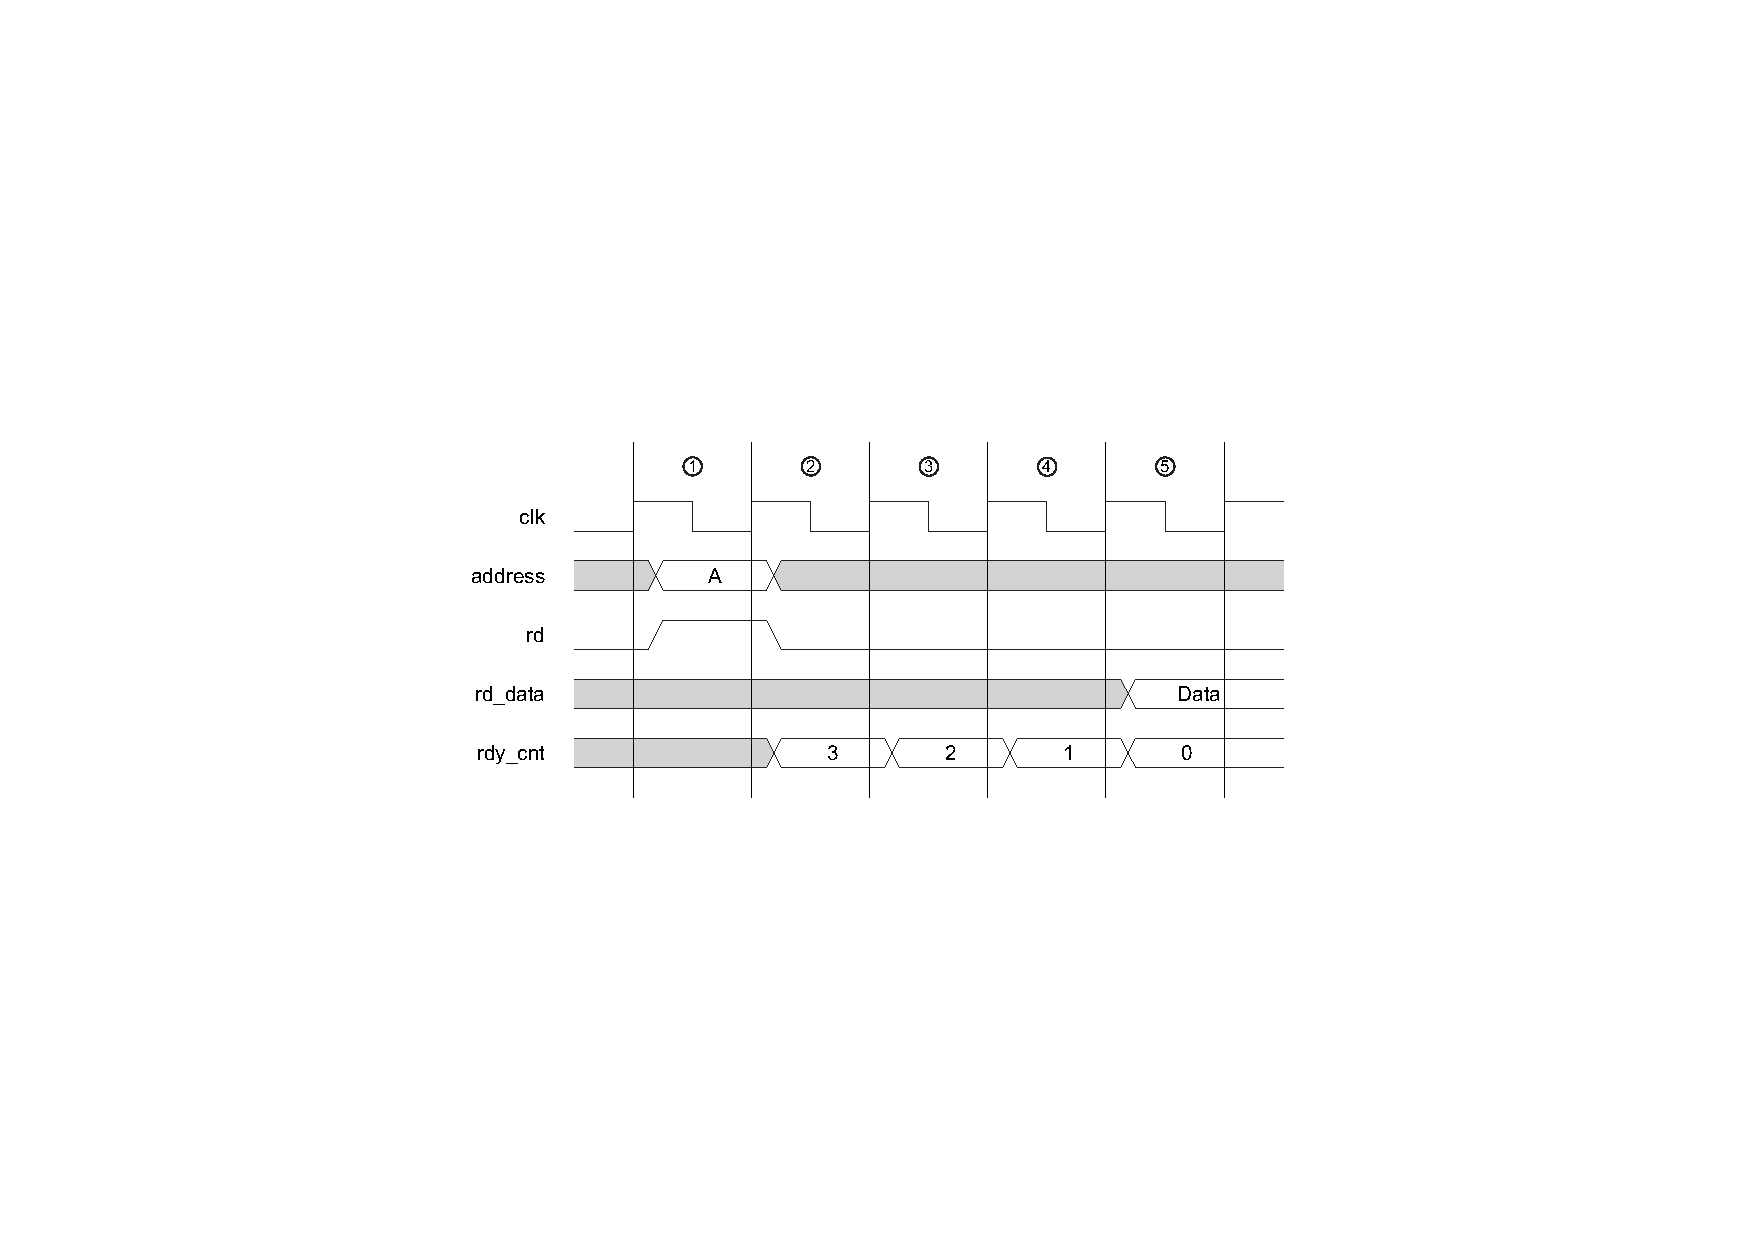
\includegraphics[scale=\scgrsc]{\scgrp/sc_rd_ws}
    \caption{Read transaction with wait states}
    \label{fig:sc:rd:ws}
\end{figure}


Figure~\ref{fig:sc:wr:ws} shows an example of a slave that needs
three cycles for the write to be processed. The address, the data to
be written and the write command are valid during cycle 1. The slave
registers the address and write data during cycle 1 and performs the
write operation during cycles 2--4. The \sign{rdy\_cnt} is
decremented and a non-pipelined slave can accept a new command after
cycle 4.

\begin{figure}
    \centering
    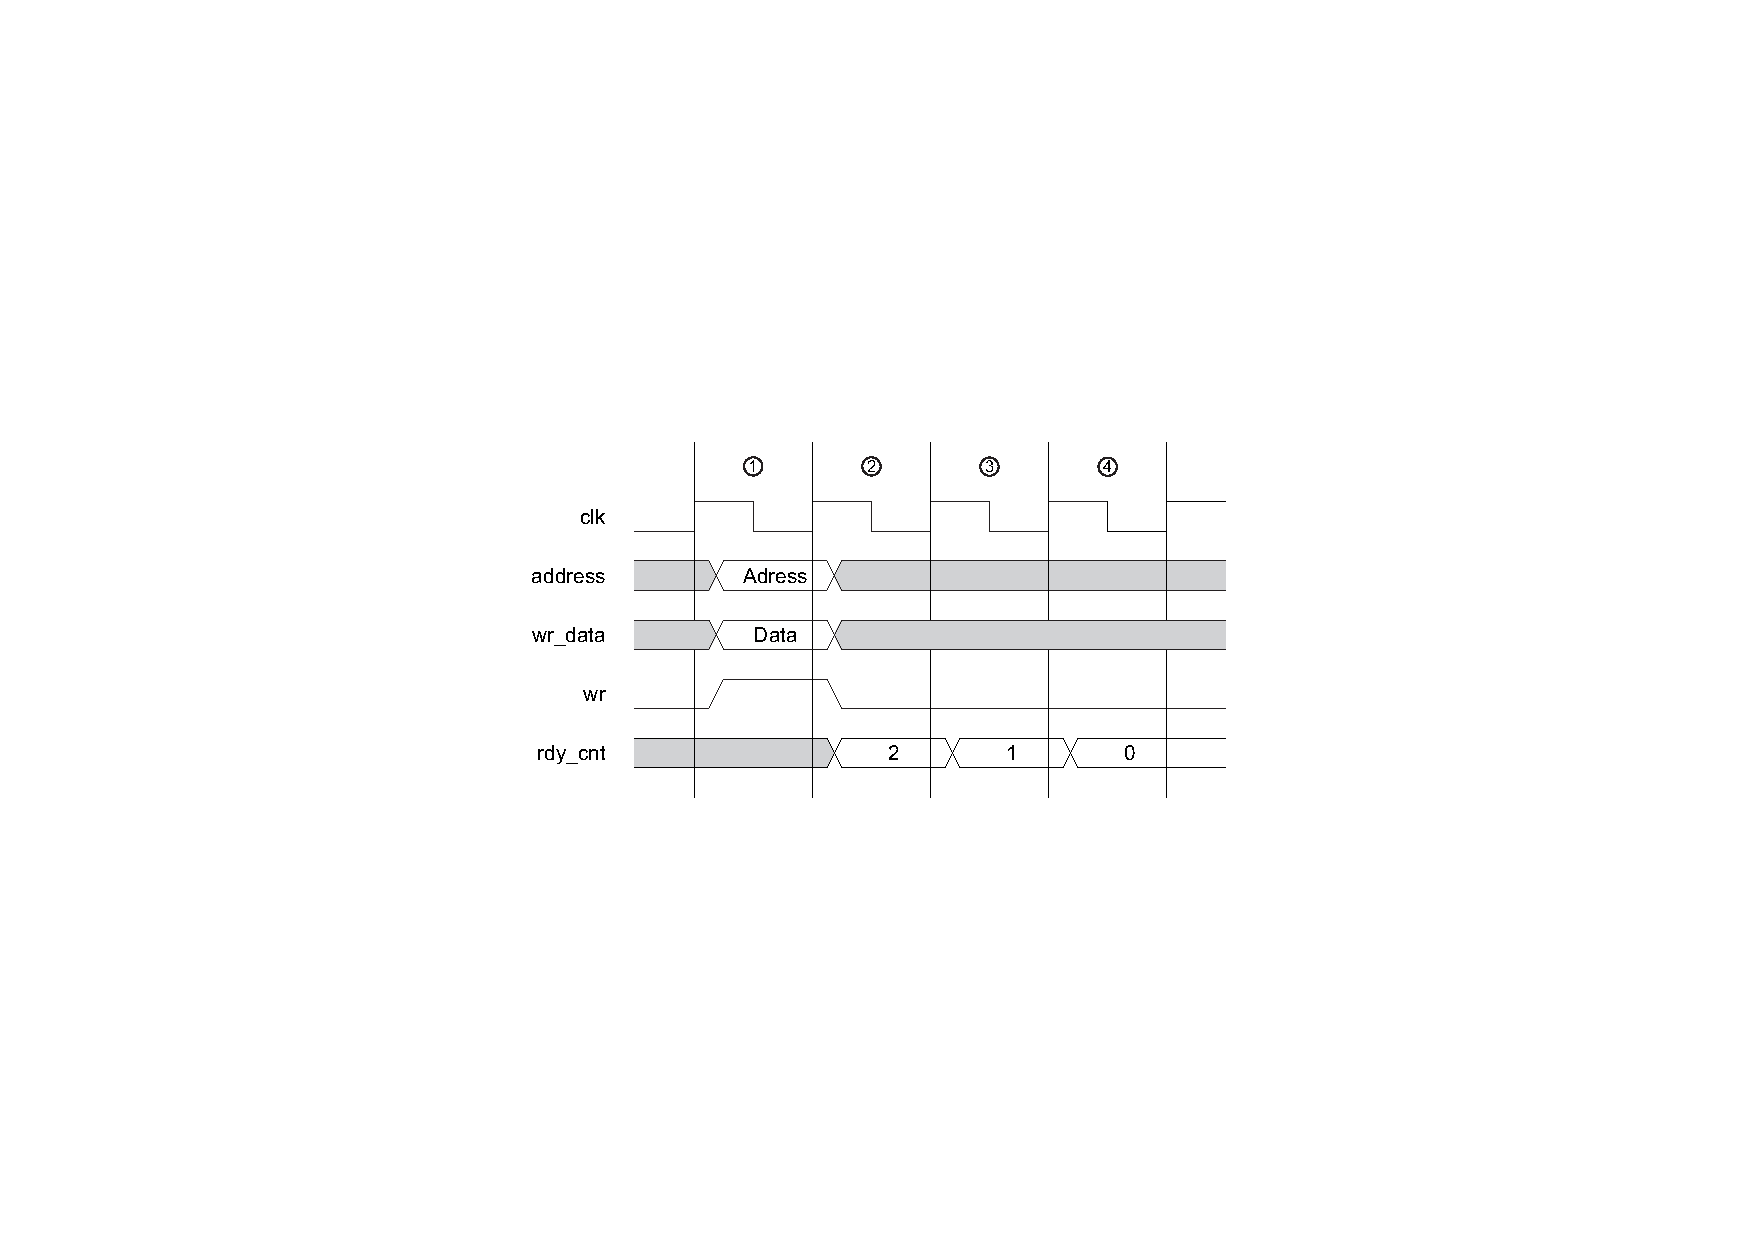
\includegraphics[scale=\scgrsc]{\scgrp/sc_wr_ws}
    \caption{Write transaction with wait states}
    \label{fig:sc:wr:ws}
\end{figure}



\section{Pipelining}

Figure~\ref{fig:sc:pipe:level} shows a read transaction for a slave
with four clock cycles latency. Without any pipelining the next read
transaction will start in cycle 7 after the data from the former
read transaction is read by the master. The three bottom lines show
when new read transactions (only the \sign{rd} signal is shown,
address lines are omitted from the figure) can be started for
different pipeline levels. With pipeline level 1 a new transaction
can start in the same cycle when the former read data is available
(in this example in cycle 6). At pipeline level 2 a new transaction
(either read or write) can start when \sign{rdy\_cnt} is 1, for
pipeline level 2 the next transaction can start at a \sign{rdy\_cnt}
of 2.

\begin{figure}
    \centering
    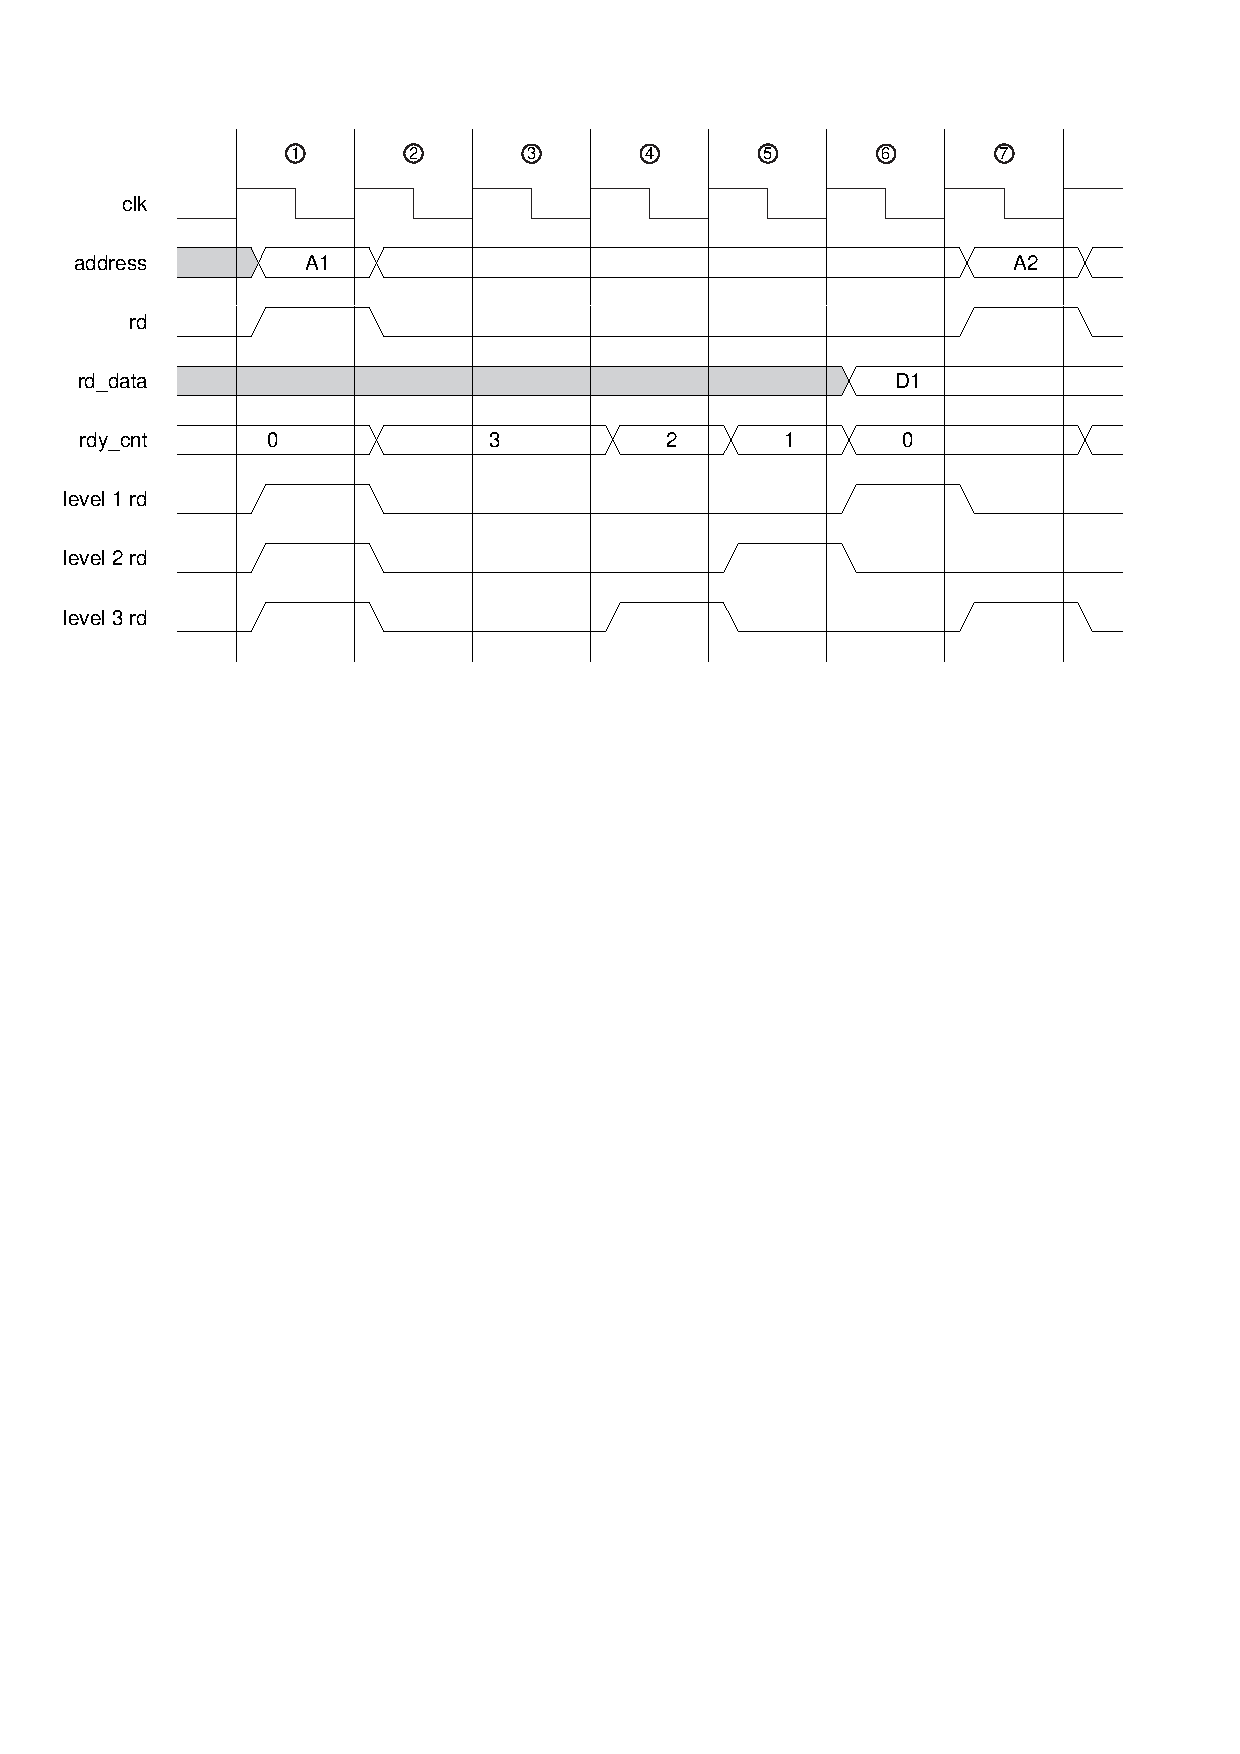
\includegraphics[scale=\scgrsc]{\scgrp/sc_pipe_level}
    \caption{Different pipeline levels for a read transaction}
    \label{fig:sc:pipe:level}
\end{figure}

The implementation of level 1 in the slave is trivial (just two more
transitions in the state machine). It is recommended to provide  at
least level 1 for read transactions. Level 2 is a little bit more
complex but usually no additional address or data registers are
necessary.

To implement level 3 pipelining in the slave at least an additional
address register is needed. However, to use level 3 the master has
to issue the request in the same cycle as \sign{rdy\_cnt} goes to 2.
That means this transition is combinatorial. We see in
Figure~\ref{fig:sc:pipe:level} that \sign{rdy\_cnt} value of 3 means
three or more cycles till the data is available and can therefore
not be used to trigger a new transaction. Extension to an even
deeper pipeline needs a wider \sign{rdy\_cnt}.


\subsection{Interconnect}

Although the definition of SimpCon is from a single master/slave
point-to-point viewpoint, all variations of multiple slave and
multiple master devices are possible.

\subsubsection{Slave Multiplexing}

To add several slaves to a single master \sign{rd\_data} and
\sign{rdy\_cnt} have to be multiplexed. Due to the fact that all
\sign{rd\_data} signals are already registered by the slaves a
single pipeline stage will be enough for a large multiplexer. The
selection of the multiplexer is also known at the transaction start
but needed at most in the next cycle. Therefore it can be registered
to further speed up the multiplexer.

%TODO: add a schematic for the master \sign{rd\_data} multiplexer.

\subsubsection{Master Multiplexing}

SimpCon defines no signals for the communication between a master
and an arbiter. However, it is possible to build a multi master
system with SimpCon. The SimpCon interface can be used as
interconnect between the masters and the arbiter and the arbiter and
the slaves. In this case the arbiter acts as slave for the master
and as master for the peripheral devices. An example of an arbiter
for SimpCon, where JOP and a VGA controller are two masters for a
shared main memory, can be found in \cite{jop:dma}. The same arbiter
is also used to build a chip-multiprocessor version of JOP.

The missing arbitration protocol in SimpCon results in the need to
queue $n-1$ requests in an arbiter for $n$ masters. However, this
additional hardware results in a zero cycle bus grant. The master,
which gets the bus granted, starts the slave transaction in the same
cycle as the original read/write request.

%TODO: add a timing diagram to explain this concept.


\section{Examples}

This section provides some examples for the application of the
SimpCon definition.

\subsection{IO Port}

TODO: Show how simple an IO port can be with SimpCon. We need no
addresses and can tie \sign{bsy\_cnt} to 0. We only need the
\sign{rd} or \sign{wr} signal to enable the port.

\subsection{SRAM interface}

The following example is taken from an implementation of SimpCon for
a Java processor. The processor is clocked with 100MHz and the main
memory consists of 15ns static RAMs. Therefore the minimum access
time for the RAM is two cycles. The slack time of 5ns forces us to
use output registers for the RAM address and write data and input
registers for the read data in the IO cells of the FPGA. These
registers fit nice with the intention of SimpCon to use registers
inside the slave.

Figure~\ref{fig:sc:sram} shows the memory interface for a
non-pipelined read access followed by a write access. Four signals
are driven by the master and two signals by the slave. The lower
half of the figure shows the signals at the FPGA pins where the RAM
is connected.


\begin{figure}
    \centering
    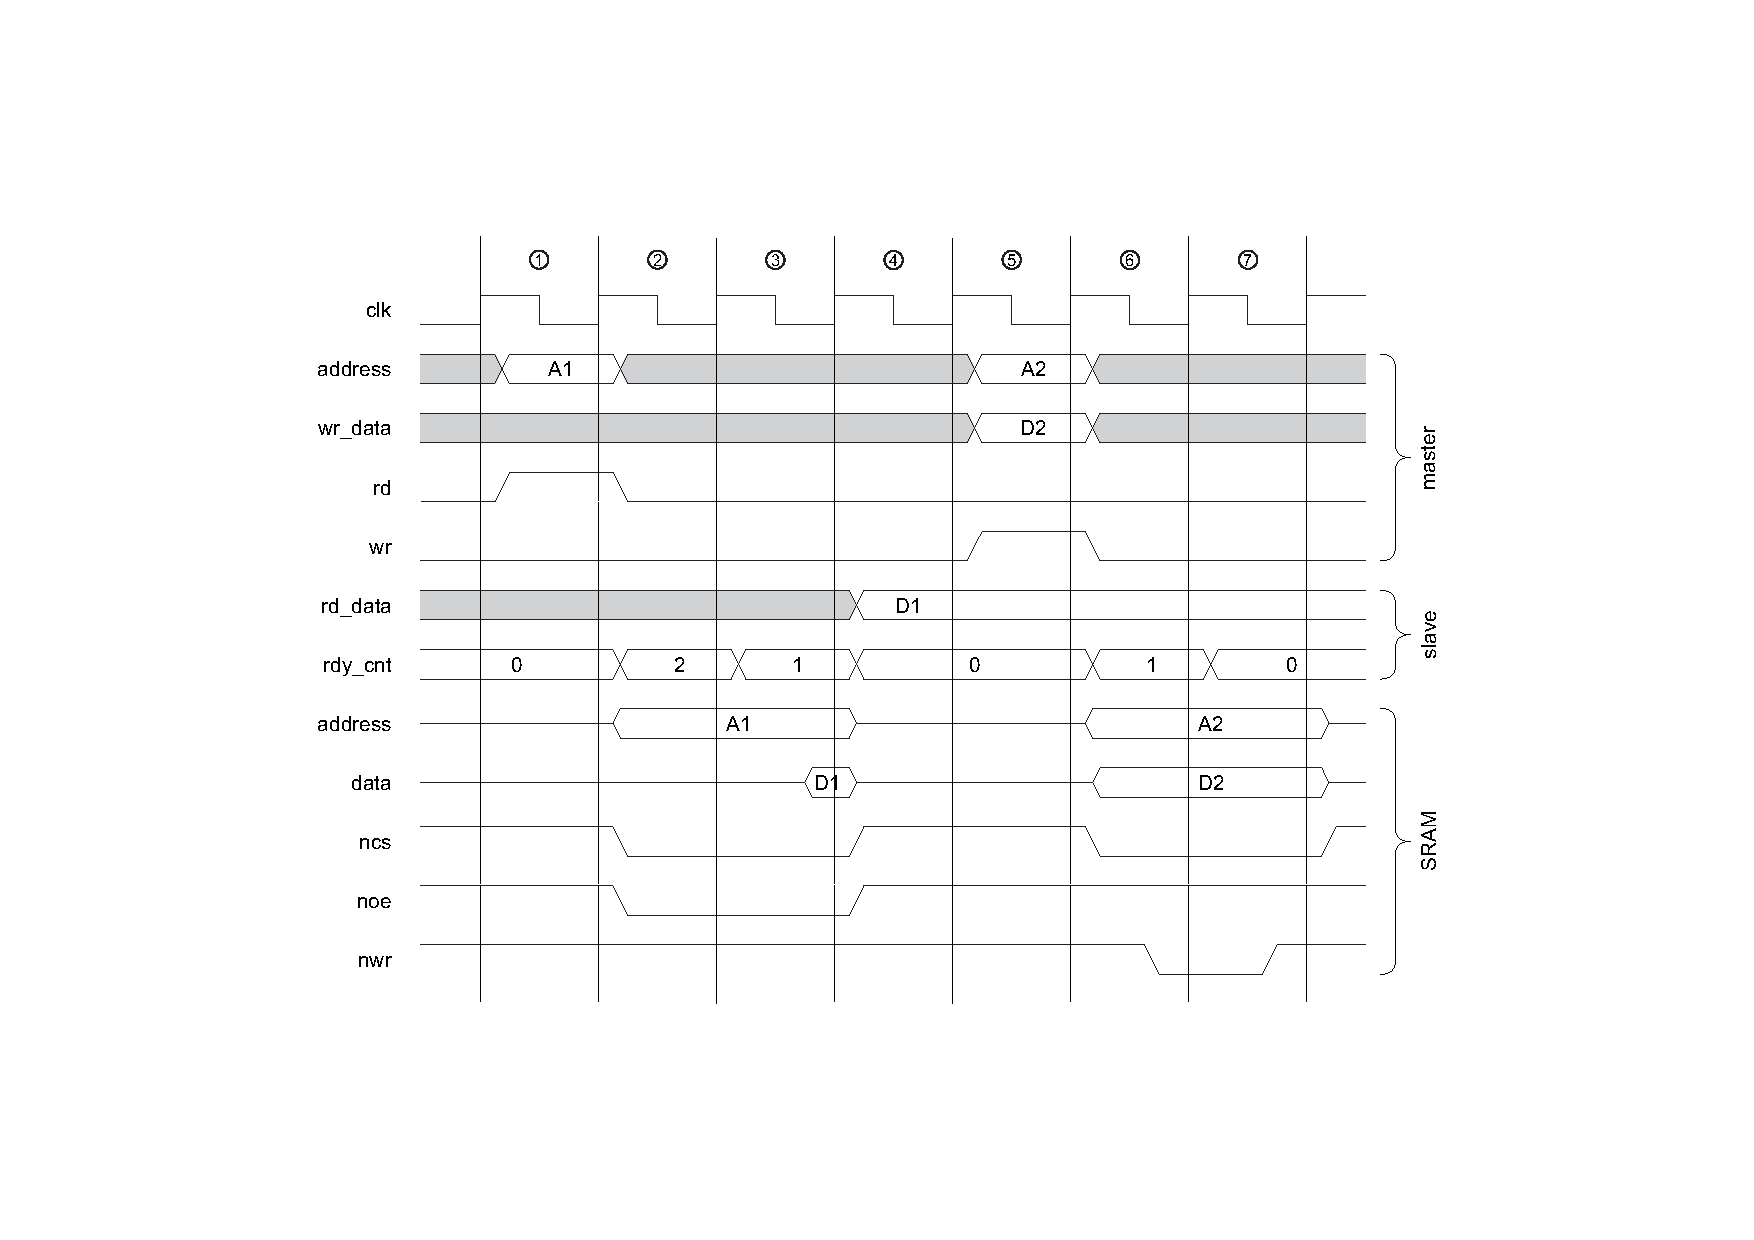
\includegraphics[scale=\scgrsc]{\scgrp/sc_sram}
    \caption{Static RAM interface without pipelining}
    \label{fig:sc:sram}
\end{figure}

In cycle~1 the read transaction is started by the master and the
slave registers the address. The slave also sets the registered
control signals \sign{ncs} and \sign{noe} during cycle~1. Due to the
placement of the registers in the IO cells, the address and control
signals are valid at the FPGA pins very early in cycle~2. At the end
of cycle~3 (15~ns after \sign{address}, \sign{ncs} and \sign{noe}
are stable) the data from the RAM is available and can be sampled
with the rising edge for cycle~4. The setup time for the read
register is short as the register can be placed in the IO cell. The
master reads the data in cycle~4 and starts a write transaction in
cycle~5. Address and data are again registered by the slave and are
available for the RAM at the beginning of cycle~6. To perform a
write in two cycles the \sign{nwr} signal is registered by a
negative triggered flip-flop.

In Figure~\ref{fig:sc:sram:prd} we see a pipelined read from the RAM
with pipeline level 2. With this pipeline level and the two cycles
read access time of the RAM we achieve the maximum possible
bandwidth.

\begin{figure}
    \centering
    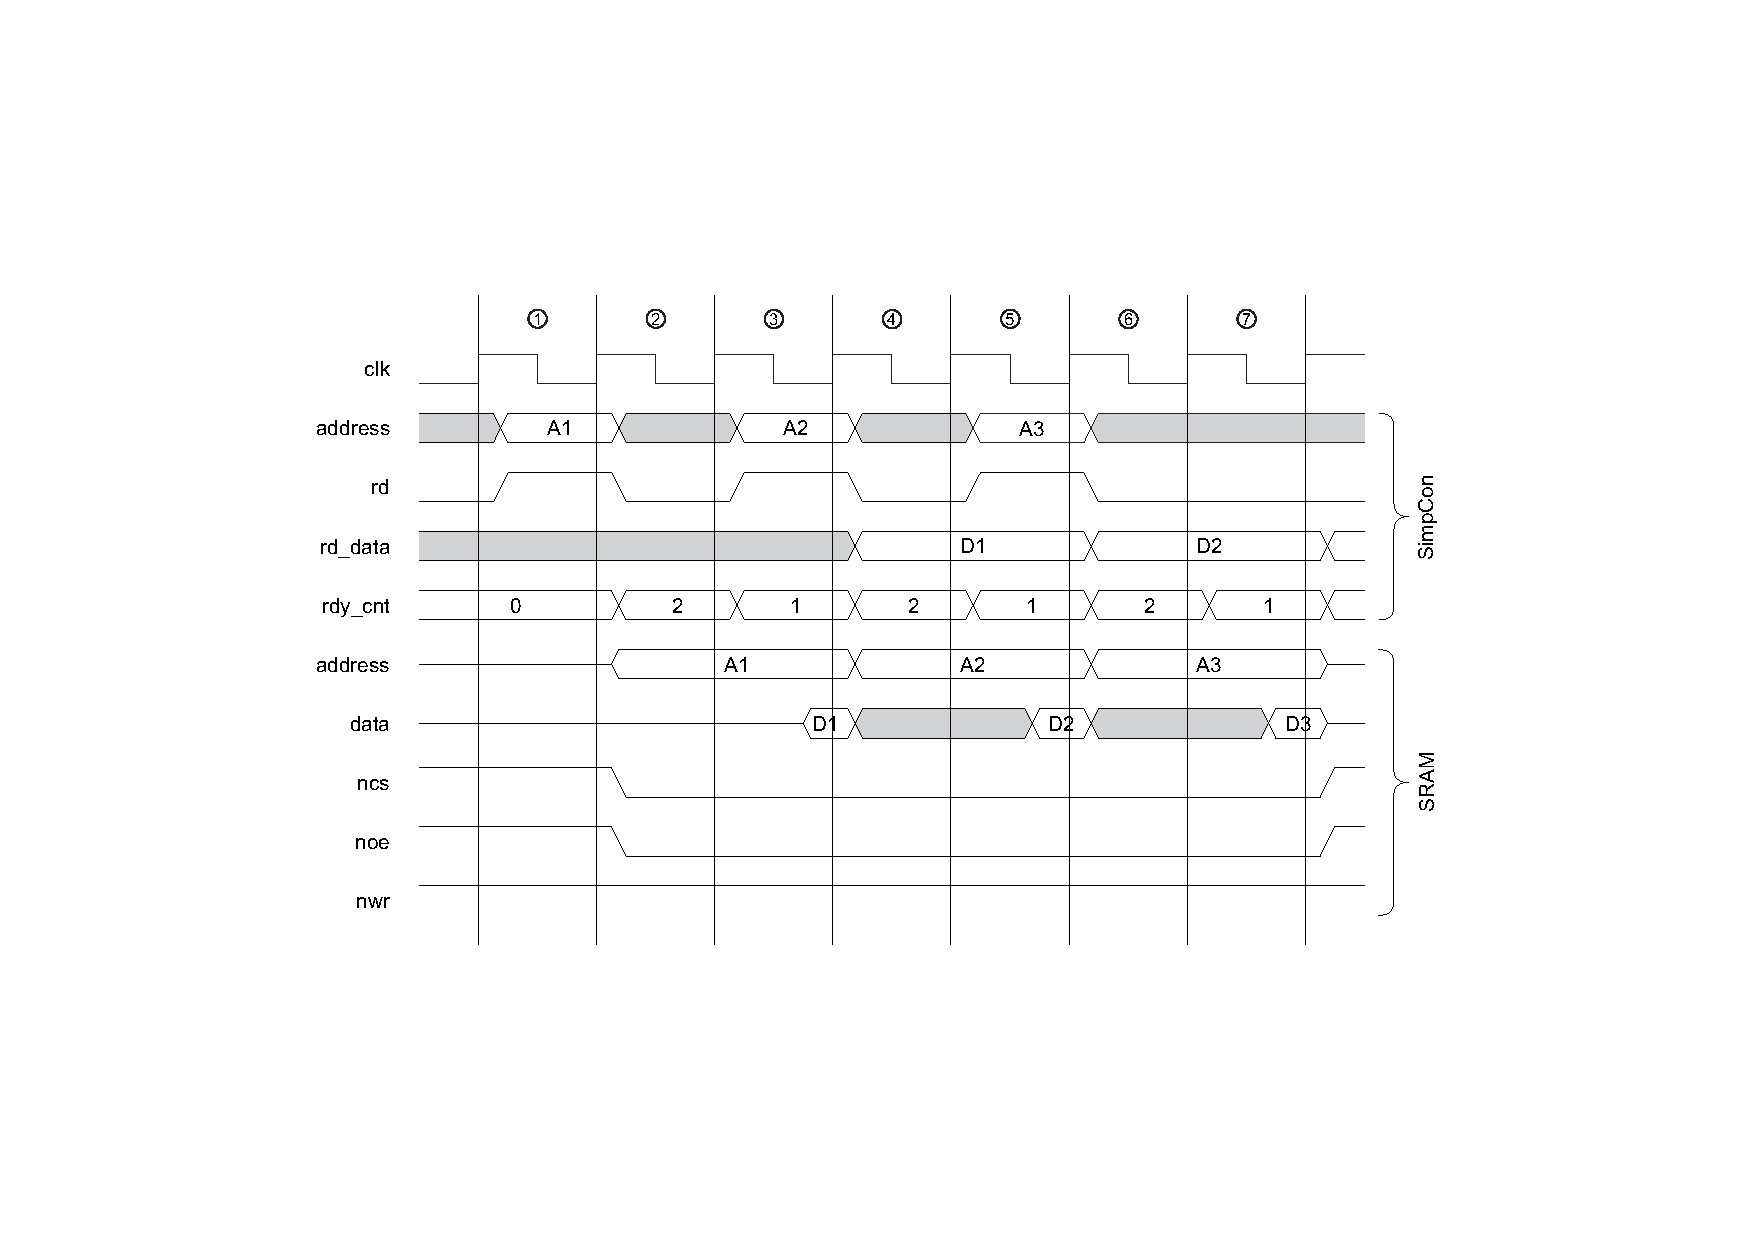
\includegraphics[scale=\scgrsc]{\scgrp/sc_sram_prd}
    \caption{Pipelined read from a static RAM}
    \label{fig:sc:sram:prd}
\end{figure}

We can see the start of the second read transaction in cycle 3
during the read of the first data from the RAM. The new address is
registered in the same cycle and available for the RAM in the
following cycle 4. Although we have a pipeline level of 2 we need no
additional address or data register. The read data is available for
two cycles (\sign{rdy\_cnt} 2 or 1 for the next read) and the master
is free to select one of the two cycles to read the data.

It has to be noted that pipelining with one read per cycle is
possible with SimpCon. We just showed a 2 cycle slave in this
example. For a SDRAM memory interface the ready counter will stay
either at 2 or 1 during the single cycle reads (depending on the
slave pipeline level). It will go down to 0 only for the last data
word to read.

\subsection{Master Multiplexing}

To add several slaves to a single master the \sign{rd\_data} and
\sign{bsy\_cnt} have to be multiplexed. Due to the fact that all
\sign{rd\_data} signals are registered by the slaves a single
pipeline stage will be enough for a large multiplexer. The selection
of the multiplexer is also known at the transaction start but needed
at most in the next cycle. Therefore it can be registered to further
speed up the multiplexer.
\ \\
\ \\
TODO: add a schematic for the master \sign{rd\_data} multiplexer.

\section{Available VHDL Files}

Besides the SimpCon documentation some example VHDL files for slave
devices and bridges are available from
\url{http://www.opencores.org/projects.cgi/web/simpcon/overview}.
All components are also part of the standard JOP distribution.


\subsection{Components}

\begin{itemize}
    \item \code{sc\_pack.vhd} defines VHDL records and some
    constants.
    \item \code{sc\_test\_slave} is a very simple SimpCon device. A
    counter to be read out and a register that can be written and
    read. There is no connection to the outer world. This example
    can be used as basis for a new SimpCon device.
    \item \code{sc\_sram16.vhd} is a memory controller for 16-bit
    SRAM.
    \item \code{sc\_sram32.vhd} is a memory controller for 32-bit
    SRAM.
    \item \code{sc\_sram32\_flash.vhd} is a memory controller for 32-bit
    SRAM, a NOR Flash, and a NAND Flash as used in the Cycore FPGA board for JOP.
    \item \code{sc\_uart.vhd} is a simple UART with configurable
    baud rate and FIFO width.
    \item \code{sc\_usb.vhd} is an interface to the parallel port of
    the FTDI 2232 USB chip. The register definition is identical to
    the UART and the USB connection can be used as a drop in
    replacement for a UART.
    \item \code{sc\_isa.vhd} interfaces the old ISA bus. It can be used
    for the popular CS8900 Ethernet chip.
    \item \code{sc\_sigdel.vhd} is a configurable sigma-delta converter
    for an FPGA that needs at minimum just two external components:
    a capacitor and a resistor.
    \item \code{sc\_fpu.vhd} provides an interface to the 32-bit FPU available
    at \url{www.opencores.org}.
    \item \code{sc\_arbiter.vhd} is a zero cycle latency, priority
    based SimpCon arbiter written by Christof Pitter \cite{jop:cmp}.
\end{itemize}

\subsection{Bridges}

\begin{itemize}
    \item \code{sc2wb.vhd} is a SimpCon/Wishbone \cite{soc:wishbone}
    bridge.
    \item \code{sc2avalon.vhd} is a SimpCon/Avalon \cite{soc:avalon}
    bridge to integrate a SimpCon based design with Altera's SOPC
    Builder \cite{quartus}.
    \item \code{sc2ahbsl.vhd} provides an interface to AHB slaves as
    defined in Gaisler's GRLIB \cite{grlib}. Many of the available
    GPL AHB modules from the GRLIB can be used in a SimpCon based
    design.
\end{itemize}


\section{Why a New Interconnection Standard?}

There are many interconnection standards available for SoC designs.
The natural question is: Why propose a new one? The answer is given
in the following section. For short: The available standards are
still in the tradition of backplane busses and do not fit very well
for pipelined on-chip interconnections.

\subsection{Common SoC Interconnections}


Several point-to-point and bus standards have been proposed over the
last years. The following section gives a brief overview of common
SoC interconnection standards.

The Advanced Microcontroller Bus Architecture (AMBA) \cite{soc:amba}
is the interconnection definition from ARM. The specification
defines three different busses: Advanced High-performance Bus (AHB),
Advanced System Bus (ASB), and Advanced Peripheral Bus (APB). The
AHB is used to connect on-chip memory, cache, and external memory to
the processor. Peripheral devices are connected to the APB. A bridge
connects the AHB to the lower bandwidth APB. An AHB bus transfer can
be one cycle with burst operation. With the APB a bus transfer
requires two cycles and no burst mode is available. Peripheral bus
cycles with wait states are added in the version 3 of the APB
specification. ASB is the predecessor of AHB and is not recommended
for new designs (ASB uses both clock phases for the bus signals --
very uncommon for today's synchronous designs). The AMBA 3 AXI
(Advanced eXtensible Interface) \cite{soc:amba3} is the latest
extension to AMBA. AXI introduces out-of-order transaction
completion with the help of a 4 bit transaction id tag. A ready
signal acknowledges the transaction start. The master has to hold
the transaction information (e.g.\ address) till the interconnect
signals ready. This enhancement ruins the elegant single cycle
address phase from the original AHB specification.

Wishbone \cite{soc:wishbone} is a public domain standard used by
several open-source IP cores. The Wishbone interface specification
is still in the tradition of microcomputer or backplane busses.
However, for a SoC interconnect, which is usually
point-to-point\footnote{Multiplexers are used instead of busses to
connect several slaves and masters.}, this is not the best approach.
The master is requested to hold the address and data valid through
the whole read or write cycle. This complicates the connection to a
master that has the data valid only for one cycle. In this case the
address and data have to be registered \emph{before} the Wishbone
connect or an expensive (time and resources) multiplexer has to be
used. A register results in one additional cycle latency. A better
approach would be to register the address and data in the slave. In
that case the address decoding in the slave can be performed in the
same cycle as the address is registered. A similar issue, with
respect to the master, exists for the output data from the slave: As
it is only valid for a single cycle the data has to be registered by
the master when the master is not reading it immediately. Therefore,
the slave should keep the last valid data at its output even when
the Wishbone strobe signal (\emph{wb.stb}) is not assigned anymore.
Holding the data in the slave is usually \emph{for free} from the
hardware complexity -- it is \emph{just} a specification issue. In
the Wishbone specification there is no way to perform pipelined read
or write. However, for blocked memory transfers (e.g. cache load)
this is the usual way to achieve good performance.


The Avalon \cite{soc:avalon} interface specification is provided by
Altera for a system-on-a-programmable-chip (SOPC) interconnection.
Avalon defines a great range of interconnection devices ranging from
a simple asynchronous interface intended for direct static RAM
connection up to sophisticated pipeline transfers with variable
latencies. This great flexibility provides an easy path to connect a
peripheral device to Avalon. How is this flexibility possible? The
\emph{Avalon Switch Fabric} translates between all those different
interconnection types. The switch fabric is generated by Altera's
SOPC Builder tool. However, it seems that this switch fabric is
Altera proprietary thus tying this specification to Altera FPGAs.

The On-Chip Peripheral Bus (OPB) \cite{soc:opb} is an open standard
provided by IBM and used by Xilinx. The OPB specifies a bus for
multiple masters and slaves. The implementation of the bus is not
directly defined in the specification. A distributed ring, a
centralized multiplexer, or a centralized AND/OR network are
suggested. Xilinx uses the AND/OR approach and all masters and
slaves must drive the data busses to zero when inactive.


Sonics Inc. defined the Open Core Protocol (OCP) \cite{soc:ocp} as
an open, freely available standard. The standard is now handled by
the OCP International Partnership\footnote{\url{www.ocpip.org}}.




\subsection{What's Wrong with the Classic Standards?}

All SoC interconnection standards, that are widely in use, are still
in the tradition of a backplane bus. They force the master to hold
the address and control signals till the slave provides the data or
acknowledges the write request. However, this is not necessary in a
clocked, synchronous system. Why should we force the master to hold
the signals? Let the master move on after submitting the request in
a single cycle. Forcing the address and control valid for the
complete request disables any form of pipelined requests.


\begin{figure}
    \centering
    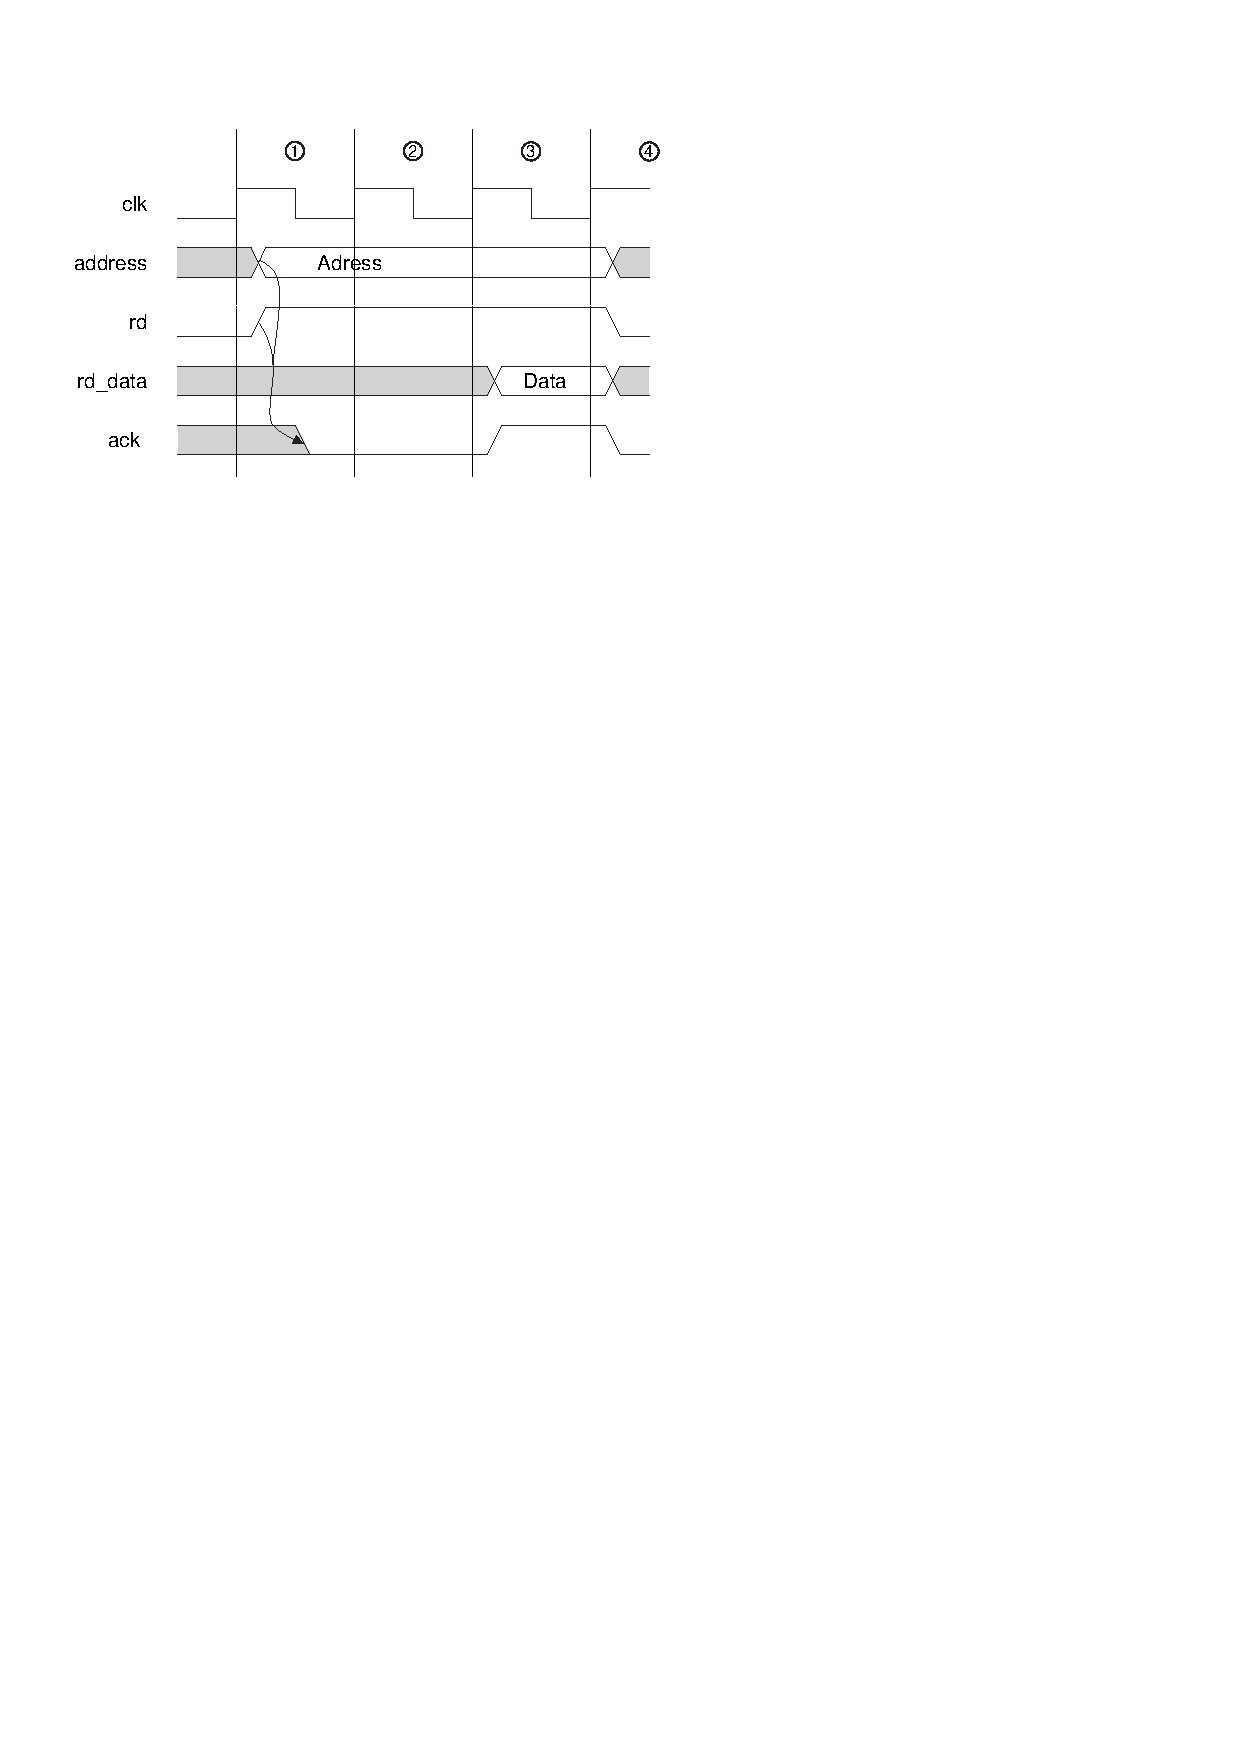
\includegraphics[scale=\scgrsc]{\scgrp/wb_basic_rd}
    \caption{Classic basic read transaction}
    \label{fig:wb:basic:rd}
\end{figure}

Figure~\ref{fig:wb:basic:rd} shows a read transaction with wait
states as defined in Wishbone \cite{soc:wishbone}, Avalon
\cite{soc:avalon}, OPB \cite{soc:opb}, and OCP
\cite{soc:ocp}\footnote{The signal names are different, but the
principle is the same for all mentioned busses.}. The master issues
the read request and the address in cycle 1. The slave has to reset
the \sign{ack} in the same cycle. When the slave data is available
the acknowledge signal is set (\sign{ack} in cycle 3). The master
has to read the data and register them within the same clock cycle.
The master has to hold the address, write data and control signal
active till the acknowledgement from the slave. For pipelined read
the \sign{ack} signal can be split into two signals (available in
Avalon and OCP): one to accept the request and a second one to
signal the available data.

The master is blind about the status of the outstanding transaction
until it is finished. It could be possible that the slave informs
the master in how many cycles the result will be available. This
information can help in building deeper pipelined masters.

Only the AMBA AHB \cite{soc:amba} defines a different protocol. A
single cycle address phase followed by a variable length data phase.
The slave acknowledgement (HREADY) is only necessary in the data
phase avoiding the combinatorial path from address/command to the
acknowledgement. Overlapping address and data phase is allowed and
recommended for high performance. Compared to SimpCon, AMBA AHB
allows for single stage pipelining, whereas SimpCon makes
multi-stage pipelining possible using the ready counter
(\sign{rdy\_cnt}). The \sign{rdy\_cnt} signal defines the delay
between the address and the data on a read, signalled by the slave.
Therefor, the pipeline depth of the bus and the slaves is only
limited by the bit width of \sign{rdy\_cnt}.


Another issue with all interconnection standards is the single cycle
availability of read data at the slaves. Why not keep the read data
valid as long as there is no new read data available? This feature
would allow the master to be more flexible when to read the data. It
would allow to issue a read command and then continue with other
instructions -- a feature known as data pre-fetching to hide long
latencies.

The last argument sounds contradictory to the first argument on
providing the transaction data at the master just for a single
cycle, but requesting the slave to hold the data for several cycles.
However, it is motivated to free up the master, keep it
\emph{moving}, and move the data hold (register) burden into the
slave. As data processing bottlenecks are usually found in the
master devices it sounds natural to move as much work as possible to
the slave devices to free up the master.

Avalon, Wishbone and OPB provide a single cycle latency access to
slaves due to the possibility to acknowledge a request in the same
cycle. However, this feature is a scaling issue for larger systems.
There is a combinatorial path from master address/command to address
decoding, slave decision on \sign{ack}, slave \sign{ack}
multiplexing back to the master and the master decision to hold
address/command or read the data and continue. Also the slave output
data multiplexer is on a combinatorial path from the master address.

AMBA AHB and SimpCon avoid this scaling issue by requesting the
acknowledge in the cycle following the command. In SimpCon and AMBA
the select for the read data multiplexer can be registered as the
read address is known at least one cycle before the data is
available. The later acknowledge results in a minor drawback on
SimpCon and AMBA (nothing is for free): It is not possible to
perform a single cycle read or write without pipelining. A single,
non pipelined transaction takes two cycles without a wait state.
However, a single cycle read transaction is only possible for very
simple slaves. Most non-trivial slaves (e.g.\ memory interfaces)
will not allow a single cycle access anyway.

\subsection{Evaluation}

We compare the SimpCon interface with the AMBA and the Avalon
interface as two examples of common interconnection standards. As
evaluation example we interface an external asynchronous SRAM with a
tight timing. The system is clocked with 100 MHz and the access time
for the SRAM is 15 ns. Therefore, there are 5 ns available for
on-chip register to SRAM input and SRAM output to on-chip register
delays. As SoC we use an actual low-cost FPGA (Cyclone EP1C6
\cite{AltCyc} and a Cyclone II).

The master is a Java processor (JOP \cite{jop:thesis,
jop:jnl:jsa2007}). The processor is configured with 4~KB instruction
cache and 512 Byte on-chip stack cache. We run a complete
application benchmark on the different systems. The embedded
benchmark (\emph{Kfl} as described in \cite{jop:austrochip05}) is an
industrial control application already in production.


%For a different benchmark (a UDP/IP application with IP processing -
%lot of buffer access) the difference is larger.

\begin{table}
    \centering

    \begin{tabular}{rll}
        \toprule
        Performance &      Memory     & Interconnect \\
        \midrule
        16,633 &  32 bit SRAM & SimpCon \\

        14,259 &  32 bit SRAM & AMBA \\

        14,015 &  32 bit SRAM & Avalon/PTF \\
        13,920 &  32 bit SRAM & Avalon/VHDL \\
        15,762 & 32 bit on-chip & Avalon\\

        14,760 &  16 bit SRAM & SimpCon \\

        11,322 &  16 bit SRAM & Avalon \\


         7,288  & 16 bit SDRAM & Avalon \\


%        Kfl & UDP/IP   &  Memory     & Interconnect \\
%        \midrule
%        16,633 & 6,537 & 32 bit SRAM & SimpCon \\
%
%        14,015 &       & 32 bit SRAM & Avalon/PTF \\
%        13,920 &       & 32 bit SRAM & Avalon/VHDL \\
%
%        14,760 & 5,716 & 16 bit SRAM & SimpCon \\
%
%        11,322 & 4,302 & 16 bit SRAM & Avalon \\
%        15,762 & --    & 32 bit on-chip & Avalon\\
%
%
%         7,288 & 2,677 & 16 bit SDRAM & Avalon \\


        \bottomrule

    \end{tabular}
    \caption{JOP performance with different interconnection types}
    \label{tab:perf:diff}

%         5,630 & 2,140 &  50 MHz & 16 bit SRAM (relaxed timing) & Avalon \\
%         6,243 & 2,389 &  50 MHz & 16 bit SRAM & Avalon \\

\end{table}

Table~\ref{tab:perf:diff} shows the performance numbers of this
JOP/SRAM interface on the embedded benchmark. It measures
iterations/s and therefore higher numbers are better. One iteration
is the execution of the main control loop of the \emph{Kfl}
application. For a 32 bit SRAM interface we compare SimpCon against
AMBA and Avalon. SimpCon outperforms AMBA by 17\% and Avalon by
19\%\footnote{The performance is the measurement of the execution
time of the whole application, not only the difference between the
bus transactions.} on a 32 bit SRAM.

The AMBA experiment uses the SRAM controller provided as part of
GRLIB \cite{grlib} by Gaisler Research. We avoided writing our own
AMBA slave to verify that the AMBA implementation on JOP is correct.
To provide a fair comparison between the single master solutions
with SimpCon and Avalon the AMBA bus was configured without an
arbiter. JOP is connected directly to the AMBA memory slave. The
difference between the SimpCon and the AMBA performance can be
explained by two facts: (1) as with the Avalon interconnect, the
master has the information when the slave request is ready at the
same cycle when the data is available (compared to the
\sign{rdy\_cnt} feature); (2) the SRAM controller is conservative as
it asserts \sign{HREADY} one cycle later than the data is available
in the read register (\sign{HRDATA}). The second issue can be
overcome by a better implementation of the SRAM AMBA slave.


The Avalon experiment considers two versions: an SOPC Builder
generated interface (PTF) to the memory and a memory interface
written in VHDL. The SOPC Builder interface performs slightly better
than the VHDL version that generates the Avalon \sign{waitrequest}
signal. It is assumed that the SOPC Builder version uses fixed wait
states within the switch fabric.

We also implemented an Avalon interface to the single-cycle on-chip
memory. SimpCon is even faster with the 32 bit off-chip SRAM than
with the on-chip memory connected via Avalon. Furthermore, we also
performed experiments with a 16 bit memory interface to the same
SRAM. With this smaller data width the pressure on the
interconnection and memory interface is higher. As a result the
difference between SimpCon and Avalon gets larger (30\%) on the 16
bit SRAM interface. To complete the picture we also measured the
performance with an SDRAM memory connected to the Avalon bus. We see
that the large latency of an SDRAM is a big performance issue for
the Java processor.

\section{Summary}

This document describes a simple (with respect to the definition and
implementation) and efficient SoC interconnect. The novel signal
\sign{rdy\_cnt} allows an early signalling to the master when read
data will be valid. This feature allows the master to restart a
stalled pipeline earlier to react for arriving data. Furthermore,
this feature also enables pipelined bus transactions with a minimal
effort on the master and the slave side.

We have compared SimpCon quantitative with AMBA and Avalon, two
common interconnection definitions. The application benchmark shows
a performance advantage of SimpCon by 17\% over AMBA and 19\% over
Avalon interfaces to an SRAM.

SimpCon is used as the main interconnect for the Java processor JOP
in a single master, multiple salves configuration. SimpCon is also
used to implement a shared memory chip-multiprocessor version of
JOP. Furthermore, in a research project on time-triggered
network-on-chip \cite{jop:ttnoc} SimpCon is used as the
\emph{socket} to this NoC.

The author thanks Kevin Jennings and Tommy Thorn for the interesting
discussions about SimpCon, Avalon and on-chip interconnection in
general at the usenet newsgroup \texttt{comp.arch.fpga}.


\chapter{Chip Multiprocessing}
\label{chap:cmp}
\index{CMP}

This chapter describes the configuration of a chip multiprocessor
(CMP) version of JOP. The various SimpCon based arbiters have been
developed by Christof Pitter and are described in \cite{jop:dma,
jop:cmp, jop:cmp:eval}.

The project file to start with is \code{cyccmp}, a configuration for
three processors with a TDMA based arbiter in the Cycore board with
the EP1C12.

\section{Booting a CMP System}

\index{CMP!booting}

One interesting issue for a CMP system is the question how the
startup or boot-up is performed. Before we explain the CMP solution,
we need an understanding of the boot-up sequence of JOP in an FPGA.
On power-up, the FPGA starts the configuration state machine to read
the FPGA configuration data either from a Flash or via a download
cable (for development). When the configuration has finished an
internal reset is generated. After that reset, microcode instructions
are executed starting from address 0. At this stage, we have not yet
loaded any application program (Java bytecode). The first sequence in
microcode performs this task. The Java application can be loaded from
an external Flash or via a serial line (or USB port) from a PC. The
microcode assembly configured the mode. Consequently, the Java
application is loaded into the main memory. To simplify the startup
code we perform the rest of the startup in Java itself, even when
some parts of the JVM are not yet setup.

In the next step, a minimal stack frame is generated and the special
method \code{Startup.boot()} is invoked. From now on JOP runs in Java
mode. The method \code{boot()} performs the following steps:
\begin{samepage}
\begin{itemize}
    \item Send a greeting message to \emph{stdout}
    \item Detect the size of the main memory
    \item Initialize the data structures for the garbage
        collector
    \item Initialize \code{java.lang.System}
    \item Print out JOP's version number, detected clock speed,
        and memory size
    \item Invoke the static class initializers in a predefined
        order
    \item Invoke the \code{main} method of the application class
\end{itemize}
\end{samepage}

The boot-up process is the same for all processors until the
generation of the internal reset and the execution of the first
microcode instruction. From that point on, we have to take care that
\emph{only one} processor performs the initialization steps.

All processors in the CMP are functionally identical. Only one
processor is designated to boot-up and initialize the whole system.
Therefore, it is necessary to distinguish between the different CPUs.
We assign a unique CPU identity number (CPU ID) to each processor.
Only processor CPU0 is designated to do all the boot-up and
initialization work. The other CPUs have to wait until CPU0 completes
the boot-up and initialization sequence. At the beginning of the
booting sequence, CPU0 loads the Java application. Meanwhile, all
other processors are waiting for an \emph{initialization finished}
signal of CPU0. This busy wait is performed in microcode. When the
other CPUs are enabled, they will run the same sequence as CPU0.
Therefore, the initialization steps are guarded by a condition on the
CPU ID.

In our current prototype, we let all additional CPUs also invoke the
main method of the application. This is a shortcut for a simple
evaluation of the system\footnote{In the main method we execute
different applications based on the CPU ID.}. In a future version,
the additional CPUs will invoke a system method to be integrated into
the normal scheduling system.


\section{CMP Scheduling}

\index{CMP!scheduling}

There are two possibilities to run multiple threads on the CMP
system:

\begin{enumerate}
  \item A single thread per processor
  \item Several threads on each processor
\end{enumerate}

For the configuration of one thread per processor the scheduler does
not need to be started. Running several threads on each core is
managed via the JOP real-time threads \code{RtThread}. On each core a
local preemptive, priority based scheduler runs. Threads cannot
migrate from one core to another one.

\subsection{One Thread per Core}


The first processor executes, as usual, \code{main()}. To execute
code on the other cores a \code{Runnable} has to be registered for
each core. After registering those Runnables the other cores need to
be started. The following code shows an example that can be found in
\dirent{test/cmp/HelloCMP.java}.

\begin{verbatim}
public class HelloCMP implements Runnable {

    int id;

    static Vector msg;

    public HelloCMP(int i) {
        id = i;
    }

    /**
     * @param args
     */
    public static void main(String[] args) {

        msg = new Vector();

        System.out.println("Hello World from CPU 0");

        SysDevice sys = IOFactory.getFactory().getSysDevice();
        for (int i=0; i<sys.nrCpu-1; ++i) {
            Runnable r = new HelloCMP(i+1);
            Startup.setRunnable(r, i);
        }

        // start the other CPUs
        sys.signal = 1;

        // print their messages
        for (;;) {
            int size = msg.size();
            if (size!=0) {
                StringBuffer sb = (StringBuffer) msg.remove(0);
                System.out.println(sb);
            }
        }
    }

    public void run() {

        StringBuffer sb = new StringBuffer();
        sb.append("Hello World from CPU ");
        sb.append(id);
        msg.addElement(sb);
    }

}
\end{verbatim}

\subsection{Scheduling on the CMP System}

Running several threads on each core is possible with \code{RtThread}
and setting the core for each thread with
\code{RtThread.setProcessor(nr)}. The following example
(\code{test/cmp/RtHelloCMP.java}) shows registering 50 threads on
three cores. On \code{missionStart()} the threads are distributed to
the cores, a scheduler for each core registered as timer interrupt
handler, and the other cores started.

\begin{verbatim}
public class RtHelloCMP extends RtThread {

    public RtHelloCMP(int prio, int us) {
        super(prio, us);
    }

    int id;

    public static Vector msg;

    final static int NR_THREADS = 50;

    /**
     * @param args
     */
    public static void main(String[] args) {

        msg = new Vector();

        System.out.println("Hello World from CPU 0");

        SysDevice sys = IOFactory.getFactory().getSysDevice();
        for (int i=0; i<NR_THREADS; ++i) {
            RtHelloCMP th = new RtHelloCMP(1, 1000*1000);
            th.id = i;
            th.setProcessor(i%sys.nrCpu);
        }

        System.out.println("Start mission");
        // start mission and other CPUs
        RtThread.startMission();
        System.out.println("Mission started");

        // print their messages
        for (;;) {
            RtThread.sleepMs(5);
            int size = msg.size();
            if (size!=0) {
                StringBuffer sb = (StringBuffer) msg.remove(0);
                // System.out.print(sb);
                // converts StringBuffer to a String and creates garbage
                for (int i=0; i<sb.length(); ++i) {
                    System.out.print(sb.charAt(i));
                }
            }
        }
    }

    public void run() {

        StringBuffer sb = new StringBuffer();
        StringBuffer ping = new StringBuffer();

        sb.append("Thread ");
        sb.append((char) ('A'+id));
        sb.append(" start on CPU ");
        sb.append(IOFactory.getFactory().getSysDevice().cpuId);
        sb.append("\r\n");
        msg.addElement(sb);
        waitForNextPeriod();

        for (;;) {
            ping.setLength(0);
            ping.append((char) ('A'+id));
            msg.addElement(ping);
            waitForNextPeriod();
        }
    }

}
\end{verbatim}



%\chapter{The Embedded Java TCP/IP Stack}
%\label{chap:ejip}
%\newcommand{\grpath}{ejip}
%The following section describes \emph{ejip}, a small TCP/IP stack
written entirely in Java for small, resource constraint devices.

%\section{Introduction}
%
%About ejip....

\section{TCP/IP Decisions}

\begin{itemize}
    \item Ignore IP options (TODO copy the data)
    \item Ignore Fragmentation
    \begin{itemize}
        \item Can we do this?
        \item Use and accept TCP max. length
        \item Restrict UDP/TCP to 512 bytes
        \item What is than the point for 1500 bytes Ethernet
        packages?
    \end{itemize}
    \item Should we go for simple routing?
    \item TCP/IP as stop \& go (like TFTP) -- but do a window probe
    (p 329)
    \begin{itemize}
        \item Sending: send segment and wait for ack
        \item Ignore out-of-order packets -- drop packets with not
        expected sequence \#
        \item Use the notion of TCPConnection
    \end{itemize}
    \item Don't bother with half close
    \item Do an event based API for TCP/IP and hide it by an
    optional Layer (Stream)
    \item Zero copy design: use the packet up to the application
    (e.g.\ TCP server)
    \item MSS at SYN (for MTU) -- use 512 byte data and check the
    link layer MTU (e.g.\ Slip, Ppp)
    \item Do the buffering at application level
    \begin{itemize}
        \item Really decided?
        \item Get data with sequence \#!
        \item Can be hidden by a stream as in jtcpip
    \end{itemize}
    \item There is no such thing as UDPConnection. UDP is
    connectionless!
\end{itemize}
\section{Notes}

\begin{itemize}
    \item Use smaller (and more) buffers and hold the buffer until
    ack or timeout.
    \item Keep the small web server (Html.java) as stateless (single) web
    page (probably with applet in code byte array)
    \item Interaction diagram would be helpful.
    \item Do timeouts on a simple 500~ms timer. Invoke
    System.currentTimeMillis() only once for the timer tick
    \item Check for minimal size (get rid of JDK code)
    \item Each part of the stack should implement Runable for the
    loop
    \item Event driven mode does not support blocking wait
    abstraction
    \item Prepare for performance measurements
    \begin{itemize}
        \item UDP (small/large) packages, multithreaded on PC
        \item TCP (small/large)
        \item Compare with jtcpip
        \item Where is the bottleneck (checksum, copy in jtcpip)
    \end{itemize}
    \item protothread switch expansion is very interesting for
    non-blocking (no wFNP()) profiles
\end{itemize}

Further (requested) properties of ejip:
\begin{itemize}
    \item Can run as single thread application -- don't use blocking
    (stop-and-wait) semantics of sockets -- fits even for SJC level
    0
    \item Invoking the application on a packet is event driven
    handling
    \item WCET analyzable! Check it with WCA and Volta
\end{itemize}

\subsection{Buffer Handling}

Should we use lists instead of linear search? Linear
    search is WCET predictable.

\begin{itemize}
    \item Application send:
    \begin{enumerate}
        \item Request a packet from the pool
        \item Fill it with data
        \item Return it to the pool for processing
    \end{enumerate}
    \item Interface receive:
    \begin{enumerate}
        \item Request a packet
        \item Fill it
        \item Return it to the pool for stack handling
    \end{enumerate}
    \item Interface send ready:
    \begin{enumerate}
        \item Grab a send read packet
        \item Send it
        \item Free the packet
    \end{enumerate}
    \item Grab a received packet:
    \begin{enumerate}
        \item Check IP header
        \item Invoke UDP/TCP/ICMP method
        \item Question: who frees the packet?
    \end{enumerate}
    \item Application receive invoked by the network code
\end{itemize}

\section{TCP/IP}

Two possibilities:
\begin{enumerate}
    \item TCP packets are kept in retransmission state till ack
    arrives
    \item The application has to reproduce the data (uip)
\end{enumerate}

The control is static (singleton), bit the data is OO.

\subsection{To Check}

\begin{itemize}
    \item Implement simple HTTP server with jtcpip
    \item Check uip -- done
    \item Check original TCP/IP source
\end{itemize}

\subsection{Start TCP/IP}

\begin{itemize}
    \item Start ejip documentation + do Javadoc
    \item Start with simple telnet/HTTP requests and get connection
    established working
    \begin{itemize}
        \item Basic done
        \item Retransmit a lost SYN missing
        \item Active open missing
    \end{itemize}
    \item Get a simple notion of time
    (Util/System.currentTimeMillis())
    \item on retransmission: add a new state for packet - sent, but
    not acked -- goes down to driver that send the data!
\end{itemize}

TCP/IP has to act on:
\begin{enumerate}
    \item Rcv package
    \item Write data from app
    \item Timeout (check connections)
\end{enumerate}

\subsection{TCP/IP Handler}

Event based and provides hooks for:
\begin{itemize}
    \item Connect
    \item Rcv data
    \item TX free?
    \item Close
    \item timeout?
\end{itemize}

Questions:
\begin{itemize}
    \item Is the application allowed to send data only when called
    form ejip or also independent?
    \item Application state in TCPConnection? or retransmission
    states?
    \item Stop/restart TCP/IP machine for application flow control?
\end{itemize}

\section{TODO}

\begin{itemize}
    \item Is checksum generation correct? (setting to 0xffff when 0,
    only in UDP?)
\end{itemize}


%\chapter{Ongoing Work}
%\label{chap:ongoing}
%    \section{Interrupts}
\label{sec:interrupt}

This is a working document for changes in the interrupt system. That
means extending the simple timer interrupt and exception interrupt
system to a full interrupt controller including inter-processor
interrupts.

see page 8-41 of Intel document for interrupt handling with priority
and EOI signalling.

Questions:
\begin{itemize}
    \item Do we need interrupts within interrupts for our RT based
    interrupt system? I don't think so -- than interrupt priority
    classes and enabling is not an issue
    \item Shall we try to avoid a new interrupt shortly after EOI
    signalling (stack issue)?
    \item Do we need an ack signal to the peripheral device? I don't
    think so
\end{itemize}

BTW: restricting interarrival time in HW is not that new --
Wikipedia talks about it ;-)

Also IA-32e mode can specify task priorities that disable classes of
interrupts.

Check also:
\begin{itemize}
    \item LEON/SPARC docu
    \item NIOS docu
    \item MicroBlaze? ARM?
\end{itemize}

\subsection{Current State}

describe what is function of the current interrupt system (including
VHDL and Java source)


\chapter{Results}
%\emph{Copy some stuff from the thesis (and JSA). Change this chapter
%to new form... Update with actual numbers!}

\label{chap:results}
    
In this chapter, we will present the evaluation results for JOP, with
respect to size, performance, and WCET.
\tablename~\ref{tab_results_proc} compares JOP with other Java
hardware solutions (see also Chapter~\ref{chap:related}). The column
year indicates the first date at which the processor became available
or the first publication about the processor. The research project
Komodo has now ceased, while FemtoJava is still being used as a basis
for active research.

We can see that JOP is the smallest realization in an FPGA and also
has the highest clock frequency of all soft-core implementations. JOP
also has a minimum CPI of 1 while Komodo and FemtoJava have minimum
CPIs of four and three respectively.

\emph{TODO: CPI of four is not true anymore (for jamuth).}

\begin{table}[tbh]
    \centering
{\footnotesize
\begin{tabular}
    {|>{\bfseries}m{1.6cm}|>{\raggedright}m{1.6cm}|>{\raggedright}m{1.7cm}|r|>{\raggedright}m{2cm}|r|r|}
%    {p{1.5cm}p{1.5cm}p{1.4cm}p{1.6cm}cp{1.4cm}cp{2.5cm}}

    \hline
         & Target  & Size & Speed & Java     & Min.  & Year \\
         & technology &      & (MHz) & standard & CPI  & \\
    \hline
    JOP & Altera, Xilinx FPGA & 1830 LCs, 3 KB RAM & 100 & J2ME CLDC & 1 & 2001 \\
    \hline
    picoJava & No realization & 128K gates + memory &  & Full & 1 & 1999 \\
    \hline
    aJile & ASIC 0.25$\mu$ & 25K gates + ROM & 100 & J2ME CLDC &  &  2000 \\
    \hline
    Moon & Altera FPGA & 3660 LCs, 4 KB RAM &  &  &  &  2000 \\
    \hline
    Lightfoot & Xilinx FPGA & 3400 LCs & 40 &  &  &  2001 \\
    \hline
    Komodo & Xilinx FPGA & 2600 LCs & 33 & & 4 & 2000 \\
    \hline
    FemtoJava & Altera Flex 10K & 2000 LCs & 4 & Subset: 69 bytecodes, 16-bit ALU & 3  & 2001 \\
    \hline

\end{tabular}
}
    \caption{Comparison of Java hardware with JOP}
    \label{tab_results_proc}
\end{table}

In the following section, the hardware platform that is used for
benchmarking is described. This is followed by a comparison of JOP's
resource usage with other soft-core processors. In the `General
Performance' section, a number of different solutions for embedded
Java are compared at the bytecode level and at the application
level. The basic properties of the real-time scheduler are evaluated
using the Reference Implementation (RI) of the RTSJ on a Linux
system and the real-time profile from Section~\ref{sec:rtprof} on
top of JOP. It is also shown that our objective of providing an easy
target for WCET analysis has been achieved. This chapter concludes
with a short description of real-world applications that use JOP.

\section{Hardware Platforms}

During the development of JOP and its predecessors, several
different FPGA boards were developed. The first experiments involved
using Altera FPGAs EPF8282,\linebreak[4] EPF8452, EPF10K10 and ACEX
1K30 on boards that were connected to the printer port of a PC for
configuration, download and communication. The next step was the
development of a stand-alone board with FLASH memory and static RAM.
This board was developed in two variants, one with an ACEX 1K50 and
the other with a Cyclone EP1C6 or EP1C12. Both boards are
pin-compatible and are used in commercial applications of JOP. The
Cyclone board is the hardware that is used for the following
evaluations.

This board is an ideal development system for JOP. Static RAM and
FLASH are connected via independent buses to the FPGA. All unused
FPGA pins and the serial line are available via four connectors. The
FLASH can be used to store configuration data for the FPGA and
application program/data. The FPGA can be configured with a
ByteBlasterMV download cable or loaded from the flash (with a small
CPLD on board). As the FLASH is also connected to the FPGA, it can
be programmed from the FPGA. This allows for upgrades of the Java
program and even the processor core itself in the field. The board
is slightly different from other FPGA prototyping boards, in that
its connectors are on the bottom side. Therefore, it can be used as
a module (60~mm x 48~mm), i.e.\ as part of a larger board that
contains the periphery. The Cyclone board contains:
%
%\begin{samepage}
\begin{itemize}
\item Altera Cyclone EP1C6Q240 or EP1C12Q240
\item Step Down voltage regulator (1V5)
\item Crystal clock (20MHz) at the PLL input (up to 640MHz internal)
\item 512KB FLASH (for FPGA configuration and program code)
\item 1MB fast asynchronous RAM (15 ns)
\item Up to 128MB NAND FLASH
\item ByteBlasterMV port
\item Watchdog with LED
\item EPM7064 PLD to configure the FPGA from the FLASH on watchdog reset
\item Serial interface driver (MAX3232)
\item 56 general-purpose IO pins
\end{itemize}
%\end{samepage}
%
The RAM consists of two independent 16-bit banks (with their own
address and control lines). Both RAM chips are on the bottom side of
the PCB, directly under the FPGA pins. As the traces are very short
(under 10~mm), it is possible to use the RAMs at full speed without
reflection problems. The two banks can be combined to form 32-bit
RAM or support two independent CPU cores. Pictures and the schematic
of the board can be found in Appendix~\ref{appx:cycore}.

An expansion board hosts the CPU module and provides a complete Java
processor system with Internet connection. A step down switching
regulator with a large AC/DC input range supplies the core board.
All input and output pins are EMC/ESD-protected and routed to large
connectors (5.08~mm Phoenix). Analog comparators can be used to
build sigma-delta ADCs. For FPGA projects with a network connection,
a CS8900 Ethernet controller with an RJ45 connector is included on
the expansion board.

\section{Resource Usage}

Cost is an important issue for embedded systems. The cost of a chip
is directly related to the die size (the cost per die is roughly
proportional to the square of the die area \cite{Hennessy02}).
Processors for embedded systems are therefore optimized for minimum
chip size. In this section, we will compare JOP with different
processors in terms of size.

\begin{figure}
    \centering
    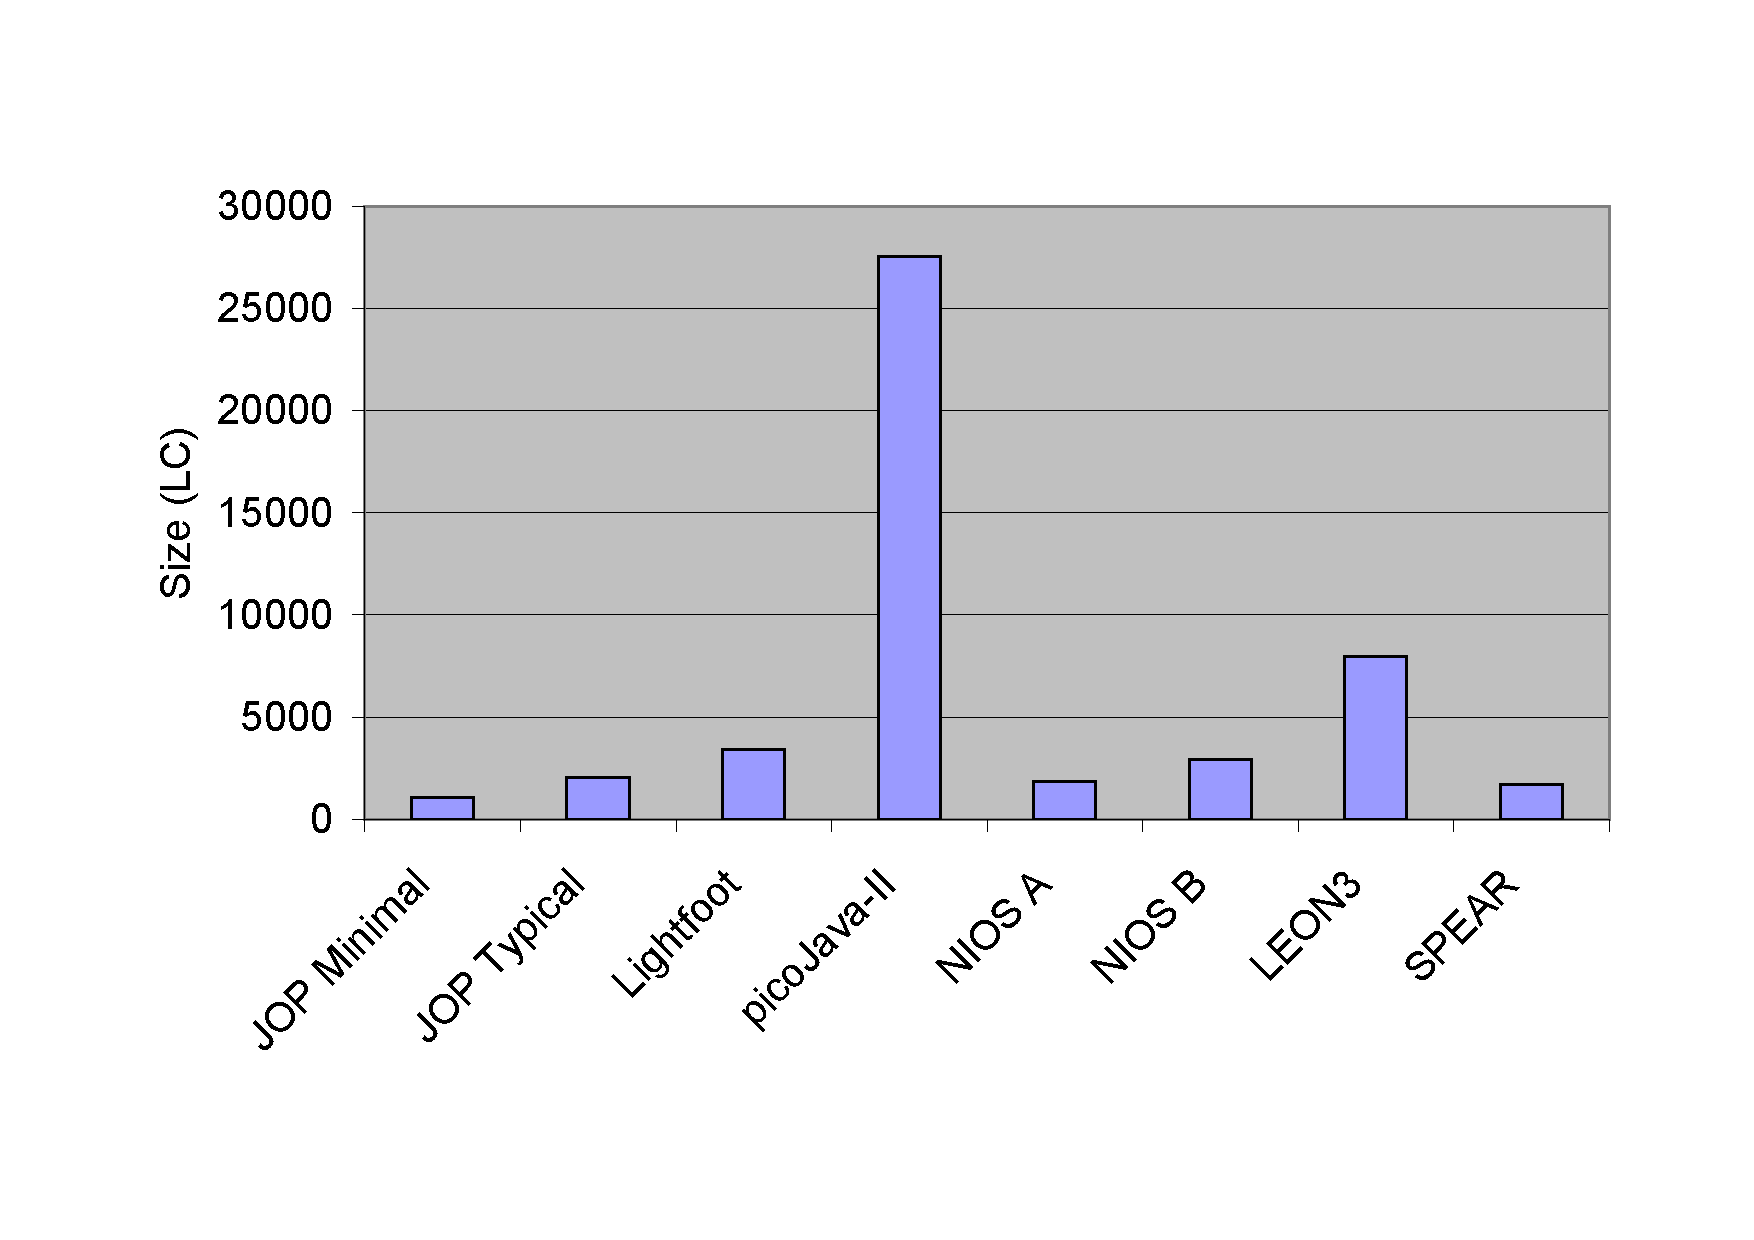
\includegraphics[width=\excelwidth]{results/size}
    \caption{Size in logic cells (LC) of different soft-core
    processors}
    \label{fig:size}
\end{figure}

One major design objective in the development of JOP was to create a
small system that can be implemented in a low-cost FPGA.
Figure~\ref{fig:size} and \tablename~\ref{tab_results_compare} show
the resource usage for different configurations of JOP and different
soft-core processors implemented in an Altera EP1C6 FPGA
\cite{AltCyc}. Estimating equivalent gate counts for designs in an
FPGA is problematic. It is therefore better to compare the two basic
structures, Logic Cells (LC) and embedded memory blocks. The maximum
frequency for all soft-core processors is in the same technology or
normalized (SPEAR) to the technology.

All configurations of JOP contain the on-chip microcode memory, the
1~KB stack cache, a 1~KB method cache, a memory interface to a
32-bit static RAM, and an 8-bit FLASH interface for the Java program
and the FPGA configuration data. The minimum configuration
implements multiplication and the shift operations in microcode. In
the typical configuration, these operations are implemented as a
sequential Booth multiplier and a single-cycle barrel shifter. The
typical configuration also contains some useful I/O devices such as
an UART and a timer with interrupt logic for multi-threading. The
typical configuration of JOP consumes about 30\% of the LCs in a
Cyclone EP1C6, thus leaving enough resources free for
application-specific logic.

As a reference, NIOS \cite{NIOS}, Altera's popular RISC soft-core, is
also included in \tablename~\ref{tab_results_compare}. NIOS has a
16-bit instruction set, a 5-stage pipeline and can be configured with
a 16 or 32-bit datapath. Version A is the minimum configuration of
NIOS. Version B adds an external memory interface, multiplication
support, and a timer. Version A is comparable with the minimal
configuration of JOP, and Version B with its typical configuration.

LEON3 \cite{LEON}, the open-source implementation of the SPARC V8
architecture, has been ported to the exact same hardware that was
used for the JOP numbers. LEON3 is representative for a RISC
processor that is used in embedded real-time systems (e.g., by ESA
for space missions).

\begin{table}
    \centering
    \begin{tabular}{lD{.}{.}{1}D{.}{.}{1.2}D{.}{.}{1}}
        \toprule
        Processor & Resources & \multicolumn{1}{c}{Memory} & \multicolumn{1}{c}{fmax} \\
                  &  (LC)    &  \multicolumn{1}{c}{(KB)} &  \multicolumn{1}{c}{(MHz)} \\
        \midrule

        JOP Minimal & 1077 & 3.25 & 98 \\
        JOP Typical & 2049 & 3.25 & 100 \\
        Lightfoot\footnotemark \cite{Lightfoot} & 3400 & 4 & 40 \\
        picoJava-II \cite{pjfpga} & 27543 & 47.6 & 43 \\
        NIOS A \cite{NIOS} & 1828 & 6.2 & 120 \\
        NIOS B \cite{NIOS} & 2923 & 5.5 & 119 \\
        LEON3 \cite{LEON} & 7978 & 10.9 & 35 \\
        SPEAR\footnotemark \cite{Delvai:ECRTS2003} & 1700 & 8 & 80 \\
        \bottomrule
    \end{tabular}
    \caption{Size and maximum frequency of FPGA soft-core processors}
    \label{tab_results_compare}
\end{table}

\addtocounter{footnote}{-1} \footnotetext{The data for the Lightfoot
processor is taken from the data sheet \cite{Lightfoot}. The
frequency used is that in a Virtex-II device from Xilinx. JOP can be
clocked at 100~MHz in the Virtex-II device, making this comparison
valid.}

\stepcounter{footnote} \footnotetext{As SPEAR uses internal memory
blocks in asynchronous mode it is not possible to synthesize it
without modification for the Cyclone FPGA. The clock frequency of
SPEAR in an Altera Cyclone is an estimate based on following facts:
SPEAR can be clocked at 40~MHz in an APEX device and JOP can be
clocked at 50~MHz in the same device.}

SPEAR \cite{Delvai:ECRTS2003} (Scalable Processor for Embedded
Applications in Real-time Environments) is a 16-bit processor with
deterministic execution times. SPEAR contains predicated
instructions to support single-path programming
\cite{Puschner:WORDS2005}. SPEAR is included in the list as it is
also a processor designed for real-time systems.

To prove that the VHDL code for JOP is as portable as possible, JOP
was also implemented in a Xilinx Spartan-3 FPGA \cite{Spartan3}.
Only the instantiation and initialization code for the on-chip
memories is vendor-specific, whilst the rest of the VHDL code can be
shared for the different targets. JOP consumes about the same LC
count (1844~LCs) in the Spartan device, but has a slower clock
frequency (83~MHz).

From this comparison we can see that we have achieved our objective
of designing a small processor. The commercial Java processor,
Lightfoot, consumes 1.7 times the logic resources of JOP in the
typical configuration (with a lower clock frequency). A typical
32-bit RISC processor (NIOS) consumes about 1.5 times (LEON about
four times) the resources of JOP. However, the NIOS processor can be
clocked 20\% faster than JOP in the same technology. The vendor
independent and open-source RISC processor LEON can be clocked only
with 35\% of JOP's frequency. The only processor that is similar in
size is SPEAR. However, while SPEAR is a 16-bit processor, JOP
contains a 32-bit datapath.


%\begin{table}
%    \centering
%    \begin{tabular}{llrr}
%        \toprule
%        JOP & Optimization & Resource [LC] & fmax [MHz] \\
%        \midrule
%        Typical (iomin) & default & 1930 & 101 \\
%         & Reg.pack: min. Area w/Chains & 1764 & 99 \\
%         & + Synth. Area & 1746 & 98 \\
%         & Reg.pack: min. Are w/Chains + Synth speed & 1800
%        & 100 \\
%        Core (no io) & Reg.pack, Synth Area & 1452 & 98 \\
%        - mul & & 1296 & 99 \\
%        - shift & with single bit sar & 1077 & 98 \\
%        \midrule
%        Typical, Spartan-3 & speed & 1844 & 83 \\
%        Typical, Spartan-3 & area & 1689 & 74 \\
%        \bottomrule
%    \end{tabular}
%    \caption{FPGA Soft Core Processors}
%    \label{tab_results_jop_versions}
%\end{table}

%Different LC/gate values:
%    from tow-level stack: 1LC = 5.4 gates
%    from ram stack: 1LC = 5.5 gates
%    from register stack: 1LC = 5.9 gates
%    Moon: 3660LCs - 27K gates + 3KB ROM + 1KB RAM: 1LC = 7.4 gates
%    Lightfoot: 3400LCs - 25K gates: 1LC = 7.4 gates
%    picoJava: ROM/RAM - 1Bit = 1 gate
%
%    JOP: 1831 LCs, 3.25KB: 1831*6 + 26624*1.5 = 11K + 39k
%    JOP: 2050*6 + 3.5*1024*8*1.5 = 12K + 43K
%    Pentium MMX: 4.5 Mio. Transistors -> 1100K

Table~\ref{tab:results:gate:count} provides gate count estimates for
JOP, picoJava, the aJile processor, and the Intel Pentium MMX
processor that is used in the benchmarks in the next section.
Equivalent gate count for an LC\footnote{The factors are derived
from the data provided for various processors in
Chapter~\ref{chap:related} and from the resource estimates in
Section~\ref{sec:stack}.} varies between 5.5 and 7.4 -- we chose a
factor of 6 gates per LC and 1.5 gates per memory bit for the
estimated gate count for JOP in the table. JOP is listed in the
typical configuration that consumes 2050 LCs. The Pentium MMX
contains 4.5M transistors \cite{pentium:mmx} that are equivalent to
1125K gates.

\begin{table}
    \centering
    \begin{tabular}{lrrr}
        \toprule
        Processor & \multicolumn{1}{c}{Core} & \multicolumn{1}{c}{Memory} & \multicolumn{1}{c}{Sum.} \\
        & \multicolumn{1}{c}{[gate]} & \multicolumn{1}{c}{[gate]} & \multicolumn{1}{c}{[gate]}\\
        \midrule
        JOP & 12K & 43K & 55K\\
        picoJava & 128K & 314K & 442K\\
        aJile & 25K & 912K & 937K\\
        Pentium MMX & & & 1125K\\
        \bottomrule
    \end{tabular}
    \caption{Gate count estimates for various processors}
    \label{tab:results:gate:count}
\end{table}

We can see from the table that the on-chip memory dominates the
overall gate count of JOP, and to an even greater extent, of the
aJile processor. The aJile processor is roughly the same size as the
Pentium MMX, and both are about 20 times larger than JOP.


\section{Performance}
\label{sec:performance}

In this section, we will evaluate the performance of JOP in relation
to other Java systems. Although JOP is intended as a processor with
a low WCET for all operations, its general performance is still
important. In the first section, we will evaluate JOP's average
performance.

%In the section that follows it, the implementation of the simple
%real-time profile, as described in Section~\ref{sec:rtprof}, on JOP
%is compared to the RI of the RTSJ on top of Linux.

The comparison of the implementation of the simple real-time profile,
as described in Section~\ref{sec:rtprof}, on JOP with the RI of the
RTSJ on top of Linux can be found in \cite{jop:rtjava}.

\subsection{General Performance}

Running benchmarks is problematic, both generally and especially in
the case of embedded systems. The best benchmark would be the
application that is intended to run on the system being tested. To
get comparable results, SPEC provides benchmarks for various systems.
However, the one for Java, the SPECjvm98 \cite{SPECJvm98}, needs more
functionality than what is usually available in a CLDC compliant
device (e.g., a filesystem and \code{java.net}). Some benchmarks from
the SPECjvm98 suites also need several megabaytes of heap.

Due to the absence of a \emph{standard} Java benchmark for embedded
systems, a small benchmark suite that should run on even the
smallest device is provided here. It contains several
micro-benchmarks for evaluating the number of clock cycles for
single bytecodes or short sequences of bytecodes, and two
application benchmarks.

To provide a realistic workload for embedded systems, a real-time
application was adapted to create the first application benchmark
(Kfl). The application is taken from one of the nodes of a
distributed motor control system \cite{jop:wises03} (the first
industrial application of JOP). The application is written as a
cyclic executive. A simulation of both the environment (sensors and
actors) and the communication system (commands from the master
station) forms part of the benchmark, so as to simulate the
real-world workload. The second application benchmark is an
adaptation of a tiny TCP/IP stack for embedded Java. This benchmark
contains two UDP server/clients, exchanging messages via a loopback
device. The Kfl benchmark consists of 511 methods and 14~KB code,
the UDP/IP benchmark of 508 methods and 13~KB code (including the
supporting library).

As we will see, there is a great variation in processing power
across different embedded systems. To cater for this variation, all
benchmarks are `self adjusting'. Each benchmark consists of an
aspect that is benchmarked in a loop and an `overhead' loop that
contains any overheads from the benchmark that should be subtracted
from the result (this feature is designed for the micro-benchmarks).
The loop count adapts itself until the benchmark runs for more than
a second. The number of iterations per second is then calculated,
which means that higher values indicate better performance.

%Teilweise Wiederholung

All the benchmarks measure how often a function is executed per
second. In the Kfl benchmark, this function contains the main loop of
the application that is executed in a periodic cycle in the original
application. In the benchmark, the wait for the next period is
omitted, so that the time measured solely represents execution time.
The UDP benchmark contains the generation of a request, transmitting
it through the UDP/IP stack, generating the answer and transmitting
it back as a benchmark function. The iteration count is the number of
received answers per second.

The accuracy of the measurement depends on the resolution of the
system time. For the measurements under Linux, the system time has a
resolution of 10ms, resulting in an inaccuracy of 1\%. The accuracy
of the system time on leJOS, TINI and the aJile is not known, but is
considered to be in the same range. For JOP, a $\mu$s counter is
used for time measurement.


The following list gives a brief description of the Java systems
that were benchmarked:

\begin{description}
    \item[JOP]
is implemented in a Cyclone FPGA \cite{AltCyc}, running at 100~MHz.
The main memory is a 32-bit SRAM (15ns) with an access time of 2
clock cycles. The benchmarked configuration of JOP contains a 4~KB
method cache organized in 16 blocks.

    \item[leJOS] As an example for a low-end embedded device, we
        use the RCX robot controller from the LEGO MindStorms
        series. It contains a 16-bit Hitachi H8300
        microcontroller \cite{hitachi:h8}, running at 16~MHz.
        leJOS \cite{lejos} is a tiny interpreting JVM for the
        RCX.

    \item[KVM] is a port of Sun's KVM, is part of the Connected
        Limited Device Configuration (CLDC) \cite{J2ME}, to
        Altera's NIOS II processor on MicroC Linux. NIOS is
        implemented on a Cyclone FPGA and clocked at 50~MHz.
        Besides the different clock frequency, this is a good
        comparison of an interpreting JVM running in the same
        FPGA as JOP.

    \item[TINI]
is an enhanced 8051 clone running a software JVM. The results were
taken from a custom board with a 20~MHz crystal, and the chip's PLL
is set to a factor of 2.

    \item[Cjip]
The measured system \cite{SNAP} is a replacement of the TINI board
and contains a Cjip \cite{Cjip} clocked with 80~MHz and 8~MB DRAM.

    \item[Komodo]
Komodo \cite{komodo2003} is a Java processor as a basis for research
on real-time scheduling on a multithreaded microcontroller (see
Section~\ref{subsec:related:komodo}). The benchmark results were
obtained by Matthias Pfeffer \cite{Pfeffer} on a cycle-accurate
simulation of Komodo. The values are obtained without garbage
collection. According to Pfeffer, Komodo can be clocked with 33MHz
in a Xlinix XCV800.

    \item[aJile] aJile's JEMCore is a direct-execution Java
        processor that is available in two different versions:
        the \textbf{aJ80} and the \textbf{aJ100} \cite{aJile}.
        The aJ100 provides a generic 8-bit, 16-bit, or 32-bit
        external bus interface, while the aJ80 only provides an
        8-bit interface.


    \item[EJC]
The Embedded Java Controller (EJC) platform \cite{EJC} is a typical
example of a JIT system on a RISC processor. The system is based on
a 32-bit ARM720T processor running at 74~MHz. It contains up to
64~MB SDRAM and up to 16~MB of NOR flash.

    \item[gcj]
is the GNU compiler for Java. This configuration represents the
batch compiler solution, running on a 266~MHz Pentium MMX under
Linux.

    \item[MB]
is the realization of Java on a RISC processor for an FPGA (Xilinx
MicroBlaze \cite{microblaze}). Java is compiled to C with a Java
compiler for real-time systems \cite{Java2C} and the C program is
compiled with the standard GNU toolchain.

\end{description}

It would be interesting to include the other soft-core Java
processors (Moon, Lightfoot, and FemtoJava) in this comparison.
However, it was not possible to obtain the benchmark data. The
company that produced Moon seems to have disappeared and FemtoJava
could not run all benchmarks.


\begin{figure}
    \centering
    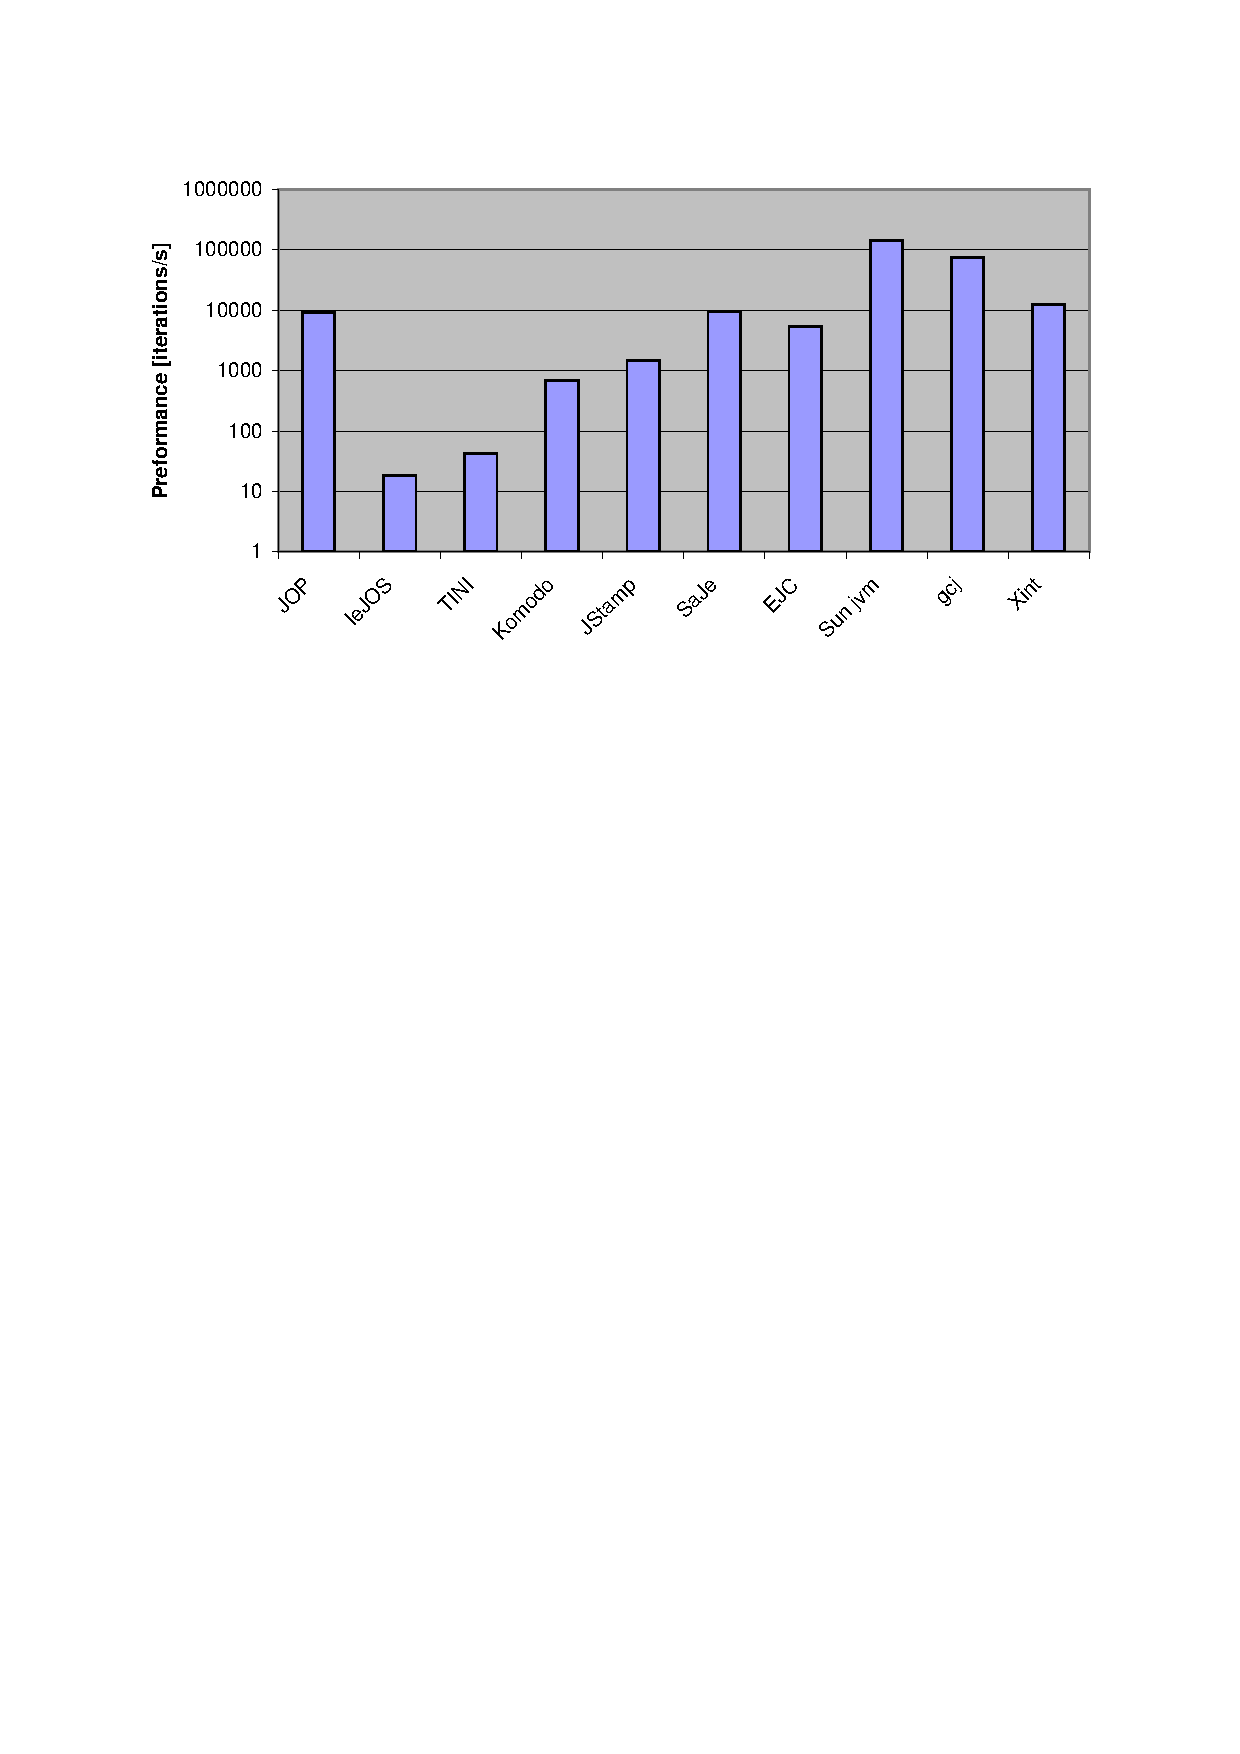
\includegraphics[width=\excelwidth]{results/results_app_bench}
    \\
    \vspace{0.5cm}
    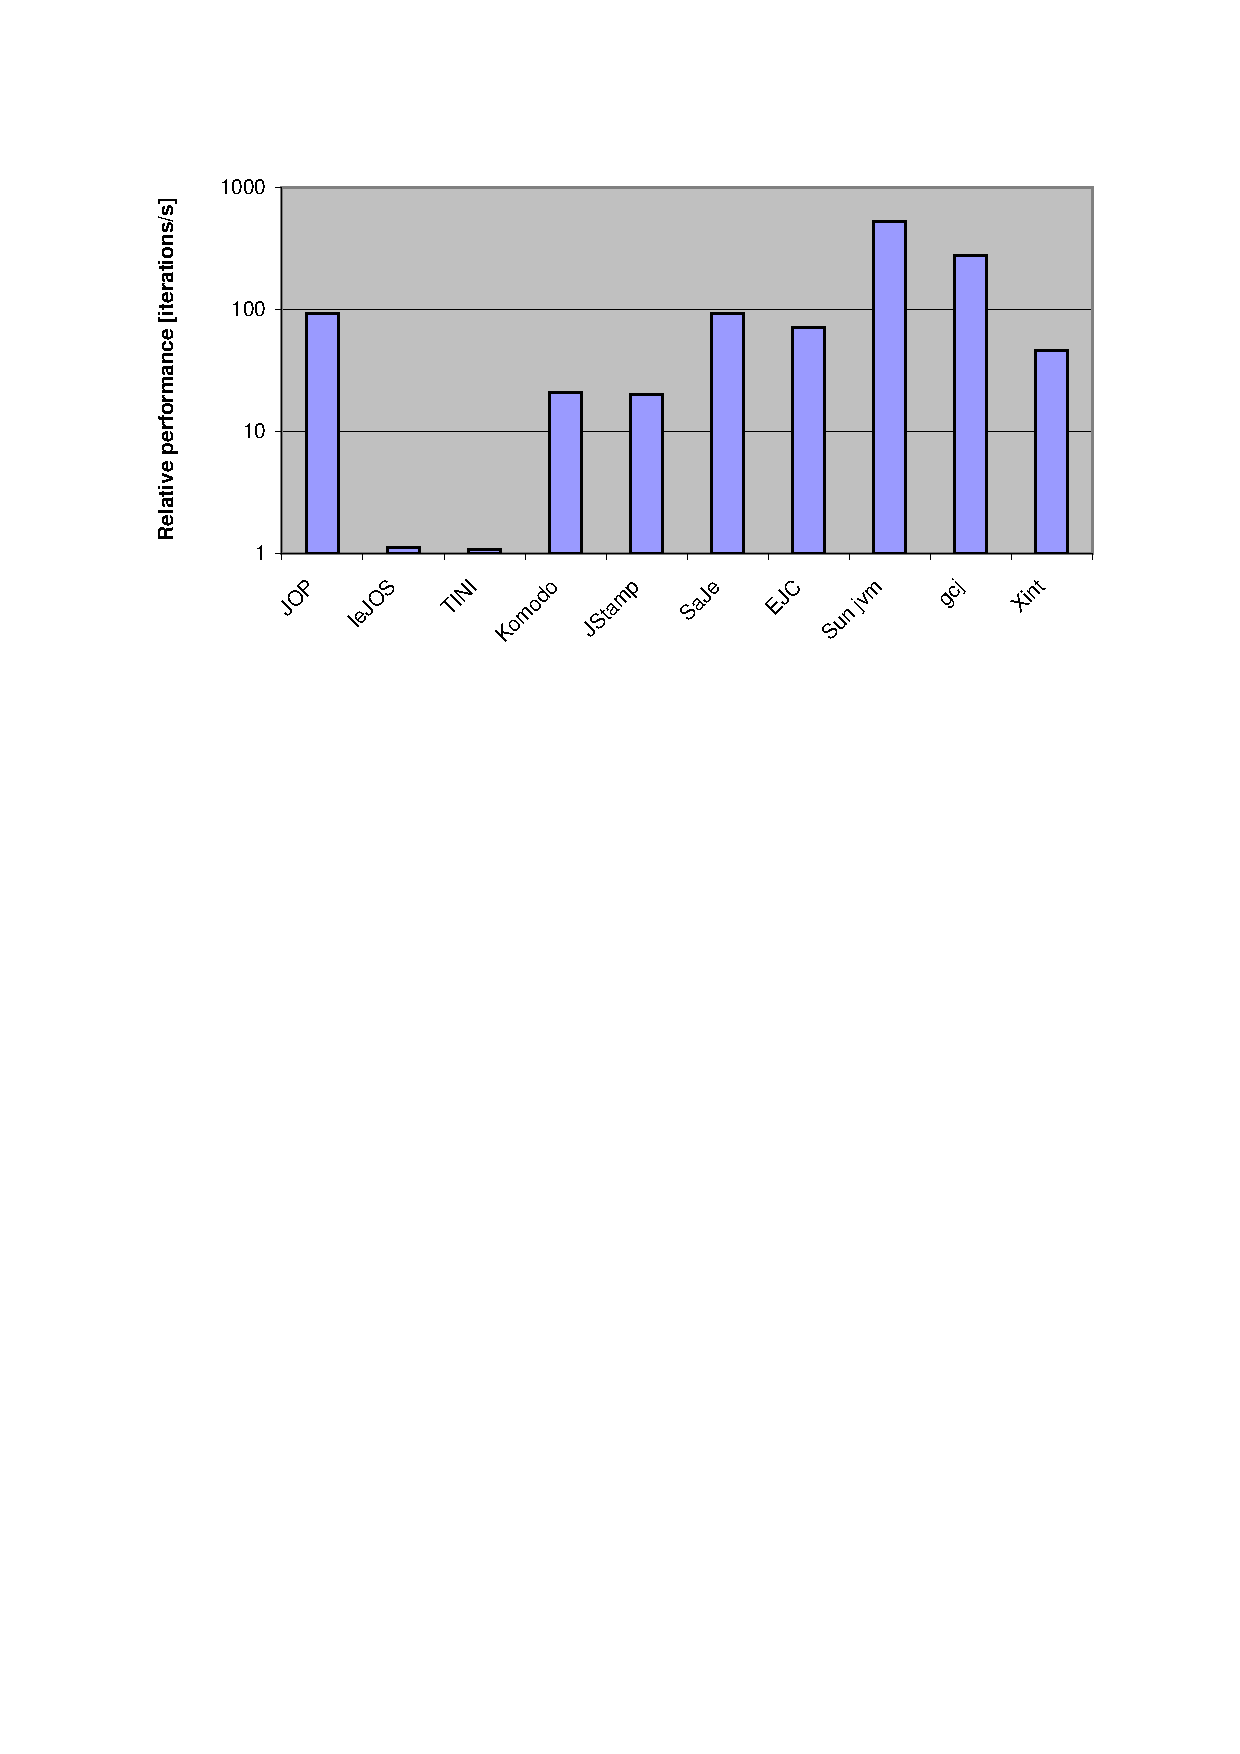
\includegraphics[width=\excelwidth]{results/results_app_bench_scaled}
    \caption{Performance comparison of different Java systems with
    application benchmarks. The diagrams show the geometric mean
    of the two benchmarks in iterations per second -- a higher
    value means higher performance. The top diagram shows
    absolute performance, while the bottom diagram shows the result
    scaled to 1~MHz clock frequency.
    }
    \label{fig:results:app:bench}
\end{figure}


In Figure~\ref{fig:results:app:bench}, the geometric mean of the two
application benchmarks is shown. The unit used for the result is
iterations per second. Note that the vertical axis is logarithmic,
in order to obtain useful figures to show the great variation in
performance. The top diagram shows absolute performance, while the
bottom diagram shows the same results scaled to a 1~MHz clock
frequency. The results of the application benchmarks and the
geometric mean are shown in \tablename~\ref{tab:results:bench:app}.


It should be noted that scaling to a single clock frequency could
prove problematic. The relation between processor clock frequency
and memory access time cannot always be maintained. To give an
example, if we were to increase the results of the 100~MHz JOP to
1~GHz, this would also involve reducing the memory access time from
15~ns to 1.5~ns. Processors with 1~GHz clock frequency are already
available, but the fastest asynchronous SRAM to date has an access
time of 10~ns.

%To compare the performance relatively to the size of the different
%systems, Figure~\ref{fig:results:app:bench:double:scaled} shows the
%performance of JOP, the aJ100 and the gcj PC versions relative to
%the gate count (from Table~\ref{tab:results:gate:count}) and clock
%frequency. Relative to size and clock frequency, JOP outperforms the
%aJile processor by a factor of 20 and even the gcj-compiler on the
%Pentium MMX by a factor of 8.





\begin{table}
    \centering
    \begin{tabular*}{\columnwidth}{@{\extracolsep{\fill}}lD{.}{.}{2}rrD{.}{.}{2}D{.}{.}{2}}
%    \begin{tabular}{lrrrrrr}
        \toprule

 & \multicolumn{1}{c}{Frequency} & \multicolumn{1}{c}{Kfl} & \multicolumn{1}{c}{UDP/IP}
    & \multicolumn{1}{c}{Geom. Mean} & \multicolumn{1}{c}{Scaled}\\
 &  \multicolumn{1}{c}{(MHz)} &  \multicolumn{4}{c}{(Iterations/s)}\\
        \midrule
JOP & 100 & 17111 & 6781 & 10772 & 108\\
leJOS & 16 & 25 & 13 & 18 & 1.1\\
TINI & 40 & 64 & 29 & 43 & 1.1\\
KVM & 50 & 36 & 16 & 24 & 0.5\\
Cjip & 80 & 176 & 91 & 127 & 1.6\\
Komodo & 33 & 924 & 520 & 693 & 21\\
aJ80 & 74 & 2221 & 1004 & 1493 & 20\\
aJ100 & 103 & 14148 & 6415 & 9527 & 92\\
EJC & 74 & 9893 & 2822 & 5284 & 71\\
%Sun jvm & 266 & 212,952 & 91,851 & 139,857 & 526\\
gcj & 266 & 139884 & 38460 & 73348 & 276\\
%Xint & 266 & 17,310 & 8,747 & 12,305 & 46\\
MB & 100 & 3792 &  &  & \\
% MB 8KB/8KB & 100 & 25,090 &  &  & \\
        \bottomrule

    \end{tabular*}
    \caption{Application benchmarks on different Java systems.
    The table shows the benchmark results in
    iterations per second -- a higher
    value means higher performance.
    }
    \label{tab:results:bench:app}
\end{table}

% not
%\begin{figure}
%    \centering
%    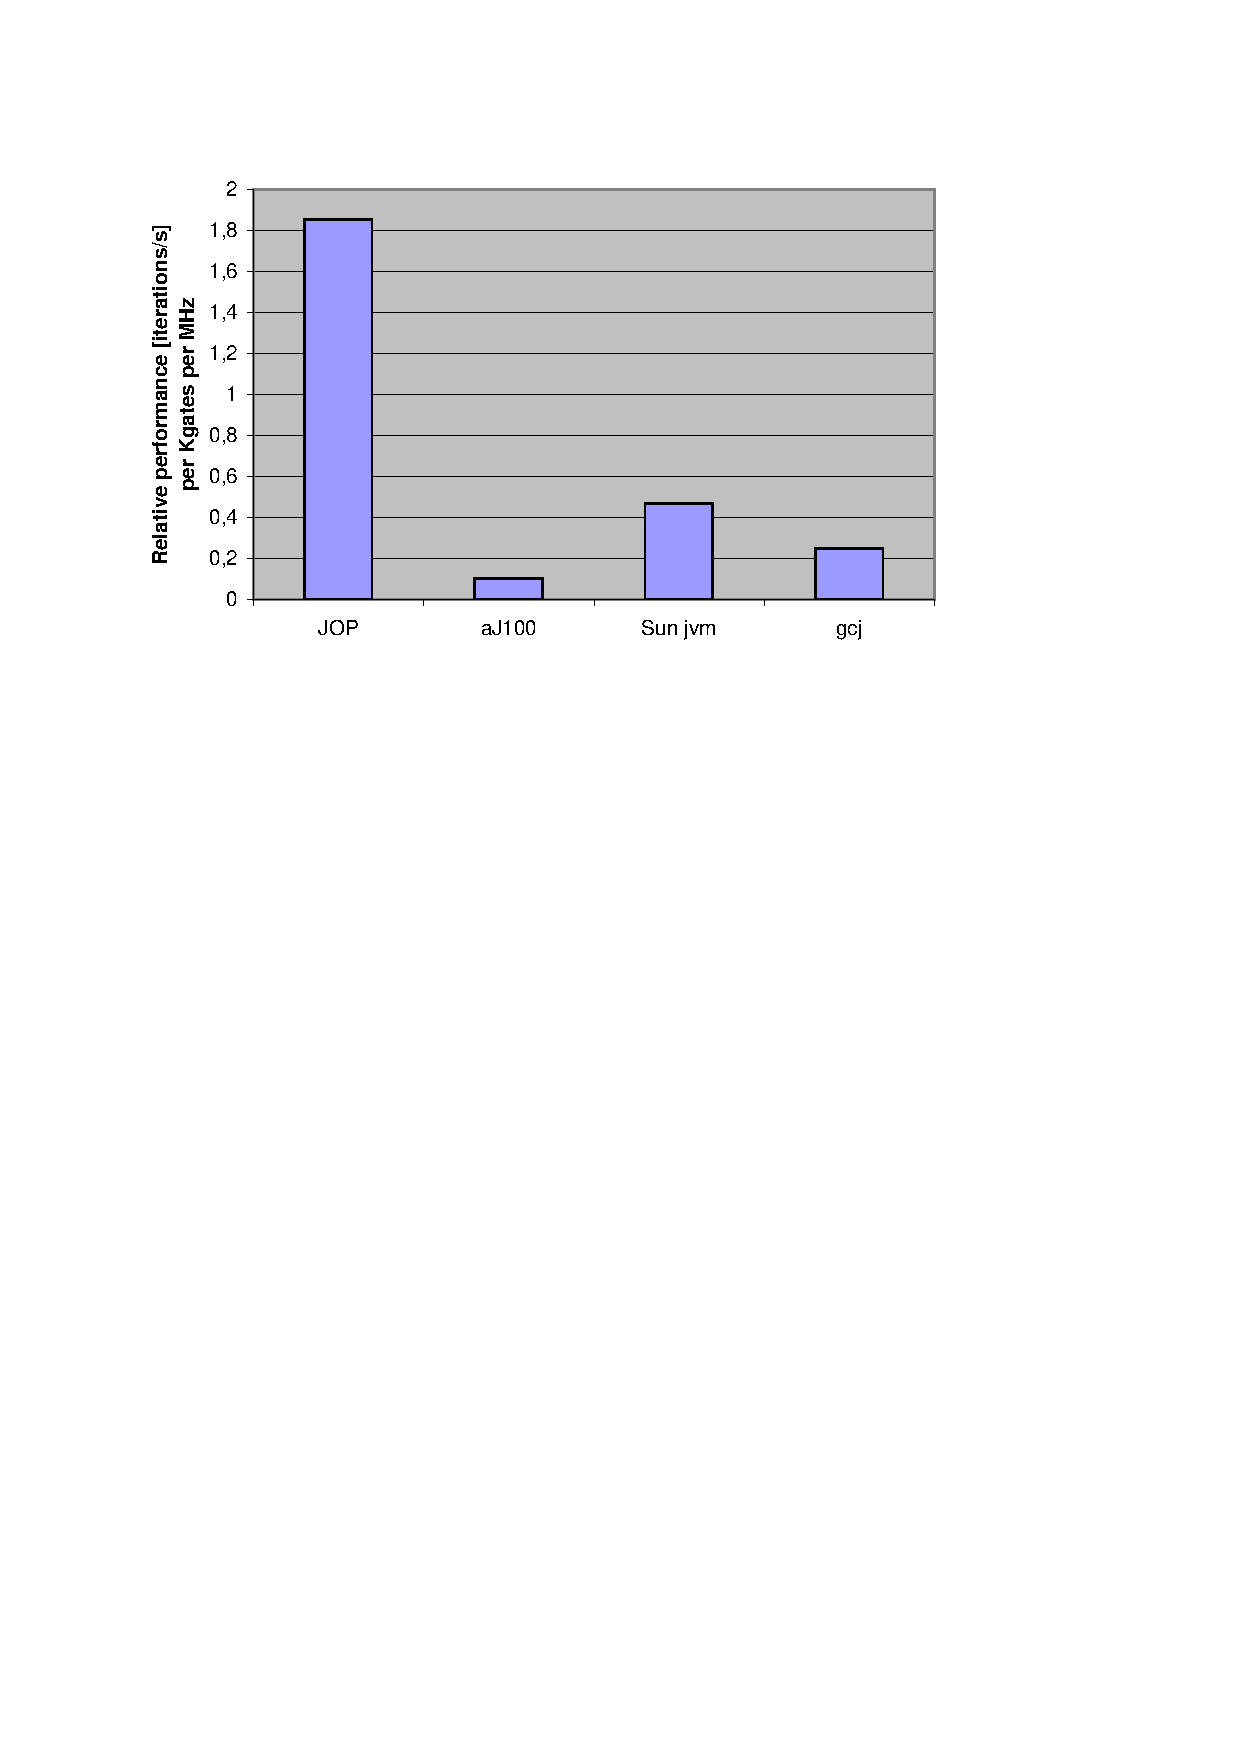
\includegraphics[width=\excelwidth]{results_app_bench_double_scaled}
%    \caption{Performance comparison of different Java systems with
%    application benchmarks. The diagram shows the result scaled to
%    the chip size (Kgates) and clock frequency (MHz).
%    }
%    \label{fig:results:app:bench:double:scaled}
%\end{figure}


\subsection{Discussion}
\label{sec:perf:disc}

When comparing JOP and the aJile processor against leJOS, KVM, and
TINI, we can see that a Java processor is up to 500 times faster
than an interpreting JVM on a standard processor for an embedded
system. The average performance of JOP is even better than a
JIT-compiler solution on an embedded system, as represented by the
EJC system.

Even when scaled to the same clock frequency, the compiling JVM on a
PC (gcj) is much faster than either embedded solution. However, the
kernel of the application is smaller than 4~KB
\cite{jop:jtres_cache}. It therefore fits in the level one cache of
the Pentium MMX. For a comparison with a Pentium class processor we
would need a larger application.

JOP is about 7 times faster than the aJ80 Java processor on the
popular JStamp board. However, the aJ80 processor only contains an
8-bit memory interface, and suffers from this bottleneck. The SaJe
system contains the aJ100 with 32-bit, 10~ns SRAMs. JOP with its
15~ns SRAMs is about 12\% faster than the aJ100 processor.

The MicroBlaze system is a representation of a Java batch-compilation
system for a RISC processor. MicroBlaze is configured with the same
cache\footnote{The MicroBlaze with an 8~KB data and 8~KB instruction
cache is about 1.5 times faster than JOP. However, a 16~KB memory is
not available in low-cost FPGAs and is an unbalanced system with
respect to the LC/memory relation.} as JOP and clocked at the same
frequency. JOP is about four times faster than this solution, thus
showing that native execution of Java bytecodes is faster than
batch-compiled Java on a similar system. However, the results of the
MicroBlaze solution are at a preliminary stage\footnote{As not all
language constructs can be compiled, only the Kfl benchmark was
measured. Therefore, the bars for MicroBlaze are missing in
\figurename~\ref{fig:results:app:bench}.}, as the Java2C compiler
\cite{Java2C} is still under development.

The micro-benchmarks are intended to give insight into the
implementation of the JVM. In Table~\ref{tab:results:bench:clock},
we can see the execution time in clock cycles of various bytecodes.
As almost all bytecodes manipulate the stack, it is not possible to
measure the execution time for a single bytecode in the benchmark
loop. The single bytecode would trash the stack. As a minimum
requirement, a second instruction is necessary in the loop to
reverse the stack operation.

\begin{table}
    \centering
    \begin{tabular*}{\columnwidth}{@{\extracolsep{\fill}}lrrrrrrrr}
        \toprule

                      & JOP & leJOS & TINI  & Cjip & Komodo & aJ80 & aJ100 \\
        \midrule
    iload iadd         & 2 & 836 & 789      & 55 & 8 & 38 & 8 \\
    iinc               & 8 & 422 & 388      & 46 & 4 & 41 & 11 \\
    ldc                & 9 & 1340 & 1128  & 670 & 40 & 67 & 9 \\
    if\_icmplt taken   & 6 & 1609 & 1265  & 157 & 24 & 42 & 18 \\
    if\_icmplt n/taken & 6 & 1520 & 1211  & 132 & 24 & 40 & 14 \\
    getfield           & 22 & 1879 & 2398 & 320 & 48 & 142 & 23 \\
    getstatic          & 15 & 1676 & 4463 & 3911 & 80 & 102 & 15 \\
    iaload             & 36 & 1082 & 1543 & 139 & 28 & 74 & 13 \\
    invoke             & 128 & 4759 & 6495& 5772 & 384 & 349 & 112 \\
    invoke static      & 100 & 3875 & 5869& 5479 & 680 & 271 & 92 \\
    invoke interface   & 144 & 5094 & 6797& 5908 & 1617 & 531 & 148 \\

        \bottomrule
    \end{tabular*}
    \caption{Execution time in clock cycles for various JVM bytecodes}
    \label{tab:results:bench:clock}
\end{table}

For JOP we can deduce that the WCET for simple bytecodes  is also the
average execution time. We can see that the combination of
\code{iload} and \code{iadd} executes in two cycles, which means that
each of these two operations is executed in a single cycle. The
\code{iinc} bytecode is one of the few instructions that does not
manipulate the stack and can be measured alone. As \code{iinc} is not
implemented in hardware, we have a total of 8 cycles that are
executed in microcode. It is fair to assume that this comprises too
great an overhead for an instruction that is found in every iterative
loop with an integer index. However, the decision to implement this
instruction in microcode was derived from the observation that the
dynamic instruction count for \code{iinc} is only 2\% (see
Section~\ref{sec:bench:jvm}).

The sequence for the branch benchmark (\code{if\_icmplt}) contains
the two load instructions that push the arguments onto the stack.
The arguments are then consumed by the branch instruction. This
benchmark verifies that a branch requires a constant four cycles on
JOP, whether it is taken or not.

The Cjip implements the JVM with a stack oriented instruction set. It
is the only example (except JOP) where the instruction set is
documented \emph{including} the execution time \cite{CjipRef}. We
will therefore check some of the results with the numbers provided in
the documentation. The execution time is given in nanoseconds,
assuming a 66~MHz clock. The execution time for the basic integer add
operation is given as 180~ns resulting in 12 cycles. The load of a
local variable (when it is one of the first four) takes 35 cycles. In
the micro-benchmark we measure 55 cycles instead of the theoretical
47 (\code{iadd} + \code{iload\_n}). We assume that we have to add
some cycles for the fetch of the bytecodes from memory.

For compiling versions of the JVM, these micro-benchmarks do not
produce useful results. The compiler performs optimizations that
make it impossible to measure execution times at this fine a
granularity.

During the evaluation of the aJile system, unexpected behavior was
observed. The aJ80 on the JStamp board is clocked at 7.3728~MHz, and
the internal frequency can be set with a PLL. The aJ80 is rated for
80MHz and the maximum PLL factor that can be used is therefore ten.
Running the benchmarks with different PLL settings gave some strange
results. For example, with a PLL multiplier setting of ten, the aJ80
was about 12.8 times faster! Other PLL factors also resulted in a
greater than linear speedup. The only explanation we could find was
that the internal time, \code{System.currentTimeMillis()}, used for
the benchmarks depends on the PLL setting. A comparison with the wall
clock time showed that the internal time of the aJ80 is 23\% faster
with a PLL factor of 1 and 2.4\% faster with a factor of ten -- a
property we would not expect on a processor that is marketed for
real-time systems.

The SaJe board is also clocked with 7.3728~MHz and the PLL factor is
set to 14. This gives a 103.2192~MHz internal clock frequency.
However, it is not known how accurate the internal time is in this
setting. The results for the SaJe board can also suffer from the
problem described above.

% aJ80 at 7.3728MHz: internal 11' are external 8'57'' ... 1.23 times too fast
% aJ80 at 73.728MHz: internal 21' are external 20'30'' ... 1.024 times too fast




\subsection{Execution Time Jitter}

For real-time systems, the worst-case of the execution time is of
primary importance. We have measured the execution times of several
iterations of the main function from the Kfl benchmark.
\figurename~\ref{fig:results:kfl:exe} shows the measurements, scaled
to the minimum execution time.

\begin{figure}
    \centering
    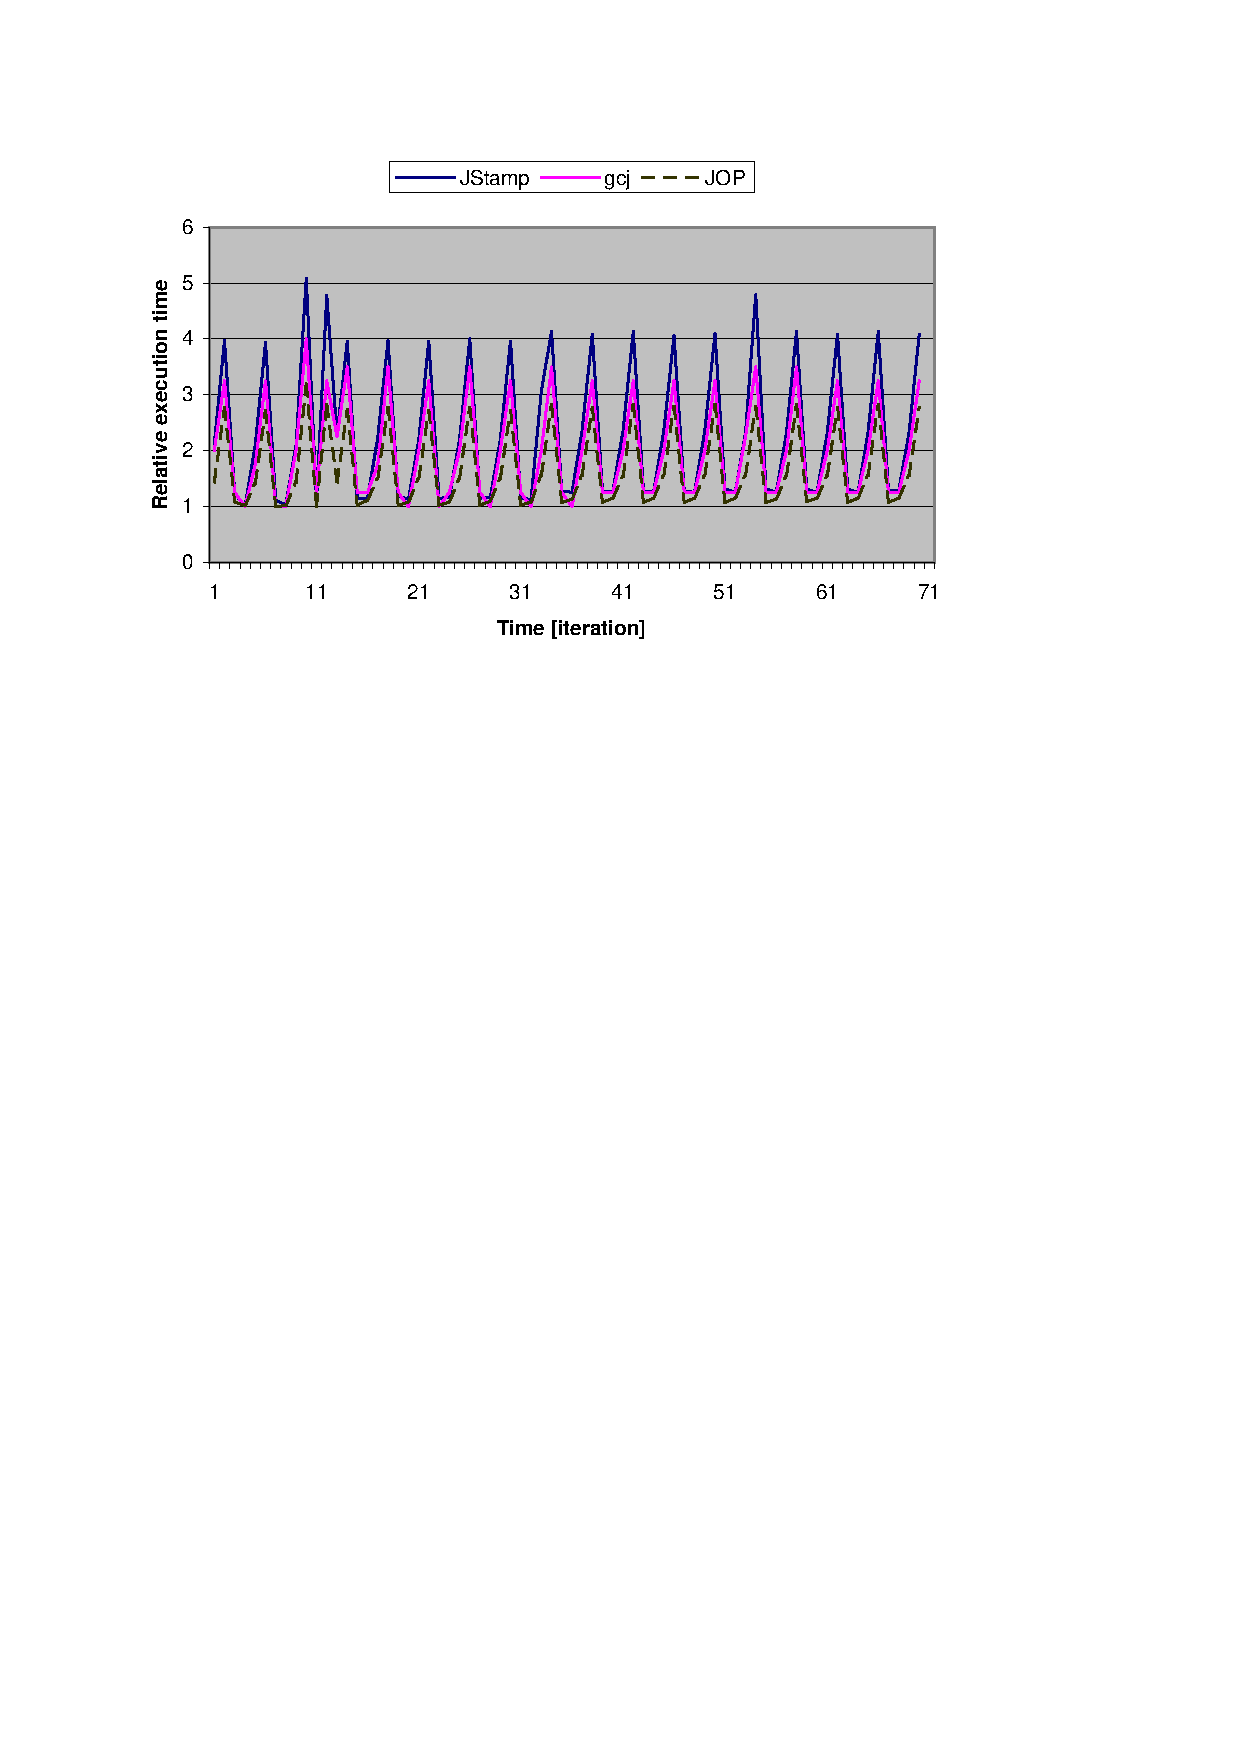
\includegraphics[width=\excelwidth]{results/results_kfl_exe}
    \\
    \vspace{0.5cm}
    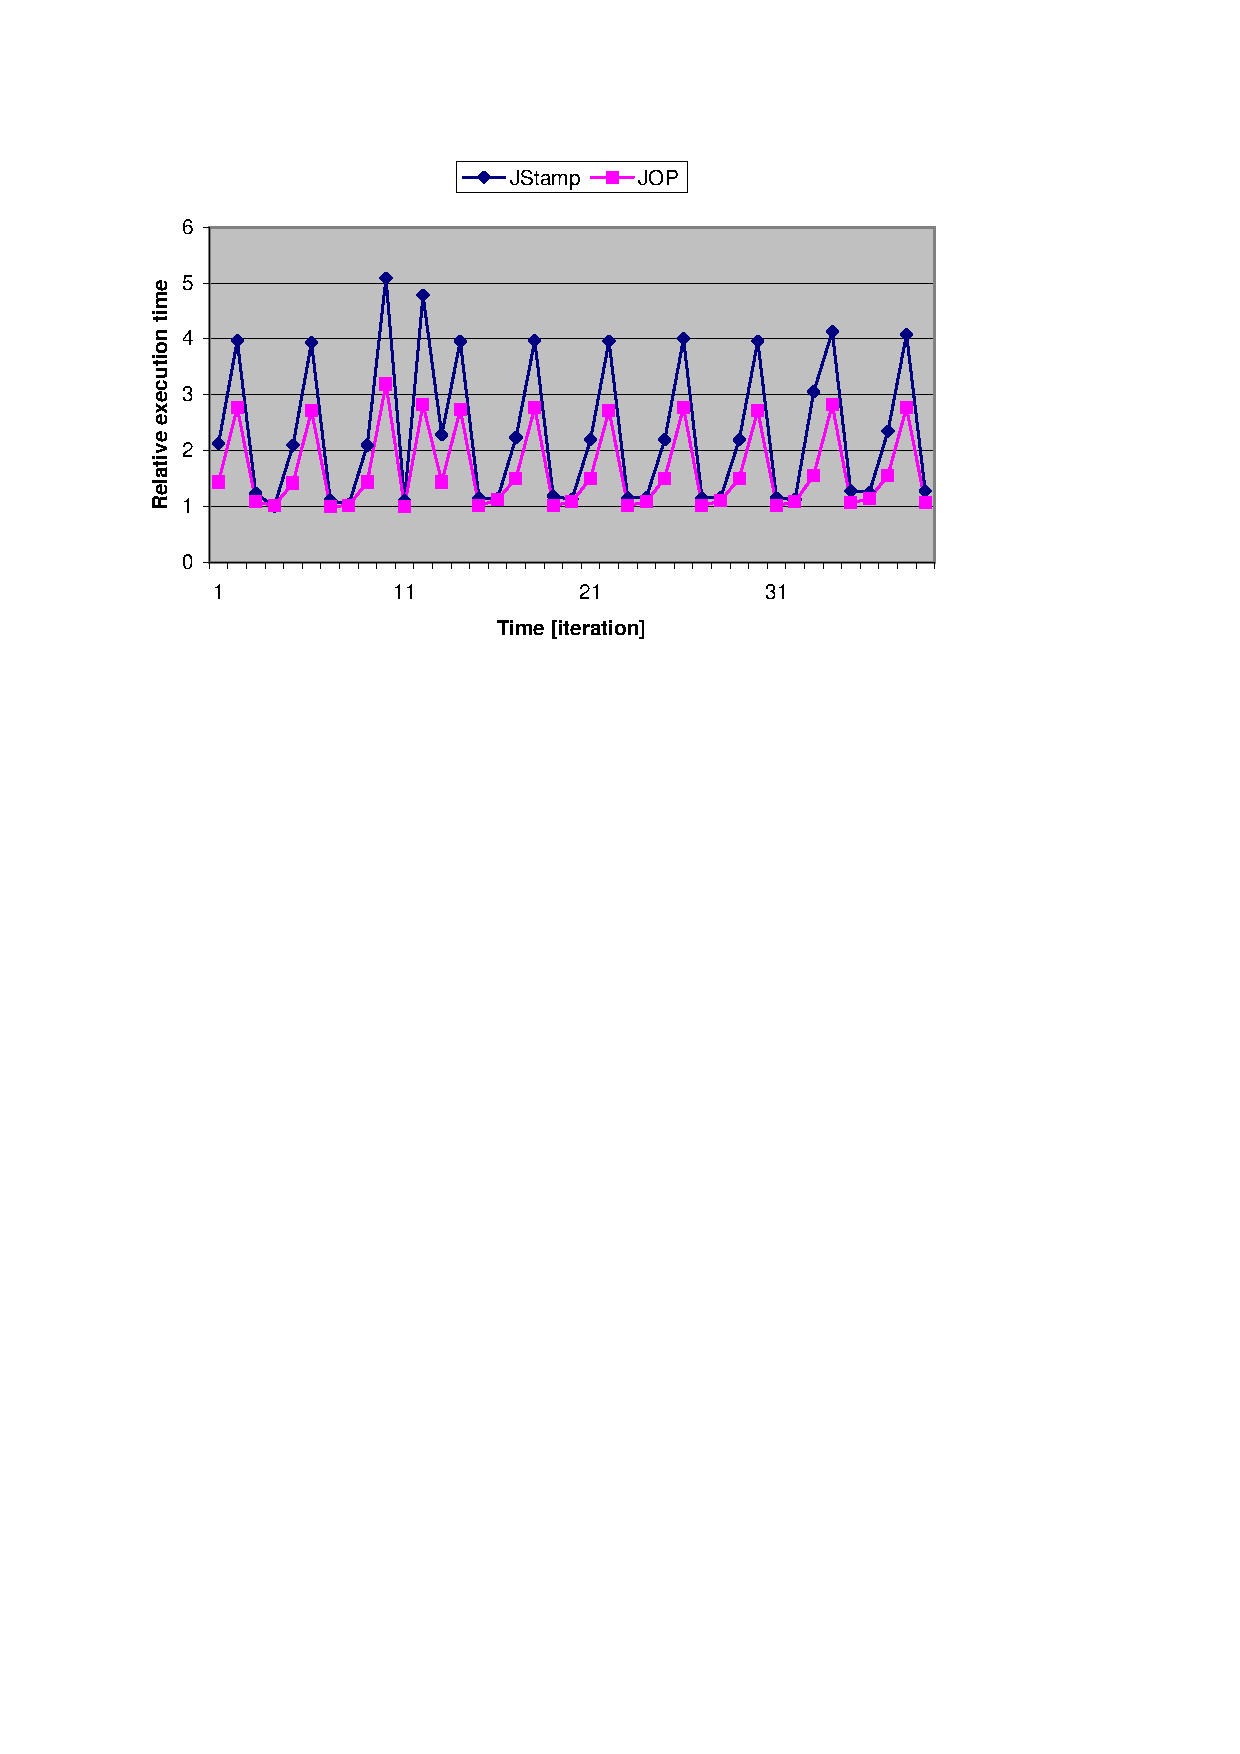
\includegraphics[width=\excelwidth]{results/results_kfl_exe_detail}
    \caption{Execution time of the main function for the Kfl benchmark.
    The values are scaled to the minimum execution time. The bottom
    figure shows a detail of the top figure.
    }
    \label{fig:results:kfl:exe}
\end{figure}

%\begin{figure}
%    \centering
%    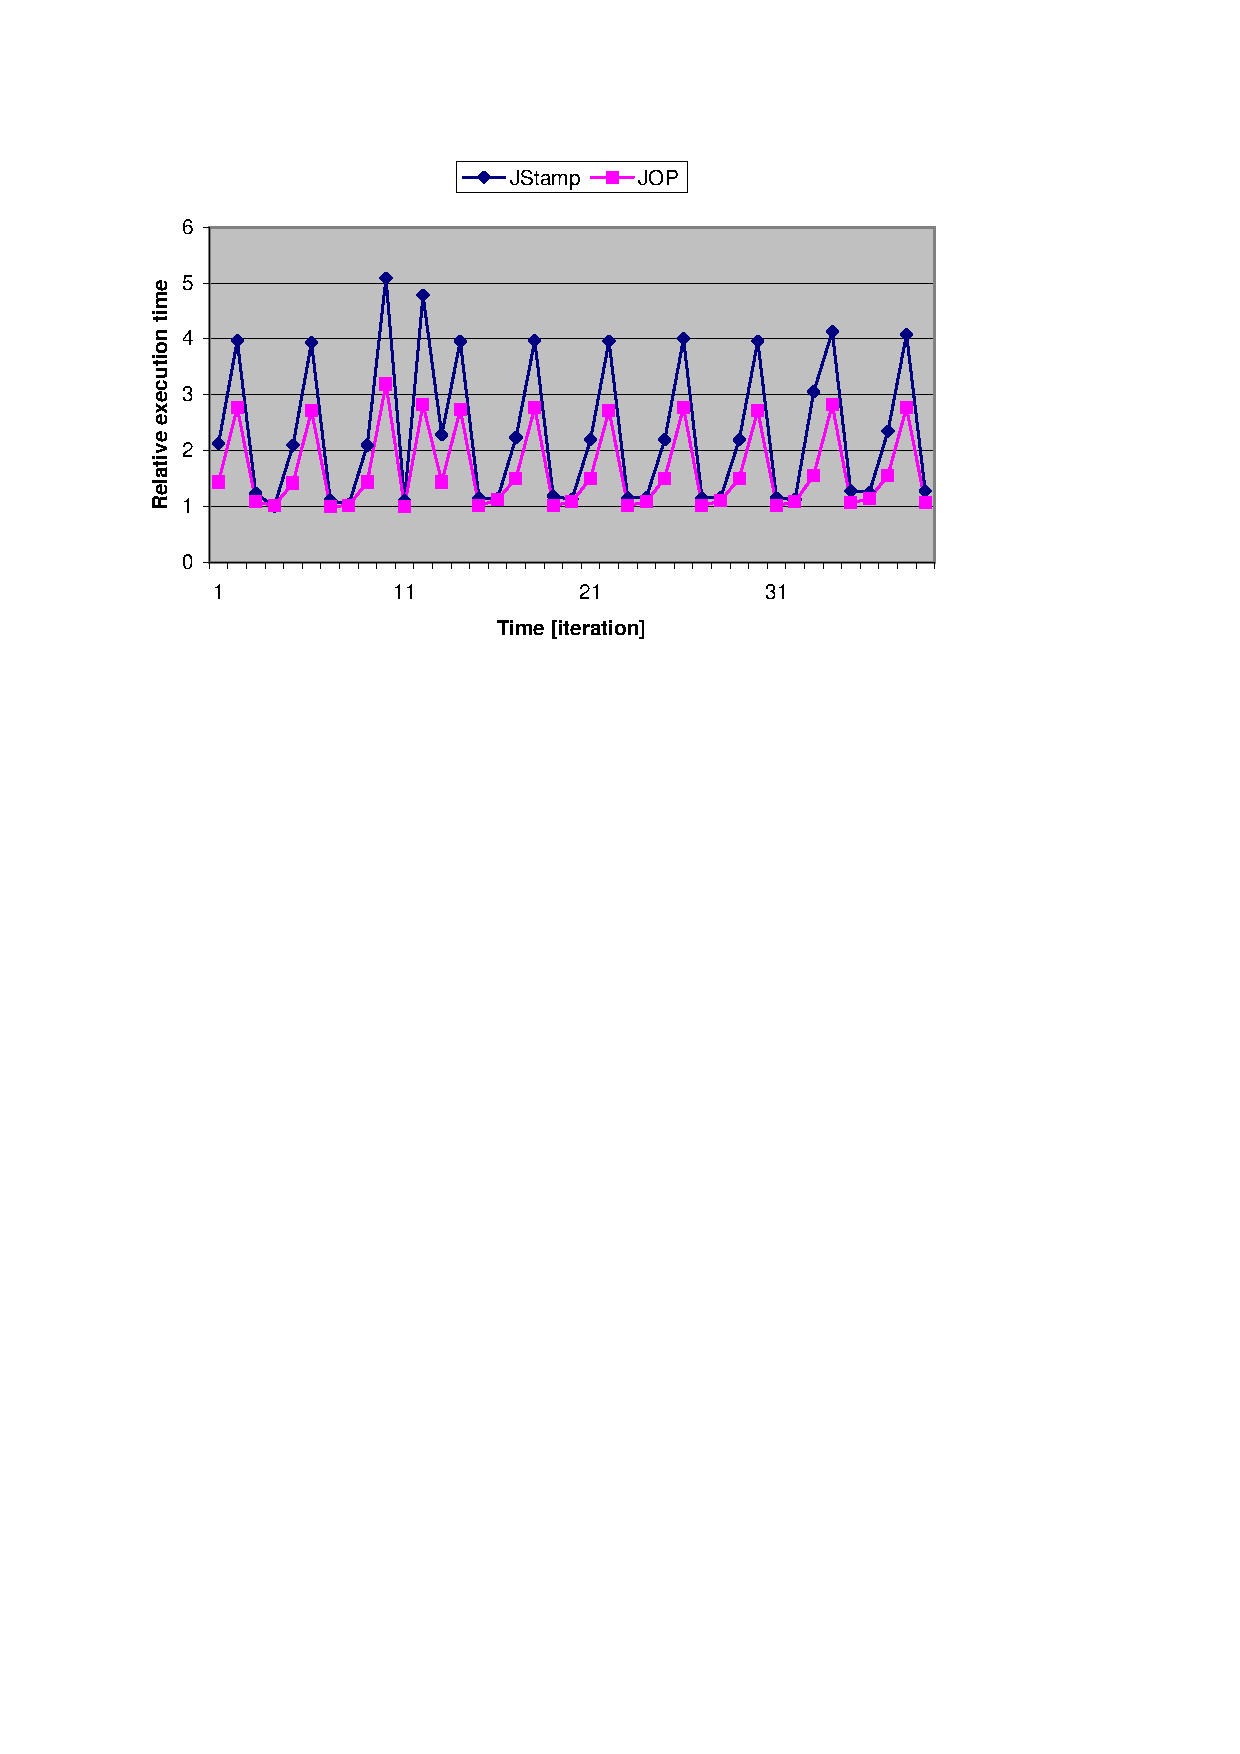
\includegraphics{results/results_kfl_exe_detail}
%    \caption{Execution time with KFL benchmark (detail).}
%    \label{fig:results:kfl:exe:detail}
%\end{figure}

A period of four iterations can be seen. This period results from
simulating the commands from the base station that are executed
every fourth iteration. At iteration 10, a command to start the
motor is issued. We see the resulting rise in execution time at
iteration 12 to process this command. At iteration 54, the
simulation triggers the end sensor and the motor is stopped.

The different execution times in the different modes of the
application are inherent in the design of the simulation. However,
the ratio between the longest and the shortest period is five for the
JStamp, four for the gcj system, and only three for JOP. Therefore, a
system with an aJile processor needs to be 1.7 times faster than JOP
in order to provide the same WCET for this measurement. At iteration
33, we can see a higher execution time for the JStamp system that is
not seen on JOP. This variation at iteration 33 is not caused by the
benchmark.

The execution time under gcj on the Linux system showed some very
high peaks (up to ten times the minimum, not shown in the figures).
This observation was to be expected, as the gcj/Linux system is not
a real-time solution. The Sun JIT-solution is omitted from the
figure. As a result of the invocation of the compiler at some point
during the simulation, the worst-case ratio between the maximum and
minimum execution time was 1313 -- showing that a JIT-compiler is
impractical for real-time applications.

It should be noted that execution time measurement is not a safe
method for obtaining WCET estimates. However, in situations where no
WCET analysis tool is available, it can give some insight into the
WCET behavior of different systems.


%%%%%%%%%%% JSA version is in it's own Chapter %%%%%%%
%
%
%\section{WCET}
%\label{sec:wcet}
%
%Worst-case execution time (WCET) estimates of tasks are essential
%for designing and verifying real-time systems. WCET estimates can be
%obtained either by measurement or static analysis. The problem with
%using measurements is that the execution times of tasks tend to be
%sensitive to their inputs. As a rule, measurement does not guarantee
%safe WCET estimates. Instead, static analysis is necessary for hard
%real-time systems. Static analysis is usually divided into a number
%of different phases:
%%
%\begin{description}
%    \item[Path analysis] generates the control flow graph (a directed
%    graph of basic blocks) of the program and annotates (manual or
%    automatic) loops with bounds.
%    \item[Low-level analysis] determines the execution time of basic
%    blocks obtained by the path analysis. A model of the processor
%    and the pipeline provides the execution time for the instruction
%    sequence.
%    \item[Global low-level analysis] determines the influence of
%    hardware features such as caches on program execution time. This
%    analysis can use information from the path analysis to provide less
%    pessimistic values.
%    \item[WCET Calculation] collapses the control flow graph to
%    provide the final WCET estimate. Alternative paths in the graph
%    are collapsed to a single value (the largest of the alternatives)
%    and loops are collapsed once the loop bound is known.
%\end{description}
%%
%For the low-level analysis, a good timing model of the processor is
%needed. The main problem for the low-level analysis is the execution
%time dependency of instructions in modern processors that are not
%designed for real-time systems. JOP is designed to be an easy target
%for WCET analysis. The WCET of each bytecode can be predicted in
%terms of number of cycles it requires. There are no dependencies
%between bytecodes.
%
%Each bytecode is implemented by microcode. We can obtain the WCET of
%a single bytecode by performing WCET analysis at the microcode
%level. To prove that there are no time dependencies between
%bytecodes, we have to show that no processor states are
%\emph{shared} between different bytecodes.
%
%\subsection{Microcode Path Analysis}
%
%To obtain the WCET values for the individual bytecodes we perform
%the path analysis at the microcode level. First, we have to ensure
%that a number of restrictions (from \cite{pusch:maxt:jnl}) of the
%code are fulfilled:
%%
%\begin{itemize}
%    \item Programs must not contain unbounded recursion. This property
%    is satisfied by the fact that there exists no call instruction in
%    microcode.
%    \item Function pointers and computed \code{gotos} complicate the
%    path analysis and should therefore be avoided. Only simple conditional
%    branches are available at the microcode level.
%    \item The upper bound of each loop has to be known. This is the only
%    point that has to be verified by inspection of the microcode.
%\end{itemize}
%%
%To detect loops in the microcode we have to find all backward
%branches (e.g.\ with a negative branch offset). The branch offsets
%can be found in a VHDL file (\code{offtbl.vhd}) that is generated
%during microcode assembly. In the current implementation of the JVM
%there are ten different negative offsets. However, not each offset
%represents a loop. Most of these branches are used to share common
%code. All backward branches found in \code{jvm.asm} are summarized
%below:
%\begin{itemize}
%    \item Three branches are found in the initialization code of the
%    JVM. They are not part of a bytecode implementation and can be
%    ignored.
%    \item Five branches are used by exceptions, the interrupt
%    bytecode, and for the call of Java implemented bytecodes. The target
%    of these branches is found in the implementation of \code{invoke}
%    to share part of the microcode sequence. These branches are therefore not
%    part of a loop.
%    \item One branch is found in the implementation of \code{imul} to
%    perform a fixed delay. The iteration count for this loop is constant.
%    \item Two backward branches share the same offset and are used
%    in loops to move data between the stack memory and main memory.
%    This loop is not part of a regular bytecode. It is contained in
%    a system function used by the scheduler for the task switch.
%    The bound for this loop has to be determined in the scheduler
%    code.
%\end{itemize}
%%
%A few bytecodes are implemented in Java. The implementation can be
%found in the class \code{com.jopdesign.sys.JVM} and can be analyzed
%in the same way as application code. The bytecodes \code{idiv} and
%\code{irem} contain a constant loop. The bytecodes \code{new} and
%\code{anewarray} contain loops to initialize (with zero values) new
%objects or arrays. The loop is bound by the size of the object or
%array. The bytecode
%\code{lookupswitch}\footnote{\codefoot{lookupswitch} is one way of
%implementing the Java \codefoot{switch} statement. The other
%bytecode, \codefoot{tableswitch}, uses an index in the table of
%branch offsets and has therefore a constant execution time.}
%performs a linear search through a table of branch offsets. The WCET
%depends on the table size that can be found as part of the
%instruction.
%
%As the microcode sequences are very short, the calculation of the
%control flow graph for each bytecode is done manually.
%
%\subsection{Microcode Low-level Analysis}
%
%To calculate the execution time of basic blocks in the microcode, we
%need to establish the timing of microcode instructions on JOP. All
%microcode instructions except \code{wait} execute in a single cycle,
%reducing the low-level analysis to a case of merely counting the
%instructions.
%
%The \code{wait} instruction is used to stall the processor and wait
%for the memory subsystem to finish a memory transaction. The
%execution time of the \code{wait} instruction depends on the memory
%system and, if the memory system is predictable, has a known WCET. A
%main memory consisting of SRAM chips can provide this predictability
%and this solution is therefore advised. The predictable handling of
%DMA, which is used for the instruction cache fill, is explained in
%Section~\ref{sec:cache:wcet}. The \code{wait} instruction is the
%only way to stall the processor. Hardware events, such as interrupts
%(see Section~\ref{sec:interrupt}), do not stall the processor.
%
%Microcode is stored in on-chip memory with single cycle access. Each
%microcode instruction is a single word long and there is no need for
%either caching or prefetching at this stage. We can therefore omit
%performing a low-level analysis. No pipeline analysis
%\cite{EngblomPhD}, with its possible unbound timing effects, is
%necessary.
%
%\subsection{Bytecode Independency}
%
%We have seen that all microcode instructions except \code{wait} take
%one cycle to execute and are therefore independent of other
%instructions. This property directly translates to independency of
%bytecode instructions.
%
%The \code{wait} microcode instruction provides a convenient way to
%hide memory access time. A memory read or write can be triggered in
%microcode (with \code{stmra} and \code{stmwd}) and the processor can
%continue with microcode instructions. When the data from a memory
%read is needed, the processor explicitly waits until it becomes
%available.
%
%For a memory store, this wait can be deferred until the memory
%system is used next. It is possible to initiate the store in a
%bytecode such as \code{putfield} and continue with the execution of
%the next bytecode, even when the store has not been completed. In
%this case, we introduce a dependency over bytecode boundaries, as
%the state of the memory system is \emph{shared}. To avoid these
%dependencies that are difficult to analyze, each bytecode that
%accesses memory waits (preferably at the end of the microcode
%sequence) for the memory system.
%
%Furthermore, the deferring of \code{wait} in a store operation
%results in an additional \code{wait} in every read operation. Since
%read operations are more frequent than write operations (15\% vs.
%2.5\%, see Section~\ref{sec:bench:jvm}), the performance gain from
%the hidden memory store is lost.
%
%\subsection{WCET of Bytecodes}
%
%The control flow of the individual bytecodes together with the basic
%block length (that directly corresponds with the execution time) and
%the time for memory access result in the WCET (and BCET) values of
%the bytecodes. These values can be found in
%Appendix~\ref{appx:bytecode}.
%
%\subsection{Evaluation}
%
%\begin{lstlisting}[float,caption={Bubble Sort in Java},
%label=lst:results:wcet:sort:prog]
%    final static int N = 5;
%
%    static void sort(int[] a) {
%
%        int i, j, v1, v2;
%        // loop count = N-1
%        for (i=N-1; i>0; --i) {
%            // loop count = (N-1)*N/2
%            for (j=1; j<=i; ++j) {
%                v1 = a[j-1];
%                v2 = a[j];
%                if (v1 > v2) {
%                    a[j] = v1;
%                    a[j-1] = v2;
%                }
%            }
%        }
%    }
%\end{lstlisting}
%
%We conclude this section with a worst and best case analysis of a
%classic example, the Bubble Sort algorithm. The values calculated
%are compared with the measurements of the execution time on JOP on
%all permutations of the input data.
%\figurename~\ref{lst:results:wcet:sort:prog} shows the test program
%in Java. The algorithm contains two nested loops and one condition.
%We use an array of five elements to perform the measurements for all
%permutations (i.e. $5!=120$) of the input data. The number of
%iterations of the outer loop is one less than the array size:
%$c_1=N-1$, in this case four. The inner loop is executed $c_2 =
%\sum_{i=1}^{c_1}i = c_1(c_1+1)/2$ times, i.e.\ ten times in our
%example.
%
%
%The compiled version, i.e.\ the bytecodes of the test program, split
%into basic blocks, is given in
%\tablename~\ref{tab:results:bubble:wcet}. The fourth column contains
%the execution time of the bytecodes and the basic blocks in clock
%cycles.
%
%The annotated control flow graph (CFG) of the example is shown in
%Figure~\ref{fig:results:wcet:cfg}. The edges contain labels showing
%how often the path between two nodes is taken. We can identify the
%outer loop, containing the blocks B2, B3, B4 and B8. The inner loop
%consists of blocks B4, B5, B6 and B7. Block B6 is executed when the
%condition of the \code{if} statement is true. The path from B5 to B7
%is the only path that depends on the input data.
%
%% the long table 'should' begin on a new page
%%\pagebreak[4]
%\pagebreak[3]
%\begin{longtable}{lllrrrrr}
%    \toprule
%    & & & & \multicolumn{2}{c}{WCET} & \multicolumn{2}{c}{BCET} \\
%    Block & Addr. & Bytecode & Cycles & Count & Total & Count & Total \\
%    \midrule
%    \endhead
%    \caption{WCET and BCET in clock cycles of the Bubble Sort test
%    program\label{tab:results:bubble:wcet}}
%    \endfoot
%    % table is two pages long, so don't use last caption in list
%    % of tables works
%    \caption[]{WCET and BCET in clock cycles of the Bubble Sort test
%    program}
%    \endlastfoot
%    B1 &      &                 &  2 &  1 &   2 &  1 &   2 \\
   & 0:   &  iconst\_4      &  1 &    &     \\
   & 1:   &  istore\_1      &  1 &    &     \\
B2 &      &                 &  5 &  5 &  25 &  5 &  25 \\
   & 2:   &  iload\_1       &  1 &    &     \\
   & 3:   &  ifle 53        &  4 &    &     \\
B3 &      &                 &  2 &  4 &   8 &  4 &   8 \\
   & 6:   &  iconst\_1      &  1 &    &     \\
   & 7:   &  istore\_2      &  1 &    &     \\
B4 &      &                 &  6 & 14 &  84 & 14 &  84 \\
   & 8:   &  iload\_2       &  1 &    &     \\
   & 9:   &  iload\_1       &  1 &    &     \\
   & 10:  &  if\_icmpgt 47  &  4 &    &     \\
B5 &      &                 & 74 & 10 & 740 & 10 & 740 \\
   & 13:  &  aload\_0       &  1 &    &     \\
   & 14:  &  iload\_2       &  1 &    &     \\
   & 15:  &  iconst\_1      &  1 &    &     \\
   & 16:  &  isub           &  1 &    &     \\
   & 17:  &  iaload         & 29 &    &     \\
   & 18:  &  istore\_3      &  1 &    &     \\
   & 19:  &  aload\_0       &  1 &    &     \\
   & 20:  &  iload\_2       &  1 &    &     \\
   & 21:  &  iaload         & 29 &    &     \\
   & 22:  &  istore 4       &  2 &    &     \\
   & 24:  &  iload\_3       &  1 &    &     \\
   & 25:  &  iload 4        &  2 &    &     \\
   & 27:  &  if\_icmple 41  &  4 &    &     \\
B6 &      &                 & 73 & 10 & 730 &  0 &   0 \\
   & 30:  &  aload\_0       &  1 &    &     \\
   & 31:  &  iload\_2       &  1 &    &     \\
   & 32:  &  iload\_3       &  1 &    &     \\
   & 33:  &  iastore        & 32 &    &     \\
   & 34:  &  aload\_0       &  1 &    &     \\
   & 35:  &  iload\_2       &  1 &    &     \\
   & 36:  &  iconst\_1      &  1 &    &     \\
   & 37:  &  isub           &  1 &    &     \\
   & 38:  &  iload 4        &  2 &    &     \\
   & 40:  &  iastore        & 32  &    &     \\
B7 &      &                 & 15 & 10 & 150 & 10 & 150 \\
   & 41:  &  iinc 2, 1      & 11 &    &     \\
   & 44:  &  goto 8         &  4 &    &     \\
B8 &      &                 & 15 &  4 &  60 &  4 &  60 \\
   & 47:  &  iinc 1, -1     & 11 &    &     \\
   & 50:  &  goto 2         &  4 &    &     \\
B9 &      &                 &    &  1 &     &  1 &     \\
   & 53:  &  return         &    &    &     \\
\midrule
\multicolumn{4}{l}{Execution time calculated} & & 1,799  &    & 1,069 \\
\multicolumn{4}{l}{Execution time measured}   & & 1,799  &    & 1,069 \\

%    \bottomrule
%\end{longtable}
%
%
%\begin{figure}
%    \centering
%    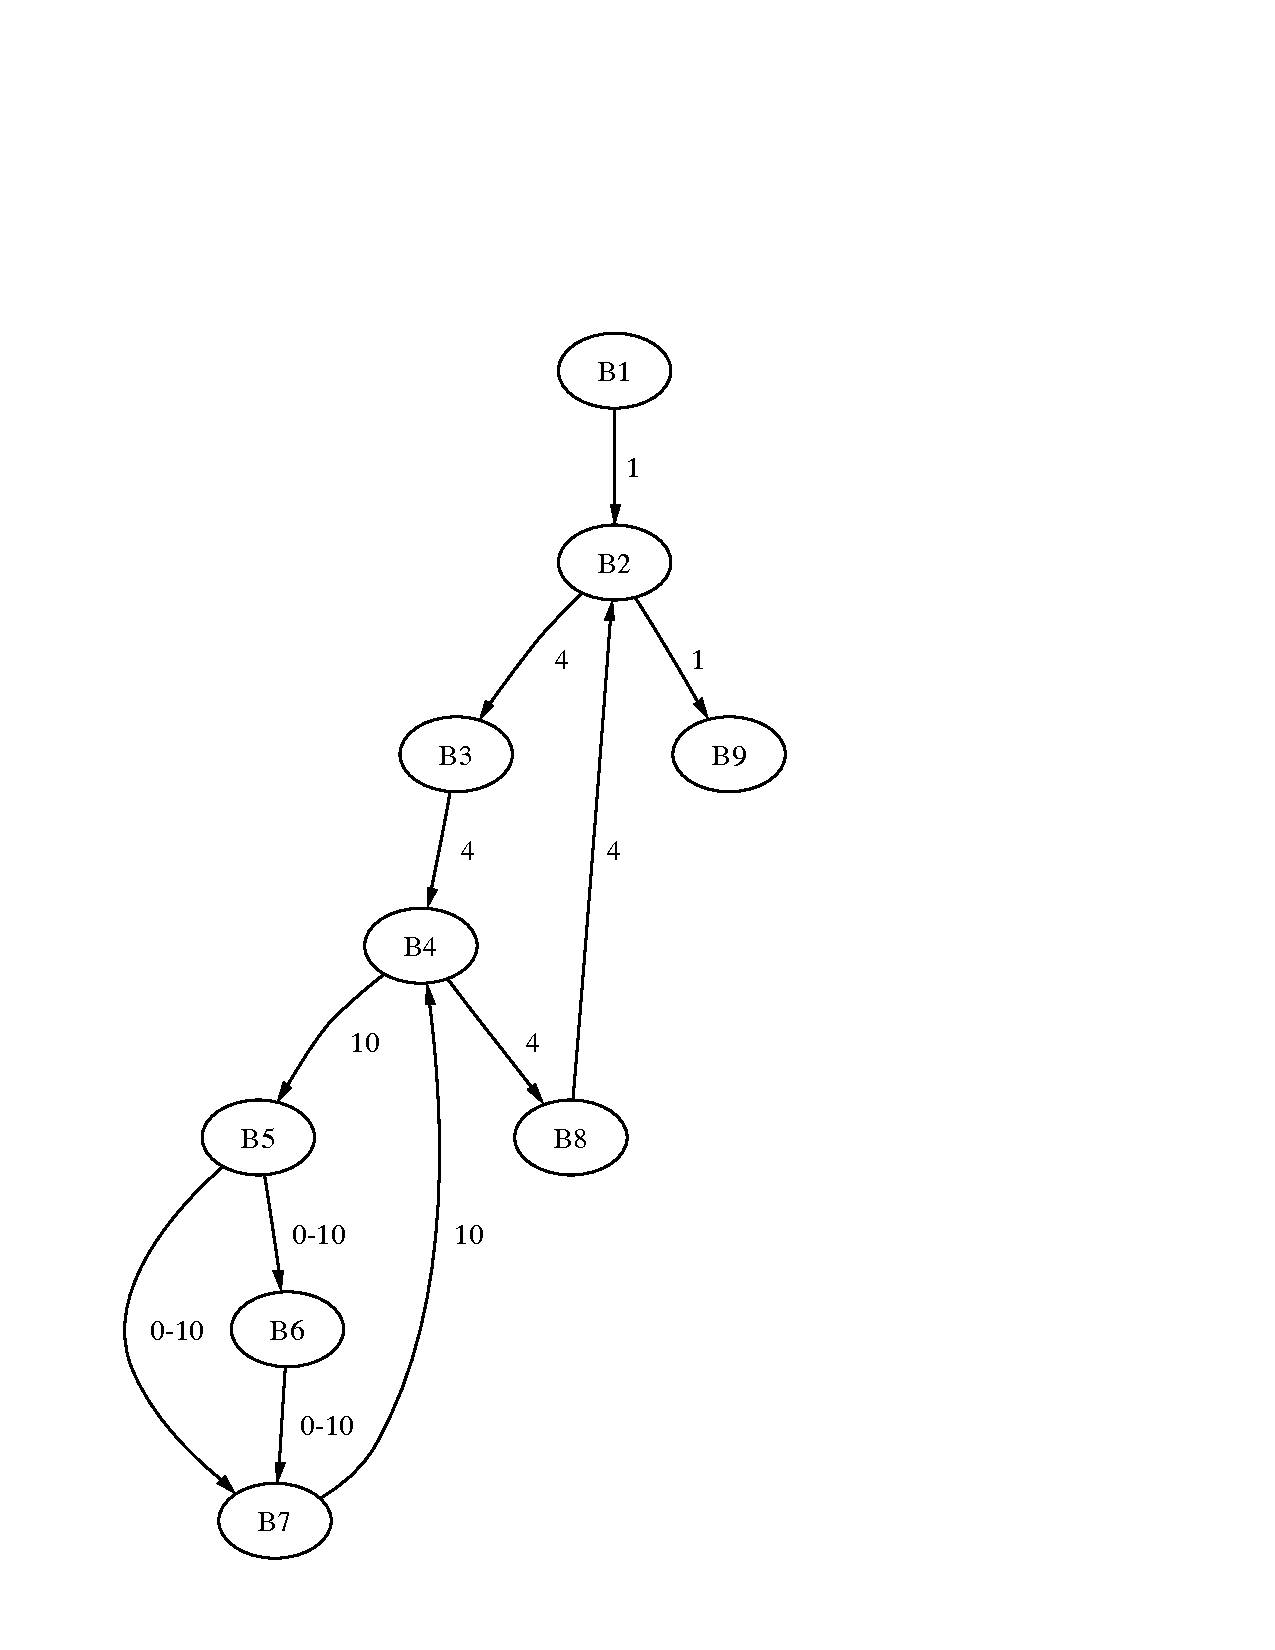
\includegraphics[height=\excelwidth]{results/results_wcet_cfg}
%    \caption{The control flow graph of the Bubble Sort example}
%    \label{fig:results:wcet:cfg}
%\end{figure}
%
%
%The values in the fifth and seventh columns (Count) of
%\tablename~\ref{tab:results:bubble:wcet} are derived from the CFG
%and show how often the basic blocks are executed in the worst and
%best cases. The WCET and BCET value for each block is calculated by
%multiplying the clock cycles by the execution frequency. The overall
%WCET and BCET values are calculated by summing the values of the
%individual blocks B1 to B8. The last block (B9) is omitted, as the
%measurement does not contain the return statement.
%
%The execution time of the program is measured using the cycle
%counter in JOP. The current time is taken at both the entry of the
%method and at the end, resulting in a measurement spanning from
%block B1 to the beginning of block B9. The last statement, the
%\code{return}, is not part of the measurement. The difference
%between these two values (less the additional 8 cycles introduced by
%the measurement itself) is given as the execution time in clock
%cycles (the last row in \tablename~\ref{tab:results:bubble:wcet}).
%The measured WCET and BCET values are exactly the same as the
%calculated values.
%
%In Figure~\ref{fig:results:wcet:sort}, the measured execution times
%for all 120 permutations of the input data are shown. The vertical
%axis shows the execution time in clock cycles and the horizontal
%axis the number of the test run. The first input sample is an
%already sorted array and results in the lowest execution time. The
%last sample is the worst-case value resulting from the reversely
%ordered input data. We can also see the 11 different execution times
%that result from executing basic block B6 (which performs the
%element exchange and takes 73 clock cycles) between 0 and 10 times.
%
%\begin{figure}
%    \centering
%    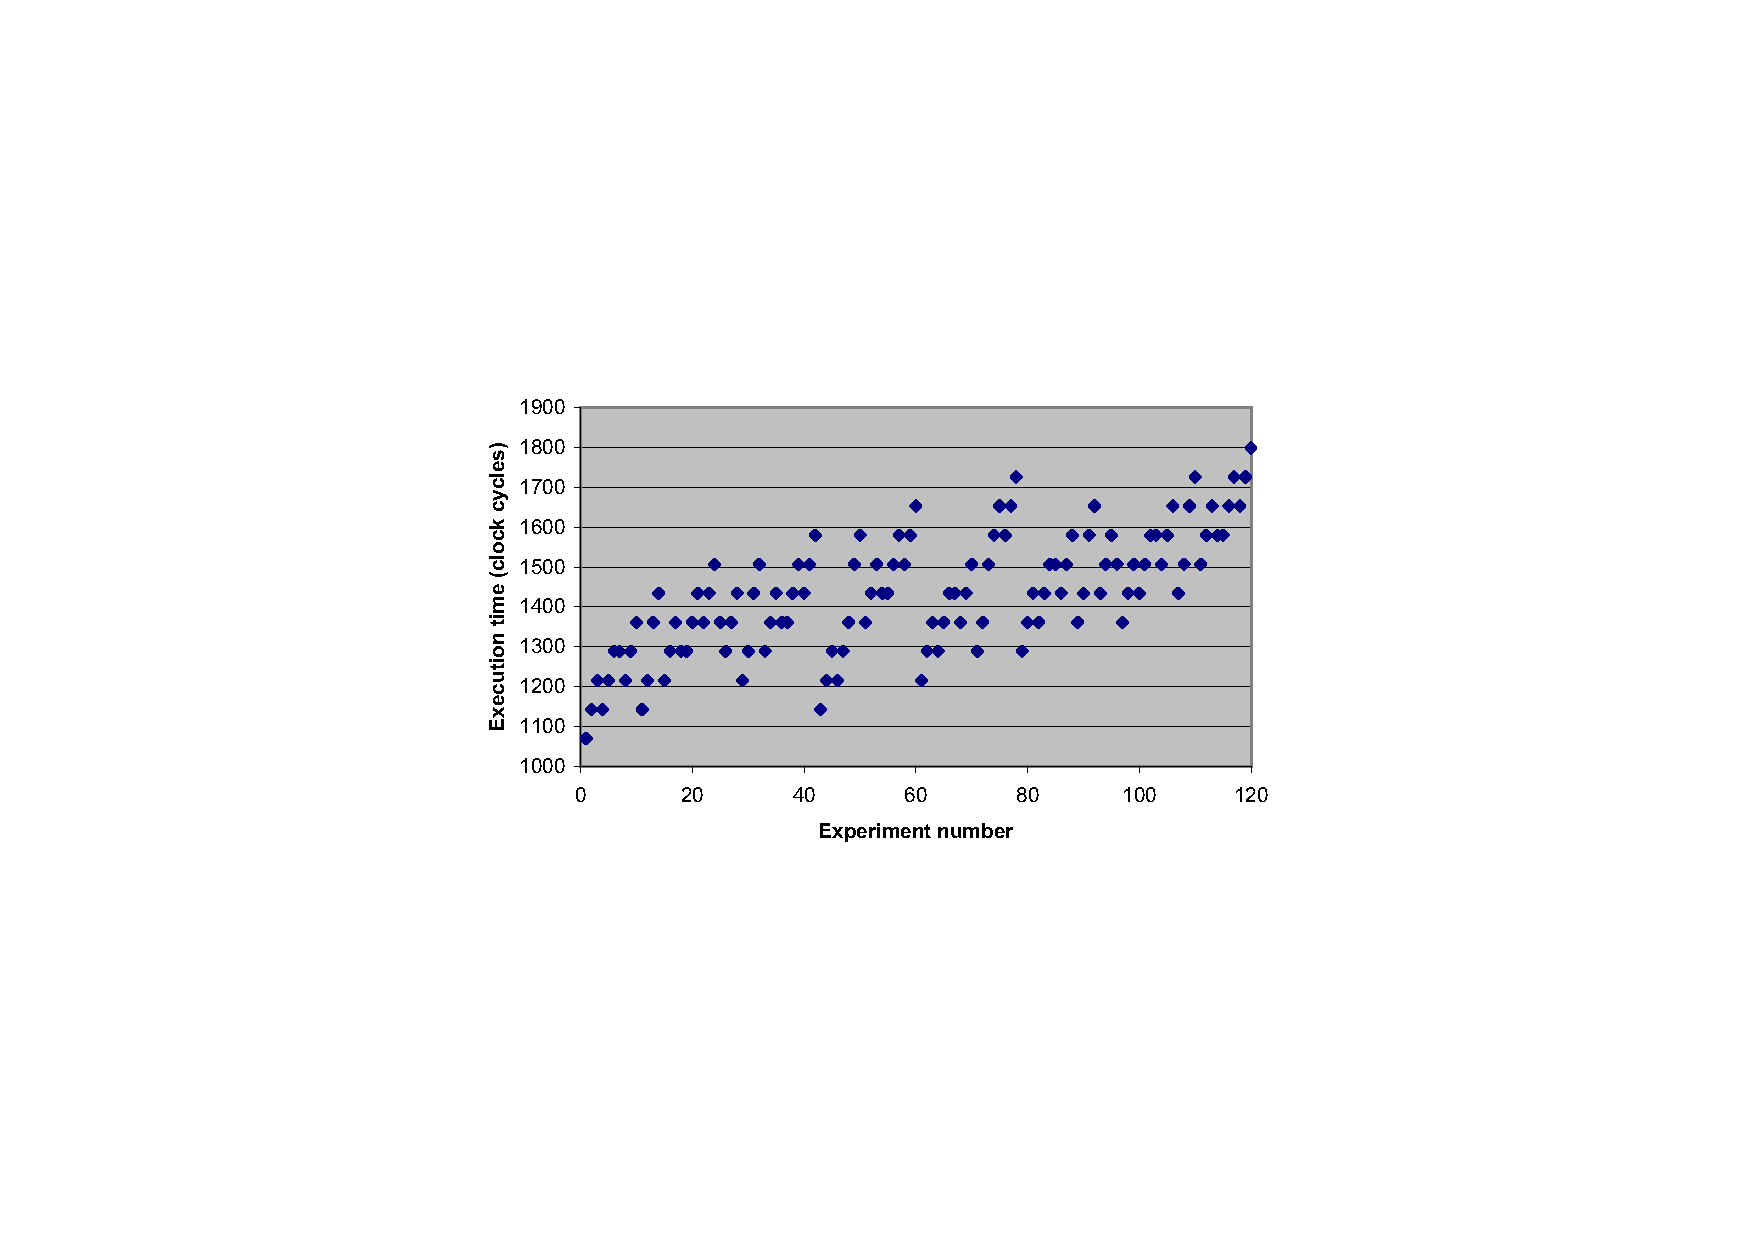
\includegraphics[width=\excelwidth]{results/results_wcet_sort}
%    \caption{Execution time in clock cycles of the Bubble Sort program}
%    \label{fig:results:wcet:sort}
%\end{figure}
%
%This example has demonstrated that JOP is a simple target for the
%WCET analysis. Most bytecodes have a single execution time (WCET =
%BCET), and the WCET of a task depends only on the control flow. No
%pipeline or data dependencies complicate the low-level part of the
%WCET analysis.
%
%%\subsection{Notes for targets}
%%
%%\subsubsection{JStamp}
%%
%%\begin{verbatim}
%%    aJile project in \usr2\ajile\bench
%%    Sources from JOP target
%%    LowLevel.java from directory aJile
%%    Remove .class in ...\dist\classes
%%    Generate .class with \bat\ajc.bat in source directory
%%        destination is ...\dist\classes
%%        e.g. in ...\src\bench: ajc jbe/DoAll
%%    aJile ChemBuilder (bench.ajp) use COM1 for System.out
%%    Terminal on Serial A, 9600 baud
%%        Did not get the System.out in Charade (but it worked some
%%        time ago)
%%    Charade: Reset, File-Load \usr2\ajile\bench\build.bin
%%\end{verbatim}


\section{Applications}
\label{sec:applications}

During the research for the PhD thesis, the first working version of
JOP was used in a real-world application. Using an architecture under
development in a commercial project entails risks. Nevertheless, this
was deemed to be the best way to prove the feasibility of the
processor. In this section, the experiences of the first project
involving JOP are summarized.

\subsection{Motor Control}
\label{sec:app:kfl}

In rail cargo, a large amount of time is spent on loading and
unloading of goods wagons. The contact wire above the wagons is the
main obstacle. Balfour Beatty Austria developed and patented a
technical solution, the so-called \emph{Kippfahrleitung}, to tilt up
the contact wire. This is done on a line up to one kilometer. An
asynchronous motor on each mast is used for this tilting. However, it
has to be done synchronously on the whole line.

Each motor is controlled by an embedded system. This system also
measures the position and communicates with a base station.
\figurename~\ref{fig:results:kfl:mast} shows the mast with the motor
and the control system in the `down' and `up' positions. The base
station has to control the deviation of individual positions during
the tilt. It also includes the user interface for the operator. In
technical terms, this is a distributed, embedded real-time control
system, communicating over an RS485 network.

\begin{figure}
    \centering
    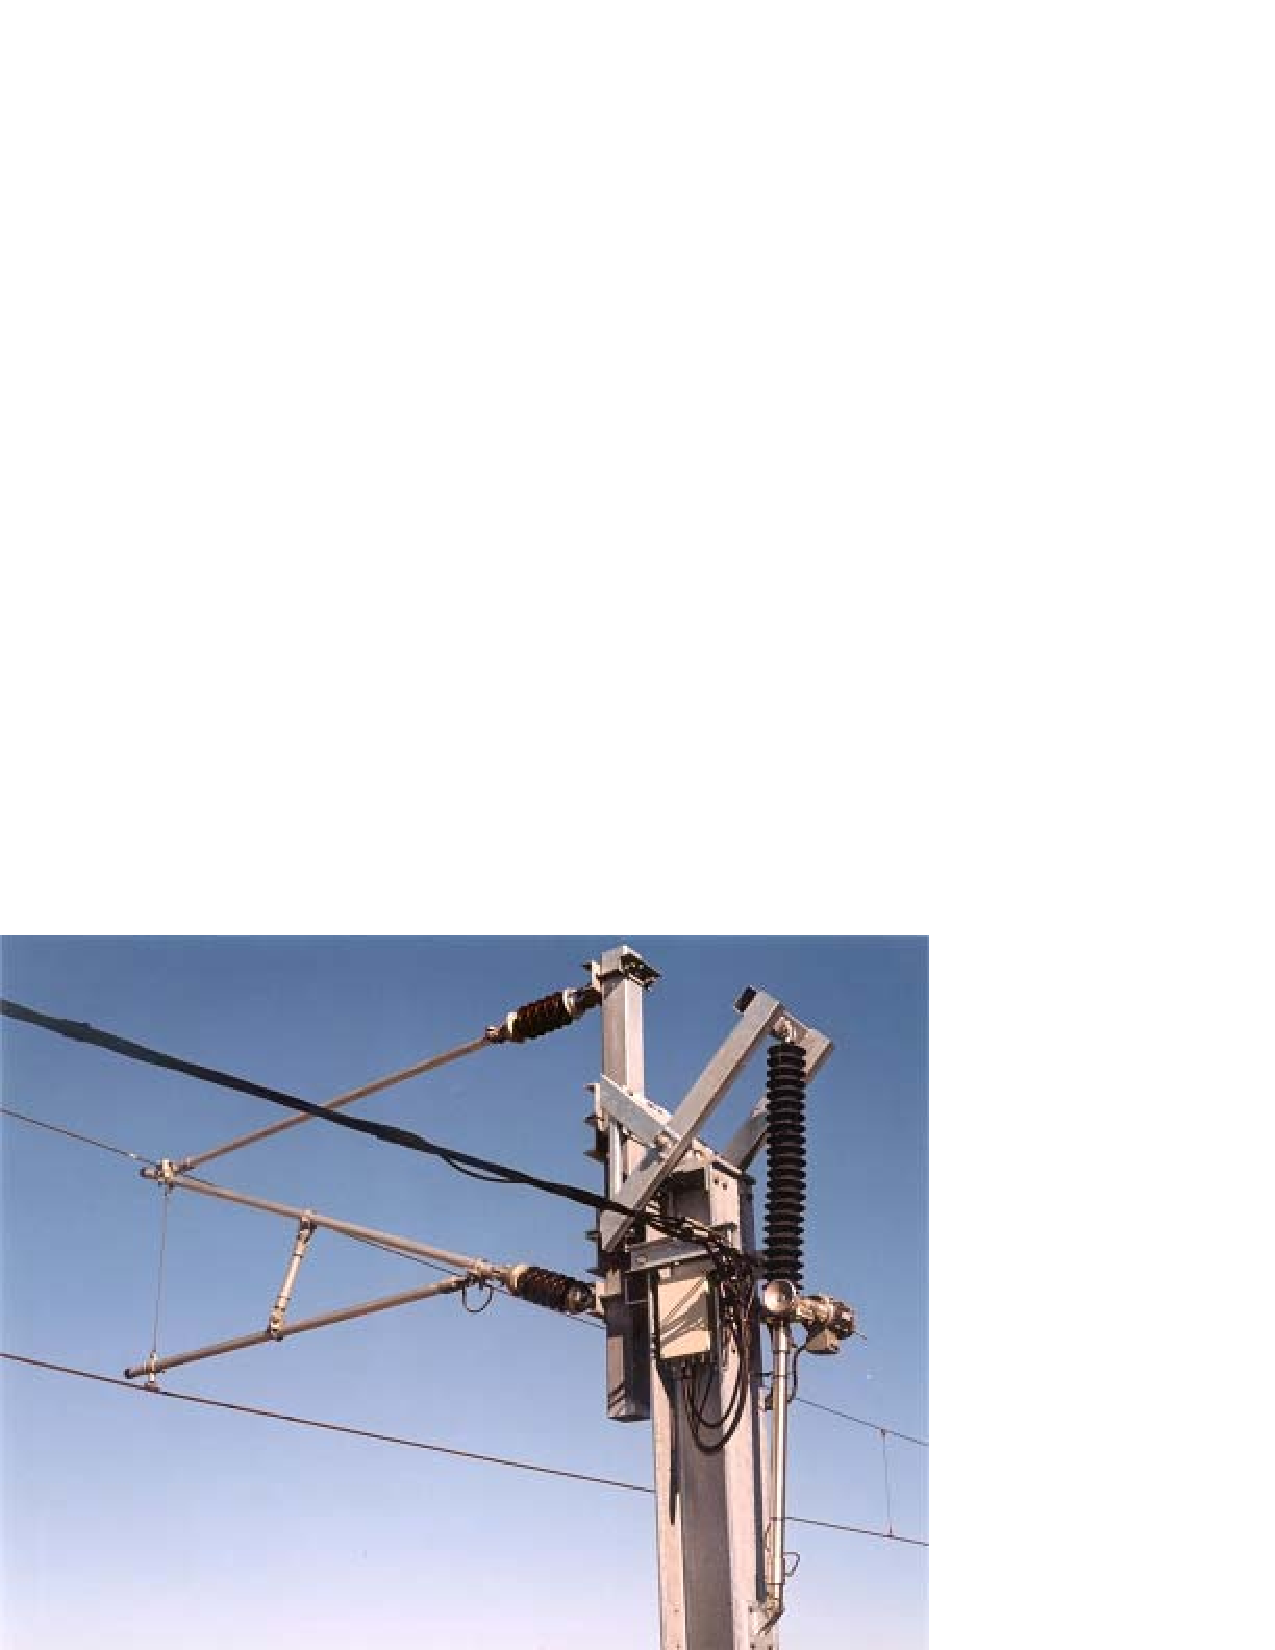
\includegraphics[width=7cm]{results/results_kfl_mast1}
    \hspace{1cm}
    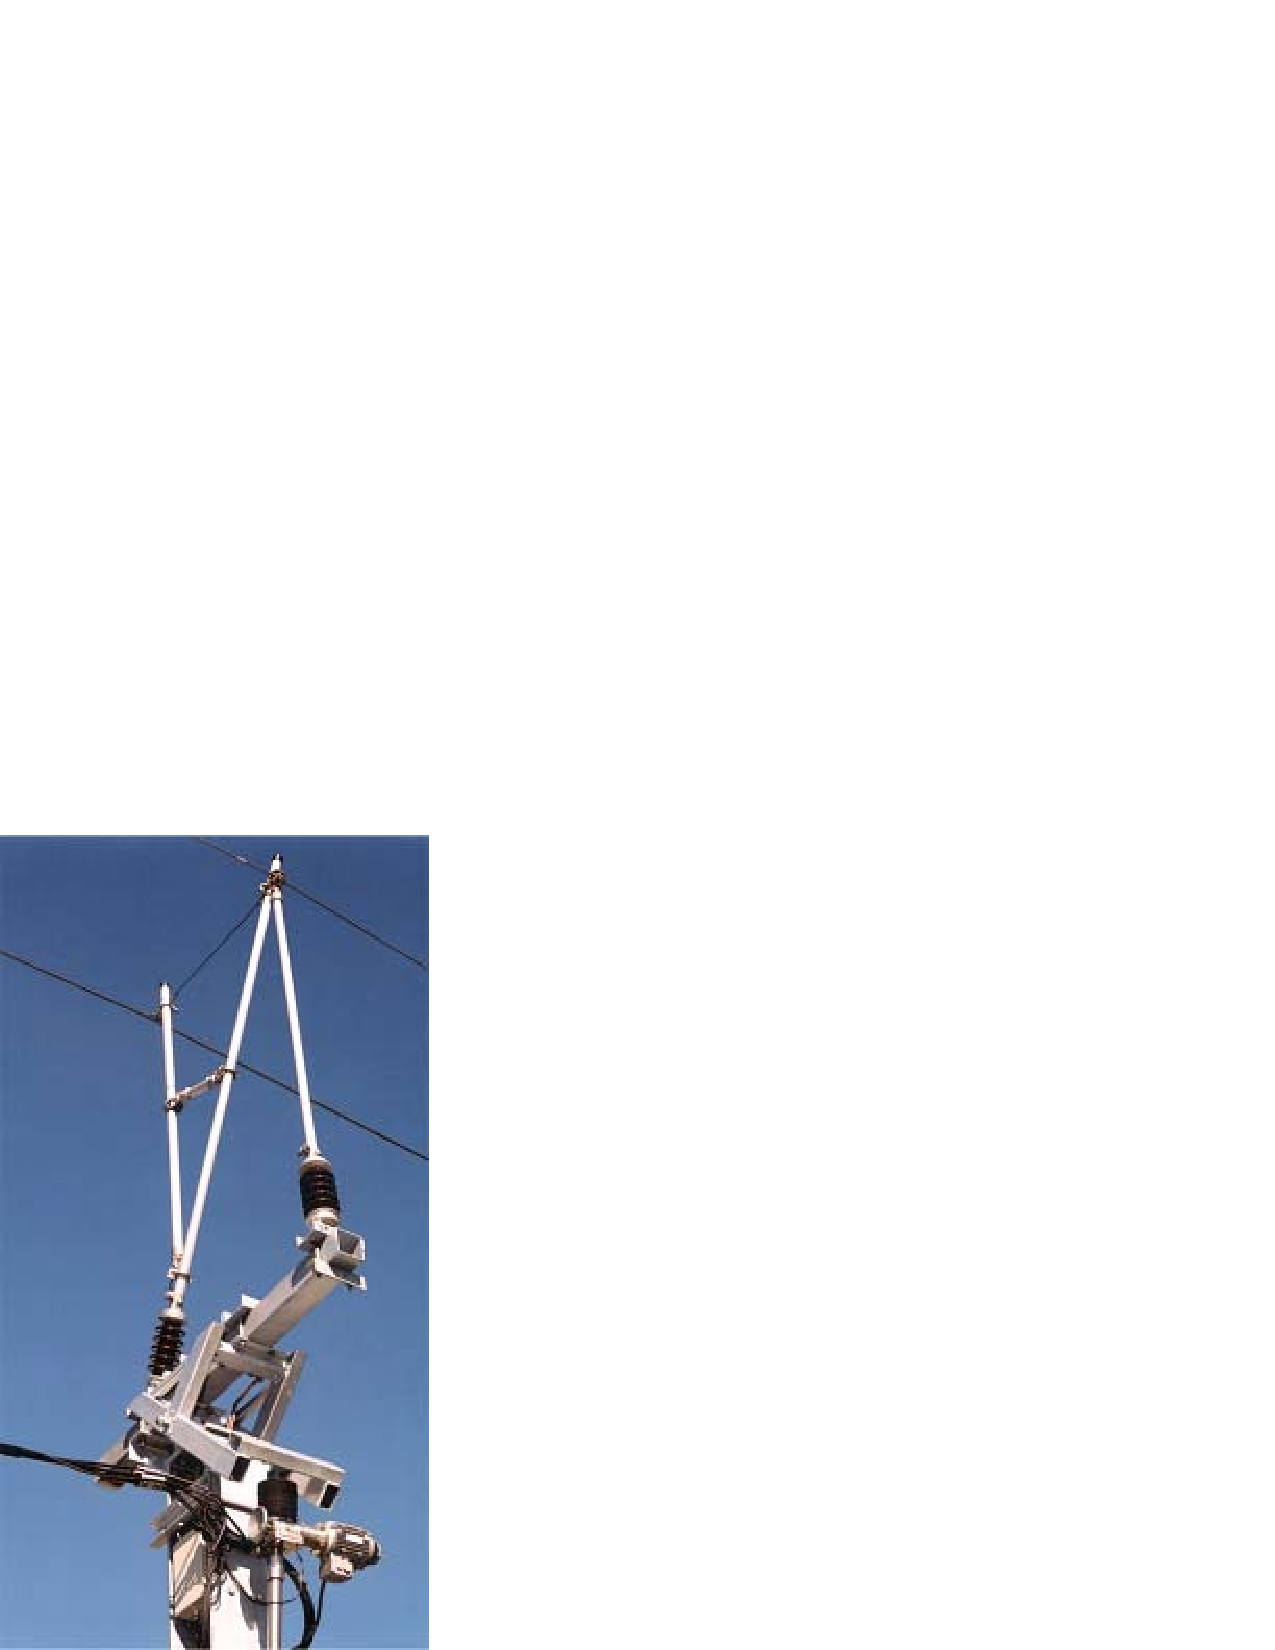
\includegraphics[width=4cm]{results/results_kfl_mast2}
    \caption{Picture of a \emph{Kippfahrleitung} mast in down and up position}
    \label{fig:results:kfl:mast}
\end{figure}

%\begin{figure}
%    \centering
%    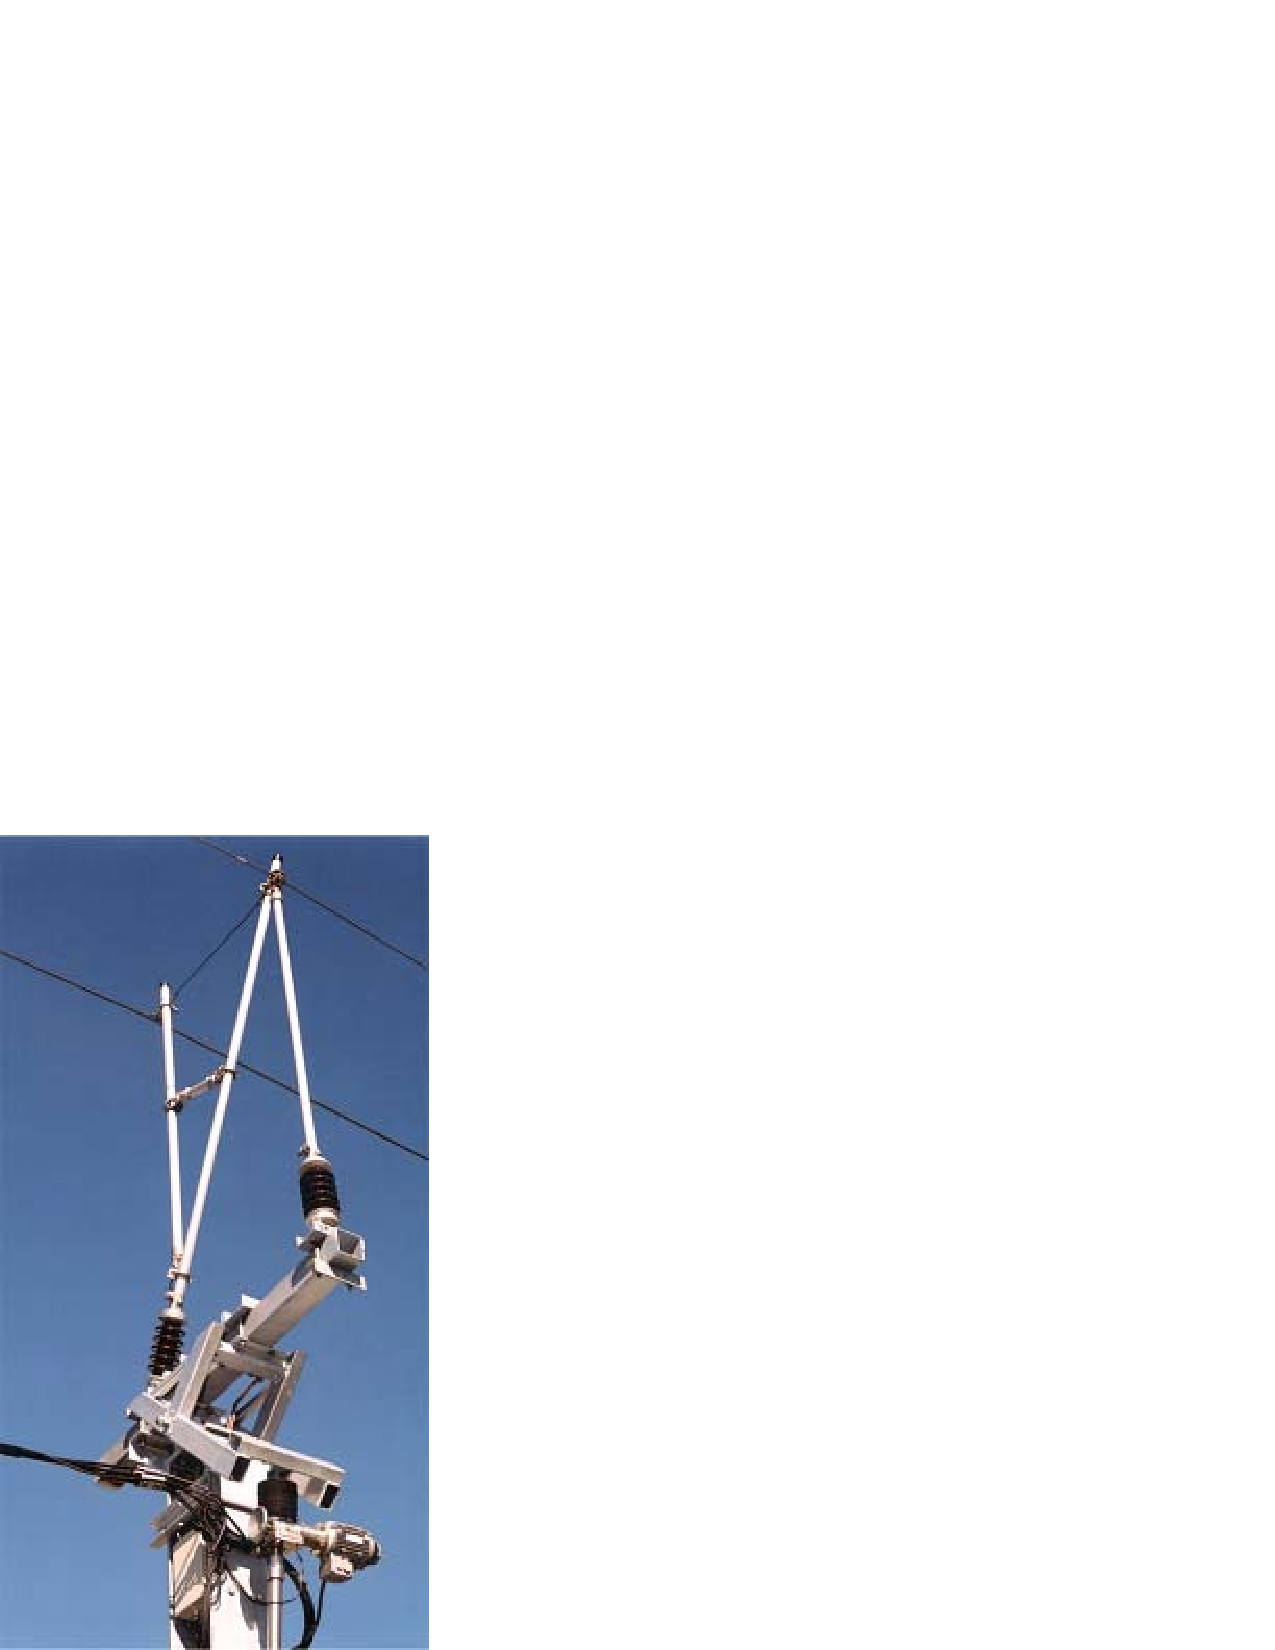
\includegraphics[width=4cm]{results/results_kfl_mast2}
%    \caption{Picture of the mast in up position}
%    \label{fig:results:kfl:mast2}
%\end{figure}


\subsubsection{Real Hardware}

Although this system is not mass-produced, there were nevertheless
cost constraints. Even a small FPGA is more expensive than a general
purpose CPU. To compensate for this, additional chips for the memory
and the FPGA configuration were optimized for cost. One standard
128KB Flash was used to hold FPGA configuration data, the Java
program and a logbook. External main memory was reduced to 128KB
with an 8-bit data bus.

To reduce external components, the boot process is a little
complicated. A watchdog circuit delivers a reset signal to a 32
macro-cell PLD. This PLD loads the configuration data into the FPGA.
When the FPGA starts, it disables the PLD and loads the Java program
from the Flash into the external RAM. After the JVM is initialized,
the program starts at \code{main()}.

The motor is controlled by silicon switches connected to the FPGA
with opto couplers. The position is measured with two end sensors and
a revolving sensor. The processor supervises the voltage and current
of the motor supply. A display and keyboard are attached to the base
station for the user interface. The communication bus (up to one
kilometer) is attached via an isolated RS485 data interface.

\subsubsection{Synthesized Hardware}

The following I/O modules were added to the JOP core in the FPGA:
%
\begin{itemize}
\item Timer
\item UART for debugging
\item UART with FIFO for the RS485 line
\item Four sigma delta ADCs
\item I/O ports
\end{itemize}
%
Five switches in the power line needed to be controlled by the
program. A wrong setting of the switches due to a software error
could result in a short circuit. Ensuring that this could not happen
was a straightforward task at the VHDL level. The sigma-delta ADCs
are used to measure the temperature of the silicon switches and the
current through the motor.

\subsubsection{Software Architecture}

The main task of the program was to measure the position using the
revolving sensor and communicate with the base station. This has to
be done under real-time constraints. This is not a very complicated
task. However, at the time of development, many features from a
full-blown JVM implementation, such as threads or objects, were
missing in JOP. The resulting Java was more like a \emph{tiny Java}.
It had to be kept in mind which Java constructs were supported by
JOP. Because there was no multi-threading capability, and in the
interests of simplicity, a simple infinite loop with constant time
intervals was used. Listing~\ref{lst:results:main} shows the
simplified program structure. After initialization and memory
allocation, this loop enters and never exits.

\begin{lstlisting}[float,caption=Simplified program structure,
label=lst:results:main]
    public static void main(String[] args) {

        init();
        Timer.start();
        forever();
        // this point is NEVER reached
    }

    private static void forever() {

        for (;;) {
            Msg.loop();
            Triac.loop();
            if (Msg.available) {
                handleMsg();
            } else {
                chkMsgTimeout();
            }
            handleWatchDog();
            Timer.waitForNextInterval();
        }
    }
\end{lstlisting}

\subsubsection{Communication}

Communication is based on a client-server structure. Only the base
station is allowed to send a request to a single mast station. The
station is then required to reply. The maximum reply time is bounded
by two time intervals. The base station handles timeout and retry. If
an irrecoverable error occurs, the base station switches off the
power to the mast stations, including the power supply to the motor.
This is the safe state of the whole system.

From the mast station perspective, every mast station supervises the
base station. The base station is required to send requests on a
regular basis. If this requirement is violated, the mast station
switches off its motor. The data is exchanged in small packets of
four bytes, including a one-byte CRC. To simplify the development,
commands to program the Flash in the mast stations and force a reset
were included. It is therefore possible to update the program, or
even change the FPGA configuration, over the network.

%\subsubsection{Benefits from using an FPGA}
%
%The flexibility of FPGAs made it possible to postpone some design
%decisions after production of the PCB. Since the production of the
%PBC was on the critical time line this helped to finish the complete
%project in time. During development, there have been situations
%where problems showed up that have not been foreseen.  Two examples
%are given where it was possible to find simple solutions:
%
%The routing of the PCB was almost finished. A question about cooling
%the switches (TRIAC) has arisen. The electronic development team
%insisted on a temperature sensor. The requirements in resolution and
%conversion time were low. A sigma-delta ADC with only two external
%passive components (a NTC thermistor and a capacitor) was
%implemented in the FPGA.
%
%When the sample rate for an ADC is low compared to the clock
%frequency of the digital system it is possible to transfer the AD
%conversion problem from the analogue to the time domain. In
%\figurename~\ref{fig_results_sigdel} the principle of a Sigma-Delta
%ADC is shown. Only the adder and the integrator have to be analogue
%components. A single bit DAC is just the FPGA digital output driving
%the signal between GND and VCCIO. The single bit ADC can be built
%with a comparator. For low resolution the threshold of the FPGA
%input is practical. The simplest form of an ADC built with an FPGA
%is shown in \figurename~\ref{fig_results_sigdel_real}. The filter
%averages $2^n$ samples and can be implemented as a counter.
%
%\begin{figure*}
%    \centering
%    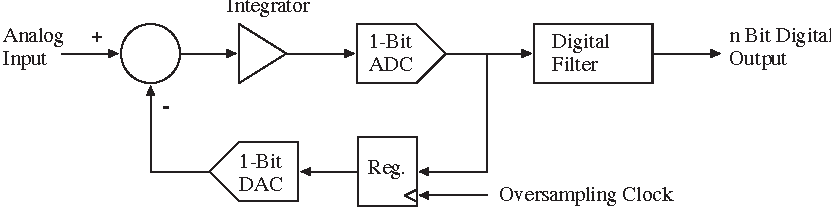
\includegraphics{results/results_sigdel}
%    \caption{A sigma-delta ADC}
%    \label{fig_results_sigdel}
%\end{figure*}
%
%
%\begin{figure*}
%    \centering
%    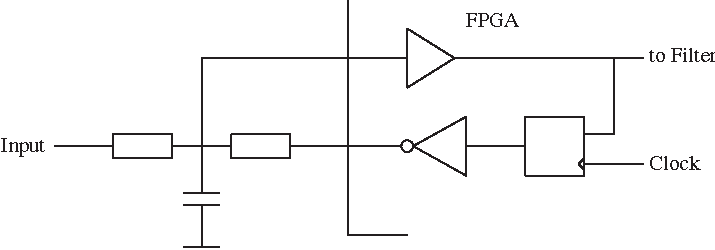
\includegraphics{results/results_sigdel_real}
%    \caption{A minimal sigma-delta ADC with an FPGA}
%    \label{fig_results_sigdel_real}
%\end{figure*}
%
%
%The AC current of the motor had to be monitored. The solution for
%this was a shunt resistor in every power line and an opto-coupler
%for isolation. However, it turned out that the shunt resistors got
%too hot and delivered to little voltage for the opto-couplers to
%work reliable. Having seen that it is possible to build an ADC in
%the FPGA a new idea was born. For EMC reasons, there is an inductor
%in every AC line. With a few windings of wire, a simple transformer
%can be built. The resulting voltage was amplified, rectified and
%used for current measurement. An additional comparator was used for
%an exacter threshold than the input buffer of the FPGA. This
%solution kept the board cool and added extra functionality. It is
%now possible to define two thresholds for too little and too much
%current.
%

\subsection{Further Projects}

TAL, short for TeleAlarm, is a remote tele-control and data logging
system. TAL communicates via a modem or an Ethernet bus with a SCADA
system or via SMS with a mobile phone. For this application, a
minimal TCP/IP stack needed to be implemented. This stack was the
reason for implementing threads and a simple real-time system in
JOP.

Another application of JOP is in a communication device with soft
real-time properties -- Austrian Railways' (\"OBB) new security
system for single-track lines. Each locomotive is equipped with a GPS
receiver and a communication device. The position of the train,
differential correction data for GPS, and commands are exchanged with
a server at the central station over a GPRS virtual private network.
JOP is the heart of the communication device in the locomotive. The
flexibility of the FPGA and an Internet connection to the embedded
system make it possible to upgrade the software and even the
processor in the field.


\section{Summary}

In this chapter, we presented an evaluation of JOP. We have seen
that JOP is the smallest hardware realization of the JVM available
to date. Due to the efficient implementation of the stack
architecture, JOP is also smaller than a \emph{comparable} RISC
processor in an FPGA. Implemented in an FPGA, JOP has the highest
clock frequency of all known Java processors.

We compared JOP against several embedded Java systems and, as a
reference, with Java on a standard PC. A Java processor is up to 500
times faster than an interpreting JVM on a standard processor for an
embedded system. JOP is about six times faster than the aJ80 Java
processor and as fast as the aJ100\footnote{The measured aJ100
system contained faster SRAMs than the FPGA board for JOP.}.
Preliminary results using compiled Java for a RISC processor in an
FPGA, with a similar resource usage and maximum clock frequency to
JOP, showed that native execution of Java bytecodes is faster than
compiled Java.

We compared the basic properties of the real-time scheduler on JOP
against the RTSJ implementation on Linux. The integration of the
scheduler in the JVM, and the timer interrupt under scheduler
control, results in an efficient platform for Java in embedded
real-time systems. JOP performs better and more predictably than the
reference implementation of the RTSJ under Linux.

We also performed WCET analysis of the implemented JVM at the
microcode level. This analysis provides the WCET and BCET values for
the individual bytecodes. We have also shown that there are no
dependencies between individual bytecodes. This feature, in
combination with the method cache (see Section~\ref{sec:cache}),
makes JOP an easy target for low-level WCET analysis of Java
applications.

Usage of JOP in three real-world applications showed that the
processor is mature enough to be used in commercial projects.


%\bibliographystyle{plain}
%\bibliography{../bib/mybib}
%\end{document}


\chapter{Related Work}
\label{chap:related}

%\emph{Update with JSA writing and remove old, not used stuff (or
%shorten it)}
    
Two different approaches can be found to improve Java bytecode
execution by hardware. The first type operates as a Java coprocessor
in conjunction with a general-purpose microprocessor. This
coprocessor is placed in the instruction fetch path of the main
processor and translates Java bytecodes to sequences of instructions
for the host CPU or directly executes basic Java bytecodes. The
complex instructions are emulated by the main processor. Java chips
in the second category replace the general-purpose CPU. All
applications therefore have to be written in Java. While the first
type enables systems with mixed code capabilities, the additional
component significantly raises costs.
\tablename~\ref{tab_related_proc} provides an overview of the
described Java hardware.

Blank fields in the table indicate that the information is not
available or not applicable (e.g. for simulation-only projects).
Minimum CPI is the number of clock cycles for a simple instruction
such as \code{nop}. One entry, the TINI system, is not a real Java
hardware, but is included in the table since it is often
incorrectly\footnote{TINI is a standard interpreting JVM running on
an enhanced 8051 processor.} cited as an embedded Java processor.


%\begin{table}
%    \centering
%{\footnotesize
%\begin{tabular}
%    {|>{\bfseries}p{1.4cm}|m{1.3cm}|>{\raggedright}m{1.3cm}|>{\raggedright}m{1.3cm}
%    |r|>{\raggedright}m{1.35cm}|r|m{1.6cm}|}
%
%    \hline
%         & Type & Target  & Size & Speed & Java     & Min. & Remarks \\
%         &      & technology &      & [MHz] & standard & CPI  &         \\
%    \hline
%    Hard-Int & Translation & Simulation only &  &  &  &  &  \\
%    \hline
%    DELFT & Translation & Simulation only &  &  &  &  &  \\
%    \hline
%    JIFFY & Translation & Xilinx FPGA & 3800 LCs, 1KB RAM &  &  &  &  \\
%    \hline
%    Jazelle & Co-processor & ASIC 0.18$\mu$ & 12K gates & 200 &  &  & Integration with ARM \\
%    \hline
%    JSTAR & Co-processor & ASIC 0.18$\mu$ Softcore & 30K gates + 7KB & 104 & J2ME CLDC\footnotemark[2] &  &  \\
%    \hline
%    TINI & Software JVM & Enhanced 8051 clone &  &  & Java 1.1 subset &  & A small Java system for embedded applications. \\
%    \hline
%    picoJava & Processor & No realization & 128K gates + memory &  & Full & 1 &  \\
%    \hline
%    aJile & Processor & ASIC 0.25$\mu$ & 25K gates + ROM & 100 & J2ME CLDC\footnotemark[2] &  &  \\
%    \hline
%    Cjip & Processor & ASIC 0.35$\mu$ & 70K gates + ROM, RAM & 67 & J2ME CLDC\footnotemark[2] & 6 & Rewriteable microcode \\
%    \hline
%    Ignite & Stack processor & Xilinx FPGA & 9700 LCs &  &  &  &  \\
%    \hline
%    Moon & Processor & Altera FPGA & 3660 LCs, 4KB RAM &  &  &  &  \\
%    \hline
%    Lightfoot & Processor & Xilinx FPGA & 3400 LCs & 40 &  &  &  \\
%    \hline
%    LavaCORE & Processor & Xilinx FPGA & 3800 LCs 30K gates & 20 &  &  &  \\
%    \hline
%    Komodo & Processor & Xilinx FPGA & 2600 LCs & 20 & Subset: 50 bytecodes & 4 &  \\
%    \hline
%    FemtoJava & Processor & Altera Flex 10K & 2000 LCs & 4 & Subset: 69 bytecodes, 16-bit ALU & 3 & Application specific Java processor. \\
%    \hline
%    JSM & Processor & Xilinx FPGA &  & 3.5 & Java Card &  & \cite{JSM01} \\
%    \hline
%%    \hline
%%    JOP & Processor & Altera, Xilinx FPGA & 2100 LCs + 3KB RAM & 100 & J2ME CLDC & 1 & Typical configuration on a Cyclone FPGA \\
%
%\end{tabular}
%}
%    \caption{Java hardware}
%    \label{tab_related_proc}
%\end{table}


\begin{table}
    \centering
{\footnotesize
\begin{tabular}
    {|>{\bfseries}p{1.6cm}|m{1.5cm}|>{\raggedright}m{1.6cm}|>{\raggedright}m{1.6cm}
    |r|>{\raggedright}m{1.5cm}|r|}

    \hline
         & Type & Target  & Size & Speed & Java     & Min. \\
         &      & technology &      & [MHz] & standard & CPI  \\
    \hline
    Hard-Int & Translation & Simulation only &  &  &  &  \\
    \hline
    DELFT & Translation & Simulation only &  &  &  &    \\
    \hline
    JIFFY & Translation & Xilinx FPGA & 3800 LCs, 1KB RAM &  &  &   \\
    \hline
    Jazelle & Co-processor & ASIC 0.18$\mu$ & 12K gates & 200 &  &  \\
    \hline
    JSTAR & Co-processor & ASIC 0.18$\mu$ Softcore & 30K gates + 7KB & 104 & J2ME CLDC\footnotemark[2] &  \\
    \hline
    TINI & Software JVM & Enhanced 8051 clone &  &  & Java 1.1 subset &   \\
    \hline
    picoJava & Processor & No realization & 128K gates + memory &  & Full & 1  \\
    \hline
    aJile & Processor & ASIC 0.25$\mu$ & 25K gates + ROM & 100 & J2ME CLDC\footnotemark[2] &   \\
    \hline
    Cjip & Processor & ASIC 0.35$\mu$ & 70K gates + ROM, RAM & 67 & J2ME CLDC\footnotemark[2] & 6 \\
    \hline
    Ignite & Stack processor & Xilinx FPGA & 9700 LCs &  &  &   \\
    \hline
    Moon & Processor & Altera FPGA & 3660 LCs, 4KB RAM &  &  &   \\
    \hline
    Lightfoot & Processor & Xilinx FPGA & 3400 LCs & 40 &  &   \\
    \hline
    LavaCORE & Processor & Xilinx FPGA & 3800 LCs 30K gates & 20 &  &   \\
    \hline
    Komodo & Processor & Xilinx FPGA & 2600 LCs & 20 & Subset: 50 bytecodes & 4  \\
    \hline
    FemtoJava & Processor & Altera Flex 10K & 2000 LCs & 4 & Subset: 69 bytecodes, 16-bit ALU & 3 \\
    \hline
    JSM \cite{JSM01} & Processor & Xilinx FPGA &  & 3.5 & Java Card &   \\
    \hline
%    \hline
%    JOP & Processor & Altera, Xilinx FPGA & 2100 LCs + 3KB RAM & 100 & J2ME CLDC & 1 & Typical configuration on a Cyclone FPGA \\

\end{tabular}
}
    \caption{Java hardware}
    \label{tab_related_proc}
\end{table}

\footnotetext[2]{J2ME CLDC stands for Java2 Micro Edition, Connected
Limited Device Configuration, which is described in
Section~\ref{subsec:cldc}.}


% Change this: \emph{JOP is included with a typical configuration as a
% reference. Further details of the resource usage of JOP is described
% in Section~xxx.}


\section{Hardware Translation and Coprocessors}

The simplest enhancement for Java is a translation unit, which
substitutes the switch statement of an interpreter JVM (bytecode
decoding) through hardware and/or translates simple bytecodes
to a sequence of RISC instructions on the fly.

A standard JVM interpreter contains a loop with a large switch
statement that decodes the bytecode (see
Listing~\ref{lst:intro:java:intprt}). This switch statement is
compiled to an indirect branch. The destinations of these indirect
branches change frequently and do not benefit from branch-prediction
logic. This is the main overhead for simple bytecodes on modern
processors. The following approaches enhance the execution of Java
programs on a standard processor through the substitution of the
memory read and switch statement with bytecode fetch and decode
through hardware.


\subsection{Hard-Int}

Radhakrichnan \cite{HardInt} proposes an additional architecture for
a standard RISC processor to speed up a JVM interpreter. The
architecture, called Hard-Int, is placed between the cache and
instruction fetch of the RISC processor. Simple Java bytecodes are
translated to a sequence of RISC instructions. For native RISC code,
the unit is bypassed. This architecture implements the expensive
switch statement of a typical interpreter in hardware. A simulation
of a SPARC processor with four execution units shows a speedup by
the factor of 2.6 over JDK 1.2 JIT with SPECjvm98. Since the
architecture is only evaluated in a software simulation, the impact
of the inserted hardware on the clock frequency of the RISC
processor is unknown. No estimation of the additional hardware cost
for the translation unit is given.


\subsection{DELFT-JAVA Engine}

In his thesis \cite{DELFT}, Glossner describes a processor for
multimedia applications in Java. A RISC processor is extended with
DSP capabilities and Java specific instructions. This combination
results in a very complex processor. Simple JVM instructions are
dynamically translated to the DELFT instruction set. However, no
explanation is given as to how this is done. A new
register-addressing mode, indirect register addressing with auto
increment or decrement, provides support for stack caching in the
register file. The translation of JVM bytecode to the DELFT
instruction set maps stack-based dependencies into pipeline
dependencies. The author expects that these dependencies can be
resolved with standard techniques such as register renaming and
out-of-order execution. To accelerate dynamic linking a link
translation buffer cache resolved entries from the constant pool.


The processor is validated through a C++ model. An experiment with a
synthetic benchmark (vector multiplication) compared a stack machine
with an ideal register machine. The ideal register machine performs
register renaming and out-of-order execution on multiple execution
units. The achieved speedup in this experiment was 2.7. The
high-level simulation model is more a proof of concept and no
estimation is given for the resources needed to implement this
complex processor. Since only a restricted subset of the JVM was
simulated, no Java applications could be used to estimate the
expected speedup.


\subsection{JIFFY}

An interesting approach to enhance Java execution in embedded
systems is presented in Acher's thesis \cite{JIFFY}. He states that
JIT-compilation in software is not possible on most embedded devices
because of resource constraints. JIFFY, a JIT in an FPGA, is
proposed as a solution to this problem. The compilation is done in
the following steps:

The Java bytecode is translated into an intermediate language with
three registers and a stack. The reduction to three registers is due
to the fact that bytecodes are using a maximum of three stack
operands, and it simplifies translation to CISC-architectures with a
low register count. In the next step, this instruction sequence,
which is still stack-based, is optimized. The main effect of this
optimization is to transform stack-based operations into
register-based operations. These optimized instructions in the
intermediate language are translated to native instructions of the
target architecture in the last step.

The quality of the generated code was tested with software versions
of JIFFY for a CISC (80586) and a RISC (Alpha 21164) architecture.
The resulting code is about 1.1 to 7.5 times faster than
interpreting Java bytecode on the x86 architecture. The speedup is
similar to Suns first JIT compiler (sunwjit in JDK 1.1). The
compilation time is estimated to be 50 to 70 clock cycles for one
bytecode. This is 10 times faster than the efficient CACAO JIT
\cite{Krall98}. A first prototype implementation in an FPGA used
3800 LCs and 8KBits RAM (80 \% of a Xilinx XC2S200).


\subsection{Jazelle}

Jazelle \cite{Jazelle} is an extension of the ARM 32-bit RISC
processor, similar to the Thumb state (a 16-bit mode for reduced
memory consumption). The Jazelle coprocessor is integrated into the
same chip as the ARM processor. The hardware bytecode decoder logic
is implemented in less than 12K gates. It accelerates, according to
ARM, some 95\% of the executed bytecodes. 140 bytecodes are executed
directly in hardware, while the remaining 94 are emulated by
sequences of ARM instructions. This solution also uses code
modification with \textit{quick} instructions to substitute certain
object-related instructions after link resolution. All Java
bytecodes, including the emulated sequences, are re-startable to
enable a fast interrupt response time.


A new ARM instruction puts the processor into Java state. Bytecodes
are fetched and decoded in two stages, compared to a single stage in
ARM state. Four registers of the ARM core are used to cache the top
stack elements. Stack spill and fill is handled automatically by the
hardware. Additional registers are reused for the Java stack
pointer, the variable pointer, the constant pool pointer and locale
variable 0 (the \textit{this} pointer in methods). Keeping the
complete state of the Java mode in ARM registers simplifies its
integration into existing operating systems.

\subsection{JSTAR, JA108}

Nozomi's JA108 \cite{JSTAR}, previously known as JSTAR, Java
coprocessor sits between the native processor and the memory
subsystem. JA108 fetches Java bytecodes from memory and translates
them into native microprocessor instructions. JA108 acts as a
pass-through when the core processor's native instructions are being
executed. The JA108 is targeted for use in mobile phones to increase
performance of Java multimedia applications. The coprocessor is
available as standalone package or with included memory and can be
operated up to 104MHz. The resource usage for the JSTAR is known to
be about 30K gates plus 45Kbits for the microcode.

\subsection{A Co-Designed Virtual Machine}

In his thesis \cite{KentPhD}, Kent proposes an interesting new form
of Java coprocessor. He investigates hardware/software co-design for
a JVM within the context of a desktop workstation. The execution of
the JVM is partitioned between an FPGA and the host processor. An
FPGA board with local memory is connected via the PCI bus to the
host. This solution provides an add-on accelerator without changing
the system. Moreover, as the FPGA can be configured for a different
task, the add-on hardware can be used for non-Java applications.

The critical issue in this approach is the partitioning of the JVM
and the memory regions between hardware and software. Not all Java
bytecodes can be executed in hardware. All object-oriented bytecodes
are performed in software. However, once these bytecodes are
replaced by their \textit{quick} variants, some of them can then be
executed in hardware. The most accessed data structures, i.e.\ the
method's bytecode, execution stack and local variables, are placed
in the FPGA board memory. The constant pool and the heap reside in
the PC's main memory. The software part of the JVM decides during
runtime which instruction sequences can be executed by the hardware.
Due to the high cost of a context switch, this is a critical
decision. Kent explored various algorithms with different block
sizes to find the optimum partitioning of the instructions between
the host processor and the FPGA. Tests with small benchmarks on a
simulation showed performance gains by a factor of 6 to 11, when
compared with an interpreting JVM. Kent is now working on the
concurrent use of the FPGA and the host system to execute Java
applications. Additional performance increases are expected for
multi-threaded applications.

In our view, there are two potential problems with this approach.
Firstly, the execution context for the hardware is too small. As
\code{invokevirtual} and the quick version are implemented in the
software partition, the maximum context is one method body. As shown
in Section~\ref{sec:bench:jvm:methods}, Java methods are usually
small (about 30\% are less than 9 bytes long), resulting in many
context switches. The second issue is the raw speedup, without
communication overhead, of the FPGA solution. This speedup is stated
to be around of 10 times greater, with the same clock frequency.
However, FPGA clock rate will never reach the clock rate of a
general-purpose processor. With a meaningful design, such as a CPU,
the clock rate of an FPGA is about 20 to 50 times lower. However,
everyone who uses an FPGA as target technology for a processor
design faces this problem. It is better not to try to compete
against mainstream PC technology.

\section{Java Processors}

Java Processors are primarily used in an embedded system. In such a
system, Java is the native programming language and all operating
system related code, such as device drivers, are implemented in
Java. Java processors are simple or extended stack architectures
with an instruction set that resembles more or less the bytecodes
from the JVM.

\subsection{picoJava}
\label{subsec:related:picojava}

Sun's picoJava is the Java processor most often cited in research
papers. It is used as a reference for new Java processors and as the
basis for research into improving various aspects of a Java
processor. Ironically, this processor was never released as a
product by Sun. After Sun decided to not produce picoJava in
silicon, Sun licensed picoJava to Fujitsu, IBM, LG Semicon and NEC.
However, these companies also did not produce a chip and Sun finally
provided the full Verilog code under an open-source license.

Sun introduced the first version of picoJava \cite{624084} in 1997.
The processor was targeted at the embedded systems market as a pure
Java processor with restricted support of C. picoJava-I contains
four pipeline stages. A redesign followed in 1999, known as
picoJava-II. This is the version described below. picoJava-II is now
freely available with a rich set of documentation \cite{pjMicroArch,
pjProgRef}.

Simple Java bytecodes are directly implemented in hardware, most of
them execute in one to three cycles. Other performance critical
instructions, for instance invoking a method, are implemented in
microcode. picoJava traps on the remaining complex instructions,
such as creation of an object, and emulates this instruction. To
access memory, internal registers and for cache management picoJava
implements 115 extended instructions with 2-byte opcodes. These
instructions are necessary to write system-level code to support the
JVM.

Traps are generated on interrupts, exceptions and for instruction
emulation. A trap is rather expensive and has a minimum overhead of
16 clock cycles:

\begin{verbatim}
    6 clocks trap execution
    n clocks trap code
    2 clocks set VARS register
    8 clocks return from trap
\end{verbatim}


This minimum value can only be achieved if the trap table entry is
in the data cache and the first instruction of the trap routine is
in the instruction cache. The worst-case interrupt latency is 926
clock cycles \cite{pjProgRef}.

\begin{figure*}
    \centering
%    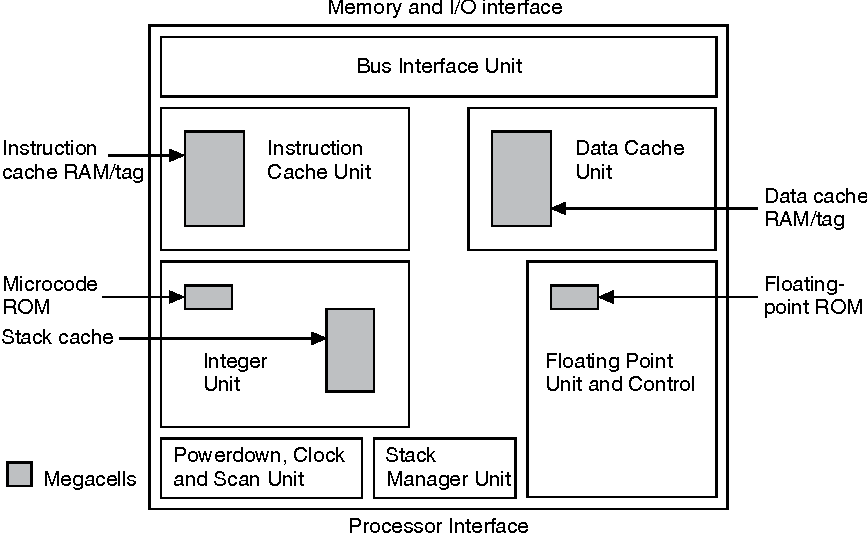
\includegraphics[scale=\picscale]{related/related_picojava}
    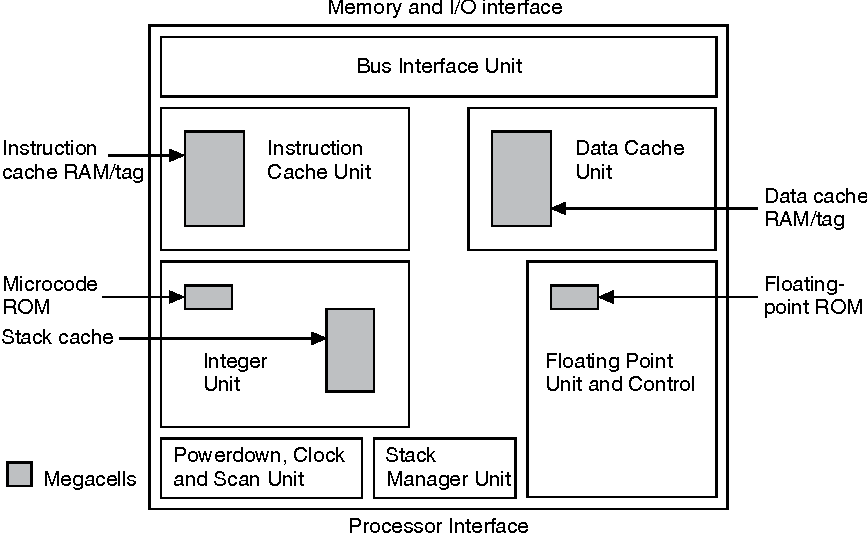
\includegraphics[scale=0.85]{related/related_picojava}
    \caption[Block diagram of picoJava-II]
    {Block diagram of picoJava-II (from \cite{pjMicroArch})}
    \label{fig_related_picojava}
\end{figure*}

\figurename~\ref{fig_related_picojava} shows the major function
units of picoJava. The integer unit decodes and executes picoJava
instructions. The instruction cache is direct-mapped, while the data
cache is two-way set-associative, both with a line size of 16 bytes.
The caches can be configured between 0 and 16 Kbytes. An instruction
buffer decouples the instruction cache from the decode unit. The FPU
is organized as a microcode engine with a 32-bit datapath supporting
single- and double-precision operations. Most single-precision
operations require four cycles. Double-precision operations require
four times the number of cycles as single-precision operations. For
low-cost designs, the FPU can be removed and the core traps on
floating-point instructions to a software routine to emulate these
instructions. picoJava provides a 64-entry stack cache as a register
file. The core manages this register file as a circular buffer, with
a pointer to the top of stack. The stack management unit
automatically performs spill to and fill from the data cache to
avoid overflow and underflow of the stack buffer. To provide this
functionality the register file contains five memory ports.
Computation needs two read ports and one write port, the concurrent
spill and fill operations the two additional read and write ports.
The processor core consists of following six pipeline stages:
%
\begin{description}

\item[Fetch:]
Fetch 8 bytes from the instruction cache or 4 bytes from the bus
interface to the 16-byte-deep prefetch buffer.

\item[Decode:]
Group and precode instructions (up to 7 bytes) from the prefetch
buffer. Instruction folding is performed on up to four bytecodes.

\item[Register:]
Read up to two operands from the register file (stack cache).

\item[Execute:]
Execute simple instructions in one cycle or microcode for
multi-cycle instructions.

\item[Cache:]
Access the data cache.

\item[Writeback:]
Write the result back into the register file.

\end{description}
%
The integer unit together with the stack unit provides a mechanism,
called instruction folding, to speed up common code patterns found
in stack architectures, as shown in
\figurename~\ref{fig_related_folding}.
%
\begin{figure}
A Java instruction
    \begin{verbatim}
    c = a + b;
    \end{verbatim}
translates to the following bytecodes:
    \begin{verbatim}
    iload_1
    iload_2
    iadd
    istore_3
    \end{verbatim}
    \caption{A common folding pattern that is executed in a single cycle}
    \label{fig_related_folding}
\end{figure}
%
When all entries are contained in the stack cache, the picoJava core
can fold these four instructions to one RISC-style single cycle
operation.

picoJava contains a simple mechanism to speed-up the common case for
monitor enter and exit. The two low order bits of an object
reference are used to indicate the lock holding or a request to a
lock held by another thread. These bits are examined by
\code{monitorenter} and \code{monitorexit}. For all other operations
on the reference, these two bits are masked out by the hardware.
Hardware registers cache up to two locks held by a single thread.

To efficiently implement a generational or an incremental garbage
collector picoJava offers hardware support for write barriers
through memory segments. The hardware checks all stores of an object
reference if this reference points to a different segment (compared
to the store address). In this case, a trap is generated and the
garbage collector can take the appropriate action. Additional two
reserved bits in the object reference can be used for a write
barrier trap.

The architecture of picoJava is a stack-based CISC processor
implementing 341 different instructions \cite{pJ1} and is the most
complex Java processor available. The processor can be implemented
\cite{Sekar2000} in about 440K gates (128K for the logic and 314K
for the memory components: 284x80 bits microcode ROM, 2x192x64 bits
FPU ROM and 2x16~KB caches). We have implemented picoJava-II in a
Cyclone-II FPGA \cite{pjfpga} and the design consumed 27500~LCs and
48~KB on-chip memory.

\subsection{aJile JEMCore}

aJile's JEMCore is a direct-execution Java processor that is
available as both an IP core and a stand alone processor
\cite{aJile, 880720}. It is based on the 32-bit JEM2 Java chip
developed by Rockwell-Collins. JEM2 is an enhanced version of JEM1,
created in 1997 by the Rockwell-Collins Advanced Architecture
Microprocessor group. Rockwell-Collins originally developed JEM for
avionics applications by adapting an existing design for a
stack-based embedded processor. Rockwell-Collins decided not to sell
the chip on the open market. Instead, it licensed the design
exclusively to aJile Systems Inc., which was founded in 1999 by
engineers from Rockwell-Collins, Centaur Technologies, Sun
Microsystems, and IDT.


The core contains 24 32-bit wide registers. Six of them are used to
cache the top elements of the stack. The datapath consists of a
32-bit ALU, a 32-bit barrel shifter and the support for floating
point operations (disassembly/assembly, overflow and NaN detection).
The control store is a 4K by 56 ROM to hold the microcode that
implements the Java bytecode. An additional RAM control store can be
used for custom instructions. This feature is used to implement the
basic synchronization and thread scheduling routines in microcode.
This results in low execution overheads with thread-to-thread yield
of less than one $\mu$s (at 100MHz). An optional Multiple JVM
Manager (MJM) supports two independent, memory protected JVMs. The
two JVMs execute time-sliced on the processor. According to aJile,
the processor can be implemented in 25K gates (without the microcode
ROM). The MJM needs additional 10K gates.

Two silicon versions of JEM exist today: the aJ-80 and the aJ-100.
Both versions comprise a JEM2 core, the MJM, 48KB zero wait state
RAM and peripheral components, such as timer and UART. 16KB of the
RAM is used for the writable control store. The remaining 32KB is
used for storage of the processor stack. The aJ-100 provides a
generic 8-bit, 16-bit or 32-bit external bus interface, while the
aJ-80 only provides an 8-bit interface. The aJ-100 can be clocked up
to 100MHz and the aJ-80 up to 66MHz. The power consumption is about
1mW per MHz.

Since aJile was a member of the Real-Time for Java Expert Group, the
complete RTSJ will be available in the near future. One nice feature
of this processor is its availability. A relatively cheap
development system, the JStamp \cite{JStamp}, was used to compare
this processor with JOP.

\subsection{Cjip}

The Cjip processor \cite{Imsys, Cjip} supports multiple instruction
sets, allowing Java, C, C++ and assembler to coexist. Internally,
the Cjip uses 72 bit wide microcode instructions, to support the
different instruction sets. At its core, Cjip is a 16-bit CISC
architecture with on-chip 36KB ROM and 18KB RAM for fixed and
loadable microcode. Another 1KB RAM is used for eight independent
register banks, string buffer and two stack caches. Cjip is
implemented in 0.35-micron technology and can be clocked up to
66MHz. The logic core consumes about 20\% of the
1.4-million-transistor chip. The Cjip has 40 program controlled I/O
pins, a high-speed 8 bit I/O bus with hardware DMA and an 8/16 bit
DRAM interface.


The JVM is implemented largely in microcode (about 88\% of the Java
bytecodes). Java thread scheduling and garbage collection are
implemented as processes in microcode. Microcode is also used to
implement virtual peripherals such as watchdog timers, display and
keyboard interfaces, sound generators and multimedia codecs.

Microcode instructions execute in two or three cycles. A JVM
bytecode requires several microcode instructions. The Cjip Java
instruction set and the extensions are described in detail in
\cite{CjipRef}. For example: a bytecode \code{nop} executes in 6
cycles while an \code{iadd} takes 12 cycles. Conditional bytecode
branches are executed in 33 to 36 cycles. Object oriented
instructions such \code{getfield}, \code{putfield} or
\code{invokevirtual} are not part of the instruction set.


\subsection{Ignite, PSC1000}

The PSC1000 \cite{IGNITE} is a stack processor, based on ShBoom
(originally designed by Chuck Moore \cite{ShBoom}), designed for
high speed Forth applications. The PSC1000 was later renamed to
Ignite and promoted as a Java-processor, though it has it roots in
Forth. The instruction set, called ROSC (Removed Operand Set
Computer), is different from Java bytecodes. A small JVM driver
converts Java bytecode into the stack instruction set of the
processor.


The processor contains two on-chip stacks, as usual in Forth
processors \cite{Koopman89}, and additional 16 global registers. The
first elements of the stacks are directly accessible. The bottleneck
of instruction fetching without a cache is avoided by fetching up to
four 8-bit instructions from a 32-bit memory. To simplify
instruction decoding immediate values and branch offsets are placed
right aligned in such an instruction group. The PSC1000 is available
as ASIC at 80MHz and as a soft-core for Xilinx FPGAs (9700 LCs).


\subsection{Moon}

Vulcan ASIC's Moon processor is an implementation of the JVM to run
in an FPGA. The execution model is the often-used mix of direct,
microcode and trapped execution. As described in \cite{Vulcan2000},
a simple stack folding is implemented in order to reduce five memory
cycles to three for instruction sequences like
\textit{push-push-add}. The first version of Moon uses 3.840 LCs and
10 embedded memory blocks in an Altera FPGA. The Moon2 processor
\cite{Vulcan2003} is available as an encrypted HDL source for Altera
FPGAs (22\% of an APEX 20K400E equates to 3660 LCs) or as VHDL or
Verilog source code. The minimum silicon cost is given as 27K gates
plus 3KB ROM and 1KB single port RAM. The single port RAM is used to
implement 256 entries of the stack.


\subsection{Lightfoot}

The Lightfoot 32-bit core \cite{Lightfoot} is a hybrid 8/32-bit
processor based on the Harvard architecture. Program memory is 8
bits wide and data memory is 32 bits wide. The core contains a
3-stage pipeline with an integer ALU, a barrel shifter and a 2-bit
multiply step unit. There are two different stacks with top elements
implemented as registers and memory extension. The data stack is
used to hold temporary data -- it is not used to implement the JVM
stack frame. As the name implies, the return stack holds return
addresses for subroutines and it can be used as an auxiliary stack.
The TOS element is also used to access memory. The processor
architecture specifies three different instruction formats: soft
bytecodes, non-returnable instructions and single-byte instructions
that can be folded with a return instruction. Soft bytecode
instructions cause the processor to branch to one of 128 locations
in low program memory, where the implementation of the soft
bytecodes resides. This operation has a single cycle overhead and
the address of the following instruction is pushed onto the return
stack. The instruction set implies that it is optimized to write an
efficient interpreted JVM.


The core is available in VHDL and can be implemented in less than
30K gates. According to DCT, the performance is typically 8 times
better than RISC interpreters running at the same clock speed. The
core is also provided as an EDIF netlist for dedicated Xilinx
devices. It needs 1710 CLBs (= 3400 LCs) and 2 Block RAMs. In a
Vertex-II (2V1000-5), it can be clocked up to 40MHz.


\subsection{LavaCORE}

LavaCORE \cite{LavaCORE} is another Java processor targeted at
Xilinx FPGA architectures. It implements a set of instructions in
hardware and firmware. Floating-point operations are not
implemented. A 32x32-bit dual-ported RAM implements a register-file.
For specialized embedded applications, a tool is provided to analyze
which subset of the JVM instructions is used. The unused
instructions can be omitted from the design. The core can be
implemented in 1926 CLBs (= 3800 LCs) in a Virtex-II (2V1000-5) and
runs at 20MHz.

\subsection{Komodo}
\label{subsec:related:komodo}

Komodo \cite{Zulauf00} is a multithreaded Java processor with a
four-stage pipeline. It is intended as a basis for research on
real-time scheduling on a multithreaded microcontroller
\cite{komodo2003}. Simple bytecodes are directly implemented, while
more complex bytecodes, such as \code{iaload}, are implemented as a
microcode sequence. The unique feature of Komodo is the instruction
fetch unit with four independent program counters and status flags
for four threads. A priority manager is responsible for hardware
real-time scheduling and can select a new thread after each bytecode
instruction.


The first version of Komodo in an FPGA implements a very restricted
subset of the JVM (only 50 bytecodes). The design can be clocked at
20MHz. However, the pipeline runs at 5MHz for single cycle external
memory access and three-port access of stack memory in one pipeline
stage. The resource usage is 1300 CLBs (= 2600 LCs) in a Xilinix XC
4036 XL.

\subsection{FemtoJava}

FemtoJava \cite{Femto01} is a research project to build an
application specific Java processor. The bytecode usage of the
embedded application is analyzed and a customized version of
FemtoJava is generated. FemtoJava implements up to 69 bytecode
instructions for an 8 or 16 bit datapath. These instructions take 3,
4, 7 or 14 cycles to execute. Analysis of small applications (50 to
280 byte code) showed that between 22 and 69 distinct bytecodes are
used. The resulting resource usage of the FPGA varies between 1000
and 2000 LCs. With the reduction of the datapath to 16 bits the
processor is not Java conformant.

\subsection{jHISC}

The jHISC project \cite{jHISC:jnl2006} proposes a high-level
instruction set architecture for Java. This project is closely
related to picoJava. The processor consumes 15500~LCs in an FPGA and
the maximum frequency in a Xilinx Virtex FPGA is 30~MHz.
%
%However, the resulting design is probably not very well balanced.
%The processor consumes 15500 LCs compared to about 3000 LCs for JOP.
%The maximum frequency in a Xilinx Virtex FPGA is 30 MHz compared to
%100 MHz for JOP.
%
According to \cite{jHISC:jnl2006} the prototype can only run simple
programs and the performance is estimated with a simulation. In
\cite{jHISC2006} the clocks per instruction (CPI) values for jHISC
are compared against picoJava and JOP. However, it is not explained
with which application the CPI values are collected. We assume that
the CPI values for picoJava and JOP are derived from the manual and
do not include any effects of pipeline stalls or cache misses.

\section{Additional Comments}

The two classes of hardware accelerators for Java can be further
subdivided as shown in \figurename~\ref{fig_related_tree}. Many of
the Java processors are stack machines that have been derived from
Forth processors. Two different stacks in these so-called Java
processors (Cjip, Ignite and Lightfoot) do not fit very well for the
JVM. Although stack based, Forth is different from Java bytecode.
Instruction mix in Forth shows about 25\% call and returns
\cite{Koopman89}, so Forth processors are optimized for fast call
and return. In Java, the percentage of call/return is only about 6\%
(see Section~\ref{sec:bench:jvm}). With subroutine exits so common,
it is no wonder that most of the Forth stack machines have a
mechanism for combining subroutine exits with other instructions and
provide two stacks to avoid the mixture of parameters and return
addresses. However, a JVM stack frame is more complex than in Forth
(see Section~\ref{sec:stack}) and there is no use for such a
mechanism. An additional return stack provides no advantage for the
JVM.

In Forth only the top elements can be accessed, which results in a
simple stack design with only one access port. In the JVM parameters
for a method are explicitly pushed on the stack before invocation.
These parameters are then accessed in the method relative to a
variable pointer. This mechanism needs a dual ported memory with
simultaneous read and write access. These basic differences between
Forth and the JVM lead to a sub-optimal implementation of the JVM on
a Forth based processor.

\begin{figure*}
    \centering
    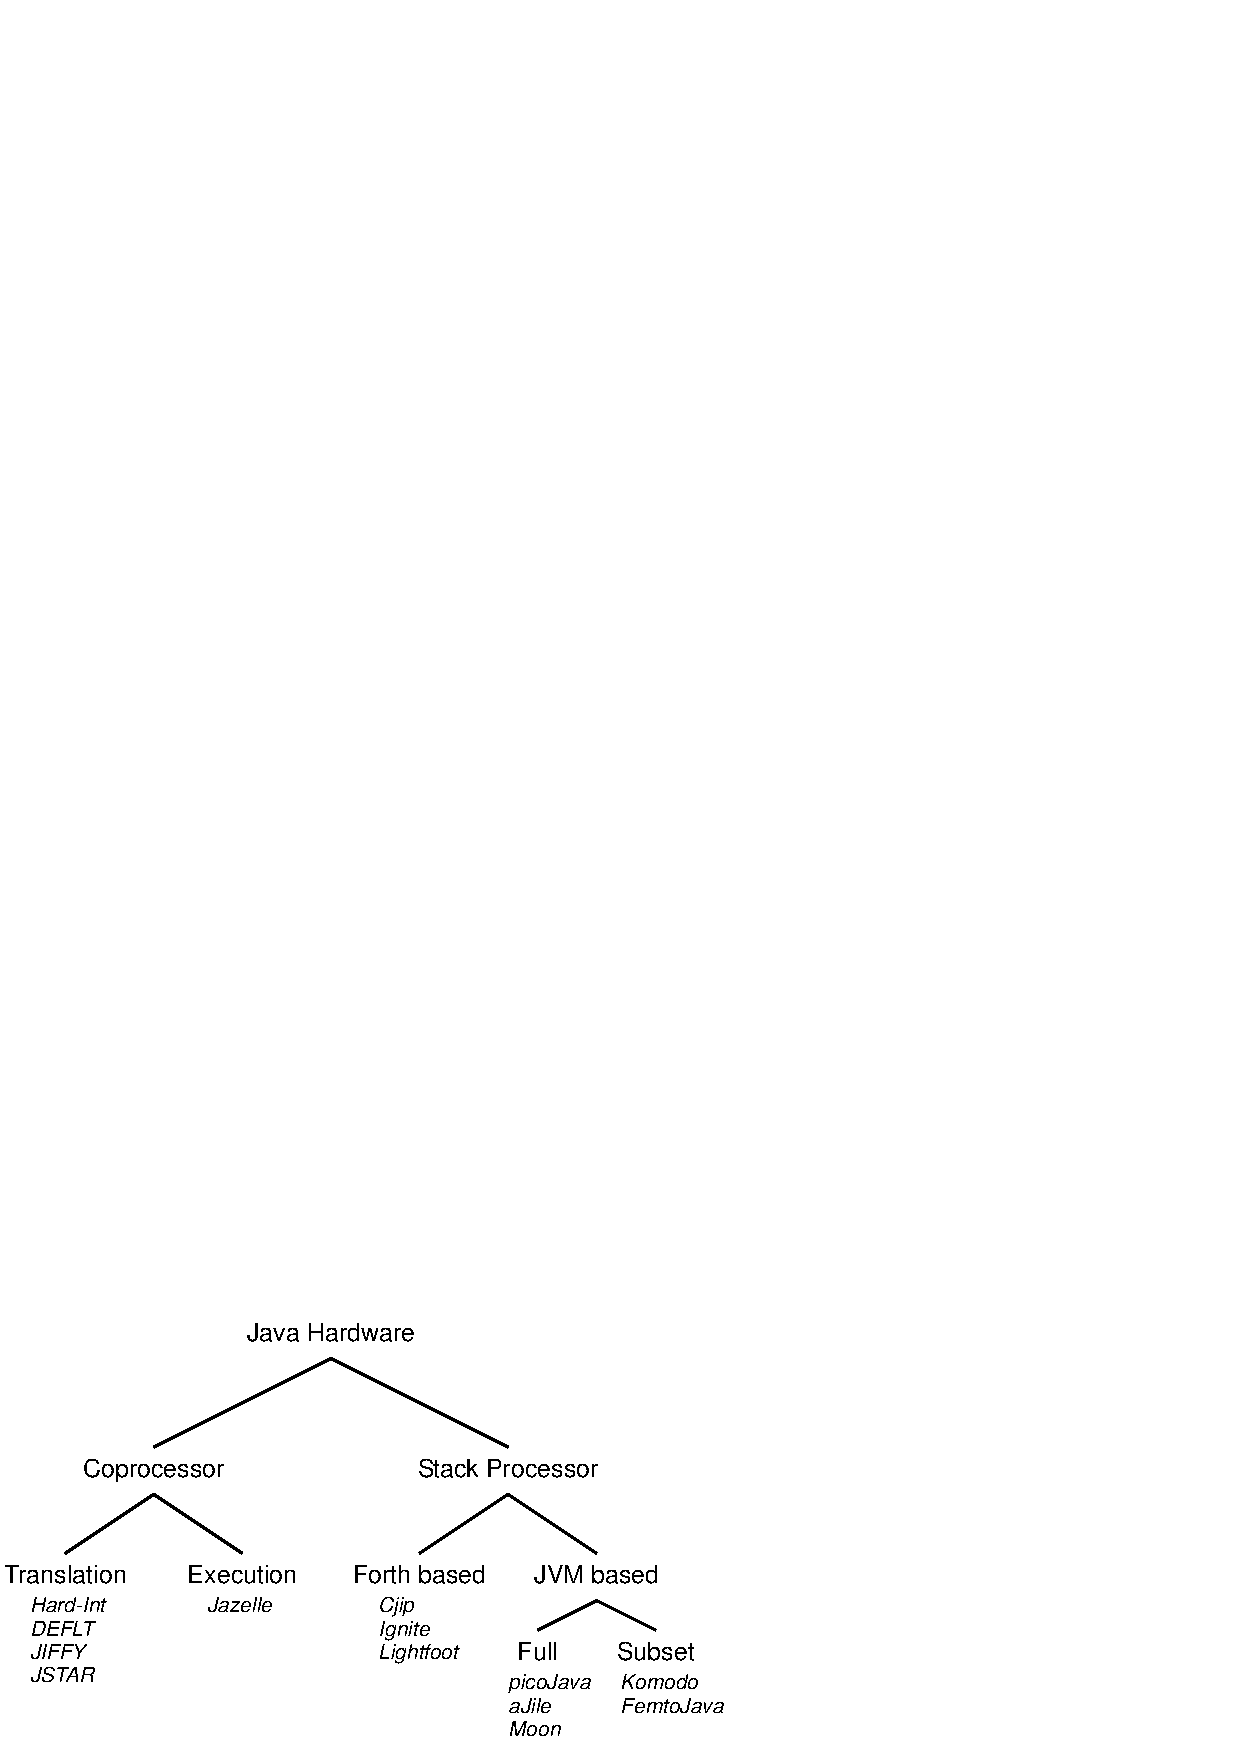
\includegraphics[scale=\picscale]{related/related_tree}
    \caption{Java hardware}
    \label{fig_related_tree}
\end{figure*}


There are problems in getting information about commercial products.
When new companies started developing Java processors, a lot of
information was available. This information was usually more of a
presentation of the concept, nevertheless it gave some insights into
how they approached the different design problems. However, at the
point at which the projects reached production quality, this
information quietly disappeared from their websites. It was replaced
with colorful marketing prospectuses about the wonderful world of
the new Java-enabled mobile phones. Only one company, aJile Ltd.,
presented information about their product in a refereed conference
paper.

Many research projects for a Java processor in an FPGA exists.
Examples can be found in \cite{Femto01}, \cite{Kim2000} and
\cite{368445}. These projects have much in common -- the basic
implementation of a stack machine with integer instructions is easy.
However, the realization of the complete JVM is the hard part and
therefore beyond the scope of these projects.

Other than the aJile processor and the Komodo project, no solution
addresses the problem of real-time predictability. For this reason,
as well as its availability, the aJile processor is used for
comparison with JOP.

\section{Summary}
\label{sec:related:summary}

In Table~\ref{tab:related:plus:minus}, features of selected Java
processors are compared. Category `Predictability' means how well
the processor is time-predictable. In category `Size', the chip size
is estimated and category `Performance' means average performance.
The category `JVM conformance' lists how complete the implementation
of the JVM specification \cite{jvm} is. The `Flexibility' parameter
indicates how well the processor can be adapted to different
application domains.

The assessment of the various parameters is, however, somewhat
subjective as the information is mainly derived from written
documentation. In Section~\ref{sec:performance}, the overall
performance of various Java systems, including the aJile processor,
is compared with JOP.

The last column of the table shows the features required for JOP.
This is, therefore, our research objective in a nutshell.

\begin{table}[htp]
    \centering
    \begin{tabular}{lccccc}
        \toprule
                        & picoJava & aJile   & Komodo  & FemtoJava & JOP     \\
        \midrule
        Predictability  & $--$     & $\cdot$ & $-$     & $\cdot$   & $++$    \\
        Size            & $--$     & $-$     & $+$     & $-$       & $++$    \\
        Performance     & $++$     & $+$     & $-$     & $--$      & $+$     \\
        JVM conformance & $++$     & $+$     & $-$     & $--$      & $\cdot$ \\
        Flexibility     & $--$     & $--$    & $+$     & $++$      & $++$    \\
        \bottomrule
    \end{tabular}
    \caption{Feature comparison of selected Java processors}
    \label{tab:related:plus:minus}
\end{table}

Due to the great variation in execution times for a trap, picoJava
is given a double minus in the `Predictability' category. picoJava
is also the largest processor in the list. However, its performance
and JVM compatibility are expected to be superior to those of other
processors.

The aJile processor is intended as a solution for real-time systems.
However, no information is available about bytecode execution times.
As this processor is a commercial product and has been on the market
for some time, it is expected that its JVM implementation would
conform to Java standards, as defined by Sun.

Komodos multithreading is similar to hyper-threading in modern
processors that are trying to hide latencies in instruction
fetching. However, this feature leads to very pessimistic WCET
values (in effect rendering the performance gain useless). The fact
that the pipeline clock is only a quarter of the system clock also
wastes a considerable amount of potential performance.

FemtoJava is given a double plus for flexibility, due to the
application-dependent generation of the processor. However,
FemtoJava is only a 16-bit processor and therefore not JVM
compliant. The resource usage is also very high, compared to the
minimal Java subset implemented and the low performance of the
processor.

So far, all processors in the list perform weakly in the area of
time-predictable execution of Java bytecodes. However, a low-level
analysis of execution times is of primary importance for WCET
analysis. Therefore, the main objective of JOP is to define and
implement a processor architecture that is as predictable as
possible. However, it is equally important that this does not result
in a low performance solution. Performance shall not suffer as a
result of the time-predictable architecture.

The second main aim of this work is to design a small processor.
Size and the resulting energy consumption are a main concern in
embedded systems. The proposed Java processor needs to be small
enough to be implemented in a low-cost FPGA device. With this
constraint, an implementation in an ASIC will also result in a very
small core that can be part of a larger system-on-a-chip.

The embedded market is diverse and one size does not fit all. A
configurable processor in which we can trade size for performance
provides the flexibility for a variety of application domains. The
aim of the architecture of JOP is to support this flexibility.

%\section{Derived Work}
%\label{sec:derived}
%
%Quite common for open-source projects are derived projects.
%Especially the research community appreciates open-source projects.
%Following list describes projects that are either completely based
%on JOP or influenced to a great extent.
%
%JOP triggered research on implementation of the JVM in hardware for
%real-time systems. The publications on JOP and also the fact that
%JOP is open-source made the project and ideas easy accessible for
%other researchers. Several research projects are directly or
%indirectly based on the research project JOP:
%
%\begin{itemize}
%    \item Lund -- Flavius
%    \item Dresden
%    \item Graz
%    \item Albertos MS thesis
%    \item \cite{conf/iscas/KoT07} JOP based dual-issue Javaprocessor
%    \item WCET work by Rasmus, Trevor, Elena, and upcoming CISS
%\end{itemize}



\chapter{Summary}
\label{chap:conclusions}

    
In this chapter we will undertake a short review of the project and
summarize the contributions. Java for real-time systems is a very
new and active research area. This chapter is completed by
suggestions for future research, based on the proposed Java
processor.

\section{Conclusions}

In the following list, we draw conclusions about the Java processor
presented in this document, in relation to the problem stated in
Section~\ref{sec:resques}:
\begin{enumerate}
    \item
A time-predictable Java platform has been demonstrated. As shown in
Section~\ref{sec:rtpredict} and \ref{sec:cache}, the architectural
design decisions and a time-predictable cache provide the basis for
a time-predictable Java processor. In Section~\ref{sec:wcet}, it was
shown that all bytecodes have a known WCET and there are no pipeline
dependencies. JOP's architecture can therefore be modeled
cycle-accurately for the low-level WCET analysis.
    \item
The implementation of a RISC-style stack architecture, with a novel
mapping of Java bytecodes to microcode addresses (see
Section~\ref{sec:microcode}), and the analysis of the JVM stack
usage pattern (see Section~\ref{sec:stack}) with the
resource-efficient two-level stack cache resulted in a small design.
In fact, JOP is the smallest implementation of the JVM in hardware
available to date.
    \item
The usage of JOP in real-world applications, as described in
Section~\ref{sec:applications}, shows that JOP is a working
processor and not only a theoretical architecture.
    \item
Comparing JOP with various embedded Java solutions in
Section~\ref{sec:performance} showed that the time-predictable
processor architecture does not need to be slow. JOP's average
performance is similar to that of non real-time Java systems.
    \item
The flexibility of an FPGA allows for a HW/SW-co-design approach,
with the aim of generating application-specific configurations of
JOP.
    \item
In Section~\ref{sec:rtprof}, a simple real-time profile for Java was
defined. This profile solves a number of issues that arise from
using standard Java for real-time systems. This profile was
elaborated upon in Section~\ref{sec:usersched} to create a framework
for a user-defined scheduler in Java, thus enabling the
implementation of advanced scheduling concepts at the application
level.
\end{enumerate}

\section{Summary of Contributions}

The research contributions made by this work are related to two
areas: real-time Java and resource-constrained embedded systems.

\subsubsection{A Real-Time Java Processor}

The goal of time-predictable execution of Java programs was a
first-class guiding principle throughout the development of JOP:

\begin{itemize}

        \item
The execution time for Java bytecodes can be exactly predicted in
terms of the number of clock cycles.
% The execution time for Java bytecodes is known cycle-accurate.
JOP is therefore a straightforward target for low-level WCET
analysis. There is no mutual dependency between consecutive
bytecodes that could result in unbounded timing effects.

    \item
In order to provide time-predictable execution of Java bytecodes,
the processor pipeline is designed without any prefetching or
queuing. This fact avoids hard-to-analyze and possibly unbounded
pipeline dependencies. There are no pipeline stalls, caused by
interrupts or the memory subsystem, to complicate the WCET analysis.

    \item
A pipelined processor architecture calls for higher memory
bandwidth. A standard technique to avoid processing bottlenecks due
to the higher memory bandwidth is caching.
%In order to fill the gap between processor speed and the memory
%access time, caches are mandatory, even in embedded systems.
However, standard cache organizations improve the average execution
time but are difficult to predict for WCET analysis. Two
time-predictable caches are proposed for JOP: a \emph{stack cache}
as a substitution for the data cache and a \emph{method cache} to
cache the instructions.

As the stack is a heavily accessed memory region, the stack -- or
part of it -- is placed in local memory. This part of the stack is
referred to as the \emph{stack cache} and described in
Section~\ref{sec:stack}. Fill and spill of the stack cache is
subjected to microcode control and therefore time-predictable.

In Section~\ref{sec:cache}, a novel way to organize an instruction
cache, as \emph{method cache}, is given. The cache stores complete
methods, and cache misses only occur on method invocation and
return. Cache block replacement depends on the call tree, instead of
instruction addresses. This \emph{method cache} is easy to analyze
with respect to worst-case behavior and still provides substantial
performance gain when compared against a solution without an
instruction cache.

    \item
The above described time-predictable processor provides the basis
for real-time Java. The issues with standard Java and the Real-Time
Specification for Java were analyzed in Chapter~\ref{chap:rtjava}.
To enable real-time Java to operate on resource-constrained devices,
a simple real-time profile was defined in Section~\ref{sec:rtprof}
and implemented in Java on JOP. The beauty of this approach is in
implementing functions usually associated with an RTOS in Java. This
means that real-time Java is not based on an RTOS, and therefore not
restricted to the functionality provided by the RTOS. With JOP, a
self-contained real-time system in pure Java becomes possible.

The tight integration of the scheduler and the hardware that
generates schedule events results in low latency and low jitter of
the task dispatch.

    \item
%The timer interrupt in JOP generates interrupts at the release times
%of the tasks. The scheduler is responsible for reprogramming the
%timer after each occurrence of a timer interrupt. Controlling the
%timer interrupt as part of the scheduling results in the low jitter
%of periodic tasks.
%
The defined real-time profile suggests a new way to handle hardware
interrupts to avoid interference between blocking device drivers and
application tasks. Hardware interrupts other than the timer
interrupt are represented as asynchronous events with an associated
thread. These events are \emph{normal} schedulable objects and
subject to the control of the scheduler. With a minimum interarrival
time, these events, and the associated device drivers, can be
incorporated into the priority assignment and schedulability
analysis in the same way as normal application tasks.

\end{itemize}

The above-described contributions result in a time-predictable
execution environment for real-time applications written in Java,
without the resource implications and unpredictability of a
JIT-compiler. The proposed processor architecture is a
straightforward target for low-level WCET analysis.

%New applications, such as multimedia streaming, result in
%\emph{soft} real-time systems that need a more flexible scheduler
%than the traditional fixed priority-based ones.

Implementing a real-time scheduler in Java opens up new
possibilities. The scheduler is extended to provide a framework for
user-defined scheduling in Java. In Section~\ref{sec:usersched}, we
analyzed which events are exposed to the scheduler and which
functions from the JVM need to be available in the user space. A
simple-to-use framework to evaluate new scheduling concepts is
given.



\subsubsection{A Resource-Constrained Processor}

Embedded systems are usually very resource-constrained. Using a
low-cost FPGA as the main target technology forced the design to be
small. The following architectural features address this issue:

\begin{itemize}

    \item
The architecture of JOP is best described as:
\begin{quote}
    The JVM is a CISC stack architecture, whereas JOP is a RISC stack
    architecture.
\end{quote}
JOP contains its own instruction set, called microcode in this
thesis, with a novel way of mapping bytecodes to microcode
addresses. This mapping has zero overheads as described in
Section~\ref{sec:microcode}. Basic bytecode instructions have a
one-to-one mapping to microcode instructions and therefore execute
in a single cycle. The stack architecture allows compact encoding of
microinstructions in 8 bit to save internal memory.

This approach allows flexible implementation of Java bytecodes in
hardware, as a microcode sequence or even in Java itself.

    \item
The analysis of the JVM stack usage pattern in
Section~\ref{sec:stack} led to the design of a resource-efficient
two-level stack cache. This two-level stack cache fits to the
embedded memory technologies of current FPGAs and ASICs and ensures
fast execution of basic instructions.

Part of the stack cache, which is implemented in an on-chip memory,
is also used for microcode variables and constants. This resource
sharing does not only reduce the number of memory blocks needed for
the processor, but also the number of data paths to and from the
execution unit.

    \item
Interrupts are considered hard to handle in a pipelined processor,
resulting in a complex (and therefore resource consuming)
implementation. In JOP, the above mentioned bytecode-microcode
mapping is used in a clever way to avoid interrupt handling in the
core pipeline.
%
%An implementation of interrupts at the bytecode-microcode mapping
%keeps interrupts transparent in the core pipeline and avoids complex
%logic. Therefore,
%
Interrupts generate special bytecodes that are inserted in a
transparent way in the bytecode stream. Interrupt handlers can be
implemented in the same way as bytecodes are implemented: in
microcode or in Java.


\end{itemize}

The above design decisions where chosen to keep the size of the
processor small without sacrificing performance. JOP is the smallest
Java processor available to date that provides the basis for an
implementation of the CLDC specification (see
Section~\ref{subsec:cldc}). JOP is a fast execution environment for
Java, without the resource implications and unpredictability of a
JIT-compiler. The average performance of JOP is similar to that of
mainstream, non real-time Java systems.

JOP is a flexible architecture that allows different configurations
for different application domains. Therefore, size can be traded
against performance. As an example, resource intensive instructions,
such as floating point operations, can be implemented in Java. The
flexibility of an FPGA implementation also allows adding
application-specific hardware accelerators to JOP.

The small size of the processor allows usage of low-cost FPGAs in
embedded systems that can compete against standard microcontroller.
JOP has been implemented in several different FPGA families and is
used in different real-world applications.

Programs for embedded and real-time systems are usually
multi-threaded and a small design provides a path to a
multi-processor system in a mid-sized FPGA or in an ASIC.

A tiny architecture also opens new application fields when
implemented in an ASIC. Smart sensors and actuators, for example,
are very sensitive to cost, which is proportional to the die area.


\section{Future Research Directions}

JOP provides a basis for various directions for future research.
Some suggestions are given below:
%
\begin{description}
    \item[Real-time garbage collector:]
In Section~\ref{sec:gc}, a real-time garbage collector was
presented. Hardware support of a real-time GC would be an
interesting topic for further research.

Another question that remains with a real-time GC is the analysis of
the worst-case memory consumptions of tasks (similar to the WCET
values), and scheduling the GC so that it can keep up with the
allocation rate.

    \item[Hardware accelerator:]
The flexibility of an FPGA implementation of a processor opens up
new possibilities for hardware accelerators. We have shown in
Section~\ref{sec:hwsw:co} how the implementation of a bytecode can
be moved between hardware and software. A further step would be to
generate an application specific-system in which part of the
application code is moved to hardware. Ideally, the hardware
description should be extracted automatically from the Java source.
Preliminary work in this area, using JOP as its basis, can be found
in \cite{jop:sac05}.

    \item[Hardware scheduler:]
In JOP, scheduling and dispatch is done in Java (with some microcode
support). For tasks with very short periods, the scheduling
overheads can prove to be too high. A scheduler implemented in
hardware can shorten this time, due to the parallel nature of the
algorithm.

    \item[Multiprocessor JVM:]
In order to generate a small and predictable processor, several
advanced and resource-consuming features (such as instruction
folding or branch prediction) were omitted from the design. The
resulting low resource usage of JOP makes it possible to integrate
more than one processor in an FPGA. Since embedded applications are
naturally multi-threaded systems, the performance can easily be
enhanced using a multi-processor solution. A multi-processor JVM
with shared memory offers following research possibilities:
scheduling of Java threads and synchronization between the
processors; WCET analysis for the shared memory access.

First results on a JOP CMP are described in \cite{jop:dma, jop:cmp}.

    \item[Instruction cache:]
The cache solution proposed in Section~\ref{sec:cache} provides
predictable instruction cache behavior while, in the average case,
still performing in a similar way to a direct-mapped cache. However,
an analysis tool for the worst-case behavior is still needed. With
this tool, and a more complex analysis tool for traditional
instruction caches, we also need to verify that the worst-case miss
penalty is lower than with a traditional instruction cache.

A second interesting aspect of the proposed method cache is the fact
that the replacement decision on a cache miss only occurs on method
invoke and return. The infrequency of this decision means that more
time is available for more advanced replacement algorithms.


    \item[Real-time Java:]
Although there is already a definition for real-time Java, i.e.\ the
RTSJ \cite{rtsj}, this definition is not necessarily adequate. There
is ongoing research on how memory should be managed for real-time
Java applications: scoped memory, as suggested by the RTSJ, usage of
a real-time GC, or application managed memory through memory pools.
However, almost no research has been done into how the Java library
which has proven a major part of Java's success, can be used in
real-time systems or how it can be adapted to do so. The question of
what the best memory management is for the Java standard library
remains unanswered.

    \item[Java computer:]
How would a processor architecture and operating system architecture
look in a `Java only' system? Here, we need to rethink our approach
to processes, protection, kernel- and user-space, and virtual
memory. The standard approach of using memory protection between
different processes is necessary for applications that are
programmed in languages that use memory addresses as data, i.e.\
pointer usage and pointer manipulation. In Java, no memory addresses
are visible and pointer manipulation is not possible. This very
important feature of Java makes Java a \emph{safe} language.
Therefore, an error-free JVM means we do not need memory protection
between processes and we do not need to make a distinction between
kernel and user space (with all the overhead) in a Java system.
Another reason for using virtual addresses is link addresses.
However, in Java this issue does not exist, as all classes are
linked dynamically and the code itself (i.e.\ the bytecodes) only
uses relative addressing.

Another issue here is the paging mechanism in virtual memory system,
which has to be redesigned for a Java computer. For this, we need to
merge the virtual memory management with the GC. It does not make
sense to have a virtual memory manager that works with plain (e.g.\
4KB) memory pages without knowledge about object lifetime. We
therefore need to incorporate the virtual memory paging with a
generational GC. The GC knows which objects have not been accessed
for a long time and can be swapped out to the disc. Handling paging
as part of the GC process also avoids page fault exceptions and
thereby simplifies the processor architecture.

Another question is whether we can substitute the process notation
with threads, or whether we need several JVMs on a Java only system.
It depends. If we can live with the concept of shared static class
members, we can substitute heavyweight processes with lightweight
threads. It is also possible that we would have to define some
further thread local data structures in the operation system.

\end{description}
%
It is the opinion of the author that Java is a promising language
for future real-time systems. However, a number of issues remain to
be solved. JOP, with its time-predictable execution of Java
bytecodes, is an important but nevertheless only a small part of a
real-time Java system.



%\pagestyle{empty}
%\chaptermark{} % remove chapter mark in the heading, but it does it on the
               % last page too!



%\def\rightmark{} % remove section part in the heading
\appendix
 \ihead{\leftmark} % use chapter (=\leftmark) on both pages in the appendix

\chapter{Publications}
    % This is a copy from /usr/doc

\begin{itemize}

\subsubsection*{2003}

\item Martin Schoeberl.
 Using a {J}ava Optimized Processor in a Real World Application.
 In {\em Proceedings of the First Workshop on Intelligent Solutions in
  Embedded Systems (WISES 2003)}, pages 165--176, Austria, Vienna, June 2003.

\item Martin Schoeberl.
 Design Decisions for a {J}ava Processor.
 In {\em Tagungsband Austrochip 2003}, pages 115--118, Linz, Austria,
  October 2003.

\item Martin Schoeberl.
 {JOP}: {A} {J}ava Optimized Processor.
 In R.~Meersman, Z.~Tari, and D.~Schmidt, editors, {\em On the Move to
  Meaningful Internet Systems 2003: Workshop on {J}ava Technologies for
  Real-Time and Embedded Systems (JTRES 2003)}, volume 2889 of {\em Lecture
  Notes in Computer Science}, pages 346--359, Catania, Italy, November 2003.
  Springer.

\subsubsection*{2004}

\item Martin Schoeberl.
 Restrictions of {J}ava for Embedded Real-Time Systems.
 In {\em Proceedings of the 7th IEEE International Symposium on
  Object-Oriented Real-Time Distributed Computing (ISORC 2004)}, pages
  93--100, Vienna, Austria, May 2004.

\item Martin Schoeberl.
 Design Rationale of a Processor Architecture for Predictable
  Real-Time Execution of {J}ava Programs.
 In {\em Proceedings of the 10th International Conference on
  Real-Time and Embedded Computing Systems and Applications (RTCSA 2004)},
  Gothenburg, Sweden, August 2004.

\item Martin Schoeberl.
 Real-Time Scheduling on a {J}ava Processor.
 In {\em Proceedings of the 10th International Conference on
  Real-Time and Embedded Computing Systems and Applications (RTCSA 2004)},
  Gothenburg, Sweden, August 2004.

\item Martin Schoeberl.
 {J}ava Technology in an {FPGA}.
 In {\em Proceedings of the International Conference on
  Field-Programmable Logic and its applications (FPL 2004)}, Antwerp, Belgium,
  August 2004.

\item Martin Schoeberl.
 A Time Predictable Instruction Cache for a Java Processor.
 In Robert Meersman, Zahir Tari, and Angelo Corsario, editors, {\em On
  the Move to Meaningful Internet Systems 2004: Workshop on {J}ava Technologies
  for Real-Time and Embedded Systems (JTRES 2004)}, volume 3292 of {\em
  Lecture Notes in Computer Science}, pages 371--382, Agia Napa, Cyprus,
  October 2004. Springer.

\subsubsection*{2005}

\item Flavius Gruian, Per Andersson, Krzysztof Kuchcinski, and Martin Schoeberl.
 Automatic generation of application-specific systems based on a
  micro-programmed java core.
 In {\em Proceedings of the 20th ACM Symposium on Applied Computing,
  Embedded Systems track}, Santa Fee, New Mexico, March 2005.

\item Martin Schoeberl.
 Design and implementation of an efficient stack machine.
 In {\em Proceedings of the 12th IEEE Reconfigurable Architecture
  Workshop (RAW2005)}, Denver, Colorado, USA, April 2005. IEEE.

\item Martin Schoeberl.
 {\em JOP: A Java Optimized Processor for Embedded Real-Time Systems}.
 PhD thesis, Vienna University of Technology, 2005.

\item Martin Schoeberl.
 Evaluation of a {J}ava processor.
 In {\em Tagungsband Austrochip 2005}, pages 127--134, Vienna,
  Austria, October 2005.

\subsubsection*{2006}

\item Martin Schoeberl.
 A time predictable {J}ava processor.
 In {\em Proceedings of the Design, Automation and Test in Europe
  Conference (DATE 2006)}, pages 800--805, Munich, Germany, March 2006.

\item Martin Schoeberl.
 Real-time garbage collection for {J}ava.
 In {\em Proceedings of the 9th IEEE International Symposium on Object
  and Component-Oriented Real-Time Distributed Computing (ISORC 2006)}, pages
  424--432, Gyeongju, Korea, April 2006.

\item Martin Schoeberl. Instruction Cache f\"ur Echtzeitsysteme,
    April 2006. Austrian patent AT 500.858.

\item Rasmus Pedersen and Martin Schoeberl.
 An embedded support vector machine.
 In {\em Proceedings of the Fourth Workshop on Intelligent Solutions
  in Embedded Systems (WISES 2006)}, pages 79--89, Jun. 2006.

\item Rasmus Pedersen and Martin Schoeberl.
 Exact roots for a real-time garbage collector.
 In {\em Proceedings of the Workshop on {J}ava Technologies for
  Real-Time and Embedded Systems (JTRES 2006)}, Paris, France, October 2006.

\item Martin Schoeberl and Rasmus Pedersen.
 {WCET} analysis for a {Java} processor.
 In {\em Proceedings of the Workshop on {J}ava Technologies for
  Real-Time and Embedded Systems (JTRES 2006)}, Paris, France, October 2006.

\subsubsection*{2007}

\item Martin Schoeberl, Hans Sondergaard, Bent Thomsen, and Anders~P. Ravn.
A profile for safety critical java.
In {\em 10th IEEE International Symposium on Object and
  Component-Oriented Real-Time Distributed Computing (ISORC'07)}, pages
  94--101, Santorini Island, Greece, May 2007. IEEE Computer Society.

\item Martin Schoeberl.
Mission modes for safety critical java.
In {\em 5th IFIP Workshop on Software Technologies for Future
  Embedded \& Ubiquitous Systems}, May 2007.

\item Raimund Kirner and Martin Schoeberl.
Modeling the function cache for worst-case execution time analysis.
In {\em Proceedings of the 44rd Design Automation Conference, DAC
  2007}, San Diego, CA, USA, June 2007. ACM.

\item Martin Schoeberl.
A time-triggered network-on-chip.
In {\em International Conference on Field-Programmable Logic and its
  Applications (FPL 2007)}, Amsterdam, Netherlands, August 2007.

\item Christof Pitter and Martin Schoeberl.
Time predictable {CPU} and {DMA} shared memory access.
In {\em International Conference on Field-Programmable Logic and its
  Applications (FPL 2007)}, Amsterdam, Netherlands, August 2007.


\item Wolfgang Puffitsch and Martin Schoeberl.
{picoJava-II} in an {FPGA}.
In {\em Proceedings of the 5th international workshop on Java
  technologies for real-time and embedded systems (JTRES 2007)}, Vienna,
  Austria, September 2007. ACM Press.

\item Martin Schoeberl.
Architecture for object oriented programming languages.
In {\em Proceedings of the 5th international workshop on Java
  technologies for real-time and embedded systems (JTRES 2007)}, Vienna,
  Austria, September 2007. ACM Press.

\item Christof Pitter and Martin Schoeberl.
Towards a {Java} multiprocessor.
In {\em Proceedings of the 5th international workshop on Java
  technologies for real-time and embedded systems (JTRES 2007)}, Vienna,
  Austria, September 2007. ACM Press.

\item Martin Schoeberl and Jan Vitek.
Garbage collection for safety critical {Java}.
In {\em Proceedings of the 5th international workshop on Java
  technologies for real-time and embedded systems (JTRES 2007)}, Vienna,
  Austria, September 2007. ACM Press.

\item Martin Schoeberl. {SimpCon} - a simple and efficient {SoC}
    interconnect. In {\em Proceedings of the 15th Austrian
    Workhop on Microelectronics, Austrochip 2007}, Graz, Austria,
  October 2007.

\subsubsection*{2008}

\item Martin Schoeberl. A Java processor architecture for
    embedded real-time systems. {\em Journal of Systems
    Architecture}, 54/1--2:265--286, 2008.

\item Trevor Harmon, Martin Schoeberl, Raimund Kirner, and
    Raymond Klefstad. A modular worst-case execution time
    analysis tool for Java
  processors. In {\em Proceedings of the 14th IEEE Real-Time and
 Embedded Technology and Applications Symposium (RTAS 2008)}, St.
 Louis, MO, United States, April 2008.

\item Martin Schoeberl, Stephan Korsholm, Christian Thalinger,
    and Anders~P. Ravn. Hardware objects for {Java}. In {\em
    Proceedings of the 11th IEEE International Symposium on
  Object/component/service-oriented Real-time distributed
  Computing (ISORC 2008)}, Orlando, Florida, USA, May 2008. IEEE
  Computer Society.

\item Stephan Korsholm, Martin Schoeberl, and Anders~P. Ravn.
    Interrupt Handlers in {Java}.
 In {\em Proceedings of the 11th IEEE International Symposium on
  Object/component/service-oriented Real-time distributed
  Computing (ISORC 2008)}, Orlando, Florida, USA, May 2008. IEEE
  Computer Society.

\item Trevor Harmon, Martin Schoeberl, Raimund Kirner, and
    Raymond Klefstad. Toward libraries for real-time Java. In
    {\em Proceedings of the 11th IEEE International Symposium on
    Object/component/service-oriented Real-time distributed
  Computing (ISORC 2008)}, Orlando, Florida, USA, May 2008. IEEE
  Computer Society.

\item Christof Pitter and Martin Schoeberl. Performance
    evaluation of a {Java} chip-multiprocessor. In {\em
    Proceedings of the 3rd IEEE Symposium on Industrial Embedded
    Systems (SIES 2008)}, Jun. 2008.

\item Martin Schoeberl. Application experiences with a real-time
    {J}ava processor. In {\em Proceedings of the 17th IFAC World
    Congress}, Seoul, Korea, July 2008.

\item Peter Puschner and Martin Schoeberl. On composable system
    timing, task timing, and WCET analysis. In {\em Proceedings
    of the 8th International Workshop on Worst-Case Execution
    Time (WCET) Analysis}, Prague, Czech
  Republic, July 2008.

\item Martin Schoeberl. {\em JOP: A Java Optimized Processor for
    Embedded Real-Time Systems}. Number ISBN 978-3-8364-8086-4.
    VDM Verlag Dr. M{\"u}ller, July 2008.

\item Martin Schoeberl and Wolfgang Puffitsch. Non-blocking
    object copy for real-time garbage collection. In {\em
    Proceedings of the 6th International Workshop on Java
  Technologies for Real-time and Embedded Systems (JTRES 2008)},
  September 2008.

\item Wolfgang Puffitsch and Martin Schoeberl. Non-blocking root
    scanning for real-time garbage collection. In {\em
    Proceedings of the 6th International Workshop on Java
  Technologies for Real-time and Embedded Systems (JTRES 2008)},
  September 2008.

\item Walter Binder, Martin Schoeberl, Philippe Moret, and Alex
    Villazon. Cross-profiling for embedded Java processors. In
    {\em Proceedings of the 5th International Conference on the
    Quantitative Evaluation of SysTems (QEST 2008)}, St Malo,
  France, September 2008.

\item Walter Binder, Alex Villazon, Martin Schoeberl, and
    Philippe Moret. Cache-aware cross-profiling for Java
    processors. In {\em Proceedings of the 2008 international
    conference on Compilers, architecture, and synthesis
    forembedded systems (CASES 2008)}, Atlanta, Georgia, October
    2008. ACM.

\subsubsection*{2009}

\item Martin Schoeberl. Time-predictable computer architecture.
    {\em EURASIP Journal on Embedded Systems}, vol. 2009, Article
    ID 758480:17 pages, 2009.

\item Martin Schoeberl. Time-predictable cache organization. In
    {\em Proceedings of the First International Workshop on
    Software Technologies for Future Dependable Distributed
    Systems (STFSSD 2009)}, Tokyo, Japan, March
  2009. IEEE Computer Society.

\item Andy Wellings and Martin Schoeberl. Thread-local scope
    caching for real-time {J}ava. In {\em Proceedings of the 12th
    IEEE International Symposium on
  Object/component/service-oriented Real-time distributed
  Computing (ISORC 2009)}, Tokyo, Japan, March 2009. IEEE
  Computer Society.

\item Florian Brandner, Tommy Thorn, and Martin Schoeberl.
    Embedded {JIT} compilation with {CACAO} on {YARI}. In {\em
    Proceedings of the 12th IEEE International Symposium on
    Object/component/service-oriented Real-time
  distributed Computing (ISORC 2009)}, Tokyo, Japan, March 2009.
  IEEE Computer Society.

\item Thomas Henties, James~J. Hunt, Doug Locke, Kelvin Nilsen,
    Martin Schoeberl, and Jan Vitek. Java for safety-critical
 applications. In {\em 2nd International Workshop on the
 Certification of Safety-Critical Software Controlled Systems
 (SafeCert 2009)}, Mar. 2009.

\item Martin Schoeberl and Peter Puschner. Is
    chip-multiprocessing the end of real-time scheduling? In {\em
    Proceedings of the 9th International Workshop on Worst-Case
  Execution Time (WCET) Analysis}, Dublin, Ireland, July 2009.
  OCG.

\item Benedikt Huber and Martin Schoeberl. Comparison of implicit
    path enumeration and model checking based WCET
  analysis. In {\em Proceedings of the 9th International Workshop
on Worst-Case
  Execution Time (WCET) Analysis}, Dublin, Ireland, July 2009.
  OCG.

\item Philippe Moret, Walter Binder, Martin Schoeberl, Alex
    Villazon, and Danilo Ansaloni. Analyzing performance and
dynamic behavior of embedded Java software with calling-context
  cross-profiling. In {\em Proceedings of
the 7th International Conference on the Principles and Practice
  of Programming in Java (PPPJ 2009)}, Calgary, Alberta, Canada,
  August 2009. ACM.

\item Martin Schoeberl, Walter Binder, Philippe Moret, and Alex
    Villazon. Design space exploration
for Java processors with cross-profiling. In {\em Proceedings of
the 6th International Conference on the Quantitative Evaluation
  of SysTems (QEST 2009)}, Budapest, Hungary, September 2009.
  IEEE Computer Society.

\item Philippe Moret, Walter Binder, Alex Villazon, Danilo
    Ansaloni, and Martin Schoeberl. Locating performance
    bottlenecks in embedded Java software with
  calling-context cross-profiling. In {\em Proceedings of the 6th
International Conference on the
  Quantitative Evaluation of SysTems (QEST 2009)}, Budapest,
  Hungary, September 2009. IEEE Computer Society.

\item Jack Whitham, Neil Audsley, and Martin Schoeberl. Using
    hardware methods to improve time-predictable performance in
  real-time java systems. In {\em Proceedings of the 7th
International Workshop on Java
  Technologies for Real-time and Embedded Systems (JTRES 2009)},
  Madrid, Spain, September 2009. ACM Press.


\subsubsection*{2010}

\item Martin Schoeberl and Wolfgang Puffitsch. Non-blocking
    real-time garbage collection. {\em Trans. on Embedded
    Computing Sys.}, accepted, 2010.

\item Christof Pitter and Martin Schoeberl. A real-time {Java}
    chip-multiprocessor. {\em Trans. on Embedded Computing Sys.},
    accepted, 2010.

\item Walter Binder, Martin Schoeberl, Philippe Moret, and Alex
    Villazon. Cross-profiling for Java processors. {\em Software:
Practice and Experience}, accepted, 2010.

\end{itemize}


%\chapter{Glossary}
\chapter{Acronyms}
 \label{appx:acro}
\newcommand{\gloss}[3]{
    \textbf{#1} & #2\\
%    \item[#1] {#2}\\{#3}
%    \textbf{#1} & #2\\ & \mbox{#3}\\
%    \textbf{#1} \> \> #2\\ \> \parbox{10cm}{#3}\\ \\
}
\begin{longtable}[l]{ll}
%    abc\=WCET\= \kill % for tabbing
    \gloss{ADC}{Analog to Digital Converter}{}
    \gloss{ALU}{Arithmetic and Logic Unit}{The part of a processor that performs
    arithmetic, logical, and related operations.}
    \gloss{ASIC}{Application-Specific Integrated Circuit}{}
    \gloss{BCET}{Best Case Execution Time}{}
    \gloss{CFG}{Control Flow Graph}{}
    \gloss{CISC}{Complex Instruction Set Computer}{}
    \gloss{CLDC}{Connected Limited Device Configuration}{}
    \gloss{CPI}{average Clock cycles Per Instruction}{}
    \gloss{CRC}{Cyclic Redundancy Check}{}
    \gloss{DMA}{Direct Memory Access}{}
    \gloss{DRAM}{Dynamic Random Access Memory}{}
    \gloss{EDF}{Earliest Deadline First}{}
    \gloss{EMC}{Electromagnetic Compatibility}{}
    \gloss{ESD}{Electrostatic Discharge}{}
    \gloss{FIFO}{Fist In, First Out}{}
    \gloss{FPGA}{Field Programmable Gate Array}{FPGAs are a class of programmable
    logic devices. They contain a matrix of
    LCs, embedded memory blocks, and sophisticated I/O cells.}
    \gloss{GC}{Garbage Collect(ion/or)}{}
    \gloss{IC}{Instruction Count}{}
    \gloss{ILP}{Instruction Level Parallelism}{}
    \gloss{JOP}{Java Optimized Processor}{A processor that implements the JVM
    in hardware with architectural features for time-predictable execution of
    Java applications for real-time systems.}
    \gloss{J2ME}{Java2 Micro Edition}{}
    \gloss{J2SE}{Java2 Standard Edition}{}
    \gloss{JDK}{Java Development Kit}{}
    \gloss{JIT}{Just-In-Time}{}
    \gloss{JVM}{Java Virtual Machine}{}
    \gloss{LC}{Logic Cell}{The basic element in an FPGA: a 4-bit lookup table with
a register.}
    \gloss{LRU}{Least-Recently Used}{}
    \gloss{MBIB}{Memory Bytes read per Instruction Byte}{}
    \gloss{MCIB}{Memory Cycles per Instruction Byte}{}
    \gloss{MP}{Miss Penalty}{}
    \gloss{MTIB}{Memory Transactions per Instruction Byte}{}
    \gloss{MUX}{Multiplexer}{}
    \gloss{OO}{Object Oriented}{}
    \gloss{OS}{Operating System}{}
    \gloss{RISC}{Reduced Instruction Set Computer}{}
    \gloss{RT}{Real-Time}{}
    \gloss{RTOS}{Real-Time Operating System}{}
    \gloss{RTSJ}{Real-Time Specification for Java}{}
    \gloss{SCADA}{Supervisory Control And Data Acquisition}{}
    \gloss{SDRAM}{Synchronous DRAM}{}
    \gloss{SRAM}{Static Random Access Memory}{}
    \gloss{TOS}{Top Of Stack}{}
    \gloss{UART}{Universal Asynchronous Receiver/Transmitter}{}
    \gloss{VHDL}{Very High Speed Integrated Circuit (VHSIC)}{}
    \gloss{}{Hardware Description Language}{}
    \gloss{WCET}{Worst-Case Execution Time}{}
%    \gloss{xxx}{yyy}{}
%    \gloss{xxx}{yyy}{}
%    \gloss{xxx}{yyy}{}
\end{longtable}



\chapter{JOP Instruction Set} \label{appx:jop:instr}
%
% a changed copy from the thesis

%\documentclass[a4paper,10pt,twocolumn]{article}
% use option draft to check for typesetting problems.
% similar to original word document

% don't use textheight... with koma-script
\documentclass[%draft,
%    a4paper,12pt, % 'Standard'
    11pt, % use explicit paper format for Java book format
%    b5paper,10pt, % B5 printout
    % use BCOR to compensate for the two-side margin!
%    a4paper,12pt,BCOR37pt,DIV15,
%    a4paper,12pt,BCOR40pt,DIV14,
%    b5paper,10pt,DIV12,
    headinclude, footexclude,
    twoside, % this produces strange margins!
    openright, % for new chapters
    cleardoubleempty,
% normalheadings - smaller chapter or smallheadings - too small
    % abstracton, % the author of koma-script argues against the title
    headsepline,
%    5headlines, % standard is 1.25 -- wirkt net!
    pointlessnumbers,
    ]{scrreprt}

%\usepackage{html}

% headings
\usepackage{scrpage2} % for headers
 \setkomafont{pagehead}{\scshape\small}
 \setkomafont{pagenumber}{\scshape\small}
 \automark[section]{chapter}
 \ohead[]{\pagemark}
 \chead[]{}
 \ihead[]{\headmark}
 \ofoot[]{} \cfoot[]{} \ifoot[]{}

%\tolerance=500 % to avoid lines sticking out into the margin
               % needed for 'high-performance' in Intro - contributions
\emergencystretch=2em
% or tol. to 500 and emerg. to 1em?
% pagebreak was ok with 500 and 1em
\interfootnotelinepenalty=10000


% use BCOR = (paperwidth-textwidth)/4
% A4: 210mm x 297mm
% B5: 176mm x 250mm
% Java book: 185mm x 232mm
% Engblom: 120x188 (without head)
% Java: 127x187 (without head)
% 1pt = 1/72.27 in = 0.351 mm


% for book
% 'Java-format' 526pt x 660pt (Ghostscript)
\setlength{\paperwidth}{185mm} \setlength{\paperheight}{232mm}
% use that BCOR setting with twoside to compensate the margin
\areaset[13.75mm]{130mm}{200mm} % Java book format

% for book to A4 conversion:
% Set the following sizes and export with
% 'Variable Page Size' in gs.
% Print with 'fit to paper' in Acrobat - results in 110%
% and an effective text area of 142x215
%\setlength{\paperwidth}{180mm} \setlength{\paperheight}{232mm}
%\areaset[12.5mm]{130mm}{200mm} % Java book format

% for two page printout in .pdf
%\setlength{\paperwidth}{134mm} \setlength{\paperheight}{206mm}
%\areaset[1mm]{130mm}{200mm} % Java book format


% use 10pt for code instead of 11pt - but I still would prefer Lucida Typewriter
%\newfont{\myttfont}{cmss10 scaled 1000}
%\newfont{\myttbfont}{cmssdc10 scaled 1000}
%
% This IS Lucida Typewriter
%\newfont{\myttfont}{plsr8r scaled 950}
%\newfont{\myttbfont}{plsb8r scaled 950}
%\newfont{\myttifont}{plsro8r scaled 950}
%%\newfont{\mytttextfont}{plsr8r}

% Lucida is perhaps available in the new Tex installation!!!!
% does not really work!!!
\newfont{\myttfont}{hlsrt8r scaled 950}
\newfont{\myttbfont}{hlsbt8r scaled 950}
\newfont{\myttifont}{hlsrot8r scaled 950}

% I used these .ttf for the official Thesis
%..\ttf2pt1 -e -b LucidaTypewriterRegular.ttf plsr8a
%..\ttf2pt1 -e -b LucidaTypewriterBold.ttf plsb8a
%..\ttf2pt1 -e -b LucidaTypewriterOblique.ttf plsro8a
%..\ttf2pt1 -e -b LucidaTypewriterBoldOblique.ttf plsbo8a

%\newcommand{\javatt}{\myttfont}
%\newcommand{\javattb}{\myttbfont}
%\newcommand{\javatti}{\myttifont}
%\newcommand{\javatext}{\myttfont}
%
%\newcommand{\picscale}{0.909}
%\newcommand{\excelwidth}{11cm}

% end book

% for B5
%\newfont{\javatt}{cmss10}
%\newfont{\javattb}{cmssdc10}
%\newcommand{\picscale}{0.833}
%\newcommand{\excelwidth}{10cm}



% for A4
% 12pt A4 scaled from book
%\areaset[17.05mm]{142mm}{219mm}
\newfont{\javatt}{cmss12}
\newfont{\javattb}{cmssdc10 scaled 1200}
% TODO find an italic
\newfont{\javatti}{cmss12}
\newcommand{\javatext}{\javatt}

\newcommand{\picscale}{1}
\newcommand{\excelwidth}{12cm}


% for chapter head without a number
% \renewcommand{\chaptermark}[1]{\def\myleftmark{#1}}
% \ihead{\myleftmark} \chead{} \ohead{{\rightmark}}

\setkomafont{captionlabel}{\sffamily\bfseries}



% Do I need this package?
\usepackage{float}

% is this a correction for the <> problem?
% \usepackage[T1]{fontenc}

\usepackage{pslatex} % -- times instead of computer modern
% pslatex should be replaced by this:
%\usepackage{mathptmx}
%\usepackage[scaled=.90]{helvet}
%\usepackage{courier}
% pslatex does not work with T1 encoding. <> Problem?


\usepackage{latexsym}
\usepackage{graphicx}
\usepackage{amsmath}
\usepackage{longtable}
\usepackage{booktabs}

% I would need Lucida Console!!!
%
%\newfont{\javatt}{pltt12} % lucida teletype, better than normal but with serifs
%\newfont{\javatt}{plss12} % lucida no serifes, but variable spacing
%\newfont{\javatt}{plss10 scaled 1200}
%\newfont{\javattb}{plssdc10 scaled 1200}
% cmss is NOT a tt font....


\usepackage{listings}
\lstset{language=Java,keywordstyle=,
basicstyle=\javatt,emphstyle=\javattb,commentstyle=\javatti,
showstringspaces=false,captionpos=b}

\usepackage{array}
\usepackage{dcolumn}
\newcommand{\cc}[1]{\multicolumn{1}{c}{#1}}
\newcolumntype{d}[1]{D{.}{.}{#1}}

% f�r die Umlaute in der Kurzfassung
% bekomme ich dadurch Probleme???
%\usepackage[ansinew]{inputenc}


\usepackage{capt-of}
\usepackage[colorlinks=true,linkcolor=black,citecolor=black]{hyperref}
%\usepackage{hyperref}

% ----------------------

%\usepackage{makeidx}
%\makeindex


\usepackage{import} % for subimport text and graphics from subdirectory
% does not work with latex2html!


\newcommand{\codefoot}{\textsf}
\newcommand{\code}[1]{{\javatext#1}} % for LaTeX
\newcommand{\cmd}[1]{{\texttt{#1}}}
\newcommand{\dirent}[1]{{\texttt{#1}}}
%\newcommand{\menuitem}[1]{\textsf{\textbf{#1}}}
\newcommand{\menuitem}[1]{\textsf{\textsl{#1}}}

% for flow.tex - part of index helper
\newcommand{\eei}[1]{%
\index{extension!\texttt{#1}}\texttt{#1}}

% JVs et al
%\newcommand{\ea}{et al.\xspace}
\newcommand{\ea}{et al.\ }

%\begin{htmlonly}
%\renewcommand{\code}[1]{{\texttt{#1}}} % for html2LaTeX
%\newcommand{\toprule}{\hline}
%\newcommand{\midrule}{\hline}
%\newcommand{\bottomrule}{\hline}
%\end{htmlonly}

% net wirklich notwendig -- h�ngt von code generierung ab
%\begin{htmlonly}
%\renewcommand{\javatt}{\texttt}
%\renewcommand{\javattb}{\texttt\bfseries}
%\end{htmlonly}

%\code{\hyphenchar\font=-1}

\newcommand{\mycomment}[1]{}

\newcommand{\instr}[6]{
    \begin{table}
        \begin{tabular}{ll}
            \emph{\large\textbf{#1}} & \\
            \\ \\
            \textbf{Operation} & #2 \\ \\
            \textbf{Opcode} & \texttt{#3} \\ \\
            \textbf{Dataflow} & \parbox[t]{9.5cm}{\(#4\)}\\ \\
            \textbf{JVM equivalent} & \parbox[t]{9.5cm}{\code{#5}} \\ \\
            \textbf{Description} & \parbox[t]{9.5cm}{#6}\\
        \end{tabular}
    \end{table}
}


The instruction set of JOP, the so-called microcode, is described in
this appendix. Each instruction consists of a single instruction
word (8 bits) without extra operands and executes in a single
cycle\footnote{The only multicycle instruction is \codefoot{wait}
and depends on the access time of the external memory}.
\tablename~\ref{tab:appendix:hwreg} lists the registers and internal
memory areas that are used in the dataflow description.

\begin{table}[h]
  \centering
  \begin{tabular}{ll}
    \toprule
    Name & Description \\
    \midrule
    A & Top of the stack\\
    B & The element one below the top of stack\\
    stack[] & The stack buffer for the rest of the stack\\
    sp & The stack pointer for the stack buffer\\
    vp & The variable pointer. Points to the first local in
    the stack buffer\\
    ar & Address register for indirect stack access\\
    pc & Microcode program counter\\
    jpc & Program counter for the Java bytecode\\
    opd & 8 bit operand from the bytecode fetch unit\\
    opd$_{16}$ & 16 bit operand from the bytecode fetch unit\\
    memrda & Read address register of the memory subsystem\\
    memwra & Write address register of the memory subsystem\\
    memrdd & Read data register of the memory subsystem\\
    memwrd & Write data register of the memory subsystem\\
    mula, mulb & Operands of the hardware multiplier\\
    mulr & Result register of the hardware multiplier\\
    membcr & Bytecode address and length register of the memory
    subsystem\\
    bcstart & Method start address register in the method cache\\
	memidx & Index register for native field access \\
    \bottomrule
  \end{tabular}
  \caption{JOP hardware registers and memory areas}\label{tab:appendix:hwreg}
\end{table}

\clearpage
\input{appendix/microcode}


%\end{document}


\chapter{Bytecode Execution Time} \label{appx:bytecode}
%
% a changed copy from the thesis

%\documentclass[a4paper,10pt,twocolumn]{article}
% use option draft to check for typesetting problems.
% similar to original word document

% don't use textheight... with koma-script
\documentclass[%draft,
%    a4paper,12pt, % 'Standard'
    11pt, % use explicit paper format for Java book format
%    b5paper,10pt, % B5 printout
    % use BCOR to compensate for the two-side margin!
%    a4paper,12pt,BCOR37pt,DIV15,
%    a4paper,12pt,BCOR40pt,DIV14,
%    b5paper,10pt,DIV12,
    headinclude, footexclude,
    twoside, % this produces strange margins!
    openright, % for new chapters
    cleardoubleempty,
% normalheadings - smaller chapter or smallheadings - too small
    % abstracton, % the author of koma-script argues against the title
    headsepline,
%    5headlines, % standard is 1.25 -- wirkt net!
    pointlessnumbers,
    ]{scrreprt}

%\usepackage{html}

% headings
\usepackage{scrpage2} % for headers
 \setkomafont{pagehead}{\scshape\small}
 \setkomafont{pagenumber}{\scshape\small}
 \automark[section]{chapter}
 \ohead[]{\pagemark}
 \chead[]{}
 \ihead[]{\headmark}
 \ofoot[]{} \cfoot[]{} \ifoot[]{}

%\tolerance=500 % to avoid lines sticking out into the margin
               % needed for 'high-performance' in Intro - contributions
\emergencystretch=2em
% or tol. to 500 and emerg. to 1em?
% pagebreak was ok with 500 and 1em
\interfootnotelinepenalty=10000


% use BCOR = (paperwidth-textwidth)/4
% A4: 210mm x 297mm
% B5: 176mm x 250mm
% Java book: 185mm x 232mm
% Engblom: 120x188 (without head)
% Java: 127x187 (without head)
% 1pt = 1/72.27 in = 0.351 mm


% for book
% 'Java-format' 526pt x 660pt (Ghostscript)
\setlength{\paperwidth}{185mm} \setlength{\paperheight}{232mm}
% use that BCOR setting with twoside to compensate the margin
\areaset[13.75mm]{130mm}{200mm} % Java book format

% for book to A4 conversion:
% Set the following sizes and export with
% 'Variable Page Size' in gs.
% Print with 'fit to paper' in Acrobat - results in 110%
% and an effective text area of 142x215
%\setlength{\paperwidth}{180mm} \setlength{\paperheight}{232mm}
%\areaset[12.5mm]{130mm}{200mm} % Java book format

% for two page printout in .pdf
%\setlength{\paperwidth}{134mm} \setlength{\paperheight}{206mm}
%\areaset[1mm]{130mm}{200mm} % Java book format


% use 10pt for code instead of 11pt - but I still would prefer Lucida Typewriter
%\newfont{\myttfont}{cmss10 scaled 1000}
%\newfont{\myttbfont}{cmssdc10 scaled 1000}
%
% This IS Lucida Typewriter
%\newfont{\myttfont}{plsr8r scaled 950}
%\newfont{\myttbfont}{plsb8r scaled 950}
%\newfont{\myttifont}{plsro8r scaled 950}
%%\newfont{\mytttextfont}{plsr8r}

% Lucida is perhaps available in the new Tex installation!!!!
% does not really work!!!
\newfont{\myttfont}{hlsrt8r scaled 950}
\newfont{\myttbfont}{hlsbt8r scaled 950}
\newfont{\myttifont}{hlsrot8r scaled 950}

% I used these .ttf for the official Thesis
%..\ttf2pt1 -e -b LucidaTypewriterRegular.ttf plsr8a
%..\ttf2pt1 -e -b LucidaTypewriterBold.ttf plsb8a
%..\ttf2pt1 -e -b LucidaTypewriterOblique.ttf plsro8a
%..\ttf2pt1 -e -b LucidaTypewriterBoldOblique.ttf plsbo8a

%\newcommand{\javatt}{\myttfont}
%\newcommand{\javattb}{\myttbfont}
%\newcommand{\javatti}{\myttifont}
%\newcommand{\javatext}{\myttfont}
%
%\newcommand{\picscale}{0.909}
%\newcommand{\excelwidth}{11cm}

% end book

% for B5
%\newfont{\javatt}{cmss10}
%\newfont{\javattb}{cmssdc10}
%\newcommand{\picscale}{0.833}
%\newcommand{\excelwidth}{10cm}



% for A4
% 12pt A4 scaled from book
%\areaset[17.05mm]{142mm}{219mm}
\newfont{\javatt}{cmss12}
\newfont{\javattb}{cmssdc10 scaled 1200}
% TODO find an italic
\newfont{\javatti}{cmss12}
\newcommand{\javatext}{\javatt}

\newcommand{\picscale}{1}
\newcommand{\excelwidth}{12cm}


% for chapter head without a number
% \renewcommand{\chaptermark}[1]{\def\myleftmark{#1}}
% \ihead{\myleftmark} \chead{} \ohead{{\rightmark}}

\setkomafont{captionlabel}{\sffamily\bfseries}



% Do I need this package?
\usepackage{float}

% is this a correction for the <> problem?
% \usepackage[T1]{fontenc}

\usepackage{pslatex} % -- times instead of computer modern
% pslatex should be replaced by this:
%\usepackage{mathptmx}
%\usepackage[scaled=.90]{helvet}
%\usepackage{courier}
% pslatex does not work with T1 encoding. <> Problem?


\usepackage{latexsym}
\usepackage{graphicx}
\usepackage{amsmath}
\usepackage{longtable}
\usepackage{booktabs}

% I would need Lucida Console!!!
%
%\newfont{\javatt}{pltt12} % lucida teletype, better than normal but with serifs
%\newfont{\javatt}{plss12} % lucida no serifes, but variable spacing
%\newfont{\javatt}{plss10 scaled 1200}
%\newfont{\javattb}{plssdc10 scaled 1200}
% cmss is NOT a tt font....


\usepackage{listings}
\lstset{language=Java,keywordstyle=,
basicstyle=\javatt,emphstyle=\javattb,commentstyle=\javatti,
showstringspaces=false,captionpos=b}

\usepackage{array}
\usepackage{dcolumn}
\newcommand{\cc}[1]{\multicolumn{1}{c}{#1}}
\newcolumntype{d}[1]{D{.}{.}{#1}}

% f�r die Umlaute in der Kurzfassung
% bekomme ich dadurch Probleme???
%\usepackage[ansinew]{inputenc}


\usepackage{capt-of}
\usepackage[colorlinks=true,linkcolor=black,citecolor=black]{hyperref}
%\usepackage{hyperref}

% ----------------------

%\usepackage{makeidx}
%\makeindex


\usepackage{import} % for subimport text and graphics from subdirectory
% does not work with latex2html!


\newcommand{\codefoot}{\textsf}
\newcommand{\code}[1]{{\javatext#1}} % for LaTeX
\newcommand{\cmd}[1]{{\texttt{#1}}}
\newcommand{\dirent}[1]{{\texttt{#1}}}
%\newcommand{\menuitem}[1]{\textsf{\textbf{#1}}}
\newcommand{\menuitem}[1]{\textsf{\textsl{#1}}}

% for flow.tex - part of index helper
\newcommand{\eei}[1]{%
\index{extension!\texttt{#1}}\texttt{#1}}

% JVs et al
%\newcommand{\ea}{et al.\xspace}
\newcommand{\ea}{et al.\ }

%\begin{htmlonly}
%\renewcommand{\code}[1]{{\texttt{#1}}} % for html2LaTeX
%\newcommand{\toprule}{\hline}
%\newcommand{\midrule}{\hline}
%\newcommand{\bottomrule}{\hline}
%\end{htmlonly}

% net wirklich notwendig -- h�ngt von code generierung ab
%\begin{htmlonly}
%\renewcommand{\javatt}{\texttt}
%\renewcommand{\javattb}{\texttt\bfseries}
%\end{htmlonly}

%\code{\hyphenchar\font=-1}

\newcommand{\mycomment}[1]{}

\newcommand{\instr}[6]{
    \begin{table}
        \begin{tabular}{ll}
            \emph{\large\textbf{#1}} & \\
            \\ \\
            \textbf{Operation} & #2 \\ \\
            \textbf{Opcode} & \texttt{#3} \\ \\
            \textbf{Dataflow} & \parbox[t]{9.5cm}{\(#4\)}\\ \\
            \textbf{JVM equivalent} & \parbox[t]{9.5cm}{\code{#5}} \\ \\
            \textbf{Description} & \parbox[t]{9.5cm}{#6}\\
        \end{tabular}
    \end{table}
}


\tablename~\ref{tab:appendix:bytecode} lists the bytecodes of the
JVM with their opcode, mnemonics, the implementation type and the
execution time on JOP. In the implementation column \emph{hw} means
that this bytecode has a microcode equivalent, \emph{mc} means that
a microcode sequence implements the bytecode, \emph{Java} means the
bytecode is implemented in Java, and a `-' indicates that this
bytecode is not yet implemented. For bytecodes with a variable
execution time the minimum and maximum values are given.

\begin{longtable}{rllr}
    \toprule
    Opcode & Instruction & Implementation & Cycles \\
    \midrule
    \endhead
    \bottomrule
    \caption{Implemented bytecodes and execution time in cycles}
    \label{tab:appendix:bytecode}
    \endfoot
%   18 & ldc & mc & 3+m \\
    0 & nop & hw & 1 \\
1 & aconst\_null & hw & 1 \\
2 & iconst\_m1 & hw & 1 \\
3 & iconst\_0 & hw & 1 \\
4 & iconst\_1 & hw & 1 \\
5 & iconst\_2 & hw & 1 \\
6 & iconst\_3 & hw & 1 \\
7 & iconst\_4 & hw & 1 \\
8 & iconst\_5 & hw & 1 \\
9 & lconst\_0 & mc & 2 \\
10 & lconst\_1 & mc & 2 \\
11 & fconst\_0 & Java &  \\
12 & fconst\_1 & Java &  \\
13 & fconst\_2 & Java &  \\
14 & dconst\_0 & - &  \\
15 & dconst\_1 & - &  \\
16 & bipush & mc & 2 \\
17 & sipush & mc & 3 \\
18 & ldc & mc & 7+r \\
19 & ldc\_w & mc & 8+r \\
20 & ldc2\_w\footnotemark[20] & mc & 17+2*r \\
21 & iload & mc & 2 \\
22 & lload & mc & 11 \\
23 & fload & mc & 2 \\
24 & dload & mc & 11 \\
25 & aload & mc & 2 \\
26 & iload\_0 & hw & 1 \\
27 & iload\_1 & hw & 1 \\
28 & iload\_2 & hw & 1 \\
29 & iload\_3 & hw & 1 \\
30 & lload\_0 & mc & 2 \\
31 & lload\_1 & mc & 2 \\
32 & lload\_2 & mc & 2 \\
33 & lload\_3 & mc & 11 \\
34 & fload\_0 & hw & 1 \\
35 & fload\_1 & hw & 1 \\
36 & fload\_2 & hw & 1 \\
37 & fload\_3 & hw & 1 \\
38 & dload\_0 & mc & 2 \\
39 & dload\_1 & mc & 2 \\
40 & dload\_2 & mc & 2 \\
41 & dload\_3 & mc & 11 \\
42 & aload\_0 & hw & 1 \\
43 & aload\_1 & hw & 1 \\
44 & aload\_2 & hw & 1 \\
45 & aload\_3 & hw & 1 \\
%46 & iaload\footnotemark[46] & mc & 32+3*r \\
46 & iaload\footnotemark[46] & mc & 7+3*r \\
47 & laload & mc & 43+4*r \\
48 & faload\footnotemark[46] & mc & 7+3*r \\
49 & daload & - &  \\
50 & aaload\footnotemark[46] & mc & 7+3*r \\
51 & baload\footnotemark[46] & mc & 7+3*r \\
52 & caload\footnotemark[46] & mc & 7+3*r \\
53 & saload\footnotemark[46] & mc & 7+3*r \\
54 & istore & mc & 2 \\
55 & lstore & mc & 11 \\
56 & fstore & mc & 2 \\
57 & dstore & mc & 11 \\
58 & astore & mc & 2 \\
59 & istore\_0 & hw & 1 \\
60 & istore\_1 & hw & 1 \\
61 & istore\_2 & hw & 1 \\
62 & istore\_3 & hw & 1 \\
63 & lstore\_0 & mc & 2 \\
64 & lstore\_1 & mc & 2 \\
65 & lstore\_2 & mc & 2 \\
66 & lstore\_3 & mc & 11 \\
67 & fstore\_0 & hw & 1 \\
68 & fstore\_1 & hw & 1 \\
69 & fstore\_2 & hw & 1 \\
70 & fstore\_3 & hw & 1 \\
71 & dstore\_0 & mc & 2 \\
72 & dstore\_1 & mc & 2 \\
73 & dstore\_2 & mc & 2 \\
74 & dstore\_3 & mc & 11 \\
75 & astore\_0 & hw & 1 \\
76 & astore\_1 & hw & 1 \\
77 & astore\_2 & hw & 1 \\
78 & astore\_3 & hw & 1 \\
%79 & iastore\footnotemark[79] & mc & 35+2*r+w \\
79 & iastore\footnotemark[79] & mc & 9+2*r+w \\
80 & lastore\footnotemark[1] & mc & 48+2*r+2*w \\
81 & fastore\footnotemark[79] & mc & 9+2*r+w \\
82 & dastore & - &  \\
83 & aastore & Java & \\
84 & bastore\footnotemark[79] & mc & 9+2*r+w \\
85 & castore\footnotemark[79] & mc & 9+2*r+w \\
86 & sastore\footnotemark[79] & mc & 9+2*r+w \\
87 & pop & hw & 1 \\
88 & pop2 & mc & 2 \\
89 & dup & hw & 1 \\
90 & dup\_x1 & mc & 5 \\
91 & dup\_x2 & mc & 7 \\
92 & dup2 & mc & 6 \\
93 & dup2\_x1 & mc & 8 \\
94 & dup2\_x2 & mc & 10 \\
95 & swap\footnotemark[2] & mc & 4 \\
96 & iadd & hw & 1 \\
97 & ladd & Java &  \\
98 & fadd & Java &  \\
99 & dadd & - &  \\
100 & isub & hw & 1 \\
101 & lsub & Java &  \\
102 & fsub & Java &  \\
103 & dsub & - &  \\
104 & imul & mc & 35 \\
105 & lmul & Java &  \\
106 & fmul & Java &  \\
107 & dmul & - &  \\
108 & idiv & Java &  \\
109 & ldiv & Java &  \\
110 & fdiv & Java &  \\
111 & ddiv & - &  \\
112 & irem & Java &  \\
113 & lrem & Java &  \\
114 & frem & Java &  \\
115 & drem & - &  \\
116 & ineg & mc & 4 \\
117 & lneg & Java &  \\
118 & fneg & Java &  \\
119 & dneg & - &  \\
120 & ishl & hw & 1 \\
121 & lshl & Java &  \\
122 & ishr & hw & 1 \\
123 & lshr & Java &  \\
124 & iushr & hw & 1 \\
125 & lushr & Java &  \\
126 & iand & hw & 1 \\
127 & land & Java &  \\
128 & ior & hw & 1 \\
129 & lor & Java &  \\
130 & ixor & hw & 1 \\
131 & lxor & Java &  \\
132 & iinc & mc & 8 \\
133 & i2l & Java &  \\
134 & i2f & Java &  \\
135 & i2d & - &  \\
136 & l2i & mc & 3 \\
137 & l2f & - &  \\
138 & l2d & - &  \\
139 & f2i & Java &  \\
140 & f2l & - &  \\
141 & f2d & - &  \\
142 & d2i & - &  \\
143 & d2l & - &  \\
144 & d2f & - &  \\
145 & i2b & Java &  \\
146 & i2c & mc & 2 \\
147 & i2s & Java &  \\
148 & lcmp & Java &  \\
149 & fcmpl & Java &  \\
150 & fcmpg & Java &  \\
151 & dcmpl & - &  \\
152 & dcmpg & - &  \\
153 & ifeq & mc & 4 \\
154 & ifne & mc & 4 \\
155 & iflt & mc & 4 \\
156 & ifge & mc & 4 \\
157 & ifgt & mc & 4 \\
158 & ifle & mc & 4 \\
159 & if\_icmpeq & mc & 4 \\
160 & if\_icmpne & mc & 4 \\
161 & if\_icmplt & mc & 4 \\
162 & if\_icmpge & mc & 4 \\
163 & if\_icmpgt & mc & 4 \\
164 & if\_icmple & mc & 4 \\
165 & if\_acmpeq & mc & 4 \\
166 & if\_acmpne & mc & 4 \\
167 & goto & mc & 4 \\
168 & jsr & \emph{not used} &  \\
169 & ret & \emph{not used} &  \\
170 & tableswitch\footnotemark[170] & Java & \\
171 & lookupswitch\footnotemark[171] & Java &  \\
172 & ireturn\footnotemark[172] & mc &  23+r+l \\
173 & lreturn\footnotemark[173] & mc &  25+r+l \\
174 & freturn\footnotemark[172] & mc &  23+r+l \\
175 & dreturn\footnotemark[173] & mc &  25+r+l \\
176 & areturn\footnotemark[172] & mc &  23+r+l \\
177 & return\footnotemark[177] & mc &  21+r+l \\
178 & getstatic & mc & 12+2*r \\
179 & putstatic & mc & 13+r+w \\
180 & getfield & mc & 17+2*r \\
181 & putfield & mc & 20+r+w \\
182 & invokevirtual\footnotemark[182] & mc & 100+4r+l \\
183 & invokespecial\footnotemark[183] & mc &  74+3*r+l \\
184 & invokestatic\footnotemark[183] & mc &  74+3*r+l \\
185 & invokeinterface\footnotemark[185] & mc &  114+6r+l \\
186 & unused\_ba & - &  \\
187 & new\footnotemark[187] & Java &   \\
188 & newarray\footnotemark[188] & Java &  \\
189 & anewarray & Java &  \\
190 & arraylength & mc & 6+r \\
191 & athrow\footnotemark[3] & Java &  \\
192 & checkcast & Java &  \\
193 & instanceof & Java &  \\
194 & monitorenter & mc & 11 \\
195 & monitorexit & mc & 10/14 \\
196 & wide & \emph{not used} &  \\
197 & multianewarray\footnotemark[4] & Java &  \\
198 & ifnull & mc & 4 \\
199 & ifnonnull & mc & 4 \\
200 & goto\_w & \emph{not used} &  \\
201 & jsr\_w & \emph{not used} &  \\
202 & breakpoint & - &  \\
203 & reserved & - &  \\
204 & reserved & - &  \\
205 & reserved & - &  \\
206 & reserved & - &  \\
207 & reserved & - &  \\
208 & reserved & - &  \\
209 & jopsys\_rd\footnotemark[209] & mc & 4+r \\
210 & jopsys\_wr & mc & 5+w \\
211 & jopsys\_rdmem & mc & 4+r \\
212 & jopsys\_wrmem & mc & 5+w \\
213 & jopsys\_rdint & mc & 3 \\
214 & jopsys\_wrint & mc & 3 \\
215 & jopsys\_getsp & mc & 3 \\
216 & jopsys\_setsp & mc & 4 \\
217 & jopsys\_getvp & hw & 1 \\
218 & jopsys\_setvp & mc & 2 \\
219 & jopsys\_int2ext\footnotemark[219] & mc & 14+r+n*(23+w) \\
220 & jopsys\_ext2int\footnotemark[220] & mc & 14+r+n*(23+r) \\
221 & jopsys\_nop & mc & 1 \\
222 & jopsys\_invoke & mc &  \\
223 & jopsys\_cond\_move & mc & 5 \\
224 & getstatic\_ref & mc & \\
225 & putstatic\_ref & mc & \\
226 & getfield\_ref & mc & \\
227 & putfield\_ref & mc & \\
228 & getstatic\_long & mc & \\
229 & putstatic\_long & mc & \\
230 & getfield\_long & mc & \\
231 & putfield\_long & mc & \\
232 & reserved & - \\
233 & reserved & - \\
234 & reserved & - \\
235 & reserved & - \\
236 & reserved & - \\
237 & reserved & - \\
238 & reserved & - \\
239 & reserved & - \\
240 & sys\_int\footnotemark[240] & Java \\
241 & sys\_exc\footnotemark[240] & Java \\
242 & reserved & - \\
243 & reserved & - \\
244 & reserved & - \\
245 & reserved & - \\
246 & reserved & - \\
247 & reserved & - \\
248 & reserved & - \\
249 & reserved & - \\
250 & reserved & - \\
251 & reserved & - \\
252 & reserved & - \\
253 & reserved & - \\
254 & sys\_noimp & Java \\
255 & sys\_init & \emph{not used} \\

\end{longtable}

\footnotetext[1]{The exact value is given below.}

\footnotetext[2]{Not tested as javac does not emit the \code{swap}
bytecode.}

\footnotetext[3]{A simple version that stops the JVM. No catch
support.}

\footnotetext[4]{Only dimension 2 supported.}

\footnotetext[20]{The exact value is
    $17+\left\{\begin{array}{r@{\quad:\quad}l}
    r-2 & r>2 \\
    0   & r\le2
    \end{array} \right.
    +
    \left\{\begin{array}{r@{\quad:\quad}l}
    r-1 & r>1 \\
    0   & r\le1
    \end{array} \right.
    $
}

\footnotetext[46]{The exact value is
%    $19+r+\left\{\begin{array}{r@{\quad:\quad}l}
%    r-2 & r\ge6 \\
%    4   & r<6
%    \end{array} \right. $
 \emph{no hidden wait states at the moment.}
}

\footnotetext[79]{The exact value is
%    $22+\left\{\begin{array}{r@{\quad:\quad}l}
%    r-2 & r\ge6 \\
%    4   & r<6
%    \end{array} \right.
%    +w
%    $
 \emph{no hidden wait states at the moment.}
}

\footnotetext[170]{\codefoot{tableswitch} execution time depends to
a great extent on the caching of the corresponding Java method or
the memory transfer time for the method.}

\footnotetext[171]{\codefoot{lookupswitch} execution time depends to
a great extent on the caching of the corresponding Java method or
the memory transfer time for the method. \codefoot{lookupswitch}
also depends on the argument as it performs a linear search in the
jump table.}

%172 & ireturn & mc &  23+r+b\footnotemark[172] \\
\footnotetext[172]{The exact value is:
    $
    23+\left\{\begin{array}{r@{\quad:\quad}l}
    r-3 & r>3 \\
    0   & r\le3
    \end{array} \right.
    +
% the saved cycles are counted from the instruction after stbcrd
% up to and including the last wait
    \left\{\begin{array}{r@{\quad:\quad}l}
    l-10 & l>10 \\
    0   & l\le10
    \end{array} \right.
    $
}

%173 & lreturn & mc &  25+r+b\footnotemark[173] \\
\footnotetext[173]{The exact value is:
    $
    25+\left\{\begin{array}{r@{\quad:\quad}l}
    r-3 & r>3 \\
    0   & r\le3
    \end{array} \right.
    +
    \left\{\begin{array}{r@{\quad:\quad}l}
    l-11 & l>11 \\
    0   & l\le11
    \end{array} \right.
    $
}



%177 & return & mc &  21+r+b\footnotemark[177] \\
\footnotetext[177]{ The exact value is:
    $
    21+\left\{\begin{array}{r@{\quad:\quad}l}
    r-3 & r>3 \\
    0   & r\le3
    \end{array} \right.
    +
    \left\{\begin{array}{r@{\quad:\quad}l}
    l-9 & l>9 \\
    0   & l\le9
    \end{array} \right.
    $
}

%182 & invokevirtual & mc & 82+4r+b\footnotemark[182] \\
\footnotetext[182]{The exact value is:
    $
    100+2r+
    \left\{\begin{array}{r@{\quad:\quad}l}
    r-3 & r>3 \\
    0   & r\le3
    \end{array} \right.
    +
    \left\{\begin{array}{r@{\quad:\quad}l}
    r-2 & r>2 \\
    0   & r\le2
    \end{array} \right.
    +
    \left\{\begin{array}{r@{\quad:\quad}l}
    l-37 & l>37 \\
    0   & l\le37
    \end{array} \right.
    $
}

%183 & invokespecial & mc &  72+3r+b\footnotemark[182] \\
%184 & invokestatic & mc &  72+3r+b\footnotemark[182] \\
\footnotetext[183]{The exact value is:
    $
    72+r+
    \left\{\begin{array}{r@{\quad:\quad}l}
    r-3 & r>3 \\
    0   & r\le3
    \end{array} \right.
    +
    \left\{\begin{array}{r@{\quad:\quad}l}
    r-2 & r>2 \\
    0   & r\le2
    \end{array} \right.
    +
    \left\{\begin{array}{r@{\quad:\quad}l}
    l-37 & l>37 \\
    0   & l\le37
    \end{array} \right.
    $
}

%185 & invokeinterface & mc &  112+6r+b\footnotemark[182] \\
\footnotetext[185]{The exact value is:
    $
    114+4r+
    \left\{\begin{array}{r@{\quad:\quad}l}
    r-3 & r>3 \\
    0   & r\le3
    \end{array} \right.
    +
    \left\{\begin{array}{r@{\quad:\quad}l}
    r-2 & r>2 \\
    0   & r\le2
    \end{array} \right.
    +
    \left\{\begin{array}{r@{\quad:\quad}l}
    l-37 & l>37 \\
    0   & l\le37
    \end{array} \right.
    $
}



\footnotetext[187]{\codefoot{new} execution time depends to a great
extent on the caching of the corresponding Java method or the memory
transfer time for the method. \codefoot{new} also depends on the
size of the created object as the memory for the object is filled
with zeros -- This will change with the GC}

%188 & newarray & mc & 12+w-7\footnotemark[188] \\
\footnotetext[188]{\codefoot{newarray} execution time depends to a
great extent on the caching of the corresponding Java method or the
memory transfer time for the method. \codefoot{newarray} also
depends on the size of the array as the memory for the object is
filled with zeros -- This will change with the GC}

\footnotetext[209]{The native instructions \codefoot{jopsys\_rd} and
\codefoot{jopsys\_wr} are alias to the \codefoot{jopsys\_rdmem} and
\codefoot{jopsys\_wrmem} instructions just for compatibility to
existing Java code. I/O devices are now memory mapped. In the case
for simple I/O devices there are no wait states and the exact values
are 4 and 5 cycles respective.}

%14+r+n*(23+w)
\footnotetext[219]{The exact value is
    $14+r+n(23+\left\{\begin{array}{r@{\quad:\quad}l}
    w-8 & w>8 \\
    0   & w\le8
    \end{array} \right. )$.
$n$ is the number of words transferred.}

%14+r+n*(23+w)
\footnotetext[220]{The exact value is
    $14+r+n(23+\left\{\begin{array}{r@{\quad:\quad}l}
    r-10 & r>10 \\
    0   & r\le10
    \end{array} \right. )$.
$n$ is the number of words transferred.}

%\footnotetext[240]{\emph{Is the interrupt and the exception still a
%bytecode or is it now inserted just as microcode address?}}


\subsection*{Memory Timing}

The external memory timing is defined in the top level VHDL file
(e.g.\ \code{jopcyc.vhd}) with \code{ram\_cnt} for the number of
cycles for a read and write access. At the moment there is no
difference for a read and write access. For the 100~MHz JOP with
15~ns SRAMs this access time is two cycles (\code{ram\_cnt}=2,
20~ns). Therefore the wait state $n_{ws}$ is 1 (\code{ram\_cnt-1}).
%
A basic memory read in microcode is as follows:
\begin{lstlisting}
    stmra    // start read with address store
    wait     // fill the pipeline with two
    wait     // wait instructions
    ldmrd    // push read result on TOS
\end{lstlisting}
%
In this sequence the \emph{last} \code{wait} executes for $1+n_{ws}$
cycles. Therefore the whole read sequence takes $4+n_{ws}$ cycles.
For the example with \code{ram\_cnt}=2 this basic memory read takes
5 cycles.

A memory write in microcode is as follows:
\begin{lstlisting}
    stmwa    // store address
    stmwd    // store data and start the write
    wait     // fill the pipeline with wait
    wait     // wait for the memory ready
\end{lstlisting}
The last wait again executes for $1+n_{ws}$ cycles and the basic
write takes $4+n_{ws}$ cycles. For the native bytecode \code
{jopsys\_wrmem} an additional \code{nop} instruction for the
\code{nxt} flag is necessary.

The read and write wait states $r_{ws}$ and $w_{ws}$ are:
\begin{equation*}
    r_{ws} = w_{ws} =
    \left\{\begin{array}{r@{\quad:\quad}l}
    ram\_cnt-1 & ram\_cnt>1 \\
    0   & ram\_cnt\le1
    \end{array} \right.
\end{equation*}

In the instruction timing we use $r$ and $w$ instead of $r_{ws}$ and
$w_{ws}$. The wait states can be hidden by other microcode
instructions between \code{stmra/wait} and \code{stmwd/wait}. The
exact value is given in the footnote.

\subsection*{Instruction Timing}

The bytecodes that access memory are indicated by an $r$ for a memory
read and an $w$ for a memory write at the cycles column ($r$ and $w$
are the additional wait states). The wait cycles for the memory
access have to be added to the execution time. These two values are
implementation dependent (clock frequency versus RAM access time,
data bus width); for the Cyclone EP1C6 board with 15~ns SRAMs and
100~MHz clock frequency these values are both 1 cycle
(\code{ram\_cnt}-1).

For some bytecodes, part of the memory latency can be hidden by
executing microcode during the memory access. However, these cycles
can only be subtracted when the wait states (\emph{r} or \emph{w})
are larger then 0 cycles. The exact execution time with the
subtraction of the saved cycles is given in the footnote.

\subsubsection*{Cache Load}


% We count the hidden cycles in the same way as for a read or write:
%   the instructions between stbcr and the first wait
%

Memory access time also determines the cache load time on a miss. For
the current implementation the cache load time is calculated as
follows: the wait state $c_{ws}$ for a single word cache load is:
\begin{equation*}
    c_{ws} =
    \left\{\begin{array}{r@{\quad:\quad}l}
    r_{ws} & r_{ws}>1 \\
    1   & r_{ws}\le1
    \end{array} \right.
\end{equation*}
%
On a method invoke or return, the respective method has to be loaded
into the cache on a cache miss. The load time $l$ is:
\[
    l =
    \left\{\begin{array}{r@{\quad:\quad}l}
    6+(n+1)(1+c_{ws}) & \mbox{cache miss} \\
    4   & \mbox{cache hit}
    \end{array} \right.
\]
where $n$ is the size of the method in number of 32-bit words. For
short methods, the load time of the method on a cache miss, or part
of it, is hidden by microcode execution. The exact value is given in
the footnote.

\subsubsection*{lastore}

% 48+2*r+2*w
\begin{equation*}
    t_{lastore} = 48+2r_{ws}+w_{ws} + \left\{\begin{array}{r@{\quad:\quad}l}
    w_{ws}-3 & w_{ws}>3 \\
    0   & w_{ws}\le3
    \end{array} \right.
\end{equation*}

%\subsubsection*{get/putfield/ref/long}
%
%TODO: add different values for 32-bit, 64-bit and reference type.
%
%TODO: add invokesuper - a special version of invokespecial

%\end{document}


%\chapter{Benchmark Results} \label{appx:bench}
%%
% a changed copy from the thesis

%\documentclass[a4paper,10pt,twocolumn]{article}
% use option draft to check for typesetting problems.
% similar to original word document

% don't use textheight... with koma-script
\documentclass[%draft,
%    a4paper,12pt, % 'Standard'
    11pt, % use explicit paper format for Java book format
%    b5paper,10pt, % B5 printout
    % use BCOR to compensate for the two-side margin!
%    a4paper,12pt,BCOR37pt,DIV15,
%    a4paper,12pt,BCOR40pt,DIV14,
%    b5paper,10pt,DIV12,
    headinclude, footexclude,
    twoside, % this produces strange margins!
    openright, % for new chapters
    cleardoubleempty,
% normalheadings - smaller chapter or smallheadings - too small
    % abstracton, % the author of koma-script argues against the title
    headsepline,
%    5headlines, % standard is 1.25 -- wirkt net!
    pointlessnumbers,
    ]{scrreprt}

%\usepackage{html}

% headings
\usepackage{scrpage2} % for headers
 \setkomafont{pagehead}{\scshape\small}
 \setkomafont{pagenumber}{\scshape\small}
 \automark[section]{chapter}
 \ohead[]{\pagemark}
 \chead[]{}
 \ihead[]{\headmark}
 \ofoot[]{} \cfoot[]{} \ifoot[]{}

%\tolerance=500 % to avoid lines sticking out into the margin
               % needed for 'high-performance' in Intro - contributions
\emergencystretch=2em
% or tol. to 500 and emerg. to 1em?
% pagebreak was ok with 500 and 1em
\interfootnotelinepenalty=10000


% use BCOR = (paperwidth-textwidth)/4
% A4: 210mm x 297mm
% B5: 176mm x 250mm
% Java book: 185mm x 232mm
% Engblom: 120x188 (without head)
% Java: 127x187 (without head)
% 1pt = 1/72.27 in = 0.351 mm


% for book
% 'Java-format' 526pt x 660pt (Ghostscript)
\setlength{\paperwidth}{185mm} \setlength{\paperheight}{232mm}
% use that BCOR setting with twoside to compensate the margin
\areaset[13.75mm]{130mm}{200mm} % Java book format

% for book to A4 conversion:
% Set the following sizes and export with
% 'Variable Page Size' in gs.
% Print with 'fit to paper' in Acrobat - results in 110%
% and an effective text area of 142x215
%\setlength{\paperwidth}{180mm} \setlength{\paperheight}{232mm}
%\areaset[12.5mm]{130mm}{200mm} % Java book format

% for two page printout in .pdf
%\setlength{\paperwidth}{134mm} \setlength{\paperheight}{206mm}
%\areaset[1mm]{130mm}{200mm} % Java book format


% use 10pt for code instead of 11pt - but I still would prefer Lucida Typewriter
%\newfont{\myttfont}{cmss10 scaled 1000}
%\newfont{\myttbfont}{cmssdc10 scaled 1000}
%
% This IS Lucida Typewriter
%\newfont{\myttfont}{plsr8r scaled 950}
%\newfont{\myttbfont}{plsb8r scaled 950}
%\newfont{\myttifont}{plsro8r scaled 950}
%%\newfont{\mytttextfont}{plsr8r}

% Lucida is perhaps available in the new Tex installation!!!!
% does not really work!!!
\newfont{\myttfont}{hlsrt8r scaled 950}
\newfont{\myttbfont}{hlsbt8r scaled 950}
\newfont{\myttifont}{hlsrot8r scaled 950}

% I used these .ttf for the official Thesis
%..\ttf2pt1 -e -b LucidaTypewriterRegular.ttf plsr8a
%..\ttf2pt1 -e -b LucidaTypewriterBold.ttf plsb8a
%..\ttf2pt1 -e -b LucidaTypewriterOblique.ttf plsro8a
%..\ttf2pt1 -e -b LucidaTypewriterBoldOblique.ttf plsbo8a

%\newcommand{\javatt}{\myttfont}
%\newcommand{\javattb}{\myttbfont}
%\newcommand{\javatti}{\myttifont}
%\newcommand{\javatext}{\myttfont}
%
%\newcommand{\picscale}{0.909}
%\newcommand{\excelwidth}{11cm}

% end book

% for B5
%\newfont{\javatt}{cmss10}
%\newfont{\javattb}{cmssdc10}
%\newcommand{\picscale}{0.833}
%\newcommand{\excelwidth}{10cm}



% for A4
% 12pt A4 scaled from book
%\areaset[17.05mm]{142mm}{219mm}
\newfont{\javatt}{cmss12}
\newfont{\javattb}{cmssdc10 scaled 1200}
% TODO find an italic
\newfont{\javatti}{cmss12}
\newcommand{\javatext}{\javatt}

\newcommand{\picscale}{1}
\newcommand{\excelwidth}{12cm}


% for chapter head without a number
% \renewcommand{\chaptermark}[1]{\def\myleftmark{#1}}
% \ihead{\myleftmark} \chead{} \ohead{{\rightmark}}

\setkomafont{captionlabel}{\sffamily\bfseries}



% Do I need this package?
\usepackage{float}

% is this a correction for the <> problem?
% \usepackage[T1]{fontenc}

\usepackage{pslatex} % -- times instead of computer modern
% pslatex should be replaced by this:
%\usepackage{mathptmx}
%\usepackage[scaled=.90]{helvet}
%\usepackage{courier}
% pslatex does not work with T1 encoding. <> Problem?


\usepackage{latexsym}
\usepackage{graphicx}
\usepackage{amsmath}
\usepackage{longtable}
\usepackage{booktabs}

% I would need Lucida Console!!!
%
%\newfont{\javatt}{pltt12} % lucida teletype, better than normal but with serifs
%\newfont{\javatt}{plss12} % lucida no serifes, but variable spacing
%\newfont{\javatt}{plss10 scaled 1200}
%\newfont{\javattb}{plssdc10 scaled 1200}
% cmss is NOT a tt font....


\usepackage{listings}
\lstset{language=Java,keywordstyle=,
basicstyle=\javatt,emphstyle=\javattb,commentstyle=\javatti,
showstringspaces=false,captionpos=b}

\usepackage{array}
\usepackage{dcolumn}
\newcommand{\cc}[1]{\multicolumn{1}{c}{#1}}
\newcolumntype{d}[1]{D{.}{.}{#1}}

% f�r die Umlaute in der Kurzfassung
% bekomme ich dadurch Probleme???
%\usepackage[ansinew]{inputenc}


\usepackage{capt-of}
\usepackage[colorlinks=true,linkcolor=black,citecolor=black]{hyperref}
%\usepackage{hyperref}

% ----------------------

%\usepackage{makeidx}
%\makeindex


\usepackage{import} % for subimport text and graphics from subdirectory
% does not work with latex2html!


\newcommand{\codefoot}{\textsf}
\newcommand{\code}[1]{{\javatext#1}} % for LaTeX
\newcommand{\cmd}[1]{{\texttt{#1}}}
\newcommand{\dirent}[1]{{\texttt{#1}}}
%\newcommand{\menuitem}[1]{\textsf{\textbf{#1}}}
\newcommand{\menuitem}[1]{\textsf{\textsl{#1}}}

% for flow.tex - part of index helper
\newcommand{\eei}[1]{%
\index{extension!\texttt{#1}}\texttt{#1}}

% JVs et al
%\newcommand{\ea}{et al.\xspace}
\newcommand{\ea}{et al.\ }

%\begin{htmlonly}
%\renewcommand{\code}[1]{{\texttt{#1}}} % for html2LaTeX
%\newcommand{\toprule}{\hline}
%\newcommand{\midrule}{\hline}
%\newcommand{\bottomrule}{\hline}
%\end{htmlonly}

% net wirklich notwendig -- h�ngt von code generierung ab
%\begin{htmlonly}
%\renewcommand{\javatt}{\texttt}
%\renewcommand{\javattb}{\texttt\bfseries}
%\end{htmlonly}

%\code{\hyphenchar\font=-1}

\newcommand{\mycomment}[1]{}

\newcommand{\instr}[6]{
    \begin{table}
        \begin{tabular}{ll}
            \emph{\large\textbf{#1}} & \\
            \\ \\
            \textbf{Operation} & #2 \\ \\
            \textbf{Opcode} & \texttt{#3} \\ \\
            \textbf{Dataflow} & \parbox[t]{9.5cm}{\(#4\)}\\ \\
            \textbf{JVM equivalent} & \parbox[t]{9.5cm}{\code{#5}} \\ \\
            \textbf{Description} & \parbox[t]{9.5cm}{#6}\\
        \end{tabular}
    \end{table}
}




\begin{table}[htb]
    \centering
{\small
    \begin{tabular}{lrrrrr}
        \toprule

& JOP & leJOS & TINI & Komodo & JStamp \\
        \midrule
Frequency [MHz] & 100 & 16 & 40 & 33 & 73.728 \\
        \midrule
%geom. Mean Micro & 5026748 & 9347 & 19820 & 554313 & 739697 \\
iload iadd  & 49,344,000 & 19,140 & 50,724 & 4,111,569 & 1,934,642 \\
iinc          & 9,078,000 & 37,925 & 103,044 & 8,318,030 & 1,789,378 \\
ldc           & 10,010,000 & 11,941 & 35,463 & 825,446 & 1,101,445 \\
if\_icmplt taken & 16,644,000 & 9,941 & 31,629 & 1,372,264 & 1,747,626 \\
if\_icmplt not taken & 16,710,000 & 10,529 & 33,032 & 1,375,754 & 1,833,174 \\
getfield & 4,002,000 & 8,515 & 16,684 & 687,877 & 518,071 \\
getstatic & 5,874,000 & 9,547 & 8,962 & 412,723 & 723,155 \\
iaload & 3,328,000 & 14,787 & 25,924 & 1,180,501 & 992,969 \\
invoke        & 781,935 & 3,362 & 6,159 & 85,874 & 211,406 \\
invoke static & 989,222 & 4,129 & 6,815 & 48,510 & 271,933 \\
invoke interface & 684,896 & 3,141 & 5,885 & 20402 & 138,847 \\
Sieve & 4,286 & 7 & 15 & 627 & 564 \\
Kfl & 14,222 & 25 & 64 & 924 & 2,221 \\
UDP/IP & 6,050 & 13 & 29 & 520 & 1,004 \\
        \midrule
geom. Mean App & 9,276 & 18 & 43 & 693 & 1,493 \\
        \midrule
geom. Mean App/MHz & 79 & 1 & 1 & 21 & 20 \\
        \bottomrule
    \end{tabular}
}
    \caption{Raw data of all benchmarks in [iterations/s] I.}
    \label{tab:appendix:bench:all1}

\end{table}

\begin{table}[htb]
    \centering
{\footnotesize
    \begin{tabular}{lrrrrr}
        \toprule

     & SaJe & EJC & Sun jvm & gcj & Xint \\
        \midrule
Frequency [MHz] & 103 & 74 & 266 & 266 & 266 \\
        \midrule

% geom. Mean Micro & 4265320 & 10040052 & 84020831 & 50399644 & 6679510 \\
iload iadd  & 12,710,000 & 72,315,000 & 84,307,000 & 248,551,000 & 15,363,000 \\
iinc          & 9,320,000 & 36,002,000 & 296,941,000 & 88,069,000 & 122,228,000 \\
ldc           & 11,275,000 & 23,967,000 & 132,626,000 &  & 8,719,000 \\
if\_icmplt taken & 5,652,000 & 35,925,000 & 128,561,000 & 86,480,000 & 7,449,000 \\
if\_icmplt not taken & 7,281,000 & 71,697,000 & 246,723,000 & 89,240,000 & 7,206,000 \\
getfield & 4,433,000 & 7,212,000 & 90,687,000 & 122,016,000 & 6,853,000 \\
getstatic & 6,786,000 & 17,962,000 & 86,703,000 & 241,398,000 & 6,700,000 \\
iaload & 7,854,000 & 5,966,000 & 65,536,000 & 23,967,000 & 8,962,000 \\
invoke       & 894,689 & 1,703,000 & 10,022,000 & 20,092,000 & 1,458,381 \\
invoke static & 1,084,359 & 309,132 & 270,600,000 & 7,898,000 & 1,620,673 \\
invoke interface & 674,759 & 1,598,000 & 10,010,000 & 5,588,000 & 1,381,523 \\

Sieve & 3,972 & 9,475 & 52,681 & 39,432 & 6,601 \\
Kfl & 14,148 & 9,893 & 212,952 & 139,884 & 17,310 \\
UDP/IP & 6,415 & 2,822 & 91,851 & 38,460 & 8,747 \\
        \midrule
geom. Mean App & 9,527 & 5,284 & 139,857 & 73,348 & 12,305 \\
        \midrule
App/MHz & 92 & 71 & 526 & 276 & 46 \\
        \bottomrule
    \end{tabular}
}
    \caption{Raw data of all benchmarks in [iterations/s] II.}
    \label{tab:appendix:bench:all2}

\end{table}

\begin{table}[htb]
    \centering
{\small
    \begin{tabular}{lcccccc}
    \toprule
    & & & & \multicolumn{3}{c}{Memory access time} \\
    \cmidrule{5-7}
    Type & Size & MBIB & MTIB & SRAM & SDRAM & DDR \\
    \midrule

    Prefetch buffer & 8 B & 1.37 & 0.342                 & 1.02 & 2.05 & 1.71 \\
    Single method cache & 1 KB & 2.32 & 0.021            & 1.18 & 0.69 & 0.39 \\
    Two block cache & 2 KB & 1.21 & 0.013                & 0.62 & 0.37 & 0.21 \\
    Four block cache & 4 KB & 0.90 & 0.010               & 0.46 & 0.27 & 0.16 \\
    Direct-mapped 8 bytes & 1 KB & 0.28 & 0.035          & 0.18 & 0.25 & 0.19 \\
    Direct-mapped 16 bytes & 1 KB & 0.38 & 0.024         & 0.22 & 0.22 & 0.16 \\
    Direct-mapped 32 bytes & 1 KB & 0.58 & 0.018         & 0.31 & 0.24 & 0.15 \\
    Direct-mapped 8 bytes & 2 KB & 0.17 & 0.022          & 0.11 & 0.15 & 0.12 \\
    Direct-mapped 16 bytes & 2 KB & 0.25 & 0.015         & 0.14 & 0.14 & 0.10 \\
    Direct-mapped 32 bytes & 2 KB & 0.41 & 0.013         & 0.22 & 0.17 & 0.11 \\
    Direct-mapped 8 bytes & 4 KB & 0.00 & 0.001          & 0.00 & 0.00 & 0.00 \\
    Direct-mapped 16 bytes & 4 KB & 0.01 & 0.000         & 0.00 & 0.00 & 0.00 \\
    Direct-mapped 32 bytes & 4 KB & 0.01 & 0.000         & 0.00 & 0.00 & 0.00 \\
    Variable block cache 8 blocks & 1 KB & 0.80 & 0.009  & 0.41 & 0.24 & 0.14 \\
    Variable block cache 16 blocks & 1 KB & 0.71 & 0.008 & 0.36 & 0.22 & 0.12 \\
    Variable block cache 32 blocks & 1 KB & 0.70 & 0.008 & 0.36 & 0.21 & 0.12 \\
    Variable block cache 64 blocks & 1 KB & 0.70 & 0.008 & 0.36 & 0.21 & 0.12 \\
    Variable block cache 8 blocks & 2 KB & 0.73 & 0.008  & 0.37 & 0.22 & 0.13 \\
    Variable block cache 16 blocks & 2 KB & 0.37 & 0.004 & 0.19 & 0.11 & 0.06 \\
    Variable block cache 32 blocks & 2 KB & 0.24 & 0.003 & 0.12 & 0.08 & 0.04 \\
    Variable block cache 64 blocks & 2 KB & 0.12 & 0.001 & 0.06 & 0.04 & 0.02 \\
    Variable block cache 8 blocks & 4 KB & 0.73 & 0.008  & 0.37 & 0.22 & 0.13 \\
    Variable block cache 16 blocks & 4 KB & 0.25 & 0.003 & 0.13 & 0.08 & 0.05 \\
    Variable block cache 32 blocks & 4 KB & 0.01 & 0.000 & 0.00 & 0.00 & 0.00 \\
    Variable block cache 64 blocks & 4 KB & 0.00 & 0.000 & 0.00 & 0.00 & 0.00 \\

    \bottomrule

    \end{tabular}
}
    \caption[Cache performance compared]{Cache performance in MBIB and MTIB of all variations of
    the method cache and a conventional direct-mapped cache. Average
    memory access time per instruction byte for three different main
    memory technologies. Memory access times are in clock cycles.
    }
    \label{tab_cache_all}
\end{table}


%\end{document}


%\chapter{Regression Tests} \label{appx:test}
%\subsection{Test Cases for JOP's GC}

\subsubsection{SimpGC1}

\begin{description}
    \item[Purpose:]
Check if the GC triggers the allocation of memory.
Check if the GC uses all the available heap memory.
    \item[Expected Results:]
The tester should see a message reporting that
the garbage collector was triggered. The tester should see a message reporting
the memory size that should match the heap memory size reported at initialization of the
GC.
    \item[Description:]
The application consists of just one thread which continuously
allocates memory for new objects in the heap. The objects contain
only two integer fields and a constructor that initializes them. The
references to objects are not stored in any variable. The objective
is to have an idea of how many objects of a certain class are
necessary to fill the heap. This measure should be useful for
inducing GC allocation in the next test cases.
    \item[Results Observed:]
9728 objects were created before GC was triggered. GC seems to free
the same amount of memory every time it runs (it always triggers
after the allocation of 9728 objects).
\end{description}

\subsubsection{SimpGC2}

\begin{description}
    \item[Purpose:]
Check if the GC triggers the allocation of memory. Check if
unreferenced local (method scope) objects are garbage collected.
    \item[Expected Results:]
The tester should a set of messages reporting that the garbage
collector was triggered.
    \item[Description:]
Similar to the previous test case. The difference here is that the
allocation of memory is performed through several method calls.
After each method call the objects created are unreferenced. After
GC is activated it should be possible to create the same number of
objects as before allocating any object.
    \item[Results Observed:]
29190 objects were created, 9730 objects before GC triggers, each
time.

\emph{Run out of handles in new Object!}

\emph{GC allocation triggered}

Thus, all the unreferenced objects local to the method were garbage
collected each time GC run.

\end{description}

\subsubsection{SimpGC3}

\begin{description}
    \item[Purpose:]
Test concurrent request of memory from different threads (now using
inheritance instead of interfaces).
    \item[Expected Results:]
The tester should see no exceptions and but several GC messages as
explained below.
    \item[Description:]
We have two threads each creating a linked list. Both threads
add(concurrently) a certain amount of elements to the linked list.
Each element in the linked list has a field with a number. Each
thread keeps an increasing order (with no duplication) of those
fields.  GC is triggered. The Linked lists are checked to see if
they remain correct. We alternate among creation and verification of
the elements in the list, so eventually we run out of memory and GC
is triggered.
    \item[Results Observed:]
No exceptions were thrown during execution, thus object integrity is
fine.
\end{description}

\subsubsection{SimpGC4}

\begin{description}
    \item[Purpose:]
Check the behaviour of the GC when several references to an object
are present.
    \item[Expected Results:]
The tester should see no exceptions.
    \item[Description:]
An object is created and then a reference to the object is "taken"
by one thread each time. A reference to the object is always present
but stored in different places each time. At first the reference is
stored in a static field, then it is stored in a thread's class
variable. The static variable is set to null when a thread acquires
the object reference. In the same way when a thread releases the
object it sets its reference to null. Every time that the reference
is changed, GC is triggered and the object integrity is verified.
    \item[Results Observed:]
GC seems to work fine with this test case. Anyway I think that a
finer granularity in the interaction of threads could make a better
scenario for obtaining a better test (I believe that granularity
here is fixed by the length of the run() method of each runnable
thread).
\end{description}

\subsubsection{SimpGC5}

\begin{description}
    \item[Purpose:]
Check if the GC correctly detects garbage objects.
    \item[Expected Results:]
The tester should see a message verifying that non-garbage objects
are alive.
    \item[Description:]
A data structure similar to a tree is created then references to
certain levels of the tree are stored in class variables. GC is
triggered. The code checks that the objects below the level of the
node for which a reference is held are still alive(and correct).
    \item[Results Observed:]
No issues arose when the test case was run.

Note: It's easy to run out of memory when initializing the tree
(i.e. making the tree "grow" ). I used a binary tree with a depth of
8.

\end{description}

\subsubsection{SimpGC6}

\begin{description}
    \item[Purpose:]
Check if the GC detects cycles.
    \item[Expected Results:]
The tester should verify that the same amount of memory is available
before and after the creation of a set of chained objects.
    \item[Description:]
A cycle is formed by a closed chain of objects, one holding a
reference to the next. To verify that the unreferenced chained
objects are garbage collected, we measure the maximum allocable
object size before and after the allocation of the chained objects.
They should match.
    \item[Results Observed:]
The amount of objects created before GC allocation is triggered was
measured before and after the creation of a set of chained objects.
Through a log file it was verified that the number was the same. For
the Cyclone board and JOP version 01/08/07, the number was 9723.
Note: To obtain a logfile, make japp > myLogfile.
\end{description}


\subsubsection{Ifacmp}
\begin{description}
   \item[Purpose:]
Test if\_acmp
   \item[Description:]
The test case works by testing both an equal and a non
equal(ifacmpeq = 165 and 0xa5 ifacmpne) with true and false
conditions(like a branch and condition coverage test). This leads to
4 if branches.

Following, we have an extract of the .class :

36:aload\_2 \newline 37:aload\_3 \newline 38:if\_acmpne       43 $
\longleftarrow $ \newline 41:iconst\_0\newline 42:istore\_1\newline
43:aload\_3 \newline 44:astore\_2\newline 45:aload\_2\newline
46:aload\_3        \newline 47:if\_acmpeq       52 $ \longleftarrow
$ \newline 50:iconst\_0        \newline 51:istore\_1        \newline
52:iload\_1         \newline 53:ireturn         \newline

We see there that both eq and ne conditions are produced.
   \item[Results Observed:]
The test run Ok.
\end{description}


\subsubsection{BranchTest1}
\begin{description}
   \item[Purpose:]
Test Branchs on reference comparison.
   \item[Description:]
The test case works by testing the following bytecodes:
\newline If\_acmp\textless cond\textgreater, Ifnonnull, Ifnull. All
conditions are provided(both true and false) to every variant of the
bytecodes (i.e., eq or neq). In this way, every possibile execution
is covered.
  \item[Results Observed:]
The test run Ok.
\end{description}

\subsubsection{BranchTest2}
\begin{description}
   \item[Purpose:]
Test Branch on int comparison.
   \item[Description:]
The test case works by testing the following bytecode: \newline
If\_icmp\textless cond\textgreater. All conditions are provided(both
true and false) to every variant of the bytecode (i.e., eq, neq, gt,
lt, etc). In this way, every possibile execution is covered.
  \item[Results Observed:]
The test run Ok.
\end{description}


\subsubsection{BranchTest3}
\begin{description}
   \item[Purpose:]
Test Branch on int comparison with zero(if\textless
cond\textgreater).
   \item[Description:]
The test case works by testing the following bytecode: \newline
If\textless cond\textgreater. All conditions are provided(both true
and false) to every variant of the bytecode (i.e., eq, neq, gt, lt,
etc). In this way, every possibile execution is covered.
  \item[Results Observed:]
The test run Ok.
\end{description}




\subsubsection{ArrayTest2}
\begin{description}
   \item[Purpose:]
Test arrays of references. Test array initialization, length,
storing and loading reference values to and from arrays of
references. Test array related features of the following bytecodes:
arraylength, aastore.
   \item[Description:]
A set of arrays of related types is created, then operations are
performed on them. By storing elements in the arrays, all cases of
aastore are produced. As a means of verification, the elements
stored in the array are checked in the code.

   \item[Results Observed:]
The test run Ok. Issue related to CheckCast.
\end{description}

\subsubsection{ArrayTest3}
\begin{description}
   \item[Purpose:]
Test arrays of primitives. Test array initialization, length,
storing and loading reference values to and from arrays of
references. Test array related features of the following bytecodes:
baload, caload, iaload, laload, saload,
bastore,castore,iastore,lastore.
   \item[Description:]
A set of arrays of primitive types is created, then load and store
operations are performed on them. By storing and loading elements
into and from the arrays, all supported Xastore and Xaload
instruction are exercised. As a means of verification, the elements
stored in the array are checked in the code.
  \item[Note:]
The throw of NullPointerException still needs to be tested.
   \item[Results Observed:]
The test run Ok.
\end{description}

\subsubsection{Conversion}
\begin{description}
   \item[Purpose:]
Test primitive type conversion. Bytecodes exercised: i2b, i2c, i2l,
i2s, l2i.
   \item[Description:]
This testcase extends the existent Conversion testcase to include
conversion between all the supported primitive types.
   \item[Results Observed:]
The test run Ok.
\end{description}


\subsubsection{Logic1}
\begin{description}
   \item[Purpose:]
Test shift operators. Bytecodes exercised: ishl, ishr, iushr.
   \item[Description:]
   \item[Results Observed:]
The test run Ok.
\end{description}


\subsubsection{Logic2}
\begin{description}
   \item[Purpose:]
Test arithmetic and logic operations. Bytecodes exercised: ineg,
ior, irem, isub, ixor, iand.
   \item[Description:]
Basic bit levels operations are performed.
   \item[Results Observed:]
The test run Ok. The throw of the proper exceptions was manually
verified.
\end{description}


\subsubsection{Logic3}
\begin{description}
   \item[Purpose:]
Test arithmetic and logic operations.
   \item[Description:]
Jump based on int comparison is tested.
   \item[Results Observed:]
Issue arrised: Some comparisons failed due to a failure handling the
overflow.
\end{description}


\subsubsection{Switch2}
\begin{description}
   \item[Purpose:]
Test switch statement. Bytecodes exercised: tableswitch,
lookupswitch.
   \item[Description:]
Two switch expression are used to test switch related bytecodes.
   \item[Results Observed:]
The test run Ok.
\end{description}



\chapter{Cyclone FPGA Board} \label{appx:cycore}
\begin{figure}[htb]
    \centering
    \includegraphics[height=64mm]{appendix/cycore_top}
    \includegraphics[height=67mm]{appendix/cycore_bottom}
    \caption{Top and bottom side of the Cyclone FPGA board}
\end{figure}
\begin{figure}
    \centering
    \includegraphics[scale=0.87]{appendix/cycore_p1}
    \caption{Schematic of the Cyclone FPGA board, page 1}
\end{figure}
\begin{figure}
    \centering
    \includegraphics[scale=0.87]{appendix/cycore_p2}
    \caption{Schematic of the Cyclone FPGA board, page 2}
\end{figure}
\begin{figure}
    \centering
    \includegraphics[scale=0.87]{appendix/cycore_p3}
    \caption{Schematic of the Cyclone FPGA board, page 3}
\end{figure}


%\input{classes/classes}

\bibliographystyle{plain}
%\bibliographystyle{plnnolow} % changed plain.bst to keep upper case in titles
\bibliography{../bib/all}

% in the real book version we should add an index
\printindex

% comment for the book ;-)
%\chapter{TODO}
%\section{Working Hours}

Start 130h counting down from 14.9.2008

Restrict to 40h from 11.8.09 (other count was 75h)

Count: 69h 17.8. Minor changes

New count: 34h


1.6. SimpCon 17 pages corrected in 2 hours

31.5./1.6. 14 new hwo pages in 2.5 hours, 6 new interrupt handler
pages in 2 hours

22 pages in three hours! (many removed, but with graphics changes)

25 pages (with remove) in 2.5 hours.

40 pages (RTGC) in 3 hours.

6 pages including new figures in 3.5 hours :-(

\section{TODO Handbook}

\begin{itemize}
    \item Forword
    \item Cover: Blue boxes, better test, better formatting,
        smaller author on binding
    \item Index
    \item Cover and back cover including text on Martin
        Schoeberl\\
        MS is the main devel. of JOP, SCJ, Position (Ass. Prof
    TU/DTU)
    \item A description (with code example) in the GC section how
        to start the parallel GC.
    \item Printout some chapters and read them
\end{itemize}



\subsection{Editorial Stuff}

\begin{itemize}
  \item check figure sizes for the orange book size
  \item check figure placements
  \item use same listing environment (Java)
  \item unbounded vs. unbound in the whole text
  \item remove 'proposed'
  \item the WCET analysis -- WCET analysis (for all analysis)
  \item missing commas
  \item adjective 'ly'
  \item articles (the, a)
  \item compatible \emph{with} and compare \emph{with}
\end{itemize}


\chapter{DONE}

\begin{itemize}
  \item Green book corrections of
  \begin{itemize}
    \item Chapter~1
    \item Chapter~2
    \item Chapter~3
    \item Chapter~4 RT Java (removed)
    \item Chapter~5 (HW Arch)
    \item Chapter~6
    \item Chapter~7
    \item Chapter~8
    \item Chapter~9
    \item Chapter~10
    \item Chapter~11
    \item Chapter~12
    \begin{itemize}
      \item Some text from Chapter~RT Java into the
          embedded section of Chapter~\ref{chap:java},
          Intro from it as part of the history section
    \end{itemize}
  \end{itemize}
    \item Trevor's changes in the Wiki design flow page
    \item Redraw block diagram
    \begin{itemize}
      \item I/O after memory controller, memory interface
      \item jopcpu
      \item B goes to memory controller
      \item Method instead of Bytecode cache
    \end{itemize}
    \item Low-level I/O access
    \item HWO copy or low level access w Native.rdMem()
    \item IH text from ISORC paper (and Journal) to the
        interrupt section in scheduler -- write about the JOP
        scheduler
    \item First JHAL text + removed text
    \item At the end of I/O the legacy Native stuff
    \item redraw Figure 4.3
    \item remove single thread stuff from GC section
    \item Update performance section with actual numbers
    \begin{itemize}
        \item picoJava, jamuth
    \end{itemize}
    \item IFAC paper into application section
    \item Acknowledgements
    \item Related Work
    \begin{itemize}
        \item Cut it down
        \item Add jHISC, jamuth
        \item Add derived work (again)
    \end{itemize}
  \item Chapter order? WCET before RTGC?
    \item Figure PDF check (Done in Runtime, RTGC, WCET,
        Low-level IO, SimpCon)
    \item check quality of pictures (base station) on printout
    \item Update Results section (and decide on a different name)
  \item \textbf{change all units in tables to (x)!}
    \item check line width for Visio graphics (HW pipeline
        stages, heap layout in GC section)
  \item change all IO to I/O
  \item check java* fonts -- has been 9pt for the green book
\end{itemize}

\chapter{TODO for the 2nd Edition}

\begin{itemize}
  \item Show a pipeline example (is in brown book) in
      Chapter~\ref{chap:arch}
  \item Interrupt figure + how to connect I/O interrupts
  \item Interrupt plus scheduling from ISORC/TECS paper
  \item Memory figure + section on memory controller with
      reference to SimpCon
  \item The benchmark section is gone (commented out in
      java.tex). To include it again redo the measurements with
      specJVM and other more interesting apps (Kfl, Lift,...).
  \item The memory subsystem
  \begin{itemize}
    \item Mem. controller (some stuff from the JTRES paper)
    \item Mem. interface
  \end{itemize}
  \item The I/O Subsystem
  \begin{itemize}
    \item scio -- the I/O top-level
    \item sys io
    \item other examples
  \end{itemize}
  \item JOP Tools chapter
  \begin{itemize}
    \item JOPizer
    \item Joptimizer
    \item WCA
  \end{itemize}
  \item Better scheduler description
\begin{itemize}
  \item Explain implicit context store on the stack -- it was
      a major insigt
  \item redo Figure~\ref{fig_arch_rt_user_interaction}
  \item show code from RtThread
  \item scheduler code, and also CMP scheduling
\end{itemize}
  \item Add GC object copy unit description to the GC section
  \item Use new JTRES/TECS results in the GC evaluation section
  \item References are missing in further reading section on RTGC
  \item Merge RT profile and SCJ sections and update the profile
      in JOP
  \item Show RT scheduler code -- also CMP scheduling
  \item Rewrite user scheduler to a scheduler description
    \item instruction frequency of Kfl, Lift and UDP/IP into Java
        benchmark section
    \item GC chapter: mention how GC default and concurrent
        version works
    \item Low-level IO additions:
    \begin{itemize}
      \item A section on I/O organization (scio moduels) and
          I/O top level into JOP Hardware Architecture.
      \item I/O examples
      \item recheck JHAL removed text
    \end{itemize}
    \item A section on the Memory subsystem (around, before
        method cache)
  \item list Makefile targets and variables
  \item JOP configurations should be in its own section instead
      of the design flow.
    \item Add interrupt controller description
    \item Explain performance measurements?
    \begin{itemize}
        \item use text from oohw paper for the explanation of
            the benchmark
        \item own jbe section?
        \item micro benchmarks? Example in jhal paper.
        \item comparison with picoJava from EURASIP paper?
    \end{itemize}
  \item WCET analysis of CMP system to CMP/WCET
  \item WCET timings for get/putfield/ref/long
    \item Derived work: Flavius BlueJEP, Christof, Dresden! -- in
        related work or usage of JOP in academia in Evaluation
    \item Figure from Slides on configuration (FPGA + serial/USB
        channel)
    \item A list of extended bytecodes around
        Section~\label{subsec:flex:bc} -- see also nice listing
        in Beneidkt's thesis (Listing 3.2).
    \item scheduler code into the Runtime section
\end{itemize}

\subsection{Minor Change Ideas}

\begin{itemize}
  \item Add references to the work that is only described in the
      thesis.
\end{itemize}

\section{Additional Sections}

\begin{itemize}
    \item VHDL Hello world with cycore
    \item RTS Introduction (based on thesis intro)
    \item SCJ definition (+ implementation)
    \item (Mission modes + implementation)
    \item Teaching (aids)
    \item Examples section
    \begin{itemize}
        \item RtThread examples
        \item ejip examples
        \item low-level access
    \end{itemize}
    \item About boards (Baseio, dspio,...)
    \item OOHW copy
    \item restructure with background info and related work in
        each chapter
    \item Document design alternatives you didn't take and why
        you didn't take them
    \item Javadoc of some classes
    \item Embedded Java section
    \begin{itemize}
        \item Add Sun/IBM solution to the class
            initialization issue in Chapter~\ref{chap:rtjava}
            and a detailed description how JOPizer handles
            it. Give a simple example of a cyclic dependency.
        \item Check if the Micro Edition layers are still
            used by Sun
        \item check the Sun statement on profiles and provide
            a reference
        \item add PhoneME
        \item Still only one profile (MIDP) defined for the
            CLDC?
        \item Check if CDC definition is still true
        \item RTSJ implementations: add Angelo and York to
            jRate and additional RTSJ implementations (aicas,
            IBM, appogee, Sun)
        \item add SCJ in Subsets of the RTSJ
        \item check status of JSR-50
    \end{itemize}
    \item JOP Runtime System
    \begin{itemize}
        \item SCJ to the real-time profile (plus
            implementation) -- the JTRES text (Jan!) is
            commented out in the handbook
    \end{itemize}
    \item Describe ejip (it's now commented out in handbook in
        intro)
    \item SC Java
\end{itemize}

\chapter{Other Stuff}

\section{Publishing the Book}

Target is real book with ISBN (= publication).

\begin{itemize}
    \item \url{http://www.createspace.com/} no setup, no
        copyright transfer
    \item \url{http://www.virtualbookworm.com/} \$ 360 -- \$ 440, incl. Amazon only, 4 computer
    books, form mail sent, e-mail sent
    \item \url{http://www.authorhouse.com/} \$ 700.- incl. Amazon,
    no control on layout, form mail sent
    \item \url{http://www.wingspanpress.com/} \$ 500 incl. Amazon,
    no computer books, e-mail possible
    \item \url{http://www.pagefreepublishing.com/} form mail sent,
    e-mail sent
    \item \url{http://www.aventinepress.com/} e-mail sent
    \item \url{http://www.iuniverse.com/} \$ 399,- (\$ 599,- incl.
    Amazon), Author discount, not many computer related books (old
    topics) -- e-mail only possible with a Friends name and address!
    \item \url{http://trafford.com/}, EUR 750,-(\$ 1600,- incl. Amazon), EUR 11,- per
    book, some computer related books
    \item \url{http://www.booksurgepages.com/amzn/ondemand/}
    \item \url{http://www.booksurge.com/} e-mail sent \$ 300.-
\end{itemize}

Wishlist:
\begin{itemize}
    \item ISBN
    \item A publisher who has serious technical books - no pornography!
    \item Cheap upfront
    \item Order possible from Amazon
    \item Cheap order for myself
    \item Right to sell it myself
\end{itemize}

Send an e-mail and ask following questions:
\begin{itemize}
    \item Can I provide my own layout (submitting a PDF)?
    \item Can I still provide a free PDF version of my book on my
    web site?
    \item Can I update the content of the book (new edition)?
    \item Can I sell the book myself?
    \item Add a link to the manuscript.
\end{itemize}

No go's:
\begin{itemize}
    \item \url{http://www.lulu.com/} cheap \$ 99, but not clearely
    listed, freedom (e.g.\ GNU licence), no Amazon
    \item \url{http://www2.xlibris.com/} fixed layout
    \item http://superiorbooks.com/
    \item http://www.ubooks.de/
\end{itemize}



\section{A Possible Structure of the Book}

\begin{itemize}
    \item Introduction
    \item A Quick Tour of JOP

    \begin{itemize}
        \item Intro what JOP is
        \item A Quick Start (Hello World) or Getting Started
        \item A Short History
        \item About this handbook (based on, organization)
        \item VHDL Hello World
    \end{itemize}
    \item Architecture (HW)
    \item Architecture (SW)
    \item Build.pdf
    \item Source organization
    \item Background information
    \begin{itemize}
        \item JVM
        \item GC
        \item Related Work
        \item Real-time systems
    \end{itemize}
    \item WCET
    \item Real-time threads
    \item Tools
    \begin{itemize}
        \item JOPizer
        \item WCET Analyzer
    \end{itemize}
    \item JDK + support
    \item Library: util, ejip, YAFFS,...
    \item Board descriptions
    \item Appendix
    \begin{itemize}
        \item Microcode
        \item Instruction timing
        \item Javadoc for classes
    \end{itemize}
    \item Further reading (related work) at the end of each chapter
    \item Browse other books for structural ideas
\end{itemize}

\section{JOPizer Description}
\index{JOPizer}

JOPizer is the tool to link all Java classes and translate the
application to a executable image for JOP. The output is a .jop file
(in ASCII with comments to debug the class structure). The executable
image is either downloaded via serial or USB interface, or programmed
into a Flash. The image is located at address 0.

JOPizer performs following steps:

\begin{enumerate}
    \item Find the transitive hull of all needed classes starting
    from the class that contains the main method.
    \item ...
    \item Find a static class initializer order
    (\code{ClinitOrder}). Throws an error on a cyclic dependency.
    \item Dump the application to the image file
\end{enumerate}

\section{YAFFS Notes}

\begin{itemize}
    \item new in yaffs2.port.yaffs\_guts\_C.yaffs\_GetObjectName(...)
\end{itemize}

\section{Debugger Description}

\begin{verbatim}

------------------------------------------------------------
Attachments: - Modified_jop_files.zip
  Some modified files needed to run the debugger

  Changed files:
  Makefile
  java/tools/source/com/jopdesign/build/MethodInfo.java
  java/tools/source/com/jopdesign/build/JOPizer.java
  java/tools/source/com/jopdesign/build/ClassInfo.java
  (there's no need to change RtThreadImpl anymore)

  Added (to the development tree):
  java/target/source/test/JopDebugKernel/
  java/tools/dist/lib/JopDebugger.jar   (after "make tools" run)

- JopDebugger.zip
  Latest development version of the debugger module.

- JopDebugKernel.zip
  This will run inside JOP.


  The changes in the makefile are to allow it to debug JOPizer and JopSim
  through the network and to create the symbol file.
  The last change modify one step in the build process,
  to call JOPizer from another class which will create the symbol file
  right after JOPizer runs.

------------------------------------------------------------



Instructions to run the example:

- Open two shells (one for Jop, other for the JopDebugger) - Shell
1: Download a clean development tree from Jop CVS.

- Copy modified Jop classes (from Modified_jop_files.zip)
  in the correct folders.
  Those small changes I did in the tool set were just to allow
  serialization and access to some fields.
  Copy also the "Makefile" included over your Makefile.

- Build the modified tools: make tools

- Shell 2:
  Decompress the attached JopDebugger.zip in a sibling folder.

- Build the project lib: cd JopDebugger; ant lib

- Copy the file JopDebugger.jar into java\tools\dist\lib
  Remeber that if you run "make tools" it will erase the
  lib folder, which will remove JopDebugger.jar.

- Unpack "JopDebugKernel.zip" and move it into
  jop\java\target\src\test\JopDebugKernel
  (but don't put it into JopDebugKernel\JopDebugKernel,
  this is a common mistake).

- Run the line below.
  This test will run a stand-alone test under JopSim. If it runs and print some
  simple messages, then it's possible to test the methods which access JOP's
  internal structures.

  make jsim -e P1=test/JopDebugKernel/source P2=debug P3=TestJopDebugKernel

This will build all the system as usual: compile all, run JOPizer,
bild the symbols file and launch JopSim.

However, there are a few differences in this makefile. 1) It allows
anyone to debug JopSim remotely (manually changing the makefile) 2)
It allows anyone to debug JOPizer remotely (manually changing the
makefile) 3) The modified makefile also change the build process to
store a symbol table by calling JOPizer from another tool (symbol
storage and loading is working) 4) It can connect JopSim to the
network by calling JopSim from another tool (a JopServer)


This test will run for a few seconds
 while and then will stop to wait for input, showing the text below.

 ----------------------------------------
 test4_read_write()
 Debug server. Current stack depth: 2
 ----------------------------------------

When this happens, force it to stop (ctrl-C). The remaining of the
test needs commands from a server (through the network), explained
next.


To connect JopSim to the network using JopServer:
--------------------------------------------------

- Open the .jop file created in the previous run.

- Locate two method pointers:
  search for: "TestJopDebugKernel.printValue(I)V" and also
  for "TestJopDebugKernel.printLine()V".

- Update the file com.jopdesign.debug.jdwp.test.TestJopServer
  (lines 152 and 162) with those addresses.

- Run the line below:

  make jsim_server -e P1=test/JopDebugKernel/source P2=debug P3=TestJopDebugKernel

- Wait until the server is running.
  It will print a message: "Server launched at port: 8004"

- After the Jop server start running, go back to the other shell and
  launch the ant target "TestJopServer". It should recompile the modified
  java sources and launch the test.

  ant TestJopServer

If the methods addresses are not corrected, there is a big chance
that the test will break with an error message like this: "Calling
method now: make: *** [jsim] Error 25584194"

Everytime JOPizer run, new method addresses are calculated when
classes change. This error is just due to a couple wrong method
pointers. So, if you want to change anything in the code which will
run inside Jop, it's necessary to fix this test (or comment the
method invocation calls). Otherwise it will break.

To fix method pointers: - Open the .jop file - Search for the two
method signatures printed by the TestJopServer class - Extract
manually the two method addresses (hey, this is not finished yet;)
it's just a test, you know). - Open class
com.jopdesign.debug.jdwp.test.TestJopServer. - Change the code by
pasting the method addresses

Launch again the JopServer using make Run again TestJopServer.

You may see that it's working by choosing other static void methods
to call. This works for static methods with one or zero parameters
only. Support for more is very easy to implement but was not needed
now, so I didn't (yet). Returned values are currently ignored.

--------------------------------------------------------------------------------
Well, that's it. There are a lot of details and other small tools,
but I hope now you have a much better idea about how my development
effort is going until here.

Those changes were tested on JOP from Sep. 11, so unless there was
some big change in the last days, they should work ok on the latest
version.

The first test I mentioned shows you evidence of methods that access
JOP structures.

The test with JopServer shows that it's possible to connect JopSim
to the network and send/receive commands which access and change JOP
internal structures. Since this was accomplished without changing
JopSim, it should be possible (at least in thery) to switch it with
an FPGA running JOP and get the same results.

This shows it's possible to control JOP from the network and perform
some tasks related to debugging (such as get/set values).

It's possible also to run another test which launch a real debugger
which connects to a server, handshake and receive JDWP commands. But
this test still does not do much, so I don't know if you want to see
it.

There's also a test to check the symbol file content.

About the JOP side, it's still necessary to write code to set/reset
breakpoints and handle interruptions properly.

It's also necessary to glue together the symbol file, the Jop debug
server and the JDWP module to control debugging. In short, it's a
lot of work.

If you need help to run or test it or if you have questions, please
let me know.

Regards, Paulo


\end{verbatim}


\section{TODO JOP}

\begin{itemize}
    \item Javadoc for the handbook
\end{itemize}



\end{document}
